\chapter{Constructions and extensions of measures}
\section{Algebras and \boldmath\texorpdfstring{$\sigma$}{sigma}-algebras}
We start with the axiomatic introduction of those collections of sets on which measures will be defined later.
\subsection{Definition of algebras and \boldmath\texorpdfstring{$\sigma$}{sigma}-algebras}
\begin{definition}
An \textbf{algebra of sets} $\mathcal{A}$ is a class of subsets of some fixed set $X$ (called the space) such that
\begin{itemize}
\item[(\rmnum{1})] $X\in\mathcal{A}$;
\item[(\rmnum{2})] if $A,B\in\mathcal{A}$, then $A\cap B\in\mathcal{A}$;
\item[(\rmnum{3})] if $A\in\mathcal{A}$, then $A^c\in\mathcal{A}$;
\end{itemize}
\end{definition}
\begin{proposition}
Let $\mathcal{A}$ be an algebra of sets. If $A,B\in\mathcal{A}$, then $A\cup B\in\mathcal{A}$ and $A\setminus B\in\mathcal{A}$.
\end{proposition}
\begin{proof}
Note that
\[(A\cup B)^c=A^c\cap B^c,\quad A\setminus B=A\cap B^c,\]
therefore the claim follows.
\end{proof}
\begin{example}
Clearly, the collection $\P(X)$ of all subsets of a fixed set $X$ is a $\sigma$-algebra. The smallest $\sigma$-algebra is $(X,\emp)$. Any other $\sigma$-algebra of subsets of $X$ is contained between these two trivial examples.
\end{example}
\begin{example}
The collection of finite unions of all intervals of the form $[a,b]$, $[a,b)$, $(a,b]$, $(a,b)$ in the interval $[0,1]$ is an algebra, but not a $\sigma$-algebra.
\end{example}
In practice we primarily consider sequences of sets, so the following definition is natural.
\begin{definition}
An algebra of sets $\mathcal{A}$ is called a \textbf{$\bm{\sigma}$-algebra} if for any sequence of sets $(A_n)$ in $\mathcal{A}$ one has 
$\bigcup_{n=1}^{\infty}A_n\in\mathcal{A}$.
\end{definition}
If $\mathcal{A}$ is a $\sigma$-algebra over $X$, one calls $(X,\mathcal{A})$ a \textbf{measure space}, and every $A\in\mathcal{A}$ is said to be 
\textbf{$\mathcal{A}$-measurable}.\par
It turns out that we can only consider disjoint intersection in the definition of $\sigma$-algebras. Namely, we have the following result.
\begin{proposition}
Suppose $\mathcal{S}$ is an algebra and for every disjoint sequence $(B_i)$ in $\mathcal{S}$ we have $\bigcup_{i}B_i\in\mathcal{S}$. Then $\mathcal{S}$ is a $\sigma$-algebra.
\end{proposition}
\begin{proof}
Suppose $(A_n)$ be any sequence in $\mathcal{S}$. We recursively set
\[B_0:=A_0,\quad B_{i+1}:=A_{i+1}\setminus\bigcup_{k=0}^{i}A_k\for i\in\N.\]
Then $(B_i)$ is a disjoint sequence with $\bigcup_{i}B_i=\bigcup_{i}A_i$. By assumption, the union $\bigcup_{i}B_i$ lies in $\mathcal{S}$, and the claim follows.
\end{proof}
\begin{example}[\textbf{Examples of $\bm{\sigma}$-algebras}]\label{sigma alg eg}
\mbox{}
\begin{itemize}
\item[(a)] Suppose $I$ is a nonempty set, and suppose $\mathcal{A}_i$ is a $\sigma$-algebra over $X$ for every $i\in I$. Then $\bigcap_{i\in I}\mathcal{A}_i$ is a 
$\sigma$-algebra over $X$.
\item[(b)] Suppose $Y$ is a nonempty set and let $f:X\to Y$ be a function. Further let $\mathcal{A}$ and $\mathcal{B}$ be $\sigma$-algebras over $X$ and $Y$, respectively. Then
\[f^{-1}(\mathcal{B}):=\{f^{-1}(B):B\in\mathcal{B}\}\quad\text{and}\quad f_*(\mathcal{A}):=\{B\sub Y:f^{-1}(B)\in\mathcal{A}\}\]
are respectively $\sigma$-algebras over $X$ and $Y$. One says $f^{-1}(\mathcal{B})$ is the \textbf{inverse image} of $\mathcal{B}$ under $f$ (or \textbf{pullback}) and $f_*(\mathcal{A})$ is the \textbf{image} (or \textbf{push-forward}) of $\mathcal{A}$ under $f$.
\end{itemize}
\end{example}
\subsection{Generated algebras and \boldmath$\sigma$-algebras}
Now we consider how to construct $\sigma$-algebras. Let $\mathcal{S}$ be a nonempty subset of $\P(X)$. The smallest $\sigma$-algebra of subsets of $X$ containing $\mathcal{S}$ is called the \textbf{$\bm{\sigma}$-algebra generated by $\mathcal{S}$} and is denoted by the symbol $\sigma(\mathcal{S})$. The set $\mathcal{S}$ is sometimes called a \textbf{generating set} for $\sigma(\mathcal{S})$. The \textbf{algebra generated by $\mathcal{S}$} is defined as the smallest algebra containing $\mathcal{S}$ and denoted by $\mathcal{A}(\mathcal{S})$.\par
The smallest $\sigma$-algebra and algebra mentioned in the definition exist indeed.
\begin{proposition}
Let $X$ be a set. For any family $\mathcal{S}$ of subsets of $X$ there exists a unique $\sigma$-algebra generated by $\mathcal{S}$. In addition, there exists a unique 
algebra generated by $\mathcal{S}$.
\end{proposition}
\begin{proof}
Set $\sigma(\mathcal{S})=\bigcap_{\mathcal{S}\sub\mathcal{A}}\mathcal{A}$, where the intersection is taken over all $\sigma$-algebras of subsets of the space $X$ containing all sets from $\mathcal{S}$. Such $\sigma$-algebras exist: for example, $\P(X)$; their intersection by definition is the collection of all sets that belong to each of such $\sigma$-algebras. By construction, $\mathcal{S}\sub\sigma(\mathcal{S})$. It is clear that $\sigma(\mathcal{F})$ is a $\sigma$-algebra. The uniqueness is obvious from the fact that the existence of a $\sigma$-algebra $\mathcal{B}$ containing $\mathcal{S}$ but not containing $\sigma(\mathcal{S})$ contradicts the definition of $\sigma(\mathcal{S})$, since $\mathcal{B}\cap\sigma(\mathcal{S})$ contains $\mathcal{S}$ and is a $\sigma$-algebra. The case of an algebra is similar.
\end{proof}
Note that it follows from the definition that the class of sets formed by the complements of sets in $\mathcal{S}$ generates the same $\sigma$-algebra as $\mathcal{S}$. It is also clear that a countable class may generate an uncountable $\sigma$-algebra. For example, the intervals with rational endpoints generate the $\sigma$-algebra containing all single-point sets.\par
The following result is simple but very useful.
\begin{lemma}\label{sigma alg generate lem}
Let $\mathcal{S}$ be a nonempty subset of $\P(X)$ and $\mathcal{A}$ be an algebra. If $\mathcal{S}\sub\mathcal{A}$, then $\sigma(\mathcal{S})\sub\mathcal{A}$. 
The same result holds for $\sigma$-algebras.
\end{lemma}
It surns out that the algebra generated by a family of sets $\mathcal{S}$ can be easily described explicitly. 
\begin{proposition}
Suppose $\mathcal{S}$ be a nonempty subset of $\P(X)$. Let $\mathcal{S}'$ be the set 
\[\mathcal{S}'=\{\bigcap_{i=1}^{n}A_i:A_i\in\mathcal{S}\text{ or }A_i^c\in\mathcal{S}\text{ or }A_i=X\text{ or }A_i=\emp\}.\]
Then the elements of $\mathcal{A}(\mathcal{S})$ are exactly finite union of elements of $\mathcal{S}'$.
\end{proposition}
\begin{proof}
Let $\mathcal{B}$ be the set described above. Then it is clear thar $X\in\mathcal{B}$ and $\mathcal{B}\sub\mathcal{A}(\mathcal{S})$. Now let $A=\bigcup_{i=1}^{n}A_i$ and $B=\bigcup_{j=1}^{k}B_j$, where $A_i,B_j\in\mathcal{S}'$. Then we have $A\cap B=\bigcup_{i,j}(A_i\cap B_j)$ and $A_i\cap B_j\in\mathcal{S}'$, so $A\cap B\in\mathcal{B}$. In addition, $\mathcal{B}$ is stable under complements. Indeed, if $E=\bigcup_{i=1}^{n}E_i$ where $E_i\in\mathcal{S}'$, then for each $i$ we can write $E_i=\bigcap_{k_i=1}^{\ell_i}F_{i,k_i}$. 
Then
\[E^c=\bigcap_{i=1}^{n}E_i^c=\bigcap_{i=1}^{n}\Big(\bigcup_{k_i=1}^{\ell_i}F^c_{i,k_i}\Big)=\bigcup_{k_1=1}^{\ell_1}\bigcup_{k_2=1}^{\ell_2}\cdots\bigcup_{k_n=1}^{\ell_n}(F_{1,k_1}^c\cap F_{2,k_2}^c\cap\cdots\cap F_{n,k_n}^c).\]
It is clear that each set $F_{1,k_1}^c\cap F_{2,k_2}^c\cap\cdots\cap F_{n,k_n}^c$ is in $\mathcal{S}'$, therefore $E^c\in\mathcal{B}$. This shows that $\mathcal{B}$ is an algebra, and finished the proof.
\end{proof}
One should not attempt to imagine the elements of the $\sigma$-algebra generated by the class $\mathcal{S}$ in a constructive form by means of countable unions, intersections or complements of the elements in $\mathcal{S}$. The point is that the above-mentioned operations can be repeated in an unlimited number of steps in any order. For example, one can form the class $\mathcal{S}_{\sigma}$ of countable unions of closed sets in the interval, then the class $\mathcal{S}_{\sigma\delta}$ of countable intersections of sets in $\mathcal{S}_{\sigma}$, and continue this process inductively.
\begin{example}\label{sigma alg int union eg}
Let $\mathcal{A}$ be a $\sigma$-algebra of subsets in a space $X$ and $S\sub X$ be a subset of $X$ that does not belongs to $\mathcal{A}$. Then $\mathcal{A}_S:=\mathcal{A}\cap S$ is a $\sigma$-algebra (it is the pullback of $\mathcal{A}$ by the inclusion $i:S\hookrightarrow X$), called the \textbf{trace $\bm{\sigma}$-algebra}. On the other hand, the $\sigma$-algebra generated by $\{\mathcal{A},S\}$ is given by
\[\sigma(\mathcal{A},S)=\{(A\cap S)\cup(B\cap S^c):A,B\in\mathcal{A}\}.\]
In fact, we just need to prove the indicated set forms a $\sigma$-algebra. Indeed, let $E=(A\cap S)\cup(B\cap S^c)$, then
\begin{align*}
E^c=(A^c\cap S)\cup(S^c\cap B^c)
\end{align*}
since $x$ does not belong to $E$ precisely when either $x$ belongs to $S$ but not to $A$, or $x$ belongs neither to $S$, nor to $B$. In addition, if the sets $E_n$ are represented in the given form with some $A_n,B_n\in\mathcal{A}$, then $\bigcap_{i}E_i$ and $\bigcup_iE_i$ also have the given form. For example, we have
\[\bigcup_{i=1}^{\infty}E_i=(\bigcup_{i=1}^{\infty}A_i\cap S)\cup(\bigcup_{i=1}^{\infty}B_i\cap S^c).\]
And similar for $\bigcap_{i=1}^{\infty}E_i$.
\end{example}
Let $X:=(X,\mathcal{T})$ be a topological space. Since $\mathcal{T}$ is nonempty, it generates a well defined $\sigma$-algebra, called the \textbf{Borel $\bm{\sigma}$-algebra} of $X$ and denoted by $\mathcal{B}(X)$. The elements of $\mathcal{B}(X)$ are the \textbf{Borel subsets} of $X$, they include open sets, closed sets, countable intersections of open sets, countable unions of closed sets, and so forth. An important example is given by $\mathcal{B}(\R^n)$.\par
There is a standard terminology for the levels in this hierarchy. A subset $A$ of $X$ is called a $\bm{G_{\delta}}$ (or \textbf{$\bm{G_{\delta}}$-set}) if it is an countable intersection of open sets in $X$. The set $A$ is called an $\bm{F_{\sigma}}$ (or \textbf{$\bm{F_{\sigma}}$-set}) if it is a countable union of closed subsets of $X$. Therefore $A$ is a $F_{\sigma}$-set if and only if $A^c$ is a $G_{\delta}$-set.\par
The symbols $F_{\sigma}$ and $G_{\delta}$ are explained as follows: $F$ stands for ferm\'e (French for closed) and $\sigma$ for somme (a sum of sets being another name for their union); $G$ stands for Gebiet (German for domain, an old-fashioned term for an open set) and $\delta$ for Durchschnitt (intersection).\par
The Borel $\sigma$-algebra on $\R$ will play a fundamental role in what follows. For future reference we note that it can be generated in a number of different ways:
\begin{proposition}
The Borel $\sigma$-algebra $\mathcal{B}(\R)$ is generated by each of the following:
\begin{itemize}
\item[$(1)$] the open intervals: $\{(a,b):a<b\}$;
\item[$(2)$] the closed intervals: $\{[a,b]:a<b\}$;
\item[$(3)$] the half-open intervals: $\{(a,b]:a<b\}$ or $\{[a,b):a<b\}$;
\item[$(4)$] the open rays: $\{(a,+\infty):a\in\R\}$ or $\{(-\infty,b):b\in\R\}$;
\item[$(5)$] the closed rays: $\{[a,+\infty):a\in\R\}$ or $\{(-\infty,b]:b\in\R\}$.
\end{itemize}
Also, in each of the case, we can consider only the intervals with rational endpoints, or more generally, wth values in a dense subset. 
\end{proposition}
\begin{example}
The collection of all single-point sets in a space $X$ generates the $\sigma$-algebra consisting of all sets that are either at most countable or have at most countable complements. (As one can verify that this collection indeed forms a $\sigma$-algebra.) In addition, this $\sigma$-algebra is strictly smaller than the Borel one if $X$ is a $T_1$ topological space, in which singletons are closed.
\end{example}
\begin{proposition}\label{Borel algebra subspace}
Let $X$ be a topological space, and let $S$ be a subspace of $X$. Then $\mathcal{B}(S)=\mathcal{A}\cap S$.
\end{proposition}
\begin{proof}
Let $i:S\to X$ be the inclusion. Then the $\sigma$-algebra $i_*(\mathcal{B}(S))$ on $X$ contains all open subsets of $X$, hence contains $\mathcal{B}(X)$. This shows $\mathcal{B}(X)\cap A\sub\mathcal{B}(S)$. Conversely, since $\mathcal{B}(X)\cap A$ contains all open subsets of $S$, it contains $\mathcal{B}(S)$. Therefore we get the claim.
\end{proof}
Let us give definitions of several other classes of sets employed in measure theory.
\begin{definition}
\mbox{}
\begin{itemize}
\item[(\rmnum{1})] A family $\mathcal{R}$ of subsets of a set $X$ is called a \textbf{ring} if it contains the empty set and the sets $A\cap B$, $A\cup B$ and $A\setminus B$ belong to $\mathcal{R}$ for all $A,B\in\mathcal{R}$. It is easy to see that if $\mathcal{R}$ contains $X$, then it is an algebra.
\item[(\rmnum{2})] A family $\mathcal{S}$ of subsets of a set $X$ is called a \textbf{semi-ring} if it contains the empty set, $A\cap B\in\mathcal{S}$ for all $A,B\in\mathcal{S}$ and, for every pair of sets $A,B\in\mathcal{S}$ with $A\sub B$, the set $B\setminus A$ is the union of finitely many disjoint sets in $\mathcal{S}$. If $X\in\mathcal{S}$, then $\mathcal{S}$ is called a \textbf{semi-algebra}.
\item[(\rmnum{3})] A ring is called a \textbf{$\bm{\sigma}$-ring} if it is closed with respect to countable unions. A ring is called a $\bm{\delta}$-ring if it is closed with respect to countable intersections.
\end{itemize}
\end{definition}
\begin{example}
As an example of a ring that is not an algebra, let us mention the collection of all bounded sets on the real line. The family of all intervals in the interval $[a,b]$ gives an example of a semiring that is not a ring.
\end{example}
According to the following lemma, the collection of all finite unions of elements of a semi-ring is a ring (called the \textbf{ring generated by the given semi-ring}). It is clear that this is the minimal ring containing the given semi-ring.
\begin{lemma}\label{algebra generated semi-algebra}
For any semi-ring $\mathcal{S}$, the collection of all finite unions of sets in $\mathcal{S}$ forms a ring $\mathcal{R}$. Every set in $\mathcal{R}$ is a finite union of pairwise disjoint sets in $\mathcal{S}$. If $\mathcal{S}$ is a semi-algebra, then $\mathcal{S}$ is an algebra.
\end{lemma}
\begin{proof}
It is clear that the class $\mathcal{R}$ admits finite unions. Suppose that $A=A_1\cup\cdots\cup A_n$, $B=B_1\cup\cdots\cup B_k$, where $A_i,B_j\in\mathcal{S}$. Then we have $A\cap B=\bigcup_{i,j}(A_i\cap B_j)\in\mathcal{R}$. Hence $\mathcal{R}$ admits finite intersections. In addition,
\[A\setminus B=\bigcup_{i=1}^{n}\Big(A_i\setminus\bigcup_{j=1}^{k}B_j\Big)=\bigcup_{i=1}^{n}\bigcap_{j=1}^{k}(A_i\setminus B_j).\]
Since the set $A_i\setminus B_j=A_i\setminus(A_i\cap B_j)$ is a finite union of sets in $\mathcal{S}$, one has $A\setminus B\in\mathcal{R}$. Clearly, $A$ can be written as a union of a finitely many disjoint sets in $\mathcal{S}$ because $\mathcal{S}$ is closed with respect to intersections. The last claim of the lemma is obvious.
\end{proof}
\subsection{Product \boldmath$\sigma$-algebras}
Now let $\{X_\alpha\}_{\alpha\in A}$ be an indexed collection of nonempty sets, $X=\prod_{\alpha}X_\alpha$, and $\pi_\alpha:X\to X_\alpha$ the projections. 
If $\mathcal{A}_\alpha$ is a $\sigma$-algebra on $X_\alpha$ for each $\alpha$, the \textbf{product $\bm{\sigma}$-algebra} on $X$ is the $\sigma$-algebra generated by
\[\{\pi^{-1}_{\alpha}(A_\alpha):A_\alpha\in\mathcal{A}_\alpha,\alpha\in A\}.\]
We denote this $\sigma$-algebra by $\bigotimes_{\alpha}\mathcal{A}_\alpha$ ( If $\mathsf{A}=\{1,\cdots,n\}$, we also write $\bigotimes_{j=1}^{n}\mathcal{A}_j$ or 
$\mathcal{A}_1\otimes\cdots\otimes\mathcal{A}_n$). The significance of this definition will become clearer later; for the moment we give an alternative, and perhaps more intuitive, characterization of product $\sigma$-algebras in the case of countably many factors.
\begin{proposition}\label{sigma alg countable product}
If $A$ is countable, then $\bigotimes_{\alpha}\mathcal{A}_\alpha$ is the $\sigma$-algebra generated by
\[\{\prod E_\alpha:E_\alpha\in\mathcal{A}_\alpha\}.\]
\end{proposition}
\begin{proof}
If $E_\alpha\in\mathcal{A}_\alpha$, then $\pi_\alpha^{-1}(E_\alpha)=\prod_{\beta\in A}E_\beta$ where $E_\beta=x$ for $\beta\neq\alpha$; on the other hand, $\prod_{\alpha}E_\alpha=\bigcap_{\alpha\in A}\pi_\alpha^{-1}(E_\alpha)$ (this is a countable intersection by the countability of $A$). The result therefore follows from Lemma~\ref{sigma alg generate lem}.
\end{proof}
\begin{proposition}\label{sigma alg product generator}
Suppose that $\mathcal{A}_\alpha$ is generated by $\mathcal{S}_\alpha$ for each $\alpha$. Then $\bigotimes_{\alpha}\mathcal{A}_\alpha$ is generated by 
$\mathcal{S}_1=:\{\pi_\alpha^{-1}(S_\alpha):S_\alpha\in\mathcal{S}_\alpha\}$. If $A$ is countable and $X_\alpha\in\mathcal{S}_\alpha$ for all $\alpha$, then 
$\bigotimes_{\alpha}\mathcal{A}_\alpha$ is generated by $\mathcal{S}_2:=\{\prod_\alpha S_\alpha:S_\alpha\in\mathcal{S}_\alpha\}$.
\end{proposition}
\begin{proof}
Obviously $\sigma(\mathcal{S}_1)\sub\bigotimes_{\alpha}\mathcal{A}_\alpha$. On the other hand, for each $\alpha$, condider the collection:
\[\widetilde{\mathcal{A}}_\alpha:=(\pi_\alpha)_*\big(\sigma(\mathcal{S}_1)\big)=\{E\sub X_\alpha:\pi_\alpha^{-1}(E)\in\sigma(\mathcal{S}_1)\}.\]
By definition we have $\mathcal{S}_\alpha\sub\widetilde{\mathcal{A}}_\alpha$, therefore $\mathcal{A}_\alpha\sub\widetilde{\mathcal{A}}_\alpha$. This means $\pi_\alpha^{-1}(E)\in\sigma(\mathcal{S}_1)$ for all $\alpha$, and hence $\bigotimes_{\alpha}\mathcal{A}_\alpha\sub\sigma(\mathcal{S}_1)$. This proves the first part. The second part follows from the first as in the proof of Proposition~\ref{sigma alg countable product}.
\end{proof}
For the product of Borel $\sigma$-algebra, we have the following important result.
\begin{proposition}\label{product Borel algebra equal if C_2}
Let $\{X_n\}$ be topological spaces. Then $\bigotimes_{n}\mathcal{B}(X_n)\sub\mathcal{B}(X)$. If the $X_n$'s are second countable, then $\bigotimes_{n}\mathcal{B}(X_n)=\mathcal{B}(X)$.
\end{proposition}
\begin{proof}
By Proposition~\ref{sigma alg product generator}, $\bigotimes_{n}\mathcal{B}(X_n)$ is generated by the sets $\pi_n^{-1}(U_n)$, where $U_n$ is open in $X_n$. Since these sets are open in $X$, Lemma~\ref{sigma alg generate lem} implies that $\otimes_{n}\mathcal{B}(X_n)\sub\mathcal{B}(X)$.\par
Suppose now that $X_n$'s are second countable. For each $n$ choose a countable base $\mathcal{U}_n$ for $X_n$, and then let $\mathcal{U}$ be the collection of sets that have the form
\[U_1\times\cdots\times U_N\times X_{N+1}\times X_{N+2}\times\cdots=\bigcap_{i=1}^{N}\pi_{i}^{-1}(U_i)\]
for some positive integer $N$ and some choice of sets $U_n$ in $\mathcal{U}_n$, for $n=1,\dots,N$. Then $\mathcal{U}$ is a countable base for $X$, and $\mathcal{U}\sub\bigotimes_n\mathcal{B}(X_n)$. Since each open subset
of $X$ is the union of a (necessarily countable) subfamily of $\mathcal{U}$, it follows that $\mathcal{B}(X)\sub\bigotimes_n\mathcal{B}(X_n)$. Thus $\bigotimes_{n}\mathcal{B}(X_n)=\mathcal{B}(X)$, and the proof is complete.
\end{proof}
\begin{corollary}
$\mathcal{B}(\R^n)=\bigotimes_{i=1}^{n}\mathcal{B}(\R)$.
\end{corollary}
\section{Additivity and countable additivity of measures}
In this part, we primarily consider set functions from a class of subsets of $X$ to the extended half-line $[0,+\infty]$.
\begin{definition}
A set function $\mu$ defined on a class of sets $\mathcal{A}$ with values in $[0,+\infty]$ is called \textbf{additive} (or \textbf{finitely additive}) if
\begin{align}\label{measure additive def}
\mu\Big(\bigcup_{i=1}^{n}A_i\Big)=\sum_{i=1}^{n}\mu(A_i).
\end{align}
for all $n$ and all disjoint sets $A_1,\dots,A_n\in\mathcal{A}$ such that $\bigcup_{i=1}^{n}A_i\in\mathcal{A}$. A \textbf{finitely additive measure} on an algebra $\mathcal{A}$ is a function $\mu:\mathcal{A}\to[0,+\infty]$ that is finitely additive.
\end{definition}
In the case where $\mathcal{A}$ is closed with respect to finite unions, the finite additivity is equivalent to the equality
\[\mu(A\cup B)=\mu(A)+\mu(B)\]
for all disjoint sets $A,B\in\mathcal{A}$. If the domain of definition of an additive real-valued set function $\mu$ contains the empty set $\emp$, then $\mu(\emp)=0$. In particular, this is true for any additive set function on a ring or an algebra.\par
It is also useful to consider the property of \textbf{subadditivity} (also called the \textbf{semiadditivity}):
\begin{align}\label{measure subadditive def}
\mu\Big(\bigcup_{i=1}^{n}A_i\Big)\leq\sum_{i=1}^{n}\mu(A_i).
\end{align}
for all $A_i\in\mathcal{A}$ with $\bigcup_{i=1}^{n}A_i\in\mathcal{A}$. Any additive nonnegative set function on an algebra is subadditive (see below).
\begin{definition}
A set function $\mu:\mathcal{A}\to[0,+\infty]$ on a class of sets $\mathcal{A}$ is called \textbf{countably additive} if
\begin{align}\label{measure sigma additive def}
\mu\Big(\bigcup_{n=1}^{\infty}A_n\Big)=\sum_{n=1}^{\infty}\mu(A_n).
\end{align}
for all pairwise disjoint sets $A_n$ in $\mathcal{A}$ such that $\bigcup_{n=1}^{\infty}A_n\in\mathcal{A}$. A \textbf{measure} (or a \textbf{countably additive measure}) on an algebra $\mathcal{A}$ is a function $\mu:\mathcal{A}\to[0,+\infty]$ that is countably additive.
\end{definition}
\begin{definition}
A triple $(X,\mathcal{A},\mu)$ is called a \textbf{measure space} if $\mu$ is a measure on a $\sigma$-algebra $\mathcal{A}$ of subset of a set $X$. If $\mu$ satisfies $\mu(X)=1$, then $(X,\mathcal{A},\mu)$ is called a \textbf{probability space}.
\end{definition}
Finite additivity might at first seem to be a more natural property than countable additivity. However, countably additive measures on the one hand seem to be sufficient for almost all applications and, on the other hand, support a much more powerful theory of integration than do finitely additive measures. Thus we will follow the usual practice and devote almost all of our attention to countably additive measures.\par
We should emphasize that the word "measure" (without modifiers) will always denote a countably additive measure. The expression “finitely additive measure" will always be written out in full.  
\begin{example}[\textbf{Examples of measure spaces}]\label{measure space eg}
\mbox{}
\begin{itemize}
\item[(a)] Let $X$ be an arbitrary set, and let $\mathcal{A}$ be a $\sigma$-algebra on $X$. Define a function $\mu:\mathcal{A}\to[0,+\infty]$ by letting $\mu(A)=\# A$. Then $\mu$ is a measure; it is often called the \textbf{counting measure} on $(X,\mathcal{A})$.
\item[(b)] Let $X$ be a nonempty set, and let $\mathcal{A}$ be a $\sigma$-algebra on $X$. Let $x$ be a member of $X$. Define a function $\delta_x:\mathcal{A}\to[0,+\infty]$ by letting $\delta_x(A)$ be $1$ if $x\in A$ and $0$ otherwise. Then $\delta_x$ is a measure; it is called a \textbf{point mass concentrated at $\bm{x}$}.
\item[(c)] Let $X$ be the set of all positive integers, and let $\mathcal{A}$ be the collection of all subsets $A$ of $X$ such that either $A$ or $A^c$ is finite. Then $\mathcal{A}$ is an algebra, but not a $\sigma$-algebra. Define a function $\mu:\mathcal{A}\to[0,+\infty]$ by letting $\mu(A)$ be $1$ if $A$ is infinite and letting $\mu(A)$ be $0$ if $A$ is finite. It is easy to check that $\mu$ is a finitely additive measure; however, it is impossible to extend $\mu$ to a countably additive measure on the $\sigma$-algebra generated by $\mathcal{A}$ (if $A_k=\{k\}$ for each $k$, then $\mu(\bigcup_{k=1}^{\infty}A_k)=\mu(X)=1$, while $\sum_{k=1}^{\infty}\mu(A_k)=0$).
\item[(d)] Let $X$ be an arbitrary set, and let $\mathcal{A}$ be an arbitrary $\sigma$-algebra on $X$. Define a function $\mu:\mathcal{A}\to[0,+\infty]$ by letting $\mu(A)=+\infty$ if $A\neq\emp$ and letting $\mu(A)=0$ if $A=\emp$. Then $\mu$ is a measure.
\item[(e)] Let $\mathcal{A}$ be the $\sigma$-algebra of all subsets of $\N$. For every set $A=\{n_k\}$, let $\mu(A)=\sum_k2^{-n_k}$. Then $\mu$ is countably additive, and so is a measure on $\mathcal{A}$. 
\end{itemize}
\end{example}
Next we establish several simple properties of additive and countably additive set functions with values in $[0,+\infty]$.
\begin{proposition}\label{measure additive on difference}
Let $\mu$ be a additive set function on an algebra or a ring $\mathcal{A}$ with values in $[0,+\infty]$, and let $A$ and $B$ be subsets of $X$ that belong to $\mathcal{A}$ and satisfy $A\sub B$. Then $\mu(A)\leq\mu(B)$. If in addition $\mu(A)<+\infty$, then $\mu(B\setminus A)=\mu(B)-\mu(A)$.
\end{proposition}
\begin{proof}
The sets $A$ and $B\setminus A$ are disjoint with union $B$; thus the
additivity of $\mu$ implies that
\[\mu(B)=\mu(A)+\mu(B\setminus A).\]
Since $\mu(B\setminus A)\geq 0$, it follows that $\mu(A)\leq\mu(B)$. In case $\mu(A)<+\infty$, the relation $\mu(B)-\mu(A)=\mu(B\setminus A)$ also follows.
\end{proof}
Let $\mu$ be a measure on a measurable space $(X,\mathcal{A})$. Then $\mu$ is a \textbf{finite measure} if $\mu(X)<+\infty$ and is a \textbf{$\bm{\sigma}$-finite measure} if $X$ is the union of a sequence $\{X_n\}$ of sets that belong to $\mathcal{A}$ and satisfy $\mu(X_i)<+\infty$ for each $i$. More generally, a set in $\mathcal{A}$ is \textbf{$\bm{\sigma}$-finite under $\bm{\mu}$} if it is the union of a sequence of sets that belong to $\mathcal{A}$ and have finite measure under $\mu$. The measure space $(X,\mathcal{A},\mu)$ is also called finite or $\sigma$-finite if $\mu$ is finite or $\sigma$-finite. Most of the constructions and basic properties that we will consider are valid for all measures. For a few important theorems, however, we will need to assume that the measures involved are finite or $\sigma$-finite.\par
If the measure space $(X,\mathcal{A},\mu)$ is $\sigma$-finite, then $X$ is the union of a sequence $\{Y_i\}$ of disjoint sets that belong to $\mathcal{A}$ and have finite measure under $\mu$; such a sequence $\{Y_i\}$ can be formed by choosing a sequence $\{X_i\}$ as in the definition of $\sigma$-finiteness, and then letting $Y_1=X_1$ and $Y_i=X_i\setminus(\bigcup_{j=1}^{n-1}X_j)$ if $i>1$.
\begin{proposition}\label{measure sigma-additive iff subadd}
Let $\mu$ be a additive set function on an algebra or a ring $\mathcal{A}$ with values in $[0,+\infty]$.
\begin{itemize}
\item[(\rmnum{1})] If $A,B\in\mathcal{A}$ and $A\sub B$, then $\mu(A)\leq\mu(B)$.
\item[(\rmnum{2})] For any collection $A_1,\dots,A_n\in\mathcal{A}$ one has
\[\mu\Big(\bigcup_{i=1}^{n}A_i\Big)\leq\sum_{i=1}^{n}\mu(A_i).\]
\item[(\rmnum{3})] The function $\mu$ is countably additive precisely when in addition to the additivity it is countably subadditive in the following sense: for any 
sequence $\{A_n\}\sub A$ with $\bigcup_{n=1}^{\infty}A_n\in\mathcal{A}$ one has
\[\mu\Big(\bigcup_{n=1}^{\infty}A_n\Big)\leq\sum_{n=1}^{\infty}\mu(A_n).\]
\end{itemize}
\end{proposition}
\begin{proof}
The first two is clear. For (\rmnum{3}), if $\mu$ is countably additive and the union of sets $A_n\in\mathcal{A}$ belongs to $\mathcal{A}$, we define a sequence $\{B_n\}$ of subsets of $X$ by letting $B_1=A_1$ and letting $B_n=A_n\setminus(\bigcup_{i=1}^{n-1}A_i)$ if $n>1$. Then each $B_n$ belongs to $\mathcal{A}$ and is a subset of the corresponding $A_n$, and so satisfies $\mu(B_n)\leq(A_n)$. Since in addition the sets $B_n$ are
disjoint and satisfy $\bigcup_{n=1}^{\infty}A_n=\bigcup_{n=1}^{\infty}B_n$, it follows that 
\[\mu\Big(\bigcup_{n=1}^{\infty}A_n\Big)=\mu\Big(\bigcup_{n=1}^{\infty}B_n\Big)=\sum_{n=1}^{\infty}\mu(B_n)\leq\sum_{n=1}^{\infty}\mu(A_n).\]

Conversely, such an estimate combined with the additivity yields the countable additivity. Indeed, let $B_n$ be pairwise disjoint sets in $\mathcal{A}$ whose union $B$ belongs to $\mathcal{A}$ as well. Then for any $n$ we have
\[\sum_{k=1}^{n}\mu(B_k)=\mu\Big(\bigcup_{k=1}^{n}B_k\Big)\leq\mu(B)\leq\sum_{k=1}^{\infty}\mu(B_k).\]
whence it follows that $\mu(B)=\sum_{k=1}^{\infty}\mu(B_k)$.
\end{proof}
\begin{proposition}\label{measure sigma-add continuous}
Let $\mu$ be a countably additive set function on an algebra or a ring $\mathcal{A}$ with values in $[0,+\infty]$. Then
\begin{itemize}
\item[(\rmnum{1})]
The function $\mu$ is \textbf{continuous from below} in the following sense: if $A_n$ is a increasing sequence in $\in\mathcal{A}$ such that $\bigcup_{n=1}^{\infty}A_n\in\mathcal{A}$,
then
\begin{align}\label{measure continuous from below def}
\mu\Big(\bigcup_{n=1}^{\infty}A_n\Big)=\lim_n\mu(A_n).
\end{align}
\item[(\rmnum{2})] the function $\mu$ is \textbf{continuous from above} in the following sense: if $A_n$ is a decreasing sequence in $\in\mathcal{A}$ such that such that $\bigcap_{n=1}^{\infty}A_n\in\mathcal{A}$ and $\mu(A_1)<+\infty$, then 
\begin{align}\label{measure continuous from above def}
\mu\Big(\bigcap_{n=1}^{\infty}A_n\Big)=\lim_n\mu(A_n).
\end{align}
\end{itemize}
\end{proposition}
\begin{proof}
For (\rmnum{1}), if $\mu$ is countably additive, then
\[\mu(\bigcup_{n=1}^{\infty}A_n)=\mu(\bigcup_{n=1}^{\infty}(A_n\setminus A_{n-1}))=\sum_{n=1}^{\infty}\mu(A_{n}\setminus A_{n-1})=\lim_{n\to\infty}\sum_{k=1}^{n}\mu(A_k\setminus A_{k-1})=\lim_{n\to\infty}\mu(A_n).\]
where we set $A_0=\emp$.\par
For (\rmnum{2}), let the sets $A_n\in\mathcal{A}$ decrease monotonically. Set $B_n=A_{1}\setminus A_{n}$, then $B_n\in\mathcal{A}$ and are disjoint, with $\mu(B_n)=\mu(A_1)-\mu(A_n)$. By (\rmnum{2}) we have
\begin{align*}
\mu(A_1)&=\mu\Big(\bigcap_{n=1}^{\infty}A_n\Big)+\mu\Big(A_1\setminus\bigcap_{n=1}^{\infty}A_n\Big)=\mu\Big(\bigcap_{n=1}^{\infty}A_n\Big)+\mu\Big(\bigcup_{n=1}^{\infty}(A_1\setminus A_n)\Big)\\
&=\mu\Big(\bigcap_{n=1}^{\infty}A_n\Big)+\lim_{n\to\infty}\mu(A_1\setminus A_n)\\
&=\mu\Big(\bigcap_{n=1}^{\infty}A_n\Big)+\mu(A_1)-\lim_{n\to\infty}\mu(A_n).
\end{align*}
Since $\mu(A_1)<+\infty$, we may subtract it from both sides to yield the desired result.
\end{proof}
\begin{remark}
The additional condition $\mu(A_1)<\infty$ can be replaced by $\mu(A_N)<\infty$ for some $N$. This condition is established to rule out the case that $\bigcap_{n=1}^{\infty}A_n=\emp$ but $\mu(A_n)=+\infty$ for all $n$. An example is given by letting $\mu$ be counting measure on $(\N,\P(\N))$ and let $A_n=\{k\geq n\}$.
\end{remark}
The preceding proposition has the following partial converse, which is sometimes useful for checking that a finitely additive measure is in fact countably additive.
\begin{proposition}\label{measure add is sigma-add iff}
Let $\mu:\mathcal{A}\to[0,+\infty]$ be a finitely additive function on an algebra or a ring $\mathcal{A}$. Then $\mu$ is a measure if either
\begin{itemize}
\item[(a)] $\mu$ is continuous from below, or
\item[(b)] $\mu$ is \textbf{continuous at zero} in the following sense: if $A_n$ is a decreasing sequence in $\mathcal{A}$ such that $\bigcap_{n=1}^{\infty}A_n=\emp$, then $\lim_n\mu(A_n)=0$.
\end{itemize}
\end{proposition}
\begin{proof}
We need to verify the countable additivity of $\mu$. Let $\{B_n\}$ be a sequence of disjoint sets that belong to $\mathcal{A}$; we will prove that $\mu(\bigcup_{n=1}^{\infty}B_n)=\sum_{n=1}^{\infty}\mu(B_n)$.\par
First assume that condition (a) holds, and for each $n$ let $A_n=\bigcup_{k=1}^{n}B_k$. Then the finite additivity of $\mu$ implies that $\mu(A_n)=\sum_{k=1}^{n}\mu(B_k)$, while condition (a) implies that 
\[\mu\Big(\bigcup_{n=1}^{\infty}B_n\Big)=\mu\Big(\bigcup_{n=1}^{\infty}A_n\Big)=\lim_{n\to\infty}\mu(A_n)=\lim_{n\to\infty}\sum_{k=1}^{n}\mu(B_k)=\sum_{n=1}^{\infty}\mu(B_n),\]
therefore $\mu$ is countably additive.\par
Now assume that condition (b) holds, and for each $n$ let $A_n=\bigcup_{k=n}^{\infty}B_k$. Then the finite additivity of $\mu$ implies that
\[\mu\Big(\bigcup_{n=1}^{\infty}B_n\Big)=\sum_{k=1}^{n}\mu(B_k)+\mu(A_{n+1}),\]
while condition (b) implies that $\lim_n\mu(A_{n+1})=0$; hence $\mu(\bigcup_{n=1}^{\infty}B_n)=\sum_{n=1}^{\infty}\mu(B_n)$.
\end{proof}
The reader is warned that there is no such equivalence for semialgebras, as shown in the following example.
\begin{example}
Consider the semiring $\mathcal{R}$ of sets of the form 
\[\Q\cap(a,b),\quad\Q\cap(a,b],\quad\Q\cap[a,b),\quad\Q\cap[a,b],\]
where $\Q$ is the set of rational numbers in $[0,1]$; on such sets let $\mu$ equal $b-a$. Then from a decreasing sequence $A_n$ in $\mathcal{R}$ we can get a sequence of intervals $\{[a_n,b_n]\}$. The condition $\bigcap_{n=1}^{\infty}A_n=\emp$ means $b_n-a_n\to 0$. Therefore we have $\lim_n\mu(A_n)=\lim_n(b_n-a_n)=0$. However, $\mu$ is not a countably additive function on $\mathcal{R}$, for the elements of $\mathcal{A}$ are all countable, but $\mu(\{x\})=0$ for a singleton.
\end{example}
However, by using Lemma~\ref{algebra generated semi-algebra}, we can always extend an additive function on a semialgebra uniquely to the algebra generated by it. Therefore the counterexample above rarely bothers us.
\begin{proposition}
Let $\mathcal{A}_0$ be a semialgebra. Then every additive set function $\mu$ on $\mathcal{A}_0$ uniquely extends to an additive set function on the algebra $\mathcal{A}$ generated by $\mathcal{A}_0$ (i.e., the family of all finite unions of sets in $\mathcal{A}_0$). This extension is countably additive provided that $\mu$ is countably additive on $\mathcal{A}_0$. The same is true in the case of a semiring $\mathcal{A}$ and the ring generated by it.
\end{proposition}
\begin{proof}
By Lemma~\ref{algebra generated semi-algebra} the collection of all finite unions of elements of $\mathcal{A}_0$ is an algebra (or a ring when $\mathcal{A}_0$ is a semiring). It is clear that any set in $\mathcal{A}$ can be represented as a union of disjoint elements of $\mathcal{A}_0$. Set
\[\mu(A)=\sum_{i=1}^{n}\mu(A_i)\]
if $A_i\in\mathcal{A}_0$ are pairwise disjoint and their union is A. The indicated extension is obviously additive, but we have to verify that it is well-defined, i.e., is independent of partitioning $A$ into parts in $\mathcal{A}_0$. Indeed, if $B_1,\dots,B_m$ are pairwise disjoint sets in $\mathcal{A}_0$ whose union is $A$, then by 
the additivity of $\mu$ on the algebra $\mathcal{A}_0$ one has the equalities
\[\mu(A_i)=\sum_{j=1}^{m}\mu(A_i\cap B_j),\quad\mu(B_j)=\sum_{i=1}^{n}\mu(A_i\cap B_j),\]
whence the desired conclusion follows. Let us verify the countable additivity of the indicated extension in the case of the countable additivity on $\mathcal{A}_0$. Let $A,A_n\in\mathcal{A}$ with $A=\sum_{n=1}^{\infty}A_n$ be such that $A_i\cap A_j=\emp$ if $i\neq j$. Then
\[A=\bigcup_{j=1}^{N}B_j,\quad A_n=\bigcup_{i=1}^{N_n}B_{n,i}.\]
where $B_j,B_{n,i}\in\mathcal{A}_0$. Set $C_{n,i,j}:=B_{n,i}\cap B_j$. The sets $C_{n,i,j}$ are pairwise disjoint and
\[B_j=\bigcup_{n=1}^{\infty}\bigcup_{i=1}^{N_n}C_{n,i,j},\quad B_{n,i}=\bigcup_{j=1}^{N}C_{n,i,j}.\]
By the countable additivity of $\mu$ on $\mathcal{A}_0$ we have
\[\mu(B_j)=\sum_{n=1}^{\infty}\sum_{i=1}^{N_n}\mu(C_{n,i,j}),\quad \mu(B_{n,i})=\sum_{j=1}^{N}\mu(C_{n,i,j}).\]
and by the definition of $\mu$ on $\mathcal{A}$ one has the following equality:
\[\mu(A)=\sum_{j=1}^{N}\mu(B_j),\quad \mu(A_n)=\sum_{i=1}^{N_n}\mu(B_{n,i}).\]
We obtain from these equalities that $\mu(A)=\sum_{n=1}^{\infty}\mu(A_n)$, since both quantities equal the sum of all $\mu(C_{n,i,j})$. That it is possible to interchange the summations in $n$ and $j$ is obvious from the fact that the series in $n$ converge and the sums in $i$ and $j$ are finite.
\end{proof}
If $(X,\mathcal{A},\mu)$ is a measure space, a set $E\in\mathcal{A}$ such that $\mu(E)=0$ is called a \textbf{null set}. By subadditivity, any countable union of null sets is a null set, a fact which we shall use frequently. If a statement about points $x\in X$ is true except for $x$ in some null set, we say that it is true \textbf{almost everywhere} (abbreviated a.e.), or for almost every $x$. (If more precision is needed, we shall speak of a $\mu$-null set, or $\mu$-almost everywhere).\par
If $\mu(E)=0$ and $F\sub E$, then $\mu(F)=0$ by monotonicity provided that $F\in\mathcal{A}$, but in general it need not be true that $F\in\mathcal{A}$. A measure whose domain includes all subsets of null sets is called \textbf{complete}. Completeness can sometimes obviate annoying technical points, and it can always be achieved by enlarging the domain of $\mu$, as follows.
\begin{theorem}\label{measure completion}
Suppose that $(X,\mathcal{A},\mu)$ is a measure space. Let $\mathcal{N}=\{N\sub\mathcal{A}:\mu(N)=0\}$ and set
\[\widebar{\mathcal{A}}:=\{E\cup F:\text{$E\in\mathcal{A}$ and $F\sub N$ for some $N\in\mathcal{N}$}\}.\]
Then $\widebar{\mathcal{A}}$ is a $\sigma$-algebra, and there is a unique extension $\widebar{\mu}$ of $\mu$ to a complete measure on $\widebar{\mathcal{A}}$. The measure $\widebar{\mu}$ is called the \textbf{completion} of $\mu$, and $\mathcal{A}$ is called the \textbf{completion of $\mathcal{A}$ with respect to $\bm{\mu}$}.
\end{theorem}
\begin{proof}
We firse show that the defined class $\widebar{\mathcal{A}}$ is a $\sigma$-algebra. Since $\mathcal{A}$ and $\mathcal{N}$ are closed under countable unions, so is $\widebar{\mathcal{A}}$. If $E\cup F\in\widebar{\mathcal{A}}$ where $E\in\mathcal{A}$ and $F\sub N\in\mathcal{N}$, we can assume that $E\cap N=\emp$ (otherwise, replace $F$ and $N$ by $F\setminus E$ and $N\setminus E$). Then $E\cup F=(E\cup N)\cap(N^c\cup F)$, so
\[(E\cup F)^c=(E\cup N)^c\cup(N^c\cup F)^c=(E\cup N)^c\cup(N\setminus F).\] But $(E\cup N)^c\in\mathcal{A}$ and $N\setminus F\in\mathcal{N}$, so that $(E\cup F)^c\in\widebar{\mathcal{A}}$. Thus $\widebar{\mathcal{A}}$ is a $\sigma$-algebra.\par
If $E\cup F\in\widebar{\mathcal{A}}$ as above, we set $\widebar{\mu}(E\cup F)=\mu(E)$. This is well defined, since if $E_1\cup F_1=E_2\cup F_2$ where $F_i\sub N_i\in\mathcal{N}$, then $E_1\sub E_1\cup N_2$ and so
\[\mu(E_1)\leq\mu(E_2)+\mu(N_2)=\mu(E_2),\]
and likewise $\mu(E_2)\leq\mu(E_1)$. It is easily verified that $\widebar{\mu}$ is a measure on $\widebar{\mathcal{A}}$. Moreover, any extension of $\mu$ to a complete measure on $\widebar{\mathcal{A}}$ must agrees with $\widebar{\mu}$.
\end{proof}
Finally, we consider operations on measures. The following result is quite useful.
\begin{proposition}
Let $\mathcal{A}$ be an algebra. If $\{\mu_i:\mathcal{A}\to[0,+\infty]\}$ is a sequence of countably additive functions on $\mathcal{A}$, then the formula $\mu(A):=\sum_{i=1}^{\infty}\mu_i(A)$ defines a countably additive function on $\mathcal{A}$.
\end{proposition}
\begin{proof}
Let $A_n$ be disjoint sequence in $\mathcal{A}$ such that $\bigcup_{n=1}^{\infty}A_n\in\mathcal{A}$, we need to show that $\mu(\bigcup_{n=1}^{\infty}A_n)=\sum_{n=1}^{\infty}\mu(A_n)$. Since the measures $\mu_i$ all take nonnegative values, we have
\begin{align*}
\mu\Big(\bigcup_{n=1}^{\infty}A_n\Big)=\sum_{i=1}^{\infty}\mu_i\Big(\bigcup_{n=1}^{\infty}A_n\Big)=\sum_{i=1}^{\infty}\sum_{n=1}^{\infty}\mu_i(A_n)=\sum_{n=1}^{\infty}\sum_{i=1}^{\infty}\mu_i(A_n)=\sum_{n=1}^{\infty}\mu(A_n).
\end{align*}
Therefore the claim follows.
\end{proof}
\begin{corollary}
Let $\mathcal{A}$ be an algebra. If $\{\mu_i\}$ is an increasing sequence of countably additive functions on $\mathcal{A}$, then the formula $\mu(A):=\lim_i\mu_i(A)$ defines a countably additive function on $\mathcal{A}$.
\end{corollary}
\begin{proof}
We only need to take $\nu_i=\mu_{i}-\mu_{i-1}$ and apply the previous result.
\end{proof}
\begin{example}
Let $\{x_n\}$ be a sequence of real numbers, and define a measure $\mu$ on $(\R,\mathcal{B}(\R))$ by $\mu=\sum_{n}\delta_{x_n}$. Then $\mu(A)<+\infty$ if and only if $A$ contains only finitely many points of the sequence $\{x_n\}$. Therefore $\mu$ assigns finite values to the bounded subintervals of $\R$ if and only if $\lim_n|x_n|=+\infty$, and $\mu$ is $\sigma$-finite precisely in this case.
\end{example}
Let us close this part by introducing a bit of terminology. A measure on $(\R^n,\mathcal{B}(\R^n))$ is often called a \textbf{Borel measure} on $\R^n$. More generally, if $X$ is a Borel subset of $\R^n$ and if $\mathcal{A}$ is the $\sigma$-algebra consisting of those Borel subsets of $\R^n$ that are included in $X$, then a measure on $(X,\mathcal{A})$ is called a \textbf{Borel measure on $\bm{X}$}.\par
Now suppose that $(X,\mathcal{A})$ is a measurable space such that for each $x$ in $X$ the set $\{x\}$ belongs to $\mathcal{A}$. A finite or $\sigma$-finite measure $\mu$ on $(X,\mathcal{A})$ is \textbf{continuous} if $\mu(\{x\})=0$ holds for each $x$ in $X$ and is \textbf{discrete} if there is a countable subset $D$ of $X$ such that $\mu(D^c)=0$. (More elaborate definitions are needed if $\mathcal{A}$ does not contain each $\{x\}$ or if $\mu$ is not $\sigma$-finite. We will, however, not need to consider such matters.)
\section{\boldmath$\pi$-systems, \boldmath$\lambda$-systems, and monotone classes}
In this part, we consider some classes of sets that are frequently used in measure theory.
\begin{definition}
A family $\mathcal{E}$ of subsets of a set $X$ is called a \textbf{$\bm{\lambda}$-system} if the following conditions are fulfilled:
\begin{itemize}
\item[(\rmnum{1})] $X\in\mathcal{E}$;
\item[(\rmnum{2})] $E_2\setminus E_1\in\mathcal{E}$ provided that $E_1,E_2\in\mathcal{E}$ and $E_1\sub E_2$;
\item[(\rmnum{3})] $\bigcup_{n=1}^{\infty}E_n\in\mathcal{E}$ provided that $E_n\in\mathcal{E}$ are pairwise disjoint.
\end{itemize}
\end{definition}
A collection of subsets of $X$ is a \textbf{$\bm{\pi}$-system} on $X$ if it is closed under the formation of finite intersections.
\begin{example}
Suppose that $X$ is a set and that $\mathcal{A}$ is a $\sigma$-algebra on $X$. Then $A$ is certainly a $\lambda$-system. Furthermore, if $\mu$ and $\nu$ are finite measures on $\mathcal{A}$ such that $\mu(X)=\nu(X)$, then the collection $\mathcal{S}$ of all sets $A$ that belong to $\mathcal{A}$ and satisfy $\mu(A)=\nu(A)$ is a $\lambda$-system; it is easy to show by example that $\mathcal{S}$ is not necessarily a $\sigma$-algebra. The fact that such families $\mathcal{S}$ are $\lambda$-systems forms the basis for many of the applications of $\lambda$-systems.
\end{example}
Note that the intersection of a nonempty family of $\lambda$-systems on a set $X$ is a $\lambda$-system on $X$ and that an arbitrary collection of subsets of $X$ is included in some $\lambda$-system on $X$, namely the collection of all subsets of $X$. Hence if $\mathcal{E}$ is an arbitrary collection of subsets of $X$, then the intersection of all the $\lambda$-systems on $X$ that include $\mathcal{E}$ is a $\lambda$-system on $X$ that includes $\mathcal{E}$; this intersection is the smallest such $\lambda$-system and is called the \textbf{$\bm{\lambda}$-system generated by $\mathcal{E}$}. We will sometimes denote this $\lambda$-system by $\lambda(\mathcal{E})$.
\begin{theorem}\label{pi-lambda theorem}
If $\mathcal{E}$ is a $\pi$-calss, then the $\lambda(\mathcal{E})=\sigma(\mathcal{E})$.
\end{theorem}
\begin{proof}
Denote by $\mathcal{S}$ the $\pi$-system generated by $\mathcal{E}$. It is clear that $\mathcal{S}\sub\sigma(\mathcal{E})$, since $\sigma(\mathcal{E})$ is a $\pi$-system. Let us show the inverse inclusion. To this end, we show that $\mathcal{S}$ is a $\sigma$-algebra. It suffices to verify that the class $\mathcal{S}$ is closed with respect to finite intersections. Set
\[\mathcal{S}_0=\{A\in\mathcal{S}:A\cap E\in\mathcal{S}\text{ for all }E\in\mathcal{E}\}.\]
Note that $\mathcal{S}_0$ is a $\pi$-system. Indeed, $X\in\mathcal{S}_0$, and if $A,B\in\mathcal{S}_0$ with $A\sub B$, then for any $E\in\mathcal{E}$, we have
\[(B\setminus A)\cap E=(B\cap E)\setminus(A\cap E)\in\mathcal{S}.\]
Since the intersections $A\cap E$, $B\cap E$ belong to $\mathcal{S}$ and $\mathcal{S}$ is a $\pi$-system, we conclude $(B\setminus A)\in\mathcal{S}_0$. Similarly, it is easily verified that $\bigcup_{n=1}^{\infty}\mathcal{A}_n\in\mathcal{S}_0$ for any pairwise disjoint sets $A_n\in\mathcal{S}_0$. Since $\mathcal{E}$ is closed with finite intersection, we have the inclusions $\mathcal{E}\sub\mathcal{S}_0\sub\mathcal{S}$. One then gets $S=\mathcal{S}_0$ by the definition of $\mathcal{S}$. Thus, $A\cap E\in\mathcal{S}$ for all $A\in\mathcal{S}$ and $E\in\mathcal{E}$. Now set
\[\mathcal{S}_1=\{A\in\mathcal{S}:A\cap B\in\mathcal{S}\text{ for all $B\in\mathcal{S}$}\}.\]
Let us show that $\mathcal{S}_1$ is a $\pi$-system to conclude $\mathcal{S}_1=\mathcal{S}$, and thus the proof. Indeed, $X\in\mathcal{S}_1$. If $A_1,A_2\in\mathcal{S}_1$, $A_1\sub A_2$, then $A_2\setminus A_1\in\mathcal{S}_1$, since for all $B\in\mathcal{S}$, by the definition of $\mathcal{S}_1$, we obtain 
\[(A_2\setminus A_1)\cap B=(A_2\cap B)\setminus(A_1\cap B)\in\mathcal{S}.\]
Similarly, it is easily verified that $\bigcup_{n=1}^{\infty}B_n\in\mathcal{S}_1$ for any sequence of disjoint sets in $\mathcal{S}_1$.
\end{proof}
As an application of Theorem~\ref{pi-lambda theorem} we prove the following useful result.
\begin{proposition}\label{measure coincide on finite inter class}
Let $(X,\mathcal{A})$ be a measurable space, and let $\mathcal{E}$ be a $\pi$-system on $X$ such that $\mathcal{A}=\sigma(\mathcal{E})$. If $\mu$ and $\nu$ are $\sigma$-finite measures on $(X,\mathcal{A})$ that agree on $\mathcal{E}$, then $\mu=\nu$.
\end{proposition}
\begin{proof}
First assume that $\mu$ and $\nu$ are finite on $X$. Let $\mathcal{B}=\{A\sub X:\mu(A)=\nu(A)\}$. By hypothesis, $X\in\mathcal{B}$. If $A,B\in\mathcal{B}$ and $A\sub B$, then $B\setminus A\in\mathcal{B}$ by additivity. In addition, if sets $A_i$ in $\mathcal{B}$ are pairwise disjoint, then their union also belongs to $\mathcal{B}$. Hence $\mathcal{B}$ is a $\pi$-system. Therefore, the $\pi$-system $\mathcal{S}$ generated by $\mathcal{E}$ is contained in $\mathcal{B}$. By Theorem~\ref{pi-lambda theorem} one has $\mathcal{S}=\sigma(\mathcal{E})$. Therefore, $\mathcal{A}=\sigma(\mathcal{E})=\mathcal{B}$.\par
In the general case, let $X=\bigcup_{n}X_n$ where $\mu$ and $\nu$ are finite on $X_n$. For each positive integer $n$ define measures $\mu_n$ and $\nu_n$ on $\mathcal{A}$ by $\mu_n(A)=\mu(A\cap X_n)$ and $\nu_n(A)=\nu(A\cap X_n)$. Then for each $n$ we have $\mu_n=\nu_n$. Since 
\[\mu(A)=\lim_n\mu_n(A)=\lim_n\nu_n(A)=\nu(A)\]
holds for each $A\in\mathcal{A}$, the measures $\mu$ and $\nu$ must be equal on $\mathcal{A}$.
\end{proof}
For further applications, we also introduce the concept of a monotone class, which is quite similar to $\lambda$-classes. A \textbf{monotone class} on a space $X$ is a collection of subset of $X$ that is closed under countable increasing unions and countable decreasing intersections. Clearly every $\sigma$-algebra is a monotone class. Also, the intersection of any family of monotone classes is a monotone class, so for any collection $\mathcal{S}$ there is a unique smallest monotone class containing $\mathcal{S}$, called the monotone class generated by $\mathcal{S}$.
\begin{theorem}[\textbf{Monotone Class Lemma}]
If $\mathcal{A}$ is an algebra of subsets of $X$, then the monotone class generated by $\mathcal{A}$ coincides with the $\sigma$-algebra generated by $\mathcal{A}$.
\end{theorem}
\begin{proof}
Let $\mathcal{M}$ be the monotone class generated by $\mathcal{A}$. Then it is clear that $\mathcal{M}\sub\sigma(\mathcal{A})$, since $\sigma(\mathcal{A})$ is also a monotone class. If we can show that $\mathcal{M}$ is a $\sigma$-algebra, then the claim follows. To this end, for $E\in{M}$ we define
\[\mathcal{M}(E)=\{F\in\mathcal{M}:E\setminus F,F\setminus E,\text{ and $E\cap F$ are in $\mathcal{M}$}\}.\]
Clearly $\emp$ and $E$ are in $\mathcal{M}(E)$, and $E\in\mathcal{M}(F)$ iff $F\in\mathcal{M}(E)$. Also, it is easy to check that $\mathcal{M}(E)$ is a monotone class. If $E\in\mathcal{A}$, then $F\in\mathcal{M}(E)$ for all $F\in\mathcal{A}$ because $\mathcal{A}$ is an algebra; that is, $A\in\mathcal{M}(E)$, and hence $\mathcal{M}\sub\mathcal{M}(E)$. Therefore, if $F\in\mathcal{M}$, then $F\in\mathcal{M}(E)$ for all $E\in\mathcal{A}$. But this means that $E\in\mathcal{M}(F)$ for all $E\in\mathcal{A}$, so that $\mathcal{A}\sub\mathcal{M}(F)$ and hence $\mathcal{M}\sub\mathcal{M}(F)$. Conclusion: If $E,F\in\mathcal{M}$, then $E\setminus F$ and $E\cap F$ are in $\mathcal{M}$. Since $X\in\mathcal{M}$, $\mathcal{M}$ is therefore an algebra, and hence a $\sigma$-algebra. This proves the theorem.
\end{proof}
\section{Outer measures}
In this section we develop one of the standard techniques for constructing measures; then we use it to construct Lebesgue measure on $\R^n$.
\begin{definition}
A set function $m$ defined on the class of all subsets of a set $X$ and taking values in $[0,+\infty]$ is called an \textbf{outer measure} on $X$ (or a \textbf{outer measure}) if:
\begin{itemize}
\item[(\rmnum{1})] $m(\emp)=0$;
\item[(\rmnum{2})] $m(A)\leq m(B)$ whenever $A\sub B$, i.e., $m$ is monotone;
\item[(\rmnum{3})] $m(\bigcup_{n=1}^{\infty}A_n)\leq\sum_{n=1}^{\infty}m(A_n)$ for all $A_n\sub X$.
\end{itemize}
\end{definition}
Thus an outer measure on $X$ is a monotone and countably subadditive function from $\P(X)$ to $[0,+\infty]$ whose value at $\emp$ is $0$.\par
Note that a measure can fail to be an outer measure; in fact, a measure on $X$ is an outer measure if and only if its domain is $\P(X)$. On the other hand, an outer measure generally fails to be countably additive and so fails to be a measure.
\begin{example}[\textbf{Examples of outer measures}]
\mbox{}
\begin{itemize}
\item[(a)] Let $X$ be an arbitrary set, and define $m$ on $\P(X)$ by $m(A)=0$ if $A=\emp$ and $m(A)=1$ otherwise. Then $m$ is an outer measure
\item[(b)] Let $X$ be an arbitrary set, and define $m$ on $\P(X)$ by $m(A)=0$ if $A$ is countable, and $m(A)=1$ if $A$ is uncountable. Then $m$ is an outer measure.
\item[(c)] Let $X$ be an infinite set, and define $m$ on $\P(X)$ by $m(A)=0$ if $A$ is finite, and $m(A)=1$ if $A$ is infinite. Then $m$ fails to be countably subadditive and so is not an outer measure.
\item[(d)] \textbf{Lebesgue outer measure on $\R$}, which we will denote by $\lambda^*$, is defined as follows:
\[\lambda^*(A)=\{\sum_{n=1}^{\infty}(b_n-a_n):A\sub\bigcup_{n=1}^{\infty}(a_n,b_n)\}.\]
\end{itemize}
\end{example}
In fact, for any set function $\mu:\mathcal{A}\to[0,+\infty]$ that is defined on a certain class $\mathcal{A}$ of subsets in a space $X$ and contains $X$ itself, the formula
\begin{align}\label{measure outer construct def}
\mu^*(A)=\inf\{\sum_{n=1}^{\infty}\mu(A_n):A_n\in\mathcal{A},A\sub\bigcup_{n=1}^{\infty}A_n\}
\end{align}
defines a new set function defined already for every $A\sub X$. If $X$ does not belong to $\mathcal{A}$, then $\mu^*$ is defined by the above formula on all sets $A$ that can be covered by a countable sequence of elements of $\mathcal{A}$, and all other sets are assigned the infinite value. This construction always gives an outer measure.
\begin{proposition}\label{measure induced outer measure}
Let $\mu:\mathcal{A}\to[0,+\infty]$ be a set function on a class $\mathcal{A}$. Then the function $\mu^*$ is an outer measure.
\end{proposition}
\begin{proof}
It is clear that $\mu^*(\emp)=0$ and $\mu^*$ is monotone, so we verify the subadditivity. Let $\{A_n\}$ be an arbitrary sequence of subsets of $X$. If $\sum_{n=1}^{\infty}\mu^*(A_n)=+\infty$, then $\lambda^*(\bigcup_{n=1}^{\infty}A_n)\leq\sum_{n=1}^{\infty}\mu^*(A_n)$ certainly holds. So suppose that $\sum_{n=1}^{\infty}\mu^*(A_n)<+\infty$. Let $\eps>0$, for any $n$, there exists a collection $\{B_{n,k}\}_{k=1}^{\infty}\sub\mathcal{A}$ such that $A_n\sub\bigcup_{k=1}^{\infty}B_{n,k}$ and
\[\sum_{k=1}^{\infty}\mu(B_{n,k})\leq\mu^*(A_n)+\frac{\eps}{2^n}.\]
Then $\bigcup_{n=1}^{\infty}A_n\sub\bigcup_{n=1}^{\infty}\bigcup_{k=1}^{\infty}B_{n,k}$ and hence
\[\mu^*\Big(\bigcup_{n=1}^{\infty}A_n\Big)\leq\mu^*\Big(\bigcup_{n=1}^{\infty}\bigcup_{k=1}^{\infty}B_{n,k}\Big)\leq\sum_{n=1}^{\infty}\sum_{k=1}^{\infty}\mu(B_{n,k})\leq\sum_{n=1}^{\infty}\mu^*(A_n)+\eps.\]
Since $\eps$ is arbitrary, we arrive at the desired inequality.
\end{proof}
It should be emphasized that it is not claimed in Proposition~\ref{measure sigma-additive iff subadd} that the constructed outer measure $\mu^*$ extends $\mu$. In general, this may be false. Let us consider the corresponding counter-examples.
\begin{example}
Let $X=\N$ and $\mathcal{A}$ be the family of all singletons and the whole set $X$. Define $\mu(n)=2^{-n}$, $\mu(X)=2$. Then $\mu^*(X)=1<\mu(X)$ and $X$ is measurable with respect to $\mu^*$. Also, note that the function $\mu$ is additive, but not not countable additive.
\end{example}
Now we define the measurability with respect to an outer measure $m$.
\begin{definition}\label{measure measurable def}
Let $m$ be a set function with values in $[0,+\infty]$ defined on the class of all subsets of a space $X$ such that $m(\emp)=0$. A set $A\sub X$ is called \textbf{measurable with respect to $\bm{m}$} (or \textbf{$\bm{m}$-measurable}) if, for every set $E\sub X$, one has the equality
\begin{align}\label{Caratheodory condition}
m(E\cap A)+m(E\setminus A)=m(E).
\end{align}
The class of all $m$-measurable sets is denoted by $\mathfrak{M}_m$.
\end{definition}
A \textbf{complete measure} (or, more precisely, a complete measure space) is a measure space in which every subset of every null set is measurable.
\begin{theorem}[\textbf{Carath\'eodory's Theorem}]\label{measure Caratheodory thm}
Let $m$ be a set function with values in $[0,+\infty]$ on the class of all sets in a space $X$ such that $m(\emp)=0$. Then:
\begin{itemize}
\item[(\rmnum{1})] $\mathfrak{M}_m$ is an algebra and the function $m$ is additive on $\mathfrak{M}_m$.
\item[(\rmnum{2})] For every sequence of pairwise disjoint sets $A_i\in\mathfrak{M}_m$ and subset $E\sub X$ one has
\[m\Big(E\cap\bigcup_{i=1}^{n}A_i\Big)=\sum_{i=1}^{n}m(E\cap A_i),\]
and
\[m\Big(E\cap\bigcup_{i=1}^{\infty}A_i\Big)=\sum_{i=1}^{\infty}m(E\cap A_i)+\lim_{n\to\infty}m\Big(E\cap\bigcup_{i=n}^{\infty}A_i\Big).\] 
\item[(\rmnum{3})] If the function $m$ is an outer measure on the set $X$, then the class $\mathfrak{M}_m$ is a $\sigma$-algebra and the function $m$ with values in $[0,+\infty]$ is countably additive on $\mathfrak{M}_m$. In addition, the measure $m$ is complete on $\mathfrak{M}_m$.
\end{itemize}
\end{theorem}
\begin{proof}
(\rmnum{1}) It is obvious from $(\ref{Caratheodory condition})$ that $\emp\in\mathfrak{M}_m$ and that the class $\mathfrak{M}_m$ is closed with respect to complementation. Suppose that sets $A_1,A_2$ belong to $\mathfrak{M}_m$ and let $E\sub X$. By the measurability of $A_1$ and $A_2$ we have
\begin{align*}
m(E)&=m(E\cap A_1)+m(E\setminus A_1)\\
&=m(E\cap A_1)+m((E\setminus A_1)\cap A_2)+m((E\setminus A_1)\setminus A_2)\\
&=m(E\cap A_1)+m((E\setminus A_1)\cap A_2)+m((E\setminus (A_1\cup A_2)).
\end{align*}
According to the equality $E\cap A_1=E\cap(A_1\cup A_2)\cap A_1$ and the measurability of $A_1$ one has
\begin{equation}\label{measure Caratheodory measurable prop-1}
\begin{aligned}
m(E\cap(A_1\cup A_2))&=m(E\cap(A_1\cup A_2)\cap A_1)+m(E\cap(A_1\cup A_2)\setminus A_1)\\
&=m(E\cap A_1)+m((E\setminus A_1)\cap A_2).
\end{aligned}
\end{equation}
Hence we obtain
\begin{align*}
m(E)=m(E\cap(A_1\cup A_2))+m(E\setminus(A_1\cup A_2)).
\end{align*}
Thus, $A_1\cup A_2\in\mathfrak{M}_m$, i.e., $\mathfrak{M}_m$ is an algebra. For disjoint sets $A_1$ and $A_2$ by taking $E=X$ we obtain the equality $m(A_1\cup A_2)=m(A_1)+m(A_2)$.\par
(\rmnum{2}) Let $A_i\in\mathfrak{M}_m$ be disjoint. Set
\[S_n=\bigcup_{i=1}^{n}A_i,\quad R_n=\bigcup_{i=n}^{\infty}A_i.\]
Then by equality $(\ref{measure Caratheodory measurable prop-1})$ we have
\[m(E\cap S_n)=m(E\cap A_n)+m(E\cap S_{n-1}).\]
By induction this yields the first equality in assertion (\rmnum{2}). Next, by the equalities $R_1\cap S_{n-1}=S_{n-1}$ and $R_1\setminus S_{n-1}=R_n$ one has
\[m(E\cap R_1)=m(E\cap S_{n-1})+m(E\cap R_n)=\sum_{i=1}^{n-1}m(E\cap A_i)+m(E\cap R_n).\]
This gives the second equality in assertion (\rmnum{2}), since the sequence $m(E\cap R_n)$ is decreasing by the equality
\[m(E\cap R_n)=m(E\cap R_{n+1})+m(E\cap A_n)\]
which follows from the measurability of $A_n$ and the relations $R_n\cap A_n=A_n$ and $R_n\setminus A_n=R_{n+1}$.\par
(\rmnum{3}) Suppose now that $m$ is countably subadditive and that sets $A_i\in\mathfrak{M}_m$ are disjoint. Let $A=\bigcup_{i=1}^{\infty}A_i$. The second equality in 
(\rmnum{2}) yields that for any $E\sub X$ one has $m(E\cap A)\geq\sum_{i=1}^{\infty}m(E\cap A_i)$, which by the countable subadditivity gives
\begin{align}\label{measure Caratheodory measurable prop-2}
m(E\cap A)=\sum_{i=1}^{\infty}m(E\cap A_i).
\end{align}
We already know that $S_n=A_1\cup\cdots\cup A_n\in\mathfrak{M}_m$. It follows by the first equality in (\rmnum{2}) that
\[m(E)=m(E\cap S_n)+m(E\setminus S_n)\geq\sum_{i=1}^{n}m(E\cap A_i)+m(E\setminus A).\]
By $(\ref{measure Caratheodory measurable prop-2})$ we obtain $m(E)\geq m(E\cap A)+m(E\setminus A)$. By subadditivity the reverse inequality is true as well, i.e., 
$A\in\mathfrak{M}_m$. Hence $\mathfrak{M}_m$ is an algebra closed with respect to countable unions of disjoint sets. This means that $\mathfrak{M}_m$ is a $\sigma$-algebra. 
By taking $E=X$ in $(\ref{measure Caratheodory measurable prop-2})$ we obtain the countable additivity of $m$ on $\mathfrak{M}_m$.\par
We verify that $m$ is complete on $\mathfrak{M}_m$. Let $m(A)=0$. Then, for any set $E$, we have 
\[0\leq m(E\cap A)\leq m(A)=0,\quad m(E\setminus A)\leq m(E)\leq m(E\setminus A)+m(A)=m(E\setminus A).\]
Therefore $m(E\cap A)+m(E\setminus A)=m(E)$, so $A$ is in $\mathfrak{M}_m$.
\end{proof}
Let us now specify one important class of outer measures. It will be useful when we consider extension of measures on an algebra.
\begin{definition}
An outer measure $m$ on $X$ is called \textbf{regular} if for every set $A\sub X$, there exists an $m$-measurable set $B$ such that $A\sub B$ and $m(A)=m(B)$.
\end{definition}
The following proposition gives a useful condition for the outer measure $\mu^*$ constructed from a function $\mu$ to be outer regular. Another result is established in the next theorem.
\begin{proposition}\label{outer measure regular if}
If $\mathcal{A}\sub\mathfrak{M}_{\mu^*}$, then the measure $\mu^*$ constructed by $(\ref{measure outer construct def})$ is regular on $\mathfrak{M}_{\mu^*}$.
\end{proposition}
\begin{proof}
Since $\mu^*$ is an outer measure, $\mathfrak{M}_{\mu^*}$ is a $\sigma$-algebra by Theorem~\ref{measure Caratheodory thm}(\rmnum{3}). Let $A$ be any subset of $X$. Then, for any $\eps>0$, there exist sets $A_n\in\mathcal{A}$ with $A\sub\bigcup_{n=1}^{\infty}A_n$ and 
\[\sum_{n=1}^{\infty}\mu(A_n)-\eps\leq\mu^*(A)\leq\sum_{n=1}^{\infty}\mu(A_n).\]
Let $A_\eps=\bigcup_{n=1}^{\infty}A_n$, then it is clear that $A\sub A_\eps$ and $A_\eps\in\sigma(\mathcal{A})\sub\mathfrak{M}_{\mu^*}$. By the definition of $\mu^*$, we have $\mu^*(A_\eps)\leq\sum_{n=1}^{\infty}\mu(A_n)$, therefore
\[\mu^*(A_\eps)-\eps\leq\sum_{n=1}^{\infty}\mu(A_n)-\eps\leq\mu^*(A)\leq\mu^*(A_\eps).\]
Set $A'=\bigcap_{n=1}^{\infty}A_{1/n}$, then we see $A\sub A'\in\mathcal{A}_{\sigma\delta}\sub\mathfrak{M}_{\mu^*}$ and $\mu^*(A)=\mu^*(A')$, since
\[\mu^*(A)\geq\mu^*(A_{1/n})-1/n\geq\mu^*(A')-1/n\]
for all $n$. This gives the regularity claim.
\end{proof}
Our first applications of Carath\'eodory's theorem will be in the context of extending measures from algebras to $\sigma$-algebras. More precisely, if $\mathcal{A}$ is an algebra, a function $\mu:\mathcal{A}\to[0,+\infty]$ will be called a \textbf{premeasure} if $\mu(\emp)=0$ and $\mu$ is countably additive. In particular, a premeasure is finitely additive. The notions of finite and $\sigma$-finite premeasures are defined just as for measures. If $\mu$ is a premeasure on $\mathcal{A}$, it induces an outer measure on $X$ in accordance with Proposition~\ref{measure induced outer measure}, namely,
\[\mu^*(A)=\inf\{\sum_{n=1}^{\infty}\mu(A_n):A_n\in\mathcal{A}, A\sub\bigcup_{n=1}^{\infty}A_n\}.\]
\begin{theorem}\label{measure additive on ring generate regular}
Let $\mu$ be a premeasure on an algebra $\mathcal{A}$, then the outer measure $\mu^*$ is regular and all sets in the class $\mathcal{A}$ are measurable with respect to $\mu^*$. Moreover, $\mu^*$ coincides with $\mu$ on $\mathcal{A}$.
\end{theorem}
\begin{proof}
It suffices to verify that all sets in $\mathcal{A}$ are measurable with respect to $\mu^*$; then the regularity will follow by Proposition~\ref{outer measure regular if}. Let $A\in\mathcal{A}$. In order to prove the inclusion $A\in\mathfrak{M}_{\mu^*}$, it suffices to show that, for every set $E$ with $\mu^*(E)<\infty$, one has the estimate
\[\mu^*(E)\geq\mu^*(E\cap A)+\mu^*(E\setminus A).\]
Let $\eps>0$. There exist sets $A_n\in\mathcal{A}$ with $E\sub\bigcup_{n=1}^{\infty}A_n$ and $\sum_{n=1}^{\infty}\mu(A_n)<\mu^*(E)+\eps$. The condition that $\mathcal{A}$ is a ring yields $A_n\cap A\in\mathcal{A}$ and $A_n\cap A^c=A_n\setminus A\in\X$. Hence by the additivity of $\mu$ on $\mathcal{A}$ we have for all $n$ that
\[\mu(A_n)=\mu(A_n\cap A)+\mu(A_n\setminus A),\]
and we obtain that
\begin{align*}
\mu^*(E\cap A)+\mu^*(E\setminus A)&\leq\mu^*\Big(\bigcup_{n=1}^{\infty}(A_n\cap A)\Big)+\mu^*\Big(\bigcup_{n=1}^{\infty}(A_n\setminus A)\Big)\\
&\leq\sum_{n=1}^{\infty}\mu(A_n\cap A)+\sum_{n=1}^{\infty}\mu(A_n\setminus A)=\sum_{n=1}^{\infty}\mu(A_n)\leq\mu^*(E)+\eps.
\end{align*}
The required inequality is established, since $\eps$ is arbitrary.\par
In the general case, one has $\mu^*\leq\mu$ on $\mathcal{A}$, since any set $A\in\mathcal{A}$ covers itself. Now let $E\in\mathcal{A}$. If $E\sub\bigcup_{n=1}^{\infty}A_n$ with $A_n\in\mathcal{A}$, define $E_n=E\cap(A_n\setminus\bigcup_{k=1}^{n-1}A_k)$. Then the $E_n$'s are disjoint members of $\mathcal{A}$ whose union is $E$, so by the countably additivity of $\mu$, we have
\[\mu(E)=\sum_{n=1}^{\infty}\mu(E_n)\leq\sum_{n=1}^{\infty}\mu(A_n),\]
therefore the reverse inequality also holds in this case.
\end{proof}
\begin{theorem}\label{measrue on algebra extension}
Let $\mu$ be a premeasure on an algebra $\mathcal{A}$. Then there exists a measure $\widebar{\mu}$ on $\sigma(\mathcal{A})$ whose restriction to $\mathcal{A}$ is $\mu$---namely, the outer measure $\mu^*$ is such one by Theorem~\ref{measure additive on ring generate regular}. If $\nu$ is another measure on $\sigma(\mathcal{A})$ that extends $\mu$, then $\nu(E)\leq\mu^*(E)$ for all $E\in\sigma(\mathcal{A})$, with equality when $\mu^*(E)<+\infty$.\par
If $\mu$ is $\sigma$-finite, then $\mu^*$ is the unique extension of $\mu$ to a measure on $\sigma(\mathcal{A})$.
\end{theorem}
\begin{proof}
Let $\nu$ be another measure on $\sigma(\mathcal{A})$ that extends $\mu$. If $E\in\sigma(\mathcal{A})$ and $E\sub\bigcup_{n=1}^{\infty}A_n$ where $A_n\in\mathcal{A}$, then as the proof of Theorem~\ref{measure additive on ring generate regular}, we have
\[\nu(E)\leq\sum_{n=1}^{\infty}\nu(A_n)=\sum_{n=1}^{\infty}\mu(A_n)\] whence $\nu(E)\leq\mu^*(E)$. Also, if we set $A=\bigcup_{n=1}^{\infty}A_n$, we have
\[\nu(A)=\lim_{n\to\infty}\nu\Big(\bigcup_{k=1}^{n}A_k\Big)=\lim_{n\to\infty}\mu\Big(\bigcup_{k=1}^{n}A_k\Big)=\lim_{n\to\infty}\mu^*\Big(\bigcup_{k=1}^{n}A_k\Big)=\mu^*(A).\]
If $\mu^*(E)<+\infty$, we can choose the $A_n$'s such that $\sum_{n=1}^{\infty}\mu(A_n)<\mu^*(E)+\eps$. By the subadditive of $\mu^*$, this implies $\mu^*(A)\leq\sum_{n=1}^{\infty}\mu(A_n)<\mu^*(E)+\eps$, hence $\mu^*(A\setminus E)<\eps$, and
\[\mu^*(E)\leq\mu^*(A)=\nu(A)=\nu(E)+\nu(A\setminus E)\leq\mu^*(E)+\mu^*(A\setminus E)<\mu^*(E)+\eps.\]
Since $E$ is arbitrary, $\nu(E)=\mu^*(E)$.\par
Finally, suppose $X=\bigcup_{n=1}^{\infty}X_n$ with $\mu(X_n)<\infty$, where we can assume that the $X_n$'s are disjoint. Then for any $E\in\sigma(\mathcal{A})$,
\[\mu(E)=\mu\Big(\bigcup_{n=1}^{\infty}(E\cap X_n)\Big)=\sum_{n=1}^{\infty}\mu(E\cap X_n)=\sum_{n=1}^{\infty}\nu(E\cap A_n)=\nu(E)\]
since $\mu(E\cap A_n)<+\infty$ for all $n$. Therefore $\mu^*=\nu$.
\end{proof}
The proof of this theorem yields more than the statement. Indeed, $\mu$ may be extended to a measure on the algebra $\mathfrak{M}_{\mu^*}$ of all $\mu^*$-measurable sets.\par
Now we establish some properties for the sets in $\mathfrak{M}_{\mu^*}$.
\begin{proposition}\label{measurable outer iff sigma-delta}
Let $\mu$ a premeasure on an algebra $\mathcal{A}$ and $\mu^*$ the induced outer measure.
\begin{itemize}
\item[(a)] For any $E\sub X$ and $\eps>0$ there exists $A\in\mathcal{A}_\sigma$ with $E\sub A$ and $\mu^*(A)<\mu^*(E)+\eps$.
\item[(b)] If $\mu^*(E)<+\infty$, then $E$ is $\mu^*$-measurable if and only if there exists $B\in\mathcal{A}_{\sigma\delta}$ with $E\sub B$ and $\mu^*(B\setminus E)=0$.
\item[(c)] If $\mu$ is $\sigma$-finite, the restriction $\mu^*(E)<+\infty$ in (b) is superfluous. 
\end{itemize}
\end{proposition}
\begin{proof}
Let $E\sub X$. By definition, there exists a sequence $\{A_n\}$ in $\mathcal{A}$ such that $E\sub\bigcup_{n=1}^{\infty}A_n$ and
\[\mu^*(E)\leq\sum_{n=1}^{\infty}\mu(A_n)<\mu^*(E)+\eps.\]
Now let $A=\bigcup_{n=1}^{\infty}A_n$, then $A\in\mathcal{A}_\sigma$. Since $E\sub A$, we have $\mu^*(E)\leq\mu^*(A)$. Moreover, by the subadditivity we have
\[\mu^*(A)\leq\sum_{n=1}^{\infty}\mu^*(A_n)=\sum_{n=1}^{\infty}\mu(A_n)<\mu^*(E)+\eps.\]
Therefore (a) is proved.\par
Let $E\in\mathfrak{M}_{\mu^*}$. For each $n$, let $B_n$ be a set in $\mathcal{A}_\sigma$ such that $E\sub B_n$ and $\mu^*(B_n)<\mu^*(E)+1/n$. Let $B=\bigcap_{n=1}^{\infty}B_n$, then since $\mu^*(E)<+\infty$, by Proposition~\ref{measure additive on difference} 
\[\mu^*(B\setminus E)\leq\mu^*(B_n\setminus E)=\mu^*(B_n)-\mu^*(E)<1/n\]
holds for all $n$. This then implies $\mu^*(B\setminus E)=0$.\par
If $\mu$ is $\sigma$-finite, then clearly $\mu^*$ is also $\sigma$-finite. Hence by restricting to a finite measure set, we can prove (b) without the condition $\mu^*(E)<+\infty$.
\end{proof}
Let $(X,\mathcal{A},\mu)$ be a measure space. Then we can consider the induced measure space $(X,\mathfrak{M}_{\mu^*},\mu^*)$. It is often useful to know the connection of $\mathcal{A}$ and $\mathfrak{M}_{\mu^*}$. To answer this question, we need the following definition.
\begin{definition}
Let $(X,\mathcal{A},\mu)$ be a measure space. A set $E\sub X$ is called \textbf{locally measurable} if $E\cap A\in\mathcal{A}$ for all $A\in\mathcal{A}$ such that $\mu(A)<+\infty$. Let $\widetilde{\mathcal{A}}$ be the collection of all locally measurable sets. Clearly $\mathcal{A}\sub\widetilde{\mathcal{A}}$; if $\mathcal{A}=\widetilde{\mathcal{A}}$, then $\mu$ is called \textbf{saturated}.
\end{definition}
Clearly if $\mu$ is a $\sigma$-finite measure, then $\mu$ is saturated. In general, for any measure space $(X,\mathcal{A},\mu)$ we can associate a saturated measure with it. This is called the saturation of $\mu$.
\begin{proposition}\label{measure saturation}
Let $(X,\mathcal{A},\mu)$ be a measure space. With the definition above, the collection $\widetilde{\mathcal{A}}$ of all locally measurable sets forms a $\sigma$-algebra. If we define $\widetilde{\mu}:\widetilde{\mathcal{A}}\to[0,+\infty]$ by
\begin{align}\label{measure saturation-1}
\widetilde{\mu}(E)=\begin{cases}
\mu(E)&E\in\mathcal{A},\\
+\infty&\text{otherwise}
\end{cases}
\end{align}
Then $(X,\widetilde{\mathcal{A}},\widetilde{\mu})$ is saturated, called the \textbf{saturation} of $(X,\mathcal{A},\mu)$. Moreover, if $\mu$ is complete, then $\widetilde{\mu}$ is also complete.
\end{proposition}
\begin{proof}
Clearly $X$ is locally measurable. Let $E$ be locally measureable. Then for any $A\in\mathcal{A}$ with $\mu(A)<+\infty$, we have
\[E^c\cap A=A\setminus(E\cap A).\]
Since $A$ and $E\cap A$ are in $\mathcal{A}$, it follows that $E^c\cap A\in\mathcal{A}$, so $E^c$ is also locally measurable. Now let $\{E_n\}$ be a sequence of locally measurable sets, then for any $A\in\mathcal{A}$, $\mu(A)<+\infty$, we have
\[\Big(\bigcup_{n=1}^{\infty}E_n\Big)\cap A=\bigcup_{n=1}^{\infty}(E_n\cap A)\in\mathcal{A}.\]
Thus $\bigcup_{n=1}^{\infty}E_n\in\widetilde{\mathcal{A}}$. This then shows $\widetilde{\mathcal{A}}$ is a $\sigma$-algebra.\par
Now define $\widetilde{\mu}$ as $(\ref{measure saturation-1})$. It is clear that for a set $E$ in $\widetilde{\mathcal{A}}$$, \widetilde{\mu}(E)<+\infty$ if and only if $E\in\mathcal{A}$ and $\mu(A)<+\infty$. From this, it is easily seen that if $E$ is locally measurable with respect to $\widetilde{\mu}$, then for any $A\in\mathcal{A}$ and $\mu(A)<+\infty$ we have
\[E\cap A\in\widetilde{\mathcal{A}}.\]
By the definition of $\widetilde{\mathcal{A}}$, this gives $E\cap A\cap A=E\cap A\in\mathcal{A}$. Thus $E\in\widetilde{\mathcal{A}}$, and so $(X,\widetilde{\mathcal{A}},\widetilde{\mu})$ is saturated.\par
Finally, assume that $\mu$ is complete. Let $E\sub F$ be subsets of $X$ such that $F\in\widetilde{\mathcal{A}}$ and $\widetilde{\mu}(F)=0$. By the definiton of $\widetilde{\mu}$, this means $F\in\mathcal{A}$ and $\mu(F)=0$. Thus by the completeness of $\mu$, we have $E\in\mathcal{A}\sub\widetilde{\mathcal{A}}$. This shows $\widetilde{\mu}$ is complete.
\end{proof}
\begin{proposition}\label{measure outer measurable is saturated}
Let $(X,\mathcal{A},\mu)$ be a measure space, $\mu^*$ the outer measure induced by $\mu$, and $\mathfrak{M}_{\mu^*}$ the $\sigma$-algebra of $\mu^*$ -measurable sets. Then $(X,\mathfrak{M}_{\mu^*},\mu^*)$ is saturated.
\end{proposition}
\begin{proof}
Let $E\sub X$ be a locally measurable set, and $F\sub X$ be any subset. We would like to show
\[\mu^*(F)\geq\mu^*(F\cap E)+\mu^*(F\setminus E).\]
It suffices to assume that $\mu^*(F)<+\infty$, and thus $\mu^*(F\cap E)<+\infty$. By Proposition~\ref{measurable outer iff sigma-delta}, for every $\eps>0$ there exists $A\in\mathfrak{M}_{\mu^*}$ such that $F\cap E\sub A$ and $\mu^*(A)<\mu^*(F\cap E)+\eps$. Since $\mu^*(A)<+\infty$, the locally measurability of $E$ implies $E\cap A\in\mathfrak{M}_{\mu^*}$, and therefore
\begin{align*}
\mu^*(F)-\mu^*(F\cap E)&=\mu^*(F)-\mu^*(F\cap E\cap A)=\mu^*(F)-(\mu^*(F)-\mu^*(F\setminus(E\cap A)))\\
&=\mu^*(F\setminus(E\cap A))=\mu^*(F\cap(E^c\cup A^c))=\mu^*((F\cap E^c)\cup(F\cap A^c))\\
&\geq\mu^*(F\cap E^c)=\mu^*(F\setminus E).
\end{align*}
Therefore $E$ is $\mu^*$-measurable. This implies $(X,\mathfrak{M}_{\mu^*},\mu^*)$ is saturated.
\end{proof}
\begin{proposition}\label{measure outer measurable completion}
Let $(X,\mathcal{A},\mu)$ be a measure space, $\mu^*$ the outer measure induced by $\mu$, and $\mathfrak{M}_{\mu^*}$ the $\sigma$-algebra of $\mu^*$ -measurable sets. Then
\begin{itemize}
\item[(a)] If $\mu$ is $\sigma$-finite, then $(X,\mathfrak{M}_{\mu^*},\mu^*)$ is the completion of $(X,\mathcal{A},\mu)$.
\item[(b)] In general, $(X,\mathfrak{M}_{\mu^*},\mu^*)$ is the saturation of the completion of $(X,\mathcal{A},\mu)$.
\end{itemize}
\end{proposition}
\begin{proof}
Let $(X,\widebar{\mathcal{A}},\widebar{\mu})$ be the completion of $(X,\mathcal{A},\mu)$. Snince $\mu$ is $\sigma$-finite, Proposition~\ref{measurable outer iff sigma-delta} implies that $\mathfrak{M}_{\mu^*}$ is included in $\widebar{\mathcal{A}}$. Thus the completion $\widebar{\mu}$ restrict to a measure on $\mathfrak{M}_{\mu^*}$ which extends $\mu$, and it follows by Theorem~\ref{measrue on algebra extension} that $\mu^*=\widebar{\mu}|_{\mathfrak{M}_{\mu^*}}$. Thus we need only check that $\widebar{\mathcal{A}}=\mathfrak{M}_{\mu^*}$. By definition, for an element $A\in\widebar{\mathcal{A}}$ there exist $\mathcal{A}$-measurable sets $E\sub A\sub F$ such that $\mu(F\setminus E)=0$. Since $A\setminus E\sub F\setminus E$, the completeness of $\mu^*$ yields $A\setminus E\in\mathfrak{M}_{\mu^*}$. Thus $A$, as the union of $E$ and $A\setminus E$, must be in $\mathfrak{M}_{\mu^*}$.\par
Now we turn to the general case. By the argument above, it follows from the completeness of $\mu^*$ that $(X,\mathfrak{M}_{\mu^*},\mu^*)$ is an extension of $(X,\widebar{\mathcal{A}},\widebar{\mu})$, meaning $\widebar{\mathcal{A}}\sub\mathfrak{M}_{\mu^*}$ and $\mu^*|_{\widebar{\mathcal{A}}}=\widebar{\mu}$.\par
Let $E\sub X$ be locally measurable with respect to $\widebar{\mu}$, and let $A\in\widebar{\mathcal{A}}$ be such that $\widebar{\mu}(A)<+\infty$. Then we have $E\cap A\in\widebar{\mathcal{A}}$. By the definition of $\widebar{\mathcal{A}}$, there are $\mathcal{A}$-measurable sets $B,C$ such that $B\sub E\cap A\sub C$ with $\mu(C\setminus B)=0$. Then $\mu^*((E\cap A)\setminus B)\leq\mu^*(C\setminus B)=0$. Since $\mu^*$ is complete, $E\cap A$ is then in $\mathfrak{M}_{\mu^*}$, being the union of $B$ and $(E\cap A)\setminus B$. With this observation, we now prove that $E$ is locally measurable with respect to $\mu^*$. Let $A\in\mathfrak{M}_{\mu^*}$ with $\mu^*(A)<+\infty$. Then by Proposition~\ref{measurable outer iff sigma-delta}(b) there exists $B\in\mathcal{A}_{\sigma\delta}\sub\mathcal{A}$ such that $A\sub B$ and $\mu^*(B\setminus A)=0$. By the previous argument, since $\mu(B)<+\infty$, we have $E\cap B\in\mathfrak{M}_{\mu^*}$. Thus $E\cap A\in\mathfrak{M}_{\mu^*}$, agian by the completeness of $\mu^*$. Now by Proposition~\ref{measure outer measurable is saturated}, $E$ is then in $\mathfrak{M}_{\mu^*}$. Conversely, if $E\in\mathfrak{M}_{\mu^*}$, then for any $A\in\widebar{\mathcal{A}}$ and $\widebar{\mu}(A)<+\infty$, we have $A\in\mathfrak{M}_{\mu^*}$ and $\mu^*(A)<+\infty$, thus $E\cap A\in\mathfrak{M}_{\mu^*}$ with $\mu^*(E\cap A)<+\infty$. Using Proposition~\ref{measurable outer iff sigma-delta}(b), this then implies $E\cap A\in\widebar{\mathcal{A}}$, which means $E$ is locally measurable with respect to $\widebar{\mu}$. Combining these arguments, we conclude that $\mathfrak{M}_{\mu^*}$ is the saturation of $\widebar{\mathcal{A}}$.\par
Finally, we check that $\mu^*$ is the saturation of $\widebar{\mu}$. Clearly $\mu^*$ is an extension of $\widebar{\mu}$. For $E\notin\widebar{\mathcal{A}}$, Proposition~\ref{measurable outer iff sigma-delta}(b) implies $\mu^*(E)=+\infty$, therefore $\mu^*$ coincides with the saturation of $\widebar{\mu}$. This finishes the proof.
\end{proof}
Closing our discussion of outer measures let us prove a criterion of $m$-measurability of all Borel sets for an outer measure on a metric space $(X,d)$.
\begin{theorem}\label{measure metric measurable iff}
Let $m$ be a outer measure on a metric space $(X,d)$. In order that all Borel sets be $m$-measurable, it is necessary and sufficient that the following condition be fulfilled:
\begin{align}\label{outer measure borel set measurable iff-1}
m(A\cup B)=m(A)+m(B)\text{ whenever }d(A,B)>0.
\end{align}
where $d(A,\emp):=+\infty$.
\end{theorem}
\begin{proof}
Let $\mathfrak{M}_m$ contain all closed sets and $d(A,B)=d>0$. We take disjoint closed sets
\[C_1=\{x:d(x,A)\leq d/4\},\quad C_2=\{x:d(x,B)\leq d/4\}.\]
and observe that by Theorem~\ref{measure Caratheodory thm}(\rmnum{2}) one has
\[m((A\cup B)\cap(C_1\cup C_2))=m((A\cup B)\cap C_1)+m((A\cup B)\cap C_2)\]
which yields $(\ref{outer measure borel set measurable iff-1})$, since
\[(A\cup B)\cap C_1=A,\quad (A\cup B)\cap C_2=B,\quad (A\cup B)\cap(C_1\cup C_2)=A\cup B.\]

Let $(\ref{outer measure borel set measurable iff-1})$ be fulfilled. It suffices to verify that every closed set $C$ is mmeasurable. Due to the subadditivity of $m$, the verification reduces to proving the estimate
\[m(A)\geq m(A\cap C)+m(A\setminus C).\]
If $m(A)=\infty$, then this is clearly true. So we assume that $m(A)<\infty$. The sets $C_n:=\{x:d(x,C)\leq 1/n\}$ monotonically decrease to $C$. Obviously, one has $d(A\setminus C_n,A\cap C)\geq 1/n$, therefore
\begin{align}\label{outer measure borel set measurable iff-2}
m(A\setminus C_n)+m(A\cap C)=m((A\setminus C_n)\cup(A\cap C))\leq m(A).
\end{align}
Now we show that
\begin{align}\label{outer measure borel set measurable iff-3}
\lim_{n\to\infty}m(A\setminus C_n)=m(A\setminus C).
\end{align}
We consider the sets 
\[D_k=\{x\in A:\frac{1}{k+1}<d(x,C)\leq\frac{1}{k}\}.\]
Then $A\setminus C=\bigcup_{k=n}^{\infty}D_k\cup(A\setminus C_n)$. Hence
\[m(A\setminus C_n)\leq m(A\setminus C)\leq m(A\setminus C_n)+\sum_{k=n}^{\infty}m(D_k).\]
Now, for proving $(\ref{outer measure borel set measurable iff-3})$, it suffices to observe that the series of $m(D_k)$ converges. Indeed, one has $d(D_k,D_j)>0$ if $j\geq k+2$. By $(\ref{outer measure borel set measurable iff-1})$ and induction this gives the relations
\[\sum_{k=1}^{n}m(D_{2k})=m\Big(\bigcup_{k=1}^{n}D_{2k}\Big)\leq m(A),\quad \sum_{k=1}^{n}m(D_{2k-1})=m\Big(\bigcup_{k=1}^{n}D_{2k-1}\Big)\leq m(A).\]
According to $(\ref{outer measure borel set measurable iff-2})$ and $(\ref{outer measure borel set measurable iff-3})$ we obtain
\[m(A\setminus C)+m(A\cap C)\leq m(A).\]
The proof of $(\ref{outer measure borel set measurable iff-3})$ is complete. So the theorem is proven.
\end{proof}
\section{Lebesgue measure}
We are now in a position to construct a definitive theory for measuring subsets of $\R$. based on the idea that the measure of an interval is its length. We begin with a more general (but only slightly more complicated) construction that yields a large family of measures on $\R$. whose domain is the Borel $\sigma$-algebra $\mathcal{B}(\R)$.\par
To motivate the ideas, suppose that $\mu$ is a finite Borel measure on $\R$, then the function
\[t\mapsto F(t)=\mu((-\infty,t])\]
is increasing, right continuous, and one has $\lim_{t\to-\infty}F(t)=0$. Moreover, if $b>a$, then $(-\infty,b]=(-\infty,a]\cup(a,b]$, so $\mu((a,b])=F(b)-F(a)$. Our procedure will be to turn this process around and construct a measure $\mu$ starting from an increasing, right-continuous function $F$. The special case $F(x)=x$ will yield the usual "length" measure.\par
The building blocks for our theory will be the left-open, right-closed intervals in $\R$---that is, sets of the form $(a,b]$ or $(a,+\infty)$ or $(-\infty,b]$, where $-\infty<a\leq b<+\infty$. In this part we shall refer to such sets as \textbf{half intervals}. Clearly the intersection of two half intervals is a half interval, and the complement of a half interval is a half interval or the disjoint union of two half intervals. Therefore, the collection $\mathcal{A}$ of finite disjoint unions of half intervals is an algebra, and the $\sigma$-algebra generated by $\mathcal{A}$ is $\mathcal{B}(\R)$.
\begin{lemma}\label{measure Borel lem}
Let $F:\R\to\R$ be increasing and right continuous. If $(a_i,b_i]$ $(j=1,\dots,n)$ are disjoint half intervals, let
\[\mu\Big(\bigcup_{i=1}^{n}(a_i,b_i]\Big)=\sum_{i=1}^{n}[F(b_i)-F(a_i)].\]
Then $\mu$ is a measure on the algebra $\mathcal{A}$.
\end{lemma}
\begin{proof}
First we must check that $\mu$ is well defined, since elements of $\mathcal{A}$ can be represented in more than one way as disjoint unions of half intervals. If $\{(a_i,b_i]\}_{i=1}^{n}$ are disjoint and $\bigcup_{i=1}^{n}(a_i,b_i]=(a,b]$, then, after perhaps relabeling the index $j$, we
must have $a=a_1<b_1=a_2<\cdots<b_n=b$, so $\sum_{i=1}^{n}\mu[F(b_i)-F(a_i)]=F(b)-F(a)$. More generally, if $\{I_i\}_{i=1}^{n}$ and $\{J_j\}_{j=1}^{m}$ are finite sequences of disjoint half intervals such that $\bigcup_{i=1}^{n}I_i=\bigcup_{j=1}^{m}J_j$, this reasoning shows that
\[\sum_{i=1}^{n}\mu(I_i)=\sum_{i,j}\mu(I_i\cap J_j)=\sum_{j=1}^{m}\mu(J_j).\]
Thus $\mu$ is well defined, and it is finitely additive by construction.\par
It remains to show that if $\{I_i\}$ is a sequence of disjoint half intervals with $\bigcup_{i=1}^{\infty}I_i\in\mathcal{A}$ then $\mu(\bigcup_{i=1}^{\infty}I_i)=\sum_{i=1}^{\infty}\mu(I_i)$. Since $\bigcup_{i=1}^{\infty}I_i$ is a finite union of half intervals, the sequence $\{I_i\}$ can be partitioned into finitely many subsequences such that the union of the intervals in each subsequence is a single half interval. By considering each subsequence separately and using the finite additivity of $\mu$, we may assume that $\bigcup_{i=1}^{\infty}I_i$ is an half interval $I=(a,b]$. In this case, we have
\[\mu(I)=\mu\Big(\bigcup_{i=1}^{n}I_i\Big)+\mu\Big(I\setminus\bigcup_{i=1}^{n}I_i\Big)\geq\mu\Big(\bigcup_{i=1}^{n}I_i\Big)=\sum_{i=1}^{n}\mu(I_i).\]
Letting $n\to\infty$, we obtain $\mu(I)\geq\sum_{i=1}^{\infty}I_i$. To prove the reverse inequality, let us suppose first that $a$ and $b$ are finite, and let us fix $\eps>0$. Since $F$ is right continuous, there exists $\delta>0$ such that $F(a+\delta)-F(a)<\eps$, and if $I_i=(a_i,b_i]$ for each $i$ there exists $\delta_i>0$ such that $F(b_i+\delta_i)-F(b_i)<\eps/2^i$. The open intervals $(a_i,b_i+\delta_i)$ cover the compact set $[a+\delta,b]$, so there is a finite subcover. By discarding any $(a_i,b_i+ \delta_i)$ that is contained in a larger one and relabeling the index $i$, we may assume that
\begin{itemize}
\item[(\rmnum{1})] the intervals $(a_1,b_1+\delta_1),\dots,(a_N,b_N+\delta_N)$ cover $[a+\delta,b]$;
\item[(\rmnum{2})] $b_i+\delta_i\in(a_{i+1},b_{i+1}+\delta_{i+1})$.
\end{itemize}
But then
\begin{align*}
\mu(I)&<F(b)-F(a+\delta)+\eps\leq F(b_N+\delta_N)-F(a_1)+\eps\\
&=F(b_N+\delta_N)-F(a_N)+\sum_{i=1}^{N-1}[F(a_{i+1})-F(a_i)]+\eps\\
&\leq\sum_{i=1}^{N}[F(b_i+\delta_i)-F(a_i)]+\eps\\
&<\sum_{i=1}^{N}[F(b_i)+\eps/2^i-F(a_i)]+\eps\\
&<\sum_{i=1}^{\infty}\mu(I_i)+2\eps.
\end{align*}
Since $\eps$ is arbitrary, we are done when $a$ and $b$ are finite. If $a=-\infty$, for any $M<+\infty$ the intervals $(a_i,b_i+\delta_i)$ cover $[-M,b]$, so the same reasoning gives $F(b)-F(-M)<\sum_{i=1}^{\infty}\mu(I_i)+2\eps$, whereas if $b=+\infty$, for any $0<M<+\infty$ we likewise obtain $F(M)-F(a)<\sum_{i=1}^{\infty}\mu(I_i)+2\eps$. The desired result then follows
by letting $\eps\to 0$ and $M\to+\infty$.
\end{proof}
\begin{theorem}\label{Lebesgue-Stieltjes measure}
If $F:\R\to\R$ is any increasing, right continuous function, then there is a unique Borel measure $\mu_F$ on $\R$ such that $\mu_F((a,b])=F(b)-F(a)$ for all $a,b$. If $G$ is another such function, we have $\mu_F=\mu_G$ iff $F-G$ is constant. Conversely, if $\mu$ is a Borel measure on $\R$ that is finite on all bounded Borel sets and we define
\[F(x)=\begin{cases}
\mu((0,x])&x>0;\\
0&x=0;\\
-\mu((x,0])&x<0.
\end{cases}\]
then $F$ is increasing and right continuous, and $\mu=\mu_F$.
\end{theorem}
\begin{proof}
Each $F$ induces a measure on $\mathcal{A}$ by Lemma~\ref{measure Borel lem}, and it is clear that $F$ and $G$ induce the same measure iff $F-G$ is constant and that these measures are $\sigma$-finite (since $\R=\bigcup_{i=1}^{\infty}(i,i+1]$). The first two assertions therefore follow from
Theorem~\ref{measrue on algebra extension}. As for the last one, the monotonicity of $\mu$ implies the monotonicity of $F$, and the continuity of $\mu$ from above and below implies the right continuity of $F$ for $x>0$ and $x<0$. It is evident that $\mu=\mu_F$ on $\mathcal{A}$, and hence $\mu=\mu_F$ on $\mathcal{B}(\R)$ by the uniqueness in Theorem~\ref{measrue on algebra extension}.
\end{proof}
Several remarks are in order. First, this theory could equally well be developed by using intervals of the form $[a,b)$ and left continuous functions $F$. Second, if $\mu$ is a finite Borel measure on $\mathcal{A}$ then $\mu=\mu_F$ where $F(x)=\mu((-\infty,x])$ is the \textbf{cumulative distribution function} of $\mu$; this differs from the $F$ specified in Theorem~\ref{Lebesgue-Stieltjes measure} by the constant $\mu((-\infty,0])$. Third, Theorem~\ref{measure completion} gives, for each increasing and right continuous $F$, not only the Borel measure $\mu_F$ but a complete measure $\widebar{\mu}_F$ whose domain includes $\mathcal{B}(\R)$. One can show that its domain is always strictly larger than $\mathcal{B}(\R)$. We shall usually denote this complete measure also by $\mu_F$; it is called the
\textbf{Lebesgue-Stieltjes measure associated to $\bm{F}$}.\par
Lebesgue-Stieltjes measures enjoy some useful regularity properties that we now investigate. In this discussion we fix a complete Lebesgue-Stieltjes measure $\mu$ on $\R$ associated to the increasing, right continuous function $F$, and we denote by $\mathfrak{M}_{\mu}$ the domain of $\mu$. Thus, for any $E\in\mathfrak{M}_\mu$,
\[\mu(E)=\inf\{\sum_{i=1}^{\infty}[F(b_i)-F(a_i)]:E\sub\bigcup_{n=1}^{\infty}(a_i,b_i]\}=\inf\{\sum_{i=1}^{\infty}\mu((a_i,b_i]):E\sub\bigcup_{n=1}^{\infty}(a_i,b_i]\}.\]
We first observe that in the second formula for $\mu(E)$ we can replace half intervals by open intervals:
\begin{lemma}\label{measure Borel open interval cover}
For any $E\in\mathfrak{M}_\mu$, we have 
\[\mu(E)=\inf\{\sum_{i=1}^{\infty}\mu((a_i,b_i)):E\sub\bigcup_{n=1}^{\infty}(a_i,b_i]\}\]
\end{lemma}
\begin{proof}
Let us call the quantity on the right $\nu(E)$. Suppose $E\sub\bigcup_{i=1}^{\infty}(a_i,b_i)$. Each $(a_i,b_i)$ is a countable disjoint union of half intervals $I_i^j$; specifically, $I_i^j=(c_i^j,c_i^{j+1}]$ where $\{c_i\}$ is any sequence such that $c_i^1=a_i$ and $c_i^k$ increases to $b_i$ as $k\to\infty$. Thus $E\sub\bigcup_{i,j}I_i^j$, so
\[\sum_{i=1}^{\infty}\mu((a_i,b_i))=\sum_{i,j}\mu(I_i^j)\geq\mu(E),\]
and hence $\nu(E)\geq\mu(E)$. On the other hand, given $\eps>0$ there exists $\{(a_i,b_i]\}$ with $E\sub\bigcup_{n=1}^{\infty}(a_i,b_i]$ and $\sum_{i=1}^{\infty}\mu((a_i,b_i])<\mu(E)+\eps$, and for each $i$ there exists $\delta_i>0$ such that $F(b_i+\delta_i)-F(b_i)<\eps/2^i$. Then $E\sub\bigcup_{i=1}^{\infty}(a_i,b_i+\delta_i)$ and
\[\sum_{i=1}^{\infty}\mu((a_i,b_i+\delta_i))\leq\sum_{i=1}^{\infty}\mu((a_i,b_i])+\eps<\mu(E)+2\eps.\]
so that $\nu(E)\leq\mu(E)$.
\end{proof}
\begin{theorem}\label{Lebesgue-Stieltjes measure is regular}
If $E\in\mathfrak{M}_{\mu}$, then
\[\mu(E)=\inf\{\mu(U):U\sups E\text{ and $U$ is open}\}=\sup\{\mu(K):K\sub E\text{ and $K$ is compact}\}.\]
\end{theorem}
\begin{proof}
By Lemma~\ref{measure Borel open interval cover}, for any $\eps>0$ there exist intervals $(a_i,b_i)$ such that $E\sub\bigcup_{i=1}^{\infty}(a_i,b_i)$ and $\mu(E)<\sum_{i=1}^{\infty}\mu(a_i,b_i)+\eps$. If $U=\bigcup_{i=1}^{\infty}(a_i,b_i)$ then $U$ is open, $U\sups E$, and $\mu(U)\leq\sum_{n=1}^{\infty}\mu(a_i,b_i)<\mu(E)+\eps$. On the other hand, $\mu(U)>\mu(E)$ whenever $U\sub E$, so the first equality is valid.\par
For the second one, suppose first that $E$ is bounded. If $E$ is closed, then $E$ is compact and the equality is obvious. Otherwise, given $\eps>0$ we can choose an open $U\sups\widebar{E}\setminus E$ such that $\mu(U)<\mu(\widebar{E}\setminus E)+E$. Let $K=\widebar{E}\setminus U=E\setminus U$, then $K$ is compact, $K\sub E$, and
\begin{align*}
\mu(K)&=\mu(E)-\mu(E\cap U)=\mu(E)-(\mu(U)-\mu(U\setminus E))\\
&\geq\mu(E)-\mu(U)+\mu(\widebar{E}\setminus E)\geq\mu(E)-\eps.
\end{align*}
If $E$ is unbounded, let $E_i=E\cap (i,i+1]$. By the preceding argument, for
any $\eps>0$ there exist compact $K_i\sub E_i$ with $\mu(K_i)>\mu(E_i)-\eps/2^i$. Let $H_n=\bigcup_{i=-n}^{n}K_i$. Then $H_n$ is compact, $H_n\sub E$, and $\mu(H_n)>\mu(\bigcup_{i=-n}^{n}E_i)-\eps$. Since $\mu(E)=\lim_{n}\mu(\bigcup_{i=-n}^{n}E_i)$, the result follows.
\end{proof}
\begin{theorem}\label{measure Lebesgue measurable iff differ measure zero}
If $E\sub\R$, the following are equivalent:
\begin{itemize}
\item[(a)] $E\in\mathfrak{M}_\mu$.
\item[(b)] $E=G\setminus N$ where $G$ is a $G_\delta$ set and $\mu(N)=0$.
\item[(c)] $E=F\cup N$ where $F$ is an $F_\sigma$ set and $\mu(N)=0$.
\end{itemize}
\end{theorem}
\begin{proof}
Obviously (b) and (c) each imply (a) since $\mu$ is complete on $\mathfrak{M}_\mu$. Since (b) is equivalent to (c) by taking complements, we only deal with (c). Suppose $E\in\mathfrak{M}_m$ and $\mu(E)<\infty$. By Theorem~\ref{Lebesgue-Stieltjes measure is regular}, for $n\in\N$ we can choose a compact $K_n\sub E$ such that
\[\mu(E)\leq\mu(K_n)+2^{-n}.\]
Let $F=\bigcup_{n=1}^{\infty}K_n$. Then $F\sub E$ and $\mu(F)=\mu(E)<+\infty$, so $\mu(E\setminus F)=0$. The result is thus proved when $\mu(E)<+\infty$.\par
If $\mu(E)=+\infty$, let $E_i=E\cap(i,i+1]$, then there exist $F_\sigma$ sets $F_i$ such that $F_i\sub E_i$ and $\mu(G_i\setminus F_i)=\mu(E_i\setminus F_i)=0$. Set $F=\bigcup_{i=1}^{\infty}F_i$. Then $F$ is a $F_\sigma$ set and 
\[\mu(E\setminus F)=\mu(E\setminus\bigcup_{i=1}^{\infty}F_i)=\mu\Big(\bigcup_{i=1}^{\infty}(E_i\setminus F_i)\Big)=0.\]
Therefore the proof of part (c) is completed. 
\end{proof}
The significance of Theorem~\ref{measure Lebesgue measurable iff differ measure zero} is that all Borel sets (or, more generally, all sets in $\mathfrak{M}_\mu$) are of a reasonably simple form modulo sets of measure zero. This contrasts markedly with the machinations necessary to construct the Borel sets from the open sets when null sets are not excepted. Another version of the idea that general measurable sets can be approximated by "simple" sets is contained in the following proposition.
\begin{proposition}\label{measure Borel measurable iff symmetric diff}
If $E\in\mathfrak{M}_\mu$ and $\mu(E)<\infty$, then for every $\eps>0$ there is a set $A$ that is a finite union of open intervals such that $\mu(A\Delta E)<\eps$.
\end{proposition}
\begin{proof}
Choose a family of open intervals $\{I_i\}$ such that $\sum_{i=1}^{\infty}\mu(I_i)<\mu(E)+\eps/2$. Since $\mu(E)<+\infty$, the series converges and there exists $N>0$ such that $\sum_{i=N+1}^{\infty}\mu(I_i)<\eps/2$. If $A=\bigcup_{i=1}^{N}I_i$, then
\begin{align*}
\mu(A\Delta E)&=\mu(A\setminus E)+\mu(E\setminus A)\leq\mu\Big(\bigcup_{i=1}^{\infty}I_i\setminus E\Big)+\mu\Big(\bigcup_{i=N+1}^{\infty}I_i\Big)\\
&=\mu\Big(\bigcup_{i=1}^{\infty}I_i\Big)-\mu(E)+\mu\Big(\bigcup_{i=N+1}^{\infty}I_i\Big)\leq\sum_{i=1}^{\infty}\mu(I_i)-\mu(E)+\sum_{i=N+1}^{\infty}\mu(I_i)<\eps.
\end{align*}
Therefore the claim follows.
\end{proof}
We now examine the most important measure on $\R$, namely, \textbf{Lebesgue measure}: This is the complete measure $\mu_F$ associated to the function $F(x)=x$, for which the measure of an interval is simply its length. We shall denote it by $\lambda_1$ or simply $\lambda$. The domain of $\lambda$ is called \textbf{the class of Lebesgue measurable sets}, and we shall denote it by $\mathfrak{M}$. We shall also refer to the restriction of $\lambda$ to $\mathcal{B}(\R)$ as Lebesgue measure.\par
Among the most significant properties of Lebesgue measure are its invariance
under translations and simple behavior under dilations. If $E\sub\R$ and $s,r\in\R$, we define
\[E+s=\{x+s:x\in E\},\quad rE=\{rx:x\in E\}.\]
\begin{theorem}\label{measure Lebesgue invariance R^1}
If $E\in\mathfrak{M}$, then $E+s\in\mathfrak{M}$ and $rE\in\mathfrak{M}$ for all $s,r\in\R$. Moreover, $\lambda(E+s)=\lambda(E)$ and $\lambda(rE)=|r|\lambda(E)$.
\end{theorem}
\begin{proof}
Since the collection of open intervals is invariant under translations and
dilations, the same is true of $\mathcal{B}(\R)$. For $E\in\mathcal{B}(\R)$, let $\lambda_s(E)=\lambda(E+s)$ and $\lambda_r(E)=\lambda(rE)$. Then $\lambda_s$ and $\lambda_r$ clearly agree with $\lambda$ and $|r|\lambda$ on finite unions of intervals, hence on $\mathcal{B}(\R)$ by Theorem~\ref{measrue on algebra extension}. In particular, if $E\in\mathcal{B}(\R)$ and $\lambda(E)=0$, then $\lambda(E+s)=\lambda(rE)=0$, from which it follows that the class of sets of Lebesgue measure zero is preserved by translations and dilations. It follows that $\mathfrak{M}$ (the members of which are a union of a Borel set and a Lebesgue null set) is preserved
by translation and dilations and that $\lambda(E+s)=\lambda(E)$ and $\lambda(rE)=|r|\lambda(E)$ for all $E\in\mathfrak{M}$.
\end{proof}
The relation between the measure-theoretic and topological properties of subsets of $\R$ is delicate and contains some surprises. Consider the following facts. Every singleton set in $\R$ has Lebesgue measure zero, and hence so does every countable set. In particular, $\lambda(\Q)=0$. Let $\{r_n\}$ be an enumeration of the rational numbers in $[0,1]$, and given $\eps>0$, let $I_i$ be the interval centered at $r_i$ of length $\eps/2^i$. Then
the set $U=(0,1)\cap\bigcup_{i=1}^{\infty}I_i$ is open and dense in $[0,1]$ , but $\lambda(U)<\sum_{i=1}^{\infty}\eps/2^i=\eps$; its complement $K=[0,1]\setminus U$ is closed and nowhere dense, but $\lambda(K)>1-\eps$. Thus a set that is open and dense, and hence topologically "large", can be measure-theoretically small, and a set that is nowhere dense, and hence topologically "small", can be measure-theoretically large. (A nonempty open set cannot have Lebesgue measure zero, however.)\par
The Lebesgue null sets include not only all countable sets but many sets having the cardinality of the continuum. We now present the standard example, the Cantor set, which is also of interest for other reasons.
\begin{example}\label{Cantor set function def}
Let $I=[0,1]$. Denote by $J_{1,1}$ the interval $(1/3,2/3)$. Let $J_{2,1}$ and $J_{2,2}$ denote the intervals $(1/9,2/9)$ and $(7/9,8/9)$, which are the middle thirds of the intervals obtained after deleting $J_{1,1}$. Continue this process inductively by deleting the open middle intervals. After the $n$-th step we obtain $2^n$ closed intervals; at the next step we delete their open middle thirds $J_{n+1,1},\dots,J_{n+1,2^n}$, after which there remains $2^{n+1}$ closed intervals, and the process continues. The set $C=I\setminus\bigcup_{n,j}J_{n,j}$ is called the \textbf{Cantor set}. It is compact, has cardinality of the continuum, but its Lebesgue measure is zero.\par
Thus, a compact set of positive measure may have empty interior. A similar example (but with some additional interesting properties) can be constructed by a modification of the construction of the Cantor set. Namely, at every step one deletes a bit less than the middle third so that the sum of the deleted intervals becomes $1-\eps$.\par
Let us consider the map $f$ defined from the Cantor set $C$ to $[0,1]$ by
the following: if $x=\sum_{n=1}^{\infty}a_n/3^n$ is contained in $C$, then $a_n=0$ or $2$. We then define 
\[f(x)=\sum_{n=1}^{\infty}\frac{a_n/2}{2^n}.\]
One readily sees that if $x,y\in C$ and $x<y$, then $f(x)<f(y)$ unless $x$ and $y$ are the two endpoints of one of the intervals removed from $[0,1]$ to obtain $C$. In this case $f(x)=p2^{-k}$ for some integers $p,k$, and $f( x)$ and $f(y)$ are the two base-$2$ expansions of this number. We can therefore extend $f$ to a map from $[0,1]$ to itself by declaring it to be constant on each interval missing from $C$. This extended $f$ is still increasing, and since its range is all of $[0,1]$ it cannot have any jump discontinuities; hence it is continuous. $f$ is called the \textbf{Cantor function} or \textbf{Cantor-Lebesgue function}.\par
The construction of the Cantor set by starting with $[0,1]$ and successively removing open middle thirds of intervals has an obvious generalization. If $I$ is a bounded interval and  $\alpha\in(0,1)$, let us call the open interval with the same midpoint as $I$ and length equal to $\alpha$ times the length of $I$ the "open middle $\alpha$-th" of $I$. If $\{\alpha_n\}$ is any sequence of numbers in $(0,1)$, then, we can define a decreasing sequence $\{K_n\}$ of closed sets as follows: $K_0=[0,1]$, and $K_n$ is obtained by removing the open middle $\alpha_n$ th from each of the intervals that make up $K_{n-1}$. The resulting limiting set $K=\bigcap_nK_n$ is called a \textbf{generalized Cantor set}. Generalized Cantor sets all share with the ordinary Cantor set the properties that they are nowhere dense, totally disconnected and thas cardinality $c$. As for their Lebesgue measure, clearly $\lambda(K_n)=(1-\alpha_n)\lambda(K_{n-1})$, so
\[\lambda(K)=\prod_{n=1}^{\infty}(1-\alpha_n).\]
We know this product is positive iff $\sum_{n}\alpha_n<+\infty$, and is zero iff $\sum_n\alpha_n=+\infty$. Moreover, for any $\beta\in(0,1)$ one can choose $\alpha_n=1-\exp(2^{-n}\log\beta)$ so that $\lambda(K)$ will equal $\beta$. This gives another way of constructing nowhere dense sets of positive measure.
\end{example}
Now the question naturally arises how large the class of all Lebesgue measurable sets is and whether it includes all the sets. It turns out that an answer to this question depends on additional set-theoretic axioms and cannot be given in the framework of the "naive set theory" without the axiom of choice. In any case, as the following example due to Vitali shows, by means of the axiom of choice it is easy to find an example of a nonmeasurable (in the Lebesgue sense) set.
\begin{example}\label{not Lebesgue measurable set}
Let $E$ be the quotient $[0,1]/(\Q\cap[0,1])$. Then $E$ cannot be Lebesgue measurable. Indeed, if its measure equals zero, then the measure of $[0,1]$ equals zero as well, since $[0,1]$ is covered by countably many translations of $E$ by rational numbers. The measure of $E$ cannot be positive, since for different rational $p$ and $q$, the sets $E+p$ and $E+q$ are disjoint and have equal positive measures. One has $E+p\sub[0,2]$ if $p\in[0,1]$, hence the interval $[0,2]$ would have infinite measure.
\end{example}
Let $A$ be a subset of $\R$. Then $A-A$ is the subset of $\R$ defined by
\[A-A=\{x-y:x,y\in A\}.\]
The following fact about such sets is occasionally useful.
\begin{proposition}\label{measure positive set A-A}
Let $A$ be a Lebesgue measurable subset of $\R$ such that $\lambda(A)>0$. Then $A-A$ includes an open interval that contains $0$.
\end{proposition}
\begin{proof}
According to Theorem~\ref{Lebesgue-Stieltjes measure is regular}, there is a compact subset $K$ of $A$ such that $\lambda(K)>0$. Since $K-K$ is then included in $A-A$, it is enough to prove that $K-K$ includes an open interval that contains $0$. Note that a real number $x$ belongs to $K-K$ if and only if $K$ intersects $x+K$; thus it suffices to prove that if $|x|$ is sufficiently small, then $K$ intersects $x+K$.\par
Use Theorem~\ref{Lebesgue-Stieltjes measure is regular} to choose an open set $U$ such that $K\sub U$ and $\lambda(U)<2\lambda(K)$. The distances between the points in $K$ and the points outside $U$ are bounded away from $0$ (since the distance from a point $x$ of $U$ to the complement of $U$ is a continuous strictly positive function of $x$ and so has a positive minimum on the compact set $K$. Thus there is a positive number $\eps$ such that if $|x|<\eps$, then $x+K$ is included in $U$. Suppose that $|x|<\eps$. If $x+K$ were disjoint from $K$, then it would follow from the translation invariance of $\lambda$ and the relation $x+K\sub U$ that
\[2\lambda(K)=\lambda(K)+\lambda(x+K)=\lambda(K\cup(x+K))\leq\lambda(U).\]
However this contradicts the inequality $\lambda(U)<2\lambda(K)$, and so $K$ and $x+K$ cannot be disjoint. Therefore, $x\in K-K$. Consequently the interval $(-\eps,\eps)$ is included in $K-K$, and thus in $A-A$.
\end{proof}
\begin{proposition}
Let $A\sub\R$ be a Lebesgue measurable set with positive measure. Then there is a non Lebesgue measurable subset of $A$. 
\end{proposition}
\begin{proof}
Let $E$ be a complete set of representatives of $\R/\Q$. Define 
\[B:=\{x\in E:[x]\cap A\neq\emp\}\]
By demanding in the construction of $E$ that $x$ lies in $A$ whenever $[x]\cap A\neq\emp$, we ensure that $B$ is a subset of $A$. Suppose $B$ is Lebesgue measurable; then it has measure zero, for otherwise Proposition~\ref{measure positive set A-A} would imply that $B-B$ contains a neighborhood of $0$ in $\R$. But this is impossible, since for any subset $H\sub E$ we have $(H-H)\cap\Q=\{0\}$. Because $\lambda$ is translation invariant, every set $B+r$ has measure zero for $r\in\Q$.\par
However, by the definition of $B$ we have
\[A\sub\bigcup_{b\in B}[b]=\bigcup_{r\in\Q}(B+r).\]
The completeness of $\lambda$ implies that $A$ also has measure zero, in contradiction to our assumption.
\end{proof}
\begin{proposition}
There is a subset $A$ of $\R$ such that each Lebesgue measurable set that is included in $A$ or in $A^c$ has Lebesgue measure zero.
\end{proposition}
\begin{proof}
Define subsets $G$, $G_0$, and $G_1$ of $\R$ by
\[G=\Q+\sqrt{2}\Z,\quad G_0=\Q+2\sqrt{2}\Z,\quad G_1=G_0+\sqrt{2}.\]
It is easy to see that $G$ and $G_0$ are disjoint subgroups of $\R$ under addition and that $G=G_0\cup G_1$. Define a relation $\sim$ on $\R$ by letting $x \sim y$ hold when $x-y\in G$; the relation $\sim$ is then an equivalence relation on $\R$. Use the axiom of choice to form a subset $E$ of $\R$ that contains exactly one representative of each equivalence class of $\sim$. Let $A=E+G_0$ (that is, let $A$ consist of the points that have the form $e+g_0$ for some $e$ in $E$ and some $g_0$ in $G_0$).\par
We now show that there does not exist a Lebesgue measurable subset $B$ of $A$ such that $\lambda(B)>0$. For this let us assume that such a set exists; we will derive a contradiction. Proposition~\ref{measure positive set A-A} implies that there is an interval $(-\eps,\eps)$ that is included in $B-B$ and hence in $A-A$. Since $G_1$ is dense in $\R$, it meets the interval $(-\eps,\eps)$ and hence meets $A-A$. This, however, is impossible, since each element of $A-A$ is of the form $e_1-e_2+g_0$ (where $e_1,e_2$ belong to $E$ and $g_0$ belongs to $G_0$) and so cannot belong to $G_1$ (the relation $e_1-e_2+g_0=g_1$ would imply that $e_1=e_2$ and $g_0=g_1$, contradicting the disjointness of $G_0$ and $G_1$). This completes our proof that every Lebesgue measurable subset of $A$ must have Lebesgue measure zero.\par
It is easy to check that $A^c=E+G_1$ and hence that $A^c=A+\sqrt{2}$. It follows that each Lebesgue measurable subset of $A^c$ is of the form $B+\sqrt{2}$ for some Lebesgue measurable subset $B$ of $A$. Since $A$ has no Lebesgue measurable subsets of positive measure, it follows that $A^c$ also has no such subsets, and with this the proof is complete.
\end{proof}
\begin{proposition}
There exists a Borel set $A\sub[0,1]$ such that $0<\lambda(A\cap I)<\lambda(I)$ for every subinterval $I$ of $[0,1]$.
\end{proposition}
\begin{proof}
Let $\{I_n\}$ be an enumeration of all segments in $I$ whose endpoints are rational. Construct sequences $\{A_n\}$, $\{B_n\}$ of compact totally disconnected subsets with postive measure as follows: Start with disjoint such sets $A_1$ and $B_1$ in $I_1$. Once $A_1,B_1,\dots,A_{n-1},B_{n-1}$ are chosen, their union $C_n$ is compact and totally disconnected, hence $I_n\setminus C_n$ contains a nonempty segment $J$, and $J$ contains a pair $A_n,B_n$ of disjoint compact totally disconnected subsets with postive measure. Continue in this way, and put
\[A=\bigcup_{n=1}^{\infty}A_n\]
If $I\sub[0,1]$ is open and nonempty, then $I_n\sub I$ for some $n$, hence $A_n\sub I$ and $B_n\sub I$. Thus
\[0<\lambda(A_n)\leq \lambda(A\cap I)<\lambda(A\cap I)+\lambda(B_n)\leq\lambda(I).\]
the last inequality holds because $A$ and $B_n$ are disjoint. Done
\end{proof}
\newpage
\chapter{The integration}
\section{Measurable functions}
We begin our study of integration theory with a discussion of measurable mappings, which are the morphisms in the category of measurable spaces.\par
We recall that any mapping $f:X\to Y$ between two sets induces a mapping $f^{-1}:\P(Y)\to\P(X)$, which preserves unions, intersections, and complements. Thus, if $\mathcal{B}$ is a $\sigma$-algebra on $Y$, $f^{-1}(\mathcal{B})$ is a $\sigma$-algebra on $X$. If $(X,\mathcal{A})$ and $(Y,\mathcal{B})$ are measurable spaces, a mapping $f:X\to Y$ is called $(\mathcal{A},\mathcal{B})$-\textbf{measurable}, or just measurable when $\mathcal{A}$ and $\mathcal{B}$ are understood, if $f^{-1}(\mathcal{B})\sub\mathcal{A}$.\par
In spite of its name, the concept of measurability of functions is defined in terms of $\sigma$-algebras and is not connected with measures. Connections with measures arise when the given $\sigma$-algebra is the $\sigma$-algebra of all sets measurable with respect to a fixed measure. This important special case is considered at the end of the exposition.\par
It is obvious that the composition of measurable mappings is measurable; that is, if $f:X\to Y$ is $(\mathcal{A},\mathcal{B})$-measurable and $g:Y\to Z$ is $(\mathcal{B},\mathcal{C})$-measurable, then $g\circ f$ is $(\mathcal{A},\mathcal{C})$-measurable.
\begin{proposition}\label{measurable iff generating set}
If $\mathcal{B}$ is generated by $\mathcal{E}$, then $f:X\to Y$ is $(\mathcal{A},\mathcal{B})$-measurable if and only if $f^{-1}(\mathcal{E})\sub\mathcal{A}$.
\end{proposition}
\begin{proof}
Note that $f$ is $(\mathcal{A},\mathcal{B})$-measurable if and only if $f^{-1}(\mathcal{B})\sub\mathcal{A}$, which is equivalent to $f_*(\mathcal{A})\sups\mathcal{B}=\sigma(\mathcal{E})$.
\end{proof}
\begin{corollary}
If $X$ and $Y$ are topological spaces, every continuous $f:X\to Y$ is $(\mathcal{B}(X),\mathcal{B}(Y))$-measurable.
\end{corollary}
If $(X,\mathcal{A})$ is a measurable space, a real- or complex-valued function $f$ on $X$ will be called $\mathcal{A}$-measurable, or just measurable, if it is $(\mathcal{A},\mathcal{B}(\R))$ or $(\mathcal{A},\mathcal{B}(\C))$ measurable. In particular, $f:\R\to\C$ is \textbf{Lebesgue} (resp. \textbf{Borel}) measurable if it is $(\mathfrak{M},\mathcal{B}(\C))$ (resp. $(\mathcal{B}(\R),\mathcal{B}(\C))$) measurable; likewise for $f:\R\to\R$.
\begin{remark}
If $f,g:\R\to\R$ are Lebesgue measurable, it does not follow that $f\circ g$ is Lebesgue measurable, even if $g$ is assumed continuous: If $E\in\mathcal{B}(\R)$ we have $f^{-1}(E)\in\mathfrak{M}$, but unless $f^{-1}(E)\in\mathcal{B}(\R)$ there is no guarantee that $g^{-1}(f^{-1}(E))$ will be in $\mathfrak{M}$.
\end{remark}
\begin{proposition}\label{measurable function iff}
If $(X,\mathcal{A})$ is a measurable space and $f:X\to\R$, the following
are equivalent:
\begin{itemize}
\item[(\rmnum{1})] $f$ is $\mathcal{A}$-measurable.
\item[(\rmnum{2})] $f^{-1}((a,+\infty))\in\mathcal{A}$ for all $a\in\R$.
\item[(\rmnum{3})] $f^{-1}([a,+\infty))\in\mathcal{A}$ for all $a\in\R$.
\item[(\rmnum{4})] $f^{-1}((-\infty])\in\mathcal{A}$ for all $a\in\R$.
\item[(\rmnum{5})] $f^{-1}((-\infty,a])\in\mathcal{A}$ for all $a\in\R$. 
\end{itemize}
\end{proposition}
\begin{proof}
This follows from Proposition~\ref{measurable iff generating set}.
\end{proof}
Sometimes we wish to consider measurability on subsets of $X$. If $(X,\mathcal{A})$ is a measurable space, $f$ is a function on $X$, and $E\in\mathcal{A}$, we say that $f$ is measurable on $E$ if $f^{-1}(B)\cap E\in\mathcal{A}$ for all Borel sets $B$. (Equivalently, $f|_E$ is $\mathcal{A}_E$-measurable, where $\mathcal{A}_E=\mathcal{A}\cap E$.)\par
Given a set $X$, if $\{(Y_\alpha,\mathcal{B}_\alpha)\}_{\alpha\in A}$ is a family of measurable spaces, and $f:X\to Y_\alpha$ is a map for each $\alpha$, there is a unique smallest $\sigma$-algebra on $X$ with respect to which the $f_\alpha$'s are all measurable, namely, the $\sigma$-algebra generated by the sets $f_\alpha^{-1}(E_\alpha)$ with $E_\alpha\in\mathcal{B}_\alpha$ and $\alpha\in A$. It is called the $\sigma$-algebra generated by $f_\alpha$. In particular, if $X=\prod_{\alpha}Y_\alpha$, we see that the product $\sigma$-algebra on $X$ is the $\sigma$-algebra generated by the coordinate maps $\pi_\alpha:X\to Y_\alpha$.
\begin{proposition}\label{measurable iff component}
Let $(X,\mathcal{A})$ and $(Y,\mathcal{B})$ be measurable spaces, where $Y=\prod_{\alpha}Y_\alpha$ and $\mathcal{B}=\bigotimes_\alpha\mathcal{B}_\alpha$, and $\pi_\alpha:Y\to Y_\alpha$ the coordinate maps. Then a function $f:X\to Y$ is $(\mathcal{A},\mathcal{B})$ -measurable if and only if $f_\alpha=\pi_\alpha\circ f$ is $(\mathcal{A},\mathcal{B}_\alpha)$-measurablefor all $\alpha$.
\end{proposition}
\begin{proof}
If $f$ is measurable, so is each fa since the composition of measurable
maps is measurable. Conversely, if each $f_\alpha$ is measurable, then for all $E_\alpha\in\mathcal{n}_\alpha$, $f^{-1}(\pi^{-1}_\alpha(E_\alpha))=f_\alpha^{-1}(E_\alpha)\in\mathcal{A}$, whence $f$ is measurable by Proposition~\ref{measurable iff generating set}.
\end{proof}
\begin{corollary}\label{measurable complex function iff component}
A function $f:X\to\C$ is measurable if and only if $\mathrm{Re}\, f$ and $\mathrm{Im}\, f$ are measurable.
\end{corollary}
It is sometimes convenient to consider functions with values in the extended real number system $\widebar{\R}=[-\infty,+\infty]$. We define Borel sets in $\widebar{\R}$ by $\mathcal{B}(\widebar{\R})=\{E\sub\widebar{\R}:E\cap\R\in\mathcal{B}(\R)\}$. (This coincides with the usual definition of the Borel $\sigma$-algebra if we make $\widebar{\R}$ into a metric space with metric $\rho(x,y)=|\arctan x-\arctan y|$). It is easily verified that $\mathcal{B}(\widebar{\R})$ is generated by the rays $(a,+\infty]$ or $[-\infty,a)$, and we define $f:X\to\R$ to be $\mathcal{A}$-measurable if it is $(\mathcal{A},\mathcal{B}(\widebar{\R}))$ -measurable.\par
We now establish that measurability is preserved under the familiar algebraic and limiting operations.
\begin{proposition}\label{measurable function algebraic operation}
If $f,g:X\to\R$ are $\mathcal{A}$-measurable, then so are $f+g$ and $fg$
\end{proposition}
\begin{proof}
It suffices to observe that
\begin{align*}
(f+g)^{-1}(-\infty,c)&=\{x:f(x)+g(x)<a\}=\{x:f(x)<a-g(x)\}\\
&=\bigcup_{r_n}\Big(\{x:f(x)<r_n\}\cap\{x:r_n<a-g(x)\}\Big)\\
&=\bigcup_{r_n}\Big(\{x:f(x)<r_n\}\cap\{x:g(x)<a-r_n\}\Big)
\end{align*}
where the union is taken over all rational numbers $r_n$. The right-hand side of this relation belongs to $\mathcal{A}$, since the functions $f$ and $g$ are measurable with respect to $\mathcal{A}$. The case $fg$ follows by the equality $2fg=(f+g)^2-f^2-g^2$ and the already-proven assertion.
\end{proof}
\begin{remark}
Proposition~\ref{measurable function algebraic operation} remains valid for $\widebar{\R}$-valued functions provided one takes a little care with the indeterminate expressions $\infty-\infty$ and $0\cdot\infty$. (Recall, however, that by convention we always define $0\cdot\infty$ to be $0$.)
\end{remark}
\begin{proposition}\label{measurable function set f<g}
Let $(X,\mathcal{A})$ be a measurable space, and let $f$ and $g$ be $\widebar{\R}$-valued measurable functions on $X$. Then the sets 
\[\{x:f(x)<g(x)\},\quad\{x:f(x)\leq g(x)\},\quad \{x:f(x)=g(x)\}\]
belong to $\mathcal{A}$.
\end{proposition}
\begin{proof}
Note that the inequality $f(x)<g(x)$ holds if and only if there is a rational number $r$ such that $f(x)<r<g(x)$. Thus
\[\{x:f(x)<g(x)\}=\bigcup_{r\in\Q}(\{x:f(x)<r\}\cap\{x:g(x)>r\}),\]
and so $\{x:f(x)<g(x)\}$, as the union of a countable collection of sets that belong to $\mathcal{A}$, itself belongs to $\mathcal{A}$. The set $\{x:g(x)<f(x)\}$ likewise belongs to $\mathcal{A}$. This and the identity
\[\{x:f(x)\leq g(x)\}=X\setminus\{x:f(x)>g(x)\}\]
imply that $\{x:f(x)\leq g(x)\}$ belongs to $\mathcal{A}$. Finally $\{x:f(x)=g(x)\}$ is the difference of them and so belongs to $\mathcal{A}$.
\end{proof}
\begin{theorem}\label{measurable function limit operation}
If $\{f_n\}$ is a sequence of $\widebar{\R}$-valued measurable functions on $(X,\mathcal{A})$, then the functions
\[\sup_nf_n(x),\quad \inf_nf_n(x),\quad\varlimsup_nf_n(x),\quad\varliminf_nf_n(x)\]
are all measurable. If $f(x)=\lim_nf_n(x)$ exists for every $x\in X$, then $f$ is measurable.
\end{theorem}
\begin{proof} 
Note that we have
\begin{align*}
\{x:\sup_nf_n(x)<a\}=\bigcap_{n=1}^{\infty}\{x:f_n(x)<a\},\quad \{x:\inf_nf_n(x)>a\}=\bigcap_{n=1}^{\infty}\{x:f_n(x)>a\}.
\end{align*}
so $\sup_nf_n(x)$ an $\inf_nf_n(x)$ are me asurable by Proposition~\ref{measurable function iff}. Now, since we can write 
\[\varlimsup_nf_n(x)=\inf_{n}\sup_{k\geq n}f_k(x),\quad \varliminf_nf_n(x)=\sup_{n}\inf_{k\geq n}f_k(x)\]
we see that $\varlimsup_nf_n(x)$ and $\varliminf_nf_n(x)$ are also measurable. Finally, if $f=\lim_nf_n$ exists then $f=\varlimsup_nf_n(x)$, so $f$ is measurable.
\end{proof}
\begin{corollary}\label{measurable function max min}
If $f,g:X\to\widebar{\R}$ are measurable, then so are $\max(f,g)$ and $\min(f,g)$.
\end{corollary}
\begin{corollary}\label{measurable complex function limit}
If $\{f_n\}$ is a sequence of complex-valued measurable functions and $f=\lim_nf_n$ exists for all $x\in X$, then $f$ is measurable.
\end{corollary}
\begin{proof}
Apply Corollary~\ref{measurable complex function iff component}.
\end{proof}
For future reference we present two useful decompositions of functions.First, if $f:X\to\widebar{\R}$, we define the positive and negative parts of $f$ to be
\[f^+(x)=\max\{f(x),0\},\quad f^-(x)=\max\{-f(x),0\}.\]
Then $f=f^+-f^-$. We have the following useful result.
\begin{proposition}\label{measurable iff positive negative part}
With the notation above, $f$ is measurable with respect to a $\sigma$-algebra $\mathcal{A}$ if and only if $f^+$ and $f^-$ are both measurable with respect to $\mathcal{A}$.
\end{proposition}
\begin{proof}
One direction follows from Proposition~\ref{measurable function algebraic operation}, the other follows from Corollary~\ref{measurable function max min}.
\end{proof}
Similalry, if $f:X\to\C$, we have its \textbf{polar decomposition}:
\[f=\sgn(f)|f|\quad\text{where}\quad \sgn(z)=\begin{cases}
z/|z|&z\neq 0\\
0&z=0.
\end{cases}\]
Again, if $f$ is measurable, so are $|f|$ and $\sgn(f)$. Indeed, $z\mapsto|z|$ is continuous on $\C$, and $z\mapsto\sgn(z)$ is continuous except at the origin. If $U\sub\C$ is open, $\sgn^{-1}(U)$ is either open or of the form $V\cup\{0\}$ where $V$ is open, so $\sgn$ is Borel measurable. Therefore $|f|$ and $\sgn(f)$ are measurable.
\begin{proposition}
Let functions $f_n$ be measurable with respect to a $\sigma$-algebra $\mathcal{A}$ in a space $X$. Then, the set $L$ of all points $x\in X$ such that $\lim_nf_n(x)$ exists and is finite belongs to $\mathcal{A}$. The same is true for the sets $L^-$ and $L^+$ of all those points where the limit equals $-\infty$ and $+\infty$.
\end{proposition}
\begin{proof}
The set $L$ coincides with the set of all points $x$ where the sequence $\{f_n(x)\}$ is fundamental, hence
\[L=\bigcap_{n=1}^{\infty}\bigcup_{N=1}^{\infty}\bigcap_{i,j\geq N}\{x:|f_i(x)-f_j(x)|<\frac{1}{n}\}\in\mathcal{A}.\]
This equality is verified as follows: $x$ belongs to the right-hand side precisely when, for each $n$, there exists $N$ such that $|f_i(x)-f_j(x)|\leq 1/n$ whenever $i,j\geq N$. This is exactly the fundamentality of $\{f_n(x)\}$. For $L^-$ and $L^+$ proofs are similar.
\end{proof}
We now discuss the functions that are the building blocks for the theory of integration. Suppose that $(X,\mathcal{A})$ is a measurable space. If $E\sub X$, the characteristic function $\chi_E$ of $E$ (sometimes called the indicator function of $E$ and denoted by $1_E$) is defined by
\[\chi_E(x)=\begin{cases}
1&x\in E,\\
0&x\notin E.
\end{cases}\]
It is easily checked that $\chi_E$ is measurable iff $E\in\mathcal{A}$. An important class of $\mathcal{A}$-measurable functions is the collection of all \textbf{simple functions}, i.e., $\mathcal{A}$-measurable functions $f$ with finitely many values. Thus, any simple function $f$ has the form $f=\sum_{i=1}^{n}c_i\chi_{A_i}$, where $c_i\in\R$ and $A_i\in\mathcal{A}$; in other words, $f$ is a finite linear combination of characteristic functions of sets in $\mathcal{A}$.\par
It is clear that if $f$ and $g$ are simple functions, then so are $f+g$ and $fg$. We now show that arbitrary measurable functions can be approximated in a nice way by simple functions.
\begin{proposition}\label{measurable positive function approximated simple}
Let $(X,\mathcal{A})$ be a measurable space.
\begin{itemize}
\item[(\rmnum{1})] If $f:X\to[0,+\infty]$ is measurable, then there is an increasing sequence $\{\varphi_n\}$ of positive simple functions such that $\varphi_n$ converges to $f$ pointwise, and uniformly on any set on which $f$ is bounded.
\item[(\rmnum{2})] If $f:X\to\C$ is measurable, then there is a sequence $\{\varphi_n\}$ of simple functions such that $0\leq|\varphi_1|\leq|\varphi_2|\leq\cdots\leq|f|$, $\varphi_n$ converges to $f$ pointwise, and uniformly on any set on which $f$ is bounded.
\end{itemize}
\end{proposition}
\begin{proof}
First we prove (\rmnum{1}). For each $n$ and $0\leq k\leq 2^{n}-1$, let
\[E_n^k=f^{-1}([k/2^n,(k+1)/2^n)),\quad F_n=f^{-1}([2^n,\infty]).\]
Then we define
\[\varphi_n=\sum_{k=0}^{2^n-1}k2^{-n}\chi_{E_n^k}+2^n\chi_{F_n}.\]
It is easily checked that $\varphi_n\leq\varphi_{n+1}$ for all $n$, and $0<f-\varphi_n<2^{-n}$ on the set where $f<2^n$. Therefore (\rmnum{1}) follows.\par
For (\rmnum{2}), if $f=g+ih$, we can apply part (\rmnum{1}) to the positive and negative parts of $g$ and $h$, obtaining sequences $\psi_n^+,\psi_n^-$ and $\xi_n^+,\xi_n^-$ of nonnegative simple functions that increase to $g^+$, $g-$, $h^+$, $h^-$. Let $\varphi_n=\psi_n^+-\psi_n^-+i(\xi_n^+-\xi_n^-)$; it is then easy to verify that $\varphi_n$ has the desired properties.
\end{proof}
Once again we draw the reader's attention to the fact that so far no measures have been involved in our discussion of measurable functions. Suppose now that we have a nonnegative countably additive measure $\mu$ on a $\sigma$-algebra $\mathcal{A}$ of subsets of a space $X$.\par
If $\mu$ is a measure on $(X,\mathcal{A})$, we may wish to except $\mu$-null sets from consideration in studying measurable functions. In this respect, life is a bit simpler if $\mu$ is complete.
\begin{proposition}\label{measurable function complete measure iff}
The following implications are valid iff the measure $\mu$ is complete:
\begin{itemize}
\item[(a)] If $f$ is measurable and $f=g$ $\mu$-a.e., then $g$ is measurable.
\item[(b)] If $f_n$ is measurable for $n\in\N$ and $f_n\to f$ $\mu$-a.e. , then $f$ is measurable.
\end{itemize}
\end{proposition}
\begin{proof}
In fact, assume the condition (a). Let's show that $\mu$ is complete. Suppose that $N$ is a set in $\mathcal{A}$ with $\mu(A)=0$ and $Z\sub N$ is a subset. Then the characteristic function $\chi_N$ is measurable and $\chi_N=\chi_Z$ outside $N$. Since $N$ is a $\mu$ null set, by (a) we conclude that $\chi_Z$ is measureable, that is, $Z$ is in $\mathcal{A}$.\par
Now assume the condition that $\mu$ is complete. Let $f$ and $g$ be functions such that $f$ is measurable and $f=g$ outside $N$ with $\mu(N)=0$. Then we see that for $a\in\R$,
\begin{align*}
\{x\in X:g(x)<a\}&=\{x\in N:g(x)<a\}\cup\{x\in N^c:g(x)<a\}\\
&=\{x\in N:g(x)<a\}\cup\{x\in N^c:f(x)<a\}\\
&=\{x\in N:g(x)<a\}\cup(\{x\in X:f(x)<a\}\setminus N).
\end{align*}
Since the first set is contained in $N$, it is measurable. Therefore we see that $g$ is measurable.\par
Now let $f_n$ is a sequence of measurable functions and $f_n\to f$ outside $N$ with $\mu(N)=0$. Then
\[\{x\in X:f(x)<a\}=\{x\in N^c:f(x)<a\}\cup\{x\in N:f(x)<a\}.\]
By Theorem~\ref{measurable function limit operation} we can show the first set on the right is measurable, while the second set has measurable zero. Therefore we see that $f$ is measureable.
\end{proof}
On the other hand, the following result shows that one is unlikely to commit any serious blunders by forgetting to worry about completeness of the measure.
\begin{proposition}\label{measurable function completion}
Let $(X,\mathcal{A},\mu)$ be a measure space and let $(X,\widebar{\mathcal{A}},\widebar{\mu})$ be its completion. If $f$ is an $\widebar{\mathcal{A}}$-measurable function on $X$, there is an $\mathcal{A}$-measurable function
$g$ such that $f=g$ $\widebar{\mu}$-almost everywhere.
\end{proposition}
\begin{proof}
This is obvious from the definition of $\widebar{\mu}$ if $f=\chi_E$ where $E\in\widebar{\mathcal{A}}$, and hence if $f$ is an $\widebar{\mathcal{A}}$-measurable simple function. For the general case, choose a sequence $\{\varphi_n\}$ of $\widebar{\mathcal{A}}$-measurable simple functions that converge pointwise to $f$ according to Theorem~\ref{measurable positive function approximated simple}, and for each $n$ let $\psi_n$ be an $\mathcal{A}$-measurable simple function with $\psi_n=\varphi_n$ except on a set $E_n\in\widebar{\mathcal{A}}$ with $\widebar{\mu}(E_n)=0$. By the definition of $\widebar{\mathcal{A}}$ and $\widebar{\mu}_n$ in Theorem~\ref{measure completion}, we see each $E_n$ is contained in a set $N_n\in\mathcal{A}$ such that $\mu(N_n)=0$. We set $N=\bigcup_{n=1}^{\infty}N_n\in\mathcal{A}$, then $N\sups\bigcup_{n=1}^{\infty}E_n$ and $\mu(N)=0$ by subadditivity. If we set $g=\lim_n\chi_{N^c}\psi_n$, then $g$ is $\mathcal{A}$-measurable, and $g=f$ on $N^c$.
\end{proof}
\begin{proposition}\label{measurable extended value function completion}
Let $(X,\mathcal{A},\mu)$ be a measure space and let $(X,\widebar{\mathcal{A}},\widebar{\mu})$ be its completion. Then a function $f:X\to\widebar{\R}$ is $\widebar{\mathcal{A}}$-measurable if and only if there are $\mathcal{A}$-measurable functions $f_0,f_1:X\to\widebar{\R}$ such that
\[f_0(x)\leq f(x)\leq f_1(x)\quad\forall x\in X\]
and $f_0=f_1$ holds $\mu$-almost everywhere on $X$. If $f$ is non negative, then $f_0$ and $f_1$ can be choosen to be nonnegative.
\end{proposition}
\begin{proof}
First suppose that there exist $\mathcal{A}$-measurable functions $f_0$ and $f_1$ that satisfy the proposed conditions. Then $f_0$ is $\widebar{\mathcal{A}}$-measurable and $f=f_0$ holds $\mu$-almost everywhere, and so Proposition~\ref{measurable function complete measure iff}, applied to the space $(X,\widebar{\mathcal{A}},\widebar{\mu})$, implies that $f$ is $\widebar{\mathcal{A}}$-measurable.\par
Now suppose that $f$ is $\widebar{\mathcal{A}}$-measurable. If $f$ is simple and $[0,+\infty)$-valued, say attaining values $a_1,\dots,a_k$ on the sets $A_1,\dots,A_k$, then by the definition of $\widebar{\mathcal{A}}$, there are sets $B_1,\dots,B_k$ and $C_1,\dots,C_k$ that belong to $\mathcal{A}$ and satisfy $C_i\sub A_i\sub B_i$ and $\mu(B_i\setminus C_i)=0$ for each $i$. The functions $f_0$ and $f_1$ defined by $f_0=\sum_ia_i\chi_{C_i}$ and $f_1=\sum_ia_i\chi_{B_i}$ then satisfy the given conditions.\par
We can deal with the case where $f$ is simple and real-valued by applying the preceding argument to the positive and negative parts of $f$. Finally, let $f:X\to\widebar{\R}$ be an arbitrary $\widebar{\mathcal{A}}$-measurable function, and choose a sequence $\{g_n\}$ of simple $\widebar{\mathcal{A}}$-measurable functions from $X$ to $\R$ such that $f(x)=\lim_ng_n(x)$ holds at each $x$ in $X$. If for each $n$ we choose $\mathcal{A}$-measurable functions $g_{0,n}$ and $g_{1,n}$ such that
\[g_{0,n}\leq g_n\leq g_{1,n}\]
and $g_{0,n}=g_{1,n}$ holds $\mu$-almost everywhere on $X$, then the required functions $f_0$ and $f_1$ can be constructed by letting $f_0$ be $\lim_ng_{0,n}$ and $f_1$ be $\lim_ng_{1,n}$.\par
From our construction, it is clear that if $f$ is nonnegative, then by Proposition~\ref{measurable positive function approximated simple} the functions $\{g_n\}$ can be choosen to be nonnegative, hence $f_0$ and $f_1$ can also be choosen to be nonnegative.
\end{proof}
\begin{remark}
In the context of Proposition~\ref{measurable extended value function completion}, it is natural to ask whether it is always possible, given an $\widebar{\mathcal{A}}$-measurable function $f$ with values in $\R$, rather than in $\widebar{\R}$, to find real-valued functions $f_0$ and $f_1$ that satisfy the given conditions. It turns out the answer is no.\par
For an example, let $C$ be the Cantor set, and choose a bijection $x\mapsto\varphi_x$ of $C$ onto the set of real-valued Borel measurable functions on $C$ (see Corollary~\ref{Polish uncountable spaces Borel measurable function card}). Define $f:\R\to\R$ by
\[f(x)=\begin{cases}
\varphi_x(x)+1&\text{if $x\in C$},\\
0&\text{otherwise}.
\end{cases}\]
Let $(a,b)$ be an open interval in $\R$, then
\[f^{-1}((a,b))=\begin{cases}
(\R\setminus C)\cup(f|_C)^{-1}((a,b))&0\in(a,b),\\
(f|_C)^{-1}((a,b))&0\notin(a,b)
\end{cases}.\]
Note that $(f|_C)^{-1}((a,b))$ is contained in $C$ and hence Lebesgue measurable. Therefore $f$ is Lebesgue measurable function.\par
However, there is no real-valued Borel measurable function $g$ satisfies $f(x)\leq g(x)$ at each $x$ in $\R$. To see why, let $g$ be such a function $\R$. Then $g|_C$ is a real-valued Borel measurable function on $C$. Write $g|_C=\varphi_{x_0}$, then $g(x_0)<f(x_0)$, contradiction.
\end{remark}
Closing this section, we prove that there exist a Lebesgue measurable set that is not Borel measurable.
\begin{proposition}\label{Lebesgue measurable not Borel}
There is a Lebesgue measurable subset of $\R$ that is not a Borel set.
\end{proposition}
\begin{proof}
Let $f$ be the Cantor function defined in Example~\ref{Cantor set function def}. The function $f$ is nondecreasing and continuous, and it is clear that $f(0)=0$ and $f(1)=1$. The intermediate value theorem thus implies that for each $y$ in $[0,1]$ there is at least one $x$ in $[0,1]$ such that $f(x)=y$, and so we can define a function $g:[0,1]\to[0,1]$ by
\[g(y)=\inf\{x\in[0,1]:f(x)=y\}.\]
The continuity of $f$ implies that $f(g(y))=y$ holds for each $y$ in $[0,1]$; hence $g$ is injective. It is easy to check that all the values of $g$ lie in the Cantor set. The fact that $f$ is nondecreasing implies that $g$ is nondecreasing and hence that $g$ is Borel measurable.\par
Let $A$ be a subset of $[0,1]$ that is not Lebesgue measurable (see Example~\ref{not Lebesgue measurable set}), and let $B=g(A)$. Then $B$ is a subset of the Cantor set and so is Lebesgue measurable (recall that $\lambda(C)=0$ and that Lebesgue measure on the $\sigma$-algebra of Lebesgue measurable sets is complete). If $B$ were a Borel set, then $g^{-1}(B)$ would also be a Borel set (since $g$ is Borel measurable). However the injectivity of $g$ implies that $g^{-1}(B)=A$, which is not Lebesgue measurable and hence is not a Borel set. Consequently the Lebesgue measurable set $B$ is not a Borel set.
\end{proof}
\begin{proposition}\label{Lebesgue composition continuous no Lebesgue}
There exist a Lebesgue measurable function $f$ and a continuous function $g$ on $\R$ such that $f\circ g$ is not Lebesgue measurable.
\end{proposition}
\begin{proof}
Let $f$ be the Cantor function that maps $[0,1]$ to $[0,1]$, and let $g(x)=f(x)+x$. We first show that $g$ is a homeomorphism between $[0,1]$ and $[0,2]$. First, it is clear that $g$ is injective and continuous, and thus the intermidiate value theorem together with $g(0)=0$, $g(1)=2$ give the surjectivity of $g$. Now $g$ is a bijective continuous map from a compact space to a Hausdorff space, therefore $g$ is a homeomorphism.\par
Now we know $f$ is constant on any interval in $[0,1]\setminus C$. Thus for any interval $(a,b)\sub[0,1]\setminus C$ we have that
\[\lambda((g(a),g(b)))=g(b)-g(a)=f(b)+b-f(a)+a=b-a.\]
Since the intervals deleted in the construction of $C$ has total measure $1$, we may conclude from this that $\lambda(g(C))=1$. Since $\lambda(g(C))>0$, there exists a nonmeasurable $A\sub g(C)$. Let $B=g^{-1}(A)$. Since $B\sub C$, we have $\lambda(B)=0$, thus $B$ is Lebesgue measurable.\par
We claim $B$ is not Borel. In fact, since $g^{-1}$ is continuous, it is Lebesgue and therefore $g$ maps Borel sets to Lebesgue sets. Since $g(B)=A$ is not measurable, $B$ is then not Borel.\par
Now consider the following composition:
\[\begin{tikzcd}
{[0,2]}\ar[r,"g^{-1}"]&{[0,1]}\ar[r,"\chi_B"]&{[0,1]}
\end{tikzcd}\]
The map $g^{-1}$ is continuous and $\chi_{B}$ is Lebesgue measurable. But the composition $g^{-1}\circ\chi_B$ is not Lebesgue measurable since
\[(g^{-1}\circ\chi_B)^{-1}(0,+\infty)=g(B)=A,\]
which is not Lebesgue measurable. Therefore the claim is proved.
\end{proof}
\begin{corollary}
The Borel measure space $(\R,\mathcal{B}(\R),\lambda)$ is not complete.
\end{corollary}
\begin{proof}
The set $B$ in Proposition~\ref{Lebesgue composition continuous no Lebesgue} is contained in $C$, but not Borel measurable.
\end{proof}
To end this part, we prove an interesting result on jiont measurability.
\begin{proposition}
Suppose that $f$ is a function on $\R\times\R^d$ such that $f(x,\cdot)$ is Borel measurable for each $x\in\R$ and $f(\cdot,y)$ is continuous for each $y\in\R^d$. Then $f$ is Borel measurable.
\end{proposition}
\begin{proof}
For each $n\in\N$, define $f_n$ as follows. For $i\in\Z$ let $a_i=i/n$, and for $a_i\leq x\leq a_{i+1}$ let
\[f(x)=f(a_i,y)\frac{x-a_i}{a_{i+1}-a_i}+f(a_{i+1},y)\Big(1-\frac{x-a_{i}}{a_{i+1}-a_i}\Big).\]
Then $f_n$ is Borel measurable on $\R\times\R^d$ and $f_n\to f$ pointwise; hence $f$ is Borel measurable on $\R\times\R^k$.
\end{proof}
\begin{corollary}
Every function on $\R^n$ that is continuous in each variable separately is Borel measurable.
\end{corollary}
\section{Definition of integration}
In this part we construct the integral and study some of its basic properties. We define
\[\mathcal{L}_+=\{\text{the space of all $\mathcal{A}$-measurable functions from $X$ to $[0,\infty]$}\}.\]
If $\varphi$ is a simple function in $\mathcal{L}_+$ with standard representation $\varphi=\sum_{i=1}^{n}a_i\chi_{A_i}$, we define the integral of $\varphi$ with respect to $\mu$ by
\[\int\varphi\,d\mu=\sum_{i=1}^{n}a_i\mu(A_i)\]
(with the convention, as always, that $0\cdot\infty=0$). So suppose that $f$ is also given by $\sum_{j=1}^{m}b_i\chi_{B_i}$ where $b_1,\dots,b_m$ are nonnegative real numbers and $B_1,\dots,B_m$ are disjoint subsets of $X$ that belong to $\mathcal{A}$. We can assume that $\bigcup_{i=1}^{n}A_i=\bigcup_{j=1}^{m}B_j$ (if necessary eliminate those sets $A_i$ for which $a_i=0$ and those sets $B_j$ for which $b_j=0$). Then the additivity of $\mu$ and the fact that $a_i=b_j$ if $A_i\cap B_j\neq\emp$ imply that
\[\sum_{i=1}^{n}a_i\mu(A_i)=\sum_{i=1}^{n}\sum_{j=1}^{m}a_i\mu(A_i\cap B_j)=\sum_{j=1}^{m}\sum_{i=1}^{n}b_j\mu(A_i\cap B_j)=\sum_{j=1}^{m}b_j\mu(B_j)\]
hence $\int\varphi\,d\mu$ does not depend on the representation of $\varphi$ used in its definition.\par
We note that $\int\varphi\,d\mu$ may equal $+\infty$. When there is no danger of confusion, we shall also write $\int\varphi$ for $\int\varphi\,d\mu$. Also, it is sometimes convenient to display the argument of $\varphi$ explicitly, especially when $\varphi(x)$ is given by a formula in terms of $x$ or when there are other variables involved; in this case we shall use the notation $\int\varphi(x)\,d\mu(x)$. Finally, if $A\in\mathcal{A}$, then $\varphi\chi_A$ is also simple, and we define $\int_A\varphi\,d\mu$ (or $\int_A\varphi$ or $\int_A\varphi(x)\,d\mu(x)$) to be $\int\varphi\chi_A\,d\mu$. The same notational conventions will also apply to the inegrals of more general functions to be defined below.
\begin{proposition}\label{int simple positive function prop}
Let $\varphi$ and $\psi$ be simple functions in $\mathcal{L}_+$.
\begin{itemize}
\item[(\rmnum{1})] If $c\geq 0$, then $\int c\varphi=c\int\varphi$.
\item[(\rmnum{2})] $\int(\varphi+\psi)=\int\varphi+\int\psi$.
\item[(\rmnum{3})] If $\varphi\leq\psi$, then $\int\varphi\leq\int\psi$.
\item[(\rmnum{4})] The map $A\mapsto\int_A\varphi$ is a measure on $\mathcal{A}$.
\end{itemize}
\end{proposition}
\begin{proof}
(\rmnum{1}) is trivial. For (\rmnum{2}), let $\sum_{i=1}^{n}a_i\chi_{A_i}$ and $\sum_{j=1}^{m}b_j\chi_{B_j}$ be representations of $\varphi$ and $\psi$. Then $A_i=\bigcup_{j=1}^{m}(A_i\cap B_j)$ and $B_j=\bigcup_{i=1}^{n}(A_i\cap B_j)$ since we can choose $X=\bigcup_{i=1}^{n}A_i=\bigcup_{j=1}^{m}B_j$, and these unions are disjoint. Hence the finite additivity of $\mu$ implies that
\[\int\varphi+\int\psi=\sum_{i,j}(a_i+b_j)\mu(A_i\cap B_j).\]
and the same reasoning show that the sum on the right equals $\int(\varphi+\psi)$. Moreover, if $\varphi\leq\psi$, then $a_i\leq b_j$ whenever $A_i\cap B_j\neq\emp$, so
\[\int\varphi=\sum_{i=1}^{n}\sum_{j=1}^{m}a_i\mu(A_i\cap B_j)\leq\sum_{i=1}^{n}\sum_{j=1}^{m}b_j\mu(A_i\cap B_j)=\int\psi,\]
which proves (\rmnum{3}). Finally, if $\{E_j\}$ is a disjoint sequence in $\mathcal{A}$ and $E=\bigcup_{j=1}^{\infty}$, then
\[\int_{E}=\sum_{i=1}^{n}a_i\mu(E\cap A_i)=\sum_{i=1}^{n}\sum_{j=1}^{\infty}a_i\mu(E_j\cap A_i)=\sum_{j=1}^{\infty}\int_{E_j}\varphi,\]
which establishes (\rmnum{4}).
\end{proof}
We now extend the integral to all functions $f\in\mathcal{L}_+$ by defining
\[\int f:=\sup\{\int\varphi\,d\mu:\text{$\varphi\in\mathcal{L}_+$ is a simple function such that $\varphi\leq f$}\}.\]
By Proposition~\ref{int simple positive function prop}(\rmnum{3}), the two definitions of $\int f$ agree when $f$ is simple, as the family of simple functions over which the supremum is taken includes $f$ itself.\par
The next step is to establish one of the fundamental convergence theorems.
\begin{proposition}[\textbf{Monotone Convergence Theorem}]\label{monotone convergence}
Let $(X,\mathcal{A},\mu)$ be a measure space. If $\{f_n\}$ is an increasing sequence in $\mathcal{L}_+$ such that $f=\lim_nf_n$, then $\int f=\lim_n\int f_n$.
\end{proposition}
\begin{proof}
The sequence $\{\int f_n\}$ is increasing, so its limit exists (possibly equal to $+\infty)$. Moreover, $\int f_n\leq\int f$ for all $n$, so $\lim_n\int f_n\leq\int f$. To establish the reverse inequality, fix $\alpha\in(0,1)$, let $\varphi$ be a simple function with $0\leq\varphi\leq f$, and let $E_n=\{x:f_n(x)>\alpha\varphi(x)\}$. Then $\{E_n\}$ is an increasing sequence of measurable sets whose union is $X$, and we have 
\[\int f_n\geq\int_{E_n}f_n\geq\alpha\int_{E_n}\varphi.\]
By Proposition~\ref{int simple positive function prop} and Theorem~\ref{measure sigma-add continuous}, $\lim_n\int_{E_n}\varphi=\int\varphi$, and hence $\lim_n\int f_n\geq\alpha\int\varphi$. Since this is true for all $\alpha<1$, it remains true for $\alpha=1$, and taking the supremum over all simple $\varphi\leq f$, we obtain $\lim_nf_n\geq\int f$.
\end{proof}
The monotone convergence theorem is an essential tool in many situations, but its immediate significance for us is as follows. The definition of $\int f$ involves the supremum over a huge (usually uncountable) family of simple functions, so it may be difficult to evaluate $\int f$ directly from the definition. The monotone convergence theorem, however, assures us that to compute $\int f$ it is enough to compute $\lim_n\int\varphi_n$ where $\{\varphi_n\}$ is any sequence of simple functions that increase to $f$, and Theorem~\ref{measurable positive function approximated simple} guarantees that such sequences exist.
\begin{proposition}\label{int positive function prop}
Let $(X,\mathcal{A},\mu)$ be a measure space. Let $f$ and $g$ measurable functions in $\mathcal{L}_+$, and let $\alpha$ be a nonnegative real number. Then
\begin{itemize}
\item[(\rmnum{1})] $\int\alpha f=\alpha\int f$.
\item[(\rmnum{2})] $\int(f+g)=\int f+\int g$.
\item[(\rmnum{3})] if $f(x)\leq g(x)$ holds at each $x$ in $X$, then $\int f\leq\int g$.
\end{itemize}
\end{proposition}
\begin{proof}
Choose nondecreasing sequences $\{f_n\}$ and $\{g_n\}$ of simple functions in $\mathcal{L}_+$ such that $f=\lim_nf_n$ and $g=\lim_ng_n$ (see Proposition~\ref{measurable positive function approximated simple}). Then $\{\alpha f_n\}$ and $\{f_n+g_n\}$ are nondecreasing sequences of simple functions in $\mathcal{L}_+$ that satisfy $\alpha f=\lim_n\alpha f_n$ and $f+g=\lim_n(f_n+g_n)$. So we can use Proposition~\ref{monotone convergence}, together with the homogeneity and additivity of the integral on simple functions, to conclude that
\[\int\alpha f=\lim_n\int \alpha f_n=\alpha\lim_n\int f_n=\alpha\int f,\]
and
\[\int(f+g)=\lim_n\int(f_n+g_n)=\lim_n\int f_n+\lim_n\int g_n=\int f+\int g.\]
Thus parts (\rmnum{1}) and (\rmnum{2}) are proved. For part (\rmnum{3}), note that if $f\leq g$, then the class of simple functions $\varphi$ in $\mathcal{L}_+$ that satisfy $\varphi\leq f$ is included in that of $g$, it follows that $\int f\leq\int g$.
\end{proof}
Now we establish the additivity of the integral.
\begin{theorem}[\textbf{Beppo Levi's Theorem}]\label{int sum change}
Let $(X,\mathcal{A},\mu)$ be a measure space, and let $\{f_n\}$ be a sequence of functions in $\mathcal{L}_+$. Then
\[\int\sum_{n=1}^{\infty}f_n=\sum_{n=1}^{\infty}\int f_n.\]
\end{theorem}
\begin{proof}
By Proposition~\ref{int positive function prop}(\rmnum{2}) and induction we have $\int\sum_{n=1}^{N}f_n=\sum_{n=1}^{N}\int f_n$. Letting $N\to+\infty$ and applying the monotone convergence theorem, we obtain the claim.
\end{proof}
\begin{example}\label{measure defined by int}
Theorem~\ref{int sum change} can be applied as follows to construct a large class of measures. Suppose that $(X,\mathcal{A},\mu)$ is a measure space and that $f:X\to[0,+\infty]$ is $\mathcal{A}$-measurable. Define a function $\nu:A\to[0,+\infty]$ by $\nu(A)=\int_Af\,d\mu$. Then $\nu(\emp)=0$, and Theorem~\ref{int sum change}, applied to the series $\sum_nf\chi_{A_n}$, implies that if $\{A_n\}$ is a sequence of disjoint sets in $\mathcal{A}$, then $\nu(\bigcup_nA_n)=\sum_n\nu(A_n)$. Thus $\nu$ is a measure on $(X,\mathcal{A})$. Moreover $\nu$ is a finite measure if and only if $f$ is $\mu$-integrable.
\end{example}
\begin{proposition}\label{int zero iff a.e. zero}
Let $(X,\mathcal{A},\mu)$ be a measure space. If $f\in\mathcal{L}_+$, then $\int f=0$ if and only if $f=0$ $\mu$-a.e.
\end{proposition}
\begin{proof}
This is obvious if $f$ is simple: if $f=\sum_{i=1}^{n}a_i\chi_{A_i}$ with $a_i>0$, then $\int f=0$ iff for each $i$ either $a_i=0$ or $\mu(A_i)=0$. In general, if $f=0$ a.e. and $\varphi$ is simple with $0\leq\varphi\leq f$, then $\varphi=0$ a.e., hence $\int f=\sup_{\varphi\leq f}\int\varphi=0$. On the other hand, $\{x:f(x)>0\}=\bigcup_nE_n$ where $E_n=\{x:f(x)>1/n\}$, so if it is false that $f=0$ a.e., we must have $\mu(E_n)>0$ for some $n$. But then $f\geq\chi_{E_n}$ so $\int f\geq\mu(E_n)/n>0$.
\end{proof}
\begin{corollary}
Let $(X,\mathcal{A},\mu)$ be a measure space. If $\{f_n\}$ and $f$ are in $\mathcal{L}_+$ and $f_n(x)$ increases to $f(x)$ for a.e. $x$, then $\int f=\lim_n\int f_n$.
\end{corollary}
\begin{proof}
If $f_n(x)$ increases to $f(x)$ for $x\in E$ where $\mu(E^c)=0$, then $f-f\chi_E=0$ a.e. and $f_n-f_n\chi_E=0$ a.e., so by the monotone convergence theorem,  $\int f=\int f\chi_E=\lim_n\int f_n\chi_E=\lim_n\int f_n$.
\end{proof}
The hypothesis that the sequence $\{f_n\}$ be increasing, at least a.e., is essential for the monotone convergence theorem. For example, if $X$ is $\R$ and $\mu$ is Lebesgue measure, we have $\chi_{(n,n+1)}\to 0$ and $n\chi_{(0,1/n)}\to 0$ pointwise, but $\int\chi_{(n,n+1)}=\int n\chi_{(0,1/n)}=1$ for all $n$. As one sees by sketching the graphs, the trouble in these examples is that the area under the graph "escapes to infinity" as $n\to\infty$, so the area in the limit is less than one would expect. This is typical of the cases when the integral of the limit is not the limit of the integrals, but in this situation there is still an inequality that remains valid. We deduce it from the following general result.
\begin{proposition}[\textbf{Fatou's Lemma}]
If $\{f_n\}$ is any sequence in $\mathcal{L}_+$, then
\[\int\varliminf_n f_n\leq\varliminf_n\int f_n.\]
\end{proposition}
\begin{proof}
For each $n>1$ and $j\geq n$, we have $\inf_{k\geq n}f_k\leq f_j$, and hence $\int\inf_{k\geq n}f_k\leq\int f_j$. This then implies
\[\int\inf_{k\geq n}f_k\leq\inf_{j\geq n}\int f_j.\]
Now let $n\to+\infty$ and apply the monotone convergence theorem:
\[\int\varliminf_nf_n=\int\lim_{n}\inf_{k\geq n}f_k=\lim_n\int\inf_{k\geq n}f_k\leq\lim_n\inf_{j\geq n}\int f_j=\varliminf_n\int f_n.\]
This is the desired result.
\end{proof}
Now we consider the general case. Let $f$ be an arbitrary $\widebar{\R}$-valued $\mathcal{A}$-measurable function on $X$. By Proposition~\ref{measurable iff positive negative part} we know $f^+$ and $f^-$ are both measureable. If $\int f^+d\mu$ and $\int f^-d\mu$ are both finite, then $f$ is called \textbf{integrable} (or $\mu$-integrable or summable), and its integral $\int f\,d\mu$ is defined by
\[\int f=\int f^+-\int f^-.\]
The integral of $f$ is said to exist if at least one of $\int f^+d\mu$ and $\int f^-$ is finite, and again in this case, $\inf\,d\mu$ is defined to be $\int f^+-\int f^-$.\par
Suppose that $f:X\to\widebar{\R}$ is $\mathcal{A}$-measurable and that $A\in\mathcal{A}$. Then $f$ is \textbf{integrable over $\bm{A}$} if the function $f\chi_A$ is integrable, and in this case $\int_Af\,d\mu$, the integral of $f$ over $A$, is defined to be $\int f\chi_A\,d\mu$. Likewise, if $A\in\mathcal{A}$ and if $f$ is a measurable function whose domain is $A$ (rather than the entire space $X$), then the integral of $f$ over $A$ is defined to be the integral (if it exists) of the function on $X$ that agrees with $f$ on $A$ and vanishes on $A^c$. In case $\mu(A^c)=0$, one often writes $\int f\,d\mu$ in place of $\int_A f\,d\mu$ and calls $f$ integrable, rather than integrable over $A$.\par
In case $X=\R^n$ and $\mu=\lambda_n$, one often refers to Lebesgue integrability and the Lebesgue integral. The Lebesgue integral of a function $f$ on $\R$ is often written $\int f(x)dx$. In case we are integrating over the interval $[a,b]$, we may write $\int_a^b f$ or $\int_a^b f(x)dx$ or, if we need to emphasize that we mean the Lebesgue integral, we will write $(L)\int_a^b f(x)dx$.\par
We define $\mathcal{L}^1(X,\mathcal{A},\mu,\R)$ to be the set of all real-valued (rather than $\widebar{\R}$-valued) integrable functions on $X$. We will see that this is a vector space over $\R$ and integration is a linear functional on it.
\begin{lemma}\label{int f_1-f_2=g_1-g_2}
Let $(X,\mathcal{A},\mu)$ be a measure space, and let $f_1$, $f_2$, $g_1$, and $g_2$ be nonnegative real-valued integrable functions on $X$ such that $f_1-f_2=g_1-g_2$. Then $\int f_1-\int f_2=\int g_1-\int g_2$.
\end{lemma}
\begin{proof}
Since the functions $f_1$, $f_2$, $g_1$, and $g_2$ satisfy $f_1-f_2=g_1-g_2$, they also satisfy $f_1+g_2=g_1+f_2$ and so satisfy
\[\int f_1+\int g_2=\int g_1+\int f_2.\]
Since all the integrals involved are finite, this implies the claim.
\end{proof}
\begin{proposition}\label{int prop}
Let $(X,\mathcal{A},\mu)$ be a measure space, let $f$ and $g$ be real-valued integrable functions on $X$, and let $\alpha$ be a real number. Then
\begin{itemize}
\item[(\rmnum{1})] $\alpha f$ and $f+g$ are integrable,
\item[(\rmnum{2})] $\int\alpha f=\alpha\int f$,
\item[(\rmnum{3})] $\int(f+g)=\int f+\int g$,
\item[(\rmnum{4})] if $f(x)\leq g(x)$ holds for each $x$ in $X$, then $\int f\leq\int g$.
\end{itemize}
\end{proposition}
\begin{proof}
The integrability of $\alpha f$ and the relation $\int\alpha f=\alpha\int f$ are clear if $\alpha=0$. If $\alpha$ is positive, then $(\alpha f)^+=\alpha f^+$ and $(\alpha f)^-=\alpha f^-$; thus $(\alpha f)^+$ and $(\alpha f)^-$, and hence $\alpha f$, are integrable, and
\begin{align*}
\int\alpha f=\int(\alpha f)^+-\int(\alpha f)^-=\alpha\int f^+-\alpha\int f^-=\alpha\int f.
\end{align*}
If $\alpha$ is negative, then $(\alpha f)^+=-\alpha f-$ and $(\alpha f)^-=-\alpha f^+$, and we can modify the preceding argument so as to show that $\alpha f$ is integrable and that $\int\alpha f=\alpha\int f$.\par
Now consider the sum of $f$ and $g$. Note that $(f+g)^+\leq f^++g^+$ and $(f+g)^-\leq f^-+g^-$; thus
\[\int(f+g)^+\leq\int f^++\int g^+<+\infty,\]
and
\[\int(f+g)^-\leq\int f^-+\int f^-<+\infty,\]
and so $f+g$ is integrable. Since $f+g=f^+-f^-+g^+-g^-$, it follows from Lemma~\ref{int f_1-f_2=g_1-g_2} that
\[\int(f+g)=\int(f+g)^+-\int(f+g)^-=\int(f^+g^+)-\int(f^-+g^-)=\int f+\int g.\]

If $f(x)\leq g(x)$ holds at each $x$ in $X$, then $g-f$ is a nonnegative integrable function; hence $\int(g-f)\geq 0$, and so $\int g-\int f=\int(g-f)\geq 0$.
\end{proof}
\begin{remark}
We can also consider the integration of complex-valued functions. If $f$ is a complex-valued measurable function, we say that $f$ is integrable if $\int|f|<+\infty$. More generally, if $A\in\mathcal{A}$, $f$ is integrable on $A$ if $\int_A|f|<+\infty$. Since $|f|\leq|\mathrm{Re}\,f|+|\mathrm{Im}\,f|\leq 2|f|$, $f$ is integrable iff $\mathrm{Re}\, f$ and $\mathrm{Im}\, f$ are both integrable, and in this case we define
\[\int f=\int\mathrm{Re}\,f+i\int\mathrm{Im}\,f.\]
It follows easily that the space of complex-valued integrable functions is a complex vector space and that the integral is a complex-linear functional on it. We denote this space by $\mathcal{L}^1(X,\mathcal{A},\mu,\C)$ (or simply $\mathcal{L}^1(X,\mathcal{A},\mu)$ if we do not want to stress the value of $f$). By Proposition~\ref{measurable complex function iff component} and our definition, the integration theorems we develop apply equally to complex-valued functions. With this in mind, we typically deal with real functions.
\end{remark}
\begin{example}[\textbf{Examples of Integrations}]
\mbox{}
\begin{itemize}
\item[(a)] If $\mu$ is a finite measure, then every bounded measurable function on $(X,\mathcal{A},\mu)$ is integrable.
\item[(b)] In particular, every bounded Borel function, and hence every continuous function, on $[a,b]$ is Lebesgue integrable.
\item[(c)] Suppose that $\mathcal{A}$ is the $\sigma$-algebra on $\N$ containing all subsets of $\N$ and that $\mu$ is counting measure on $\mathcal{A}$. It follows from the monotone convergence theorem that a nonnegative function $f$ on $\N$ is $\mu$-integrable if and only if the infinite series $\sum_nf(n)$ is convergent, and that in that case the integral and the sum of the series agree. Since a not necessarily nonnegative function $f$ is integrable if and only if $f^+$ and $f^-$ are integrable, it follows that $f$ is integrable if and only if the infinite series $\sum_nf(n)$ is absolutely convergent. Once again, the integral and the sum of the series have the same value.
\end{itemize}
\end{example}
\begin{proposition}\label{integrable iff |f|}
Let $(X,\mathcal{A},\mu)$ be a measure space, and let $f$ be a $\widebar{\R}$-valued $\mathcal{A}$-measurable function on $X$. Then $f$ is integrable if and only if $|f|$ is integrable. If these functions are integrable, then $|\int f|\leq\int |f|$.
\end{proposition}
\begin{proof}
Recall that by definition $f$ is integrable if and only if $f^+$ and $f^-$ are integrable. On the other hand, since $|f|=f^++f^-$, part (\rmnum{2}) of Proposition~\ref{int positive function prop} implies that $|f|$ is integrable if and only if $f^+$ and $f^-$ are integrable. Thus the integrability of $f$ is equivalent to the integrability of $|f|$. Moreover, we have
\[\Big|\int f\Big|=\Big|\int f^+-\int f^-\Big|\leq\int f^++\int f^-=\int|f|.\]
Thus the claim follows.
\end{proof}
\begin{remark}
Note that there are functions that are not measurable, and hence not integrable, but that have an integrable absolute value. Hence we needed to include the measurability of $f$ among the hypotheses of Proposition~\ref{integrable iff |f|}.
\end{remark}
\begin{proposition}\label{int of a.e. equal function}
Let $(X,\mathcal{A},\mu)$ be a measure space, and let $f$ and $g$ be $\widebar{\R}$-valued $\mathcal{A}$-measurable functions on $X$ that agree almost everywhere. If either $\int f$ or $\int g$ exists, then both exist, and $\int f=\int g$.
\end{proposition}
\begin{proof}
First consider the case where $f$ and $g$ are nonnegative. Let $A=\{x:f(x)\neq f(x)\}$, and let $h$ be the function defined by
\[h(x)=\begin{cases}
+\infty&x\in A;\\
0,&x\notin A.
\end{cases}\]
Then $\int h=0$ by Proposition~\ref{int zero iff a.e. zero}. In view of Proposition~\ref{int positive function prop} and the inequality $f\leq g+h$, this implies that $\int f\leq\int g+\int h=\int g$. A similar argument shows that $\int g\leq\int f$. Thus $\int f=\int g$.\par
The case where $f$ and $g$ are not necessarily nonnegative can be reduced to the case just treated through the decompositions $f=f^+-f^-$, $g=g^+-g^-$.
\end{proof}
Now we establish some properties of integrable functions. The following inequality is frequently used in probability, so we state it in advance.
\begin{proposition}[\textbf{Markov's inequality}]\label{Markov inequality}
Let $(X,\mathcal{A},\mu)$ be a measure space. Let $f$ be an integrable function on $X$, and let $\varphi:[0,\infty)\to[0,\infty)$ be increasing. Then for any $\alpha>0$ with $\varphi(\alpha)>0$, we have
\[\mu(\{x\in X:|f(x)|>\alpha\})\leq\frac{1}{\varphi(\alpha)}\int\varphi(|f|).\]
\end{proposition}
\begin{proof}
We note that
\[\int_{\{x:|f(x)|>\alpha\}}\varphi(\alpha)\leq\int_{\{x:|f(x)|>\alpha\}}\varphi(|f|)\leq\int\varphi(|f|).\]
Thus the claim follows.
\end{proof}
\begin{corollary}\label{integrable nonzero set is sigma-finite}
Let $(X,\mathcal{A},\mu)$ be a measure space, and let $f$ be a $\widebar{\R}$-valued integrable function on $X$. Then the set $\{x:f(x)\neq 0\}$ is $\sigma$-finite under $\mu$.
\end{corollary}
\begin{proof}
Note that
\[\{x:f(x)\neq 0\}=\{x:|f(x)|\neq 0\}=\bigcup_{n}\{x:|f(x)|\geq 1/n\}.\]
Therefore we only need to prove the set $\{x:|f(x)|\geq 1/n\}$ has finite measure. By Markov's inequality we see
\[\mu(\{|f(x)|\geq 1/n\})\leq n\int f<+\infty.\]
Therefore the claim holds.
\end{proof}
\begin{corollary}\label{int |f| zero iff zero a.e.}
Let $(X,\mathcal{A},\mu)$ be a measure space, and let $f$ be a $\widebar{\R}$-valued $\mathcal{A}$-measurable function on $X$ that satisfies $\int|f|=0$. Then $f$ vanishes $\mu$-almost everywhere.
\end{corollary}
\begin{proof}
Proposition~\ref{Markov inequality}, applied to the function $|f|$, implies that
\[\mu\{x:|f(x)|\geq 1/n\}\leq n\int|f|=0\]
holds for each positive integer $n$. Since
\[\{x:f(x)\neq 0\}=\bigcup_n\{x:|f(x)|\geq 1/n\},\]
we conclude that $f(x)=0$ holds $\mu$-almost everywhere.
\end{proof}
\begin{corollary}
Let $(X,\mathcal{A},\mu)$ be a measure space, and let $f$ be a $\widebar{\R}$-valued integrable function on $X$ such that $\int_Af\geq 0$ holds for all $A$ in $\mathcal{A}$ (or even just for all $A$ in the smallest $\sigma$-algebra on $X$ that makes $f$ measurable). Then $f\geq 0$ holds $\mu$-almost everywhere.
\end{corollary}
\begin{proof}
Let $A=\{x:f(x)<0\}$, so that $A$ is in the smallest $\sigma$-algebra on $X$ that makes $f$ measurable. Since $f<0$ on $A$, yet we are assuming that $\int_A f\geq 0$, we conclude that $\int f\chi_A=\int_Af=0$. It follows from Corollary~\ref{int |f| zero iff zero a.e.} that $f\chi_A$ vanishes almost everywhere. Since $f\chi_A<0$, it must be the case that $\mu(A)=0$, and hence $f\geq 0$ holds almost everywhere.
\end{proof}
\begin{corollary}\label{int zero on every set iff zero a.e.}
Let $(X,\mathcal{A},\mu)$ be a measure space, and let $f$ be a $\widebar{\R}$-valued integrable function on $X$ such that $\int_Af=0$ holds for all $A$ in $\mathcal{A}$ (or even just for all $A$ in the smallest $\sigma$-algebra on $X$ that makes $f$ measurable). Then $f=0$ holds $\mu$-almost everywhere.
\end{corollary}
\begin{proof}
Apply the previous corollary on $f$ and $-f$.
\end{proof}
\begin{corollary}\label{integrable is finite a.e.}
Let $(X,\mathcal{A},\mu)$ be a measure space, and let $f$ be a $\widebar{\R}$-valued integrable function on $X$. Then $|f(x)|<+\infty$ holds at $\mu$-almost every $x$ in $X$.
\end{corollary}
\begin{proof}
Proposition~\ref{Markov inequality}, applied to the function $|f|$, implies that
\[\mu(\{x:|f(x)|\geq n\})\leq\frac{1}{n}\int|f|.\]
holds for each positive integer $n$. Thus
\[\mu(\{x:|f(x)|=+\infty\})\leq\mu(\{x:|f(x)|\geq n\})\leq\frac{1}{n}\int|f|\]
holds for each $n$, and so $\mu(\{x:|f(x)|=+\infty\})=0$.
\end{proof}
\begin{corollary}\label{integrable iff finite a.e.}
Let $(X,\mathcal{A},\mu)$ be a measure space, and let $f$ be a $\widebar{\R}$-valued $\mathcal{A}$-measurable function on $X$. Then $f$ is integrable if and only if there is a function in $\mathcal{L}^1(X,\mathcal{A},\mu,\R)$ that is equal to $f$ almost everywhere.
\end{corollary}
\begin{proof}
If there is a function in $\mathcal{L}^1(X,\mathcal{A},\mu,\R)$ that is equal to $f$ almost everywhere, then the integrability of $f$ follows from Proposition~\ref{int of a.e. equal function}. Next suppose that $f$ is integrable, and let $A=\{x\in X:|f(x)|=+\infty\}$. Then $A\in\mathcal{A}$, and Corollary~\ref{integrable is finite a.e.} implies that $\mu(A)=0$. It follows that the function $f_0$ defined by $f_0=f\chi_{A^c}$ is $\mathcal{A}$-measurable and agrees with $f$ almost everywhere. Proposition~\ref{int of a.e. equal function} now implies that $f_0$ is integrable and hence a member of $\mathcal{L}^1(X,\mathcal{A},\mu,\R)$.
\end{proof}
We now prove the most important theorem in integration theory. For this, we first give a generalization for Fatou's lemma.
\begin{proposition}[\textbf{Generalized Fatou's Lemma}]
Let $(X,\mathcal{A},\mu)$ be a measure space, and $\{f_n\}$ be a sequence of $\mathcal{A}$-measurable functions.
\begin{itemize}
\item[(a)] If there is an integrable function $g$ such that $f_n\geq g$ for all $n$, then
\[\int\varliminf_n f_n\leq\varliminf_n\int f_n.\] 
\item[(b)] If there is an integrable function $g$ such that $f_n\leq g$ for all $n$, then
\[\varlimsup_n\int f_n\leq\int\varlimsup_n f_n.\] 
\end{itemize}
\end{proposition}
\begin{proof}
Apply Faout's lemma on the sequence $\{f_n-g\}$ yields (a), and (b) follows similarly.
\end{proof}
\begin{theorem}[\textbf{Lebesgue's Dominated Convergence Theorem; Extended}]
Let $(X,\mathcal{A},\mu)$ be a measure space, let $f_n,g_n$ be $\widebar{\R}$-valued $\mathcal{A}$-measurable functions on $X$ such that $|f_n(x)|\leq g_n(x)$ holds for $\mu$-almost every $x$ in $X$. Suppose that
\begin{itemize}
\item[(\rmnum{1})] $g_n\to g$ and $f_n\to f$ holds $\mu$-almost everywhere.
\item[(\rmnum{2})] $g_n$ and $g$ are integrable and $\lim_n\int g_n=\int g$.
\end{itemize}
Then $f\in\mathcal{L}^1(X,\mathcal{A},\mu,\R)$ and we have
\[\lim_n\int f_n=\int f,\quad \lim_n|f_n-f|=0.\]
\end{theorem}
\begin{proof}
It follows from $|f_n|\leq g_n$ that each $f_n$ is integrable. Moreover, by Fatou's lemma,
\[\int|f|\leq\varliminf_n\int|f_n|\leq\varliminf_n\int|g_n|=\int g<+\infty.\]
Hence, $f$ is integrable. For proving the second part, consider the sequences $\{g_n+f_n\}$ and $\{g_n-f_n\}$. Since these are sequences of
nonnegative integrable functions. By Fatou's lemma,
\begin{align*}
\int(g+f)=\int\varliminf_n(g_n+f_n)\leq\varliminf_n\int(g_n+f_n)=\varliminf_n\int g_n+\varliminf_n\int f_n=\int g+\varliminf_n\int f_n,\\
\int(g-f)=\int\varliminf_n(g_n-f_n)\leq\varliminf_n\int(g_n-f_n)=\varliminf_n\int g_n-\varlimsup_n\int f_n=\int g-\varlimsup_n\int f_n,
\end{align*}
It follows that $\varlimsup_n\int f_n\leq \int f\leq\varliminf_n\int f_n$, which yields $\lim_nf_n=\int f$. For the last part, apply the above argument to $f_n$ and $g_n$ replaced by $\widetilde{f}_n=|f-f_n|$ and $\widetilde{g}_n=g_n+|f|$,
respectively.
\end{proof}
\begin{corollary}[\textbf{Lebesgue's Dominated Convergence Theorem}]
Let $(X,\mathcal{A},\mu)$ be a measure space, let $f_n$ and $f$ be $\widebar{\R}$-valued $\mathcal{A}$-measurable functions on $X$ and $g$ be an integrable nonnegative function. Suppose that $\lim_nf_n(x)=f(x)$ and $|f_n(x)|\leq g(x)$ holds for $\mu$-almost every $x$ in $X$. Then $f$ is integrable and
\[\lim_n\int f_n=\int f,\quad \lim_n|f_n-f|=0.\]
\end{corollary}
\begin{theorem}\label{integral absolutely convergent series}
Let $(X,\mathcal{A},\mu)$ be a measure space. Suppose $\{f_n\}$ is a sequence in $\mathcal{L}^1(X,\mathcal{A},\mu,\R)$ such that $\sum_{n=1}^{\infty}\int|f_n|<+\infty$. Then $\sum_{n=1}^{\infty}f_n$ converges a.e. to a function in $\mathcal{L}^1$, and 
\[\int\sum_{n=1}^{\infty}f_n=\sum_{n=1}^{\infty}\int f_n.\]
\end{theorem}
\begin{proof}
By Proposition~\ref{int sum change}, $\int\sum_{n=1}^{\infty}|f_n|=\sum_{n=1}^{\infty}\int|f_n|<+\infty$, so the function $g=\sum_{n=1}^{\infty}|f_n|$ is in $\mathcal{L}^1$. In particular, by Proposition~\ref{integrable is finite a.e.}, $g(x)$ is finite for a.e. $x$, and for each such $x$ the series $\sum_{n=1}^{\infty}f_n(x)$ converges. Moreover, $|\sum_{i=1}^{n}f_i|\leq g$ for all $n$, so we can apply the dominated convergence theorem to the sequence of partial sums to obtain $\int\sum_{n=1}^{\infty}f_n=\sum_{n=1}^{\infty}\int f_n$.
\end{proof}
\begin{theorem}\label{L^1 dense subset}
Let $(X,\mathcal{A},\mu)$ be a measure space. If $f$ is in $\mathcal{L}^1(X,\mathcal{A},\mu,\R)$ and $\eps>0$, then there is an integrable simple function $\varphi=\sum_{i=1}^{n}a_i\chi_{A_i}$ such that $\int|f-\varphi|<\eps$. If $\mu$ is a Lebesgue-Stieltjes measure on $\R$, the sets $A_i$ in the definition of $\varphi$ can be taken to be finite unions of open intervals; moreover, there is a continuous function $g$ that vanishes outside a bounded interval such that $\int|f-g|<\eps$.
\end{theorem}
\begin{proof}
Let $\{\varphi_n\}$ be as in Theorem~\ref{measurable positive function approximated simple}; then $\int|\varphi_n-f|<\eps$ for $n$ sufficiently large by the dominated convergence theorem, since $|\varphi_n-f|\leq 2|f|$. If $\varphi_n=\sum_{i}a_i\chi_{A_i}$ where the $A_i$ are disjoint and the $a_i$ are nonzero, we observe that $\mu(A_i)=|a_i|^{-1}\int_{A_i}\varphi_n\leq|a_i|^{-1}\int|f|<+\infty$. Moreover, if $E$ and $F$ are meas urable sets, we have $\mu(E\Delta F)=\int|\chi_E-\chi_F|$. Thus if $\mu$ is a Lebesgue-Stieltjes measure on $\R$, by Proposition~\ref{measure Borel measurable iff symmetric diff} we can approximate $\chi_{A_i}$ arbitrarily closely in the $\mathcal{L}^1$ metric by finite sums of functions $\chi_{I_k}$ where the $I_k$'s are open intervals. Finally, if $I_k=(a,b)$ we can approximate $\chi_{I_k}$ in the $\mathcal{L}^1$ metric by continuous functions that vanish outside $(a,b)$. Putting these facts together, we obtain the desired assertions.
\end{proof}
The next theorem gives a criterion, less restrictive than those found in most advanced calculus books, for the validity of interchanging a limit or a derivative with an integral.
\begin{theorem}\label{int change derivative and limit}
Let $(X,\mathcal{A},\mu)$ be a measure space and $[a,b]$ be a closed inteval. Let $f:X\times[a,b]\to\R$ be such that $f(\cdot,t):X\to\R$ is integrable for each $t\in[a,b]$. Let $F(t)=\int_Xf(x,t)\,d\mu(x)$.
\begin{itemize}
\item[(a)] Suppose that there exists $g\in\mathcal{L}^1(X,\mathcal{A},\mu,\R)$ such that $|f(x,t)|\leq g(x)$ for all $x,t$. If $\lim_{t\to t_0}f(x,t)=f(x,t_0)$ for every $x$, then $\lim_{t\to t_0}F(t)=F(t_0)$. In particular, if $f(x,\cdot)$ is continuous for each $x$, then $F$ is continuous.
\item[(b)] Suppose that $\partial f/\partial t$ exists and there is a $g\in\mathcal{L}^1(X,\mathcal{A},\mu,\R)$ such that $|\partial f/\partial t(x,t)|\leq g(x)$ for all $x,t$. Then $F$ is differentiable and $F'(x)=\int(\partial f/\partial t)(x,t)\,d\mu(x)$.
\end{itemize}
\end{theorem}
\begin{proof}
For (a), apply the dominated convergence theorem to $f_n(x)=f(x,t_n)$ where $\{t_n\}$ is any sequence in $[a,b]$ converging to $t_0$. For (b), observe that
\[\frac{\partial f}{\partial t}(x,t_0)=\lim_nh_n(x)\quad\text{where}\quad h_n(x)=\frac{f(x,t_n)-f(x,t_0)}{t_n-t_0},\]
and $\{t_n\}$ again being any sequence converging to $t_0$. It follows that $\partial f/\partial t$ is measurable, and by the mean value theorem,
\[|h(x)|\leq\sup_{t\in[a,b]}\Big|\frac{\partial f}{\partial t}(x,t)\Big|\leq g(x),\]
so the dominated convergence theorem can be invoked again to give
\[F'(t_0)=\lim_n\frac{F(t_n)-F(t_0)}{t_n-t_0}=\lim_n\int h_n\,d\mu(x)=\int\lim_n h_n\,d\mu(x)=\int\frac{\partial f}{\partial t}(x,t)\,d\mu(x).\]
This completes the proof.
\end{proof}
The device of using sequences converging $t_0$ in the preceding proof is technically necessary because the dominated convergence theorem deals only with sequences of functions. However, in such situations we shall usually just say "let $t\to t_0$" with the understanding that sequential convergence is underlying the argument.
\begin{remark}
It is important to note that in Theorem~\ref{int change derivative and limit} the interval $[a,b]$ on which the estimates on $f$ or $\partial f/\partial t$ hold might be a proper subinterval of an open interval $I$ (perhaps $\R$ itself) on which $f(x,\cdot)$ is defined. If the hypotheses of (a) or (b) hold for all $[a,b]\sub I$, perhaps with the dominating function $g$ depending on $a$ and $b$, one obtains the continuity or differentiability of the integrated function $F$ on all of $I$, as these properties are local in nature.
\end{remark}
Closing this part, we define the image measure of a measure $\mu$. Let $(X,\mathcal{A},\mu)$ be a measure space, let $(Y,\mathcal{B})$ be a measurable space, and let $f:(X,\mathcal{A})\to(Y,\mathcal{B})$ be measurable. Define a $[0,+\infty]$-valued function $f_*\mu$ on $\mathcal{B}$ by letting $(f_*\mu)(B)=\mu(f^{-1}(B))$ for each $B$ in $\mathcal{B}$. Clearly $(f_*\mu)(\emp)=0$. Note that if $\{B_n\}$ is a sequence of disjoint sets that belong to $\mathcal{B}$, then $\{f^{-1}(B_n)\}$ is a
sequence of disjoint sets that belong to $\mathcal{A}$ and satisfy $f^{-1}(\bigcup_nB_n)=\bigcup_nf^{-1}(B_n)$. It follows that $(f_*\mu)(\bigcup_nB_n)=\sum_n(f_*\mu)(B_n)$ and hence that $f_*\mu$ is a measure on $(Y,\mathcal{B})$. The measure $f_*\mu$ is sometimes called the image of $\mu$ under $f$.
\begin{proposition}\label{measure push out by measurable function prop}
Let $(X,\mathcal{A},\mu)$ be a measure space, let $(Y,\mathcal{B})$ be a measurable space, and let $f:(X,\mathcal{A})\to(Y,\mathcal{B})$ be measurable. Let $g$ be an extended real-valued $\mathcal{B}$-measurable function on $Y$. Then $g$ is $f_*\mu$-integrable if and only if $g\circ f$ is $\mu$-integrable. If these functions are integrable, then
\[\int_Yg\,d(f_*\mu)=\int_X(g\circ f)\,d\mu.\]
\end{proposition}
\begin{proof}
Themeasurability of $g\circ f$ is clear. We turn to the integrability of $g$ and $g\circ f$. First suppose that $g$ is the characteristic function of a set $B$ in $\mathcal{B}$. Then $g\circ f$ is the characteristic function of $f^{-1}(B)$, and $\int_Yg\,d(f_*\mu)$ and $\int_X(g\circ f)\,d\mu$ are both equal to $\mu(f^{-1}(B))$. Thus the identity 
\[\int_Yg\,d(f_*\mu)=\int_X(g\circ f)\,d\mu\]
holds for characteristic functions. The additivity and homogeneity of the integral imply that this identity holds for nonnegative simple Bmeasurable
functions, and an approximation argument shows that it holds for all $[0,+\infty]$-valued $\mathcal{B}$-measurable functions. Since an arbitrary $\mathcal{B}$-measurable function can be separated into its positive and negative parts, the proposition follows.
\end{proof}
\section{Criteria of integrability}
The definition of the integral is almost never used for establishing the integrability of concrete functions. Very efficient and frequently used sufficient conditions for integrability are provided by the Beppo Levi and Fatou theorems. In real problems one often applies the most obvious criterion for the integrability of a measurable function: majorization in absolute value by an a priori integrable function. In this part from this trivial criterion we derive a number of less obvious corollaries and obtain some criteria of integrability in terms of convergence of series or Riemann integrals over the real line.
\begin{theorem}\label{finite measure integrable iff}
Let $(X,\mathcal{A},\mu)$ be finite measure space and let $f$ be a $\mathcal{A}$-measurable function. Then the integrability of the function $f$ is equivalent to convergence of the series
\begin{align}\label{finite measure integrable iff series-1}
\sum_{n=1}^{\infty}n\mu(\{x:n\leq |f(x)|<n+1\})
\end{align}
and is also equivalent to convergence of the series
\begin{align}\label{finite measure integrable iff series-2}
\sum_{n=1}^{\infty}\mu(\{x:|f(x)|\geq n\}).
\end{align}
\end{theorem}
\begin{proof}
Let $A_0=\{x:|f(x)|<1\}$, and for each $n\in\N$, define
\[A_n=\{x:|f(x)|\in[n,n+1)\}.\]
The sets $A_n$ are $\mathcal{A}$-measurable, pairwise disjoint and give in union the whole space (up to a set of measure zero on which $f$ can be undefined). The function $g$ given by the equalities $g|_{A_n}=n$ is obviously $\mathcal{A}$-measurable and $g(x)\leq |f(x)|\leq g(x)+1$. Therefore, since $\mu$ is finite, the function $g$ is integrable precisely when the function $f$ is integrable. It is easy to see the integrability of $g$ is equivalent to the convergence of the series $(\ref{finite measure integrable iff series-1})$. It remains to observe that the series $(\ref{finite measure integrable iff series-1})$ and $(\ref{finite measure integrable iff series-2})$ converge or diverge simultaneously. Indeed,
\[\mu(\{x:|f(x)|\geq n\})=\mu\Big(\bigcup_{k=n}^{\infty}A_k\Big)=\sum_{k=n}^{\infty}\mu(A_k).\]
Thus in the sum in $n$ the number $\mu(A_n)$ enters the right-hand side $n$ times.
\end{proof}
\begin{example}
\mbox{}
\begin{itemize}
\item[(a)] The function $|\log x|^p$ on $(0,1)$ is Lebesgue integrable for all $p>-1$, and the function $x^\alpha$ is integrable if $\alpha>-1$.
\item[(b)] The function $\|x\|^{-p}$ on $\R^n$ is integrable in a neighborhood of zero if and only if $p<n$.
\end{itemize}
\end{example}
For infinite measures the stated criteria do not work, because they do not take into account sets of small values of $|f|$. They can be modified also for infinite measures, but we give instead a universal criterion, an advantage of which is the reduction of the problem to some Riemann integral.
\begin{theorem}
Let $(X,\mathcal{A},\mu)$ be a measure space and let $f$ be a $\mathcal{A}$-measurable function. Then the integrability of $f$ is equivalent to the integrability of the function $t\mapsto\mu(\{x:|f(x)|>t\})$ against Lebesgue measure (which is also its Riemann integrability). Moreover, we have
\begin{align}\label{integrable iff mu(|f|>t) Lebesgue integrable}
\int_X|f(x)|\,d\mu(x)=\int_{0}^{+\infty}\mu(\{x:|f(x)|>t\})\,d\lambda(t).
\end{align}
\end{theorem}
\begin{proof}
Here we prove only the equivalence of the integrability of $f$ to convergence of the indicated integral. The equality $(\ref{integrable iff mu(|f|>t) Lebesgue integrable})$ can be easily obtained by Fubini's theorem. If $f$ is integrable, then the set $\{x:|f|>1\}$ has a finite measure. The integral of $g(t):=\mu(\{x:|f(x)|>t\})$ over $[1,+\infty)$ does not exceed the sum of the series of $g(n)$ and hence is finite. Conversely, convergence of this integral yields the integrability of $f\chi_{\{|f|>1\}}$. Hence we can assume that $0<|f|<1$. Similarly to the previous theorem one verifies that the integrability of $g$ over $(0,1]$ is equivalent to convergence of the series of $\sum_n2^{-n}\mu(\{x:|f(x)|>2^{-n}\})$, which, as is easy to see, reduces to convergence of the series of $\sum_n\mu(\{x:2^{-n}<|f(x)|\leq 2^{-n+1}\})$, which is equivalent to the integrability of $f\chi_{\{0\leq|f|\leq 1\}}$.
\end{proof}
\section{The Riemann integral}
This part contains the standard facts that relate the Lebesgue integral to the Riemann integral. We begin by recalling Darboux’s definition of the Riemann integral, and then we give the standard characterization of the Riemann integrable functions on a closed bounded interval as the bounded functions on that interval that are continuous almost everywhere.\par
Let $[a,b]$ be a closed bounded interval. A \textbf{partition} of $[a,b]$ is a finite sequence $\{x_i\}_{i=0}^{n}$ of real numbers such that
\[a=x_0<x_1<\cdots<x_{n-1}<x_n=b.\]
We will generally denote a partition by a symbol such as $P$ or $P_n$.\par
If $\{a_i\}_{i=0}^{n}$ and $\{b_j\}_{j=0}^{m}$ are partitions of $[a,b]$ and if each term of $\{a_i\}_{i=0}^{n}$ appears among the terms of $\{b_j\}_{j=0}^{m}$, then $\{b_j\}_{j=0}^{m}$ is a called a \textbf{refinement} of or is \textbf{finer than} $\{a_i\}_{i=0}^{n}$.\par
Let $f$ be a bounded real-valued function on $[a,b]$. If $P$ is the partition $\{x_i\}_{i=0}^{n}$ of $[a,b]$ and if $m_i=\inf\{f(x):x\in[x_{i-1},x_i]\}$ and $M_i=\sup\{f(x):x\in[x_{i-1},x_i]\}$ for $i=1,\dots,n$, then the lower sum $S(f,P)$ and the upper sum $S(f,P)$ corresponding to $f$ and $P$ are defined to be 
\[\nunder[2]{S}(f,P)=\sum_{i=1}^{n}m_i(x_i-x_{i-1}),\quad\widebar{S}(f,P)=\sum_{i=1}^{n}M_i(x_i,x_{i-1}).\]
It is easy to check that if $P$ is an arbitrary partition of $[a,b]$, then
\[\nunder[2]{S}(f,P)\leq\widebar{S}(f,P)\]
and that if $P_1$ and $P_2$ are partitions of $[a,b]$ such that $P_2$ is a refinement of $P_1$, then
\[\nunder[2]{S}(f,P_1)\leq\nunder[2]{S}(f,P_2)\leq\widebar{S}(f,P_2)\leq\widebar{S}(f,P_1).\]
It follows that if $P_1$ and $P_2$ are arbitrary partitions of $[a,b]$, then
\[\nunder[2]{S}(f,P_1)\leq\nunder[2]{S}(f,P_3)\leq\widebar{S}(f,P_3)\leq\widebar{S}(f,P_2)\]
where $P_3$ is a common refinement of $P_1$ and $P_2$. Hence the set of all lower sums for f is bounded above by each of the upper sums for $f$. The supremum of this set of lower sums is the lower integral of $f$ over $[a,b]$ and is denoted by $\lowint_{a}^{b}f$. The lower integral satisfies $\lowint_{a}^{b}f\leq\widebar{S}(f,P)$ for each upper sum $\widebar{S}(f,P)$ and so is a lower bound for the set of all upper sums for $f$. The infimum of this set of upper sums is the upper integral of $f$ over $[a,b]$ and is denoted by $\upint_{a}^{b}f$. It follows immediately that $\lowint_{a}^{b}f\leq\upint_{a}^{b}f$. If $\lowint_{a}^{b}f=\upint_{a}^{b}f$, then $f$ is \textbf{Riemann integrable on $\bm{[a,b]}$}, and the common value of $\lowint_{a}^{b}f$ and $\upint_{a}^{b}f$ is called the Riemann integral of $f$ over $[a,b]$ and is denoted by $\int_a^bf$ or $\int_a^bbf(x)dx$ (we'll occasionally write $(R)\int_a^bf$ or $(R)\int_a^bf(x)dx$ when we need to make clear which integral we mean).\par
The following reformulation of the definition of Riemann integrability is often useful.
\begin{lemma}\label{Riemann integrable iff up-low<eps}
A bounded function $f:[a,b]\to\R$ is Riemann integrable if and only if for every positive $\eps$ there is a partition $P$ of $[a,b]$ such that $\widebar{S}(f,P)-\nunder[2]{S}(f,P)<\eps$.
\end{lemma}
\begin{proof}
This is an immediate consequence of the fact that $f$ is Riemann integrable if and only if $\sup\nunder[2]{S}(f,P)=\inf\widebar{S}(f,P)$.
\end{proof}
\begin{example}
Suppose that $f$ is a continuous, and hence bounded, function on $[a,b]$. Then $f$ is uniformly continuous, and so for each positive number $\eps$ there is a positive number $\delta$ such that if $x$ and $y$ are elements of $[a,b]$ that satisfy $|x−y|<\delta$, then $|f(x)-f(y)|<\eps$. If $\eps$ and $\delta$ are related in this way and if $P$ is a partition of $[a,b] $into intervals each of which has length less than $\delta$, then $\widebar{S}(f,P)-\nunder[2]{S}(f,P)\leq(b-a)$. It follows that every continuous function on $[a,b]$ is Riemann integrable.
\end{example}
\begin{example}
Let $f:[0,1]\to\R$ be the characteristic function of the set of rational
numbers in $[0,1]$ (the Dirichlet function). Then $f$ is Lebesgue integrable, and $\int_{[0,1]}f\,d\lambda=0$. However, every lower sum of $f$ is equal to $0$ and every upper sum of $f$ is equal to $1$; thus $f$ is not Riemann integrable.
\end{example}
\begin{lemma}\label{Riemann integrable lemma}
Let $f:[a,b]\to\R$ be a bounded function, define
\[h(x)=\lim_{\delta\to 0}\inf_{|y-x|<\delta}f(y),\quad g(x)=\lim_{\delta\to 0}\sup_{|y-x|<\delta}f(y).\]
Then $f$ is continuous at $x_0\in[a,b]$ if and only if $h(x_0)=g(x_0)=f(x_0)$.
\end{lemma}
\begin{proof}
From the definition we see that for every $x\in[a,b]$,
\[h(x)\leq f(x)\leq g(x).\]
If $f$ is continuous at $x_0$, by the Cauchy crition we see 
\[h(x_0)=g(x_0)=\lim_{x\to x_0}f(x)=f(x_0).\]
Conversely, if $h(x_0)=f(x_0)=g(x_0)$, then by definition, for any $\eps>0$ there exist $\delta>0$ such that
\[f(x_0)-\eps<f(x)<f(x_0)+\eps,\quad\forall|x-x_0|<\delta.\]
This means $f$ is continuous at $x_0$.
\end{proof}
\begin{theorem}\label{Riemann integrable char}
Let $[a,b]$ be a closed bounded interval, and let $f$ be a bounded real-valued function on $[a,b]$. Then
\begin{itemize}
\item[(a)] $f$ is Riemann integrable if and only if it is continuous at almost every point of $[a,b]$, and
\item[(b)] if $f$ is Riemann integrable, then $f$ is Lebesgue integrable and the Riemann and Lebesgue integrals of $f$ coincide.
\end{itemize}
\end{theorem}
\begin{proof}
Suppose that $f$ is Riemann integrable. Then for each positive integer $n$
we can choose a partition $P_n$ of $[a,b]$ such that $\widebar{S}(f,P_n)-\nunder[2]{S}(f,P_n)<1/n$. By replacing the $P_n$'s with finer partitions if necessary, we can assume that for each $n$ the partition $P_{n+1}$ is a refinement of the partition $P_n$. Define sequences $\{h_n\}$ and $\{g_n\}$ of functions on $[a,b]$ by letting $h_n$ and $g_n$ agree with $f$ at the point $a$ and letting them be constant on each interval of the form $(x_{i-1},x_i]$ determined by $P_n$, there having the values $\inf\{f(x):x_{i-1}\leq x\leq x_i\}$ and $\sup\{f(x):x_{i-1}\leq x\leq x_i\}$. Then $\{h_n\}$ is an increasing sequence of simple Borel functions that satisfy $h_n\leq f$ and $\int_{[a,b]}h_n d\lambda=\nunder[2]{S}(f,P_n)$ for each $n$, and $\{g_n\}$ is a decreasing sequence of simple Borel functions that satisfy $g_n\geq f$ and $\int_{[a,b]}g_n d\lambda=\widebar{S}(f,P_n)$ for each $n$. Since $f$ is bounded, the sequences $\{h_n\}$ and $\{g_n\}$ are bounded. Define functions $h$ and $g$ by $h=\lim_nh_n$ and $g=\lim_ng_n$. Then $h$ and $g$ are Borel measurable, and the dominated convergence theorem. $h$ and $g$ implies that 
\[\int_{[a,b]}hd\lambda=\lim_n\nunder[2]{S}(f,P_n),\quad\int_{[a,b]}gd\lambda=\lim_n\nunder[2]{S}(f,P_n).\]
Thus $\int_{[a,b]}(g-h)d\lambda=0$. Since in addition $g-h\geq 0$, Corollary~\ref{int zero iff a.e. zero} implies that $h(x)=g(x)$ for almost every $x$ in $[a,b]$. Note that $h$ and $g$ coincide with the functions defined in Lemma~\ref{Riemann integrable lemma}, therefore we conclude that $f$ is continuous almost everywhere. Moreover, since $f(x)=g(x)$ almost everywhere, it follows that $f$ is Lebesgue measurable and Lebesgue integrable (Proposition~\ref{int of a.e. equal function}) and that the Riemann and Lebesgue integrals of $f$ are the same (both equals $\lim_n\int g_n$); thus part (b) is proved.\par
We turn to the remaining half of part (a). For this suppose that $f$ is continuous almost everywhere. For each $n$ let $P_n$ be the partition of $[a,b]$ that divides $[a,b]$ into $2^n$ subintervals of equal length. Use these partitionsPn to construct functions $h_n$ and $g_n$ as in the first part of this proof. The relations $f(x)=\lim_ng_n(x)$ and $f(x)=\lim_nh_n(x)$ clearly hold at each $x$ at which $f$ is continuous and so a almost every $x$ in $[a,b]$. Thus $\lim_n(g_n-h_n)=0$ holds almost everywhere, and so, since $\int_{[a,b]}g_nd\lambda=\widebar{S}(f,P_n)$ and $\int_{[[a,b]}h_nd\lambda=\nunder[2]{S}(f,P_n)$, the dominated convergence theorem implies that
\[\lim_n(\nunder[2]{S}(f,P_n)-\widebar{S}(f,P_n))=0.\]
This then means $f$ is Riemann integrable.
\end{proof}
It is sometimes useful to view Riemann integrals as the limits of what are called \textbf{Riemann sums}. For this we need a couple of definitions. A \textbf{tagged partition} of an interval $[a,b]$ is a partition $\{x_i\}_{i=1}^{n}$ of $[a,b]$, together with a sequence $\{\xi_i\}_{i=1}^{n}$ of numbers (called tags) such that $x_{i-1}\leq\xi_i\leq x_i$. (In other words, each tag $x_i$ must belong to the corresponding interval $[x_{i-1},x_i]$.) As with partitions, we will often denote a tagged partition by a symbol such as $P$.\par
The \textbf{mesh} or \textbf{norm} $\|P\|$ of a partition (or a tagged partition) $P$ is defined by $\|P\|=\max_i(x_i-x_{i-1})$, where $\{x_i\}$ is the sequence of division points for $P$. In other words, the mesh of a partition is the length of the longest of its subintervals. The \textbf{Riemann sum} $R(f,P)$ corresponding to the function $f$ and the tagged partition $P$ is defined by
\[R(f,P)=\sum_{i=1}^{n}f(\xi_i)(x_i-x_{i-1}).\]
Since for each $i$ the value $f(x_i)$ lies between the infimum $m+i$ and the supremum $M_i$ of the values of $f$ on the interval $[x_{i-1},x_i]$, we have
\[\nunder[2]{S}(f,P)\leq R(f,P)\leq\widebar{S}(f,P).\]
for each tagged partition $P$.
\begin{proposition}
A function $f:[a,b]\to\R$ is Riemann integrable if and only if there is a real number $L$ such that
\[\lim_{P}R(f,P)=L.\]
where the limit is taken as the mesh of the tagged partition $P$ approaches $0$. If this limit exists, then it is equal to the Riemann integral $\int_a^bf$.
\end{proposition}
\begin{proof}
Suppose there exists a number $L$ such that $\lim_PR(f,P)=L$. Let $\eps$ be a positive number, choose a corresponding $\delta$, and then choose a partition $P_0$ whose mesh is less than $\delta$. Consider the collection of all tagged partitions $P$ that have the same division points as $P_0$. Each of these tagged partitions has mesh less than $\delta$ and so satisfies $|R(f,P)-L|<\eps$. By choosing the tags appropriately, we can find tagged partitions $P_1$ and $P_2$ in this collection that make $R(f,P_1)$ and $R(f,P_2)$ arbitrarily close to $\nunder[2]{S}(f,P_0)$ and $\widebar{S}(f,P_0)$, which gives us $|\nunder[2]{S}(f,P_0)-L|\leq\eps$ and $|\widebar{S}(f,P_0)-L|\leq\eps$. It then follows from Lemma~\ref{Riemann integrable iff up-low<eps} that $f$ is Riemann integrable. It is easy to check that $L=\int_{a}^{b}f$ (note that $\int_a^bf$ lies between $\nunder[2]{S}(f,P_0)$ and $\widebar{S}(f,P_0)$).\par
Now suppose that $f$ is Riemann integrable. Let $\eps$ be a positive number, and choose a partition $P_0$ such that $\widebar{S}(f,P_0)-\nunder[2]{S}(f,P_0)<\eps$ (see Lemma~\ref{Riemann integrable iff up-low<eps}). Let $N$ be the number of subintervals in $P_0$. We will produce a positive number $\delta$ such that each tagged partition $P$ with mesh less than $\delta$ satisfies $|R(f,P)-\int_a^b|<2\eps$. We begin by assuming that $\delta$ is smaller than the mesh of $P_0$; we will presently see how much smaller we should make it. So let $P$ be a tagged partition with mesh less than $\delta$. If it happens that $P$ is a refinement of $P_0$, then $R(f,P)$ satisfies
\[\nunder[2]{S}(f,P_0)\leq R(f,P)\leq\widebar{S}(f,P_0)\]
and so belongs to the interval $[\nunder[2]{S}(f,P_0),\widebar{S}(f,P_0)]$. Since $\int_a^bf$ also belongs to this interval, it follows that
\[|R(f,P)-\int_a^bf|\leq\widebar{S}(f,P_0)-\nunder[2]{S}(f,P_0)<\eps.\]
We turn to the general case, where $P$ might not be a refinement of $P_0$. Some of the intervals $[x_{i-1},x_i]$ in $P$ might contain a division point of $P_0$ as an interior point. Since there are only $N$ subintervals in $P_0$, at most $N-1$ subintervals of $P$ can have a division point of $P_0$ as an interior point. Build a new tagged partition $P'$ of $[a,b]$ by taking the subintervals and tags from $P$ but splitting each subinterval whose interior contains a division point into two subintervals (dividing it at the corresponding division point) and choosing arbitrary tags in the new intervals. The differences between $R(f,P')$ and $R(f,P)$ arise only from the split intervals, and it is easy to check that $|R(f,P)-R(f,P')|\leq 2M(N-1)\delta$, where $M$ is an upper bound for the values of $|f|$. If we require that $\delta$ be so small that $2M(N-1)\delta<\eps$ and note that $|R(f,P')-\int_a^bf|\leq\eps$ (since $P'$ is a refinement of $P_0$), then we have
\[|R(f,P)-\int_{a}^bf|\leq|R(f,P)-R(f,P')|+|R(f,P')-\int_a^bf|<2\eps.\]
and the proof is complete.
\end{proof}
The (proper) Riemann integral is thus subsumed in the Lebesgue integral . Some improper Riemann integrals (the absolutely convergent ones) can be interpreted directly as Lebesgue integrals, but others still require a limiting procedure. For example, if $f$ is Riemann integrable on $[0,b]$ for all $b>0$ and Lebesgue integrable on $[0,+\infty)$, then 
\[\int f\,d\lambda=\lim_{a\to-\infty\atop b\to+\infty}\int_a^b f\,d\lambda\] holds by the dominated convergence theorem, but the limit on the right can exist even when $f$ is not integrable. (Example: $f=\sum_{n=1}^{\infty}n^{-1}\chi_{[n,n+1)}$.) Henceforth we shall generally use the notation $\int f(x)dx$ for Lebesgue integrals.\par
A few remarks comparing the construction of the Lebesgue and Riemann integrals may be helpful. Let $f$ be a bounded measurable function on $[a, b]$, and for simplicity let us assume that $f>0$. To compute the Riemann integral of $f$, one partitions the interval $[a,b]$ into subintervals and approximates $f$ from above and below by functions that are constant on each subinterval. To compute the Lebesgue integral of $f$, one picks a sequence of simple functions that increase to $f$. In particular, if one
picks the sequence constructed in the proof of Theorem~\ref{measurable positive function approximated simple}, one is in effect partitioning the range of $f$ into subintervals $I_i$ and approximating $f$ by a constant on each of the sets $f^{-1}(I_i)$. This procedure requires a more sophisticated theory of measure to begin with since the sets $f^{-1}(I_i)$ can be complicated, even when $f$ is continuous; but it is better adapted to the particular $f$ under consideration and therefore more flexible---and more susceptible to generalization.\par
To conclude this part, we consider imporper Riemann integrals. We already now that there exist functions Riemann integrable in the improper sense which are not Lebesgue integrable (for example, $f(x)=\sin x/x$ on the inteval $[0,+\infty)$). However, the existence of the absolute improper Riemann integral implies the Lebesgue integrability.
\begin{theorem}
Suppose that a function $f$ is absolutely integrable on an interval $I$ (bounded or unbounded) in the improper Riemann sense. Then $f$ is Lebesgue integrable on $I$ and its improper Riemann integral equals the Lebesgue integral.
\end{theorem}
\begin{proof}
We shall consider the case where the interval $I=(a,b]$ is bounded and $f$ is Riemann integrable in the proper sense on all intervals $[a+\eps,b]$ with $\eps>0$. The case of $a=-\infty$ is similar, and the general case is a combination of finitely many considered cases. Let $f_n=f\chi_{[a+1/n,b]}$. Then $f_n(x)$ converges to $f(x)$ if $x\in(a,b]$. By Theorem~\ref{Riemann integrable char} the functions $f_n$ are Lebesgue measurable, hence $f$ is measurable. In addition, the Lebesgue integrals of the functions $|f_n|$ equal their Riemann integrals, which are uniformly bounded by our assumption. Then by Fatou's theorem the function $f$ is Lebesgue integrable, and by dominated convergence theorem we have
\[(L)\int_{a}^{b}f=\lim_{n\to+\infty}(L)\int_{a}^{b}f_n=\lim_{n\to+\infty}(R)\int_{a}^{b}f_n=(R)\int_{a}^{b}f.\]
Thus the theorem follows.
\end{proof}
\section{Modes of convergence}
In this part we define and study a few modes of convergence for sequences of measurable functions. For simplicity we will discuss only real-valued functions. It is easy to check that everything can be extended so as to apply to complex-valued functions and to $\widebar{\R}$-valued functions that are finite almost everywhere.\par
Let $(X,\mathcal{A}\mu)$ be a measure space, and let $f$ and $\{f_n\}$ be real-valued $\mathcal{A}$-measurable functions on $X$. The statement "$f_n\to f$ as $n\to+\infty$" can be taken in many different senses, for example, pointwise or uniform convergence, a.e. convergence or convergence in $\mathcal{L}^1$. Of course, uniform convergence implies pointwise convergence, which in turn implies a.e. convergence (and not conversely, in general), but these modes of convergence do not imply $\mathcal{L}^1$ convergence or vice versa. It will be useful to keep in mind the following examples on $\R$ (with Lebesgue measure):
\begin{itemize}
\item[(\rmnum{1})] $f_n=n^{-1}\chi_{(0,n)}$.
\item[(\rmnum{2})] $f_n=\chi_{(n,n+1)}$.
\item[(\rmnum{3})] $f_n=n\chi_{[0,1/n]}$.
\item[(\rmnum{4})] $f_n=\chi_{[j/2^k,(j+1)/2^k]}$, where $n=2^k+j$ and $0\leq j<2^k$.
\end{itemize}
In (\rmnum{1}), (\rmnum{2}), and (\rmnum{3}), $f_n\to 0$ uniformly, pointwise, and a.e., repectively, but $f_n\not\to\mathcal{L}^1$ (in fact  $\int f_n=1$ for all $n$). In (\rmnum{4}), $f_n\to 0$ in $\mathcal{L}^1$ since $\int f_n=2^{-k}$ for $2^k\leq n<2^{k+1}$, but $f_n(x)$ does not converge for any $x\in [0,1]$ since there are infinitely many $n$ for which $f_n(x)=0$ and infinitely many for which $f_n(x)=1$.\par
Another mode of convergence that is frequently useful is convergence in measure. We say that a sequence $\{f_n\}$ in $\mathcal{L}^1(X,\mathcal{A},\mu,\R)$ is \textbf{Cauchy in measure} if for every $\eps>0$,
\[\lim_{m,n\to+\infty}\mu(\{x:|f_m(x)-f_n(x)|\geq\eps\})=0,\]
and that $\{f_n\}$ \textbf{converge to $\bm{f}$ in measure} if for every $\eps>0$,
\begin{align}\label{converge in measure def}
\lim_{n\to+\infty}\mu(\{x:|f_n(x)-f(x)|\geq\eps\})=0.
\end{align}
With this definition, we see the four examples above all converge to $f=0$, but in different meanings:
\[
\renewcommand\arraystretch{1.25}
\begin{tabular}{l|cccc}
\hline
&\text{uniformly}&\text{a.e.}&\text{in $\mathcal{L}^1$}&\text{in measure}\\[2pt]
\hline
$f_n=n^{-1}\chi_{(0,n)}$&$\surd$&\\[2pt]
$f_n=\chi_{(n,n+1)}$&&$\surd$\\[2pt]
$f_n=n\chi_{[0,1/n]}$&&&&$\surd$\\[2pt]
$f_n=\chi_{[j/2^k,(j+1)/2^k]}$&&&$\surd$&$\surd$\\[2pt]
\hline
\end{tabular}\]
Nevertheless there are some useful relations between convergence in measure, convergence in $\mathcal{L}^1$, and convergence a.e.
\subsection{Converge a.e. v.s. converge in measure}
We have seen that convergence a.e. and convergence in measure do not imply each other. However, the following important theorem asserts that they do have some connections.
\begin{lemma}\label{converge a.e. iff}
Let $(X,\mathcal{A},\mu)$ be a measure space, and $\{f_n\}$ be real-valued $\mathcal{A}$-measurable functions on $X$. Then $\{f_n\}$ converges to $f$ a.e. if and only if for each $\eps>0$,
\[\mu\Big(\bigcap_{n=1}^{\infty}\bigcup_{k=n}^{\infty}\{x:|f_k(x)-f(x)|>\eps\}\Big)=\mu\Big(\varlimsup_{n\to+\infty}\{x:|f_k(x)-f(x)|>\eps\}\Big)=0.\]
\end{lemma}
\begin{proof}
It is easy to see the point where $f_n(x)\not\to f(x)$ is given by
\[E=\bigcup_{r\in\Q^+}\bigcap_{n=1}^{\infty}\bigcup_{k=n}^{\infty}\{x:|f_k(x)-f(x)|>r\}.\]
Thus $f_n\to f$ a.e. if and only if
\[\mu\Big(\bigcap_{n=1}^{\infty}\bigcup_{k=n}^{\infty}\{x:|f_k(x)-f(x)|>r\}\Big)=0\for r\in\Q^+;\]
which is equivalent to the claim.
\end{proof}
\begin{theorem}\label{convergence in measure subsequence converge a.e.}
Let $(X,\mathcal{A},\mu)$ be a measure space, and $\{f_n\}$ be real-valued $\mathcal{A}$-measurable functions on $X$. Suppose that $\{f_n\}$ is Cauchy in measure. Then there is a $\mathcal{A}$-measurable function $f$ such that $f_n$ converges to $f$ in measure, and there is a subsequence $\{f_{n_k}\}$ that converges to $f$ a.e. Moreover, if we also have $f_n$ converges to $g$ in measure, then $g=f$ a. e.
\end{theorem}
\begin{proof}
We can choose a subsequence $\{g_j\}=\{f_{n_j}\}$ of $\{f_n\}$ such that 、\[\mu(A_j):=\mu(\{x:|g_j(x)-g_{j+1}(x)|\geq 2^{-j}\})\leq 2^{-j}.\]
Let $A=\varlimsup A_i=\bigcap_{n=1}^{\infty}\bigcup_{j=n}^{\infty}A_j$. Then $\mu(A)=0$ since $\sum_{j=1}^{\infty}\mu(A_j)<+\infty$, and if $x\notin A$, then tnere exist $N>0$ such that $x\in\bigcap_{j=N}^{\infty}A_j^c$. That is, for $j\geq N$ we have
\begin{align}\label{convergence in measure subsequence converge a.e.-1}
|g_j(x)-g_{j+1}(x)|<2^{-j}.
\end{align}
This implies $\{g_j(x)\}$ is a Cauchy sequence. If we set $f(x)=\lim_jg_j(x)$ for $x\notin B$ and $f(x)=0$ for $x\in B$, then $f$ is measurable and $g_j\to f$ almots everywhere. Also, $(\ref{convergence in measure subsequence converge a.e.-1})$ shows that $|g_j(x)-f(x)|\leq 2^{1-j}$ for $x\notin B_k$ and $j\geq k$. Since $\mu(B_k)\to 0$ as $k\to+\infty$, it follows that $g_j\to f$ in measure. But then $f_n\to f$ in measure, because
\[\{x:|f_n(x)-f(x)|\geq\eps\}\sub\{x:|f_n(x)-g_j(x)|\geq\eps/2\}\cup\{x:|g_j(x)-f(x)|\geq\eps/2\},\]
and the sets on the right both have small measure when $n$ and $j$ are large. Likewise, if $f_n\to g$ in measure,
\[\{x:|f(x)-g(x)|\geq\eps\}\sub\{x:|f(x)-f_n(x)|\geq\eps/2\}\cup\{x:|f_n(x)-g(x)|\geq\eps/2\}.\]
for all $n$, hence $\mu(\{x:|f(x)-g(x)|>\eps\})=0$ for all $\eps$. Letting $\eps$ tend to zero through some sequence of values, we conclude that $f=g$ a.e.
\end{proof}
\begin{corollary}[\textbf{DCT for convergence in measure}]\label{DTC for converge in measure}
Let $(X,\mathcal{A},\mu)$ be a measure space, let $f_n$ and $g_n$ be $\widebar{\R}$-valued $\mathcal{A}$-measurable functions on $X$ such that $|f_n(x)|\leq g_n(x)$ holds for $\mu$-almost every $x$ in $X$. Suppose that
\begin{itemize}
\item[(\rmnum{1})] $g_n\to g$ and $f_n\to f$ in measure.
\item[(\rmnum{2})] $g_n$ and $g$ are integrable and $\lim_n\int g_n=\int g$.
\end{itemize}
Then $f\in\mathcal{L}^1(X,\mathcal{A},\mu,\R)$ and we have
\[\lim_n\int f_n=\int f,\quad \lim_n\int|f_n-f|=0.\]
\end{corollary}
\begin{proof}
Let $\{f_{n_k}\}$ be a subsequence of $\{f_n\}$ such that
\[\lim_{k\to+\infty}\int|f_{n_k}-f|=\varlimsup_{n}\int|f_n-f|.\]
Since $\{f_{n_k}\}$ also converges to $f$ in measure, by Theorem~\ref{convergence in measure subsequence converge a.e.} there is a further subsequence $\{f_{n_{k_i}}\}$ that converges to $f$ a.e.. Then by dominated convergence theorem, we have
\[\lim_{i}\int|f_{n_{k_i}}-f|=\int\lim_{i}|f_{n_{k_i}}-f|=0.\]
Since $\{\int|f_{n_k}-f|\}$ is convergent, this implies
\[\lim_{k}\int|f_{n_k}-f|=0.\]
Thus the claim follows.
\end{proof}
If $f_n\to f$ a.e., it does not follow that $f_n\to f$ in measure, as example (\rmnum{2}) shows. However, this conclusion does hold on a finite measure space, where something considerably stronger is true.
\begin{definition}
Let $(X,\mathcal{A},\mu)$ be a measure space, $f$ and $\{f_n\}$ be real-valued $\mathcal{A}$-measurable functions on $X$. If for each positive number $\eps$ there is a subset $B$ of $X$ that belongs to $\mathcal{A}$, satisfies $\mu(B^c)<\eps$, and is such that $f_n$ converges to $f$ uniformly on $B$, then $\{f_n\}$ is said to converge to $f$ \textbf{almost uniformly}.
\end{definition}
One may suspect that almost uniform convergence is rather a strong condition. However, this is not the case, and from the following characterization, it is not hard to see its connection with other types of convergence.
\begin{lemma}\label{converge almost uniformly iff}
Let $(X,\mathcal{A},\mu)$ be a measure space, and $\{f_n\}$ be real-valued $\mathcal{A}$-measurable functions on $X$. Then $\{f_n\}$ converges to $f$ almost uniformly if and only if for every $\eps>0$,
\begin{align}\label{converge almost uniformly iff-1}
\lim_{n\to+\infty}\mu\Big(\bigcup_{k=n}^{\infty}\{x:|f_k(x)-f(x)|>\eps\}\Big)=0.
\end{align}
\end{lemma}
\begin{proof}
For simplicity, we set
\[E_k(\eps):=\{x:|f_k(x)-f(x)|>\eps\}.\]
Fix $\eps>0$. If $\{f_n\}$ converges to $f$ almost uniformly, then for every $\delta>0$, there exists $B_\delta$ such that $\mu(B_\delta^c)<\delta$ and $f_n\to f$ uniformly on $B_\delta$. Thus, there exists $N>0$ such that
\[|f_n(x)-f(x)|<\eps\ \text{ for $x\in B_\delta$ and $n\geq N$}.\]
Then $\bigcup_{k=N}^{\infty}E_k(\eps)\sub B_\delta^c$, so $\mu(\bigcup_{k=n}^{\infty}E_k(\eps))<\delta$ for $n\geq N$. Since $\delta$ is arbitrary, this proves the only if part.\par
Now assume the equality $(\ref{converge almost uniformly iff-1})$. Given $\eps>0$ and $j\in\N$, we can choose $n_j$ so large that 
\[\mu\Big(\bigcup_{k=n_j}^{\infty}E_k(2^{-j})\Big)<\eps 2^{-j}.\]
Set $B=\bigcup_{j=1}^{\infty}\bigcup_{k=n_j}^{\infty}E_k(2^{-j})$. Then $\mu(B)<\sum_{j=1}^{\infty}\eps/2^{-j}=\eps$, and we have $|f_n(x)-f(x)|\leq 1/2^{-j}$ for $n>n_j$ and $x\notin B$. Thus $f_n\to f$ uniformly on $B^c$. This proves $\{f_n\}$ converges to $f$ almost uniformly and completes the proof.
\end{proof}
\begin{corollary}\label{converge a.u. imply a.e. and in measure}
Let $(X,\mathcal{A},\mu)$ be a measure space, and $\{f_n\}$ be real-valued $\mathcal{A}$-measurable functions on $X$. If $f_n$ converges to $f$ almost uniformly, then $f_n\to f$ a.e. and in measure.
\end{corollary}
\begin{proof}
We observe that
\begin{align*}
\mu\Big(\{x:|f_n(x)-f(x)|>\eps\}\Big)\leq\mu\Big(\bigcup_{k=n}^{\infty}\{x:|f_k(x)-f(x)|>\eps\}\Big),
\end{align*}
and that
\begin{align*}
\mu\Big(\bigcap_{n=1}^{\infty}\bigcup_{k=n}^{\infty}\{x:|f_k(x)-f(x)|>\eps\}\Big)\leq\mu\Big(\bigcup_{k=n}^{\infty}\{x:|f_k(x)-f(x)|>\eps\}\Big).
\end{align*}
Thus the claim follows from Lemma~\ref{converge almost uniformly iff}, Lemma~\ref{converge a.e. iff} and definition $(\ref{converge in measure def})$.
\end{proof}
Now the following theorem is immediate.
\begin{theorem}[\textbf{Egoroff's Theorem}]\label{Egoroff theorem}
Let $(X,\mathcal{A},\mu)$ be a finite measure space, and $f$ and $\{f_n\}$ be real-valued $\mathcal{A}$-measurable functions on $X$. Then $\{f_n\}$ converges to $f$ almost everywhere if and only if $\{f_n\}$ converges to $f$ almost uniformly.
\end{theorem}
\begin{proof}
This follows from Proposition~\ref{measure sigma-add continuous}. In fact, since $\mu(X)<+\infty$, for every $\eps>0$ we have
\[\mu\Big(\bigcap_{n=1}^{\infty}\bigcup_{k=n}^{\infty}\{x:|f_k(x)-f(x)|>\eps\}\Big)=\lim_{n\to+\infty}\mu\Big(\bigcup_{k=n}^{\infty}\{x:|f_k(x)-f(x)|>\eps\}\Big).\]
Thus Lemma~\ref{converge almost uniformly iff} and Lemma~\ref{converge a.e. iff} give the claim.
\end{proof}
\begin{theorem}[\textbf{Lusin's Theorem}]
If $f:[a,b]\to\R$ is Lebesgue measurable and $\eps>0$, there is a compact set $B\sub[a,b]$ such that $\mu(B^c)<\eps$ and $f|_B$ is continuous.
\end{theorem}
\begin{proof}
By Proposition~\ref{measurable positive function approximated simple}, let $f_n$ be a sequence of step functions so that $f_n\to f$ a.e. Then we may find sets $A_n$ so that $\lambda(A_n)<1/2^n$ and $f_n$ is continuous outside $A_n$. By Egorov's theorem, we may find a set $A_{\eps/3}$ on which
$f_n\to f$ uniformly and $\lambda([a,b]\setminus A_{\eps/3})<\eps/3$. Then we consider
\[B'=A_{\eps/3}\setminus\bigcup_{n=N}^{\infty}A_n.\]
for $N$ so large that $\sum_{n=N}^{\infty}1/2^n<\eps/3$. Now for every $n\geq N$ the function $f_n$ is continuous on $B'$; thus $f$ (being the uniform limit of $\{f_n\}$) is also continuous on $B'$. To finish the proof, we merely need to approximate the set $B'$ by a closed set $B\sub B'$ such that $\lambda(B'\setminus B)<\eps/3$.
\end{proof}\begin{corollary}
Let $(X,\mathcal{A},\mu)$ be a measure space, $\{f_n\}$ and $f$ be $\mathcal{A}$-measurable functions. Then
\begin{itemize}
\item[(a)] If $\{f_n\}$ converges to $f$ in measure, then every subsequence of $\{f_n\}$ has a further subsequence converging a.e. to $f$.
\item[(b)] If $\mu$ is finite, then the converse also holds.
\end{itemize}
\end{corollary}
\begin{proof}
If $\{f_n\}$ converges to $f$ in measure, then any subsequence of $\{f_n\}$ also converges to $f$ in measure, so by Theorem~\ref{convergence in measure subsequence converge a.e.} it has a subsequence converging to $f$ almost everywhere.\par
Since $\mu$ is finite, for any $\eps>0$ we can consider the sequence $\{p_n^\eps\}$, where
\[p_n^\eps=\mu(\{x:|f_n(x)-f(x)|>\eps\}).\]
It is clear that $\{f_n\}$ converges to $f$ in measure if and only if $\{p_n^\eps\}$ converges to zero for any $\eps>0$. Now if every subsequence of $\{f_n\}$ has a subsequence converging a.e. to $f$, then by Egoroff's theorem, any subsequence of $\{p_n^\eps\}$ has a subsequence converging to zero. Then it is easy to show that $\{p_n^\eps\}$ converges to $0$. Since this holds for all $\eps>0$, the claim follows.
\end{proof}
\begin{example}
Egoroff's theorem applies to sequences of measurable functions on a finite measure space. One can ask about the situation where one has a family $\{f_t\}_{t\in T}$ on a finite measure space $(X,\mathcal{A},\mu)$, where $T$ is a subinterval of $\R$ of the form $[t_0,+\infty)$. If $\{f_t\}$ has a limit $\lim_{t\to+\infty}f_t(x)=f(x)$, then one can define
\[g_n(x)=\sup\{|f_t(x)-f(x)|:t\in[n,+\infty)\}.\]
If each $g_n$ is measurable, then by applying Egoroff's theorem on $\{g_n\}$, one easily obtain the corresponding result for the family $\{f_t\}_{t\in T}$.\par
However, the functions $\{g_n\}$ may not be measurable, and in fact Egoroff's theorem may fail in this case. Here is an example. Let $\{A_n\}$ be a sequence of disjoint subsets of $[0,1]$ that are not Lebesgue measurable and are such that all the $A_n'$s have the same (strictly positive) Lebesgue outer measure $\alpha$. Define a subset $B$ of $[0,1]\times[1,+\infty)$ by
\[B=\bigcup_{n}A_n\times(n+A_n)=\{(x,t):x\in A_n,t=x+n\},\]
and for each $t$ let $f_t$ be the characteristic function of the set $\{x\in[0,1]:(x,t)\in B\}$. Then for fixed $t$, $f_t(x)$ is zero on $[0,1]$ with the possible exception of one point $x$ where $f_t(x)=1$. Likewise, since $A_n$'s are pairwise disjoint, for fixed $x\in[0,1]$, $f_t(x)$ is zero in $[1,+\infty$ with the possible exception of one value of $t$. From thses, we see $f_t$ are measurable and $\lim_{t\to+\infty}f_t(x)=0$. Note that we also have
\[g_n(x)=\sup\{|f_t(x)-f(x)|:t\in[n,+\infty)\}=\begin{cases}
1&x\in B_n:=\bigcup_{k=n}^{\infty}A_k,\\
0&\text{otherwise},
\end{cases}\]
so $g_n$ is not measurable for each $n$.\par
Let's assume that $f_t(x)\to 0$ uniformly on $[0,1]\setminus B$ for some set $B$. Then for $\eps=1/2$ there exists $N>0$ such that $|f_t(x)|<1/2$ for $x\in[0,1]\setminus B$ and $n\geq N$. From the expression of $g_n$ above, we see $B\sups B_N\sups A_N$, hence $\lambda^*(N)>\lambda^*(A_N)=\alpha$. Since $\alpha$ is a fixed constant, this means Egoroff's theorem fails.
\end{example}
\subsection{Converge in $\mathcal{L}^1$ and converge a.e.}
We have seen that convergence in $L^1$ does not imply converge a.e., nor does the converse. However, if a sequence $f_n$ converge a.e. to a function $f$, then in order for $f_n$ converges to $f$ in $\mathcal{L}^1$, we only need one more condition.
\begin{theorem}[\textbf{Scheffe's theorem}]\label{converge a.e. to converge L^1 iff}
Let $(X,\mathcal{A},\mu)$ be a measure space. Let $\{f_n\}$ and $f$ be integrable functions such that $\lim_nf_n(x)=f(x)$ holds for almost every $x$ in $X$. Then $f_n$ converges to $f$ in $\mathcal{L}^p$ if and only if $\|f_n\|_p$ converges to $\|f\|_p$.
\end{theorem}
\begin{proof}
We first note that
\[\big|\|f_n\|_p-\|f\|_p\big|\leq\|f-f_n\|_p.\]
So if $\lim_n\|f-f_n\|_p=0$, then $\lim_n\|f_n\|_p=\|f\|_p$. For the converse, we note that $|f_n-f|^p\leq 2^p(|f_n|^p+|f|^p)$, therefore by Fatou's lemma:
\[\varlimsup_{n\to+\infty}\int|f_n-f|\leq\int\varlimsup_{n\to+\infty}|f_n-f|=0.\]
Thus the claim follows.
\end{proof}
Put otherwise, if a sequence $f_n$ converges to a function $f$ in $\mathcal{L}^1$ in a rapid way, then we can show that $f_n$ converges to $f$ a.e. The following result is inspired by the proof of Egoroff's theorem.
\begin{proposition}\label{converge in L^1 diff seires imply converge a.e.}
Let $(X,\mathcal{A},\mu)$ be a measure space, and $\{f_n\}$ be real-valued $\mathcal{A}$-measurable functions on $X$. Suppose that $f_n$ converges to $f$ in $\mathcal{L}^1$ so fast that
\[\sum_{n=1}^{\infty}\int|f_n-f|<+\infty.\]
then $f_n$ converges to $f$ almost uniformly. In particular, it converges to $f$ a.e. and in measure.
\end{proposition}
\begin{proof}
We prove that $f_n$ converges to $f$ almost uniformly, therefore by Corollary~\ref{converge a.u. imply a.e. and in measure} we get the claim. For eevery $\eps>0$, by Markov inequality we have
\begin{align*}
\eps\mu\Big(\bigcup_{k=n}^{\infty}\{x:|f_k(x)-f(x)|>\eps\}\Big)&\leq\int_{\bigcup_{k=n}^{\infty}\{|f_k(x)-f(x)|>\eps\}}|f_k-f|\\
&\leq\sum_{k=n}^{\infty}\int_{\{|f_k(x)-f(x)|>\eps\}}|f_k-f|\leq\sum_{k=n}^{\infty}\int|f_k-f|\to 0.
\end{align*}
Thus we get the claim by Lemma~\ref{converge almost uniformly iff}.
\end{proof}
\subsection{Converge in $\mathcal{L}^1$ and converge in measure}
The following result is immediate from the definition of convergence in measure.
\begin{proposition}\label{converge in L^1 imply in measure}
Let $(X,\mathcal{A},\mu)$ be a measure space, and $f$ and $\{f_n\}$ be $\mathcal{A}$-measurable functions on $X$. If $f_n$ converges to $f$ in $\mathcal{L}^p$, then $f_n$ converges to $f$ in measure.
\end{proposition}
\begin{proof}
For any $\eps>0$, define
\[A_n=\{x:|f_n(x)-f(x)|\geq\eps\}.\]
Then
\[\int|f_n-f|\geq\int_{A_n}|f_n-f|\geq\eps\mu(A_n).\]
Therefore $\mu(A_n)\leq\eps^{-1}\int|f_n-f|\to 0$, which means $f_n$ converges to $f$ in measure.
\end{proof}
We now establish an analogue of Theorem~\ref{converge a.e. to converge L^1 iff}. 
\begin{theorem}\label{convergence in L^p iff in measure and int|f_n|to int|f|}
Let $(X,\mathcal{A},\mu)$ be a measure space. Let $\{f_n\}$ and $f$ be integrable functions. Then $f_n$ converges to $f$ in $\mathcal{L}^p$ if and only if $f_n$ converges to $f$ in measure and $\|f_n\|_p\to\|f\|_p$.
\end{theorem}
\begin{proof}
We have already seen that convergence in $\mathcal{L}^p$ implies convergence in measure and the convergence of integral. So assume that $f_n$ converges to $f$ in measure and $\|f_n\|_p\to\|f\|_p$, and consider the sequence $\{\|f_n-f\|_p\}$. Since $\|f_n\|_p\to\|f\|_p$, this sequence is bounded above. Let $n_k$ be a subsequence of $\N$ such that
\[\lim_{k\to+\infty}\|f_{n_k}-f\|_p=\varlimsup_{n\to+\infty}\|f_n-f\|_p.\]
Then since $f_{n_k}$ also converges to $f$ in measure, there is a subsequence $\{f_{n_{k_i}}\}$ of $\{f_{n_k}\}$ that converge to $f$ almost everywhere. Since $\|f_{n_{k_i}}\|_p$ also converges to $\|f\|$, by Scheffe's theorem we conclude that
\[\lim_{i\to+\infty}\|f_{n_{k_i}}-f\|_p=0.\]
But since $\{\|f_{n_{k_i}}-f\|_p\}$ is a convergent sequence and $\{\|f_{n_{k_i}}-f\|_p\}$ is a subsequence, this implies $\lim_k\|f_{n_k}-f\|_p=0$, so 
\[\varlimsup_{n\to+\infty}\|f_n-f\|_p=0\]
and thus $\|f_n-f\|\to 0$, completing the proof.
\end{proof}
\section{UI, UAC, and tightness}
Let $\mathscr{F}$ be a collection of functions in $\mathcal{L}^1(X,\mathcal{A},\mu)$. Then for each $f\in\mathscr{F}$, by the dominated convergence theorem,
\[\lim_{t\to+\infty}\int_{|f|>t}|f|\to 0.\]
The notion of uniform integrability requires these integrals go to zero uniformly in $\mathscr{F}$.
\begin{definition}
Let $\mathscr{F}$ be a collection of functions in $\mathcal{L}^1(X,\mathcal{A},\mu)$. Then $\mathscr{F}$ is \textbf{uniformly integrable} if 
\begin{align}\label{uniformly integrable def}
\lim_{t\to+\infty}\sup_{f\in\mathscr{F}}\int_{|f|>t}|f|=0.
\end{align}
\end{definition}
The following proposition summarizes some of the main properties of uniformly integrable families of functions.
\begin{proposition}\label{uniformly integrable prop}
Let $\mathscr{F}$ be a collection of functions in $\mathcal{L}^1(X,\mathcal{A},\mu)$.
\begin{itemize}
\item[(a)] If $\mathscr{F}$ is finite, then it is uniformly integrable.
\item[(b)] The family $\mathscr{F}$ is uniformly integrable if and only if there exist a nondecreasing function $\varphi:[0,+\infty)\to[0,+\infty)$ such that 
\[\lim_{x\to+\infty}\frac{\varphi(x)}{x}=+\infty,\quad \sup_{f\in\mathscr{F}}\int\varphi(|f|)<+\infty.\]
\item[(c)] If there is an integrable nonnegative function $g$ such that $|f|\leq g$ holds almost everywhere for all $f\in\mathscr{F}$, then $\mathscr{F}$ is uniformly integrable.
\item[(d)] If $\mathscr{F}$ and $\mathscr{G}$ are uniformly integrable, then so is $\mathscr{F}+\mathscr{G}$.
\item[(e)] If $\mathscr{F}$ is uniformly integrable and $\mu$ is finite, then $\mathscr{F}$ is $\mathcal{L}^1$ bounded: we have
\begin{align}\label{uniformly integrable on finite measure}
\sup_{f\in\mathscr{F}}\int|f|<+\infty.
\end{align}
\end{itemize}
\end{proposition}
\begin{proof}
It is clear that uniform convergence on a finite set is equivalent to ordinary convergence. Now suppose that there is a function $\varphi$ satisfying the conditions of (\rmnum{2}). Then for each $\eps>0$, there exist $T>0$ such that $x\leq\eps\varphi(x)$ for $x\geq T$. Then we see
\begin{align*}
\sup_{f\in\mathscr{F}}\int_{|f|>T}|f|\leq\eps\sup_{f\in\mathscr{F}}\int_{|f|>T}\varphi(|f|)<\eps\sup_{f\in\mathscr{F}}\int\varphi(|f|).
\end{align*}
Therefore $\mathscr{F}$ is uniformly integrable. Conversely, if $\mathscr{F}$ is uniformly integrable, then we can choose a sequence $\{t_n\}$ converging to $+\infty$ such that for each $n$,
\[\sup_{f\in\mathscr{F}}\int_{|f|>t_n}|f|<\frac{1}{2^n}.\]
If we define $\varphi:[0,+\infty)\to[0,+\infty)$ by
\[\varphi(x)=\sum_{n=1}^{\infty}x\chi_{[t_n,+\infty)}(x).\]
Then $\varphi$ takes its values in $[0,+\infty)$ and is increasing. If $x\geq t_N$ then
\[\frac{\varphi(x)}{x}\geq\frac{1}{x}\sum_{n=1}^{N}x\chi_{[t_n,+\infty)}(x)=N.\]
Therefore $\lim_{x\to+\infty}\varphi(x)/x=+\infty$. Now we observe that
\begin{align*}
\int\varphi(|f|)=\int\sum_{n=1}^{\infty}\chi_{[t_n,+\infty)}(|f|)=\sum_{n=1}^{\infty}\int_{|f|\geq t_n}|f|<\sum_{n=1}^{\infty}\frac{1}{2^n}=1.
\end{align*}
Taking supremum, we get $\sup_{f\in\mathscr{F}}\int\varphi(|f|)\leq 1$.\par
For (\rmnum{3}), note that for each $t\in\R$, the function $h_t(x)=x\chi_{(t,\infty)}(x)$ is nondecreasing. Hence, by the integrability of $g$,
\begin{align*}
\sup_{f\in\mathscr{F}}\int_{|f|>t}|f|=\sup_{f\in\mathscr{F}}\int h_t(|f|)\leq\int h_t(g)=\sup_{f\in\mathscr{F}}\int_{|g|>t}|g|,
\end{align*}
which turns to zero as $t\to+\infty$.\par
To prove (\rmnum{4}), we note that
\[\{|f+g|>t\}\sub\{|f|\geq |g|,|f|>t/2\}\cup\{|g|\geq|f|,|g|>t/2\},\]
therefore
\begin{align*}
\int_{|f+g|>t}|f+g|&\leq\int_{|f|\geq |g|,|f|>t/2}|f+g|+\int_{|g|\geq |f|,|g|>t/2}|f+g|\\
&\leq 2\int_{|f|\geq |g|,|f|>t/2}|f|+2\int_{|g|\geq |f|,|g|>t/2}|g|\leq 2\int_{|f|>t/2}|f|+2\int_{|g|>t/2}|g|.
\end{align*}
Since $\mathscr{F}$ and $\mathscr{G}$ are both uniformly integrable, we deduce that $\mathscr{F}+\mathscr{G}$ is also uniformly integrable.\par
Finally, consider (\rmnum{5}). Since $\mathscr{F}$ is uniformly integrable, there exists a $T>0$ such that $\sup_{f\in\mathscr{F}}\int_{|f|>T}|f|\leq 1$. Hence,
\begin{align*}
\sup_{f\in\mathscr{F}}\int|f|&=\sup_{f\in\mathscr{F}}\Big\{\int_{|f|>T}|f|+\int_{|f|\leq T}|f|\Big\}\leq T\mu(X)+1<+\infty.
\end{align*}
This completes the proof of the proposition.
\end{proof}
Note that $(\ref{uniformly integrable on finite measure})$ does not imply uniformly integrality. For example, consider the sequence of functions $f_n=n\chi_{[0,1/n]}$ on $[0,1]$. On the other hand, by Proposition~\ref{Markov inequality} we observe that
\begin{align}\label{L^1 bounded then mu(|f|>t) uniformly zero}
\sup_{f\in\mathscr{F}}\mu(\{|f|>t\})\leq\frac{1}{t}\sup_{f\in\mathscr{F}}\int|f|.
\end{align}
Therefore, if $(\ref{uniformly integrable on finite measure})$ holds then $\mu(\{|f|>t\})$ tends to zero uniformly. Recall that we introduce the uniformly integrability using the absolutely continuity of $\int|f|$. So if in addition the family $\mathscr{F}$ satisfies some kind of uniformity on this absolutely continuity, it will follow that $\mathscr{F}$ is uniformly integrable. This motivates the following definition.
\begin{definition}
A family $\mathscr{F}$ of integrable functions is called \textbf{uniformly absolutely continuous} if for every $\eps>0$, there exists a $\delta>0$ such that $\int_{A}|f|<\eps$ whenever $f\in\mathscr{F}$, $A\in\mathcal{A}$ and $\mu(A)<\delta$.
\end{definition}
\begin{proposition}\label{uniformly absolutely continuous prop}
Let $(X,\mathcal{A},\mu)$ be a measure space.
\begin{itemize}
\item[(a)] A finite family of integrable functions is uniformly absolutely continuous.
\item[(b)] If there is an integrable nonnegative function $g$ such that $|f|\leq g$ holds almost everywhere for all $f\in\mathscr{F}$, then $\mathscr{F}$ is uniformly absolutely continuous.
\item[(c)] If $\{f_n\}$ converges to an integrable function $f$ in $\mathcal{L}^1$, then $\{f_n\}$ is uniformly absolutely continuous.
\end{itemize}
\end{proposition}
\begin{proof}
We only prove (c). Assume that $f_n\to f$ in $\mathcal{L}^1$. Given $\eps>0$, we observe that
\begin{align*}
\int_A|f_n|=\int_A|f_n-f+f|\leq\int_A|f_n-f|+\int|f|_A\leq\int|f_n-f|+\int_A|f|.
\end{align*}
Let $N>0$ be such that $\int|f_n-f|<\eps/2$ for $n\geq N$. Then the family $\{f_{n}:n\geq N\}$ is uniformly absolutely continuous by the inequality above. By (a) the family $\{f_1,\dots,f_N\}$ is also uniformly absolutely continuous, so we see that $\{f_n\}$ is uniformly absolutely continuous.
\end{proof}
As described above, the uniformly absolutely continuity and $\mathcal{L}^1$ boundedness will imply the uniformly integrality. In fact, we have the following result.
\begin{theorem}\label{integrable function UI and UAC+L^1 bounded}
Let $(X,\mathcal{A},\mu)$ be a finite measure space, and $\mathscr{F}$ be a collection of integrable functions.
\begin{itemize}
\item[(a)] If $\mathscr{F}$ is $\mathcal{L}^1$ bounded and uniformly absolutely continuous, then it is uniformly integrable.
\item[(b)] If $\mathscr{F}$ is uniformly integrable, then it is uniformly absolutely continuous. If in addition $\mu$ is finite, then $\mathscr{F}$ is also $\mathcal{L}^1$ bounded.
\end{itemize}
\end{theorem}
\begin{proof}
Assume that $\mathscr{F}$ is $\mathcal{L}^1$ bounded and uniformly absolutely continuous. Then $\mu(\{|f|>t\})$ tends to zero uniformly, so by the uniformly absolutely continuity, $\int_{|f|>t}|f|$ tends to zero uniformly. That is, $\mathscr{F}$ is uniformly integrable.\par
Conversely, if $\mathscr{F}$ is uniformly integrable. Let $A\in\mathcal{A}$, then
\begin{align*}
\int_{A}|f|&=\int_{A\cap\{|f|>t\}}|f|+\int_{A\cap\{|f|\leq t\}}|f|\leq\int_{\{|f|>t\}}|f|+t\mu(A).
\end{align*}
Since $\mathscr{F}$ is uniformly integrable, the first term can be made arbitrary small for sufficiently large $t$. Therefore we see $\mathscr{F}$ is uniformly absolutely continuous. If $\mu$ is finite, then Proposition~\ref{uniformly integrable prop}(e) shows that $\mathscr{F}$ is $\mathcal{L}^1$ bounded. This finishes the proof.
\end{proof}
We now consider a sequence $\{f_n\}$ or integrable functionas and explore the relation between uniformly integrability and $\mathcal{L}^1$ convergence of $\{f_n\}$. The following results are proved under the assumption $\mu$ is finite, so they are particularly useful when we consider probability measures.
\begin{theorem}[\textbf{Vitali}]\label{Vitali convergence theorem finite measure}
Let $(X,\mathcal{A},\mu)$ be a finite measure space, let $f_n$ and $f$ be integrable function. Then the following are equivalent:
\begin{itemize}
\item[(\rmnum{1})] $f_n$ converges to $f$ in $\mathcal{L}^1$.
\item[(\rmnum{2})] $f_n$ is uniformly integrable and converges to $f$ in measure.
\item[(\rmnum{3})] $f_n$ is uniformly absolutely continuous and converges to $f$ in measure.
\end{itemize} 
\end{theorem}
\begin{proof}
We first show $(\rmnum{2})\Rightarrow(\rmnum{1})$. Assume the conditions in (\rmnum{2}), since $\mu$ is finite, $\{f_n\}$ is $\mathcal{L}^1$ bounded. Given $\eps>0$, since $\int|f|$ is absolutely continuous and $\{f_n\}$ is uniformly absolutely continuous by Theorem~\ref{integrable function UI and UAC+L^1 bounded}, there exist $\delta>0$ such that for all $n\in\N$,
\[\int_{A}|f|<\eps,\quad \int_{A}|f_n|<\eps\]
provided $\mu(A)<\delta$. Since $f_n$ converges to $f$ in measure, there exist $N>0$ such that
\[\mu(\{|f-f_n|>\eps\})<\delta\ \ \text{for all $n\geq N$}.\]
Then we estimate that
\begin{align*}
\int|f-f_n|&=\int_{\{|f-f_n|>\eps\}}|f-f_n|+\int_{|f-f_n|\leq\eps}|f-f_n|\\
&\leq \int_{\{|f-f_n|>\eps\}}|f|+\int_{\{|f-f_n|>\eps\}}|f_n|+\eps\mu(X)\leq (\mu(X)+2)\eps.
\end{align*}
Since $\eps$ is arbitrary, we conclude that $\lim_n\int|f-f_n|=0$. Therefore $f_n$ converges to $f$ in $\mathcal{L}^1$. \par
The implication $(\rmnum{1})\Rightarrow(\rmnum{3})$ follows from Proposition~\ref{converge in L^1 imply in measure} and Proposition~\ref{uniformly absolutely continuous prop}, so by Theorem~\ref{integrable function UI and UAC+L^1 bounded} we also have $(\rmnum{1})\Rightarrow(\rmnum{2})$. Now we prove $(\rmnum{3})\Rightarrow(\rmnum{1})$. Given $\eps>0$, if $\{f_n\}$ is uniformly absolutely continuous, then there exists $\delta>0$ such that for $\mu(A)<\delta$ and all $n\in\N$ we have
\[\int_{A}|f|<\eps,\quad\int_{A}|f_n|<\eps.\]
Since $f_n$ converges to $f$ in measure, there exists $N>0$ such that
\[\mu(\{x:|f_n(x)-f(x)|>\eps\})<\delta\for n\geq N.\]
Thus we estimate
\begin{align*}
\int|f_n-f|&=\int_{\{|f_n-f|>\eps\}}|f_n-f|+\int_{\{|f_n-f|\leq\eps\}}|f_n-f|\\
&\leq\int_{\{|f_n-f|>\eps\}}|f_n|+\int_{\{|f_n-f|>\eps\}}|f|+\int_{\{|f_n-f|\leq\eps\}}\eps\leq(\mu(X)+2)\eps.
\end{align*}
This completes the proof.
\end{proof}
Note that the result of Theorem~\ref{Vitali convergence theorem finite measure} is weaker that the dominated convergence theorem, in view of Proposition~\ref{uniformly integrable prop}(c), provided $\mu(X)<+\infty$. However, even under the restriction $\mu(X)<+\infty$, uniformly integrable of $\{f_n\}$ is a sufficient, but not a necessary condition for convergence of $\int f_n$ to $\int f$.
\begin{example}
Consider the function $f_n(x)=n\chi_{{[0,1/n]}}-n\chi_{[-1/n/0]}$ on $[-1,1]$. Then $f_n$ tends to zero almost everywhere, and $\int f_n=0=\int f$. However,
\begin{align*}
\int_{|f_n|>n-1}|f_n|\equiv 1.
\end{align*}
Therefore $\{f_n\}$ is not uniformly integrable.
\end{example}
\begin{example}
Let $f_n(x)=n^{-1/2}\chi_{(0,n)}(x)$, and let $f(x)=0$. Let $m$ denote the Lebesgue measure on $(\R,\mathcal{B}(\R))$. Then clearly $f_n\to f$ almost everywhere and in measure. Also, we observe that
\begin{align*}
\int_{|f_n|>t}|f_n|=\begin{cases}
\sqrt{n}&t<n^{-1/2},\\
0&t\geq n^{-1/2}.
\end{cases}
\end{align*}
Therefore $\{f_n\}$ is uniformly integrable. However, we see that $\int f_n=\sqrt{n}\to+\infty$. Thus the conclusion of Theorem~\ref{Vitali convergence theorem finite measure} fails.
\end{example}
To generalize Vitali convergence theorem to infinite measure space, we need one more condition on the sequence $\{f_n\}$. This condition is called tightness.
\begin{proposition}
Let $(X,\mathcal{A},\mu)$ be a measure space. If $f$ is an integrable function on $X$, then for every $\eps>0$ there exists a set of finite measure $X_{\eps}$ such that
\begin{align}\label{integrable function tightness}
\int_{X\setminus X_\eps}|f|<\eps.
\end{align}
\end{proposition}
\begin{proof}
Let $\eps>0$. Since $f$ is integrable, by Theorem~\ref{L^1 dense subset} there exists an integrable simple function $\varphi=\sum_{i=1}^{n}a_i\chi_{A_i}$ such that $\int|f-\varphi|<\eps$. By the definition of $\int\varphi$ we know that $\mu(\bigcup_{i=1}^{n}A_i)<+\infty$. Set $X_\eps=\bigcup_{i=1}^{n}A_i$, then
\[\int_{X\setminus X_\eps}|f|=\int_{X\setminus X_\eps}|f-\varphi|\leq\int_{X}|f-\varphi|<\eps.\]
Thus the claim follows.  
\end{proof}
From this proposition, we introduce the following definition. A family of integrable functions $\mathscr{F}$ is said to be \textbf{tight} if for each $\eps>0$, there is a subset $X_\eps$ of $X$ such that $\mu(X_\eps)<+\infty$ and
\[\int_{X\setminus X_\eps}|f|<\eps\ \ \text{for all $f\in\mathscr{F}$}.\]
We first establish some properties of tightness.
\begin{proposition}\label{integrable tight prop}
Let $(X,\mathcal{A},\mu)$ be a measure space.
\begin{itemize}
\item[(a)] A finite family of integrable functions is tight.
\item[(b)] If there is an integrable nonnegative function $g$ such that $|f|\leq g$ holds almost everywhere for all $f\in\mathscr{F}$, then $\mathscr{F}$ is tight.
\item[(c)] If $\{f_n\}$ converges to an integrable function $f$ in $\mathcal{L}^1$, then $\{f_n\}$ is tight.
\end{itemize}
\end{proposition}
\begin{proof}
If $f$ and $g$ are integrable functions, then for every $\eps>0$, there exists $A_\eps$ and $B_\eps$ with finite measure such that
\[\int_{X\setminus A_\eps}|f|<\eps,\quad\int_{X\setminus B_\eps}|g|<\eps.\]
Then we observe that
\[\int_{X\setminus(A_\eps\cup B_\eps)}|f|<\eps,\quad \int_{X\setminus (A_\eps\cup B_\eps)}|g|<\eps.\]
Since $A_\eps\cup B_\eps$ still has finite measure, we see $\{f,g\}$ is tight. Argue by induction, we see any finite collection is tight.\par
Let $g$ be a nonnegative integrable function such that $|f|\leq g$ for all $\mathscr{F}$. Given $\eps>0$, if $X_\eps$ is the set for $g$, then
\[\int_{X\setminus X_\eps}|f|\leq\int_{X\setminus X_\eps}|g|\leq\eps\for f\in\mathscr{F}.\]
Thus we see $\mathscr{F}$ is tight.\par
Finally, if $\{f_n\}$ converges to $f$ in $\mathcal{L}^1$, then for every $\eps>0$ there exists $N>0$ such that
\[\int|f_n-f|<\eps/2\for n\geq N.\]
For the function $f$, there exists $X_\eps$ with finite measure such that
\[\int_{X\setminus X_\eps}|f|<\eps/2.\]
Then for $n\geq N$ we have
\[\int_{X\setminus X_\eps}|f_n|\leq\int_{X\setminus X_\eps}|f_n-f|+\int_{X\setminus X_\eps}|f|<\int|f_n-f|+\int_{X\setminus X_\eps}|f|<\eps.\]
Since the finite collection $\{f_1,\dots, f_N\}$ is tight, this implies $\{f_n\}$ is tight.
\end{proof}
\begin{theorem}[\textbf{Vitali}]\label{Vitali convergence theorem}
Let $(X,\mathcal{A},\mu)$ be a measure space. Let $\{f_n\}$ and $f$ be integrable functions. Then $\{f_n\}$ converges to $f$ in $\mathcal{L}^1$ if and only if the following conditions holds:
\begin{itemize}
\item[(\rmnum{1})] $\{f_n\}$ converges to $f$ in measure.
\item[(\rmnum{2})] $\{f_n\}$ is uniformly absolutely continuous.
\item[(\rmnum{3})] $\{f_n\}$ is tight.
\end{itemize}
\end{theorem}
\begin{proof}
On direction follows from Proposition~\ref{converge in L^1 imply in measure}, Proposition~\ref{uniformly absolutely continuous prop} and Proposition~\ref{integrable tight prop}. For the converse, assume the three conditions on $\{f_n\}$. Then for every $\eps>0$ we can choose a set $X_\eps$ with finite measure such that 
\[\int_{X\setminus X_\eps}|f_n|<\eps,\quad\int_{X\setminus X_\eps}|f|<\eps.\]
On the set $X_\eps$, as in the proof of Theorem~\ref{Vitali convergence theorem finite measure}, we can show that
\[\int_{X_\eps}|f_n-f|<(\mu(X_\eps)+2)\eps.\]
With our choice of $X_\eps$, this implies
\begin{align*}
\int|f_n-f|&=\int_{X\setminus X_\eps}|f_n-f|+\int_{X_\eps}|f_n-f|\\
&\leq\int_{X\setminus X_\eps}|f_n|+\int_{X\setminus X_\eps}|f|+\int_{X_\eps}|f_n-f|<2\eps+(\mu(X_\eps)+2)\eps=(\mu(X_\eps)+4)\eps.
\end{align*}
Thus $\{f_n\}$ converges to $f$ in $\mathcal{L}^1$, and the theorem is proved.
\end{proof}
\section{Product measures}\label{product measure}
Let $(X,\mathcal{A},\mu)$ and $(Y,\mathcal{B},\nu)$ be measure spaces. We have already discussed the product $\sigma$-algebra  on $X\times Y$; we now construct a measure on $\mathcal{A}\otimes\mathcal{B}$ that is, in an obvious sense, the product of $\mu$ and $\nu$.\par
To begin with, we define a (measurable) rectangle to be a set of the form $A\times B$ where $A\in\mathcal{A}$ and $B\in\mathcal{B}$. Clearly
\[(A\times B)\cap(E\times F)=(A\cap E)\times(B\times F),\quad(A\times B)^c=(X\times B^c)\cup(A^c\times B).\]
Therefore the collection $\mathcal{S}$ of finite disjoint unions of rectangles is an algebra, and of course the $\sigma$-algebra it generates is $\mathcal{A}\otimes\mathcal{B}$.\par
Suppose $A\times B$ is a rectangle that is a (finite or countable) disjoint union of rectangles $A_i\times B_i$. Then for $x\in X$ and $y\in Y$,
\[\chi_A(x)\chi_B(y)=\chi_{A\times B}(x,y)=\sum\chi_{A_i\times B_i}(x,y)=\sum_i\chi_{A_i}(x)\chi_{B_i}(y).\]
If we integrate with respect to $x$ and use Theorem~\ref{int sum change}, we obtain
\[\mu(A)\chi_B(y)=\int\chi_A(x)\chi_B(y)=\sum_i\int\chi_{A_i}(x)\chi_{B_i}(y)\,d\mu=\sum_i\mu(A_i)\chi_{B_i}(y).\]
In the same way, integration in $y$ then yields
\[\chi_A(x)\nu(B)=\sum_i\chi_{A_i}(y)\nu(B_i).\]
It follows that if $E\in\mathcal{S}$ is the disjoint union of rectangles $A_1\times B_1,\dots,A_n\times B_n$, and we set
\[\pi(E)=\sum_{i=1}^{n}\mu(A_i)\nu(B_i).\]
(with the usual convention that $0\cdot\infty=0$), then $\pi$ is well defined on $\mathcal{S}$ (since any two representations of $E$ as a finite disjoint union of rectangles have a common refinement), and $\pi$ is a measure on $\mathcal{S}$. According to Theorem~\ref{measrue on algebra extension}, therefore, $\pi$ generates an outer measure on $X\times Y$ whose restriction to $\mathcal{A}\otimes\mathcal{B}$ is a measure that extends $\pi$. We call this measure the \textbf{product} of $\mu$ and $\nu$ and denote it by $\mu\times\nu$. Moreover, if $\mu$ and $\nu$ are $\sigma$-finite---say, $X=\bigcup_{i=1}^{\infty}X_i$ and $Y=\bigcup_{j=1}^{\infty}Y_j$ with $\mu(A_i)<+\infty$ and $\nu(B_j)<+\infty$---then $X\times Y=\bigcup_{i,j}A_i\times B_j$, and $\mu\times\nu(A_i\times B_j)=\mu(A_i)\nu(B_j)<+\infty$, so $\mu\times\nu$ is also $\sigma$-finite. In this case, by Theorem~\ref{measrue on algebra extension}, $\mu\times\nu$ is the unique measure on $\mathcal{A}\otimes\mathcal{B}$ such that $\mu\times\nu(A\times B)=\mu(A)\nu(B)$ for all rectangles $A\times B$.\par
The same construction works for any finite number of factors. That is, suppose $(X_i,\mathcal{A}_i,\mu_i)$ are measure spaces for $i=1,\dots,n$. If we define a rectangle to be a set of the form $A_i\times\cdots\times A_n$ with $A_i\in\mathcal{A}_i$, then the collection $\mathcal{S}$ of finite disjoint unions of rectangles is an algebra, and the same procedure as above produces a measure $\mu_1\times\cdots\times\mu_n$ on $\mathcal{A}_1\otimes\cdots\otimes\mathcal{A}_n$ such that
\[(\mu_1\times\cdots\times\mu_n)(A_1\times\cdots\times A_n)=\prod_{i=1}^{n}\mu_i(A_i).\]
Moreover, if the $\mu_i$'s are $\sigma$-finite so that the extension from $\mathcal{S}$ to $\bigotimes_{i=1}^{n}\mathcal{A}_i$ is uniquely determined, the obvious associativity properties hold.\par
For example, if we identify $X_1\times X_2\times X_3$ with $(X_1\times X_2)\times X_3$, we have $\mathcal{A}_1\otimes\mathcal{A}_2\otimes\mathcal{A}_3=(\mathcal{A}_1\otimes\mathcal{A}_2)\otimes\mathcal{A}_3$ (the former being generated by sets of the form $A_1\times A_2\times A_3$ with $A_i\in\mathcal{A}_i$, and the latter by sets of the form $B\times A_3$ with $B\in\mathcal{A}_1\otimes\mathcal{A}_2$ and $A_3\in\mathcal{A}_3$), and $\mu_1\times\mu_2\times\mu_3=(\mu_1\times\mu_2)\times\mu_3$ (since they agree on sets of the form $A_1\times A_2\times A_3$, and hence in general by uniqueness). All of our results below have obvious extensions to products with $n$ factors, but we shall stick to the case $n=2$ for simplicity.\par
Let us introduce some terminology and notation. Suppose that $X$ and $Y$ are sets and that $E$ is a subset of $X\times Y$. Then for each $x$ in $X$ and each $y$ in $Y$ the sections $E_x$ and $E^y$ are the subsets of $Y$ and $X$ given by
\[E_x=\{y:(x,y)\in E\},\quad E^y=\{x:(x,y)\in E\}.\]
If $f$ is a function on $X\times Y$, then the \textbf{sections} $f_x$ and $f^y$ are the functions on $Y$ and $X$ given by
\[f_x(y)=f(x,y),\quad f^y(x)=f(x,y).\]
\begin{lemma}\label{measurability of section}
Let $(X,\mathcal{A})$ and $(Y,\mathcal{B})$ be measurable spaces.
\begin{itemize}
\item[(a)] If $E\in\mathcal{A}\otimes\mathcal{B}$, then $E_x\in\mathcal{B}$ for all $x\in X$ and $E^y\in\mathcal{A}$ for all $y\in Y$.
\item[(b)] If $f$ is an extended real-valued (or a complex-valued) $\mathcal{A}\otimes\mathcal{B}$-measurable function on $X\times Y$, then each section $f_x$ is $\mathcal{B}$-measurable and each section $f^y$ is $\mathcal{A}$-measurable.
\end{itemize}
\end{lemma}
\begin{proof}
Suppose that $x$ belongs to $X$, and let $\mathcal{F}$ be the collection of all subsets $E$ of $X\times Y$ such that $E_x$ belongs to $\mathcal{B}$. Then $\mathcal{F}$ contains all rectangles $A\times B$ for which $A\in\mathcal{A}$ and $B\in\mathcal{B}$ (note that $(A\times B)_x$ is either $B$ or $\emp$, and similar for $(\times B)^y$). In particular, $X\times Y\in\mathcal{F}$. Furthermore, the identities $(E^c)_x=(E_x)^c$ and $(\bigcup_nE_n)_x=\bigcup_n((E_n)^y)$ imply that $\mathcal{F}$ is closed under complementation and under the formation of countable unions; thus $\mathcal{F}$ is a $\sigma$-algebra. It follows that $\mathcal{F}$ includes the $\sigma$-algebra $\mathcal{A}\otimes\mathcal{B}$ and hence  part (a) is proved.\par
Part (b) follows from part (a) and the identities $(f_x)^{-1}(E)=f^{-1}(E)_x$ and $(f^y)^{-1}(E)=f^{-1}(E)^y$.
\end{proof}
We now come to the main results of this part, which relate integrals on $X\times Y$ to integrals on $X$ and $Y$.
\begin{theorem}\label{product measure int on section}
Let $(X,\mathcal{A},\mu)$ and $(Y,\mathcal{B},\nu)$ be $\sigma$-finite measure spaces. If $E$ belongs to the $\sigma$-algebra $\mathcal{A}\otimes\mathcal{B}$, then the function $x\mapsto\nu(E_x)$ is $\mathcal{A}$-measurable and the function $y\mapsto\mu(E^y)$ is $\mathcal{B}$-measurable. Moreover,
\[(\mu\times\nu)(E)=\int_X\nu(E_x)\,d\mu=\int_Y\mu(E^y)d\nu.\]
\end{theorem}
\begin{proof}
First suppose that $\mu$ and $\nu$ are finite, and let $\mathcal{C}$ be the set of all $E\in\mathcal{A}\otimes\mathcal{B}$ for which the conclusions of the theorem are true. If $E=A\times B$, then $\nu(E^x)=\chi_A(x)\nu(B)$ and $\mu(E^y)=\mu(A)\chi_B(Y)$, so clearly $E\in\mathcal{C}$. By additivity it follows that finite disjoint unions of rectangles are in $\mathcal{C}$, so by the Monotone Class Theorem, it will suffice to show that $\mathcal{C}$ is a monotone class. If $\{E_n\}$ is an increasing sequence in $\mathcal{C}$ and $E=\bigcup_{n}E_n$, then the functions $f_n(y)=\mu(E_n^y)$ are measurable and increase pointwise to $f(y)=\mu(E^y)$. Hence $f$ is measurable, and by the monotone convergence theorem,
\[\int_Y\mu(E^y)d\nu=\lim_{n\to\infty}\int_Y\mu(E^y)d\nu=\lim_{n\to\infty}(\mu\times\nu)(E_n)=(\mu\times\nu)(E).\]
Likewise $\mu(E)=\int\nu(E_x)\,d\mu(x)$, so $E\in\mathcal{C}$. Similarly, if $\{E_n\}$ is a decreasing sequence in $\mathcal{C}$, the function $y\mapsto(E_n^y)$ is in $\mathcal{L}^1(Y,\mathcal{B},\nu)$ because $\mu(E_n^y)<\mu(X)<+\infty$ and $\nu(Y)<+\infty$, so the dominated convergence theorem can be applied to show that $E\in\mathcal{C}$. Thus $\mathcal{C}$ is a monotone class, and the proof is complete for the case of finite measure spaces.\par
Finally, if $\mu$ and $\nu$ are $\sigma$-finite, we can write $X\times Y$ as the union of an increasing sequence $\{X_i\times Y_i\}$ of rectangles of finite measure. If $E\in\mathcal{A}\otimes\mathcal{N}$, the preceding
argument applies to $E\cap(X_i\times Y_i)$ for each $i$ to give
\[(\mu\times\nu)(E\cap(X_i\times Y_i))=\int_X\chi_{X_i}(x)\nu(E_x\cap Y_i)\,d\mu=\int_Y\chi_{Y_i}(y)\mu(E^y\cap X_i)d\nu,\]
and a final application of the monotone convergence theorem yields the desired result.
\end{proof}
\begin{theorem}[\textbf{Tonelli's Theorem}]
Let $(X,\mathcal{A},\mu)$ and $(Y,\mathcal{B},\nu)$ be $\sigma$-finite measure spaces, and let $f:X\times Y\to[0,+\infty]$ be $\mathcal{A}\otimes\mathcal{B}$-measurable. Then
\begin{itemize}
\item[(a)] the function $x\mapsto\int_Yf_x\,d\nu$ is $\mathcal{A}$-measurable and the function $y\mapsto\int_Xf^y\,d\mu$ is $\mathcal{B}$-measurable,
\item[(b)] we have
\[\int_{X\times Y}f\,d(\mu\times\nu)=\int_X\Big(\int_Yf_x\,d\nu\Big)\,d\mu=\int_Y\Big(\int_Xf^y\,d\mu\Big)d\nu.\]
\end{itemize}
\end{theorem}
\begin{proof}
Note that the functions $f_x$ and $f^y$ are nonnegative and measurable (Lemma~\ref{measurability of section}); thus the expression $\int_Yf_x\,d\nu$ is defined for each $x$ in $X$ and the expression $\int_Xf^y\,d\mu$ is defined for each $y$ in $Y$.\par
First suppose that $E$ belongs to $\mathcal{A}\otimes\mathcal{B}$ and that $f$ is the characteristic function of $E$. Then the sections $f_x$ and $f^y$ are the characteristic functions of the sections $E_x$ and $E_y$, and so the relations $\int f_x\,d\nu=\nu(E_x)$ and $\int f^y\,d\mu=\mu(E^y)$ hold for each $x$ and $y$. Thus Proposition~\ref{product measure int on section} imply that conclusions (a) and (b) hold if $f$ is a characteristic function. The additivity and homogeneity of the integral now imply that they hold for nonnegative simple $\mathcal{A}\otimes\mathcal{B}$-measurable functions, and Proposition~\ref{measurable positive function approximated simple}, together with the monotone convergence theorem imply that they hold for arbitrary nonnegative $\mathcal{A}\otimes\mathcal{B}$-measurable functions.
\end{proof}
Note that Tonelli's Theorem is applicable to each nonnegative $\mathcal{A}\otimes\mathcal{B}$-measurable function, integrable or not; thus one can often determine whether an $\mathcal{A}\otimes\mathcal{B}$-measurable function $f$ is integrable by calculating $\int|f|d(\mu\times\nu)$.
\begin{theorem}[\textbf{Fubini's Theorem}]
Let $(X,\mathcal{A},\mu)$ and $(Y,\mathcal{B},\nu)$ be $\sigma$-finite measure spaces, and let $f:X\times Y\to\widebar{\R}$ be $\mathcal{A}\otimes\mathcal{B}$-measurable and $\mu\times\nu$-integrable. Then
\begin{itemize}
\item[(a)] for $\mu$-almost every $x$ in $X$ the section $f_x$ is $\nu$-integrable and for $\nu$-almost every $y$ in $Y$ the section $f^y$ is $\mu$-integrable,
\item[(b)] the functions $\int_Xf^y\,d\mu$ and $\int_Yf_x\,d\nu$ defined by
\[\int_Yf_x\,d\nu=\begin{cases}
\int_Yf_x\,d\nu&\text{$f_x$ is $\nu$-integrable},\\[8pt]
0&\text{otherwise}
\end{cases}\quad\int_Xf^y\,d\mu=\begin{cases}
\int_Xf^y\,d\mu&\text{$f^y$ is $\mu$-integrable},\\[8pt]
0&\text{otherwise}
\end{cases}\]
belong to $\mathcal{L}^1(X,\mathcal{A},\mu,\R)$ and $\mathcal{L}^1(Y,\mathcal{B},\nu,\R)$, respectively, and
\item[(c)] we have
\[\int_{X\times Y}f\,d(\mu\times\nu)=\int_X\Big(\int_Yf_x\,d\nu\Big)\,d\mu=\int_Y\Big(\int_Xf^y\,d\mu\Big)d\nu.\]
\end{itemize}
\end{theorem}
\begin{proof}
Let $f^+$ and $f^-$ be the positive and negative parts of $f$, then the integral of $f^+$ and $f^-$ are both finite by the integrability of $f$. Lemma~\ref{measurability of section} implies that the sections $f_x$, $(f^+)_x$, and $(f^-)_x$ are $\mathcal{B}$-measurable, and Tonelli's Theorem implies that the functions $x\mapsto\int_Y(f^+)_x\,d\nu$ and $x\mapsto\int_Y(f^-)_x\,d\nu$ are $\mathcal{A}$-measurable and $\mu$-integrable and hence that they are finite $\mu$-almost everywhere (Corollary~\ref{integrable iff finite a.e.}). Thus $f_x$ is $\nu$-integrable for almost every $x$. Let $N$ be the set of those $x$ for which $\int_Y(f^+)_x\,d\nu=+\infty$ or $\int_Y(f^-)_x\,d\nu=+\infty$. Then $N$ belongs to $\mathcal{A}$, $\mu(N)=0$ and $\int_Yf_x\,d\nu$ is equal to $0$ if $x\in N$ and is equal to $\int_Y(f^+)_x\,d\nu-\int(f^-)_x\,d\nu$ otherwise; consequently $\int_Yf_x\,d\nu$ belongs to $\mathcal{L}^1(X,\mathcal{A},\mu,\R)$, being the sum of two integrable functions. Tonelli's Theorem and Proposition~\ref{int of a.e. equal function} now imply that
\begin{align*}
\int_{X\times Y}f\,d(\mu\times\nu)&=\int_{X\times Y}f^+d(\mu\times\nu)-\int_{X\times Y}f^-d(\mu\times\nu)\\
&=\int_{X}\Big(\int_{Y}(f^+)_x\,d\nu\Big)\,d\mu-\int_{X}\Big(\int_{Y}(f^-)_x\,d\nu\Big)\,d\mu\\
&=\int_{X}\Big(\int_Yf_x\,d\nu\Big)\,d\mu.
\end{align*}
Similar arguments apply to the functions $f^y$ and $\int_Xf^y\,d\mu$, and so the proof is complete.
\end{proof}
\begin{remark}
For simplicity, we shall usually omit the brackets in the iterated integrals, thus:
\[\int_{X\times Y}f\,d(\mu\times\nu)=\int_X\,d\mu\int_Yf_x\,d\nu =\int_Yd\nu\int_Xf^y\,d\mu.\]
\end{remark}
\begin{remark}
The hypothesis $f\in\mathcal{L}_+(X\times Y,\mathcal{A}\otimes\mathcal{B},\mu\times\nu)$ or $f\in\mathcal{L}^1(X\times Y,\mathcal{A}\otimes\mathcal{B},\mu\times\nu)$ is necessary, in two respects. First, it is possible for $f_x$ and $f^y$ to be measurable for all $x,y$ and for the iterated integrals $\iint fd\nu\,d\mu$ and $\iint f\,d\mu d\nu$ to exist even if $f$ is not $\mathcal{A}\otimes\mathcal{B}$-measurable. However, the iterated integrals need not then be equal. Second, if $f$ is not nonnegative, it is possible for $f_x$ and $f^y$ to be integrable for all $x,y$ and for the iterated integrals $\iint fd\nu\,d\mu$ and $\iint f\,d\mu d\nu$ to exist even if $\int|f|d(\mu\times\nu)=+\infty$. But again, the iterated integrals need not be equal.
\end{remark}
We now give several counterexamples.
\begin{example}
Let $X=Y=[0,1]$, $\mathcal{A}=\mathcal{B}=\mathcal{B}([0,1])$, $\mu$ be the Lebesgue measure, and $\nu$ be the counting measure. If $\Delta=\{(x,x):x\in X\}$ is the diagonal in $X\times Y$, then $\Delta$ is closed in $[0,1]^2$ and hence is in $\mathcal{B}([0,1])\otimes\mathcal{B}([0,1])=\mathcal{B}([0,1]^2)$. Moreover,
\[\int_Xd\mu\int_Y\chi_\Delta d\nu=\int_X1\,d\mu=1,\quad\int_Yd\nu\int_X\chi_\Delta\,d\mu=\int_Y0 d\nu=0.\]

To compute $\int\chi_{\Delta}d(\mu\times\nu)=\mu\times\nu(\Delta)$, we return to the definition of $\mu\times\nu$. Suppose that $\{A_n\times B_n\}$ is a sequence such that $A_n,B_n\in\mathcal{B}([0,1])$ and $\Delta\sub\bigcup_{n=1}^{\infty}A_n\times B_n$. By discarding the empty terms, we may assume that $B_n\neq\emp$ for all $n$, so that $\nu(B_n)\geq 1$. Now we divide the sequence $\{A_n\}$ into two subsequences $\{A_{i}\}$ and $\{A_{j}\}$ such that for all $i,j$,
\[\mu(A_{i})>0,\quad \mu(A_{j})=0.\]
This also gives two corresponding subsequences $\{B_{i}\}$ and $\{B_{j}\}$ with the same indices. Now if there does not exist a set in $\{B_i\}$ such that $\nu(B_{i})=+\infty$, then for all $i$ the set $B_i$ is a finite set, hence $\bigcup_iB_i$ is countable. From this, we see the set
\[D:=\{(x,x):(x,x)\in A_i\times B_i\text{ for some $i$}\}\]
is also countable.
Therefore, the rest sets $\{A_j\times B_j\}$ must cover $\Delta\setminus D$, and hence $\{A_j\}$ must cover the set $[0,1]\setminus\pi_1(D)$, where $\pi_1$ is the projection to $[0,1]$. Note that $\pi_1(D)$ is also countable, so $\mu([0,1]\setminus\pi_1(D))=1$. However, the sets $\{A_j\}$ all has measure zero, and so is their union. This is a contradiction. Therefore, there is an index $N$ such that $\mu(A_N)>0$ and $\nu(B_N)=+\infty$, which implies $\sum_n\mu(A_n)\nu(B_n)=+\infty$. This then means $\int_{X\times Y}\chi_{\Delta}d(\mu\times\nu)=(\mu\times\nu)(\Delta)=+\infty$. \par
Note that the measure $\nu$ is not $\sigma$-finite on $[0,1]$, so the result of Proposition~\ref{product measure int on section} does not apply.
\end{example}
\begin{example}
Let $X=Y$ be an uncountable linearly ordered set such that for each $x\in X$, $\{y\in X:y<x\}$ is countable. Let $\mathcal{A}=\mathcal{B}$ be the $\sigma$-algebra of countable or co-countable sets, and let $\mu=\nu$ be defined on $\mathcal{A}$ by $\mu(A)=0$ if $A$ is countable and $\mu(A)=1$ if $A$ is co-countable. Let $E=\{(x,y)\in X\times X:y<x\}$. Then for any $x\in X$ and $y\in Y$, we have
\[E_x=\{y\in X:y<x\},\quad E^y=\{x\in X:x>y\}=(\{x\in X:x<y\}\cup\{y\})^c.\]
By the assumption on $X$, we see $E_x$ is countable and $E^y$ is co-countable, and hence are measurable. Now
\[\int_Xd\mu\int_Y\chi_E\,d\nu=\int_X\nu(E_x)\,d\mu=\int_X0\,d\mu=0,\]
while
\[\int_Yd\nu\int_X\chi_E\,d\nu=\int_Y\mu(E^y)\,d\nu=\int_Y1\,d\nu=\nu(Y)=1.\]
From this and Proposition~\ref{product measure int on section}, we then conclude that $E$ is not in $\mathcal{A}\otimes\mathcal{A}$.
\end{example}
\begin{example}
Let $X=Y=\N$, $\mathcal{A}=\mathcal{B}=\P(\N)$ and $\mu=\nu$ be the counting measure. Note that the counting measure on $\N\times\N$ satisfies $\tau(A\times B)=|A\times B|=|A||B|=\mu(A)\nu(B)$, therefore $\tau=\mu\times\nu$ since $\tau$ is $\sigma$-finite. Now define a function $f:\N\times\N\to\R$ by
\[f(m,n)=\begin{cases}
1&m=n,\\
-1&m=n+1,\\
0&\text{otherwise}.
\end{cases}\]
Then $|f|$ is the characteristic function of $E\sub\N\times \N$, with
\[E=\bigcup_{n=1}^{\infty}(\{(n,n)\}\cup\{(n,n+1)\}).\]
Since $|E|=+\infty$, we have $\int_{\N\times\N}|f|d(\mu\times\nu)=+\infty$. This means $f$ is $\mathcal{A}\otimes\mathcal{B}$-measureble, but not $\mu\times\nu$-integrable. Moreover, we have
\[\int_Xd\mu\int_Yf\,d\nu=\sum_{n=1}^{\infty}\sum_{m=1}^{\infty}f(m,n)=\sum_{n=1}^{\infty}0=0,\]
and
\[\int_Yd\nu\int_Xf\,d\mu=\sum_{m=1}^{\infty}\sum_{n=1}^{\infty}f(m,n)=\sum_{n=1}^{\infty}f(1,n)+\sum_{m=2}^{\infty}\sum_{n=1}^{\infty}f(m,n)=f(1,1)=1.\]
\end{example}
One often want to consider complete measure spaces. However, even if $\mu$ and $\nu$ are complete, $\mu\times\nu$ is almost never complete. Indeed, suppose that there is a nonempty $A\in\mathcal{A}$ with $\mu(A)=0$ and that $\mathcal{B}\neq\P(Y)$. (This is the case with $\mu=\nu=$ Lebesgue measure on $\R$, for example.) If $E\in\P(Y)\setminus\mathcal{B}$, then $A\times E\notin\mathcal{A}\otimes\mathcal{B}$ by Proposition~\ref{measurability of section} since otherwise $E=(A\times E)_x$ will be in $\mathcal{B}$; but $A\times E\sub A\times Y$, and $(\mu\times\nu)(A\times Y)=0$.\par
If one wishes to work with complete measures, of course, one can consider the completion of $\mu\times\nu$. In this setting the relationship between the measurability of a function on $X\times Y$ and the measurability of its $x$-sections and $y$-sections is not so simple. However, the Tonelli theorem and the Fubini theorem are still valid when suitably reformulated. For this, we first need the following lemma.
\begin{lemma}\label{product measure null set section}
Let $(X,\mathcal{A},\mu)$ and $(Y,\mathcal{B},\nu)$ be $\sigma$-finite measure spaces. Let $E\in\mathcal{A}\otimes\mathcal{B}$ be such that $(\mu\times\nu)(E)=0$, then $\nu(E_x)=\mu(E^y)=0$ for $\mu$-almost every $x$ in $X$ and $\nu$-almost every $y$ in $Y$.
\end{lemma}
\begin{proof}
By Theorem~\ref{product measure int on section} we have
\[0=(\mu\times\nu)(E)=\int_X\nu(E_x)\,d\mu=\int_Y\mu(E^y)\,d\nu.\]
Since $\nu(E_x)$ and $\mu(E^y)$ are both nonnegative functions, from Proposition~\ref{int zero iff a.e. zero} we conclude the claim.
\end{proof}
\begin{theorem}[\textbf{Tonelli's Theorem for completion of measures}]\label{Tonelli's theorem completion}
Let $(X,\mathcal{A},\mu)$ and $(Y,\mathcal{B},\nu)$ be $\sigma$-finite measure spaces, and let $(X\times Y,\mathfrak{M},\lambda)$ be the completion of $(X\times Y,\mathcal{A}\otimes\mathcal{B},\mu\times\nu)$. Let $f:X\times Y\to[0,+\infty]$ be $\mathfrak{M}$-measurable. Then
\begin{itemize}
\item[(a)] the function $f_x$ is $\widebar{\mathcal{B}}$-measurable for $\mu$-almost every $x$ in $X$ and that $f^y$ is $\widebar{\mathcal{A}}$-measurable for $\nu$-almost every $y$ in $Y$.
\item[(b)] if the functions $\int_Xf^y\,d\widebar{\mu}$ and $\int_Yf_x\,d\widebar{\nu}$ are defined by
\[\int_Yf_x\,d\widebar{\nu}=\begin{cases}
\int_Yf_x\,d\widebar{\nu}&\text{$f_x$ is $\widebar{\mathcal{A}}$-measurable},\\[8pt]
0&\text{otherwise}
\end{cases}\ \ \int_Xf^y\,d\widebar{\mu}=\begin{cases}
\int_Xf^y\,d\widebar{\mu}&\text{$f^y$ is $\widebar{\mathcal{B}}$-measurable},\\[8pt]
0&\text{otherwise}
\end{cases}\]
then we have
\[\int_{X\times Y}f\,d\lambda=\int_X\Big(\int_Yf_x\,d\widebar{\nu}\Big)d\widebar{\mu}=\int_Y\Big(\int_Xf^y\,d\widebar{\mu}\Big)d\widebar{\nu}.\]
\end{itemize}
\end{theorem}
\begin{proof}
By Proposition~\ref{measurable extended value function completion}, there exist $\mathcal{A}\otimes\mathcal{B}$-measurable functions $f_0,f_1:X\times Y\to[0,+\infty]$ and a $\mu\times\nu$-null set $E\in\mathcal{A}\otimes\mathcal{B}$ such that $f_0(x,y)\leq f(x,y)\leq f_1(x,y)$ for all $(x,y)\in X\times Y$ and $f_0=f_1$ holds on $E^c$. By Lemma~\ref{product measure null set section}, $\nu(E_x)=\mu(E^y)=0$ for $\mu$-almost every $x$ in $X$ and $\nu$-almost every $y$ in $Y$. Note that we have $(f_0)_x=(f_1)_x$ on $E_x^c$ and $(f_0)^y=(f_1)^y$ on $(E^y)^c$. Since automatically we have 
\[(f_0)_x\leq f_x\leq(f_1)_x,\quad(f_0)^y\leq f^y\leq(f_1)^y\]
for all $(x,y)\in X\times Y$, we conclude by Proposition~\ref{measurable extended value function completion} that $f_x$ is $\widebar{\mathcal{B}}$-measurable for the $x\in X$ such that $\nu(E_x)=0$ and that $f^y$ is $\widebar{\mathcal{A}}$-measurable for the $y$ in $Y$ such that $\mu(E^y)=0$. Therefore (a) is proved.\par
Now consider the function $f_1-f$. Since $f_1-f=0$ for $\mu\times\nu$-almost every $(x,y)$, we conclude that
\begin{align}\label{Tonelli's theorem completion-1}
\int_{X\times Y}(f_1-f)\,d\lambda=0.
\end{align}
Note for $\mu$-almost every $x\in X$, the relation $(f_1)_x=f_x$ holds $\nu$-a.e., so we also have
\[\int_Y[(f_1)_x-f_x]\,d\widebar{\nu}=0,\quad\text{$\mu$-a.e}.\]
and then
\begin{align}\label{Tonelli's theorem completion-2}
\int_{X}\Big(\int_Y[(f_1)_x-f_x]\,d\widebar{\nu}\Big)d\widebar{\mu}=0.
\end{align}
The Tonelli's theorem holds for $f_1$, so combining $(\ref{Tonelli's theorem completion-1})$ and $(\ref{Tonelli's theorem completion-2})$ we get the desired claim. The corresponding part for $f^y$ is proved similarly.
\end{proof}
\begin{theorem}[\textbf{Fubini's Theorem for completion of measures}]
Let $(X,\mathcal{A},\mu)$ and $(Y,\mathcal{B},\nu)$ be $\sigma$-finite measure spaces, and let $(X\times Y,\mathfrak{M},\lambda)$ be the completion of $(X\times Y,\mathcal{A}\otimes\mathcal{B},\mu\times\nu)$. Let $f:X\times Y\to\widebar{\R}$ be $\mathfrak{M}$-measurable and $\lambda$-integrable. Then
\begin{itemize}
\item[(a)] the function $f_x$ is $\widebar{\nu}$-integrable for $\mu$-almost every $x$ in $X$ and that $f^y$ is $\widebar{\mu}$-integrable for $\nu$-almost every $y$ in $Y$.
\item[(b)] the functions $\int_Xf^y\,d\mu$ and $\int_Yf_x\,d\nu$ defined by
\[\int_Yf_x\,d\widebar{\nu}=\begin{cases}
\int_Yf_x\,d\widebar{\nu}&\text{$f_x$ is $\widebar{\nu}$-integrable},\\[8pt]
0&\text{otherwise}
\end{cases}\quad\int_Xf^y\,d\widebar{\mu}=\begin{cases}
\int_Xf^y\,d\widebar{\mu}&\text{$f^y$ is $\widebar{\mu}$-integrable},\\[8pt]
0&\text{otherwise}
\end{cases}\]
belong to $\mathcal{L}^1(X,\widebar{\mathcal{A}},\widebar{\mu},\R)$ and $\mathcal{L}^1(Y,\widebar{\mathcal{B}},\widebar{\nu},\R)$, respectively, and
\item[(c)] we have
\[\int_{X\times Y}f\,d\lambda=\int_X\Big(\int_Yf_x\,d\widebar{\nu}\Big)d\widebar{\mu}=\int_Y\Big(\int_Xf^y\,d\widebar{\mu}\Big)d\widebar{\nu}.\]
\end{itemize}
\end{theorem}
\begin{proof}
Let $f^+$ and $f^-$ be the positive and negative parts of $f$, then the integral of $f^+$ and $f^-$ are both finite by the integrability of $f$. Tonelli's Theorem then implies that the sections $f_x$, $(f^+)_x$, and $(f^-)_x$ are $\widebar{\mathcal{B}}$-measurable for $\mu$-almost every $x$ in $X$, and that the functions $x\mapsto\int_Y(f^+)_x\,d\widebar{\nu}$ and $x\mapsto\int_Y(f^-)_x\,d\widebar{\nu}$ are $\widebar{\mathcal{A}}$-measurable and $\widebar{\mu}$-integrable and hence that they are finite $\widebar{\mu}$-almost everywhere (Corollary~\ref{integrable iff finite a.e.}). Thus $f_x$ is $\widebar{\nu}$-integrable for $\widebar{\mu}$-almost every $x$. By choosing a $\mu$-null set containing this $\widebar{\mu}$-null set, we can also say $f_x$ is $\widebar{\nu}$-integrable for $\mu$-almost every $x$.\par
Let $N$ be the set of those $x$ for which $(f^+)$ or $(f^-)$ is not $\widebar{\mathcal{B}}$-measurable, or $\int_Y(f^+)_x\,d\widebar{\mu}=+\infty$ or $\int_Y(f^-)_x\,d\widebar{\mu}=+\infty$. Then $N$ belongs to $\widebar{\mathcal{A}}$, and $\int_Yf_x\,d\widebar{\nu}$ is equal to $0$ if $x\in N$ and is equal to $\int_Y(f^+)_x\,d\widebar{\nu}-\int(f^-)_x\,d\widebar{\nu}$ otherwise; consequently $\int_Yf_x\,d\widebar{\nu}$ belongs to $\mathcal{L}^1(X,\widebar{\mathcal{A}},\widebar{\mu},\R)$. Tonelli's Theorem and Proposition~\ref{int of a.e. equal function} now imply that
\begin{align*}
\int_{X\times Y}f\,d\lambda&=\int_{X\times Y}f^+d\lambda-\int_{X\times Y}f^-d\lambda\\
&=\int_{X}\Big(\int_{Y}(f^+)_x\,d\widebar{\nu}\Big)d\widebar{\mu}-\int_{X}\Big(\int_{Y}(f^-)_x\,d\widebar{\nu}\Big)d\widebar{\mu}\\
&=\int_{X}\Big(\int_Yf_x\,d\widebar{\nu}\Big)d\widebar{\mu}.
\end{align*}
Similar arguments apply to the functions $f^y$ and $\int_Xf^y\,d\widebar{\mu}$, and so the proof is complete.
\end{proof}
\begin{example}
Let $(X,\mathcal{A},\mu)$ be a $\sigma$-finite measure space, let $\lambda$ be Lebesgue measure on $(\R,\mathcal{B}(\R))$, and let $f:X\to[0,+\infty]$ be $\mathcal{A}$-measurable. Let $E$ be defined by
\[E=\{(x,y)\in X\times\R:0\leq y<f(x)\}.\]
in other words, $E$ is the "region under the graph of $f$". Then $E$ belongs to $\mathcal{A}\otimes\mathcal{B}(\R)$ since we can write
\[E=\bigcup_{r\in\Q^+}\{(x,y):0\leq y<r\}\cap\{(x,y):r<f(x)\}.\]
Therefore, $(\mu\times\lambda)(E)$ can be computed using Theorem~\ref{product measure int on section}. On the one hand,
\[(\mu\times\lambda)(E)=\int_X\lambda(E_x)\,d\mu=\int_Xf(x)\,d\mu.\]
while on the other hand,
\[(\mu\times\lambda)(E)=\int_{\R}\mu(E^y)\,d\lambda=\int_{0}^{+\infty}\mu(\{x:f(x)>y\})\,d\lambda.\]
Thus we have the promised relation
\[\int_Xf(x)\,d\mu=\int_{0}^{+\infty}\mu(\{x:f(x)>y\})dy.\]
\end{example}
\section{The \boldmath\texorpdfstring{$n$}{n}-dimensional Lebesgue integral}
Lebesgue measure $\lambda_n$ on $\R^n$ is the completion of the $n$-fold product of Lebesgue measure on $\R$ with itself, that is, the completion of $\lambda\times\cdots\times\lambda$ on $\mathcal{B}(\R)\otimes\cdots\otimes\mathcal{B}(\R)=\mathcal{B}(\R^n)$, or equivalently the completion of $\lambda\times\cdots\times\lambda$ on $\mathfrak{M}\otimes\cdots\otimes\mathfrak{M}$. The domain $\mathfrak{M}^n$ of $\lambda_n$ is the class of Lebesgue measurable sets in $\R^n$; sometimes we shall also consider $\lambda_n$ as a measure on the smaller domain $\mathcal{B}(\R^n)$. When there is no danger of confusion, we shall usually omit the superscript $n$ and write $\lambda$ for $\lambda_n$, and as in the case $n=1$ , we shall usually write $\int f(x)dx$ for $\int f d\lambda$.\par
We begin by establishing the extensions of some of the results for $\lambda_1$ to the $n$-dimensional case. In what follows, if $E=\prod_{i=1}^{n}E_i$ is a rectangle in $\R^n$, we shall refer to the sets $E_i\sub\R$ as the \textbf{sides} of $E$.
\begin{theorem}\label{measurable Lebesgue R^n iff}
Suppose $E\in\mathfrak{M}^n$. Then 
\begin{itemize}
\item[(a)] $\lambda(E)=\inf\{\lambda(U):U\sups E,\text{$U$ is open}\}=\sup\{\lambda(K):K\sub E,\text{$K$ is compact}\}$.
\item[(b)] $E=F\cup N_1=G\setminus N_2$ where $F$ is an $F_\sigma$ set, $G$ is a $G_\delta$ set, and $\lambda(N_1)=\lambda(N_2)=0$.
\item[(c)] If $\lambda(E)<+\infty$, for any $\eps>0$ there is a finite collection $\{R_i\}$ of disjoint rectangles whose sides are intervals such that $\lambda(E\Delta\bigcup_{i=1}^{N}R_i)<\eps$.
\end{itemize}
\end{theorem}
\begin{proof}
By the definition of product measures, if $E\in\mathfrak{M}^n$ and $\eps>0$ there is a countable family $\{T_j\}$ of rectangles such that $E\sub\bigcup_jT_j$ and $\sum_{j=1}^{\infty}\lambda(T_j)<\lambda(E)+\eps$. For each $j$, by applying Theorem~\ref{Lebesgue-Stieltjes measure is regular} to the sides of $R_j$ we can find a rectangle $U_j\sups F_j$ whose sides are open sets such that $\lambda(U_j)<\lambda(T_j)+\eps/2^j$. If $U=\bigcup_{j=1}^{\infty}U_j$, then $U$ is open and $\lambda(U)<\sum_{j=1}^{\infty}\lambda(U_j)<\lambda(E)+2\eps$. This proves the first equation in part (a); the second one, and part (b), then follow as in the proofs of Theorems~\ref{Lebesgue-Stieltjes measure is regular} and \ref{measure Lebesgue measurable iff differ measure zero}.\par
Next, if $\lambda(E)<+\infty$, then $\lambda(U_j)<+\infty$ for all $j$. Since the sides of $U_j$ are countable unions of open intervals, by taking suitable finite subunions we obtain rectangles $V_j\sub U_j$ whose sides are finite unions of intervals such that $\lambda(V_j)>\lambda(U_j)-\eps/2^j$. If $N$ is sufficiently large, then, we have
\begin{align*}
\lambda\Big(E\setminus\bigcup_{j=1}^{N}V_j\Big)&\leq\lambda\Big(\bigcup_{j=1}^{N}U_j\setminus V_j\Big)+\lambda\Big(\bigcup_{j=N+1}^{\infty}U_j\Big)<2\eps.
\end{align*}
and
\begin{align*}
\lambda\Big(\bigcup_{j=1}^{N}V_j\setminus E\Big)\leq\lambda\Big(\bigcup_{j=1}^{\infty}U_j\setminus E\Big)<\eps.
\end{align*}
so that $\lambda(E\Delta\bigcup_{j=1}^{N}V_j)<3\eps$. Since $\bigcup_{j=1}^{N}V_j$ can be expressed as a finite disjoint union of rectangles whose sides are intervals, we have proved (c).
\end{proof}
\begin{theorem}
If $f\in\mathcal{L}^1(\lambda)$ and $\eps>0$, there is a simple function $\varphi=\sum_{i=1}^{N}a_i\chi_{R_i}$, where each $R_i$ is a product of intervals, such that $\int|f-\varphi|<\eps$, and there is a continuous function $g$ that vanishes outside a bounded set such that $\int|f-g|<\eps$.
\end{theorem}
\begin{proof}
As in the proof of Theorem~\ref{L^1 dense subset}, approximate $f$ by simple functions, then use Theorem~\ref{measurable Lebesgue R^n iff}(c) to approximate the latter by functions $\varphi$ of the desired form. Finally, approximate such $\varphi$'s by continuous functions by applying an obvious generalization of the argument in the proof of Theorem~\ref{L^1 dense subset}.
\end{proof}
\begin{theorem}\label{measure Lebesgue invariance translation}
Lebesgue measure is translation-invariant. More precisely, for $a\in\R^n$ define $\tau_a:\R^n\to\R^n$ by $T_a(x)=x+a$.
\begin{itemize}
\item[(a)] If $E\in\mathfrak{M}^n$, then $\tau_a(E)\in\mathfrak{M}^n$ and $\lambda(\tau_a(E))=\lambda(E)$.
\item[(b)] If $f:\R^n\to\widebar{\R}$ is Lebesgue measurable, then so is $f\circ\tau_a$. Moreover, if either $f\geq 0$ or $f\in\mathcal{L}^1(\lambda)$, then $\int(f\circ\tau_a)\,d\lambda=\int f\,d\lambda$.
\end{itemize}
\end{theorem}
\begin{proof}
Since $\tau_a$ and its inverse $\tau_{-a}$ are continuous, they preserve the class of Borel sets. The formula $\lambda(\tau_a(E))=\lambda(E)$ follows easily from the one-dimensional result if $E$ is a rectangle, and it then follows for general Borel sets since $\lambda$ is determined by its action on rectangles (the uniqueness in Theorem~\ref{measrue on algebra extension}). In particular, the collection of Borel sets $E$ such that $\lambda(E)=0$ is invariant under $\tau_a$. Assertion (a) now follows immediately.\par
If $f$ is Lebesgue measurable and $B$ is a Borel set, we have $f^{-1}(B)=E\cup N$ where $E$ is Borel and $\lambda(N)=0$. But $\tau_a^{-1}(E)$ is Borel and $\lambda(\tau_a^{-1}(N))=0$, so $(f\circ\tau_a)^{-1}(B)\in\mathfrak{M}^n$ and $f$ is Lebesgue measurable. The equality $\int(f\circ\tau_a)\,d\lambda=\int f\,d\lambda$ reduces to the equality $\lambda(\tau_a(E))=\lambda(E)$ when $f=\chi_E$. It is then true for simple functions by linearity, and hence for nonnegative measurable functions by the definition of the integral. Taking positive and negative parts of real and imaginary parts then yields the result for $f\in\mathcal{L}^1(\lambda)$.
\end{proof}
We now investigate the behavior of the Lebesgue integral under linear transformations. We identify a linear map $T:\R^n\to\R^n$ with its matrix representation under the standard basis of $\R^n$. We denote the determinant of this matrix by $\det T$ and recall that $\det(T\circ S)=(\det T)(\det S)$. Furthermore, we employ the standard notation $\GL_n(\R)$ for the group of invertible linear transformations of $\R^n$. We shall need the fact from elementary linear algebra that every $T\in\GL_n(\R)$ can be written as the product of finitely many transformations of three "elementary" types. The first type multiplies one coordinate by a nonzero constant $c$ and leaves the others fixed; the second type adds a multiple of one coordinate to some other coordinate and leaves all but the latter fixed; the third type interchanges two coordinates and leaves the others fixed. In symbols:
\begin{align*}
T_1(x_1,\dots,x_n)&=(x_1,\dots,cx_i,\dots,x_n),\\
T_2(x_1,\dots,x_n)&=(x_1,\dots,x_i+cx_j,\dots,x_n),\\
T_3(x_1,\dots,x_i,\dots,x_j,\dots,x_n)&=(x_1,\dots,x_j,\dots,x_i,\dots,x_n)
\end{align*}
That every invertible transformation is a product of transformations of these three types is simply the fact that every nonsingular matrix can be row-reduced to the identity matrix.
\begin{theorem}\label{measure Lebesgue invariance GL_n}
Suppose $T\in\GL_n(\R)$.
\begin{itemize}
\item[(a)] If $E\in\mathfrak{M}^n$, then $T(E)\in\mathfrak{M}^n$ and $\lambda(T(E))=|\det T|\lambda(E)$.
\item[(b)] If $f$ is a Lebesgue measurable function on $\R^n$, so is $f\circ T$. If $f\geq 0$ or $f\in\mathcal{L}^1(\lambda)$, then
\begin{align}\label{measure Lebesgue invariance GL_n-1}
\int f(x)dx=|\det T|\int (f\circ T)(x)dx.
\end{align} 
\end{itemize}
\end{theorem}
\begin{proof}
First suppose that $f$ is Borel measurable. Then $f\circ T$ is Borel measurable since $T$ is continuous. If $(\ref{measure Lebesgue invariance GL_n-1})$ is true for the transformations $T$ and $S$, it is also true for $T\circ S$, since
\begin{align*}
\int f(x)dx&=|\det T|\int(f\circ T)(x)dx=|\det T||\det S|\int(f\circ T)\circ S(x)dx\\
&=|\det(T\circ S)|\int f\circ (T\circ S)(x)dx
\end{align*}
Hence is suffices to prove $(\ref{measure Lebesgue invariance GL_n-1})$ when $T$ is of the types $T_1$, $T_2$, $T_3$ described above. But this is a simple consequence of the Fubini-Tonelli theorem. For $T_3$ we interchange the order of integration in the variables $x_i$ and $x_j$, and for $T_1$ and $T_2$ we integrate first with respect to $x_i$ and use the one-dimensional formulas
\[\int f(t)dt=|c|\int f(ct)dt,\quad\int f(t+a)=\int f(t)dt.\]
which follow from Theorem~\ref{measure Lebesgue invariance R^1}. Since it is easily verified that $\det T_1=c$, $\det T_2=1$, and $\det T_3=-1$, $(\ref{measure Lebesgue invariance GL_n-1})$ is proved. Moreover, if $E$ is a Borel set, so is $T(E)$ (since $T^{-1}$ is continuous), and by taking $f=\chi_{T(E)}$, we obtain $\lambda(T(E))=|\det T|\lambda(E)$. In particular, the class of Borel null sets is invariant under $T$ and $T^{-1}$, and hence so is $\mathfrak{M}^n$. The result for Lebesgue measurable functions and sets now follows as in the proof of Theorem~\ref{measure Lebesgue invariance translation}.
\end{proof}
\begin{corollary}\label{measure Lebesgue invariance rotation}
Lebesgue measure is invariant under rotations.
\end{corollary}
\begin{proof}
Rotations are linear maps satisfying $TT^T=I$. Since $\det T=\det T^T$, this condition implies that $|\det T|=1$.
\end{proof}
Next we shall generalize Theorem~\ref{measure Lebesgue invariance GL_n} to differentiable maps. Let $F=(F^1,\dots,F^n)$ be a map from an open set $\Omega\sub\R^n$ into $\R^n$ whose components $F^i$ are of class $C^1$, i.e., have continuous first-order partial derivatives. We denote by $dF_x$ the linear map defined by the matrix $((\partial F^i/\partial x^j)(x))$ of partial derivatives at $x$. $F$ is called a \textbf{$\bm{C^1}$-diffeomorphism} if $F$ is bijective and $F^{-1}$ is also $C^1$. In this case, the inverse function theorem guarantees that $F^{-1}:F(\Omega)\to\Omega$ is also a $C^1$-diffeomorphism and that $d(F^{-1})_{F(x)}=(dF_{x})^{-1}$.
\begin{lemma}
If $U\sub\R^n$ is open, then $U$ is a countable union of cubes with disjoint interiors.
\end{lemma}
\begin{proof}
This can be done by subdividing $U$ by a grid.
\end{proof}
\begin{theorem}\label{measure Lebesgue invariance diffeomorphism}
Suppose that $\Omega$ is an open set in $\R^n$ and $F:\Omega\to\R^n$ is a $C^1$ diffeomorphism.
\begin{itemize}
\item[(a)] If $E\sub\Omega$ and $E\in\mathfrak{M}^n$, then $F(E)\in\mathfrak{M}^n$ and $\lambda(F(E))=\int_E|\det dF_x|dx$.
\item[(b)] If $f$ is a Lebesgue measurable function on $F(\Omega)$, then $f\circ G$ is Lebesgue measurable on $\Omega$. If $f\geq 0$ or $f\in\mathcal{L}^1(F(\Omega),\lambda)$, then
\[\int_{F(\Omega)}f(x)dx=\int_\Omega (f\circ F)(x)|\det dF_x|dx.\] 
\end{itemize}
\end{theorem}
\begin{proof}
It suffices to consider Borel measurable functions and sets. Since $F$ and
$F^{-1}$ are both continuous, there are no measurability problems in this case, and the general case follows as in the proof of Theorem~\ref{measure Lebesgue invariance translation}.\par
A bit of notation: For $x\in\R^n$ and $T=(T_{ij})\in\GL_n(\R)$, we set
\[\|x\|_{\infty}=\max_{1\leq i\leq n}|x_i|,\quad\|T\|=\max_{1\leq i\leq n}\sum_{j=1}^{n}T_{ij}.\]
We then have $\|Tx\|_{\infty}\leq\|T\|\|x\|_{\infty}$, and $\{x:\|x-a\|\leq h\}$ is the cube of side length $2h$ centered at $a$.\par
Let $Q$ be a cube in $0$, say $Q=\{x:\|x-a\|_{\infty}\leq h\}$. By the mean value theorem, $F^i(x)-G^i(a)=\sum_{j=1}^{n}(x^j-a^j)(\partial F^i/\partial x^j)(y)$ for some $y$ on the line segment joning $x$ and $a$, so that for $x\in Q$, $\|F(x)-F(a)\|_{\infty}\leq(\sup_{y\in Q}\|dF_y\|)h$. In other words, $F(Q)$ is contained in a cube of side length $\sup_{y\in Q}\|dF_y\|$ times that of $Q$, so that by Theorem~\ref{measure Lebesgue invariance GL_n}, $\lambda(F(Q))<(\sup_{y\in Q}\|dF_y\|)^n\lambda(Q)$. If $T\in\GL_n(\R)$, we can apply this formula with $F$ replaced by $T^{-1}\circ F$ together with Theorem~\ref{measure Lebesgue invariance GL_n} to obtain
\begin{align}\label{measure Lebesgue invariance diffeomorphism-1}
\lambda(F(Q))=|\det T|\lambda(T^{-1}(F(Q)))\leq|\det T|\Big(\sup_{y\in Q}\|T^{-1}dF_y\|\Big)^n\lambda(Q).
\end{align}
Since $dF_y$ is continuous in $y$, for any $\eps>0$ we can choose $\delta>0$ so that $\|(dF_z)^{-1}dF_y\|^n<1+\eps$ if $y,z\in Q$ and $\|y-z\|_{\infty}<\delta$. Let us now subdivide $Q$ into subcubes $Q_1,\dots,Q_N$ whose interiors are disjoint, whose side lengths are at most $\delta$, and whose centers are $x_1,\dots,x_N$. Applying (\ref{measure Lebesgue invariance diffeomorphism-1}) with $Q$ replaced by $Q_j$ and with $T=dF_{x_i}$, we obtain
\begin{align*}
\lambda(F(Q))&\leq\sum_{i=1}^{N}\lambda(F(Q_i))\leq\sum_{i=1}^{N}|\det dF_{x_i}|\Big(\sup_{y\in Q}\|(dF_{x_i})^{-1}dF_y\|\Big)^n\lambda(Q_i)\\
&\leq(1+\eps)\sum_{i=1}^{N}|\det dF_{x_i}|\lambda(Q_i).
\end{align*}
This last sum is the integral of $\sum_{i=1}^{N}|\det dF_{x_i}|\chi_{Q_i}(x)$, which tends uniformly on $Q$ to $|\det dF_x|$ as $\delta\to 0$ since $dF_x$ is continuous. Thus, letting $\delta\to 0$ and $\eps>0$, we find that
\[\lambda(F(Q))\leq\int_Q|\det dF_x|dx.\]
We claim that this estimate holds with $Q$ replaced by any Borel set in $\Omega$. Indeed, if $U\sub\Omega$ is open, we can write $U=\bigcup_{i=1}^{\infty}Q_i$ where the $Q_i$'s are cubes with disjoint interiors. Since the boundaries of the cubes have Lebesgue measure zero, we have 
\[\lambda(F(U))\leq\sum_{i=1}^{\infty}\lambda(F(Q_i))\leq\sum_{i=1}^{\infty}\int_{Q_i}|\det dF_x|dx=\int_U|\det dF_x|dx.\]
Moreover, if $E\sub\Omega$ is any Borel set of finite measure, by Theorem~\ref{measurable Lebesgue R^n iff} there is a decreasing sequence of open sets $U_i\sub\Omega$ of finite measure such that $E\sub\bigcap_{i=1}^{\infty}U_i$ and $\lambda(\bigcap_{i=1}^{\infty}U_i\setminus E)=0$. Hence by the dominated convergence theorem,
\begin{align*}
\lambda(F(E))\leq\lambda(G(\bigcap_{i=1}^{\infty}U_i))=\lim_{i\to+\infty}\lambda(F(U_i))\leq\lim_{i\to+\infty}\int_{U_i}|\det dF_x|dx=\int_E|\det dF_x|dx.
\end{align*}
Finally, since $\lambda$ is $\sigma$-finite, it follows from this that $\lambda(F(E))<\int_E|\det dF_x|dx$ for any Borel set $E\sub\Omega$.\par
If $f=\sum_ia_i\chi_{A_i}$ is a nonnegative simple function on $F(\Omega)$, we therefore have
\begin{align*}
\int_{F(\Omega)}f(x)dx&=\sum_i\lambda(A_i)\leq\sum_ia_i\int_{G^{-1}(A_i)}|\det dF_x|dx\\
&=\int_{\Omega}(f\circ G)(x)dx.
\end{align*}
Theorem~\ref{measurable positive function approximated simple} and the monotone convergence theorem then imply that
\[\int_{F(\Omega)}f(x)dx\leq\int_{\Omega}(f\circ F)(x)|\det dF_x|dx\]
for any nonnegative measurable $f$. But the same reasoning applies with $G$ replaced by $G^{-1}$ and $f$ replaced by $f\circ G$, so we get the equality in (b). This establishes (b) for $f \geq 0$, and the case $f\in\mathcal{L}^1$ follows immediately. Since (a) is just the special case of (b) where $f=\chi_{F(E)}$, the proof is complete.
\end{proof}
\section{The Bochner integral}
Let $(X,\mathcal{A})$ be a measurable space, let $E$ be a real or complex Banach space, and let $\mathcal{B}(E)$ be the $\sigma$-algebra of Borel subsets of $E$ (that is, let $\mathcal{B}(E)$ be the $\sigma$-algebra on $E$ generated by the open subsets of $E$). We will sometimes denote the norm on $E$ by $|\cdot|$, rather than by the more customary $\|\cdot\|$. This will allow us to use $\|\cdot\|$ for the norm of elements of certain spaces of $E$-valued functions. A function $f:X\to E$ is \textbf{Borel measurable} if it is measurable with respect to $\mathcal{A}$ and $\mathcal{B}(E)$, and is \textbf{strongly measurable} if it is Borel measurable and has a separable range (here by the range of $f$ we mean the subset $f(X)$ of $E$). The function $f$ is \textbf{simple} if it has only finitely many values. Of course, a simple function is strongly measurable if and only if it is Borel measurable. It is easy to see that if $f$ is Borel measurable, then $|f|$ is $\mathcal{A}$-measurable.\par
Note that if $E$ is separable, then every $E$-valued Borel measurable function is strongly measurable. On the other hand, if $E$ is not separable and if $(X,\mathcal{A})=(E,\mathcal{B}(E))$, then the identity map from $X$ to $E$ is Borel measurable, but is not strongly measurable.
\begin{proposition}\label{measurable vector value closed under limit}
Let $(X,\mathcal{A})$ be a measurable space, and let $E$ be a Banach space. Then
\begin{itemize}
\item[(a)] the collection of Borel measurable functions from $X$ to $E$ is closed under the formation of pointwise limits, and
\item[(b)] the collection of strongly measurable functions from $X$ to $E$ is closed under the formation of pointwise limits.
\end{itemize}
\end{proposition}
\begin{proof}
Part (a) is a special case of Proposition~\ref{metric space measurable limit}, and so we can turn to part (b). Let $\{f_n\}$ be a sequence of strongly measurable functions from $X$ to $E$, and suppose that $\{f_n\}$ converges pointwise to $f$. It follows from the separability of the sets $f_n(X)$ that $\bigcup_nf_n(X)$ is separable, that the closure of $\bigcup_nf_n(X)$ is separable, and finally that $f(X)$ is separable. Since $f$ is Borel measurable (part (a)), the proof is complete.
\end{proof}
\begin{proposition}\label{measurable vector value approximated by simple}
Let $(X,\mathcal{A})$ be a measurable space, let $E$ be a Banach space, and let $f:X\to E$ be strongly measurable. Then there is a sequence $\{f_n\}$ of strongly measurable simple functions such that $f(x)=\lim_nf_n(x)$ and $|f_n(x)|\leq|f(x)|$ hold at each $x$ in $X$.
\end{proposition}
\begin{proof}
We can certainly assume that $f(X)$ contains at least one nonzero element of $E$. Let $C$ be a countable dense subset of $f(X)$, let $\widetilde{C}$ be the set of rational multiples of elements of $C$, and let $\{y_n\}$ be an enumeration of $\widetilde{C}$. We can assume that $y_1=0$. It is easy to check that for each $y$ in $f(X)$ and each positive number $\eps$ there is a term $y_m$ of $\{y_n\}$ that satisfies $|y_m|\leq|y|$ and $|y_m-y|<\eps$. For each $x$ in $X$ and each positive integer $n$ define a subset $A_n(x)$ of $E$ by
\[A_n(x)=\{y_j:j\leq n\text{ and }|y_j|\leq|f(x)|\}.\]
Since $y_1=0$, each $A_n(x)$ is nonempty. We now construct the required sequence $\{f_n\}$ by letting $f_n(x)$ be the element of $A_n(x)$ that lies closest to $f(x)$ (if there are several elements $y_j$ of $A_n(x)$ satisfying this, let $f_n(x)$ be $y_{j_0}$, where $j_0$ is the smallest value of $j$ for which $y_j$ satisfies this). It is clear that each $f_n$ is a simple function and that $|f_n(x)|\leq|f(x)|$ holds for each $n$ and $x$. Since the sets $\{x\in X:f_n(x)=y_j\}$ can be described by means of inequalities involving $|f(x)|$, $|y_i|$, and $|f(x)-y_i|$, $i=1,\dots,n$, each $f_n$ is strongly measurable. Finally, observe that $\{f_n\}$ converges pointwise to $f$ (if $y_m$ satisfies the inequalities $|y_m|\leq |f(x)|$ and $|y_m-f(x)|<\eps$, then $|f_n(x)-f(x)|<\eps$ holds whenever $n\geq m$). 
\end{proof}
Let us note two consequences of Propositions~\ref{measurable vector value closed under limit} and \ref{measurable vector value approximated by simple}. The first is immediate: a function from $X$ to $E$ is strongly measurable if and only if it is the pointwise limit of a sequence of Borel (or strongly) measurable simple functions. The second is given by the following corollary:
\begin{corollary}\label{measurable vector value is vector space}
Let $(X,\mathcal{A})$ be a measurable space, and let $E$ be a real or complex Banach space. Then the set of all strongly measurable functions from $X$ to $E$ is a vector space.
\end{corollary}
\begin{proof}
Suppose that $f$ and $g$ are strongly measurable and that $a$ and $b$ are real (or complex) numbers. Choose sequences $\{f_n\}$ and $\{g_n\}$ of strongly measurable simple functions that converge pointwise to $f$ and $g$ respectively. Since $\{af_n+bg_n\}$ converges pointwise to $af+bg$, and since each $af_n+bg_n$ is strongly measurable (it is simple and each of its values is attained on a measurable set), Proposition~\ref{measurable vector value closed under limit} implies that $af+bg$ is strongly measurable.
\end{proof}
Finally, we prove a result concerning the measurability of $f$ and $\varphi\circ f$, where $\varphi\in E^*$.
\begin{theorem}\label{strong measurable iff weak}
Let $(X,\mathcal{A})$ be a measurable space, and let $E$ be a real or complex Banach space. A function $f:X\to E$ is strongly measurable if and only if
\begin{itemize}
\item[(a)] the image $f(X)$ of $X$ under $f$ is separable, and
\item[(b)] for each $\varphi$ in $E^*$ the function $\varphi\circ f$ is $\mathcal{A}$-measurable.
\end{itemize}
\end{theorem}
We will use the following lemma in our proof.
\begin{lemma}\label{strong measurable iff weak lemma}
Let $E$ be a separable normed linear space. Then there is a sequence $\{\varphi_n\}$ of elements of $E^*$ such that
\[\|y\|=\sup_n|\varphi_n(y)|\]
holds for each $y$ in $E$.
\end{lemma}
\begin{proof}
We can assume that $E$ does not consist of $0$ alone. Choose a sequence $\{y_n\}$ whose terms form a dense subset of $E$. According to Proposition~\ref{NVS linear functional prop}, we can choose, for each $n$, an element $\varphi_n$ of $E^*$ that satisfies $\|\varphi_n\|=1$ and $\varphi_n(y_n)=\|y_n\|$. Let us check that the sequence $\{\varphi_n\}$ meets the requirements of the lemma. Since each $\varphi_n$ satisfies $\|\varphi_n\|=1$, it follows that
\[\sup_n|\varphi_n(y)|\leq\|y\|\]
holds for each $y$ in $E$. For an arbitrary $y$ in $E$ we can find terms in the sequence $\{y_n\}$ that lie arbitrarily close to $y$, and so the calculation
\[|\varphi_n(y)|=|\varphi_n(y-y_n)+\varphi_n(y_n)|\leq|\varphi_n(y-y_n)|+\|y_n\|\leq\|\varphi_n\|\|y-y_n\|+\|y_n\|\]
implies that $\|y\|=\sup_n|\varphi_n(y)|$.
\end{proof}
\begin{proof}[Proof of Theorem~\ref{strong measurable iff weak}]
Let us assume that we are dealing with Banach spaces over $\R$; the case of Banach spaces over $\C$ is similar. If $f$ is strongly measurable, then (a) is immediate and (b) follows since each $\varphi$ is continuous.\par
Now suppose that $f$ satisfies (a) and (b). In view of (a), it suffices to show that $f$ is Borel measurable. Let $E_0$ be the smallest closed linear subspace of $E$ that includes $f(X)$. Then $E_0$ is separable (if $C$ is a countable dense subset of $f(X)$, then $E_0$ is the closure of the set of finite sums of rational multiples of elements of $C$). We can show that $f$ is Borel measurable (that is, measurable with respect to $\mathcal{A}$ and $\mathcal{B}(E)$) by showing that it is measurable with respect to $\mathcal{A}$ and $\mathcal{B}(E_0)$.\par
Let $\{\varphi_n\}$ be a sequence in $(E_0)^*$ such that
\[\|y\|=\sup_n|\varphi_n(y)|\]
holds for each $y$ in $E_0$ (Lemma~\ref{strong measurable iff weak lemma}). Since each continuous linear functional on $E_0$ is the restriction to $E_0$ of an element of $E^*$ (Hahn-Banach theorem), condition (b) implies that for each $n$ the function $\varphi_n\circ f$ is $\mathcal{A}$-measurable. If $B$ is a closed ball in $E_0$, say with center $y_0$ and radius $r$, then
\[f^{-1}(B)=\bigcap_n\{x:|\varphi_n(f(x))-\varphi_n(y_0)|\leq r\},\]
and so belongs to $\mathcal{A}$. Since each open ball in $E_0$ is the union of a countable collection of closed balls, and since each open subset of $E_0$ is the union of a countable collection of open balls (recall that $E_0$ is separable), the collection of closed balls generates $\mathcal{B}(E_0)$. It now follows from Proposition~\ref{measurable function iff} that $f$ is measurable with respect to $\mathcal{A}$ and $\mathcal{B}(E_0)$ and the proof is complete.
\end{proof}
We turn to the integration of functions with values in a Banach space. Let $(X,\mathcal{A},\mu)$ be a measure space, and let $E$ be a Banach space. A function $f:X\to E$ is \textbf{integrable} (or \textbf{strongly integrable}, or \textbf{Bochner integrable}) if it is strongly measurable and the function $x\mapsto|f(x)|$ is integrable.\par
The integral of such functions is defined as follows. First suppose that $f:X\to E$ is simple and integrable. Let $a_1,\dots,a_n$ be the nonzero values of $f$, and suppose that these values are attained on the sets $A_1,\dots,A_n$. Then Markov's inequality, applied to the real-valued function $x\mapsto|f(x)|$, implies that each $A_i$ has finite measure under $\mu$. Thus the expression $\sum_{i=1}^{n}a_i\mu(A_i)$ makes sense; we define the integral of $f$, written $\int f\,d\mu$, to be this sum. It is easy to see that
\[\Big|\int f\,d\mu\Big|\leq\int|f|\,d\mu.\]
It is also easy to see that if $f$ and $g$ are simple integrable functions and $a$ and $b$ are real (or complex) numbers, then $af+bg$ is a simple integrable function, and
\[\int(af+bg)\,d\mu=a\int f\,d\mu+b\int g\,d\mu.\]
Now suppose that $f$ is an arbitrary integrable function. Choose a sequence $\{f_n\}$ of simple integrable functions such that $f(x)=\lim_nf_n(x)$ holds at each $x$ in $X$ and such that the function $x\mapsto\sup_n|f_n(x)|$ is integrable. The dominated convergence theorem for real-valued functions implies that $\lim_n|f_n-f|\,d\mu=0$, and hence that $\lim_{m,n}\int|f_n-f_m|\,d\mu=0$. Thus $\{\int f_n\,d\mu\}$ is a Cauchy sequence in $E$, and so is convergent. The integral (or Bochner integral) of $f$, written $\int f\,d\mu$, is defined to be the limit of the sequence $\{\int f_n\,d\mu\}$. (It is easy to check that the value of $\int f\,d\mu$ does not depend on the choice of the sequence $\{f_n\}$: if $\{g_n\}$ is another sequence having the properties required of $\{f_n\}$, then $\lim_n\int|f_n-g_n|\,d\mu=0$, from which it follows that $\lim_n\int(f_n-g_n)\,d\mu=0$ and hence that $\lim_n\int f_n\,d\mu=\lim_n\int g_n\,d\mu$.)\par
Let us note a few basic properties of the Bochner integral.
\begin{proposition}
Let $(X,\mathcal{A},\mu)$ be a measure space, and let $E$ be a Banach space. Suppose that $f,g:X\to E$ are integrable and that $a$ and $b$ are real (or complex) numbers. Then $af+bg$ is integrable, and
\[\int(af+bg)\,d\mu=a\int f\,d\mu+b\int g\,d\mu.\]
\end{proposition}
\begin{proof}
The integrability of $af+bg$ follows from Corollary~\ref{measurable vector value is vector space} and the inequality $|(af+bg)(x)|\leq|a||f(x)|+|b||g(x)|$. Let $\{f_n\}$ and $\{g_n
\}$ be sequences of simple integrable functions that converge pointwise to $f$ and $g$ respectively and are such that $x\mapsto\sup_n|f_n(x)|$ and $x\mapsto\sup_n|g_n(x)|$ are integrable. Then the functions $af_n+bg_n$ are simple and integrable, and they satisfy
\[\int(af_n+bg_n)\,d\mu=a\int f_n\,d\mu+b\int g_n\,d\mu.\]
Furthermore $x\mapsto\sup_n|(af_n+bg_n)(x)|$ is integrable, and so according to the definition of the integral, taking limits yields the claim.
\end{proof}
\begin{proposition}
Let $(X,\mathcal{A},\mu)$ be a measure space, and let $E$ be a Banach space. If $f:X\to E$ is integrable, then $|\int f\,d\mu|\leq\int|f|\,d\mu$.
\end{proposition}
\begin{proof}
Let $f$ be an integrable function, and let $\{f_n\}$ be a sequence of simple
integrable functions such that $\sup_n|f_n(x)|\leq|f(x)|$ and $f(x)=\lim_nf_n(x)$ hold at each $x$ in $X$. Then
\[\Big|\int f_n\,d\mu\Big|\leq\int|f_n|\,d\mu\leq\int|f|\,d\mu.\]
Since $\int f\,d\mu=\lim_n\int f_n\,d\mu$, the proposition follows.
\end{proof}
The dominated convergence theorem can be formulated as follows for $E$-valued functions.
\begin{theorem}
Let $(X,\mathcal{A},\mu)$ be a measure space, $E$ be a Banach space, and let $g$ be a $[0,+\infty]$-valued integrable function on $X$. Let $f_n,g_n$ be $E$-valued strongly measurable functions on $X$ such that $|f_n(x)|\leq g_n(x)$ holds for $\mu$-almost every $x$ in $X$. Suppose that
\begin{itemize}
\item[(\rmnum{1})] $g_n\to g$ and $f_n\to f$ holds $\mu$-almost everywhere.
\item[(\rmnum{2})] $g_n$ and $g$ are integrable and $\lim_n\int g_n=\int g$.
\end{itemize}
Then $f$ is integrable and we have
\[\lim_n\int f_n=\int f,\quad \lim_n|f_n-f|=0.\]
\end{theorem}
\begin{proof}
The integrability of $f$ and $f_n$'s is immediate. Since $|f_n-f|\leq 2g$ holds almost everywhere, the dominated convergence theorem for real-valued functions implies that $\lim_n\int|f_n-f|\,d\mu=0$. This implies $\int f\,d\mu=\lim_n\int f_n\,d\mu$.
\end{proof}
Let $\mathscr{L}^1(X,\mathcal{A},\mu,E)$ be the set of all $E$-valued integrable functions on $X$. Then it is a vector space. It is easy to check that the collection $L^1(X,\mathcal{A},\mu,E)$ of equivalence classes (under almost everywhere equality) of elements of $\mathscr{L}^1(X,\mathcal{A},\mu,E)$ can be made into a vector space in the natural way, and that the formula
\[\|f\|_1=\int|f|\,d\mu\]
induces a norm on $L^1(X,\mathcal{A},\mu,E)$. The proof of Theorem~\ref{L^p is complete} can be modified so as to show that $L^1(X,\mathcal{A},\mu,E)$ is complete under $\|\cdot\|_1$.\par
We now establish the following important property of Bochner integral.
\begin{proposition}
Let $(X,\mathcal{A},\mu)$ be a measure space, let $E$ be a Banach space, and let $f:X\to E$ be integrable. Then
\[\varphi\Big(\int f\,d\mu\Big)=\int\varphi\circ f\,d\mu\]
holds for each $\varphi\in E^*$.
\end{proposition}
\begin{proof}
It is easy to check that the integrability of $\varphi\circ f$ follows from that of $f$. If $f$ is a simple integrable function, then the desired equality clearly holds. Next suppose that $f$ is an arbitrary integrable function and that $\{f_n\}$ is a sequence of simple integrable functions such that $f(x)=\lim_nf_n(x)$ and $\sup_n|f_n(x)|\leq|f(x)|$ hold at each $x$ in $X$. Then taking limits in the relation $\int\varphi\circ f_n=\varphi(\int f_n \,d\mu)$, the equality follows.
\end{proof}
\section{Exercise}
\begin{exercise}\label{sigma-alg countable subset of generator}
Let $\mathcal{S}$ be a collection of subsets of the set $X$. Show that for each $A$ in $\sigma(\mathcal{S})$, there is a countable subfamily $\mathcal{C}$ of $\mathcal{S}$ such that $A\in\sigma(\mathcal{C})$. This stablishes (b) for $f\geq 0$, and the case $f\in\mathcal{L}^1$ follows immediately. Since (a) is just the special case of (b) where $f=\chi_{F(E)}$, the proof is complete.
\end{exercise}
\begin{proof}
Let $\mathcal{A}$ be the union of the $\sigma$-algebras $\sigma(\mathcal{C})$, where $\mathcal{C}$ ranges over the countable subfamilies of $\mathcal{S}$. Then $\mathcal{A}$ is agian a $\sigma$-algebra (by a countability trick), and it satisfies $\mathcal{S}\sub\mathcal{A}\sub\sigma(\mathcal{S})$. Therefore $\mathcal{A}=\sigma(\mathcal{S})$.
\end{proof}
\begin{exercise}
For $A\sub X$, let $\mathcal{A}_A:=\{B\sub X:A\sub B\text{ or }A\sub B^c\}$. Prove that $\mathcal{A}_A$ is a $\sigma$-algebra.
\end{exercise}
\begin{exercise}\label{product measure section cardinality}
Let $(X,\mathcal{A})$ and $(Y,\mathcal{B})$ be measurable spaces. Show that if $C\in\mathcal{A}\times\mathcal{B}$, then the collection of sections $\{C_x:x\in X\}$ has at most the cardinality of the continuum.
\end{exercise}
\begin{proof}
By Exercise~\ref{sigma-alg countable subset of generator}, there exists a sequence $\{A_n\times B_n\}$ such that $C\in\sigma(\{A_n\times B_n\})$. Since $C\in\sigma(\{A_n\times B_n\})$, $C_y\in\sigma(\{A_n\})$ for all $y\in Y$ by Proposition~\ref{measurability of section}. If $x_1,x_2\in X$ belong to exactly the same $A_n$'s, then $\{A_n\}\sub\mathcal{A}_{\{x_1,x_2\}}$ and therefore $\sigma(\{A_n\})\sub\mathcal{A}_{\{x_1,x_2\}}$. This then implies $C_y\in\mathcal{A}_{\{x_1,x_2\}}$ for all $y\in Y$, which means $(x_1,y)\in C$ if and only if $(x_2,y)\in C$. Therefore $C_{x_1}=C_{x_2}$.\par
Now define a function $f:\{C_x\}\to[0,1]$ by
\[f(C_x)=\sum_{n=1}^{\infty}\frac{\chi_{A_n}(x)}{3^n}.\]
Then by the argument above, $f$ is injective. Thus $\{C_x:x\in X\}$ has at most the cardinality of the continuum.
\end{proof}
\begin{exercise}\label{product Borel algebra unequal eg}
Show that if the cardinality of $X$ is larger than that of the continuum and if $\mathcal{A}$ is a $\sigma$-algebra on $X$, then the diagonal in $X\times X$ is not in $\mathcal{A}\otimes\mathcal{A}$. In particular, if $\mathcal{T}$ is a Hausdorff topology on $X$, then $\mathcal{B}(X\times X)\neq\mathcal{B}(X)\otimes\mathcal{B}(X)$.
\end{exercise}
\begin{proof}
Let $\Delta$ be the diagonal. If $\Delta\in\mathcal{A}\otimes\mathcal{A}$, then $\{\Delta_x\}=X$. Therefore by Exercise~\ref{product measure section cardinality} the cardinality of $X$ must be smaller than the cardinality of the continuum. This is a contradiction. Now if $X$ is Hausdorff, then $\Delta$ is closed in $X\times X$, so $\Delta\in\mathcal{B}(X\times X)$. But $\Delta\notin\mathcal{B}(X)\otimes\mathcal{B}(X)$.
\end{proof}
\newpage
\chapter{Signed measures and differentiation}
\section{Signed and complex measures}
Let $(X,\mathcal{A})$ be a measurable space, and let $\mu$ be a function on $\mathcal{A}$ with values in $[-\infty,+\infty]$. The function $\mu$ is finitely additive if the identity
\begin{align*}
\mu\Big(\bigcup_{i=1}^{n}A_i)=\sum_{i=1}^{n}\mu(A_i).
\end{align*}
holds for each finite sequence $\{A_i\}$ of disjoint sets in $\mathcal{A}$ and is countably additive if the identity
\[\mu\Big(\bigcup_{i=1}^{\infty}A_i)=\sum_{i=1}^{\infty}\mu(A_i).\]
holds for each infinite sequence $\{A_i\}$ of disjoint sets in $\mathcal{A}$. If $\mu$ is countably additive and satisfies $\mu(\emp)=0$, then it is a \textbf{signed measure}. Thus signed measures are the functions that result if in the definition of measures the requirement of nonnegativity is removed. This part is devoted to signed measures and complex measures (to be defined below) and to their relationship to measures.
\begin{definition}
A signed measure is \textbf{finite} if neither $+\infty$ nor $-\infty$ occurs among its values.
\end{definition}
\begin{proposition}
Let $(X,\mathcal{A})$ be a measure space and $\mu$ a signed measure, then exactly one of the following holds:
\begin{itemize}
\item[(\rmnum{1})] $\mu$ is finite.
\item[(\rmnum{2})] $\mu$ takes its values in $(-\infty,+\infty]$.
\item[(\rmnum{3})] $\mu$ takes its values in $[-\infty,+\infty)$.
\end{itemize}
Consequently a signed measure can attain at most one of the values $+\infty$ and $-\infty$. Moreover, if $B$ is a set in $\mathcal{A}$ for which $\mu(B)$ is finite, then $\mu(A)$ is finite for each $\mathcal{A}$-measurable subset $A$ of $B$.
\end{proposition}
\begin{proof}
Suppose that $\mu$ is a signed measure on $(X,\mathcal{A})$. Then for each $A$ in $\mathcal{A}$ the sum $\mu(A)+\mu(A^c)$ must be defined (that is, must not be of the form $(+\infty)+(-\infty)$ or $(-\infty)+(+\infty)$) and must equal $\mu(X)$. Hence if there is a set $A$ in $\mathcal{A}$ for which $\mu(A)=+\infty$, then $\mu(X)=+\infty$, and if there is a set $A$ in $\mathcal{A}$ for which $\mu(A)=-\infty$, then $\mu(X)=-\infty$. Since this two cases can not happen simultaneously, we get the claim.
\end{proof}
\begin{example}[\textbf{Examples of signed measures}]
\mbox{}
\begin{itemize}
\item[(a)] Let $(X,\mathcal{A},\mu)$ be a measure space, let $f$ belong to $\mathcal{L}^1(X,\mathcal{A},\mu,\R)$, and define a function $\nu$ on $\mathcal{A}$ by $\nu(A)=\int_Af\,d\mu$. Then the linearity of the integral and the dominated convergence theorem imply that $\nu$ is a signed measure on $(X,\mathcal{A})$. Note that such a signed measure is the difference of the positive measures $\nu_1$ and $\nu_2$ defined by $\nu_1(A)=\int_Af^+d\mu$ and $\nu_2(A)=\int_Af^-d\mu$.
\item[(b)] More generally, if $\nu_1$ and $\nu_2$ are positive measures on the measurable space $(X,\mathcal{A})$ and if at least one of them is finite, then $\nu_1-\nu_2$ is a signed measure on $(X,\mathcal{A})$. We will soon see that every signed measure arises in this way.
\end{itemize}
\end{example}
The following results are proved as in the positive case.
\begin{lemma}\label{signed measure continuous}
Let $(X,\mathcal{A})$ be a measurable space, and let $\mu$ be a signed measure on $(X,\mathcal{A})$. If $\{A_n\}$ is an increasing sequence of sets in $\mathcal{A}$, then
\begin{align*}
\mu\Big(\bigcup_{n=1}^{\infty}A_n)=\lim_{n\to+\infty}\mu(A_n),
\end{align*}
and if $\{A_n\}$ is a decreasing sequence of sets in $\mathcal{A}$ such that $\mu(A_n)$ is finite for some $n$, then
\begin{align*}
\mu\Big(\bigcap_{n=1}^{\infty}A_n)=\lim_{n\to+\infty}\mu(A_n).
\end{align*}
\end{lemma}
\begin{lemma}\label{signed measure sigma-add iff continuous}
Suppose that $(X,\mathcal{A})$ is a measurable space and that $\mu$ is an extended real-valued function on $\mathcal{A}$ that is finitely additive and satisfies $\mu(\emp)=0$. Then $\mu$ is a signed measure if either
\begin{itemize}
\item[(a)] $\mu$ is continuous from below, or
\item[(b)] $\mu$ is \textbf{continuous at zero} in the following sense: if $A_n$ is a decreasing sequence in $\mathcal{A}$ such that $\bigcap_{n=1}^{\infty}A_n=\emp$, then $\lim_n\mu(A_n)=0$.
\end{itemize}
\end{lemma}
Let $\mu$ be a signed measure on the measurable space $(X,\mathcal{A})$. A subset $A$ of $X$ is a \textbf{positive set} for $\mu$ if $A\in\mathcal{A}$ and each $\mathcal{A}$-measurable subset $E$ of $A$ satisfies $\mu(E)\geq 0$. Likewise $A$ is a \textbf{negative set} for $\mu$ if $A\in\mathcal{A}$ and each $\mathcal{A}$-measurable subset $E$ of $A$ satisfies $\mu(E)\leq 0$.
\begin{lemma}\label{negative subset lem}
Let $\mu$ be a signed measure on the measurable space $(X,\mathcal{A})$, and let $A$ be a subset of $X$ that belongs to $\mathcal{A}$ and satisfies $-\infty<\mu(A)<0$. Then there is a negative set $B$ that is included in $A$ and satisfies $\mu(B)\leq\mu(A)$.
\end{lemma}
\begin{proof}
We will remove a suitable sequence of subsets from $A$ and then let $B$ consist
of the points of $A$ that remain. To begin, let
\[\delta_1=\sup\{\mu(E):E\in\mathcal{A}\text{ and }E\sub A\}.\]
and choose an $\mathcal{A}$-measurable subset $A_1$ of $A$ that satisfies
\[\mu(A_1)\geq\min\{\delta_1/2,1\}.\]
Then $\delta_1$ and $\mu(A_1)$ are nonnegative (note that $\delta_1\geq \mu(\emp)=0$). We proceed by induction, constructing sequences $\{\delta_n\}$ and $\{A_n\}$ by letting
\[\delta_n=\sup\{\mu(E):E\sub A\text{ and }E\sub\Big(A\setminus\bigcup_{i=1}^{n-1}A_i\Big)\}.\]
and then choosing an $\mathcal{A}$-measurable subset $A_n$ of $A\setminus\bigcup_{i=1}^{n-1}A_i$ that satisfies
\[\mu(A_n)\geq\min\{\delta_n/2,1\}.\]
Now define $A_{\infty}$ and $B$ by $A_\infty=\bigcup_{n=1}^{\infty}A_n$ and $B=A-A_{\infty}$.\par
Let us check that $B$ has the required properties. Since the sets $A_n$ are disjoint and satisfy $\mu(A_n)\geq 0$, it follows that $\mu(A_\infty)\geq 0$ and hence that
\begin{align*}
\mu(A)=\mu(A_\infty)+\mu(B)\geq\mu(B).
\end{align*}

We turn to the negativity of $B$. The finiteness of $\mu(A)$ implies the finiteness of $\mu(A_\infty)$ and so, since $\mu(A_\infty)=\sum_n\mu(A_n)$, implies that $\lim_n\mu(A_n)=0$. Consequently $\lim_n\delta_n=0$. Since an arbitrary $\mathcal{A}$-measurable subset $E$ of $B$ satisfies $\mu(E)\leq\delta_n$ for each $n$ and so satisfies $\mu(E)\leq 0$, $B$ must be a negative set for $\mu$.
\end{proof}
The following theorem and its corollary give the standard decomposition of
signed measures.
\begin{theorem}[\textbf{Hahn Decomposition Theorem}]
Let $(X,\mathcal{A})$ be a measurable space, and let $\mu$ be a signed measure on $(X,\mathcal{A})$. Then there are disjoint subsets $P$ and $N$ of $X$ such that $P$ is a positive set for $\mu$, $N$ is a negative set for $\mu$, and $X=P\cup N$. If $P',N'$ is another such pair, then $P\Delta P'=N\Delta N'$ is null for $\mu$.
\end{theorem}
\begin{proof}
Since the signed measure $\mu$ cannot include both $+\infty$ and $-\infty$ among its values, we can for definiteness assume that $-\infty$ is not included. Let
\[L=\inf\{\mu(A):\text{$A$ is a negative set for $\mu$}\}.\]
(the set on the right side is nonempty, since $\emp$ is a negative set for $\mu$). Choose a sequence $\{A_n\}$ of negative sets for $\mu$ for which $L=\lim_n\mu(A_n)$, and let $N=\bigcup_{n=1}^{\infty}A_n$. It is easy to check that $N$ is a negative set for $\mu$ (each $\mathcal{A}$-measurable subset of $N$ is the union of a sequence of disjoint $\mathcal{A}$-measurable sets, each of which is included in some $A_n$). Hence $L\leq\mu(N)\leq\mu(A_n)$ holds for each $n$, and so $L=\mu(N)$. Furthermore, since $\mu$ does not attain the value $-\infty$, $\mu(N)$ must be finite.\par
Let $P=N^c$. Our only remaining task is to check that $P$ is a positive set for $\mu$. If $P$ included an $\mathcal{A}$-measurable set $A$ such that $\mu(A)<0$, then it would include a negative set $B$ such that $\mu(B)<0$ (Lemma~\ref{negative subset lem}), and $N\cup B$ would be a negative set such that
\[\mu(N\cup B)=\mu(N)+\mu(B)<\mu(N)=L.\]
(recall that $\mu(N)$ is finite). However this contradicts the definition of $L$, and so $P$ must be a positive set for $\mu$.\par
Finally, if $P',N'$ is another pair of sets as in the statement of the theorem, we have 
\[P\Delta P'=(P\cap (P')^c)\cup(P'\cap P^c)=(N^c\cap N')\cup((N')^c\cap N)=N\Delta N'.\]
Moreover, $P\setminus P'\sub P$ and $P\setminus P'\sub N'$, so that $P\setminus P'$ is both positive and negative, hence null; likewise for $P'\setminus P$.
\end{proof}
A \textbf{Hahn decomposition} of a signed measure $\mu$ is a pair $(P,N)$ of disjoint subsets of $X$ such that $P$ is a positive set for $\mu$, $N$ is a negative set for $\mu$, and $X=P\cup N$.
\begin{theorem}[\textbf{Jordan Decomposition Theorem}]\label{Jordan decomposition}
Every signed measure is the difference of two positive measures, at least one of which is finite.
\end{theorem}
\begin{proof}
Let $\mu$ be a signed measure on $(X,\mathcal{A})$. Choose a Hahn decomposition $(P,N)$ for $\mu$, and then define functions $\mu^+$ and $\mu^-$ on $\mathcal{A}$ by
\[\mu^+(A)=\mu(A\cap P),\quad \mu^-(A)=\mu(A\cap N).\]
It is clear that $\mu^+$ and $\mu^-$ are positive measures such that $\mu=\mu^+-\mu^-$. Since $+\infty$ and $-\infty$ cannot both occur among the values of $\mu$, at least one of the values $\mu(P)$ and $\mu(N)$, and hence at least one of the measures $\mu^+$ and $\mu^-$, must be finite.
\end{proof}
Let $(P,N)$ be a Hahn decomposition of the signed measure $\mu$, let $\mu^+$ and $\mu^-$ be the measures constructed from $(P,N)$ in the proof of Theorem~\ref{Jordan decomposition}, and suppose that $A$ belongs to $\mathcal{A}$. Then each $\mathcal{A}$-measurable subset $B$ of $A$ satisfies
\[\mu(B)=\mu^+(B)-\mu^-(B)\leq\mu^+(B)\leq\mu^+(A).\]
Since in addition $\mu^+(A)=\mu(A\cap P)$, it follows that
\begin{align}\label{Jordan decomposition char positive}
\mu^+(A)=\sup\{\mu(B):B\in\mathcal{A}\text{ and }B\sub A\}.
\end{align}
Likewise the measure $\mu^-$ satisfies
\begin{align}\label{Jordan decomposition char negative}
\mu^-(A)=\sup\{-\mu(B):B\in\mathcal{A}\text{ and }B\sub A\}.
\end{align}
Thus $\mu^+$ and $\mu^-$ do not depend on the particular Hahn decomposition used in their construction. The measures $\mu^+$ and $\mu^-$ are called the \textbf{positive part} and the \textbf{negative part} of $\mu$, and the representation $\mu=\mu^+-\mu^-$ is called the \textbf{Jordan decomposition of $\bm{\mu}$}.\par
Note that in general the representation of a signed measure $\mu$ as a difference of two positive measures is not unique. However, we have the following result.
\begin{proposition}
Let $\mu$ be a signed measure on $(X,\mathcal{A})$, and let $\nu_1$ and $\nu_2$ be positive measures on $(X,\mathcal{A})$ such that $\mu=\nu_1-\nu_2$. Then $\nu_1(A)\geq\mu^+(A)$ and $\nu_2(A)\geq\mu^-(A)$ hold for each $A$ in $\mathcal{A}$.
\end{proposition}
\begin{proof}
This follows from $(\ref{Jordan decomposition char positive})$ and $(\ref{Jordan decomposition char negative})$. For example, if $A\in\mathcal{A}$, then for any $B\in\mathcal{A}$ and $B\sub A$, we have
\[\mu(B)=\nu_1(B)-\nu_2(B)\leq\nu_1(B)\leq\nu_1(A).\]
By $(\ref{Jordan decomposition char positive})$, this then implies $\mu^+(A)\leq\nu_1(A)$. The second inequality is obtained similarly, by using $(\ref{Jordan decomposition char negative})$.
\end{proof}
Now we define the \textbf{variation} of the signed measure $\mu$ to be the positive measure $|\mu|=\mu^++\mu^-$. It is easy to check that $|\mu(A)|\leq|\mu|(A)$ holds for each $A$ in $\mathcal{A}$. The \textbf{total variation} $\|\mu\|$ of the signed measure $\mu$ is defined by $\|\mu\|=|\mu|(X)$. A signed measure $\mu$ is said to be $\sigma$-finite if its variation $|\mu|$ is $\sigma$-finite. 
\begin{proposition}\label{signed measure variation char}
Let $\mu$ be a signed measure. Then the variation is characterized by the following:
\[|\mu|(A)=\sup\{\sum_{i=1}^{n}|\mu(A_i)|:\bigcup_{i=1}^{n}A_i=A\text{ and $A_i$'s are disjoint}\}.\]
\end{proposition}
\begin{proof}
Let $|\mu|=\mu^++\mu^-$ be the variation of $\mu$, and denote the right side by $\nu(A)$. Then if $\{A_i\}_{i=1}^{n}$ is a finite partition of $A$, we have
\[\sum_{i=1}^{n}|\mu(A_i)|=\sum_{i=1}^{n}|\mu^+(A_i)-\mu^-(A_i)|\leq\sum_{i=1}^{n}(\mu^+(A_i)+\mu^-(A_i))=\sum_{i=1}^{n}|\mu|(A_i)=|\mu|(A).\]
This implies $\nu(A)\leq\mu(A)$. However, by the definition of $|\mu|(A)$ we have $|\mu|(A)=\mu(A\cap P)+\mu(A\cap N)$ where $(P,N)$ is a Hahn decomposition of $\mu$. Since $\{A\cap P,A\cap N\}$ is a partition of $A$, we then get $\nu(A)\geq\mu(A)$, and therefore the claim.
\end{proof}
Let $(X,\mathcal{A})$ be a measurable space. A \textbf{complex measure} on $(X,\mathcal{A})$ is a function $\mu$ from $\mathcal{A}$ to $\C$ that satisfies $\mu(\emp)=0$ and is countably additive, in the sense that
\[\mu\Big(\bigcup_{n=1}^{\infty}A_n\Big)=\sum_{n=1}^{\infty}\mu(A_n).\]
holds for each infinite sequence $\{A_n\}$ of disjoint sets in $\mathcal{A}$. Note that by definition a complex measure has only complex values and so has no infinite values.\par
Each complex measure $\mu$ on $(X,\mathcal{A})$ can of course be written in the form $\mu=\mu'+\mu''$, where $\mu'$ and $\mu''$ are finite signed measures on $(X,\mathcal{A})$. Hence the Jordan decomposition theorem implies that each complex measure $\mu$ can be written in the form
\[\mu=\mu_1-\mu_2+i\mu_3-i\mu_4.\]
where $\mu_1$, $\mu_2$, $\mu_3$, and $\mu_4$ are finite positive measures on $(X,\mathcal{A})$. Such a representation is called the Jordan decomposition of $\mu$ if $\mu'=\mu_1-\mu_2$ and $\mu''=\mu_3-\mu_4$ are the Jordan decompositions of the real and imaginary parts of $\mu$.\par
We turn to the \textbf{variation} $|\mu|$ of the complex measure $\mu$. For each $A$ in $\mathcal{A}$ let $|\mu|(A)$ be the supremum of the numbers $\sum_{i=1}^{n}|\mu(A_i)|$, where $\{A_i\}_{i=1}^{n}$ ranges over all finite partitions of $A$ into $\mathcal{A}$-measurable sets. The \textbf{total variation} $\|\mu\|$ of the complex measure $\mu$ is defined by $\|\mu\|=|\mu|(X)$.
\begin{proposition}
Let $(X,\mathcal{A})$ be a measurable space, and let $\mu$ be a complex measure on $(X,\mathcal{A})$. Then the variation $|\mu|$ of $\mu$ is a finite measure on $(X,\mathcal{A})$. Moreover, if $\mu$ is a finite signed measure, then the variation of $\mu$ as a signed measure is the same as its variation as a complex measure.
\end{proposition}
\begin{proof}
The relation $|\mu|(\emp)=0$ is immediate. We can check the finite additivity of $|\mu|$ by showing that if $B_1$ and $B_2$ are disjoint sets that belong to $A$, then $|\mu|(B_1\cup B_2)=|\mu|(B_1)+|\mu|(B_2)$. For this, note that if $\{A_i\}_{i=1}^{n}$ is a finite partition of $B_1\cup B_2$ into $\mathcal{A}$-measurable sets, then
\begin{align*}
\sum_{i}|\mu(A_i)|\leq\sum_{i}|\mu(A_i\cap B_1)|+\sum_{i}|\mu(A_i\cap B_2)|\leq|\mu|(B_1)+|\mu|(B_2).
\end{align*}
Since $|\mu|(B_1\cup B_2)$ is the supremum of the numbers that can appear on the left side of the inequality, it follows that $|\mu|(B_1\cup B_2)\leq|\mu|(B_1)\cup|\mu|(B_2)$.\par
A similar argument, based on partitioning $B_1$ and $B_2$, shows that $|\mu|(B_1)\cup|\mu|(B_2)\leq|\mu|(B_1\cup B_2)$. Thus $|\mu|(B_1\cup B_2)=|\mu|(B_1)+|\mu|(B_2)$ and the finite additivity of $|\mu|$ is proved.\par
If $\mu=\mu_1-\mu_2+i\mu_3-i\mu_4$ is the Jordan decomposition of $\mu$, then for any partition $\{A_i\}_{i=1}^{n}$ of $A$, we have
\begin{align*}
\sum_{i=1}^{n}|\mu(A_i)|&=\sum_{i=1}^{n}\sqrt{(\mu_1(A_i)-\mu_2(A_i))^2+(\mu_3(A_i)-\mu_4(A_i))^2}\\
&\leq\sum_{i=1}^{n}(\mu_1(A_i)+\mu_2(A_i)+\mu_3(A_i)+\mu_4(A_i))=\mu_1(A)+\mu_2(A)+\mu_3(A)+\mu_4(A).
\end{align*}
This then implies
\begin{align}\label{complex measure variation-1}
|\mu|(A)\leq\mu_1(A)+\mu_2(A)+\mu_3(A)+\mu_4(A).
\end{align}
holds for each $A$ in $\mathcal{A}$. Since the measures $\mu_1$, $\mu_2$, $\mu_3$, and $\mu_4$ are finite, the finiteness of $|\mu|$ follows. Furthermore, if $\{A_n\}$ is a decreasing sequence of $\mathcal{A}$-measurable sets such that $\bigcap_{n=1}^{\infty}A_n=\emp$, then $\lim_n\mu_k(A_n)=0$ holds for $k=1,2,3,4$, and so $(\ref{complex measure variation-1})$ implies that $\lim_n|\mu|(A_n)=0$. Thus $|\mu|$ is countably additive (Proposition~\ref{measure sigma-add continuous}).\par
The second statement follows from Proposition~\ref{signed measure variation char}.
\end{proof}
\begin{proposition}\label{variation is smallest positive}
Let $\mu$ be a signed or complex measure on $(X,\mathcal{A})$, and let $\nu$ be a positive measure on $(X,\mathcal{A})$ such that $|\mu(A)|\leq\nu(A)$ holds for each $A$ in $\mathcal{A}$. Then $|\mu|(A)\leq\nu(A)$ holds for each $A$ in $\mathcal{A}$. In particular, $|\mu|$ is the smallest of the positive measures $\nu$ that satisfy the condition above.
\end{proposition}
\begin{proof}
If $\nu$ is a positive measures such that $|\mu(A)|\leq\nu(A)$ holds for all $A$ in $\mathcal{A}$, then for any partition $\{A_i\}_{i=1}^{n}$ of a $\mathcal{A}$-measureable set $A$, we have
\begin{align*}
\sum_{i=1}^{n}|\mu(A_i)|\leq\sum_{i=1}^{n}\nu(A_i)=\nu(A).
\end{align*}
Therefore $|\mu(A)|\leq\nu(A)$ by the definition of $|\mu|$.\par
Now $|\mu|$ is a positive measure and we have $|\mu(A)|\leq|\mu|(A)$. Therefore $|\mu|$ is the smallest positive measure satisfying this condition.
\end{proof}
Suppose that $(X,\mathcal{A})$ is a measurable space. Let $M(X,\mathcal{A},\R)$ be the collection of all finite signed measures on $(X,\mathcal{A})$, and let $M(X,\mathcal{A},\C)$ be the collection of all complex measures on $(X,\mathcal{A})$. It is easy to check that $M(X,\mathcal{A},\R)$ and $M(X,\mathcal{A},\C)$ are vector spaces over $\R$ and $\C$, respectively, and that the total variation gives a norm on each of them.\par
Now we will show that converging in the space $M(X,\mathcal{A},\R)$ or $M(X,\mathcal{A},\C)$ is nothing more that uniformly convergence on $\mathcal{A}$. To make this precise, we need the following lemma.
\begin{lemma}\label{total variation approximation}
Let $\mu$ be a finite signed or complex measure on $(X,\mathcal{A})$, then there exists $A\in\mathcal{A}$ such that $\|\mu\|\leq 8|\mu(A)|$.
\end{lemma}
\begin{proof}
If $||\mu||=0$, we are done. Suppose that $||\mu||>0$. For $\eps=\|\mu\|/2>0$, there exists a partition $\{A_j\}_{j=1}^{n}$ such that 
\[\|\mu\|-\eps<\sum_{j=1}^{n}|\mu(A_{j})|\leq\|\mu\|.\]
For each $j$, write $\mu(E_{j})=\alpha_{j}+i\beta_{j}$, where $\alpha_{j},\beta_{j}\in\R$. We define
\[I_{1}=\{j:\alpha_{j}\geq0\},\quad I_{2}=\{j\mid\alpha_{j}<0\},\quad I_{3}=\{j\mid\beta_{j}\geq0\},\quad I_{4}=\{j\mid\beta_{j}<0\},\]
and
\[s_{1}=\sum_{j=1}^{n}\alpha_{j}^{+},\quad s_{2}=\sum_{j=1}^{n}\alpha_{j}^{-},\quad s_{3}=\sum_{j=1}^{n}\beta_{j}^{+},\quad s_{4}=\sum_{j=1}^{n}\beta_{j}^{-}.\]
where $x^+=\max(x,0)$ and $x^-=\max(-x,0)$. Then we observe that
\begin{align*}
\sum_{j=1}^{n}|\mu(A_{j})|&=\sum_{j=1}^{n}|(\alpha_{j}^{+}-\alpha_{j}^{-})+i(\beta_{j}^{+}-\beta_{j}^{-})|\leq\sum_{j=1}^{n}(\alpha_{j}^{+}+\alpha_{j}^{-}+\beta_{j}^{+}+\beta_{j}^{-})\\
&=s_{1}+s_{2}+s_{3}+s_{4}\leq 4\max(s_{1},s_{2},s_{3},s_{4}).
\end{align*}
Consider the case that $s_{1}=\max(s_{1},s_{2},s_{3},s_{4})$. Define
$A=\bigcup_{j\in I_{1}}A_{j}$, then
\begin{align*}
|\mu(A)|&=|\mu(\bigcup_{j\in I_1}A_j)|=\sum_{j\in I_{1}}\mu(A_{j})|=|s_{1}+i\gamma_{1}|\geq s_{1}=\max(s_{1},s_{2},s_{3},s_{4}),
\end{align*}
for some $\gamma_{1}\in\R$ (which is not important).\par
Similarly, if $s_i=\max(s_{1},s_{2},s_{3},s_{4})$,  then we define $A=\bigcup_{j\in I_{i}}A_{j}$, and we can also show that $|\mu(A)|\geq\max(s_1,s_2,s_3,s_4)$. Hence, we obtain
\begin{align*}
\frac{1}{2}\|\mu\|=\|\mu\|-\eps\leq\sum_{j=1}^{n}|\mu(A_j)|\leq 4\max(s_1,s_2,s_3,s_4)\leq 4|\mu(A)|.
\end{align*}
That is, $\|\mu\|\leq 8|\mu(A)|$.
\end{proof}
\begin{proposition}\label{space of measure converge iff uniform}
Let $\mu$ and $\{\mu_n\}$ be finite signed or complex measures on $(X,\mathcal{A})$. Then the sequence $\{\mu_n\}$ converges to $\mu$ if and only if $\mu_n(A)$ converges to $\mu(A)$ uniformly in $\mathcal{A}$. Similarly, the sequence $\{\mu_n\}$ is Cauchy if and only $\{\mu_n(A)\}$ is Cauchy uniformly for $A\in\mathcal{A}$.
\end{proposition}
\begin{proof}
From the inequality
\begin{align}\label{space of measure converge iff uniform-1}
|\mu(A)-\nu(A)|\leq|\mu-\nu|(A)\leq\|\mu-\nu\|,
\end{align}
it follows that if $\lim_n\|\mu_n-\mu\|=0$, then $\mu_n(A)$ converges to $\mu(A)$ uniformly in $\mathcal{A}$. Conversely, if $\mu_n(A)\to\mu(A)$ uniformly, for any $\eps>0$ we can choose $N>0$ such that
\begin{align}\label{space of measure converge iff uniform-2}
|\mu_n(A)-\mu(A)|<\eps
\end{align}
for $A\in\mathcal{A}$ and $n\geq N$. By Lemma~\ref{total variation approximation}, for each $n\geq N$, we can find a set $A_n\in\mathcal{A}$ such that
\begin{align}\label{space of measure converge iff uniform-3}
|\mu_n(A_n)-\mu(A_n)|\leq\|\mu_n-\mu\|\leq 8|\mu_n(A_n)-\mu(A_n)|.
\end{align}
Combining $(\ref{space of measure converge iff uniform-2})$ and $(\ref{space of measure converge iff uniform-3})$, we then get $\lim_n\|\mu_n-\mu\|=0$.\par
Now if $\{\mu_n\}$ is a Cauchy sequence, then by $(\ref{space of measure converge iff uniform-1})$ the sequence $\{\mu_n(A)\}$ is Cauchy uniformly in $\mathcal{A}$. Conversely, if $\{\mu_n(A)\}$ is Cauchy uniformly for $A\in\mathcal{A}$, then for any $\eps>0$ we can find $N>0$ such that
\begin{align}\label{space of measure converge iff uniform-4}
|\mu_m(A)-\mu_n(A)|<\eps
\end{align}
holds for $A\in\mathcal{A}$ and $m,n\geq N$. For each pair $(m,n)$, by Lemma~\ref{total variation approximation} we can choose $A_{m,n}\in\mathcal{A}$ such that
\begin{align}\label{space of measure converge iff uniform-5}
\|\mu_m-\mu_n\|\leq 8|\mu_m(A)-\mu_n(A)|.
\end{align}
Then $(\ref{space of measure converge iff uniform-4})$ and $(\ref{space of measure converge iff uniform-5})$ imply that $\{\mu_n\}$ is a Cauchy sequence.
\end{proof}
\begin{proposition}\label{space of measure is complete}
Let $(X,\mathcal{A})$ be a measurable space. Then $M(X,\mathcal{A},\R)$ and $M(X,\mathcal{A},\C)$ are complete Banach spaces under the total variation norm.
\end{proposition}
\begin{proof}
Let $\{\mu_n\}$ be Cauchy in $M(X,\mathcal{A},\R)$ or in $M(X,\mathcal{A},\C)$. Then Proposition~\ref{space of measure converge iff uniform} implies that $\{\mu_n(A)\}$ is Cauchy uniformly in $\mathcal{A}$. Define a real- or complex-valued function $\mu$ on $\mathcal{A}$ by letting $\mu(A)=\lim_n\mu_n(A)$ hold at each $A$ in $\mathcal{A}$. We need to check that $\mu$ is a signed or complex measure and that $\lim_n\|\mu_n-\mu\|=0$.\par
It is clear that $\mu(\emp)=0$ and that $\mu$ is at least finitely additive. Moreover, since $\{\mu_n(A)\}$ is Cauchy uniformly for $A\in\mathcal{A}$, the convergence of $\mu_n(A)$ to $\mu(A)$ is uniform in $\mathcal{A}$. Therefore, if we can show that $\mu$ is a measure, then the claim $\lim_n\|\mu_n-\mu\|=0$ follows immediately by Proposition~\ref{space of measure converge iff uniform}.\par
We now use Lemma~\ref{signed measure continuous} and \ref{signed measure sigma-add iff continuous} (and their extensions to complex measures) to prove the countable additivity of $\mu$. Let $\{A_k\}$ be a decreasing sequence of sets in $\mathcal{A}$ such that $\bigcap_kA_k=\emp$, and let $\eps$ be a positive number. Use the uniformity of the convergence of $\mu_n(A)$ to $\mu(A)$ to choose $N$ so that $|\mu(A)-\mu_n(A)|<\eps/2$ holds whenever $A\in\mathcal{A}$ and $n\geq N$, and then use Lemma~\ref{signed measure continuous} to choose $K$ such that $|\mu_N(A_k)|<\eps/2$ holds whenever $k\geq K$. It follows that if $k\geq K$ then
\[|\mu(A_k)|\leq|\mu(A_k)-\mu_n(A_k)|+|\mu_n(A_k)|<\eps/2+\eps/2=\eps.\]
Thus $\lim_k\mu(A_k)=0$, and the countable additivity of $\mu$ follows.
\end{proof}
\begin{remark}
From the proof above, we can also see that $\lim_n\|\mu_n-\mu\|=0$ holds if and only if $\mu_n(A)$ converges to $\mu(A)$ uniformly in $\mathcal{A}$ as $n$ approaches infinity.
\end{remark}
Let us deal briefly with integration with respect to a signed measure. Suppose that $(X,\mathcal{A})$ is a measurable space. If $\mu$ is a signed measure on $(X,\mathcal{A})$, and $\mu=\mu^+-\mu^-$ is the Jordan decomposition of $\mu$, then we set 
\[\mathcal{L}^1(X,\mathcal{A},\mu,\R)=\mathcal{L}^1(X,\mathcal{A},\mu^+,\R)\cap\mathcal{L}^1(X,\mathcal{A},\mu^-,\R),\]
and
\[\int f\,d\mu=\int f\,d\mu^+-\int f\,d\mu^-.\]
Similarly, if $\mu$ is a complex measure, we define
\[\mathcal{L}^1(X,\mathcal{A},\mu,\R)=\mathcal{L}^1(X,\mathcal{A},\mathrm{Re}\,\mu,\R)\cap \mathcal{L}^1(X,\mathcal{A},\mathrm{Im}\,\mu,\R)\]
With these definitions, we have the following results:
\begin{proposition}\label{int signed measure prop}
Let $\mu$ be a signed measure or complex measure on $(X,\mathcal{A})$. Then
\begin{itemize}
\item[(a)] $\mathcal{L}^1(X,\mathcal{A},\mu)=\mathcal{L}^1(X,\mathcal{A},|\mu|)$.
\item[(b)] If $f\in\mathcal{L}^1(X,\mathcal{A},\mu)$, then $|\int f\,d\mu|\leq\int|f|\,d|\mu|$.
\item[(c)] If $A\in\mathcal{A}$, then $|\mu|(A)=\sup\{|\int_Af\,d\mu|:f\in\mathcal{L}^1(X,\mathcal{A},\mu),|f|\leq 1\}$. 
\end{itemize}
\end{proposition}
\begin{proof}
By our definition of $\mathcal{L}^1(X,\mathcal{A},\mu,\R)$, it is clear that $\mathcal{L}^1(X,\mathcal{A},\mu,\R)=\mathcal{L}^1(X,\mathcal{A},|\mu|,\R)$. Now let $f\in\mathcal{L}^1(X,\mathcal{A},\mu,\R)$, then
\begin{align*}
\Big|\int f\,d\mu\Big|&=\Big|\int f\,d\mu^+-\int f\,d\mu^-\Big|\leq\Big|\int f\,d\mu^+\Big|+\Big|\int f\,d\mu^-\Big|\\
&\leq\int|f|\,d\mu^++\int|f|\,d\mu^-=\int|f|\,d|\mu|.
\end{align*}
This proves (b). For (c), denote the right side by $\nu(A)$. First we note that if $f\in\mathcal{L}^1(X,\mathcal{A},\mu)$ and $|f|\leq 1$, then
\[\Big|\int_Af\,d\mu\Big|=\Big|\int f\chi_A\,d\mu|\leq\int|f\chi_A|\,|d|\mu|\leq\int\chi_A\,d|\mu|=|\mu|(A).\]
Therefore $\nu(A)\leq|\mu|(A)$. Now if $(P,N)$ is a Hahn decomposition of $\mu$, then we have
\[|\mu|(A)=\mu(A\cap P)-\mu(A\cap N)=\int_A(\chi_P-\chi_N)\,d\mu.\]
Since $|\chi_P-\chi_N|\leq 1$, it then follows that $\nu(A)\geq|\mu|(A)$. This proves (c).
\end{proof}
\begin{remark}
By our definition, it is clear that the monotone convergence theorem and dominated convergence theorem still hold for signed measure. However, fatou's lemma and Beppo Levi's theorem do not hold in this case.
\end{remark}
\section{Absolute continuity and singularity}
Let $(X,\mathcal{A})$ be a measurable space, and let $\mu$ and $\nu$ be positive measures on $(X,\mathcal{A})$. Then $\nu$ is \textbf{absolutely continuous} with respect to $\mu$ if each set $A$ that belongs to $\mathcal{A}$ and satisfies $\mu(A)=0$ also satisfies $\nu(A)=0$. One sometimes writes $\nu\ll\mu$ to indicate that $\nu$ is absolutely continuous with respect to $\mu$. A measure on $(\R^n,\mathcal{B}(\R^n))$ is simply called absolutely continuous if it is absolutely continuous with respect to $n$-dimensional Lebesgue measure.\par
Suppose that $(X,\mathcal{A},\mu)$ is a measure space and that $f$ is a nonnegative $\mu$-integrable function. We have seen (in Example~\ref{measure defined by int}) that the formula $\nu(A)=\int_Af\,d\mu$ defines a finite positive measure $\nu$ on $\mathcal{A}$. If $\mu(A)=0$, then $f\chi_A$ vanishes $\mu$-almost everywhere, and so $\nu(A)=0$. Thus $\nu$ is absolutely continuous with respect to $\mu$. We will see that if $\mu$ is $\sigma$-finite, then every finite measure on $(X,\mathcal{A})$ that is absolutely continuous with respect to $\mu$ arises in this way.\par
The following lemma characterizes those finite positive measures that are absolutely continuous with respect to an arbitrary positive measure; this characterization is useful in the classical theory of functions of a real variable
\begin{lemma}\label{measure finite absolutely continuous iff}
Let $(X,\mathcal{A})$ be a measurable space, let $\mu$ be a positive measure on $(X,\mathcal{A})$, and let $\nu$ be a finite positive measure on $(X,\mathcal{A})$. Then $\nu\ll\mu$ if and only if for every $\eps>0$ there exists $\delta>0$ such that each $\mathcal{A}$-measurable set $A$ that satisfies $\mu(A)<\delta$ also satisfies $\nu(A)<\eps$.
\end{lemma}
\begin{proof}
First suppose that for each positive $\eps$ there is a corresponding $\delta$. Let $A$ be an $\mathcal{A}$-measurable set that satisfies $\mu(A)=0$. Then $\mu(A)<\delta$ holds for each $\delta$, and so $\nu(A)<\eps$ holds for each $\eps$; hence $A$ satisfies $\nu(A)=0$. Thus $\nu$ is absolutely continuous with respect to $\mu$.\par
Next suppose that there is a positive number $\eps$ (which we will hold fixed) for which there is no suitable $\delta$. Then for each positive integer $k$ we can choose an $\mathcal{A}$-measurable set $A_k$ that satisfies $\mu(A_k)<1/2^k$ and $\nu(A_k)\geq\eps$. Then the inequalities $\mu(\bigcup_{k=n}^{\infty}A_k)\leq\sum_{k=n}^{\infty}\mu(A_k)<1/2^{n-1}$ and $\nu(\bigcup_{k=n}A_k)\geq\nu(A_n)\geq\eps$ hold for each $n$, and so the set $A$ defined by $A=\bigcap_{n=1}^{\infty}\bigcup_{k=n}^{\infty}A_k$ satisfies $\mu(A)=0$ and $\nu(A)\geq\eps$ (see Proposition~\ref{measure sigma-add continuous}). Thus $A$ satisfies $\mu(A)=0$ but not $\nu(A)=0$, and so $\nu$ is not absolutely continuous with respect to $\mu$.
\end{proof}
If $\mu$ is a measure and $f$ is an extended $\mu$-integrable function, the signed measure $\nu$ defined by $\nu(A)=\int_Af\,d\mu$ is clearly absolutely continuous with respect to $\mu$; it is finite if and only if $f\in\mathcal{L}^1(X,\mathcal{A},\mu)$. Therefore we obtain the following useful result:
\begin{corollary}
Let $\mu$ be a positive measure on $(X,\mathcal{A})$. If $f\in\mathcal{L}^1(X,\mathcal{A},\mu)$, then for every $\eps>0$ there exists $\delta>0$ such that $|\int_Af\,d\mu|<\eps$ whenever $\mu(A)<\delta$.
\end{corollary}
\begin{example}
The finite condition of $\nu$ in Lemma~\ref{measure finite absolutely continuous iff} can not be removed. For example, consider the measure defined on $\R$ by
\[\nu(A)=\int_Af(x)\,dx,\]
where
\[f(x)=\begin{cases}
x&x\geq 0,\\
0&x\leq 0.
\end{cases}\]
Since the function $f(x)$ is measurable and extended $\lambda$-integrable, it is clear that $\nu\ll\lambda$. However, for any $\delta>0$ we have
\[\nu([n,n+\delta])=\frac{(n+\delta)^2-n^2}{2}=n\delta+\frac{\delta^2}{2}\to+\infty\]
as $n$ goes to infinity. Therefore, the claim in Lemma~\ref{measure finite absolutely continuous iff} fails in this case.
\end{example}
\begin{theorem}[\textbf{Radon-Nikodym Theorem}]\label{Radon-Nikodym positive}
Let $(X,\mathcal{A})$ be a measurable space, and let $\mu$ and $\nu$ be positive measures on $(X,\mathcal{A})$. If $\nu$ is absolutely continuous with respect to $\mu$ and $\mu$ is $\sigma$-finite, then there is an $\mathcal{A}$-measurable function $g:X\to[0,+\infty]$ such that $\nu(A)=\int_Ag\,d\mu$ holds for each $A$ in $\mathcal{A}$. The function $g$ is unique up to $\mu$-almost everywhere equality.
\end{theorem}
\begin{proof}
First consider the case where $\mu$ and $\nu$ are both finite. Let $\mathscr{F}$ be the set consisting of those $\mathcal{A}$-measurable functions $f:X\to[0,+\infty]$ that satisfy $\int_Af\,dμ\leq\nu(A)$ for each $A$ in $\mathcal{A}$. We will show first that $\mathscr{F}$ contains a function $g$ such that
\begin{align}\label{Radon-Nikodym positive-1}
\int g\,d\mu=\sup\Big\{\int f\,d\mu:f\in\mathscr{F}\Big\}
\end{align}
and then that this function $g$ satisfies $\nu(A)=\int_Ag\,d\mu$ for each $A$ in $\mathcal{A}$. Finally, we will show that $g$ can be modified so as to have only finite values.\par
We begin by checking that if $f_1$ and $f_2$ belong to $\mathscr{F}$, then $\max(f_1,f_2)$ belongs to $\mathscr{F}$; to see this note that if $A$ is an arbitrary set in $\mathcal{A}$, if $A_1=\{x\in A:f_1(x)>f_2(x)\}$, and
if $A_2=\{x\in A:f_2(x)\geq f_1(x)\}$, then
\[\int\max(f_1,f_2)\,d\mu=\int_{A_1}f_1\,d\mu+\int_{A_2}f_2\,d\mu\leq\nu(A_1)+\nu(A_2)=\nu(A).\]
Furthermore, $\mathscr{F}$ is not empty (the constant $0$ belongs to it). Now choose a sequence $\{f_n\}$ of functions in $\mathscr{F}$ for which
\[\lim_{n\to+\infty}\int f_n\,d\mu=\sup\Big\{\int f\,d\mu:f\in\mathscr{F}\Big\}.\]
By replacing $f_n$ with $\max(f_1,\dots,f_n)$, we can assume that the sequence $\{f_n\}$ is increasing. Let $g=\lim_nf_n$. The monotone convergence theorem implies that the relation
\[\int_Ag\,d\mu=\lim_{n\to+\infty}\int f_n\,d\mu\leq\nu(A).\]
holds for each $A$ and hence that $g$ belongs to $\mathscr{F}$. It also implies that $\int g\,d\mu=\sup\{\int f\,d\mu:f\in\mathscr{F}\}$. Thus $g$ has the first of the properties claimed for it.\par
We turn to the proof that $\nu(A)=\int_Ag\,d\mu$ holds for each $A$ in $\mathcal{A}$. Since $g$ belongs to $\mathscr{F}$, the formula $\nu_0(A)=\nu(A)-\int_Ag\,d\mu$ defines a positive measure on $A$. We need only show that $\nu_0=0$. Assume the contrary. Then, since $\mu$ is finite, there is a positive number $\eps$ such that
\begin{align}\label{Radon-Nikodym positive-2}
\nu_0(X)\geq\eps\mu(X).
\end{align}
Let $(P,N)$ be a Hahn decomposition for the signed measure $\nu_0-\eps\mu$. Note that for each $A$ in $\mathcal{A}$ we have $\nu_0(A\cap P)\geq\eps\mu(A\cap P)$, and hence we have
\begin{equation}\label{Radon-Nikodym positive-3}
\begin{aligned}
\nu(A)&=\int_Ag\,d\mu+\nu_0(A)\geq\int_Ag\,d\mu+\nu_0(A\cap P)\\
&\geq\int_Ag\,d\mu+\eps\mu(A\cap P)=\int_A(g+\eps\chi_P)d\mu.
\end{aligned}
\end{equation}
Note also that $\mu(P)>0$, since if $\mu(P)=0$, then by the absolute continuity of $\nu$, we have $\nu_0(P)=0$, and so
\[\nu_0(X)-\eps\mu(X)=(\nu_0-\eps\mu)(N)\leq 0.\]
contradicting $(\ref{Radon-Nikodym positive-2})$. It follows from this, the relation $\int g\,d\mu\leq\nu(X)<+\infty$, and $(\ref{Radon-Nikodym positive-3})$ that $g+\eps\chi_P$ belongs to $\mathscr{F}$ and satisfies $\int(g+\eps\chi_P)d\mu>\int g\,d\mu$. This, however, contradicts $(1)$ and so implies that $\nu_0=0$. Hence $\nu(A)=\int_Ag\,d\mu$ holds for each $A$ in $\mathcal{A}$. With this we have constructed the required function in the case where $\mu$ and $\nu$ are finite.\par
We turn to the uniqueness of $g$. Let $g,h:X\to[0,+\infty]$ be $\mathcal{A}$-measurable functions that satisfy
\[\nu(A)=\int_Ag\,d\mu=\int_Ah\,d\mu\]
for each $A$ in $\mathcal{A}$. Since $g$ and $h$ are both integrable, we may asssume that they take values in $[0,+\infty)$ (Corollary~\ref{integrable is finite a.e.}). With this, the function $g-h$ is then integrable and
\[\int_A(g-h)d\mu=0\]
holds for each $A$ in $\mathcal{A}$. It then follows from Corollary~\ref{int zero on every set iff zero a.e.} that $g$ and $h$ agree $\mu$-almost everywhere.\par
Now suppose that $\mu$ and $\nu$ are $\sigma$-finite. Then $X$ is the union of a sequence $\{X_n\}$ of disjoint $\mathcal{A}$-measurable sets, each of which has finite measure under $\mu$ and under $\nu$. For each $n$ the first part of this proof provides an $\mathcal{A}$-measurable function $g_n:X_n\to[0,+\infty]$ such that $\nu(A)=\int_Ag_n\,d\mu$ holds for each $\mathcal{A}$-measurable subset $A$ of $X_n$. The uniqueness proved above then guarantees that the function $g:X\to[0,+\infty]$ that agrees on each $X_n$ with $g_n$ is the required one.\par
Finally, suppose that $\nu$ is not $\sigma$-finite. First we deal with the case $\mu$ is finite. For each positive integer $n$ we choose a Hahn decomposition $(P_n,N_n)$ for $\nu-n\mu$. It is clear that $P_n$ is decreasing and $N_n$ is increasing. Define $P=\bigcap_nP_n$ and $N=\bigcup_nN_n$ and consider the following measures 
\[\nu_1(A)=(A\cap P),\quad\nu_2(A)=(A\cap N).\]
Clearly $\nu=\nu_1+\nu_2$, and we have the following observations:
\begin{itemize}
\item For $\nu_1$, if $A\in\mathcal{A}$ has nonempty intersection with $P$, then 
\[\nu_1(A)=\nu(A\cap P)\geq n\mu(A\cap P)\]
for all $n$, and therefore $\nu_1(A)=+\infty$ provided $\mu(A\cap P)>0$; while if $A\sub P^c$ then $\nu_1(A)=\nu(\emp)=0$.
\item For $\nu_2$, it follows from the definition that $\nu_2$ is zero on $P$, and we have $\nu_2\leq n\mu$ is finite on $N_n$. Therefore $\nu_2$ is $\sigma$-additive.
\end{itemize}
For $\nu_2$, by the preceeding arguments, there is a $\mathcal{A}$-measurable function $\widetilde{g}:X\to[0,+\infty]$ such that $\nu_2=\int\widetilde{g}\,d\mu$. Since $\nu_2(A)=0$ for $A\sub P$, we can assume that $\widetilde{g}$ vanishes on $P$. Now to obtain the function $g:X\to[0,+\infty]$, we simply define
\[g(x)=\begin{cases}
+\infty&x\in P,\\
\widetilde{g}(x)&x\in N.
\end{cases}\]
It can be easily verified that $g$ is $\mathcal{A}$-measurable and satisfies $\nu(A)=\int_Ag\,d\mu$.\par
The case $\mu$ is $\sigma$-finite can be done be taking a sequence $\{X_n\}$ on which $\mu$ is finite. This finishes the proof.
\end{proof}
\begin{remark}
The assumption $\mu$ is $\sigma$-finite cannot simply be omitted from Theorem~\ref{Radon-Nikodym positive}. To see that, let $X$ be the interval $[0,1]$, let $\mathcal{A}$ be the $\sigma$-algebra of Borel subsets of $[0,1]$, let $\mu$ be counting measure on $(X,\mathcal{A})$, and let $\nu$ be Lebesgue measure on $(X,\mathcal{A})$. Then $\nu\ll\mu$, but there is no measurable function $f$ such that $\nu(A)=\int_Af\,d\mu$ holds for all $A$.\end{remark}
Now suppose that $(X,\mathcal{A})$ is a measurable space, that $\mu$ is a positive measure on $(X,\mathcal{A})$, and that $\nu$ is a signed or complex measure on $(X,\mathcal{A})$. Then $\nu$ is \textbf{absolutely continuous with respect to $\bm{\mu}$}, written $\nu\ll\mu$, if its variation $|\nu|$ is absolutely continuous with respect to $\mu$. It is easy to check that a signed measure $\nu$ is absolutely continuous with respect to $\mu$ if and only if $\nu^+$ and $\nu^-$ are absolutely continuous with respect to $\mu$ and that a complex measure $\nu$ is absolutely continuous with respect to $\mu$ if and only if the measures $\nu_1$, $\nu_2$, $\nu_3$, and $\nu_4$ appearing in its Jordan decomposition $\nu=\nu_1-\nu_2+i\nu_3-i\nu_4$ are absolutely continuous with respect to $\mu$. It is also easy to check that a signed or complex measure $\nu$ is absolutely continuous with respect to $\mu$ if and only if each $A$ in $\mathcal{A}$ that satisfies $\mu(A)=0$ also satisfies $\nu(A)=0$ (be careful: $\nu(A)=0$ is not equivalent to $|\nu|(A)=0$). The Radon-Nikodym theorem can be formulated for signed and complex measures as follows.
\begin{theorem}[\textbf{Radon-Nikodym Theorem}]
Let $(X,\mathcal{A})$ be a measurable space, let $\mu$ be a $\sigma$-finite positive measure on $(X,\mathcal{A})$, and let $\nu$ be a signed or complex measure on $(X,\mathcal{A})$. If $\nu$ is absolutely continuous with respect to $\mu$, then there is a extended $\mu$-integrable function $g$ satisfying $\nu(A)=\int_Ag\,d\mu$ for each $A$ in $\mathcal{A}$. The function $g$ is unique up to $\mu$-almost everywhere equality.
\end{theorem}
\begin{proof}
If $\nu$ is a complex measure that is absolutely continuous with respect to $\mu$, then it can be written in the form $\nu=\nu_1-\nu_2+i\nu_3-i\nu_4$, where $\nu_1$, $\nu_2$, $\nu_3$, and $\nu_4$ are finite positive measures that are absolutely continuous with respect to $\mu$. Then Theorem~\ref{Radon-Nikodym positive} yields functions $g_i$, $i=1,2,3,4$, that satisfy $\nu_i(A)=\int_Ag_i\,d\mu$ for each $A$ in $\mathcal{A}$. The required function $g$ is now given by $g=g_1-g_2+ig_3-ig_4$. The case of a finite signed measure is similar. The uniqueness of $g$ can be proved with the method used in the proof of Theorem~\ref{Radon-Nikodym positive}, in case $\nu$ is a complex measure, the real and imaginary parts of $g$ should be considered separately. The general case is done similarly, as Theorem~\ref{Radon-Nikodym positive}.
\end{proof}
Let $(X,\mathcal{A})$ be ameasurable space, let $\mu$ be a $\sigma$-finite positivemeasure on $(X,\mathcal{A})$, and let $\nu$ be a $\sigma$-finite signed, complex, or $\sigma$-finite positive measure on $(X,\mathcal{A})$. Suppose that $\nu$ is absolutely continuous with respect to $\mu$. An $\mathcal{A}$-measurable function $g$ on $X$ that satisfies $\nu(A)=\int_Ag\,d\mu$ for each $A$ in $\mathcal{A}$ is called a \textbf{Radon-Nikodym derivative} of $\nu$ with respect to $\mu$ or, in view of its uniqueness up to $\mu$-null sets, the Radon-Nikodym derivative of $\nu$ with respect to $\mu$. A Radon-Nikodym derivative of $\nu$ with respect to $\mu$ is sometimes denoted by $d\nu/d\mu$.\par
The formulas suggested by the differential notation $d\nu/d\mu$ are generally correct. For example, it is obvious that $d(\nu_1+\nu_2)/d\mu=(d\nu_1/d\mu)+(d\nu_2/d\mu)$, and we have the chain rule:
\begin{proposition}\label{Radon-Nikodym derivative prop}
Let $(X,\mathcal{A})$ be a measurable space. Suppose that $\nu$ is a $\sigma$-finite signed measure and $\mu,\lambda$ are $\sigma$-finite measures on $(X,\mathcal{A})$ such that $\nu\ll\mu$ and $\mu\ll\lambda$.
\begin{itemize}
\item[(a)] If $f\in\mathcal{L}^1(X,\mathcal{A},\nu)$, then $g(d\nu/d\mu)\in\mathcal{L}^1(X,\mathcal{A},\mu)$ and
\[\int g\,d\nu=\int g\frac{d\nu}{d\mu}d\mu.\] 
\item[(b)] We have $\nu\ll\lambda$, and
\[\frac{d\nu}{d\mu}\frac{d\mu}{d\lambda}=\frac{d\nu}{d\lambda}\]
holds $\lambda$-a.e. 
\end{itemize}
\end{proposition}
\begin{proof}
By considering $\nu^+$ and $\nu^-$ separately, we may assume that $\nu>0$. The equation $\int g\,d\nu=\int g(d\nu/d\mu)d\mu$ is true when $g=\chi_A$ by definition of $d\nu/d\mu$. It is therefore true for simple functions by linearity, then for nonnegative measurable functions by the monotone convergence theorem, and finally for functions in $\mathcal{L}^1(X,\mathcal{A},\nu)$ by linearity again. Replacing $\nu,\mu$ by $\mu,\lambda$ and setting $g=\chi_A(d\nu/d\mu)$, we obtain
\[\nu(A)=\int_A\frac{d\nu}{d\mu}d\mu=\int_A\frac{d\nu}{d\mu}\frac{d\mu}{d\lambda}d\lambda.\]
for all $A\in\mathcal{A}$, whence $(d\nu/d\mu)(d\mu/d\lambda)=(d\nu/d\lambda)$ holds $\lambda$-a.e. by the Radon-Nikodym theorem.
\end{proof}
\begin{corollary}
Let $(X,\mathcal{A})$ be a measure space and $\nu,\mu$ be $\sigma$-finite measures. If $\nu\ll\mu$ and $\mu\ll\nu$, then $(d\nu/d\mu)(d\mu/d\nu)=1$ holds almost everywhere (with respect to either $\mu$ or $\mu$).
\end{corollary}
We now give a few facts about the relationship of a finite signed or complex measure to its variation.
\begin{proposition}\label{Radon-Nikodym derivative for variation}
Suppose that $(X,\mathcal{A},\mu)$ is a measure space, that $f$ belongs to $\mathcal{L}^1(X,\mathcal{A},\mu,\R)$ or to $\mathcal{L}^1(X,\mathcal{A},\mu,\C)$, and that $\nu$ is the finite signed or complex measure defined by $\nu(A)=\int_Afd\mu$. Then
\[|\nu|(A)=\int_A|f|\,d\mu\]
holds for each $A$ in $\mathcal{A}$.
\end{proposition}
\begin{proof}
Let $(P,N)$ be a Hahn decomposition of $\nu$, then we have $\nu^+(A)=\nu(A\cap P)$ and $\nu^-(A)=\nu(A\cap N)$ for $A$ in $\mathcal{A}$, and therefore
\begin{align*}
|\nu|(A)&=\nu^+(A)+\nu^-(A)=\int_{A\cap P}f\,d\mu+\int_{P\cap N}f\,d\mu\\
&=\chi_Pf\,d\mu+\int_A\chi_Nf\,d\mu=\int_A(\chi_P+\chi_N)f\,d\mu.
\end{align*}
Note that by since $P$ is postive and $N$ is negative, $f$ must be positive on $P$ $\mu$-a.e. and negative on $N$ $\mu$-a.e. Therefore the equation 
\[f=(\chi_P-\chi_N)|f|\]
holds $\mu$-a.e. It follows from this that $|f|=(\chi_P+\chi_N)f$ holds $\mu$-a.e., and therefore we get the claim.
\end{proof}
\begin{corollary}\label{Radon-Nikodym derivative dmu/d|mu|}
Let $\nu$ be a $\sigma$-finite signed or complex measure on the measurable space $(X,\mathcal{A})$. Then the Radon-Nikodym derivative of $\nu$ with respect to $|\nu|$ has absolute value $1$ at $|\nu|$-almost every point in $X$.
\end{corollary}
\begin{proof}
Proposition~\ref{Radon-Nikodym derivative for variation}, applied in the case where $f=d\nu/d|\nu|$ and $\mu=|\nu|$, implies that
\[|\nu|(A)=\int_A\Big|\frac{d\nu}{d|\nu|}\Big|d|\nu|\]
holds for each $A$ in $\mathcal{A}$. Thus $|d\nu/d|\nu||$ is a Radon-Nikodym derivative of $|\nu|$ with respect to $|\nu|$. Since the constant $1$ is another such Radon-Nikodym derivative, it follows
that $|d\nu/d|\nu||=1$ almost everywhere.
\end{proof}
Now we introduce the singularity. Let $(X,\mathcal{A})$ be a measurable space. A positive measure $\mu$ on $(X,\mathcal{A})$ is \textbf{concentrated} on the $\mathcal{A}$-measurable set $E$ if $\mu(E^c)=0$. A signed or complex measure $\mu$ on $(X,\mathcal{A})$ is \textbf{concentrated} on the $\mathcal{A}$-measurable set $E$ if the variation $|\mu|$ of $\mu$ is concentrated on $E$, or equivalently, if each $\mathcal{A}$-measurable subset $A$ of $E^c$ satisfies $\mu(A)=0$. Now suppose that $\mu$ and $\nu$ are positive, signed, or complex measures on $(X,\mathcal{A})$. Then $\mu$ and $\nu$ are \textbf{mutually singular} if there is an $\mathcal{A}$-measurable set $E$ such that $\mu$ is concentrated on $E$ and $\nu$ is concentrated on $E^c$. One sometimes writes $\mu\perp\nu$ to indicate that $\mu$ and $\nu$ are mutually singular. Instead of saying that $\mu$ and $\nu$ are mutually singular, one sometimes says that $\mu$ and $\nu$ are singular, that $\nu$ is singular with respect to $\mu$, or that $\mu$ is singular with respect to $\nu$.\par
A positive, signed, or complex measure on $(\R^n,\mathcal{B}(R^n))$ is simply called \textbf{singular} if it is singular with respect to $n$-dimensional Lebesgue measure.
\begin{example}\label{singluar measure eg}
\mbox{}
\begin{itemize}
\item[(a)] Let $\mu$ be a signed measure on the measurable set $(X,\mathcal{A})$ and $(P,N)$ be a Hahn decomposition of $\mu$. Then the positive and negative parts $\mu^+$ and $\mu^-$ of $\mu$ are mutually singular: they are concentrated on the pair of disjoint sets appearing in a Hahn decomposition of $\mu$. It is easy to show that $\mu^+$ and $\mu^-$ are unique with respect to this property: if there exist positive measures $\mu_1$ and $\mu_2$ such that $\mu=\mu_1-\mu_2$ and $\mu_1\perp\mu_2$, then let $E\in\mathcal{A}$ be such that $\mu_1(E^c)=\mu_2(E)=0$. Then $X=E\cup E^c$ is another Hahn decomposition for $\nu$, so $P\Delta E$ is $\nu$-null. Therefore, for any $A\in\mathcal{A}$ we have
\[\mu_1(A)=\mu_1(A\cap E)=\mu(A\cap E)=\mu(A\cap P)=\mu^+(A),\]
and likewise $\mu_2(A)=\mu^-(A)$. 
\item[(b)] Next let us consider some measures on $(\R,\mathcal{B}(\R))$ that are singular with respect to Lebesgue measure. If $\mu$ is a finite discrete measure on $(\R,\mathcal{B}(\R))$, then there is a countable subset $C$ of $\R$ on which $\mu$ is concentrated; since Lebesgue measure is concentrated on the complement of $C$, $\mu$ is singular with respect to Lebesgue measure. However not every finite measure on $(\R,\mathcal{B}(\R))$ that is singular with respect to Lebesgue measure is discrete; for example, the Lebesgue-Stieltjes measure on $\R$ induced by the Cantor function is concentrated on the Cantor set, so it is singular with respect to Lebesgue measure. However, it assigns measure zero to each point in $\R$.
\end{itemize}
\end{example}
\begin{theorem}[\textbf{Lebesgue Decomposition Theorem}]
Let $(X,\mathcal{A})$ be a measurable space, let $\mu$ be a positive measure on $(X,\mathcal{A})$, and let $\nu$ be a $\sigma$-finite signed or complex measure on $(X,\mathcal{A})$. Then there are unique $\sigma$-finite signed or complex measures $\nu_a$ and $\nu_s$ on $(X,\mathcal{A})$ such that
\begin{itemize}
\item[(a)] $\nu_a$ is absolutely continuous with respect to $\mu$.
\item[(b)] $\nu_s$ is singular with respect to $\mu$.
\item[(c)] $\nu=\nu_a+\nu_s$.  
\end{itemize}
\end{theorem}
The decomposition $\nu=\nu_a+\nu_s$ is called the \textbf{Lebesgue decomposition} of $\nu$, while $\nu_a$ and $\nu_s$ are called the \textbf{absolutely continuous and singular parts} of $\nu$.
\begin{proof}
We begin with the case in which $\nu$ is a finite positive measure. Define $\mathcal{N}_\mu$ by
\[\mathcal{N}_\nu=\{B\in\mathcal{A}:\mu(B)=0\}.\]
and choose a sequence $\{B_j\}$ of sets in $\mathcal{N}_\mu$ such that
\[\lim_{j\to+\infty}\nu(B_j)=\sup\{\nu(B):B\in\mathcal{N}_\mu\}.\]
Let $N=\bigcup_jB_j$, and define measures $\nu_a$ and $\nu_s$ on $(X,\mathcal{A})$ by $\nu_a(A)=\nu(A\cap N^c)$ and $\nu_s(A)=\nu(A\cap N)$. Of course $\nu=\nu_a+\nu_s$. The countable subadditivity of $\mu$ implies that $\mu(N)=0$ and hence that $\nu_s$ is singular with respect to $\mu$. Since
\[\nu(B)=\sup\{\nu(B):B\in\mathcal{N}_\mu\},\]
each $\mathcal{A}$-measurable subset $B$ of $N^c$ that satisfies $\mu(B)=0$ also satisfies $\nu(B)=0$ (otherwise $N\cup B$ would belong to $\mathcal{N}_\mu$ and satisfy $\nu(N\cup B)>\nu(N)$). The absolute continuity of $\nu_a$ follows.\par
In case $\nu$ is a finite signed or complex measure, we can apply the preceding construction to the finite positive measure $|\nu|$, obtaining a $\mu$-null set $N$ such that the Lebesgue decomposition of $|\nu|$ is given by $|\nu|_a(A)=|\nu|(A\cap N^c)$ and $|\nu|_s(A)=|\nu|(A\cap N)$. It is easy to check that the signed or complex measures $\nu_a$ and $\nu_s$ defined by $\nu_a(A)=\nu(A\cap N^c)$ and $\nu_s(A)=\nu(A\cap N)$ form a Lebesgue decomposition of $\nu$.\par
Now suppose that $\nu$ is a $\sigma$-finite signed measure, and let $\{X_n\}$ be a partition of $X$ into $\mathcal{A}$-measurable sets that have finite measure under $\nu$. For each $n$ let $\mathcal{A}_n$ be the $\sigma$-algebra on $X_n$ that consists of the $\mathcal{A}$-measurable subsets of $X_n$, and apply the construction above to the restrictions of the measures $\mu$ and $\nu$ to the spaces $(X_n,\mathcal{A}_n)$. Let $N_1,N_2,\dots$ be the $\mu$-null subsets of $X_1,X_2,\dots$ thus constructed,
and let $N=\bigcup_nN_n$. Then the measures $\nu_a$ and $\nu_s$ defined by $\nu_a(A)=\nu(A\cap N^c)$ and $\nu_s(A)=\nu(A\cap N)$ form a Lebesgue decomposition of $\nu$.\par
We turn to the uniqueness of the Lebesgue decomposition. Let $\nu=\nu_a+\nu_s$ and $\nu=\nu'_a+\nu'_s$ be Lebesgue decompositions of $\nu$. First suppose that $\nu$ is a finite signed or complex measure. Then
\[\nu_a-\nu'_a=\nu'_s-\nu_s.\]
and since $(\nu_a-\nu'_a)\ll\mu$ and $(\nu'_s-\nu_s)\perp\mu$, it follows that $\nu_a-\nu'_a=\nu'_s-\nu_s=0$. Thus $\nu_a=\nu'_a$ and $\nu_s=\nu'_s$. The case where $\nu$ is a $\sigma$-finite signed measure can be dealt with by choosing a partition $\{X_n\}$ of $X$ into $\mathcal{A}$-measurable subsets that have finite measure under $\nu$, and applying the preceding argument to the restrictions of $\nu_a$, $\nu_s$, $\nu'_a$, and $\nu'_s$ to the $\mathcal{A}$-measurable subsets of the sets $X_n$.
\end{proof}
One sometimes goes a step further for a finite measure $\nu$ on $(\R,\mathcal{B}(\R))$. Let $C=\{x\in\R:\nu(\{x\})\neq 0\}$, and note that $C$ is countable (for each positive integer $n$, there are only finitely many points $x$ such that $\nu(\{x\})\geq 1/n$). Let $\nu_1$ be the measure on $\mathcal{B}(\R)$ defined by $\nu_1(A)=\nu(A\cap C)$, and let $\nu_2$ and $\nu_3$ be the singular and absolutely continuous (with respect to Lebesgue measure) parts of the measure $A\mapsto(A\cap C^c)$. Then $\nu=\nu_1+\nu_2+\nu_3$ is a decomposition of $\nu$ into the sum of a discrete measure, a continuous but singular measure, and an absolutely continuous measure. It is easy to check that the measures appearing in this decomposition are unique.
\begin{example}
Let $(X,\mathcal{A})=(\R,\mathcal{B}(\R))$ and $\nu$ be the counting measure, $\mu$ be the Lebesgue measure. Then it is clear that $\nu$ is neither singular nor absolutely continuous with respect to $\mu$. If there exists a Lebesgue decomposition $\nu=\nu_a+\nu_s$ for $\nu$ with respect to $\mu$, then for every $x\in\R$ we have
\[1=\nu(\{x\})=\nu_a(\{x\})+\nu_s(\{x\})=\nu_s(\{x\}).\]
(since $\mu(\{x\})=0$ and $\nu_a$ is absolutely continuous, we have $\nu_a(\{x\})=0$.) This, together with the countably additivity of $\nu_s$, then imply $\nu=\nu_s$ on $\R$. However, as we have mentioned, $\nu$ is not singular with respect to $\mu$. This contradiction means there is no Lebesgue decomposition of $\nu$ with respect to $\mu$.
\end{example}
\begin{proposition}
Let $\mu$ be a positive measure on $(X,\mathcal{A})$, let $\nu$ be a finite signed or complex measure on $(X,\mathcal{A})$, and let $\nu=\nu_a+\nu_s$ be the Lebesgue decomposition of $\nu$. Then the Lebesgue decomposition of $|\nu|$ is given by
\[|\nu|=|\nu_a|+|\nu_s|.\]
\end{proposition}
\begin{proof}
Since $\nu_s\perp\mu$, there is an $\mathcal{A}$-measurable subset $E$ such that $\mu$ is concentrated on $E$ and $\nu_s$ is concentrated on $E^c$. Since $\nu_a$ is absolutely continuous with respect to $\mu$, $\nu_a$ is also concentrated on $E$. Therefore, if
\[\nu_a=\nu_a^+-\nu_a^-,\quad\nu_s=\nu_s^+-\nu_s^-\]
are the Jordan decompositions of $\nu_a$ and $\nu_s$, then the measures $\mu_a^+,\mu_a^-$ are singular with respect to $\mu_s^+,\mu_s^-$. With this observation, the representation
\[\nu=(\nu_a^++\nu_s^+)-(\nu_a^-+\nu_s^-)\]
is then a Jordan decomposition of $\nu$ that are mutually singular. As we noted in Example~\ref{singluar measure eg}(a), this then implies
\[\nu^+=\nu_a^++\nu_s^+,\quad \nu^-=\nu_a^-+\nu_s^-,\]
and therefore
\[|\nu|=\nu_a^++\nu_s^++\nu_a^-+\nu_s^-=|\nu_a|+|\nu_s|.\]
Since $|\nu_a|$ is absolutely continuous with respect to $\mu$ and $|\nu_s|$ is singular with respect to $\mu$, by the uniqueness of the Lebesgue decomposition, we get the claim.
\end{proof}
\section{Functions of bounded variation}
Recall that we have constructed a bijection between the set of all finite positive measures on $(\R,\mathcal{B}(\R))$ and the set of all bounded nondecreasing right-continuous functions $F:\R\to\R$ that vanish at $-\infty$. In this part we will extend this correspondence to a bijection between the set of all finite signed measures on $(\R,\mathcal{B}(\R))$ and a certain set of real-valued functions on $\R$, and we will use this bijection to give a classical characterization of those finite signed measures on $(\R,\mathcal{B}(\R))$ that are absolutely continuous with respect to Lebesgue measure.\par
Suppose that $F:\R\to\R$ is a real-valued function. We define
\[V_F(x)=\sup\{\sum_{i=1}^{n}|F(x_i)-F(x_{i-1})|:-\infty<x_0<\cdots<x_n=x\}.\]
$V_F$ is called the \textbf{total variation function of $\bm{F}$}. We observe that the sums in the definition of $V_F$ are made bigger if the additional subdivision points $x_i$ are added. Hence, if $a<b$, the definition of $V_F(b)$ is unaffected if we assume that a is always
one of the subdivision points. It follows that
\begin{align}\label{bounded variation on [a,b]}
V_F(b)-V_F(a)=\sup\{\sum_{i=1}^{n}|F(x_i)-F(x_{i-1})|:a=x_0<\cdots<x_n=b\}.\end{align}
Thus $V_F$ is an increasing function with values in $[0,+\infty]$. If $V_F(+\infty)=\lim_{x\to+\infty}V_F(x)$ is finite, we say that $F$ is of \textbf{bounded variation} on $\R$, and we denote the space of all such $F$ by $BV$.\par
More generally, the supremum on the right of $(\ref{bounded variation on [a,b]})$ is called the total variation of $F$ on $[a,b]$. It depends only on the values of $F$ on $[a,b]$, so we may define $BV([a,b])$ to be the set of all functions on $[a,b]$ whose total variation on $[a,b]$ is finite. If $F\in BV$, the restriction of $F$ to $[a,b]$ is in $BV([a,b])$ for all $a,b$: indeed, its total variation on $[a,b]$ is nothing but $V_F(b)-V_F(a)$. Conversely, if $F\in BV([a,b])$ and we set $F(x)=F(a)$ for $x<a$ and $F(x)=F(b)$ for $x>b$, then $F\in BV$. By this device the results that we shall prove for $BV$ can also be applied to $BV([a,b])$.
\begin{example}[\textbf{Examples of bounded variation functions}]
\mbox{}
\begin{itemize}
\item[(a)] If $F:\R\to\R$ is bounded and increasing, then $F\in BV$. In fact we have $V_F(x)=F(x)-F(-\infty)$.
\item[(b)] If $F$ is differentiable on $\R$ and $F'$ is bounded, then $F\in BV$.
\item[(c)] If $F(x)=\sin x$, then $F\in BV([a,b])$ for any $-\infty<a<b<+\infty$, but $F\notin BV$. 
\item[(d)] Suppose that $\mu$ is a finite signed measure on $(\R,\mathcal{B}(\R))$. Define a function $F_\mu:\R\to\R$ by letting 
\[F_\mu(x)=\mu((-\infty,x]).\]
If $\{x_i\}_{i=1}^{n}$ is an increasing sequence of real numbers, then
\[\sum_{i=1}^{n}|F_\mu(x_i)-F_\mu(x_{i-1})|=\sum_{i=1}^{n}|\mu((x_{i-1},x_i])|\leq|\mu|(\R).\]
Therefore $F_\mu\in BV$. It is easy to check that $F_\mu$ vanishes at $-\infty$ and is right-continuous. We will soon see that every right-continuous function of finite variation that vanishes at $-\infty$ arises from a finite signed measure in this way.
\end{itemize}
\end{example}
\begin{lemma}\label{bounded variation V_F+F, V_F-F}
If $F\in BV$ is real-valued, then $V_F+F$ and $V_F-F$ are increasing.
\end{lemma}
\begin{proof}
If $x<y$ and $\eps>0$, choose $x_0<\cdots<x_n=x$ such that
\[\sum_{i=1}^{n}|F(x_{i})-F(x_{i-1})|\geq V_F(x)-\eps.\]
Then $\sum_{i=1}^{n}|F(x_{i})-F(x_{i-1})|+|F(y)-F(x)|$ is an approximating sum for $V_F(y)$, and $F(y)=[F(y)-F(x)]+F(x)$, so
\begin{align*}
V_F(y)\pm F(y)&\geq\sum_{i=1}^{n}|F(x_{i})-F(x_{i-1})|+|F(y)-F(x)|\pm F(y)\\
&=\sum_{i=1}^{n}|F(x_{i})-F(x_{i-1})|+|F(y)-F(x)|\pm[F(y)-F(x)]\pm F(x)\\
&\geq V_F(x)-\eps\pm F(x).
\end{align*}
Since $\eps$ is arbitrary, $V_F(y)\pm F(y)>V_F(x)\pm F(x)$, as desired.
\end{proof}
\begin{theorem}\label{bounded variation prop}
Let $F:\R\to\R$ be a real function.
\begin{itemize}
\item[(a)] $F\in BV$ if and only if $F$ is the difference of two bounded increasing functions; for $F\in BV$ these functions may be taken to be $(V_F+F)/2$ and $(V_F-F)/2$.
\item[(b)] If $F\in BV$, then $F(x^+)$ and $F(x^-)$ exist for all $x$, as do $F(+\infty)$ and $F(-\infty)$.
\item[(c)] If $F\in BV$, then the set of points at which $F$ is discontinuous is countable. 
\end{itemize}
\end{theorem}
\begin{proof}
Part (a) is obvious by Lemma~\ref{bounded variation V_F+F, V_F-F}, part (b) and part (c) follow from (a).
\end{proof}
The representation $F=(V_F+F)/2-(V_F-F)/2$ of a real-valued $F\in BV$ is called the \textbf{Jordan decomposition} of $F$, and $(V_F+F)/2$ and $(V_F-F)/2$ are called the \textbf{positive} and \textbf{negative variations} of $F$. Since $x^+=(|x|+x)/2$ and $x^-=(|x|-x)/2$, we have
\[\frac{1}{2}(V_F\pm F)(x)=\sup\{\sum_{i=1}^{n}[F(x_{i})-F(x_{i-1})]^{\pm}:x_0<\cdots<x_n=x\}.\]
Theorem~\ref{bounded variation prop} leads to the connection between $BV$ and the space of finite signed measures on $\R$. To make this precise, we introduce the space $NBV$ ($N$ for "normalized") defined by
\[NBV=\{F\in BV:\text{$F$ is right continuous and $F(-\infty)=0$}\}.\]
We observe that if $F\in BV$, then the function $G$ defined by $G(x)=F(x^+)-F(-\infty)$ is in $NBV$ and $G'=F'$ almots everywhere.
\begin{lemma}\label{bounded variation right continuous}
If $F\in BV$, then $V_F(-\infty)=0$. Moreover, the points where $F$ is left (or right) continuous are exactly that of $V_F$.
\end{lemma}
\begin{proof}
If $\eps>0$ and $x\in\R$, choose $x_0<\cdots<x_n=x$ so that
\[\sum_{i=1}^{n}|F(x_i)-F(x_{i-1})|\geq V_F(x)-\eps.\]
From $(\ref{bounded variation on [a,b]})$ we see that $V_F(x)-V_F(x_0)\geq V_F(x)-\eps$, and hence $V_F(y)<\eps$ for $y<x_0$. Thus $V_F(-\infty)=0$.\par
If $V_F$ is right continuous at $x_0$, then form the inequality
\[|F(x)-F(x_0)|\leq|V_F(x)-V_F(x_0)|\]
we see $F$ is also right continuous at $x_0$.\par
Now suppose that $F$ is right continuous at $x_0$. For given $\eps>0$, since $V_F(x_0^+)$ exists, there exists $\delta>0$ such that
\[|F(x)-F(x_0)|<\eps,\quad|V_F(x)-V_F(y)|<\eps\for x,y\in(x_0,x_0+\delta).\]
Now let $x\in(x_0,x_0+\delta)$, and let $\{x_i\}_{i=0}^{n}$ be a partition of $[x_0,x]$. Then
\begin{align*}
\sum_{i=1}^{n}|F(x_i)-F(x_{i-1})|&=|F(x_1)-F(x_0)|+\sum_{i=2}^{n}|F(x_{i})-F(x_{i-1})|\\
&\leq\eps+|V_F(x)-V_F(x_1)|<2\eps.
\end{align*}
Since $\eps$ and the partition is arbitrary, this implies $V_F$ is right continuous at $x$.
\end{proof}
\begin{theorem}\label{signed measure on R}
If $\mu$ is a finite signed Borel measure on $\R$, and $F_\mu(x)=\mu((-\infty,x])$, then $F\in NBV$. Conversely, if $F\in NBV$, there is a unique finite signed measure $\mu_F$ such that $F(x)=\mu_F((-\infty,x])$; moreover, $|\mu_F|=\mu_{V_F}$.
\end{theorem}
\begin{proof}
We have already checked that $F_\mu$ is a right-continuous function of bounded variation that vanishes at $-\infty$. If $\mu$ and $\nu$ are finite signed measures such that $F_\mu=F_\nu$ and if $\mu=\mu^+-\mu^-$ and $\nu=\nu^+-\nu^-$ are their Jordan decompositions, then
\[F_{\mu^+}-F_{\mu^-}=F_{\nu^+}-F_{\nu^-}.\]
Since this implies that $F_{\mu^+}+F_{\nu^-}=F_{\nu^+}+F_{\mu^-}$, it follows from Proposition~\ref{Lebesgue-Stieltjes measure} that $\mu^++\nu^-=\nu^++\mu^-$ and hence that $\mu=\nu$. Therefore the map $\mu\mapsto F_\mu$ is injective.\par
Conversely, by Theorem~\ref{bounded variation prop} and Lemma~\ref{bounded variation right continuous}, any $F\in NBV$ can be written into $F_1-F_2$ with $F_1,F_2$ increasing and in $NBV$. Each $F_i$ gives rise to a measure $\mu_{F_i}$ according to Theorem~\ref{Lebesgue-Stieltjes measure}, so $F(x)=\mu_F((-\infty,x])$ where $\mu_F=\mu_{F_1}-\mu_{F_2}$.\par
Finally, let $F\in NBV$ and define $G(x)=|\mu_F|((-\infty,x])$. By the definition of $|\mu|$ and $V_F$, it is clear that $V_F\leq G$. Now we will show that
\begin{align}\label{signed measure on R-1}
|\mu_F(E)|\leq\mu_{V_F}(E)
\end{align}
holds for all Borel sets $E$. First, if $E=[a,b]$ is a closed interval, then by $(\ref{bounded variation on [a,b]})$,
\[|\mu_F([a,b])|=|F(b)-F(a)|\leq V_F(b)-V_F(a)=\mu_{V_F}([a,b]).\]
Also, since any open interval $(a,b)$ can be written as a limits of closed intervals, it follows that $(\ref{signed measure on R-1})$ holds for open intervals. Now for an open set $U$ of $\R$, we can write $U=\bigcup_i(a_i,b_i)$, and from the observation
\[|\mu_F(U)|=\Big|\mu\Big(\bigcup_i(a_i,b_i)\Big)\Big|=\Big|\sum_{i}\mu_F((a_i,b_i))\Big|\leq\sum_i|\mu_F((a_i,b_i))|\leq\mu_{V_F}((a_i,b_i))=\mu_{V_F}(U)\]
we see $(\ref{signed measure on R-1})$ is valid for all open sets. Finally, recall that any Borel sets can be approximated by open sets (Proposition~\ref{Lebesgue-Stieltjes measure is regular}), so it follows, by such an approximation, that $(\ref{signed measure on R-1})$ holds for all Borel sets.\par
With the preceeding result, it follows Proposition~\ref{variation is smallest positive} that $|\mu_F|\leq\mu_{V_F}$, and hence $G(x)\leq V_F(x)$. Therefore we get $V_F(x)=G(x)$, which means $\mu_{V_F}=|\mu_F|$.
\end{proof}
\begin{corollary}
If $F\in NBV$, then $\mu_F^+=\mu_P$ and $\mu_F^-=\mu_N$, where $P$ and $N$ are the positive and negative variations of $F$.
\end{corollary}
\begin{proof}
By definition, we have
\[P=\frac{1}{2}(V_F+F),\quad N=\frac{1}{2}(V_F-F).\]
By Theorem~\ref{signed measure on R}, we have $|\mu_F|=\mu_{V_F}$, so
\[V_F+F=\mu_{V_F}((-\infty,x])+\mu_F((-\infty,x])=|\mu_F|((-\infty,x])+\mu_F((-\infty,x])=2\mu_F^+((-\infty,x])\]
therefore $\mu_F^+=\mu_P$. Likewise $\mu_F^-=\mu_N$.
\end{proof}
A function $F:\R\to\R$ is \textbf{absolutely continuous} if for each positive number $\eps$ there is a positive number $\delta$ such that $\sum_i|F(t_i)-F(s_i)|<\eps$ holds whenever $\{(s_i,t_i)\}$ is a
finite sequence of disjoint open intervals for which $\sum_i(t_i-s_i)<\delta$.\par
It is clear that every absolutely continuous function is continuous and, in fact, uniformly continuous. There are, however, functions that are uniformly continuous and of bounded variation, but are not absolutely continuous. It is easy to check that an absolutely continuous function is of bounded variation on each closed bounded interval, but is not necessarily of finite variation on $\R$ (consider the function F defined by $F(x)=x$).
\begin{proposition}\label{absolutely continuous is BV on closed interval}
Let $F:\R\to\R$ be a real function. If $F$ is absolutely continuous, then $F$ is of bounded variation on any closed bounded interval.
\end{proposition}
\begin{proof}
Let $\delta$ be a positive number such that $\sum_i|F(t_i)-F(s_i)|<1$ holds whenever $\{(s_i,t_i)\}$ is a finite sequence of disjoint open intervals such that $\sum_i(t_i-s_i)<\delta$, and let $[a,b]$ be a closed bounded interval. Let $\{x_i\}_{i=0}^{N}$ be a fix partition of $[a,b]$ such that $|x_{i}-x_{i-1}|<\delta$ for all $i$. Then by our choice of $\delta$,
\[V_F(x_i)-V_F(x_{i-1})\leq 1\ \ \text{for all $i=1,\dots,N$},\]
and so
\[V_F(b)-V_F(a)=\sum_{i=1}^{n}V_F(x_i)-V_F(x_{i-1})\leq N.\]
Thus $F$ is of bounded variation on $[a,b]$.
\end{proof}
We turn to the relationship between absolute continuity for signed measures and absolute continuity for functions of a real variable.
\begin{lemma}\label{absolutely continuous variation is}
If $F:\R\to\R$ is absolutely continuous and of finite variation, then $V_F$ is absolutely continuous.
\end{lemma}
\begin{proof}
Let $\eps$ be a positive number, and use the absolute continuity of $F$ to choose a corresponding $\delta$. If $\{(s_i,t_i)\}$ is a finite sequence of disjoint open intervals such that $\sum_i(t_i-s_i)<\delta$, then each finite sequence $\{(u_j,v_j)\}$ of disjoint open subintervals of $\bigcup_i(s_i,t_i)$ satisfies $\sum_j(v_j-u_j)<\delta$ and so satisfies $\sum_j|F(v_j)-F(u_j)|<\eps$. Since the sequence $\{(u_j,v_j)\}$ can be chosen so as to make $\sum_j|F(v_j)-F(u_j)|$ arbitrarily close $to \sum_iV_F[s_i,t_i]$, we have
\[\sum_i|V_F(t_i)-V_F(s_i)|=\sum_iV_F[s_i,t_i]\leq\eps.\]
The absolute continuity of $V_F$ follows.
\end{proof}
\begin{proposition}\label{bounded variation absolutely continuous iff measure is}
Let $\mu$ be a finite signed measure on $(\R,\mathcal{B}(\R))$, and let $F_\mu:\R\to\R$ be defined by $F_\mu(x)=\mu((-\infty,x])$. Then $F_\mu$ is absolutely continuous if and only if $\mu$ is absolutely continuous with respect to Lebesgue measure.
\end{proposition}
\begin{proof}
First suppose that $\mu$ is absolutely continuous with respect to Lebesgue measure. Let $\eps$ be a positive number, and use Lemma~\ref{measure finite absolutely continuous iff} to choose a positive number $\delta$ such that $|\mu|(A)<\eps$ holds whenever $A$ is a Borel set that satisfies $\lambda(A)<\delta$. If $\{(s_i,t_i)\}$ is a finite sequence of disjoint open intervals such that $\sum_i(t_i-s_i)<\delta$, then $\lambda(\bigcup_i(s_i,t_i])<\delta$, and so
\[\sum_i|F_\mu(t_i)-F_\mu(s_i)|=\sum_i\mu((s_i,t_i])\leq|\mu|\Big(\bigcup_i(s_i,t_i]\Big)<\eps.\]
Hence $F_\mu$ is absolutely continuous.\par
Now suppose that $F_\mu$ is absolutely continuous. Then $V_{F_\mu}$ is absolutely continuous by Lemma~\ref{absolutely continuous variation is}, and so the functions $F_1$ and $F_2$ defined by $F_1=(V_{F_\mu}+F_\mu)/2$ and $F_2=(V_{F_\mu}-F_\mu)/2$ are absolutely continuous. Let $\mu_1$ and $\mu_2$ be the finite positive measures on $(\R,\mathcal{B}(\R))$ that correspond to $F_1$ and $F_2$. Since $F_\mu=F_1-F_2$, it follows (Proposition~\ref{signed measure on R}) that $\mu=\mu_1-\mu_2$; thus we need only show that $\mu_1\ll\lambda$ and $\mu_2\ll\lambda$. Let $\eps$ be a positive number, and let $\delta$ be a positive number such that $\sum_i|F(t_i)-F_1(s_i)|<\eps$ whenever $\{(s_i,t_i)\}$ is a finite sequence of disjoint open intervals such that $\sum_i(t_i-s_i)<\delta$. Suppose that $A$ is a Borel subset of $\R$ such that $\lambda(A)<\delta$, and use the regularity of Lebesgue measure to choose an open set $U$ that includes $A$ and satisfies $\lambda(U)<\delta$. Then $U$ is the union of a sequence $\{(s_i,t_i)\}$ of disjoint open intervals, and it follows that
\[\mu_1\Big(\bigcup_{i=1}^{n}(s_i,t_i)\Big)=\sum_{i=1}^{n}(F_1(t_i)-F_1(s_i))<\eps\]
holds for each $n$. Hence $\mu_1(U)=\mu_1(\bigcup_{i=1}^{\infty}(s_i,t_i))\leq\eps$ (see Proposition~\ref{signed measure continuous}), and so $\mu_1(A)\leq\eps$. The absolute continuity of $\mu_1$ now follows from Lemma~\ref{measure finite absolutely continuous iff}. The case of $\mu_2$ is similar, and so the proof is complete.
\end{proof}
\begin{proposition}\label{function is integral iff absolutely continuous}
The functions $F:\R\to\R$ that can be written in the form
\begin{align}\label{function is integral-1}
F(x)=\int_{-\infty}^{x}f(t)\,dt
\end{align}
for some $f$ in $\mathcal{L}^1(\R,\mathcal{B}(\R),\lambda,\R)$ are exactly the absolutely continuous functions of bounded variation that vanish at $-\infty$.
\end{proposition}
\begin{proof}
First suppose that $f$ belongs to $\mathcal{L}^1(\R,\mathcal{B}(\R),\lambda,\R)$ and that $F$ arises from $f$ through $(\ref{function is integral-1})$. The signed measure $\mu$ defined by $\mu(A)=\int_Af\,d\lambda$ is absolutely continuous with respect to $\lambda$, and $F=F_\mu$; hence it follows from Propositions~\ref{signed measure on R} and \ref{bounded variation absolutely continuous iff measure is} that $F$ is of bounded variation, is absolutely continuous, and vanishes at $-\infty$.\par
Now suppose that $F:\R\to\R$ is of finite variation, is absolutely continuous, and vanishes at $-\infty$. Proposition~\ref{signed measure on R} implies that there is a finite signed measure $\mu$ such that $F=F\mu$, and Proposition~\ref{bounded variation absolutely continuous iff measure is} implies that $\mu\ll\lambda$. If $f=d\mu/d\lambda$, then $(\ref{function is integral-1})$ holds at each $x$ in $\R$.
\end{proof}
\section{Differentiation of measures}
Let $\mathcal{C}$ be the family consisting of those nondegenerate closed cubes in $\R^n$ whose edges are parallel to the coordinate axes. In other words, let $\mathcal{C}$ be the collection of all sets of the form
\[[a_1,b_1]\times\cdots\times[a_n,b_n]\]
where $[a_1,b_1],\dots,[a_n,b_n]$ are closed subintervals of $\R$ that have a common nonzero length. For each cube $C$ in $\mathcal{C}$ let $e(C)$ be the length of the edges of $C$.\par
Suppose that $A$ is a subset of $\R^n$. A \textbf{Vitali covering} of $A$ is a subfamily $\mathcal{V}$ of $\mathcal{C}$ such that for each $x$ in $A$ and each positive number $\delta$ there is a cube $C$ that belongs to $\mathcal{V}$, contains $x$, and satisfies $e(C)<\delta$.\par
The following fact about Vitali coverings forms the basis for our treatment of differentiation theory.
\begin{theorem}[\textbf{Vitali Covering Theorem}]
Let $A$ be an arbitrary nonempty subset of $\R^n$, and let $\mathcal{V}$ be a Vitali covering of $A$. Then there is a finite or infinite sequence $\{C_i\}$ of disjoint sets that belong to $V$ and are such that $\bigcup_iC_i$ contains $\lambda$-almost every point in $A$.
\end{theorem}
\begin{proof}
First consider the case where the set $A$ is bounded. Choose a bounded open subset $U$ of $\R^n$ that includes $A$, and let $\mathcal{V}_0$ consist of those cubes in $\mathcal{V}$ that are included in $U$. It is clear that $\mathcal{V}_0$ is a Vitali covering of $A$. Let
\[\delta_1=\sup\{e(C):C\in\mathcal{V}_0\}.\]
Then $\delta_1$ satisfies $0<\delta_1<+\infty$ (recall that $A$ is nonempty and $U$ is bounded), and we can choose a cube $C_1$ that belongs to $\mathcal{V}_0$ and satisfies $e(C_1)>\delta_1/2$. We continue this construction inductively, producing sequences $\{\delta_i\}$ and $\{C_i\}$ as follows. If $A\sub\bigcup_{i=1}^{k}C_i$, then the construction is complete. Otherwise there are points in $A$ that lie outside $\bigcup_{i=1}^{k}C_i$, and so, since $\bigcup_{i=1}^{k}C_i$ is closed and $\mathcal{V}_0$ is a Vitali covering of $A$, there are cubes in $\mathcal{V}_0$ that are disjoint from $\bigcup_{i=1}^{k}C_i$. Thus the quantity $\delta_{k+1}$ defined by
\[\delta_{k+1}=\sup\{e(C):C\in\mathcal{V}_0\text{ and }C\cap(\bigcup_{i=1}^{k}C_i)=\emp\}\]
satisfies $0<\delta_{k+1}<+\infty$, and we can choose a cube $C_{k+1}$ in $\mathcal{V}_0$ that satisfies $e(C_{k+1})>\delta_{k+1}/2$ and is disjoint from $\bigcup_{i=1}^{k}C_i$. This completes the induction step in the construction of the sequences $\{\delta_i\}$ and $\{C_i\}$. If this construction terminates in a finite number, say $N$, of steps, then $A\sub\bigcup_{i=1}^{N}C_i$ and $\{C_i\}_{i=1}^{N}$ is the required sequence. We turn to the case in which the construction does not terminate.\par
Since the sets $C_i$ are disjoint and included in the bounded set $U$, the series $\sum_i\lambda(C_i)$ must be convergent; thus $\lim_i\lambda(C_i)=0$ and hence $\lim_i\delta_i=0$. For each $i$ let $D_i$ be the cube in $\mathcal{C}$ with the same center as $C_i$ but with edges $5$ times as long as those of $C_i$. Then, since $\lambda(D_i)=5^n\lambda(C_i)$, the series $\sum_i\lambda(D_i)$ is also convergent. We will show that
\begin{align}\label{Vitali covering-1}
A-\bigcup_{i=1}^{N}C_i\sub\bigcup_{i=N+1}^{\infty}D_i
\end{align}
holds for each positive integer N. This inclusion implies that
\begin{align*}
\lambda^*\Big(A\setminus\bigcup_{i=1}^{\infty}C_i\Big)\leq\lambda^*\Big(A\setminus\bigcup_{i=1}^{N}C_i\Big)\leq\sum_{i=N+1}^{\infty}D_i.
\end{align*}
Since the convergence of $\sum_{i=1}^{\infty}\lambda(D_i)$ implies that $\lim_{N}\sum_{i=N+1}^{\infty}\lambda(D_i)=0$, it follows that $\lambda^*(A\setminus\bigcup_{i=1}^{\infty}C_i)=0$ and hence that $\{C_i\}$ is the required sequence.\par
We turn to the proof of $(\ref{Vitali covering-1})$. Suppose that $x$ belongs to $A\setminus\bigcup_{i=1}^{N}C_i$. Since $\bigcup_{i=1}^{N}C_i$ is closed and $\mathcal{V}_0$ is a Vitali covering of $A$, there are cubes in $\mathcal{V}_0$ that contain $x$ and are disjoint from $\bigcup_{i=1}^{N}C_i$. Let $C$ be such a cube. Then $C$ meets $\bigcup_{i=1}^{k}C_i$ for some $k$, since otherwise we would have $e(C)\leq\delta_k$ for all $k$, contradicting $\lim_k\delta_k=0$. Let $k_0$ be the smallest of those positive integers $k$ for which $C$ meets $\bigcup_{i=1}^{k}C_i$. Then $e(C)\leq\delta_{k_0}\leq 2e(C_{k_0})$ and $C\cap C_{k_0}\neq\emp$ (otherwise $C$ meets $\bigcup_{i=1}^{k_0-1}C_i$, which contradicts the definition of $k_0$). The definition of the sets $D_i$, the inequality $e(C)\leq 2e(C_{k_0})$, and the fact that $C\cap C_{k_0}\neq\emp$ together imply that $C\sub D_{k_0}$. Since $C$ was chosen to be disjoint from $\bigcup_{i=1}^{N}C_i$, it follows that $k_0\geq N+1$, and so
\[x\in C\sub D_{k_0}\sub\bigcup_{i=N+1}D_i.\]
Relation $(\ref{Vitali covering-1})$ follows, since $x$ was an arbitrary element of $A\setminus\bigcup_{i=1}^{N}C_i$. This completes the proof of the theorem in the case where $A$ is bounded.\par
Now suppose that the set $A$ is unbounded. Let $U_1,U_2,\dots$ be disjoint bounded open subsets of $\R^n$ such that $\lambda(\R^n\setminus\bigcup_{i=1}^{\infty}U_i)=0$; for example, the open cubes whose edges have length $1$ and whose corners have integer coordinates will do. For each $i$ such that $A\cap U_i\neq\emp$ we can use the preceding argument to choose a sequence $\{C_{i,j}\}$ of disjoint cubes that belong to $\mathcal{V}$ and are such that $\bigcup_jC_{i,j}$ is included in $U_i$ and contains almost every point in $A\cap U_i$. Merging the resulting sequences into one sequence completes the proof.
\end{proof}

Let $\mu$ be a finite Borel measure on $\R^n$. Then $(\widebar{D}\mu)(x)$, the \textbf{upper derivate of} $\mu$ at $x$, is defined by
\begin{align}\label{measure upper derivative}
(\widebar{D}\mu)(x)=\varlimsup_{\eps\to 0^+}\{\frac{\mu(C)}{\lambda(C)}:C\in\mathcal{C},x\in C,e(C)<\eps\},
\end{align}
and $(\nunder[2]{D}\mu)(x)$, the \textbf{lower derivate} of $\mu$ at $x$, is defined by
\begin{align}\label{measure lower derivative}
(\nunder[2]{D}\mu)(x)=\varliminf_{\eps\to 0^+}\{\frac{\mu(C)}{\lambda(C)}:C\in\mathcal{C},x\in C,e(C)<\eps\}.
\end{align}
The \textbf{upper derivate} and the \textbf{lower derivate} of $\mu$ are the $[0,+\infty]$-valued functions $\widebar{D}\mu$ and $\nunder[2]{D}\mu$ whose values at $x$ are given by $(\ref{measure upper derivative})$ and $(\ref{measure lower derivative})$. The measure $\mu$ is \textbf{differentiable} at $x$ if $(\widebar{D}\mu)(x)$ and $(\nunder[2]{D}\mu)(x)$ are finite and equal, and at each such $x$ the \textbf{derivative} $(D\mu)(x)$ of $\mu$ at $x$ is defined by
\begin{align}\label{measure derivative}
(D\mu)(x)=(\widebar{D}\mu)(x)=(\nunder[2]{D}\mu)(x).
\end{align}
The derivative of $\mu$ is the function $D\mu$ that is defined by $(\ref{measure derivative})$ at each $x$ at which $\mu$ is differentiable and is undefined elsewhere.
\begin{lemma}\label{measure derivative is measurable}
Let $\mu$ be a finite Borel measure on $\R^n$. Then $\widebar{D}\mu$, $\nunder[2]{D}\mu$, and $D\mu$ are Borel measurable.
\end{lemma}
\begin{proof}
Let $\mathcal{U}$ be the collection of all open cubes in $\R^n$ whose edges are parallel to the coordinate axes, and for each $U$ in $\mathcal{U}$ let $e(U)$ be the length of the edges of $U$. Note that for each cube $C$ in $\mathcal{C}$ there is a decreasing sequence $\{U_i\}$ of cubes in $\mathcal{U}$ for which $C=\bigcap_iU_i$ and hence (Proposition~\ref{signed measure sigma-add iff continuous}) for which $\mu(C)/\lambda(C)=\lim_i\mu(U_i)/\lambda(U_i)$. Likewise for each cube $U$ in $\mathcal{U}$ there is an increasing sequence $\{C_i\}$ of cubes in $\mathcal{C}$ for which $U=\bigcup_iC_i$ and hence for which $\mu(U)/\lambda(U)=\lim_i\mu(C_i)/\lambda(C_i)$. It follows that $(\widebar{D}\mu)(x)$ is given by
\[(\widebar{D}\mu)(x)=\varlimsup_{\eps\to 0^+}\{\frac{\mu(U)}{\lambda(U)}:U\in\mathcal{U},x\in U,e(U)<\eps\}.\]
For each positive $\eps$ let us define a function $s_\eps:\R^n\to[0,+\infty]$ whose value at $x$ is the supremum considered above:
\[s_\eps=\sup_{\eps\to 0^+}\{\frac{\mu(U)}{\lambda(U)}:U\in\mathcal{U},x\in U,e(U)<\eps\}.\]
Then for each $a$ in $\R$ we have
\[\{x\in\R^n:s_\eps(x)>a\}=\bigcup\{U\in\mathcal{U}:e(U)<\eps,\frac{\mu(U)}{\lambda(U)}>a\}\]
and so $s_\eps$ is Borel measurable. If $\{\eps_i\}$ is a sequence of numbers that decreases to $0$, then $\widebar{D}\mu$ is the pointwise limit of the sequence of functions $\{s_{\eps_i}\}$ and so is Borel measurable. The measurability of $\nunder[2]{D}\mu$ can be proved in a similar way.\par
The measurability of $D\mu$ is a consequence of Proposition~\ref{measurable function set f<g} and the measurability of $\widebar{D}\mu$ and $\nunder[2]{D}\mu$.
\end{proof}
The following theorem is our main result of differentiation theory.
\begin{theorem}\label{measure derivative is RN derivative}
Let $\mu$ be a finite Borel measure on $\R^n$. Then $\mu$ is differentiable at $\lambda$-almost every point in $\R^n$, and the function defined by
\[x\mapsto\begin{cases}
(D\mu)(x)&\text{if $\mu$ is differentiable at $x$},\\
0&\text{otherwise}.
\end{cases}\]
is a Radon-Nikodym derivative of the absolutely continuous part of $\mu$.
\end{theorem}
We will need the following two lemmas for the proof of Theorem~\ref{measure derivative is RN derivative}.
\begin{lemma}\label{measure upper derivative inequality}
Let $\mu$ be a finite Borel measure on $\R^n$, let $a$ be a positive real number, and let $A$ be a Borel subset of $\R^n$ such that $(\widebar{D}\mu)(x)\geq a$ holds at each $x$ in $A$. Then $\mu(A)\geq a\lambda(A)$.
\end{lemma}
\begin{proof}
We can certainly assume that $A$ is nonempty. Let $U$ be an open set that includes $A$, let $\eps$ satisfy $0<\eps<a$, and let $\mathcal{V}$ be the family consisting of those cubes $C$ in $\mathcal{C}$ that are included in $U$ and satisfy $\mu(C)\geq (a-\eps)\lambda(C)$. Since $(\widebar{D}μ)(x)\geq a$ holds at each $x$ in $A$, the family $\mathcal{V}$ is a Vitali covering of $A$. Thus the Vitali covering theorem provides a sequence $\{C_i\}$ of disjoint cubes that belong to $\mathcal{V}$ and satisfy $\lambda(A\setminus\bigcup_iC_i)=0$. If we use the fact that the sets $C_i$ are disjoint and included in $U$, the fact that each $C_i$ satisfies $\mu(C_i)\geq(a-\eps)\lambda(C_i)$, and finally the fact that $\lambda(A\setminus\bigcup_iC_i)=0$, we find
\begin{align*}
\mu(U)\geq\sum_i\mu(C_i)\geq\sum_i(a-\eps)\lambda(C_i)=(a-\eps)\lambda\Big(\bigcup_iC_i\Big)\geq(a-\eps)\lambda(A).
\end{align*}
Since $\mu$ is regular (Proposition~\ref{Lebesgue-Stieltjes measure is regular}) and $\eps$ can be made arbitrarily close to $0$, the inequality $\mu(A)\geq a\lambda(A)$ follows.
\end{proof}
\begin{lemma}\label{measure lower derivative inequality}
Let $\mu$ be a finite Borel measure on $\R^n$ that is absolutely continuous with respect to Lebesgue measure, let $a$ be a positive real number, and let $A$ be a Borel subset of $\R^n$ such that $(\nunder[2]{D}\mu)(x)\leq a$ holds at each $x$ in $A$. Then $\mu(A)\leq a\lambda(A)$.
\end{lemma}
\begin{proof}
We can again assume that $A$ is not empty. Let $U$ be an open set that includes $A$, and let $\eps$ be a positive number. Arguments similar to those used in the proof of the preceding lemma show that there is a sequence $\{C_i\}$ of disjoint closed cubes that are included in $U$, satisfy $\mu(C_i)\leq(a+\eps)\lambda(C_i)$, and are such that $\bigcup_iC_i$ contains $\lambda$-almost every point in $A$. Since $\mu$ is absolutely continuous with respect to $\lambda$, the union of the sets $C_i$ also contains $\mu$-almost every point in $A$. It follows that
\[(a+\eps)\lambda(U)\geq(a+\eps)\sum_i\lambda(C_i)\geq\sum_i\mu(C_i)=\mu\Big(\bigcup_iC_i\Big)\geq\mu(A).\]
Since $\lambda$ is regular (Proposition~\ref{Lebesgue-Stieltjes measure is regular}) and $\eps$ is arbitrary, it follows that $\mu(A)\leq a\lambda(A)$.
\end{proof}
\begin{proof}[Proof of Theorem~\ref{measure derivative is RN derivative}]
We begin with the case where $\mu$ is singular with respect to Lebesgue measure. Let $N$ be a Borel set such that $\lambda(N)=0$ and $\mu(N^c)=0$. For each $i$ define a subset $B_i$ of $N^c$ by
\[B_i=\{x\in N^c:(\widebar{D}\mu)(x)\geq 1/i\}.\]
Then Lemma~\ref{measure upper derivative inequality} (with $a$ equal to $1/i$) implies that
\[0=\mu(N^c)\geq\mu(B_i)\geq\lambda(B_i)/i\]
holds for each $i$. Thus $\lambda(\{x\in\R^n:(\widebar{D}\mu)(x)>0\})=0$, since it is a subset of $N\cup(\bigcup_iB_i)$; since $0\leq\nunder[2]{D}\mu\leq\widebar{D}\mu$, it follows that $\mu$ is differentiable, with zero derivative $\lambda$-almost everywhere.\par
Next let us consider the case where $\mu$ is absolutely continuous with respect to Lebesgue measure. We start by proving that in this case $\widebar{D}\mu$ and $\nunder[2]{D}\mu$ are equal almost everywhere. For positive rational numbers $p$ and $q$ such that $p<q$, define $A(p,q)$ by
\[A(p,q)=\{x\in\R^n:(\nunder[2]{D}\mu)(x)\leq p<q\leq(\widebar{D}\mu)(x)\}.\]
Lemmas~\ref{measure upper derivative inequality} and \ref{measure lower derivative inequality} imply that
\[q\lambda(A(p,q))\leq\mu(A(p,q))\leq p\lambda(A(p,q)).\]
It follows from this first that $\lambda(A(p,q))$ is finite and then, since $p<q$, that $\lambda(A(p,q))=0$. Since $(\nunder[2]{D}\mu)(x)\leq(\widebar{D}\mu)(x)$ holds for every $x$, while
\[\{x\in\R^n:(\nunder[2]{D}\mu)(x)<(\widebar{D}\mu)(x)\}=\bigcup_{p,q}A(p,q)\]
it follows that $\nunder[2]{D}\mu$ and $\widebar{D}\mu$ are equal $\lambda$-almost everywhere. (Note that we have not yet shown that they are finite almost everywhere.)\par
We continue to assume that $\mu\ll\lambda$. Let $f$ be a Radon-Nikodym derivative of $\mu$ with respect to $\lambda$. By defining
\[B(p,q)=\{x\in\R^n:(\nunder[2]{D}\mu)(x)\leq p<q\leq f(x)\}\]
and using the fact that whenever a is a
positive number and $A$ is a Borel set such that $f(x)\geq a$ holds at each $x$ in $A$, then $\mu(A)=\int_Af\,d\lambda\geq a\lambda(A)$, we can show that $f\leq\nunder[2]{D}\mu$ holds $\lambda$-almost everywhere. A similar argument shows that $f\geq\widebar{D}\mu$ holds $\lambda$-a.e. Since in addition $f$ is finite almost everywhere, it follows that $f$, $\widebar{D}\mu$, and $\nunder[2]{D}\mu$ are finite and equal almost everywhere and hence that $\mu$ is differentiable, with derivative $f$ almost everywhere.\par
Finally, let $\mu$ be an arbitrary finite Borel measure on $\R^n$, let $\mu=\mu_a+\mu_s$ be its Lebesgue decomposition, and let $f$ be a Radon-Nikodym derivative of $\mu_a$ with respect to $\lambda$. Then
\[(D\mu)(x)=(D\mu_a)(x)+(D\mu_s)(x)=f(x)+0=f(x)\]
holds at almost every $x$, and the proof is complete.
\end{proof}
Let $E$ be a Lebesgue measurable subset of $\R^n$. A point $x$ in $\R^n$ is a point of density of $E$ if for each positive $\eps$ there is a positive $\delta$ such that
\[\Big|\frac{\lambda(E\cap C)}{\lambda(C)}-1\Big|<\eps\]
holds whenever $C$ is a cube that belongs to $\mathcal{C}$, contains $x$, and satisfies $e(C)<\delta$. Less formally, $x$ is a \textbf{point of density of $\bm{E}$} if $\lim\lambda(E\cap C)/\lambda(C)=1$, where the limit is taken as $C$ approaches $x$ (through the collection of cubes in $\mathcal{C}$ that contain $x$). A point $x$ is a \textbf{point of dispersion of $\bm{E}$} if it is a point of density of $E^c$. Equivalently, $x$ is a point of dispersion of $E$ if $\lim\lambda(E\cap C)/\lambda(C)=0$ holds as the cube $C$ approaches $x$.
\begin{proposition}[\textbf{Lebesgue Density Theorem}]\label{Lebesgue density of set}
Let $E$ be a Lebesgue measurable subset of $\R^n$. Then $\lambda$-almost every point in $E$ is a point of density of $E$, and $\lambda$-almost every point in $E^c$ is a point of dispersion of $E$.
\end{proposition}
\begin{proof}
First suppose that $\lambda(E)<+\infty$, and define a finite Borel measure $\mu$ on $\R^n$ by $\mu(A)=\lambda(A\cap E)$. Choose a Borel subset $E_0$ of $E$ such that $\lambda(E\setminus E_0)=0$. Since $\mu\ll\lambda$ and $\chi_{E_0}$ is a Radon-Nikodym derivative of $\mu$ with respect to $\lambda$, Theorem~\ref{measure derivative is RN derivative} implies that almost every $x$ in $E$ satisfies $(D\mu)(x)=1$ and so is a point of density of $E$.\par
If $\lambda(E)$ is infinite and if $\{E_i\}$ is a sequence of Lebesgue measurable sets of finite measure such that $E=\bigcup_iE_i$, then almost every point of $E$ is a point of density of some $E_i$ and so is a point of density of $E$. Finally, almost every point of $E^c$ is a point of density of $E^c$ and so is a point of dispersion of $E$.
\end{proof}
\begin{remark}
The Radon-Nikodym theorem deals with measures defined on the same $\sigma$-algebra $\mathcal{A}$, and the Radon-Nikodym derivative is an $\mathcal{A}$-measurable function. Since the measure $\mu$ is Borel, its Radon-Nikodym derivate with respect to $\lambda$ must be Borel measurable. This is why we make use of the Borel subset $E_0$ and the Borel measurable function $\chi_{E_0}$.
\end{remark}
\section{Differentiation of functions}
Let us apply the previous results to the differentiation of functions of a real variable.We begin with two lemmas.
\begin{lemma}\label{measure function derivative}
Let $\mu$ be a finite Borel measure on $\R$, and let $F:\R\to\R$ be defined by $F(x)=\mu((-\infty,x])$. If $\mu$ is differentiable at $x_0$, then $F$ is differentiable at $x_0$, and $F'(x_0)=(D\mu)(x_0)$.
\end{lemma}
\begin{proof}
The differentiability of $\mu$ at $x_0$ implies that $\mu(\{x_0\})=0$ and hence that $F$ is continuous at $x_0$. Thus 
\[\frac{F(x)-F(x_0)}{x-x_0}=\begin{cases}
\dfrac{\mu((x_0,x])}{\lambda((x_0,x])}&x>x_0,\\[10pt]
\dfrac{\mu((x,x_0])}{\lambda((x,x_0])}&x<x_0.
\end{cases}\]
Now apply the definitions of $(D\mu)(x_0)$ and $F'(x_0)$ (note that the half-open interval $(x,x_0]$ causes no difficulty, since its measure is the limit of the measure of $[x+1/n,x_0]$ as $n$ approaches infinity).
\end{proof}
\begin{lemma}\label{increasing function continuous point}
Let $F:\R\to\R$ be nondecreasing. Then
\begin{itemize}
\item[(a)] the one-sided limits $F(x^-)$ and $F(x^+)$ exist at each $x$ in $\R$,
\item[(b)] the set of points at which $F$ fails to be continuous is at most countably infinite, and
\item[(c)] the function $G:\R\to\R$ defined by $G(x)=F(x^+)$ is nondecreasing and right-continuous, and agrees with $F$ at each point at which $F$ is continuous.
\end{itemize}
\end{lemma}
\begin{proof}
We only prove (c). Suppose that $G$ is defined by $G(x)=F(x^+)$. Then $G$ satisfies the relation $G(x)=\inf\{F(t):t>x\}$, which implies that $G$ is nondecreasing and right-continuous. Since $F(x)=F(x^+)$ holds if $F$ is continuous at $x$, the cliam follows.
\end{proof}
The following is one of the basic theorems of differentiation theory.
\begin{theorem}[\textbf{Lebesgue}]\label{increasing function a.e. diff}
Let $F:\R\to\R$ be nondecreasing. Then $F$ is differentiable $\lambda$-almost everywhere.
\end{theorem}
\begin{proof}
First suppose that $F$ is bounded, nondecreasing, and right-continuous, and
that it vanishes at $-\infty$. Then there is a finite Borel measure $\mu$ such that $F(x)=\mu((-\infty,x])$ holds at each $x$ in $\R$ (Proposition~\ref{Lebesgue-Stieltjes measure}), and so Theorem~\ref{measure derivative is RN derivative} and Lemma~\ref{measure function derivative} imply that $F$ is differentiable almost everywhere.\par
Now remove the requirement that $F$ be right-continuous, and define $G:\R\to\R$ by $G(x)=F(x^+)$. Then $G$ is right-continuous (Lemma~\ref{increasing function continuous point}) and so, by what we have just proved, differentiable almost everywhere. Note that $F$ and $G$ are continuous at the same points and they agree at each point at which they are continuous; furthermore, if $F(x_0)=G(x_0)$, then 
\[\frac{G(x^-)-G(x_0)}{x-x_0}\leq\frac{F(x)-F(x_0)}{x-x_0}\leq\frac{G(x)-G(x_0)}{x-x_0}.\]
Hence if $G$ is differentiable at $x_0$, then $F$ is differentiable at $x_0$, and $F'(x_0)=G'(x_0)$. The almost everywhere differentiability of $F$ follows.\par
Finally, suppose that $F$ is an arbitrary nondecreasing function. It is enough to prove that $F$ is differentiable almost everywhere on an arbitrary bounded open interval $(a,b)$. Since we can reduce this to the preceding case by considering the function
\[x\mapsto\begin{cases}
0&x\leq a,\\
F(x)-F(a)&a<x<b,\\
F(b)-F(a)&x\geq b,
\end{cases}\]
the proof is complete.
\end{proof}
\begin{corollary}
Let $F:\R\to\R$ be of bounded variation. Then $F$ is differentiable $\lambda$-almost everywhere.
\end{corollary}
\begin{proof}
Since each function of finite variation is the difference of two nondecreasing functions (Theorem~\ref{bounded variation prop}), this is an immediate consequence of Theorem~\ref{increasing function a.e. diff}.
\end{proof}
\begin{proposition}[\textbf{Fubini}]\label{sum differentiation change}
Let $F_n:\R\to\R$ be nondecreasing functions such that the series $\sum_nF_n(x)$ converges at each $x$ in $\R$. Define $F:\R\to\R$ by $F(x)=\sum_nF_n(x)$. Then $F'=\sum_nF_n'$ holds $\lambda$-almost everywhere.
\end{proposition}
\begin{proof}
First suppose that the functions $F_n$ are bounded, nondecreasing, and right-continuous, that they vanish at $-\infty$, and that the function $F$ (defined by $F(x)=\sum_nF_n(x)$) is bounded. Let $\mu_n$ be the finite Borel measures corresponding to the functions $F_n$, and define a Borel measure $\mu$ on $\R$ by $\mu(A)=\sum_n\mu_n(A)$. Since we are temporarily assuming that $F$ is bounded and since $\mu((-\infty,x])=F(x)$ holds at each $x$, the measure $\mu$ is finite.\par
For each $n$ form the Lebesgue decomposition $\mu_n=\mu_{n,a}+\mu_{n,s}$ of μn with respect to Lebesgue measure, let $f_n$ be a Radon-Nikodym derivative of $\mu_{n,a}$ with respect to $\lambda$, and let $N_n$ be a Borel set of Lebesgue measure zero on which $\mu_{n,s}$ is concentrated. It is easy to check that $\sum_n\mu_{n,s}$ is concentrated on $\bigcup_nN_n$ and that $\sum_{n}\mu_{n,a}(A)=\sum_n\int_Af_N\,d\lambda=\int_A\sum_nf_n\,d\lambda$ holds for each $A$ in $\mathcal{B}(\R)$ (Theorem~\ref{int sum change}). Thus the Lebesgue decomposition of $\mu$ is given by $\mu=(\sum_n\mu_{n,a})+(\sum_n\mu_{n,s})$, and $\sum_nf_n$ is a Radon-Nikodym derivative of $\sum_n\mu_{n,a}$ with respect to $\lambda$. It now follows from Theorem~\ref{measure derivative is RN derivative} and Lemma~\ref{measure function derivative} that
\[\sum_nF'_n(x)=\sum_n(D\mu_n)(x)=\sum_nf_n(x)=(D\mu)(x)=F'(x)\]
holds at almost every $x$ in $\R$.\par
Arguments similar to those given in the second and third paragraphs of the proof of Theorem~\ref{increasing function a.e. diff} allow one to reduce the proposition to the case just considered.
\end{proof}
\begin{theorem}[\textbf{Lebesgue}]\label{function given by integral is differentiable}
Suppose that $f$ belongs to $\mathcal{L}^1(\R,\mathfrak{M},\lambda,\R)$ and that $F:\R\to\R$ is defined by $F(x)=\int_{-\infty}^{x}f(t)dt$. Then $F$ is differentiable, and its derivative is given by $F'(x)=f(x)$ at $\lambda$-almost every $x$ in $\R$.
\end{theorem}
\begin{proof}
First suppose that $f$ is nonnegative, and define a finite Borel measure $\mu$ on $\R$ by $\mu(A)=\int_Af\,d\lambda$. Let $f_0$ be a Borel measurable function that agrees with $f$ almost everywhere (see Proposition~\ref{measurable extended value function completion}). Then Theorem~\ref{measure derivative is RN derivative} and Lemma~\ref{measure function derivative} imply that
\[F'(x)=(D\mu)(x)=f_0(x)=f(x)\]
holds at almost every $x$, and so the proof is complete in the case where $f$ is nonnegative. An arbitrary $f$ in $\mathcal{L}^1(\R,\mathfrak{M},\lambda,\R)$ can be dealt with through the decomposition $f=f^+-f^-$.
\end{proof}
We can now derive the following characterization of the absolutely continuous functions on a closed bounded interval.
\begin{theorem}[\textbf{The Fundamental Theorem of Calculus}]
Let $F:[a,b]\to\R$ be a function. The following are equivalent:
\begin{itemize}
\item[(\rmnum{1})] $F$ is absolutely continuous on $[a,b]$.
\item[(\rmnum{2})] $F$ is differentiable $\lambda$-almost everywhere, $F'$ is integrable, and $F$ can be reconstructed from its derivative through the formula
\begin{align}\label{fundamental thm of calculus-1}
F(x)-F(a)=\int_a^xF'(t)dt.
\end{align}
\item[(\rmnum{3})] $F$ is given by $(\ref{fundamental thm of calculus-1})$ for some integrable function $f$.
\end{itemize}
\end{theorem}
\begin{proof}
Suppose that $F$ is absolutely continuous. Then $F$ is also of bounded variation (Proposition~\ref{absolutely continuous is BV on closed interval}), and so Proposition~\ref{function is integral iff absolutely continuous}, applied to the function
\[x\mapsto\begin{cases}
0&x\leq a,\\
F(x)-F(a)&a<x<b,\\
F(b)-F(a)&x\geq b,
\end{cases}\]
provides a function $f$ in $\mathcal{L}^1(\R,\mathcal{B}(\R),\lambda,\R)$ such that
\[F(x)-F(a)=\int_{a}^{x}f(t)dt.\]
holds at each $x$ in $[a,b]$. Theorem~\ref{function given by integral is differentiable} then implies that $F$ is differentiable, with derivative given by $F'(x)=f(x)$, at almost every such $x$; hence (b) follows.\par
The implication $(b)\Rightarrow(a)$ is easy: Proposition~\ref{function is integral iff absolutely continuous} implies that each $F$ that has an integrable derivative and satisfies $(\ref{fundamental thm of calculus-1})$ is absolutely continuous. The equivalence of (b) and (c) is clear by Theorem~\ref{function given by integral is differentiable}.
\end{proof}
If $F\in NBV$, it is customary to denote the integral of a function $g$ with respect to the measure $\mu_F$ by $\int g\,dF$ or $\int g(x)dF(x)$; such integrals are called \textbf{Lebesgue-Stieltjes integrals}. We now present an integration-by-parts formula for Lebesgue-Stieltjes integrals.
\begin{proposition}\label{Lebesgue-Stieltjes integral int by part}
Let $F$ and $G$ be functions on the interval $[a,b]$. If $F,G\in NBV$ and at least one of them is continuous, then
\[\int_{(a,b]}F\,dG+\int_{(a,b]}G\,dF=F(b)G(b)-F(a)G(a).\]
\end{proposition}
\begin{proof}
Since $F$ and $G$ are difference of increasing functions in $NBV$ by Theorem~\ref{bounded variation prop}, a simple calculation shows that it suffices to assume $F$ and $G$ increasing. Suppose for the sake of definiteness that $G$ is continuous, and let $\Omega=\{(x,y):a<x\leq y\leq b\}$. We use Fubini's theorem to compute $\mu_F\times\mu_G(\Omega)$ in two ways:
\begin{equation*}\small
\begin{aligned}
\mu_F\times\mu_G(\Omega)&=\int_{(a,b]}\int_{(a,y]}dF(x)dG(y)=\int_{(a,b]}[F(y)-F(a)]\,dG(y)=\int_{(a,b]}F\,dG-F(a)[G(b)-G(a)],
\end{aligned}
\end{equation*}
and since $G$ is continuous,
\begin{equation*}\small
\begin{aligned}
\mu_F\times\mu_G(\Omega)&=\int_{(a,b]}\int_{[x,b]}dG(y)dF(x)=\int_{(a,b]}\int_{(x,b]}dG(y)dF(x)=G(b)[F(b)-F(a)]-\int_{(a,b]}G\,dF.
\end{aligned}
\end{equation*}
Subtracting these two equations, we obtain the desired result.
\end{proof}
If $F$ and $G$ be absolutely continuous functions, then $F'$ and $G'$ are Radon-Nikodym derivatives of $\mu_F$ and $\mu_G$. Therefore we have the following corollary.
\begin{corollary}
Let $F$ and $G$ be absolutely continuous functions on the interval $[a,b]$. Then $FG$ is absolutely continuous on $[a,b]$, and we have
\begin{align*}
\int_a^bFG'd\lambda+\int_a^bGF'd\lambda=F(b)G(b)-F(a)G(a).
\end{align*}
\end{corollary}
\begin{proof}
By Proposition~\ref{Radon-Nikodym derivative prop} we have $dF=F'd\lambda$. Therefore the claim follows from Proposition~\ref{Lebesgue-Stieltjes integral int by part}.
\end{proof}
Theorem~\ref{measure derivative is RN derivative} also implies the following strengthened version of Theorem~\ref{function given by integral is differentiable}.
\begin{proposition}
Suppose that $f$ belongs to $\mathcal{L}^1(\R,\mathfrak{M}_\lambda,\lambda,\R)$. Then
\begin{align}\label{Lebesgue point of f}
\lim_{I}\frac{1}{\lambda(I)}\int_I|f(t)-f(x)|dt=0
\end{align}
holds at $\lambda$-almost every $x$ in $\R$ and at the continuous point of $f$; here $I$ is a closed interval that contains $x$, and the limit is taken as the length of $I$ approaches zero.
\end{proposition}
Points $x$ at which $(\ref{Lebesgue point of f})$ holds are called \textbf{Lebesgue points of $\bm{f}$}, and the set of all Lebesgue points of $f$ is called the \textbf{Lebesgue set of $\bm{f}$}.
\begin{proof}
If $f$ is continuous at $x$, then it is clear that $(\ref{Lebesgue point of f})$ holds. Thus it is enough to choose an arbitrary bounded open interval $(a,b)$ and to show that $(\ref{Lebesgue point of f})$ holds at almost every $x$ in $(a,b)$.\par
Let us first suppose that the integrable function $f$ is in fact Borel measurable. For each rational number $r$ let $\mu_r$ be the finite Borel measure on $\R$ defined by
\[\mu_r(A)=\int_{A\cap(a,b)}|f(t)-r|dt.\]
Theorem~\ref{measure derivative is RN derivative} implies that there is a Lebesgue null set $N_r$ such that $(D\mu_r)(x)=|f(x)-r|$ holds at each $x$ in $(a,b)\setminus N_r$. Let $N$ be the Lebesgue null set $\bigcup_{r\in\Q}N_r.$ Suppose that $x$ belongs to $(a,b)\setminus N$, that $I$ is a closed subinterval of $(a,b)$ that contains $x$, and that $r$ is a rational number. Then
\[\int_I|f(t)-f(x)|dt\leq\int_I|f(t)-r|dt+\int_I|r-f(x)|dt,\]
and so if we divide the terms of this inequality by $\lambda(I)$ and let the length of $I$ approach $0$, we find
\[\varlimsup_I\frac{1}{\lambda(I)}\int_I|f(t)-f(x)|dt\leq(D\mu_r)(x)+|r-f(x)=2|f(x)-r|.\]
Since $|f(x)-r|$ can be made arbitrarily small by an appropriate choice of the rational number $r$, the equality $(\ref{Lebesgue point of f})$ follows.\par
In case $f$ is Lebesgue measurable, rather than Borel measurable, we can complete the proof by applying the preceding argument to a Borel measurable function that agrees with $f$ almost everywhere.
\end{proof}
It is of course of interest to have easily verified conditions that imply the absolute continuity of a function. One might conjecture that a continuous function on a closed bounded interval is absolutely continuous if it is differentiable almost everywhere, if it is differentiable almost everywhere and its derivative is integrable, or if it is differentiable everywhere.These conjectures all fail, as the following examples show.
\begin{example}
Consider the Cantor function $f$. Since $f$ is constant outside the Cantor set, we see it is differentiable almost everywhere, with derivate zero (so is integrable). However, $f$ is not absolutely continuous, since the Newton-Leibinz formula fails for it.
\end{example}
\begin{example}
Consider the function $F$ defined by
\[F(x)=\begin{cases}
x^2\sin\dfrac{1}{x^2}&x\neq 0,\\[8pt]
0&x=0.
\end{cases}\]
Then $F$ is differentiable everywhere, with derivative given by
\[F'(x)=\begin{cases}
2x\sin\dfrac{1}{x^2}-\dfrac{2}{x}\cos\dfrac{1}{x^2}&x\neq 0,\\[8pt]
0&x=0.
\end{cases}\]
However, it can be easily seen that $F'$ is not integrable, so $F$ is not absolutely continuous.
\end{example}
In sipte of these counterexamples, the following related result holds.
\begin{theorem}\label{absolutely continuous if}
Let $F:[a,b]\to\R$ be a continuous function such that
\begin{itemize}
\item[(a)] $F$ is differentiable at all except countably many of the points in $[a,b]$, and
\item[(b)] $F'$ is integrable.
\end{itemize}
Then $F$ is absolutely continuous, and so $F(x)=F(a)+\int_a^xF'(t)dt$ holds at each $x$ in $[a,b]$.
\end{theorem}
For the proof we need the following definitions and lemmas. First we extend the concept of lower semicontinuity and upper semicontinuity to functions with extended values. A function $f:\R\to(-\infty,+\infty]$ is \textbf{lower semicontinuous} if for every $a\in\R$, $f^{-1}((a,+\infty])$ is open. A function $f:\R\to[-\infty,+\infty)$ is \textbf{upper semicontinuous} if $-f$ is lower semicontinuous. It follows from the definition that upper semicontinuous functions and the lower semicontinuous functions are Borel measurable.
\begin{lemma}\label{lower semicontinuous upper bound}
Let $f:[a,b]\to[-\infty,+\infty]$ be Lebesgue integrable. Then for each positive $\eps$ there is a lower semicontinuous function $g:\R\to(\infty,+\infty]$ that is integrable on $[a,b]$ and satisfies
\begin{itemize}
\item[(a)] $f(t)\leq g(t)$ holds at each $t$ in $[a,b]$, and
\item[(b)] $\int_a^bg(t)dt<\int_a^bf(t)dt+\eps$.
\end{itemize}
\end{lemma}
\begin{proof}
Let $\eps$ be a positive number. First suppose that $f$ is nonnegative. There is a nondecreasing sequence $\{f_n\}$ of nonnegative simple measurable functions such that $f=\lim_nf_n$ (Proposition~\ref{measurable positive function approximated simple}), and so we can find Lebesgue measurable sets $A_k$ and positive real numbers $a_k$ such that $f=\sum_{k=1}^{+\infty}a_k\chi_{A_k}$ (write each $f_n-f_{n-1}$ as a sum of positive multiples of characteristic functions). Use the regularity of Lebesgue measure to choose open sets $U_k$ that include the corresponding $A_k$'s and satisfy $\sum_{k=1}^{+\infty}a_k\lambda(U_k)<\sum_{k=1}^{+\infty}a_k\lambda(A_k)<\eps/2$. Then the formula $\widetilde{f}=\sum_{k=1}^{\infty}a_k\chi_{U_k}$ defines a lower semicontinuous function $\widetilde{f}$ (Proposition~\ref{lower semicontinuous prop}(c) and \ref{lower semicontinuous open closed}) that satisfies
\[\int_a^b\widetilde{f}(t)dt<\int\sum_{k=1}^{\infty}a_k\chi_{A_k}+\eps/2=\int_a^bf(t)dt+\eps/2\]
and is such that $f(t)\leq\widetilde{f}(t)$ holds for each $t$ in $[a,b]$.\par
Now suppose that $f$ is an arbitrary integrable function on $[a,b]$. For each $n$ define a function $h_n$ by $h_n(x)=\max(f(x),-n)$. The dominated convergence theorem implies that $\int_a^bf(t)dt=\lim_n\int_a^bh_n(t)dt$ and hence that we can choose a positive integer $N$ such that $\int_a^bh_n(t)dt<\int_a^bf(t)dt+\eps/2$. If we apply the argument in the preceding paragraph to the nonnegative function $h_N+N$, producing the lower semicontinuous function $\widetilde{f}$, then the required function $g$ is given by $g=\widetilde{f}-N\chi_{[a,b]}$.
\end{proof}
\begin{lemma}\label{continuous increase except countable}
Let $H:[a,b]\to\R$ be continuous, and let $C$ be a countable subset of $[a,b]$. Suppose that for each $x$ in $[a,b)\setminus C$ there is a positive number $\delta_x$ such that $H(t)>H(x)$ holds at each $t$ in the interval $(x,x+\delta_x)$. Then $H$ is strictly increasing.
\end{lemma}
\begin{proof}
It suffices to prove that $H$ is nondecreasing (if $H$ is nondecreasing and $H(x)=H(y)$ with $x<y$, then $H$ is constant on $[x,y]$, which contradicts the hypothesis on $H$), and for this it is enough to show that numbers $x_1$ and $x_2$ in $[a,b]$ that satisfy $x_1<x_2$ and $H(x_1)>H(x_2)$ do not exist. Assume that such numbers do exist, and for each $y$ between $H(x_1)$ and $H(x_2)$ define
\[x_y=\sup\{x\in[x_1,x_2]:H(x)\geq y\}.\]
Since $H$ is continuous, it is easy to see that $x_y$ satisfies $H(x_y)=y$ and belongs to the countable exceptional set $C$. Since there are uncountably many such points $x_y$, we have reached a contradiction, and the proof is complete.
\end{proof}
\begin{proof}[Proof of Theorem~\ref{absolutely continuous if}]
Suppose the function $F$ satisfies the hypotheses of Theorem~\ref{absolutely continuous if} and that $C$ is a countable subset of $[a,b)$ such that $F$ is differentiable at each point of $[a,b)\setminus C$. Let $\eps$ be a positive number. Lemma~\ref{lower semicontinuous upper bound} (applied to the function that agrees with $F'$ where $F$ is differentiable and that vanishes elsewhere) provides a lower semicontinuous function $g$ such that $F'(t)\leq g(t)$ holds at each $t$ in $[a,b)\setminus C$ and such that $\int_a^bg(t)dt<\int_a^bF'(t)dt+\eps$. By adding a small positive continuous function to $g$, if necessary, we can assume that $F'(t)<g(t)$ holds at each $t$ in $[a,b)\setminus C$. Define $G:[a,b]\to\R$ by $G(x)=F(a)+\int_a^xg(t)dt$. The lower semicontinuity of $g$ implies that for any $\eps>0$ there exists $\delta>0$ such that $g(y)>g(x)-\eps$ whenever $|y-x|<\delta$. Take the lower limit and let $\eps\to 0$, we then conclude that
\[\varliminf_{y\to x^+}\frac{G(y)-G(x)}{y-x}\geq g(x)\]
holds at each $x$ in $[a,b)$. Thus
\[\varliminf_{y\to x^+}\frac{(G(y)-F(y))-(G(x)-F(x))}{y-x}\geq g(x)-F'(x)\geq 0\]
holds at each $x$ in $[a,b)\setminus C$, and so Lemma~\ref{continuous increase except countable} implies that $G-F$ is nondecreasing. Since furthermore $G(a)=F(a)$, it follows that $F\leq G$. This and the inequality $\int_a^bg(t)dt<\int_a^bF'(t)dt+\eps$ imply that
\begin{align*}
F(x)\leq G(x)&=F(a)+\int_a^xg(t)dt=F(a)+\int_a^xF'(t)dt+\int_a^x(g(t)-F'(t))dt\\
&\leq F(a)+\int_a^xF'(t)dt+\eps
\end{align*}
holds at each $x$ in $[a,b]$. Since $\eps$ was arbitrary,
\[F(x)\leq F(a)+\int_a^bF'(t)dt\]
must hold at each such $x$. The reverse inequality can be proved by applying the same argument to $-F$, and so the proof is complete.
\end{proof}
\section{Hardy-Littlewood maximal function}
In this part we will use an alternative approach to the differential theory in $\R^n$. We begin our analysis with a technical lemma that is of interest in its own right.
\begin{lemma}\label{maximal function cover theorem}
Let $\mathcal{C}$ be a collection of open balls in $\R^n$, and let $U=\bigcup_{B\in\mathcal{C}}B$. If $c<\lambda(U)$, there exist disjoint $B_1,\dots,B_k$ in $\mathcal{C}$ such that $c<3^n\sum_{i=1}^{k}\lambda(B_i)$.
\end{lemma}
\begin{proof}
If $c<\lambda(U)$, by Theorem~\ref{measure Lebesgue measurable iff differ measure zero} there is a compact $K\sub U$ with $m(K)>c$, and finitely many of the balls in $\mathcal{C}$---say, $A_1,\dots,A_m$---cover $K$. Let $B_1$ be the largest of the $A_j$'s (that is, choose $B_1$ to have maximal radius), let $B_2$ be the largest of the $A_j$'s that are disjoint from $B_1$, $B_3$ the largest of the $A_j$'s that are disjoint from $B_1$ and $B_2$, and so on until the list of $A_j$'s is exhausted. According to this construction, if $A_i$ is not one of the $B_j$'s, there is a $j$ such that $A_i\cap B_j\neq\emp$, and if $j$ is the smallest integer with this property, the radius of $A_i$ is at most that of $B_j$ (otherwise $A_i$ should be chosen). Hence $A_i\sub B_j^*$, where $B_J^*$ is the ball concentric with $B_j$ whose radius is three times that of $B_j$. But then $K\sub \bigcup_{j=1}^{k}B_j^*$, so
\[c<\lambda(K)<\lambda(\bigcup_{j=1}^{k}B_j^*)=3^n\sum_{j=1}^{k}\lambda(B_j).\]
This proves the claim.
\end{proof}
A measurable function $f:\R^n\to\C$ is called \textbf{locally integrable} (with respect to Lebesgue measure) if $\chi_Kf$ is integrable for every bounded measurable set $K\sub\R^n$. We denote the space of locally integrable functions by $L_{\loc}^1$. If $f\in L^1_{\loc}$, $x\in\R^n$ and $r>0$, we define $A_rf(x)$ to be the average value of $f$ on $B_r(x)$:
\[A_rf(x)=\frac{1}{\lambda(B_r(x))}\int_{B_r(x)}f(y)\,dy.\]
\begin{lemma}\label{L^1_loc average continuous}
If $f\in L^1_{\loc}$, then $A_rf(x)$ is jointly continuous on $x$ and $r$.
\end{lemma}
\begin{proof}
We know that $\lambda(B_r(x))=\omega_nr^n$, where $\omega_n=\lambda(B_1(0))$, and $\chi_{B_r(x)}\to\chi_{B_{r_0}(x_0)}$ a.e. when $r\to r_0$ and $x\to x_0$. Since $\chi_{B_r(x)}$ is dominated by $\chi_{B_{r_0}(x_0)}$ when $r<r_0+1/2$ and $|x-x_0|<1/2$, by the dominated convergence theorem, it follows that $\int_{B_r(x)}f(y)\,dy$ is continuous in $r$ and $x$, and hence so is $A_rf(x)=\omega_n^{-1}r^{-n}\int_{B_r(x)}f(y)\,dy$.
\end{proof}
Next, if $f\in L^1_{\loc}$ we define its Hardy-Littlewood maximal function $Hf$ by
\[Hf(x)=\sup_{r>0}A_r|f|(x)=\sup_{r>0}\frac{1}{\lambda(B_r(x))}\int_{B_r(x)}|f(y)|\,dy.\]
Note that $Hf$ is measurable, since $\{x:Hf(x)>a\}=\bigcup_{r>0}\{x:A_r|f|(x)>a\}$ is open for any $a>0$, by Lemma~\ref{L^1_loc average continuous}.
\begin{theorem}[\textbf{The Maximal Theorem}]\label{maximal operator weak 1,1}
The operator $Hf$ is weak type $(1,1)$. More precisely, for all $f\in L^1$ and $\alpha>0$,
\[\lambda(\{x:Hf(x)>\alpha\})\leq\frac{3^n}{\alpha}\int|f|.\]
\end{theorem}
\begin{proof}
Let $E_\alpha=\{x:Hf(x)>\alpha\}$. For each $x\in E_\alpha$ we can choose $r_x>0$ such that $A_{r_x}|f|(x)>\alpha$. The balls $B_{r_x}(x)$ cover $E_\alpha$, so by Lemma~\ref{maximal function cover theorem}, for any $c<\lambda(E_\alpha)$ there exist $x_1,\dots,x_k\in E_\alpha$ such that the balls $B_j=B_{r_{x_j}}(x_j)$ are disjoint and $c<3^n\sum_{j=1}^{k}\lambda(B_j)$. But then
\[c<3^n\sum_{j=1}^{k}\lambda(B_j)\leq\frac{3^n}{\alpha}\sum_{j=1}^{k}\int_{B_j}|f(y)|\,dy\leq\frac{3^n}{\alpha}\int|f|.\]
Letting $c\to\lambda(E_\alpha)$, we obtain the desired result.
\end{proof}
With this tool in hand, we now present three successively sharper versions of the fundamental differentiation theorem.
\begin{theorem}\label{L^1_loc average tend to f a.e.}
If $f\in L^1_{\loc}$, then $\lim_{r\to 0}A_rf(x)=f(x)$ for a.e. $x\in\R^n$.
\end{theorem}
\begin{proof}
We may asssume that $f\in L^1$ by restricting $f$ to a bounded set. Given $\eps>0$, by Theorem~\ref{L^1 dense subset} we can find a continuous integrable function $g$ such that $\int|f-g|<\eps$. Continuity of $g$ implies that for every $x\in\R^n$ and $\delta>0$ there exists $r>0$ such that $|g(y)-g(x)|<\delta$ whenever $|y-x|<r$, and hence
\[|A_rg(x)-g(x)|\leq\frac{1}{\lambda(B_r(x))}\int_{B_r(x)}|g(y)-g(x)|\,dy<\delta.\]
Therefore $A_rg(x)\to g(x)$ as $r\to 0$ for every $x$, so
\begin{align*}
\varlimsup_{r\to 0}|A_rf(x)-f(x)|&=\varlimsup_{r\to 0}|A_r(f-g)(x)+(A_rg-g)(x)+(g-f)(x)|\\
&\leq H(f-g)(x)+|f(x)-g(x)|.
\end{align*}
Hence, if we set $E_\alpha=\{x:\varlimsup_{r\to 0}|A_rf(x)-f(x)|>\alpha\}$ and
\begin{equation*}
\begin{aligned}
F_\alpha=\{x:H(f-g)(x)>\alpha\},\quad G_\alpha=\{x:|f(x)-g(x)|>\alpha\}.  
\end{aligned}
\end{equation*}
Then $E_\alpha\sub F_{\alpha/2}\cup G_{\alpha/2}$. By the maximal theorem and Markov's inequality, we have
\[\lambda(E_\alpha)\leq\lambda(F_{\alpha/2})+\lambda(G_{\alpha/2})\leq\frac{3^n}{\alpha/2}\int|f-g|+\frac{1}{\alpha/2}\int|f-g|<\frac{2\cdot 3^n\eps}{\alpha}+\frac{2\eps}{\alpha}.\]
Since $\eps$ is arbitrary, $\lambda(E_\alpha)=0$ for all $\alpha>0$. But $A_rf(x)\to f(x)$ for all $x\notin\bigcup_{n}E_{1/n}$, so we are done.
\end{proof}
In fact, we have a stronger result. Let $L_f$ be the set of Lebesgue points of $f$:
\[L_f=\{x:\lim_{r\to 0}A_r|f-f(x)|=0\}.\]
\begin{theorem}\label{Legesgue set}
If $f\in L^1_{\loc}$, then $\lambda(L_f^c)=0$.
\end{theorem}
\begin{proof}
For each $c\in\C$ we can apply Theorem~\ref{L^1_loc average tend to f a.e.} to $g_c(x)=|f(x)-c|$ to conclude that, except on a Lebesgue null set $E_c$, we have
\[\lim_{r\to 0}\frac{1}{\lambda(B_r(x))}\int_{B_r(x)}|f(y)-c|\,dy=|f(x)-c|.\]
Let $D$ be a countable dense subset of $\C$, and let $E=\bigcup_{c\in D}E_c$. Then $\lambda(E)=0$, and if $x\notin E$, for any $\eps>0$ we can choose $c\in D$ with $|f(x)-c|<\eps$, so that $|f(y)-f(x)|<|f(x)-c|+\eps$ and it fo llows that
\[\varlimsup_{r\to 0}\frac{1}{\lambda(B_r(x))}\int_{B_r(x)}|f(y)-f(x)|\,dy\leq |f(x)-c|+\eps=2\eps.\]
Since $\eps$ is arbitrary, the desired result follows.
\end{proof}
Finally, we consider families of sets more general than balls. A family $\{E_r\}_{r>0}$ of Borel subsets of $\R^n$ is said to \textbf{shrink nicely} to $x\in\R^n$ if
\begin{itemize}
\item $E_r\sub B_r(x)$ for all $r>0$.
\item there is a constant $\alpha>0$, independent of $r$, such that $\lambda(E_r)>\alpha\lambda(B_r(x))$.
\end{itemize}
The sets $E_r$ need not contain $x$ itself. For example, if $U$ is any Borel subset of $B_1(0)$ such that $\lambda(U)>0$, and $E_r=x+rU$, then $
\{E_r\}$ shrinks nicely to $x$. Here, then, is the final version of the differentiation theorem.
\begin{theorem}[\textbf{The Lebesgue Differentiation Theorem}]
Suppose $f\in L^1_{\loc}$. For every $x$ in the Lebesgue set of $f$ (in particular, for almost every $x$) we have
\[\lim_{r\to 0}\frac{1}{\lambda(E_r)}\int_{E_r}|f(y)-f(x)|\,dy=0\]
for every family $\{E_r\}_{r>0}$ that shrinks nicely to $x$.
\end{theorem}
\begin{proof}
For some $\alpha>0$ we have
\[\frac{1}{\lambda(E_r)}\int_{E_r}|f(y)-f(x)|\,dy\leq\frac{1}{\lambda(E_r)}\int_{B_r(x)}|f(y)-f(x)|\,dy\leq\frac{1}{\alpha\lambda(B_r(x))}\int_{B_r(x)}|f(y)-f(x)|\,dy.\]
Thus the claim follows from TTheorem~\ref{Legesgue set}.
\end{proof}
We now return to the study of measures. We will consider Radon measures on $\R^n$. We observe that, since $\R^n$ is $\sigma$-compact, every Radon measure is $\sigma$-finite and regular. Note that by Theorem~\ref{LCH sigma-compact Borel to Radon}, the measure $fd\lambda$ is Radon if and only if $f\in L^1_{\loc}$.
\begin{theorem}
Let $\mu$ be a signed or complex Radon measure on $\R^n$ (not necessarily finite), and let $d\mu=\nu+fd\lambda$ be the Lebesgue decomposition of $\mu$ with respect to $\lambda$. Then for $\lambda$-a.e. $x\in\R^n$ we have
\[\lim_{r\to 0}\frac{\mu(E_r)}{\lambda(E_r)}=f(x)\]
for every family $\{E_r\}_{r>0}$ that shrinks nicely to $x$.
\end{theorem}
\begin{proof}
It is easily verified that $d|\mu|=|\nu|+|f|d\lambda$, so the regularity of $\mu$ implies the regularity of both $\nu$ and $fd\lambda$. In particular, $f\in L^1_{\loc}$, so in view of the Lebesgue Differentiation Theorem, it suffices to show that if $\nu$ is Radon and $\nu\bot\lambda$, then for $\lambda$-almost every $x$, $\nu(E_r)/\lambda(E_r)\to 0$ as $r\to 0$ when $E_r$ shrinks nicely to $x$. It also suffices to take $E_r=B_r(x)$ and to assume that $\nu$ is positive, since for some $\eps>0$ we have
\[\Big|\frac{\nu(E_r)}{\lambda(E_r)}\Big|\leq\frac{|\nu|(E_r)}{\lambda(E_r)}\leq\frac{|\nu|(B_r(x))}{\alpha\lambda(B_r(x))}.\]
Assuming $\nu\geq 0$, then, since $\nu$ is regular, there exists a Borel set $A$ such that $\nu(A)=\lambda(A^c)=0$. For every $\alpha>0$ let
\[E_\eps=\{x\in A:\varlimsup_{r\to 0}\frac{\nu(B_r(x))}{\lambda(B_r(x))}>\alpha\}.\]
We shall show that $\lambda(E_\alpha)=0$ for all $\alpha$, and this will complete the proof.\par
The argument is similar to the proof of the maximal theorem. By regularity of $\nu$, given $\eps>0$ there is an open $U_\eps\sups A$ such that $\nu(U_\eps)<\eps$. Each $x\in E_\alpha$ is the center of a ball $B_x\sub U_\eps$ such that $\nu(B_x)>\alpha\lambda(B_x)$. By Lemma~\ref{maximal function cover theorem}, if $V_\eps=\bigcup_{x\in E_\alpha}B_x$ and $c<\lambda(V_\eps)$, there exist $x_1,\dots,x_k$ such that $B_{x_1},\dots,B_{x_k}$ are disjoint and
\[c<3^n\sum_{i=1}^{k}\lambda(B_{x_i})\leq\frac{3^n}{\alpha}\sum_{i=1}^{k}\nu(B_{x_i})\leq\frac{3^n}{\alpha}\nu(V_\eps)\leq\frac{3^n}{\alpha}\nu(U_\eps)<\frac{3^n\eps}{\alpha}.\]
We conclude that $\lambda(V_\eps)\leq 3^n\eps/\alpha$, and since $E_\alpha\sub V_\eps$ and $\eps$ is arbitrary, $\lambda(E_\alpha)=0$.
\end{proof}
\newpage
\chapter{\boldmath$L^p$ Spaces}
\section{Definition of $L^p$ spaces}
Let $(X,\mathcal{A},\mu)$ be a measure space, we set $\mathcal{L}^0(X,\mathcal{A},\mu)$ to be the space of all $\mathcal{A}$-measurable functions on $X$. Now let $p$ satisfy $0<p<+\infty$. Then $\mathcal{L}^p(X,\mathcal{A},\mu,\R)$ is the set of all $\mathcal{A}$-measurable functions $f:X\to\R$ such that $|f|^p$ is integrable, and $\mathcal{L}^p(X,\mathcal{A},\mu,\C)$ is the set of all $\mathcal{A}$-measurable functions $f:X\to\C$ such that $|f|^p$ is integrable.\par
Note that if $\alpha\in\R$ (or $\C$) and $f$ is in $\mathcal{L}^p(X,\mathcal{A},\mu,\R)$ (or $\mathcal{L}^p(X,\mathcal{A},\mu,\C)$), then $\alpha f$ is also in $\mathcal{L}^p(X,\mathcal{A},\mu,\R)$ (or $\mathcal{L}^p(X,\mathcal{A},\mu,\C)$). Furthermore, if $f$ and $g$ are both in  $\mathcal{L}^p(X,\mathcal{A},\mu,\R)$ (or $\mathcal{L}^p(X,\mathcal{A},\mu,\C)$), then
\[|f(x)+g(x)|^p\leq(|f(x)|+|g(x)|)^p\leq(2\max\{|f(x)|,|g(x)|\})^p\leq 2^p(|f(x)|^p+|g(x)|^p),\]
and so $f+g$ belongs to $\mathcal{L}^p(X,\mathcal{A},\mu,\R)$ (or $\mathcal{L}^p(X,\mathcal{A},\mu,\C)$). Thus $\mathcal{L}^p(X,\mathcal{A},\mu,\R)$ is a vector space over $\R$, and $\mathcal{L}^p(X,\mathcal{A},\mu,\C)$ is a vector space over $\C$.\par
We turn to the definition of $\mathcal{L}^p(X,\mathcal{A},\mu,\R)$ and $\mathcal{L}^p(X,\mathcal{A},\mu,\C)$ in the case where $p=+\infty$. We define $\mathcal{L}^{\infty}(X,\mathcal{A},\R)$ be the set of all bounded real-valued $\mathcal{A}$-measurable functions on $X$, and let $\mathcal{L}^{\infty}(X,\mathcal{A},\mu,\C)$ be the set of all bounded complex-valued $\mathcal{A}$-measurable functions on $X$. It is easy to see that $\mathcal{L}^{\infty}(X,\mathcal{A},\mu,\R)$ and $\mathcal{L}^{\infty}(X,\mathcal{A},\mu,\C)$ are vector spaces.\par
In discussions that are valid for both real- and complex-valued functions we will often use $\mathcal{L}^p(X,\mathcal{A},\mu)$ to represent either $\mathcal{L}^p(X,\mathcal{A},\mu,\R)$ or $\mathcal{L}^p(X,\mathcal{A},\mu,\C)$.\par
Now we define, for each $p$, a function $\|\cdot\|_p$ on $\mathcal{L}^p(X,\mathcal{A},\mu)$. If $0<p<+\infty$, we define $\|\cdot\|_p$ by
\[\|f\|_p:=\Big(\int_X|f|^p\,d\mu\Big)^{1/p}.\]
For the case where $p=+\infty$ we need a few preliminaries. A subset $N$ of $X$ is \textbf{locally $\bm{\mu}$-null} (or simply \textbf{locally null}) if for each set $A$ that belongs to $\mathcal{A}$ and satisfies $\mu(A)<+\infty$ the set $A\cap N$ is $\mu$-null. A property of points of $X$ is said to hold \textbf{locally almost everywhere} if the set of points at which it fails to hold is locally null. It is easy to check that
\begin{itemize}
\item[(a)] Every $\mu$-null set is locally $\mu$-null.
\item[(b)] If $(X,\mathcal{A},\mu)$ is $\sigma$-finite, then every locally $\mu$-null subset of $X$ is $\mu$-null.
\item[(c)] The union of a sequence of locally $\mu$-null sets is locally $\mu$-null.
\end{itemize}
We can define $\|\cdot\|_p$ in the case where $p=+\infty$ by
\[\|f\|_\infty=\inf\{\alpha>0:\text{$\{x:|f(x)|>\alpha\}$ is locally $\mu$-null}\}.\]
Note that if $f\in L^\infty(X,\mathcal{A},\mu)$, then $\{x:|f(x)|>\|f\|_{\infty}\}$ is locally $\mu$-null, for if $\{\alpha_n\}$ is a nonincreasing sequence of real numbers such that $\|f\|_\infty=\lim_n\alpha_n$ and such that for each $n$ the set $\{x:|f(x)|>\alpha_n\}$ is locally $\mu$-null, then
\[\{x\in X:|f(x)|>\|f\|_\infty\}=\bigcup_{n=1}^{\infty}\{x\in X:|f(x)|>\alpha_n\}\]
so the left side is locally $\mu$-null. Thus $\|f\|_\infty$ is not only the infimum of the set of numbers $\alpha$ such that $\{x:|f(x)|>\alpha\}$ is locally $\mu$-null but is itself one of those numbers.\par
We need to derive some standard and important inequalities in order to prove that the functions $\|\cdot\|_p$ are seminorms. Let us begin by introducing some notation. Suppose that $p$ satisfies $1<p<+\infty$. Then $0<1/p<1$, and so there is a real number $q>1$ that satisfies $1/p+1/q=1$. The numbers $p$ and $q$ are sometimes called \textbf{conjugate exponents}. The relation $1/p+1/q=1$ still holds if when $p=1$ we let $q=+\infty$, and if when $p=+\infty$ we let $q=1$; thus we can deal with all $p$ that satisfy $1\leq p\leq+\infty$. Note that the relation $1/p+1/q=1$ implies that $p+q=pq$, and for finite $p$ and $q$ implies that $p=q(p-1)$ and $q=p(q-1)$.
We turn to the necessary inequalities.
\begin{lemma}\label{Holder inequality lemma}
Let $p$ satisfy $1<p<+\infty$ and $q$ be the conjugate exponent of $p$. If $x$ and $y$ be nonnegative real numbers, then
\[xy\leq\frac{x^p}{p}+\frac{y^q}{q}.\]
\end{lemma}
\begin{proof}
Since it is clear that the required inequality holds if either $x=0$ or $y=0$, we can assume that both $x$ and $y$ are positive. It is enough to prove that
\[u^{1/p}v^{1/q}\leq\frac{u}{p}+\frac{v}{q}.\]
holds for all positive $u$ and $v$, and for this it is enough to prove that
\[t^{1/p}\leq\frac{t}{p}+\frac{1}{q}.\]
holds for all positive $t$ (let $t=u/v$, and then multiply by $v$). However, this last inequality is easy, since according to elementary calculus the function defined for positive $t$ by $t\mapsto t/p+1/q-t^{1/p}$ has a minimum value of $0$.
\end{proof}
\begin{proposition}[\textbf{H\"older's Inequality}]
Let $(X,\mathcal{A},\mu)$ be a measure space, and let $1\leq p\leq+\infty$ and $1\leq q\leq +\infty$ be conjugate exponents. If $f\in\mathcal{L}^p(X,\mathcal{A},\mu)$ and $g\in\mathcal{L}^q(X,\mathcal{A},\mu)$, then $fg$ belongs to $\mathcal{L}^1(X,\mathcal{A},\mu)$ and satisfies
\[\|fg\|_1\leq\|f\|_p\|g\|_q.\]
\end{proposition}
\begin{proof}
First consider the case $p=1$ and $q=+\infty$. If $f$ and $g$ belong to $\mathcal{L}^1(\mu)$ and $\mathcal{L}^\infty(\mu)$, respectively, then the set $\{x\in X:f(x)\neq 0\}$ is $\sigma$-finite under $\mu$ by Corollary~\ref{integrable nonzero set is sigma-finite} and the set $\{x\in X:|g(x)|>\|g\|_{\infty}\}$ is locally $\mu$-null. The intersection of these two sets in thus a $\mu$-null set, and so the inequality
\[|f(x)g(x)|\leq\|g\|_{\infty}|f(x)|\]
holds at almost every $x$ in $X$. It follows that $fg\in\mathcal{L}^1(X,\mathcal{A},\mu)$ and that
\[\int|fg|\leq\|g\|_\infty\int|f|=\|f\|_1\|g\|_\infty.\]
A similar argument applies in case $p=+\infty$ and $q=1$.\par
Now suppose that $1<p<+\infty$ and hence that $1<q<+\infty$. Let $f$ belong to $\mathcal{L}^p(X,\mathcal{A},\mu)$ and $g$ belong to $\mathcal{L}^q(X,\mathcal{A},\mu)$. Lemma~\ref{Holder inequality lemma} implies that
\[|f(x)g(x)|\leq\frac{1}{p}|f(x)|^p+\frac{1}{q}|g(x)|^q\]
holds for each $x$ in $X$; hence if $\|f\|_p=1$ and $\|g\|_q=1$, then $fg$ belongs to $\mathcal{L}^1(X,\mathcal{A},\mu)$ and satisfies
\[\int|fg|\leq\frac{1}{p}\int|f|^p+\frac{1}{q}\int|g|^q=\frac{1}{p}+\frac{1}{q}=1.\]
In case neither $\|f\|_p$ nor $\|g\|_q$ is $0$, we can use this inequality, with $f$ and $g$ replaced by $f/\|f\|_p$ and $g/\|g\|_q$, to conclude that
\[\frac{1}{\|f\|_p\|g\|_q}\int|fg|\leq 1.\]
This implies the claim. Since the inequality is clear if $\|f\|_p=0$ or $\|g\|q=0$ (for then $fg$ vanishes almost everywhere), the proof is complete.
\end{proof}
\begin{proposition}[\textbf{Minkowski's Inequality}]
Let $(X,\mathcal{A},\mu)$ be a measure space, and let $p$ satisfy $1\leq p\leq +\infty$. If $f$ and $g$ belong to $\mathcal{L}^p(X,\mathcal{A},\mu)$, then $f+g$ belongs to $\mathcal{L}^p(X,\mathcal{A},\mu)$ and
\[\|f+g\|_p\leq\|f\|_p+\|g\|_p.\]
\end{proposition}
\begin{proof}
For $p=1$, this inequality follows from the triangle inequaly. Next suppose that $p=1$. Next suppose $p=+\infty$. Define
\[N_1=\{x\in X:|f(x)|>\|f\|_{\infty}\}\And N_2=\{x\in X:|g(x)|>\|g\|_\infty\}.\]
Then $N_1$ and $N_2$ are locally $\mu$-null, and the inequality
\[|f(x)+g(X)|\leq|f(x)|+|g(x)|\leq\|f\|_\infty+\|g\|_\infty\]
holds at each $x$ outside the locally $\mu$-null set $N_1\cup N_2$. Thus $f+g\in\mathcal{L}^\infty(X,\mathcal{A},\mu)$ and $\|f+g\|_\infty\leq\|f\|_\infty+\|g\|_\infty$.\par
Now consider the case where $1<p<+\infty$. We checked that $f+g\in\mathcal{L}^p(X,\mathcal{A},\mu)$. Define $q$ by $1/p+1/q=1$. Since $p+q=pq$, it follows that $(|f+g|^{p-1})^q=|f+g|^p$ and hence that $|f+g|^{p-1}\in\mathcal{L}^q(X,\mathcal{A},\mu)$. Thus if we use the fact that $|f+g|^p\leq (|f|+|g|)|f+g|^{p-1}$ and then apply H\"older's inequality to the functions $f$ and $|f+g|^{p-1}$ and to the functions $g$ and $|f+g|^{p-1}$, we can conclude that
\begin{align*}
\int|f+g|^p&\leq\int(|f|+|g|)|f+g|^{p-1}=\int|f||f+g|^{p-1}+\int|g||f+g|^{p-1}\\
&\leq\|f\|_p\||f+g|^{p-1}\|_q+\|g\|_p\||f+g|^{p-1}\|_q=(\|f\|_p+\|g\|_p)\Big(\int|f+g|^p\Big)^{1/q}.
\end{align*}
If $\int|f+g|^p\neq 0$, we can divide the terms of this inequality by $(\int|f+g|^p)1/q$, obtaining
\[\|f+g\|_p\leq\|f\|_p+\|g\|_p.\]
Since this inequality is clear if $\int|f+g|^p=0$, the proof is complete.
\end{proof}
\begin{corollary}
Let $(X,\mathcal{A},\mu)$ be a measure space, and suppose that $1\leq p\leq+\infty$. Then $\mathcal{L}^p(X,\mathcal{A},\mu)$ is a vector space, and $\|\cdot\|_p$ is a seminorm on $\mathcal{L}^p(X,\mathcal{A},\mu)$.
\end{corollary}
Before proceeding further, however, let us see why the triangle inequality fails for $0<p<1$. Suppose $a>0,b>0$, and $0<p<1$. For $t>0$ we have $t^{p-1}>(a+t)^{p-1}$, and by integrating from $0$ to $b$ we obtain $a^P+b^p>(a+b)^p$. Thus, if $E$ and $F$ are disjoint sets of positive finite measure in $X$ and we set $a=\mu(E)^{1/p}$ and $b=\mu(F)^{1/p}$, we see that
\[\|\chi_E+\chi_F\|_p=(a^p+b^p)^{1/p}>a+b=\|\chi_{E}\|_p+\|\chi_F\|_p.\]
Thus for $0<p<1$, the functions $\|\cdot\|_p$ are just quasi-norms.\par
Note that if there are nonempty subsets $A$ of $X$ that belong to $\mathcal{A}$ and satisfy $\mu(A)=0$, then there are nonzero functions $f$ that belong to $\mathcal{L}^p(X,\mathcal{A},\mu)$ and satisfy $\|f\|_p=0$. Thus for many common measure spaces, the seminorms $\|\cdot\|_p$ are not norms. Since norms and metrics are often easier to deal with than are seminorms and semimetrics, the following construction of normed spaces $L^p(X,\mathcal{A},\mu)$ from the spaces $\mathcal{L}^p(X,\mathcal{A},\mu)$ proves useful.\par
Let $(X,\mathcal{A},\mu)$ be a measure space, and let $\mathcal{N}^p(X,\mathcal{A},\mu)$ be the subset of $\mathcal{L}^p(X,\mathcal{A},\mu)$ that consists of those functions $f$ that belong to $\mathcal{L}^p(X,\mathcal{A},\mu)$ and satisfy $\|f\|_p=0$. Thus if $1\leq p<+\infty$, then $\mathcal{N}^p(X,\mathcal{A},\mu)$ consists of the $\mathcal{A}$-measurable functions on $X$ that satisfy $\int|f|^p=0$ (that is, that vanish almost everywhere), and if $p=+\infty$, then $\mathcal{N}^p(X,\mathcal{A},\mu)$ consists of the bounded $\mathcal{A}$-measurable functions on $X$ that vanish locally almost everywhere. It is clear that $\mathcal{N}^p(X,\mathcal{A},\mu)$ is a linear subspace of the vector space $\mathcal{L}^p(X,\mathcal{A},\mu)$. The space $L^p(X,\mathcal{A},\mu)$ is defined to be the quotient $\mathcal{L}^p(X,\mathcal{A},\mu)/\mathcal{N}^p(X,\mathcal{A},\mu)$. Recall that this means that $L^p(X,\mathcal{A},\mu)$ is the collection of cosets of $\mathcal{N}^p(X,\mathcal{A},\mu)$ in $\mathcal{L}^p(X,\mathcal{A},\mu)$. Note that if $1\leq p<+\infty$, then $f\sim g$ holds if and only if $f$ and $g$ are equal almost everywhere, and so $L^p(X,\mathcal{A},\mu)$ is formed by identifying functions in $\mathcal{L}^p(X,\mathcal{A},\mu)$ that agree almost everywhere. Likewise, $\mathcal{L}^\infty(X,\mathcal{A},\mu)$ is formed by identifying functions in $\mathcal{L}^\infty(X,\mathcal{A},\mu)$ that agree locally almost everywhere.\par
For $f$ in $\mathcal{L}^p(X,\mathcal{A},\mu)$ let $[f]$ be the coset of $\mathcal{N}^p(X,\mathcal{A},\mu)$ to which $f$ belongs. It is easy to check that the formulas $[f]+[g]=[f+g]$ and $\alpha[f]=[\alpha f]$ define operations that make $L^p(X,\mathcal{A},\mu)$ into a vector space. Furthermore, if $f$ and $g$ belong to $\mathcal{L}^p(X,\mathcal{A},\mu)$ and satisfy $f\sim g$, then $\|f\|_p=\|g\|_p$. Thus we can define a function, again called $\|\cdot\|_p$, on $L^p(X,\mathcal{A},\mu)$ by means of the formula $\|[f]\|_p=\|f\|_p$. It is easy to check that $\|\cdot\|_p$ is a norm on $L^p(X,\mathcal{A},\mu)$.\par
It is often convenient to act as though the elements of $L^p(X,\mathcal{A},\mu)$ were functions, rather than equivalence classes of functions. We will often deal with $\mathcal{L}^p(X,\mathcal{A},\mu)$ when proving theorems about $L^p(X,\mathcal{A},\mu)$. This will imply the completeness of $L^p(X,\mathcal{A},\mu)$ and yet avoid the cumbersome notation associated with equivalence classes.
\begin{example}
Suppose that $1\leq p<q<+\infty$. Then each sequence $\{a_n\}$ that satisfies $\sum|a_n|^{p}<+\infty$ also satisfies $\sum|a_n|^{q}<+\infty$. Thus if $\mu$ is counting measure on the $\sigma$-algebra $\mathcal{A}$ of all subsets of $\N$, then $L^{p}(\N,\mathcal{A},\mu)\sub L^{q}(\N,\mathcal{A},\mu)$.
\end{example}
\begin{example}
Let $(X,\mathcal{A},\mu)$ be a finite measurable space and sppose that $1\leq p<q<+\infty$. Then for $f\in L^{q}(X,\mathcal{A},\mu)$ we have
\[\|f\|_p^p=\int|f|^p\cdot 1\leq\||f|^p\|_{q/p}\|1\|_{q/(q-p)}=\|f\|_q^p\mu(X)^{(q-p)/q}.\]
This implies $f\in L^{p}(X,\mathcal{A},\mu)$ and satisfies
\[\|f\|_{p}\leq\mu(X)^{1/p-1/q}\|f\|_{q}.\]
Thus $L^{q}(X,\mathcal{A},\mu)\sub L^{p}(X,\mathcal{A},\mu)$.
\end{example}
In general we have $L^p(X,\mathcal{A},\mu)\not\subseteq L^q(X,\mathcal{A},\mu)$ for all $p\neq q$; to see what is at issue, it is instructive to consider the following simple examples on $(0,+\infty)$ with Lebesgue measure. Let $f_\alpha(x)=x^{-\alpha}$, where $\alpha>0$. Elementary calculus shows that $f_\alpha\in L^p$ if and only if $p<\alpha-1$, and $f_\alpha\chi_{(1,+\infty)}\in L^p$ if and only if $p>\alpha-1$. Thus we see two reasons why a function $f$ may fail to be in $L^p$: either $|f|^p$ blows up too rapidly near some point, or it fails to decay sufficiently rapidly at infinity. In the first situation the behavior of $|f|^p$ becomes worse as $p$ increases, while in the second it becomes better. In other words, if $p<q$, functions in $L^p$ can be locally more singular than functions in $L^q$, whereas functions in $L^q$ can be globally more spread out than functions in $L^p$. These somewhat imprecisely expressed ideas are actually a rather accurate guide to the general situation, concerning which we now give four precise results. The last two show that inclusions $L^p\sub L^q$ can be obtained under conditions on the measure space that disallow one of the types of bad behavior described above. In fact, we have the following general result.
\begin{proposition}\label{L^p and L^q inclusion iff}
Let $(X,\mathcal{A},\mu)$ be a measure space and $1\leq p<q<+\infty$.
\begin{itemize}
\item[(a)] $L^p(X,\mathcal{A},\mu)\sub L^q(X,\mathcal{A},\mu)$ if and only if $X$ does not contain sets of arbitrarily small positive measure.
\item[(b)] $L^q(X,\mathcal{A},\mu)\sub L^p(X,\mathcal{A},\mu)$ if and only if $X$ does not contain sets of arbitrarily large finite measure.
\item[(c)] $L^\infty(X,\mathcal{A},\mu)\sub L^p(X,\mathcal{A},\mu)$ if and only if $\mu(X)<+\infty$. 
\end{itemize} 
\end{proposition}
\begin{proof}
Suppose that there exists a $\eps>0$ such that $\mu(A)>\eps$ for all $A\in\mathcal{A}$. Let $f\in L^p(X,\mathcal{A},\mu)$. Then from Chebyshev's inequality, we know that
\[\mu(\{x\in X:|f(x)|>t\})\leq\Big(\frac{\|f\|_p}{t}\Big)^p\to 0.\]
Thus there exists $T>0$ such that $\mu(\{x:|f(x)|>T\})=0$. Now we have
\begin{align*}
\int|f|^q&=\int_{\{x\in X:|f(x)|>T\}}|f|^q+\int_{\{x\in X:|f(x)|\leq T\}}|f|^q=\int_{\{x\in X:|f(x)|\leq T\}}|f|^q\\
&=\int_{\{x\in X:|f(x)|\leq T\}}|f|^q\leq T^{q-p}\int_{\{x\in X:|f(x)|\leq T\}}|f|^p<+\infty.
\end{align*}
Thus $f\in L^q(X,\mathcal{A},\mu)$.\par
Conversely, if $X$ contains sets of arbitrarily small positive measure, then we can choose a disjoint sequence $\{E_n\}\sub\mathcal{A}$ with $0<\mu(E_n)<2^{-n}$. Define
\[f=\sum_{n=1}^{\infty}\frac{1}{\mu(E_n)^{1/p}n^{2/p}}\chi_{E_n}.\]
Then we see that
\begin{align*}
\int|f|^p=\int f^p=\sum_{n=1}^{\infty}\frac{1}{\mu(E_n)n^{2}}\int\chi_{E_n}=\sum_{n=1}^{\infty}\frac{1}{n^2}=\frac{\pi^2}{6}<+\infty,
\end{align*}
and
\begin{align*}
\int|f|^q&=\int f^q=\sum_{n=1}^{\infty}\frac{1}{\mu(E_n)^{q/p-1}n^{2q/p}}>\sum_{n=1}^{\infty}2^{n(q/p-1)}n^{-2q/p}=+\infty.
\end{align*}
Thus $L^p(X,\mathcal{A},\mu)\not\sub L^q(X,\mathcal{A},\mu)$.\par
For part (b), the proof of the "if" part is completely analogous to that in (a). For the converse, we can choose a disjoint sequence $\{E_n\}$ with $2^n\leq\mu(E_n)<+\infty$ and define
\[f=\sum_{n=1}^{\infty}\frac{1}{\mu(E_n)^{1/q}n^{2/q}}\chi_{E_n}.\]
Then we have $\int|f|^q=\pi^2/6$ but
\[\int|f|^p=\sum_{n=1}^{\infty}\frac{\mu(E_n)^{1-p/q}}{n^{2p/q}}>\sum_{n=1}^{\infty}\frac{2^{n(1-p/q)}}{n^{2p/q}}=+\infty.\]
Thus $L^q(X,\mathcal{A},\mu)\not\sub L^p(X,\mathcal{A},\mu)$.\par
Finally, consider the case $q=+\infty$. If $\mu(X)<+\infty$ then for every $f\in L^\infty(X,\mathcal{A},\mu)$ we have
\[\int|f|^p\leq\|f\|_\infty^p\mu(X)<+\infty,\]
thus $L^\infty(X,\mathcal{A},\mu)\sub L^p(X,\mathcal{A},\mu)$ for all $p\geq 1$. Conversely, if $\mu(X)=+\infty$, then $\chi_X\in L^\infty(X,\mathcal{A},\mu)$ but is not in $L^p(X,\mathcal{A},\mu)$ for all $p$. This compeltes the proof.
\end{proof}
\begin{proposition}\label{L^p to L^infty finite measure space}
Let $(X,\mathcal{A},\mu)$ be a finite measure space, and let $f$ be an $\mathcal{A}$-measurable real- or complex-valued function on $X$. Then $f\in L^\infty(X,\mathcal{A},\mu)$ if and only if
\begin{itemize}
\item[(\rmnum{1})] $f\in L^p(X,\mathcal{A},\mu)$ for all $1\leq p<+\infty$.
\item[(\rmnum{2})] $\sup\{\|f\|_p:p\in[1,+\infty)\}<+\infty$.
\end{itemize}
Moreover, if these conditions hold, then
\[\|f\|_{\infty}=\lim_{p\to+\infty}\|f\|_p.\]
\end{proposition}
\begin{proof}
One direction is already justified in Proposition~\ref{L^p and L^q inclusion iff}. So assume the two conditions above. We may assume that $f\not\equiv 0$ a.e., so that $\|f\|_\infty>0$. For any $0<\alpha<\|f\|_\infty$, we define $E_\alpha=\{x:|f(x)|\geq\alpha\}$. Then
\begin{align*}
(\alpha^p\mu(E_\alpha))^{1/p}\leq\|f\|_p\ \ \text{for all $p\in[1,+\infty)$}.
\end{align*}
Taking $p\to+\infty$ and use the conditions, we get
\begin{align}\label{L^p to L^infty finite measure space-1}
\alpha\leq\varliminf_{p\to+\infty}\|f\|_p<+\infty.
\end{align}
Since this holds for any $\alpha<\|f\|_\infty$, we conclude that $\|f\|_\infty<+\infty$, thus $f\in L^\infty(X,\mathcal{A},\mu)$. Now note that
\[\|f\|_q\leq\|f\|_\infty\ \ \text{for all $p\in[1,+\infty)$}.\]
Thus by taking $p\to+\infty$, we finally get
\[\varlimsup_{p\to+\infty}\|f\|_p\leq\|f\|_\infty.\]
Together with $(\ref{L^p to L^infty finite measure space-1})$, we get the claimed equality.
\end{proof}
\section{Properties of \boldmath$L^p$ spaces}
\begin{theorem}\label{L^p is complete}
Let $(X,\mathcal{A},\mu)$ be a measure space, and let $p$ satisfy $1\leq p\leq+\infty$. Then $L^p(X,\mathcal{A},\mu)$ is complete under the norm $\|\cdot\|_p$.
\end{theorem}
\begin{proof}
First suppose that $p=+\infty$ and that $\{f_n\}$ is a sequence of functions that belong to $\mathcal{L}^\infty(X,\mathcal{A},\mu)$ and satisfy $\sum_n\|f_n\|_\infty<+\infty$. For each positive integer $n$ let $N_n=\{x\in X:|f_n(x)|>\|f_n\|_\infty\}$. Then the series $\sum_nf_n(x)$ converges at each $x$ outside $\bigcup_nN_n$, and the function $f$ defined by
\[f=\begin{cases}
\sum_nf_n(x)&x\notin\bigcup_nN_n,\\
0&x\in\bigcup_nN_n
\end{cases}\]
is bounded and $\mathcal{A}$-measurable. Since $\bigcup_nN_n$ is locally null, the inequality
\[\Big\|f-\sum_{k=1}^{n}f_k\Big\|_\infty\leq \sum_{k=n+1}^{\infty}\|f_k\|_\infty\]
holds for each $n$, and so
\[\lim_{n\to+\infty}\Big\|f-\sum_{k=1}^{n}f_k\Big\|_\infty\leq\lim_{N\to+\infty}\sum_{k=n+1}^{\infty}\|f_k\|_\infty=0.\]
Thus $L^\infty(X,\mathcal{A},\mu)$ is complete.\par
Now suppose that $1\leq p<+\infty$ and that $\{f_n\}$ is a sequence of functions that belong to $\mathcal{L}^p(X,\mathcal{A},\mu)$ and satisfy $\sum_n\|f_n\|_p<+\infty$. Define $g:X\to[0,+\infty]$ by
\[g(x)=\Big(\sum_{n=1}^{\infty}|f_n(x)|\Big)^p.\]
Minkowski's inequality, applied to the functions $|f_n|$, implies that
\[\Big(\int\Big(\sum_{k=1}^{n}|f_k(x)|\Big)^p\Big)^{1/p}=\Big\|\sum_{k=1}^{n}|f_k|\Big\|_p\leq\sum_{k=1}^{n}\|f_k\|_p\]
holds for each $n$, and so it follows from the monotone convergence theorem that
\[\int g=\lim_{n\to+\infty}\int\Big(\sum_{k=1}^{n}|f_k|\Big)^p\leq\Big(\sum_{k=1}^{\infty}\|f_k\|_p\Big)^p\]
thus $g$ is integrable. Consequently $g(x)$ is finite for almost every $x$, and the series $\sum_nf_n(x)$ is absolutely convergent, and hence convergent, for almost every $x$. Define a function $f$ on $X$ by
\[f(x)=\begin{cases}
\sum_{n=1}^{\infty}f_n(x)&g(x)<+\infty,\\
0&\text{otherwise}
\end{cases}\]
Then $f$ is measurable and satisfies $|f|^p\leq g$, and so it belongs to $\mathcal{L}^p(X,\mathcal{A},\mu)$. Since
\[\lim_n|\sum_{k=1}^{n}|f_k(x)-f(x)|=0,\quad \sum_{k=1}^{n}|f_k(x)-f(x)|^p\leq g(x)\]
hold for almost every $x$, the dominated convergence theorem implies that $\lim_n\|\sum_{k=1}^{n}f_k-f\|_p=0$. The completeness of $L^p(X,\mathcal{A},\mu)$ follows.
\end{proof}
Let $(X,\mathcal{A},\mu)$ be a measure space. We will say that a function $f$ in $\mathcal{L}^p(X,\mathcal{A},\mu)$ determines the equivalence class $[f]$ in $L^p(X,\mathcal{A},\mu)$ to which it belongs. Likewise, if $S$ is a subset of $\mathcal{L}^p(X,\mathcal{A},\mu)$ and if $T$ is a subset of $L^p(X,\mathcal{A},\mu)$, then we will say that $S$ determines $T$ if $T$ consists of the equivalence classes in $L^p(X,\mathcal{A},\mu)$ determined by the elements of $S$. This terminology will allow us to avoid a fair
amount of pedantic notation.
\begin{proposition}\label{L^p space simple function dense}
Let $(X,\mathcal{A},\mu)$ be a measure space, and suppose $1\leq p\leq+\infty$. Then the simple functions in $\mathcal{L}^p(X,\mathcal{A},\mu)$ form a dense subspace of $\mathcal{L}^p(X,\mathcal{A},\mu)$ and so determine a dense subspace of $L^p(X,\mathcal{A},\mu)$.
\end{proposition}
\begin{proof}
We will consider only real-valued functions. The corresponding results for complex-valued functions can be proved by separating a complex-valued function into its real and imaginary parts.\par
Let us first consider the case where $1\leq p<+\infty$. Let $f$ belong to $\mathcal{L}^p(X,\mathcal{A},\mu,\R)$. Choose nondecreasing sequences $\{g_n\}$ and $\{h_n\}$ of nonnegative simple $\mathcal{A}$-measurable functions such that $f^+=\lim_ng_n$ and $f^-=\lim_nh_n$ (Proposition~\ref{measurable positive function approximated simple}), and define a sequence $\{f_n\}$ by $f_n=g_n-h_n$. Then each $f_n$ is a simple $\mathcal{A}$-measurable function that satisfies $|f_n|\leq |f|$ and so belongs to $\mathcal{L}^p(X,\mathcal{A},\mu,\R)$. Since these functions satisfy $|f_n(x)-f(x)|\leq|f(x)|$ and $\lim_n|f_n(x)-f(x)|=0$ at each $x$ in $X$, the dominated convergence theorem, applied to the $p$-th powers of the functions $|f_n-f|$, implies that $\lim_n\|f_n-f\|_p=0$. With this the proof is complete in the case where $1\leq p<+\infty$.\par
Now suppose that $p=+\infty$. Let $f$ belong to $L^\infty(X,\mathcal{A},\mu,\R)$, and let $\eps$ be a positive number. Choose real numbers $a_0<a_1<\dots<a_n$ such that the intervals $(a_{i-1},a_i]$ cover the interval $[-\|f\|_\infty,\|f\|_\infty]$ and have lengths at most $\eps$. Let $A_i=f^{-1}((a_{i-1},a_i])$ for $i=1,\dots,n$, and let $f_\eps=\sum_{i=1}^{n}a_i\chi_{A_i}$. Then $f_\eps$ is a simple $\mathcal{A}$-measurable function that satisfies $\|f_\eps-f\|_\infty\leq\eps$. Since $f$ and $\eps$ are arbitrary, the proof is complete.
\end{proof}
We now turn to some results concerning Lebesgue measure on $\R$. Let $[a,b]$ be a closed bounded interval. A real- or complex-valued function $f$ on $[a,b]$ is a \textbf{step function} if there are real numbers $a_0,\dots,a_n$ such that
\begin{itemize}
\item[(a)] $a=a_0<a_1<\cdots<a_n=b$, and 
\item[(b)] $f$ is constant on each interval $(a_{i-1},a_i]$.
\end{itemize}
We will use $\mathcal{L}^p([a,b])$ and $L^p([a,b])$ as abbreviations for the spaces $\mathcal{L}^p([a,b],\mathcal{B}([a,b]),\lambda)$ and $L^p([a,b],\mathcal{B}([a,b]),\lambda)$.\par
The following two propositions are often useful, since step functions and continuous functions are usually easier to deal with than are more general functions.
\begin{proposition}\label{L^p([a,b]) step function dense}
Suppose that $[a,b]$ is a closed bounded interval and that $1\leq p<+\infty$. Then the subspace of $L^p([a,b])$ determined by the step functions on $[a,b]$ is dense in $L^p([a,b])$.
\end{proposition}
\begin{proof}
Of course, each step function on $[a,b]$ belongs to $\mathcal{L}^p([a,b])$. Since the Borel measurable simple functions on $[a,b]$ determine a dense subspace of $\mathcal{L}^p([a,b])$ (Proposition~\ref{L^p space simple function dense}), it is enough to show that if $f$ is a Borel measurable simple function and if $\eps$ is a positive number, then there is a step function $g$ such that $\|f-g\|_p<\eps$, and for this it is enough to check that if $\chi_A$ is the characteristic function of a Borel subset $A$ of $[a,b]$, then there are step functions $g$ that make $\|\chi_A-g\|_p$ arbitrarily small. So let $A$ be a Borel subset of $[a,b]$ and let $\delta$ be a positive number. Use the construction of Lebesgue outer measure to choose a sequence $\{(a_n,b_n)\}$ of open intervals such that
\[A\sub\bigcup_{n=1}^{\infty}(a_n,b_n)\And\sum_{n=1}^{\infty}(b_n-a_n)<\lambda(A)+\delta,\]
and then choose a positive integer $N$ such that $\sum_{n=N+1}^{\infty}(b_n-a_n)<\delta$. Let $g$ be the characteristic function of $[a,b]\cap\bigcup_{n=1}^{N}(a_n,b_n)$ and let $h$ be the characteristic function of $[a,b]\cap(\bigcup_{n=1}^{\infty}(a_n,b_n))$. Then $g$ is a step function, and
\begin{equation*}\small
\begin{aligned}
\|\chi_A-g\|_p\leq\|\chi_A-h\|_p+\|h-g\|_p\leq\Big(\lambda\Big(\bigcup_{1}^{\infty}(a_n,b_n)\setminus A\Big)\Big)^{1/p}+\Big(\lambda\Big(\bigcup_{N+1}^{\infty}(a_n,b_n)\Big)\Big)^{1/p}<2\delta^{1/p}.
\end{aligned}
\end{equation*}
Since $\delta$ is arbitrary, the proof is complete.
\end{proof}
\begin{proposition}\label{L^p([a,b]) continuous function dense}
Suppose that $[a,b]$ is a closed bounded interval and suppose that $1\leq p<+\infty$. Then the subspace of $L^p([a,b])$ determined by the continuous functions on $[a,b]$ is dense in $L^p([a,b])$.
\end{proposition}
\begin{proof}
Of course, each continuous function on $[a,b]$ belongs to $\mathcal{L}^p([a,b])$. Since the step functions on $[a,b]$ determine a dense subspace of $L^p([a,b])$ (Proposition~\ref{L^p([a,b]) step function dense}), it is enough to prove that for each step function $f$ and each positive number $\eps$ there is a continuous function $g$ that satisfies $\|f-g\|_p<\eps$. So let $f$ be a step function on $[a,b]$, let $M=\sup\{|f(x)|:x\in [a,b]\}$, and let $\delta$ be a positive number. It is easy to construct a continuous function $g$ on $[a,b]$ such that $\sup\{|g(x)|:x\in [a,b]\}\leq M$ and $\lambda(\{x\in[a,b]:f(x)\neq g(x)\})<\delta$ (take a suitable piecewise linear function). Then
\[\int_a^b|f-g|^pd\lambda\leq(2M)^p\lambda(\{x:f(x)\neq g(x)\})\leq(2M)^p\delta.\]
and so $\|f-g\|_p\leq 2M\delta^{1/p}$. Since $\delta$ is arbitrary and $M$ depends only on $f$, the proof is complete.
\end{proof}
Let us call a function on $\R$ a step function if for each interval $[a,b]$ its restriction to $[a,b]$ is a step function. Analogues of Propositions~\ref{L^p([a,b]) step function dense} and \ref{L^p([a,b]) continuous function dense} hold for $L^p(\R,\mathcal{B}(\R),\lambda)$ if we replace the set of step functions on $[a,b]$ with the set of step functions on $\R$ that vanish outside some bounded interval and if we replace the set of continuous functions on $[a,b]$ with the set of continuous functions on $\R$ that vanish outside some bounded interval.\par
Let $\mathcal{A}$ be a $\sigma$-algebra on the set $X$. Then $\mathcal{A}$ is \textbf{countably generated} if there is a countable subfamily $\mathcal{C}$ of $\mathcal{A}$ such that $\mathcal{A}=\sigma(\mathcal{C})$. For example, the $\sigma$-algebra $\mathcal{B}(\R)$ of Borel subsets of $\R$ is countably generated.
\begin{proposition}\label{L^p separable if}
Let $(X,\mathcal{A},\mu)$ be a measure space, and let $p$ satisfy $1\leq p<+\infty$. If $\mu$ is $\sigma$-finite and $\mathcal{A}$ is countably generated, then $L^p(X,\mathcal{A},\mu)$ is separable.
\end{proposition}
The proof will depend on the following two lemmas.
\begin{lemma}\label{sigma-algebra generator is dense finite case}
Let $(X,\mathcal{A},\mu)$ be a finite measure space, and let $\mathcal{A}_0$ be an algebra of subsets of $X$ such that $\mathcal{A}=\sigma(\mathcal{A}_0)$. Then $\mathcal{A}_0$ is dense in $\mathcal{A}$, in the sense that for each $A$ in $\mathcal{A}$ and each $\eps>0$ there is a set $A_0$ that belongs to $\mathcal{A}_0$ and satisfies $\mu(A\Delta A_0)<\eps$.
\end{lemma}
\begin{proof}
Let $\mathcal{F}$ be the collection consisting of those sets $A$ in $\mathcal{A}$ such that for each positive $\eps$ there is a set $A_0$ that belongs to $\mathcal{A}_0$ and satisfies $\mu(A\Delta A_0)<\eps$. Of course $\mathcal{A}_0\sub\mathcal{F}$, and so $X\in\mathcal{F}$. The identity $A^c\Delta A_0^c=A\Delta A_0$ implies that if $A\in\mathcal{F}$, then $A^c\in\mathcal{F}$; hence $\mathcal{F}$ is closed under complementation. Now let $\{A_n\}$ be an infinite sequence of sets in $\mathcal{F}$, let $A=\bigcup_nA_n$, and let $\eps$ be a positive number. Choose a positive integer $N$ such that $\mu(A\setminus\bigcup_{n=1}^{N}A_n)<\eps/2$ (see Proposition~\ref{measure sigma-add continuous}, here we use the assumption that $\mu$ is finite), and for $n=1,2,\cdots,N$ choose a set $B_n$ that belongs to $\mathcal{A}_0$ and satisfies $\mu(A_n\Delta B_n)<\eps/(2N)$. The set $B$ defined by $B=\bigcup_{n=1}^{N}B_n$ then belongs to $\mathcal{A}_0$ and satisfies
\begin{align*}
\mu(A\Delta B)&\leq\mu\Big(A\Delta\Big(\bigcup_{n=1}^{N}B_n\Big)\Big)+\mu\Big(\Big(\bigcup_{n=1}^{N}B_n\Big)\Delta B\Big)\\
&\leq\mu\Big(A\Delta\Big(\bigcup_{n=1}^{N}B_n\Big)\Big)+\sum_{n=1}^{N}\mu(A_n\Delta B_n)=\frac{\eps}{2}+\sum_{n=1}^{N}\frac{\eps}{2N}=\eps.
\end{align*}
Since we can produce such a set $B$ for each positive $\eps$, it follows that $A\in\mathcal{A}$. Consequently $\mathcal{F}$ is closed under the formation of countable unions and so is a $\sigma$-algebra. Since in addition $\mathcal{A}=\sigma(\mathcal{A}_0)$, $\mathcal{F}$ must be equal to $\mathcal{A}$. Thus every set in $\mathcal{A}$ can be approximated with sets in $\mathcal{A}_0$.
\end{proof}
\begin{lemma}\label{sigma-algebra generator is dense sigma-finite case}
Let $(X,\mathcal{A},\mu)$ be a measure space. Suppose that $\mathcal{A}_0$ is an algebra of subsets of $X$ such that
\begin{itemize}
\item[(a)] $\sigma(\mathcal{A}_0)=\mathcal{A}$.
\item[(b)] $X$ is the union of a sequence of sets that belong to $\mathcal{A}_0$ and have finite measure under $\mu$.
\end{itemize}
Then for each positive $\eps$ and each set $A$ that belongs to $\mathcal{A}$ and satisfies $\mu(A)<+\infty$ there is a set $A_0$ that belongs to $\mathcal{A}_0$ and satisfies $\mu(A\Delta A_0)<\eps$.
\end{lemma}
\begin{proof}
Choose a sequence $\{X_n\}$ of sets that belong to $\mathcal{A}_0$, have finite measure under $\mu$, and satisfy $X=\bigcup_nX_n$. By replacing $X_n$ with $\bigcup_{k=1}^{n}X_k$, we can assume that the sequence $\{X_n\}$ is increasing.\par
Let $A$ belong to $\mathcal{A}$ and satisfy $\mu(A)<+\infty$. Proposition~\ref{measure sigma-add continuous}, applied to the sequence $\{A\cap X_n\}$, implies that there is a positive integer $N$ such that $\mu(A\cap B_N)>\mu(A)-\eps/2$. Since the measure $C\mapsto\mu(C\cap B_N)$ is finite, we can use Lemma~\ref{sigma-algebra generator is dense finite case} to obtain a set $A_0$ that belongs to $\mathcal{A}_0$ and satisfies $\mu((A\Delta A_0)\cap B_N)<\eps/2$. Then $A_0\cap B_N$ belongs to $\mathcal{A}_0$ and satisfies
\begin{align*}
\mu(A\Delta(A_0\cap B_N))&\leq\mu(A\Delta(A\cap B_N))+\mu((A\cap B_N)\Delta(A_0\cap B_N))\\
&=\mu(A\setminus(A\cap B_N))+\mu((A\Delta A_0)\cap B_N)<\eps.
\end{align*}
and the proof of the lemma is complete.
\end{proof}
\begin{proof}[Proof of Proposition~\ref{L^p separable if}]
We can choose a countable subfamily $\mathcal{C}$ of $\mathcal{A}$ that generates $\mathcal{A}$ and contains sets $\{X_n\}$ that have finit emeasure under $\mu$ and satisfy $X=\bigcup_nX_n$. Let $\mathcal{C}^+$ consist of the sets in $\mathcal{C}$, together with their complements and let $\mathcal{A}_0$ be the algebra (not the $\sigma$-algebra) generated by $\mathcal{C}$. Then $\mathcal{A}_0$ is the set of finite unions of sets that have the form $C_1\cap\cdots C_n$ for some choice of $n$ and some choice of sets $C_1,\dots,C_n$ in $\mathcal{C}^+$. Clearly $\mathcal{A}_0$ is countable and satisfies the hypotheses of Lemma~\ref{sigma-algebra generator is dense sigma-finite case}.\par
Let $\mathcal{S}$ be the collection of all finite sums $\sum_id_i\chi_{D_i}$ where each $d_i$ is a rational number (in the complex case, a complex number whose real and imaginary parts are rational) and each $D_i$ belongs to $\mathcal{A}_0$ and satisfies $\mu(D_i)<+\infty$. The set $\mathcal{S}$ is countable and is included in $\mathcal{L}^p(X,\mathcal{A},\mu)$; we will show that it determines a dense subset of $L^p(X,\mathcal{A},\mu)$.\par
Let $f$ belong to $\mathcal{L}^p(X,\mathcal{A},\mu)$, and let $\eps$ be a positive number. Then there is a simple function $g$ that belongs to $\mathcal{L}^p(X,\mathcal{A},\mu)$ and satisfies $\|f-g\|_p<\eps$ (Proposition~\ref{L^p space simple function dense}). Suppose that the simple function $g$ has the form $\sum_ia_i\chi_{A_i}$, where each $A_i$ belongs to $\mathcal{A}$ and satisfies $\mu(A_i)<+\infty$. We can choose rational numbers $d_i$ such that
\[\Big\|\sum_ia_i\chi_{A_i}-\sum_id_i\chi_{A_i}\Big\|_p\leq\sum_i|a_i-d_i|\mu(A_i)^{1/p}<\eps\]
and then we can produce sets $D_i$ in $\mathcal{A}_0$ such that
\[\Big\|\sum_id_i\chi_{A_i}-\sum_id_i\chi_{D_i}\Big\|_p<\eps.\]
(use Lemma~\ref{sigma-algebra generator is dense sigma-finite case}). Since $f$ and $\eps$ are arbitrary, and since $\sum_id_i\chi_{D_i}$ belongs to $\mathcal{S}$ and satisfies
\[\|f-\sum_id_i\chi_{D_i}\|_p\leq\|f-g\|_p+\|g-\sum_id_i\chi_{A_i}\|_p+\|\sum_id_i\chi_{A_i}-\sum_id_i\chi_{D_i}\|_p<3\eps,\]
the proof is complete.
\end{proof}
\section{Dual space of \boldmath$L^p$ spaces}
Suppose that $(X,\mathcal{A},\mu)$ is an arbitrary measure space, that $1\leq p\leq +\infty$, and that $q$ is defined by $1/p+1/q=1$. Let $g$ belong $\mathcal{L}^p(X,\mathcal{A},\mu)$. Then by H\"older's inequality, $fg$ is integrable whenever $f$ belongs to $\mathcal{L}^p(X,\mathcal{A},\mu)$, and so the formula
\[T_g(f)=\int fg\]
defines a linear functional $T_g$ on $\mathcal{L}^p(X,\mathcal{A},\mu)$. From the H\"older's inequality we also see that $|T_g(f)|\leq\|g\|_q\|f\|_p$ holds for each $f$ in $\mathcal{L}^p(X,\mathcal{A},\mu)$ and $g\in\mathcal{L}^q(X,\mathcal{A},\mu)$, thus $T_g(f)$ does not depend on the equivalent class of $f$ and $g$. Therefore, we can use the formula $T_{[g]}([f])=T_g(f)$ to define a map
\[T:L^q(X,\mathcal{A},\mu)\to L^p(X,\mathcal{A},\mu)^*,\quad [g]\mapsto T_g.\]
It is clear that each $T_g$ is continuous on $L^p(X,\mathcal{A},\mu)$, and $\|T_g\|\leq\|g\|_q$. We'll see in the following proposition that $\|T_g\|=\|g\|_q$.
\begin{proposition}\label{L^p dual map isometry}
Let $(X,\mathcal{A},\mu)$ be a measure space, let $1\leq p\leq +\infty$, and let $q$ be its conjugate exponent. Then the map
\[T:L^q(X,\mathcal{A},\mu)\to L^p(X,\mathcal{A},\mu)^*\]
is an isometry of $L^q(X,A,\mu)$ into $L^p(X,\mathcal{A},\mu)^*$.
\end{proposition}
\begin{proof}
It is clear that $T$ is linear. Since we have already seen that $\|T_g\|\leq\|g\|_q$ holds for each $g$ in $\mathcal{L}^q(X,\mathcal{A},\mu)$, we need only verify the reverse inequality. Let us consider two cases.\par
First consider the case $p=+\infty$ and $q=1$. Let $g\in\mathcal{L}^1(X,\mathcal{A},\mu)$ and define $f=\overline{\sgn(g)}$. Then $\|f\|_\infty=1$ and
\[\int fg=\int|g|=\|g\|_1.\]
Thus $\|T_g\|=\|g\|_1$ and the claim holds in this case.\par
Now suppose that $p=1$ and hence that $q=+\infty$. Let $g$ be an element of $\mathcal{L}^\infty(X,\mathcal{A},\mu)$ such that $\|g\|_\infty\neq 0$, and let $\eps$ be a positive number. Since $\{x\in X:|g(x)|>\|g\|_\infty-\eps\}$ is not locally $\mu$-null, there is a set $A$ that belongs to $\mathcal{A}$, has finite measure under $\mu$, and is such that the set $E$ defined by
\[E=A\cap\{x:\in X:|g(x)|>\|g\|_\infty-\eps\}\]
has nonzero measure. Let $f=\mu(E)^{-1}\overline{\sgn(g)}\chi_E$. Then $f\in\mathcal{L}^1(X,\mathcal{A},\mu)$,
\[\|f\|_1=\mu(E)^{-1}\int|\overline{\sgn(g)}|\chi_E=\mu(E)^{-1}\int\chi_E=1\]
and
\[T_g(f)=\mu(E)^{-1}\int\overline{\sgn(g)}g\chi_E=\mu(E)^{-1}\int|g|\chi_E\geq(\|g\|_\infty-\eps).\]
It is clear that $|T_g(f)|=T_g(f)$, and so the preceding calculations, together with the inequality $|T_g(f)|\leq\|T_g\|\|f_1\|$ imply that $\|T_g\|\geq\|g\|_\infty-\eps$. Since $\eps$ can be made arbitrarily close to $0$, it follows that $\|T_g\|=\|g\|_\infty$.\par
Finally, assume that $1<p<+\infty$ and hence that $1<q<+\infty$. Let $g$ belong to $\mathcal{L}^q(X,\mathcal{A},\mu)$, and define a function $f$ by \[f=\frac{\overline{\sgn(g)}|g|^{q-1}}{\|g\|_q^{q-1}}.\]
The relation $q=p(q-1)$ implies that 
\[\|f\|_p^p=\frac{\int|g|^{(q-1)p}}{\|g\|_q^{(q-1)p}}=\frac{\int|g|^q}{\int|g|^q}=1.\]
Furthermore
\[T_g(f)=\frac{1}{\|g\|_q^{q-1}}\int\overline{\sgn(g)}|g|^{q-1}g=\frac{1}{\|g\|_q^{q-1}}\int|g|^q=\|g\|_q.\]
Consequently it follows that $|T_g(f)|=\|g\|_q$. Thus $\|T_g\|=\|g\|_q$ and the proof is complete.
\end{proof}
Conversely, if $g$ is a measurable function such that $f\mapsto\int fg$ is a bounded linear functional on $\mathcal{L}^p(X,\mathcal{A},\mu)$, then $g\in\mathcal{L}^q(X,\mathcal{A},\mu)$ in almost all cases. In fact, we have the following stronger result.
\begin{proposition}\label{L^p functional generate by L^q if}
Let $(X,\mathcal{A},\mu)$ be a measure space, let $1\leq p\leq +\infty$, and let $q$ be its conjugate exponent. Suppose that $g$ is a measurable function on $X$ such that $fg\in\mathcal{L}^1(X,\mathcal{A},\mu)$ for all $f$ in the space $\Sigma$ of simple functions that vanish outside a set of finite measure, and the quantity
\[M_q(g)=\sup\{\Big|\int fg\Big|:f\in\Sigma\text{ and }\|f\|_p=1\}\]
is finite. Also, suppose the set $\{x:g(x)\neq 0\}$ is $\sigma$-finite. Then $g\in\mathcal{L}^q(X,\mathcal{A},\mu)$ and $\|g\|_q=M_q(g)$.
\end{proposition}
\begin{proof}
First, we remark that if $f$ is a bounded measurable function that vanishes outside a set $E$ of finite measure and $\|f\|_p=1$, then $|\int fg|\leq M_q(g)$. Indeed, by Theorem~\ref{measurable positive function approximated simple} there is a sequence $\{f_n\}$ of simple functions such that $|f_n|\leq |f|$ (in particular, $f_n$ vanishes outside $E$) and $f_n\to f$ a.e. Since $|f_n|\leq\|f\|_\infty\chi_E$ and $\chi_Eg\in\mathcal{L}^1(X,\mathcal{A},\mu)$, by the dominated convergence theorem we have $|\int fg|=\lim_n|\int f_ng|\leq M_q(g)$.\par
Now suppose that $q<+\infty$. Let $\{E_n\}$ be an increasing sequence of sets of finite measure such that $\{x:g(x)\neq 0\}=\bigcup_nE_n$. Let $\{\phi_n\}$ be a sequence of simple functions such that $\phi_n\to g$ pointwise and $|\phi_n|\leq|g|$, and let $g_n=\phi_n\chi_{E_n}$. Then $g_n\to g$ pointwise, $|g_n|\leq|g|$, and $g_n$ vanishes outside $E_n$. Let
\[f_n=\frac{\overline{\sgn(g_n)}|g_n|^{q-1}}{\|g_n\|_q^{q-1}}\]
Then we have $\|f_n\|_p=1$, and by Fatou's lemma
\[\|g\|_q\leq\varliminf_{n\to+\infty}\|g_n\|_q=\varliminf_{n\to+\infty}\int|f_ng_n|\leq\varliminf_{n\to+\infty}\int|f_ng|=\int|fg|\leq M_q(g).\]
(For the last estimate we used the remark at the beginning of the proof.) On the other hand, H\"older's inequality gives $M_q(g)<\|g\|_q$, so the proof is complete for the case $q<+\infty$.\par
Now suppose $q=+\infty$. Given $\eps>0$. If the set $\{x:|g(x)|>M_\infty(g)+\eps\}$ were not locally null, there exists a set $A$ with finite measure such that the set $E$ defined by 
\[E=A\cap\{x\in X:|g(x)|>M_\infty(g)+\eps\}\]
has positive measure. Setting $f=\mu(E)^{-1}\overline{\sgn(g)}\chi_E$, we would then have
\[\|f\|_1=\mu(E)^{-1}\int|\overline{\sgn(g)}|\chi_E=1,\]
and
\[\int|fg|=\mu(E)^{-1}\int\overline{\sgn(g)}g\chi_E=\mu(E)^{-1}\int_E|g|\geq M_\infty(g)+\eps.\]
But this is impossible by the remark at the beginning of the proof. Hence $\|g\|_\infty\leq M_\infty(g)$, and the reverse inequality is obvious.
\end{proof}
We now use the Radon-Nikodym theorem to show that in many situations the operator $T$ is surjective and hence is an isometric isomorphism.
\begin{theorem}\label{L^p dual space is L^q}
Let $(X,\mathcal{A},\mu)$ be a measure space, let $1\leq p<+\infty$, and let $q$ be its conjugate exponent. If $p=1$ and $\mu$ is $\sigma$-finite, or if $1<p<+\infty$ and $\mu$ is arbitrary, then the operator $T$ defined above is an isometric isomorphism of $L^q(X,\mathcal{A},\mu)$ onto $L^p(X,\mathcal{A},\mu)^*$.
\end{theorem}
\begin{proof}
First let us suppose that $\mu$ is finite, so that all simple functions are in $\mathcal{L}^p(X,\mathcal{A},\mu)$. If $\phi\in L^p(X,\mathcal{A},\mu)^*$ and $E$ is a measurable set, let $\nu(E)=\phi(\chi_E)$. For any disjoint sequence $\{E_n\}$, if $E=\bigcup_nE_n$ we have $\chi_E=\sum_n\chi_{E_n}$ where the series converges in the $L^p(X,\mathcal{A},\mu)$ norm:
\[\Big\|\chi_E-\sum_{i=1}^{n}\chi_{E_i}\Big\|_p=\Big\|\sum_{i=n+1}^{\infty}\chi_{E_i}\Big\|_p=\mu\Big(\bigcup_{i=n+1}^{\infty}E_i\Big)^{1/p}\to 0.\]
(It is at this point that we need the assumption that $p<+\infty$.) Hence, since $\phi$ is linear and continuous,
\[\nu(E)=\sum_{n=1}^{\infty}\phi(\chi_{E_n})=\sum_{n=1}^{\infty}\nu(E_n).\]
so that $\nu$ is a complex measure. Also, if $\mu(E)=0$, then $\chi_E=0$ as an element of $L^p(X,\mathcal{A},\mu)$, so $\nu(E)=0$; that is, $\nu\ll\mu$. By the Radon-Nikodym theorem there exists $g\in L^p(X,\mathcal{A},\mu)$ such that $\phi(\chi_E)=\int_Eg$ for all $E$ and hence $\phi(f)=\int fg$ for all simple functions $f$. Moreover, $|\int fg|\leq\|\phi\|\|f\|_p$, so $g\in L^q(X,\mathcal{A},\mu)$ by Proposition~\ref{L^p functional generate by L^q if}. Once we know this, it follows from Proposition~\ref{L^p space simple function dense} that $\phi(f)=\int fg$ for all $f\in L^p(X,\mathcal{A},\mu)$.\par
Now suppose that $\mu$ is $\sigma$-finite. Let $\{X_n\}$ be an increasing sequence of sets such that $0<\mu(X_n)<+\infty$ and $X=\bigcup_nX_n$, and let us agree to identify $L^p(X_n,\mathcal{A}_{X_n},\mu)$ and $L^q(X_n,\mathcal{A}_{X_n},\mu)$ with the subspaces of $L^p(X,\mathcal{A},\mu)$ and $L^q(X,\mathcal{A},\mu)$ consisting of functions that vanish outside $X_n$. The preceding argument shows that for each $n$ there exists $g_n\in L^q(X_n,\mathcal{A}_{X_n},\mu)$ such that $\phi(f)=\int fg_n$ for all $f\in L^p(X_n,\mathcal{A}_{X_n},\mu)$, and $\|g_n\|_q=\|\phi|_{L^p(X_n)}\|\leq\|\phi\|$. The function $g_n$ is unique modulo alterations on nullsets, so $g_n=g_m$ a.e. on $X_n$ for $n<m$, and we can define $g$ a.e. on $X$ by setting $g=g_n$ on $X_n$. By the monotone convergence theorem, $\|g\|_q=\lim_n\|g_n\|_q\leq\|\phi\|$, so $g\in L^q$. Moreover, if $f\in L^p(X,\mathcal{A},\mu)$, then by the dominated convergence theorem, $f\chi_{X_n}\to f$ in the $L^p$ norm and hence
\[\phi(f)=\lim_n\phi(f\chi_{E_n})=\lim_n\int fg\chi_{X_n}=\int fg.\]

Finally, suppose that $\mu$ is arbitrary and $p>1$, so that $q<+\infty$. As above, for each $\sigma$-finite set $E\sub X$ there is an a.e.-unique $g_E\in L^q(E)$ such that $\phi(f)=\int_Efg$ for all $f\in L^p(E,\mathcal{A}_E,\mu)(E)$ and $\|g_E\|_q\leq\|\phi\|$. If $F$ is also $\sigma$-finite and $F\sups E$, then $g_F=g_E$ a.e. on $E$, so $\|g_F\|_q\geq\|g_E\|_q$. Let $M$ be the supremum of $\|g_E\|_q$ as $E$ ranges over all $\sigma$-finite sets, noting that $M\leq\|\phi\|$. Choose a sequence $\{E_n\}$ so that $\|g_{E_n}\|_q\to M$, and set $F=\bigcup_{n}E_n$. Then $F$ is $\sigma$-finite and $\|g_F\|_q\geq\|g_{E_n}\|_q$ for all $n$, whence $\|g_F\|_q=M$. Now, if $A$ is a $\sigma$-finite set containing $F$, we have
\[\int|g_F|^q+\int|g_{A\setminus F}|^q=\int|g_A|^q\leq M^q=\int|g_F|^q\]
and thus $g_{A\setminus F}=0$ and $g_A=g_F$ a.e. (Here we use the fact that $q<+\infty$.) But if $f\in L^p$, then $A=F\cup\{x:f(x)\neq 0\}$ is $\sigma$-finite (Proposition~\ref{integrable nonzero set is sigma-finite}), so $\phi(f)=\int fg_A=\int fg_F$. Thus we may take $g=g_F$, and the proof is complete.
\end{proof}
\begin{corollary}
Let $(X,\mathcal{A},\mu)$ be a measure space. If $1<p<+\infty$, then $L^p(X,\mathcal{A},\mu)$ is reflexive.
\end{corollary}
\begin{example}
Let $X$ be an uncountable set, $\mu$ be the counting measure on $(X,\mathscr{P}(X))$, $\mathcal{A}$ be the $\sigma$-algebra of countable or co-countable sets, and $\mu_0$ be the restriction of $\mu$ to $\mathcal{A}$. Every $f\in L^1(X,\mathscr{P}(X),\mu)$ vanishes outside a countable set, and it follows that $L^1(X,\mathscr{P}(X),\mu)=L^1(X,\mathcal{A},\mu_0)$. On the other hand, $L^\infty(X,\mathscr{P}(X),\mu)$ consists of all bounded functions on $X$, whereas $L^\infty(X,\mathcal{A},\mu_0)$ consists of those bounded functions that are constant except on a countable set. With this, it is easy to see the dual of $L^1(X,\mathcal{A},\mu)$ is the space $L^\infty(X,\mathscr{P}(X),\mu)$ and not the smaller space $L^\infty(X,\mathcal{A},\mu_0)$.
\end{example}
\begin{example}
Let $X=[0,1]$, $\mu$ be the Lebesgue measure. The map $f\mapsto f(0)$ is a bounded linear functional on $C(X)$, which we regard as a subspace of $L^\infty(X,\mathcal{B}(X),\mu)$. By the Hahn-Banach theorem there exists $\phi\in L^\infty(X,\mathcal{B}(X),\mu)$ such that $\phi(f)=f(0)$ for all $f\in C(X)$. To see that $\phi$ cannot be given by integration against an $L^1$ function, consider the functions $f_n\in C(X)$ defined by $f_n(x)=\max(1-nx,0)$. Then $\phi(f_n)=f_n(0)=1$ for all $n$, but $f_n(x)\to 0$ for all $x>0$, so by the dominated convergence theorem, $\int f_ng\to 0$ for all $g\in L^1(X,\mathcal{B}(X),\mu)$.
\end{example}
\section{Some useful inequalities}
Estimates and inequalities lie at the heart of the applications of $L^p$ spaces in analysis. The most basic of these are the H\"older and Minkowski inequalities. In this part we present a few additional important results in this area. The first one is almost a triviality, but it is sufficiently useful to warrant special mention.
\begin{proposition}[\textbf{Chebyshev's Inequality}]
Let $(X,\mathcal{A},\mu)$ be a measure space and suppose $1\leq p<+\infty$. If $f\in\mathcal{L}^p(X,\mathcal{A},\mu)$, then for any $t>0$,
\[\mu(\{x\in X:|f(x)|>\alpha\})\leq\Big(\frac{\|f\|_p}{\alpha}\Big)^p.\] 
\end{proposition}
\begin{proof}
This is a special case of Markov's inequality.
\end{proof}
The next result is a rather general theorem about boundedness of integral operators on $L^p$ spaces.
\begin{theorem}[\textbf{Schur's test}]\label{Schur test}
Let $(X,\mathcal{A},\mu)$ and $(Y,\mathcal{B},\nu)$ be $\sigma$-finite measure spaces, and $1\leq p\leq+\infty$. Let $K:X\times Y\to\R$ be an $(\mathcal{A}\otimes\mathcal{B})$-measurable function such that
\begin{align}\label{Schur test-1}
\exists C_1\in(0,+\infty):\quad \int|K(x,y)|\,d\nu(y)\leq C_1\quad \text{for a.e. $x\in X$},
\end{align}
and
\begin{align}\label{Schur test-2}
\exists C_2\in(0,+\infty):\quad\int|K(x,y)|d\mu(x)\leq C_2\quad \text{for a.e. $x\in X$}.
\end{align}
Then for every $f\in L^p(Y,\mathcal{B},\nu$), the integral
\[Tf(x)=\int K(x,y)f(y)\,d\nu(y)\]
converges absolutely for $\mu$-a.e. $x\in X$ and the linear operator $T$ defined thereby maps $L^p(\nu)\to L^p(\mu)$ continuously with
\[\|Tf\|_{L^p(\mu)}\leq C_1^{1-1/p}C_2^{1/p}\|f\|_{L^p(\nu)}.\]
The condition $(\ref{Schur test-1})$ is not needed when $p=1$ while $(\ref{Schur test-2})$ is not needed when $p=+\infty$.
\end{theorem}
\begin{proof}
Suppose first that $1<p<+\infty$. Let $q$ be the conjugate exponent to $p$. By applying H\"older's inequality we have
\begin{align*}
\int|K(x,y)f(y)|\,d\nu(y)&\leq\Big(\int|K(x,y)|\,d\nu(y)\Big)^{1/q}\Big(\int|K(x,y)||f(y)|^p\,d\nu(y)\Big)^{1/p}.
\end{align*}
The first term is bounded by $C_1^{1/q}$ by $(\ref{Schur test-1})$. Raising both sides to power $p$ and integrating with respect to $\mu$ then gives
\begin{align}\label{Schur test-3}
\int\Big(\int|K(x,y)f(y)|\,d\nu(y)\Big)^p\,d\mu(x)&\leq C_1^{p/q}\iint|K(x,y)||f(y)|^p\,d\nu(y)d\mu(x)\leq C_1^{p/q}C_2\|f\|_{p}^{L^p(\nu)}.
\end{align}
Since the last integral is finite, Fubini's theorem implies that $K(x,\cdot)f\in\mathcal{L}^1(Y,\mathcal{B},\nu)$ for $\mu$-a.e. $x\in X$. Therefore $T$ is well defined almost everywhere and 
\[\int|Tf(x)|^p\,d\mu(x)\leq C_1^{p/q}C_2\|f\|_p^p.\]
Taking $p$-th roots, we are done.\par
For $p=1$, the inequality $(\ref{Schur test-3})$ holds directly by $(\ref{Schur test-2})$ and Tonelli's theorem and so $(\ref{Schur test-1})$ is not needed. For $p=+\infty$, $(\ref{Schur test-1})$ gives $\|Tf\|_\infty\leq C_1\|f\|_\infty$ and so the claim holds (without the need for $(\ref{Schur test-2})$) as well. 
\end{proof}
Minkowski's inequality states that the $L^p$ norm of a sum is at most the sum of the $L^p$ norms. There is a generalization of this result in which sums are replaced by integrals:
\begin{theorem}[\textbf{Minkowski's Inequality for Integrals}]
Let $(X,\mathcal{A},\mu)$ and $(Y,\mathcal{B},\nu)$ be $\sigma$-finite measure spaces, and let $f$ be an $(\mathcal{A}\otimes\mathcal{B})$-measurable function on $X\times Y$. Suppose that $1\leq p\leq+\infty$. If $f^y\in\mathcal{L}^p(X,\mathcal{A},\mu)$ for a.e. $y$, and the function $y\mapsto\|f^y\|_p$ is in $\mathcal{L}^1(Y,\mathcal{B},\nu)$, then $f_x\in\mathcal{L}^1(Y,\mathcal{B},\nu)$ for a.e. $x$, the function $x\mapsto\int f_x\,d\nu$ is in $\mathcal{L}^p(X,\mathcal{A},\mu)$, and we have
\begin{align}\label{Minkowski inequality for integral}
\Big\|\int f_x\,d\nu\Big\|_p\leq\int\|f^y\|_p\,d\nu.
\end{align}
\end{theorem}
\begin{proof}
Let $q$ be the conjugate exponent to $p$ and suppose $g\in\mathcal{L}^q(X,\mathcal{A},\mu)$. Then by Tonelli's theorem and H\"older's inequality,
\begin{align*}
\Big|\int\Big(\int f(x,y)\,d\nu(y)\Big)\,g(x)\,d\mu(x)\Big|&\leq\int\Big(\int|f(x,y)|\,d\nu(y)\Big)\,|g(x)|\,d\mu(x)\\
&=\int\Big(\int |f(x,y)g(x)|\,d\mu(x)\Big)\,d\mu(y)\\
&\leq\int\|g\|_q\|f^y\|_p\,d\nu(y)=\|g\|_q\int\|f^y\|_p\,d\nu(y).
\end{align*}
By Proposition~\ref{L^p functional generate by L^q if} we get the claim.
\end{proof}
Our final result is a theorem concerning integral operators on $(0,+\infty)$ with Lebesgue measure.
\begin{theorem}\label{L^p anti-homogeneous function operator}
Let $K$ be a Lebesgue measurable function on $(0,+\infty)\times(0,+\infty)$ such that
\begin{itemize}
\item[(\rmnum{1})] $K(\lambda x,\lambda y)=\lambda^{-1}K(x,y)$ for all $\lambda>0$.
\item[(\rmnum{2})] For some $1\leq p\leq+\infty$ we have
\[\int_{0}^{+\infty}K(x,1)x^{-1/p}dx=C<+\infty.\] 
\end{itemize}
Let $q$ be the conjugate exponent of $p$. For $f\in\mathcal{L}^p((0,+\infty))$ and $g\in\mathcal{L}^q((0,+\infty))$, define
\[Tf(y)=\int_{0}^{+\infty}K(x,y)f(x)\,dx,\quad Sg(x)=\int_{0}^{\infty}K(x,y)g(y)\,dy.\]
Then $Tf$ and $Sg$ are defined a.e., and $\|T\|\leq C$, $\|S\|\leq C$.
\end{theorem}
\begin{proof}
Setting $z=x/y$, we have
\begin{align*}
\int_{0}^{+\infty}|K(x,y)f(x)|\,dx=\int_{0}^{+\infty}|K(zy,y)f(zy)|y\,dz=\int_{0}^{+\infty}|K(z,1)f_z(y)|\,dz.
\end{align*}
where $f_z(y)=f(yz)$; moreover
\[\|f_z\|_p=\Big(\int_{0}^{+\infty}|f(yz)|^pdy\Big)^{1/p}=z^{-1/p}\|f\|_p.\]
Then by Minkowski's inequality for integrals we have
\[\|Tf\|_p\leq\int\|K(z,1)f_z\|_p\,dz=\int|K(z,1)|\|f_z\|_p\,dz=\|f\|_p\int_{0}^{+\infty}z^{-1/p}|K(z,1)|\,dz=C\|f\|_p.\]
So $Tf$ is well-defined and we get $\|T\|\leq C$.\par
Finally, setting $u=y^{-1}$, we have
\begin{align*}
\int_{0}^{+\infty}|K(1,y)|y^{-1/q}\,dy&=\int_{0}^{+\infty}|K(y^{-1},1)|y^{-1-1/q}\,dy=\int_{0}^{+\infty}|K(u,1)|u^{1/q+1}u^{-2}\,du\\
&=\int_{0}^{+\infty}|K(u,1)|u^{-1/p}\,du=C<+\infty.
\end{align*}
so the same reasoning shows that $Sg$ is defined a.e. and that $\|S\|\leq C$.
\end{proof}
\begin{corollary}[\textbf{Hardy's inequality}]
Suppose that $1\leq p<+\infty$ and $r>0$. Then we have
\begin{align*}
\Big(\int_{0}^{+\infty}y^{-r-1}\Big|\int_0^yf(x)\,dx\,\Big|^pdy\Big)^{1/p}\leq\frac{p}{r}\Big(\int_{0}^{+\infty}x^{p-r-1}f(x)^p\,dx)^{1/p},
\end{align*}
and
\begin{align*}
\Big(\int_{0}^{+\infty}x^{r-1}\Big|\int_{x}^{+\infty}f(y)\,dy\,\Big|^pdy\Big)^{1/p}\leq\frac{p}{r}\Big(\int_{0}^{+\infty}y^{p+r-1}f(y)^p\,dy\Big)^{1/p}.
\end{align*}
\end{corollary}
\begin{proof}
Let $E=\{(x,y):x<y\}$ and define $K(x,y)=x^{\beta-1}y^{-\beta}\chi_E(x,y)$. Then
\[\int_{0}^{+\infty}K(x,1)x^{-1/p}dx=\int_{0}^{1}x^{\beta-1/p-1}dx=\frac{1}{\beta-1/p}.\]
Let $q$ be the conjugate exponent of $p$. Note that
\[\Big(\int_{0}^{+\infty}K(x,y)x^\delta f(x)\,dx\Big)^p=y^{-p\beta}\Big(\int_{0}^{y}x^{\delta+\beta-1}f(x)\,dx\Big)^p,\]
and
\[\Big(\int_{0}^{+\infty}K(x,y)y^\gamma f(y)\,dy\Big)^{q}=x^{q(\beta-1)}\Big(\int_{x}^{+\infty}y^{\gamma-\beta}f(y)\,dy\Big)^{q}.\]
Taking $\delta+\beta=1$, and $p\beta=r+1$, by Theorem~\ref{L^p anti-homogeneous function operator} we get the first inequality. On the other hand, taking $q(\beta-1)=r-1$ and $\gamma-\beta=r-1$, we get the second inequality.
\end{proof}
\newpage
\chapter{Interpolation in \boldmath$L^p$ spaces}
\section{The spaces $L^p+L^q$ and $L^p\cap L^q$}
We now consider the sum and intersection of $L^p$ spaces. We first give a useful inequality concerning intersection of $L^p$ spaces.
\begin{proposition}\label{L^p space intersection inequality}
Let $(X,\mathcal{A},\mu)$ be a measure space and suppose $0<p<r<q\leq+\infty$. Then $L^p\cap L^q$ is a Banach space with the norm
\[\|f\|_{L^p\cap L^q}=\|f\|_p+\|f\|_q.\]
Moreover, for $f\in L^p(X,\mathcal{A},\mu)\cap L^p(X,\mathcal{A},\mu)$ we have
\[\|f\|_r\leq\|f\|_p^{1-\lambda}\|f\|_{q}^{\lambda},\]
where $\lambda\in(0,1)$ is defined by
\[\frac{1}{r}=\frac{1-\lambda}{p}+\frac{\lambda}{q}.\]
\end{proposition}
\begin{proof}
It is immediate that $\|\cdot\|_{L^p\cap L^q}$ is a norm on $L^p\cap L^q$. Let $\{f_n\}$ be a Cauchy sequence in $L^p\cap L^q$. Then $\{f_n\}$ is also Cauchy in $L^p$ and $L^q$, so by completeness there are $g\in L^p$ and $h\in L^q$ such that $f_n\to g$ in $L^p$ and $f_n\to h$ in $L^q$. By Proposition~\ref{converge in L^1 imply in measure} we know that $f_n$ converges both to $g$ and $h$ in measure, so they must coincide almost everywhere by Theorem~\ref{convergence in measure subsequence converge a.e.}. Then $g=h$ is in $L^p\cap L^q$, and we have
\[\|f_n-g\|_{L^p\cap L^q}=\|f_n-g\|_{L^p}+\|f_n-h\|_{L^q}\to 0.\]
This proves $L^p\cap L^q$ is complete.\par
Now we prove the asserted inequality. If $q=+\infty$, we have $|f|^r\leq\|f\|_\infty^{r-p}|f|^p$ and $\lambda=p/r$, so
\[\|f\|_r\leq\|f\|_p^{p/r}\|f\|_\infty^{1-p/r}=\|f\|_p^{\lambda}\|f\|_\infty^{1-\lambda}.\]
If $q<+\infty$, we use Holder's inequality, taking the pair of conjugate exponents to be $p/\lambda r$ and $q/(1-\lambda)r$:
\begin{align*}
\int|f|^r=\int|f|^{\lambda r}|f|^{(1-\lambda)r}\leq\||f|^{\lambda r}\|_{p/\lambda r}\||f|^{(1-\lambda)r}\|_{q/(1-\lambda r)}=\|f\|_p^{\lambda r}\|f\|_q^{(1-\lambda r)}.
\end{align*}
Taking $r$-th roots, we are done.
\end{proof}
\begin{corollary}
If $A$ is any set and $1\leq p<q\leq +\infty$, then $\ell^p(A)\sub\ell^q(A)$ and $\|f\|_q\leq\|f\|_p$.
\end{corollary}
\begin{proof}
Obviously $\|f\|_\infty^p=\sup_\alpha|f(\alpha)|^p\leq\|f\|_p^p$, so that $\|f\|_\infty\leq\|f\|_p$. The case $q<+\infty$ then follows from Proposition~\ref{L^p space intersection inequality}: if $\lambda=p/q$,
\[\|f\|_q\leq\|f\|_p^\lambda\|f\|_\infty^{(1-\lambda)}\leq\|f\|_p.\]
This completes the proof.
\end{proof}
\begin{proposition}\label{L^p space sum and intersection}
Let $(X,\mathcal{A},\mu)$ be a measure space and suppose $1\leq p<r<q\leq+\infty$. Then the space $L^p(X,\mathcal{A},\mu)+L^q(X,\mathcal{A},\mu)$ is a Banach space with the norm
\[\|f\|_{L^p+L^q}=\inf\{\|g\|_p+\|h\|_q:g\in L^p,h\in L^q,f=g+h\}.\]
\end{proposition}
\begin{proof}
We first show that $\|\cdot\|_{L^p+L^q}$ is a norm. The triangle inequality follows from that of $\|\cdot\|_p$ and $\|\cdot\|_q$. Now let $f=g+h\in L^p+L^q$ be such that $\|f\|_{L^p+L^q}=0$. Then there exist sequences $\{g_n\}$ in $L^p$ and $\{h_n\}$ in $L^q$ such that $f=g_n+h_n$ and $\|g_n\|_p+\|h_n\|_q\leq 1/n$. This implies $\{g_n\}$ converges to zero in $L^p$ and $\{h_n\}$ converges to zero in $L^q$. Note that
\[f=g+h=g_n+h_n\Longrightarrow z_n:=g-g_n=h_n-h\in L^p\cap L^q.\]
Thus $\{z_n\}$ converges to $g$ in $L^p$ and to $-h$ in $L^q$. Againg, by Proposition~\ref{converge in L^1 imply in measure} and Theorem~\ref{convergence in measure subsequence converge a.e.}, this implies $g=-h$ almost everywhere, and thus $f=g+h=0$ almost everywhere.\par
To show that $L^p+L^q$ is complete, let $\sum_nf_n$ be an absolutely convergent series in $L^p+L^q$. By the definition of $\|\cdot\|_{L^p+L^q}$, for each $n$ there exists $g_n\in L^p$ and $h_n\in L^q$ such that
\[\|f\|_{L^p+L^q}<\|g_n\|_p+\|h_n\|_q<\|f_n\|_{L^p+L^q}+2^{-n}.\]
Therefore, from this inequality, we know that $\sum_ng_n$ and $\sum_nh_n$ are both absolutely convergent. Thus $g=\sum_ng_n$ in $L^p$ and $h=\sum_nh_n$ in $L^q$. Now
\[\Big\|g+h-\sum_{k=1}^{n}f_k\Big\|_{L^p+L^q}=\Big\|g+h-\sum_{k=1}^{n}(g_k+h_k)\Big\|_{L^p+L^q}\leq\Big\|g-\sum_{k=1}^{n}g_k\Big\|_{p}+\Big\|h-\sum_{k=1}^{n}h_k\Big\|_q\to 0.\]
Thus $g+h=\sum_nf_n$ in $L^p+L^q$, and this proves $L^p+L^q$ is complete.
\end{proof}
\begin{proposition}
Let $(X,\mathcal{A},\mu)$ be a measure space and suppose $1\leq p<r<q\leq+\infty$. Then we have continuous inclusions of Banach spaces
\[
\begin{tikzcd}
L^p(X,\mathcal{A},\mu)\cap L^q(X,\mathcal{A},\mu)\ar[r,hook]&L^r(X,\mathcal{A},\mu)\ar[r,hook]&L^p(X,\mathcal{A},\mu)+L^q(X,\mathcal{A},\mu)
\end{tikzcd}
\]
\end{proposition}
\begin{proof}
The inclusion $L^p\cap L^q\sub L^r$ is given by Proposition~\ref{L^p space intersection inequality}, and by the definition of $\|\cdot\|_{L^p\cap L^q}$, we also have
\[\|f\|_r\leq\|f\|_p^{\lambda}\|f\|_q^{1-\lambda}\leq\|f\|_{L^p\cap L^q}^{\lambda}\|f\|_{L^p\cap L^q}^{\lambda}=\|f\|_{L^p\cap L^q}.\]
Thus the inclusion $L^p\cap L^q\to L^r$ is continuous.\par
As for $L^p+L^q$, let $f\in L^r$. Define $E=\{x:|f(x)|>1\}$ and set $g=f\chi_E$ and $h=f\chi_{E^c}$, then $f=g+h$ and we have
\[|g|^p=|f|^p\chi_E\leq|f|^r\chi_E,\quad |h|^q=|f|^q\chi_{E^c}\leq|f|^r\chi_{E^c}.\]
Thus $g\in L^p$ and $h\in L^q$. Moreover,
\[\|f\|_{L^p+L^q}\leq\|g\|_p+\|h\|_q=\|f\chi_E\|_p+\|f\chi_{E^c}\|_q\leq\|f\|_r^{r/p}+\|f\|_r^{r/q},\]
so the inclusion $L^r\to L^p+L^q$ is also continuous.
\end{proof}
\section{The Riesz-Thorin theorem}
Recall that if $1\leq p<q<r<+\infty$, then $(L^p\cap L^q)\sub L^r\sub(L^p+L^q)$, and it is natural to ask whether a linear operator $T$ on $L^p+L^q$ that is bounded on both $L^p$ and $L^q$ is also bounded on $L^r$. The answer is affirmative, and this result can be generalized in various ways. The two fundamental theorems on this question are the Riesz-Thorin and Marcinkiewicz interpolation theorems, which we present in this part.
We begin with the Riesz-Thorin theorem, whose proof is based on the following result from complex function theory.
\begin{proposition}[\textbf{Three Lines Lemma}]
Let $f$ be a bounded continuous function on the strip $\{x+iy:a<x<b\}$ that is holomorphic on the interior of the strip. If $M(x)=\sup_y|f(x+iy)|$, then $\log M(x)$ is a convex function on $[a,b]$. In particular, if $x=(1-t)a+tb$ with $t\in[0,1]$, then
\[M(x)\leq M(a)^{1-t}M(b)^{t}.\] 
\end{proposition}
\begin{proof}
We only prove the claimed inequality for $a,b$. The general case can be done similarly. For $\eps>0$ we define
\[f_\eps(z)=\frac{f(z)}{M(a)^{\frac{z-a}{b-a}}M(y)^{\frac{b-z}{b-a}}}\exp(-\eps\frac{z-a}{b-a}\frac{b-z}{b-a}).\]
Then $f_\eps$ satisfies the hypothesis of the lemma on the strip with $M(a)$ and $M(b)$ replaced by $1$, and also $|f_\eps(z)|\to 0$ as $\Im(z)\to\infty$. Thus $|f_\eps(z)|\leq 1$ on the boundary of the rectangle $\{z:a<\Re(z)<b,-A<\Im(z)<A\}$ provided that $A$ is large, and the maximum modulus principle therefore implies that $|f_\eps(z)|\leq 1$ on the strip $x<\Re(z)<y$. Letting $\eps\to 0$, we obtain
\[|f(z)|\leq|M(a)^{\frac{z-a}{b-a}}M(y)^{\frac{b-z}{b-a}}|.\]
Set $\Re(z)=(1-t)a+tb$, this gives
\[|f(z)|\leq M(a)^{1-t}M(b)^{t}.\]
Thus the claim follows.
\end{proof}
\begin{theorem}[\textbf{Riesz-Thorin Interpolation Theorem}]
Suppose that $(X,\mathcal{A},\mu)$ and $(Y,\mathcal{B},\nu)$ are measure spaces and $p_0,p_1,q_0,q_1\in[1,+\infty]$. For $0<t<1$, define $p$ and $q$ by
\begin{align}\label{interpolation index}
\frac{1}{p}=\frac{1-t}{p_0}+\frac{t}{p_1},\quad\frac{1}{q}=\frac{1-t}{q_0}+\frac{t}{q_1}.
\end{align}
Let $T:L^{p_0}(\mu)+L^{p_1}(\mu)\to L^{q_0}(\nu)+L^{q_1}(\nu)$ be a linear map that boundedly maps $L^{p_0}(\mu)$ into $L^{q_0}(\nu)$ and $L^{p_1}(\mu)$ into $L^{q_1}(\nu)$. Then $T$ boundedly maps $L^{p}(\mu)$ into $L^{q}(\nu)$ and satisfies
\[\|T\|\leq\|T\|_0^{1-t}\|T\|_1^{t}\]
where $\|T\|$ is the operator norm of $T$ as a linear map from $L^{p}(\mu)$ to $L^{q}(\nu)$.
\end{theorem}
\begin{proof}
To begin with, we observe that the case $p_0=p_1$ follows from Proposition~\ref{L^p space intersection inequality}: If $p=p_0=p_1$, then
\[\|Tf\|_{q}\leq\|Tf\|_{q_0}^{1-t}\|Tf\|_{q_1}^{t}\leq\|T\|_0^{1-t}\|T\|_{1}^{t}\|f\|_{p}.\]
Thus we may assume that $p_0\neq p_1$, and in particular that $p<+\infty$ for $0<t<1$.\par
Let $\Sigma_X$ (resp. $\Sigma_Y$) be the space of all simple functions on $X$ (resp. $Y$) that vanish outside sets of finite measure. Then $\Sigma_X\sub L^p(\mu)$ for all $p$ and $\Sigma_X$ is dense in $L^p(\mu)$ for $p<+\infty$, by Proposition~\ref{L^p space simple function dense}; similarly for $\Sigma_Y$. The main part of the proof consists of showing that $\|Tf\|_{q}\leq M_0^{1-t}M_1^t\|f\|_{p}$ for all $f\in\Sigma_X$. However, by Theorem~\ref{L^p functional generate by L^q if} we have
\[\|Tf\|_{q}=\sup\{\Big|\int(Tf)g\,d\nu\Big|:g\in\Sigma_Y,\|g\|_{q'}=1\}\]
where $q'$ is the conjugate exponent to $q$. (Note that $Tf\in L^{q_0}\cap L^{q_1}$ for $f\in\Sigma_X$, so $\{y:Tf(y)\neq 0\}$ must be $\sigma$-finite unless $q_0=q_1=+\infty$; hence the hypotheses of Theorem~\ref{L^p functional generate by L^q if} are satisfied.) Moreover, we may assume that $f\neq 0$ and rescale $f$ so that $\|f\|_{p}=1$.\par
Let $f=\sum_{j=1}^{n}a_je^{i\alpha_j}\chi_{A_j}$ and $g=\sum_{k=1}^{m}b_ke^{i\beta_k}\chi_{B_k}$ where the $A_j$'s and the $B_k$'s are disjoint in $X$ and $Y$ and the $a_j$'s and $b_k$'s are nonzero. Fix $t\in(0,1)$, we let
\[P(z)=\frac{p}{p_0}(1-z)+\frac{p}{p_1}z,\quad Q(z)=\frac{q'}{q_0'}(1-z)+\frac{q'}{q_1'}z;\]
For $z$ in the closed strip $\{z:0\leq\Re(z)\leq 1\}$, define
\[f_z=\sum_{j=1}^{n}a_j^{P(z)}e^{i\alpha_j}\chi_{A_j},\quad g_z=\sum_{k=1}^{m}b_k^{Q(z)}e^{i\beta_k}\chi_{B_k}\]
and
\[F(z)=\int(Tf_z)g_z\,d\nu.\]
Note that $f_t=f$ and $g_t=g$. By linearity we have
\[F(z)=\sum_{j,k}a_j^{P(z)}b_k^{Q(z)}e^{i\alpha_j}e^{i\beta_k}\int(T\chi_{A_j})\chi_{B_k}\,d\nu.\]
Since $a_j,b_k>0$, $F$ is analytic in $z$, and the expression $\int(T\chi_{A_j})\chi_{B_k}\,d\nu$ is a finite constant, being an absolutely convergent integral, so that $\phi$ is a holomorphic function of $z$ that is bounded in the strip $0<\Re(z)<1$. Since $\int(Tf)g\,d\nu=F(t)$, by the three lines lemma it will suffice to show that $|F(z)|<\|T\|_0$ for $\Re(z)=0$ and $|F(z)|\leq\|T\|_1$ for $\Re (z)=1$. However, since
\[P(is)=\frac{p}{p_0}(1-is)+\frac{p}{p_1}is,\quad Q(is)=\frac{q'}{q_0'}(1-is)+\frac{q'}{q_1'}is\]
for $s\in\R$, we have (even for $q_0'=+\infty$)
\[|f_{is}|=|f|^{\Re(P(is))}=|f|^{p/p_0},\quad |g_{is}|=|g|^{\Re(Q(is))}=|g|^{q'/q_0'}.\]
Therefore, by H\"older's inequality,
\[|F(is)|\leq\|Tf_{is}\|_{q_0}\|g_{is}\|_{q_0'}\leq \|T\|_0\|f_{is}\|_{p_0}\|g_{is}\|_{q_0'}=\|T\|_0\|f\|_{p}^{p_0}\|g\|_{q'}^{q_0'}=\|T\|_0.\]
A similar calculation shows that $|F(1+is)|\leq\|T\|_1$, so the claim is proved.\par
We have now shown that $\|Tf\|_{q}\leq\|T\|_0^t\|T\|_1^{1-t}$ for $f\in\Sigma_X$, so $T|_{\Sigma_X}$ has a unique extension to $L^{p}(\mu)$ satisfying the same estimate there. It remains to show that this extension is $T$ itself, that is, that $T$ satisfies this estimate for all $f\in L^{p}(\mu)$. Given such an $f$, choose a sequence $\{f_n\}$ in $\Sigma_X$ such that $|f_n|\leq|f|$ and $f_n\to f$ pointwise (Recall that we have assumed $p\neq+\infty$). Also, let $E=\{x:|f(x)|>1\}$, and define
\[g=f\chi_E,\quad g_n=f_n\chi_E,\quad h=f\chi_{E^c},\quad h_n=f_n\chi_{E^c}.\]
Then if $p_0\leq p_1$ (which we may assume, by relabeling the $p$'s), we have $g\in L^{p_0}(\mu)$ and $h\in L^{p_1}(\mu)$ (see Proposition~\ref{L^p space sum and intersection}), and by the dominated convergence theorem,
\[\|f_n-f\|_{p}\to 0,\quad \|g_n-g\|_{p_0}\to 0,\quad\|h-h_n\|_{p_1}\to 0.\]
Hence $\|Tg_n-Tg\|_{q_0}\to 0$ and $\|Th_n-Th\|_{q_1}\to 0$, and by passing to a subsequence we may assume that $Tg_n\to Tg$ a.e. and $Th_n\to Th$ a.e.. But then $Tf_n\to Tf$ a.e., so by Fatou's lemma,
\[\|Tf\|_{q}\leq\varliminf_{n\to+\infty}\|Tf_n\|_{q}\leq\varliminf_{n\to+\infty}\|T\|_0^{1-t}\|T\|_1^{t}\|f_n\|_{p}=\|T\|_0^{1-t}\|T\|_1^{t}\|f\|_{p};\]
and we are done.
\end{proof}
\section{Distribution functions and weak \boldmath$L^p$ spaces}
If $f$ is a measurable function on $(X,\mathcal{A},\mu)$, we define its \textbf{distribution function} $\lambda_f:(0,+\infty)\to[0,+\infty]$ by
\[\lambda_f(\alpha)=\mu(\{x:|f(x)|>\alpha\}).\]
The distribution function $\lambda_f$ provides information about the size of f but not about the behavior of $f$ itself near any given point. For instance, a function on $\R^n$ and each of its translates have the same distribution function.
\begin{example}\label{distribution of simple function}
For pedagogical reasons we compute the distribution function $\lambda_f$ of
a nonnegative simple function
\[f(x)=\sum_{i=1}^{n}a_i\chi_{E_i}(x)\]
where the sets $E_i$ are pairwise disjoint and $a_1>a_2>\cdots>a_n>0$. Setting $B_j=\bigcup_{i=1}^{j}E_i$, it is not hard to see that
\[\lambda_f(\alpha)=\sum_{j=1}^{n}B_j\chi_{[a_{j+1},a_j)}(\alpha).\]
Note that these formulas are valid even when $\mu(E_i)=+\infty$ for some $i$.
\end{example}
\begin{figure}[htbp]
\centering
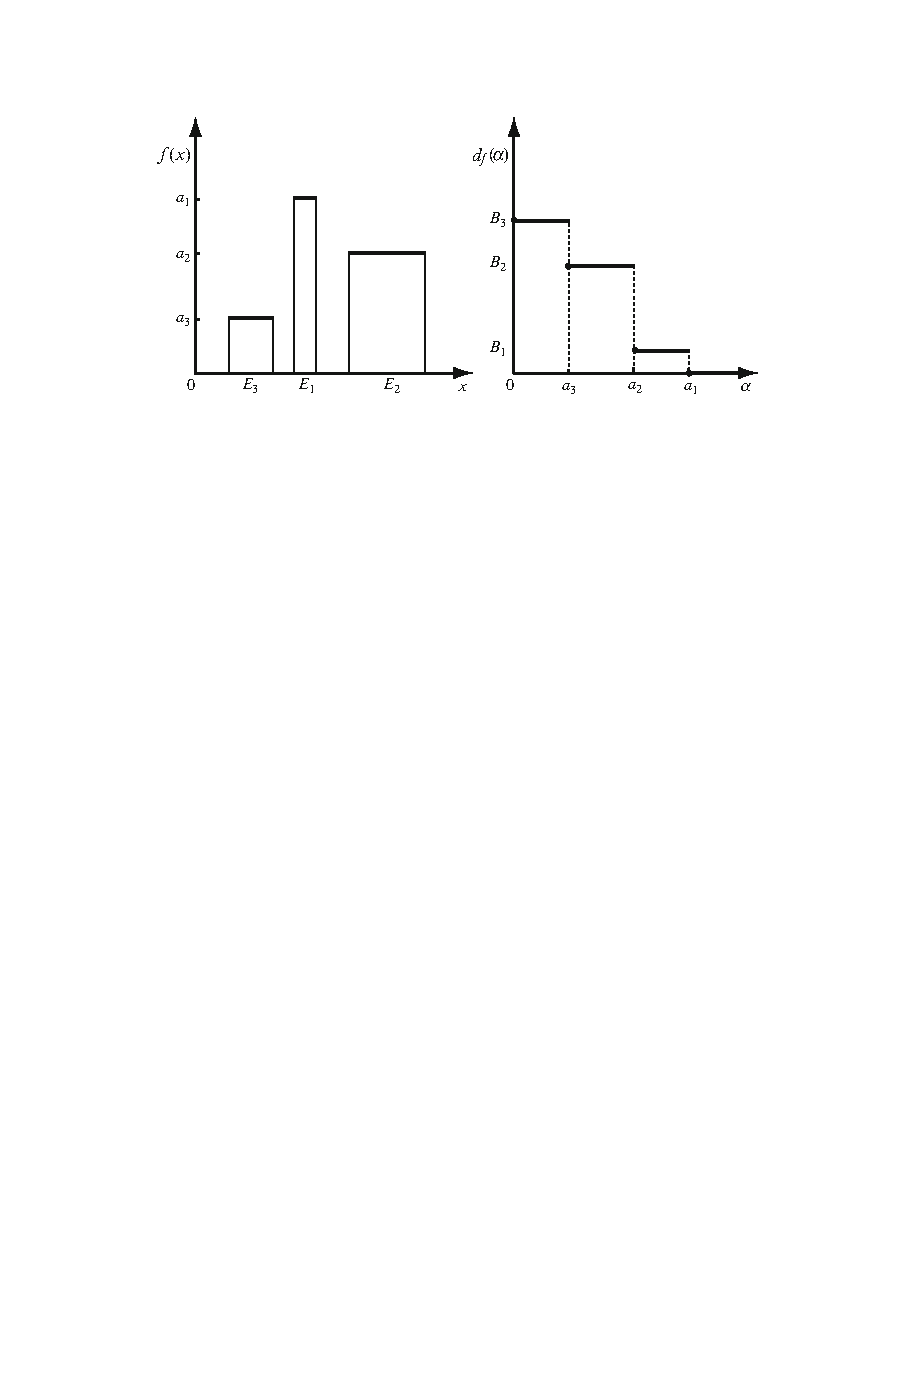
\includegraphics{pictures/distribution-of-simple}
\caption{The graph of a simple function and its distribution function.}
\end{figure}
We compile the basic properties of $\lambda_f$ in a proposition:
\begin{proposition}\label{distribution function prop}
Let $(X,\mathcal{A},\mu)$ be a measure space. Let $f$ and $g$ be $\mathcal{A}$-measurable functions on $X$. Then
\begin{itemize}
\item[(a)] $\lambda_f$ is decreasing and right continuous.
\item[(b)] If $|f|\leq|g|$ a.e.then $\lambda_f\leq\lambda_g$.
\item[(c)] if $|f_n|$ increases to $|f|$, then $\lambda_{f_n}$ increases to $f$.
\item[(d)] $\lambda_{cf}(\alpha)=\lambda_f(\alpha/|c|)$.
\item[(e)] $\lambda_{f+g}(\alpha+\beta)\leq\lambda_f(\alpha)+\lambda_g(\beta)$ and $\lambda_{fg}(\alpha\beta)\leq\lambda_f(\alpha)\lambda_g(\beta)$.   
\end{itemize}
\end{proposition}
\begin{proof}
Let $E_\alpha(f)=\{x:|f(x)|>\alpha\}$. The function $\lambda_f$ is decreasing since $E_\alpha(f)\sups E_\beta(f)$ if $\alpha<\beta$, and it is right continuous since $E_\alpha(f)$ is the increasing union of $\{E_{\alpha+1/n}(f)\}$.\par
If $|f|\leq|g|$, then $E_\alpha(f)\sub E_\alpha(g)$, so $\lambda_f\leq\lambda_g$. If $|f_n|$ increases to $|f|$, then $E_\alpha(f)$ is the increasing union of $\{E_\alpha(f_n)\}$, so $\lambda_{f_n}$ increases to $\lambda_f$.\par
Now for $c\in\C^*$, we have $E_\alpha(cf)=E_{\alpha/|c|}(f)$, so $\lambda_{cf}(\alpha)=\lambda_f(\alpha/|c|)$. Finally, since $|f+g|\leq|f|+|g|$, we have $E_{\alpha+\beta}(f)\sub E_\alpha(g)\cup E_\beta(h)$, which implies that $\lambda_f(\alpha+\beta)\leq\lambda_g(\alpha)+\lambda_h(\beta)$. The second inequality can be proved similarly
\end{proof}
Suppose that $\lambda_\alpha<+\infty$ for all $\alpha>0$. In view of Proposition~\ref{distribution function prop}, $\lambda_f$ defines a negative Borel measure $\nu$ on $(0,+\infty)$ such that $\nu((a,b])=\lambda_f(b)-\lambda_f(a)$ whenever $0<a<b$. We can therefore consider the Lebesgue-Stieltjes integrals $\int\phi\,d\lambda_f=\int\phi\,d\nu$ of functions $\phi$ on $(0,+\infty)$. The following result shows that the integrals of functions of $|f|$ on $X$ can be reduced to such Lebesgue-Stieltjes integrals.
\begin{proposition}\label{distribution integral prop}
Let $(X,\mathcal{A},\mu)$ be a measure space and $f$ be a measurable function on $X$. If $\lambda_f(\alpha)<+\infty$ for all $\alpha>0$ and $\phi$ is a nonnegative Borel measurable function on $(0,+\infty)$, then
\[\int_X\phi(|f|)\,d\mu=-\int_{0}^{+\infty}\phi(\alpha)\,d\lambda_f(\alpha).\]
\end{proposition}
\begin{proof}
Note that
\[-\nu((a,b])=-(\lambda_f(b)-\lambda_f(a))=\lambda_f(a)-\lambda_f(b)=\mu(\{x:a<|f(x)|\leq b\})=\mu(|f|^{-1}((a,b])).\]
It follows that $-\nu=|f|_*\mu$ by the uniqueness of extensions. Thhus Proposition~\ref{measure push out by measurable function prop} implies the claim.
\end{proof}
The case of this result in which we are most interested is $\phi(\alpha)=\alpha^p$, which gives
\[\int|f|^p\,d\mu=-\int_{0}^{+\infty}\alpha^p\,d\lambda_f(\alpha).\]
A more useful form of this equation is obtained by integrating the right side by parts.
\begin{corollary}
Let $(X,\mathcal{A},\mu)$ be a measure space. If $0<p<+\infty$, then
\begin{align}\label{L^p norm integral by distribution}
\int|f|^p\,d\mu=p\int_0^{+\infty}\alpha^{p-1}\lambda_f(\alpha)\,d\alpha.\end{align}
\end{corollary}
\begin{proof}
If $\lambda_f(\alpha)=+\infty$ for some $\alpha>0$, then both integrals are infinite. If not, and $f$ is simple, then $\lambda_f$ is bounded as $\alpha\to 0$ and vanishes for a sufficiently large, so integration by parts works. For the general case, let $\{\phi_n\}$ be a sequence of simple functions such that $|\phi_n|$ increases to $|f|$; then the desired result is true for $g_n$. For each $\eps>0$, we can choose $\phi_n$ such that $\|f-\phi_n\|_p<\eps$. Then by Chebyshev's inequality we have
\begin{align*}
\varlimsup_{\alpha\to 0}\alpha^p\lambda_f(\alpha)&\leq\varlimsup_{\alpha\to 0}\alpha^p\lambda_{f-\phi_n}(\alpha/2)+\varlimsup_{\alpha\to 0}\alpha^p\lambda_{f-\phi_n}(\alpha/2)\\
&\leq\varlimsup_{\alpha\to 0}2^p\|f-\phi_n\|_p^p+\varlimsup_{\alpha\to 0}2^p\alpha^p\lambda_{f-\phi_n}(\alpha)\leq\eps.
\end{align*}
Thus we see $\lim_{\alpha\to 0}\alpha^p\lambda_f(\alpha)=0$. Similarly, we can prove that $\lim_{\alpha\to+\infty}\alpha^p\lambda_{f}(\alpha)=0$, thus the claim follows by integration by parts.
\end{proof}
We thus have a totally alternative method for computing $L^p$ norms which is extremely useful, as we will see shortly. Observe in particular, a function has finite $L^p$ norm, for $p<+\infty$, if its distribution function decays just slightly faster than $1/\alpha^p$ as $\alpha\to+\infty$, while it explodes to $+\infty$ as $\alpha\to 0$ just slightly slower than $1/\alpha^p$. If a function $f$ has a distribution function of the order exactly $1/\alpha^p$ as $\alpha\to+\infty$ or $\alpha\to 0$, then the integral just barely fails to be finite, as it will diverge logarithmically at these extremes. We say such functions are in weak $L^p$.\par
If $f$ is a measurable function on $X$ and $0<p<+\infty$, we define
\[\|f\|_{p,\infty}=\sup\{\alpha\lambda_f(\alpha)^{1/p}:\alpha>0\}=\inf\{C\geq 0:\alpha^p\lambda_f(\alpha)\leq C^p\text{ for all $\alpha>0$}\}\]
and we define \textbf{weak $\bm{L^p}$} to be the set $L^{p,\infty}(X,\mathcal{A},\mu)$ of all $f$ such that $\|f\|_{p,\infty}<+\infty$. The space $L^{\infty,\infty}(X,\mathcal{A},\mu)$ is by definition $L^p(X,\mathcal{A},\mu)$. The properties of $\|\cdot\|_{p,+\infty}$ are listed bolow.
\begin{lemma}\label{weak L^p norm prop}
Let $(X,\mathcal{A},\mu)$ be a measure space and $0<p\leq+\infty$.
\begin{itemize}
\item[(a)] For $c\in\C^*$ we have $\|cf\|_{p,\infty}=|c|\cdot\|f\|_{p,\infty}$.
\item[(b)] If $\|f\|_{p,\infty}=0$ then $f=0$ a.e.
\item[(c)] For $f,g\in L^p(X,\mathcal{A},\mu)$ we have
\[\|f+g\|_{p,\infty}\leq 2^{\max\{1,1/p\}}(\|f\|_{p,\infty}+\|g\|_{p,\infty}).\]
\end{itemize}
Therefore, the space $L^{p,\infty}(X,\mathcal{A},\mu)$ is a quasi-normed vector space.
\end{lemma}
\begin{proof}
From Proposition~\ref{distribution function prop} we get (a). For (b), if $\|f\|_{p,\infty}=0$, then $\lambda_f(\alpha)=0$ for all $\alpha>0$, which means $\{x:f(x)\neq 0\}$ is null, so $f=0$ a.e. Finally, since $(a+b)^p\leq 2^{\max\{1,p\}-1}(a^p+b^p)$ for all $a,b,p>0$, we have
\begin{equation*}\small
\begin{aligned}
\alpha\lambda_f(\alpha)^{1/p}\leq 2^{\max\{1,1/p\}}[(\alpha/2)\lambda_f(\alpha/2)^{1/p}+(\alpha/2)\lambda_f(\alpha/2)^{1/p}]\leq 2^{\max\{1,1/p\}}(\|f\|_{p,+\infty}+\|g\|_{p,+\infty}).
\end{aligned}
\end{equation*}
This proves the claim.
\end{proof}
The relationship between $L^p$ and weak $L^p$ is as follows.
\begin{proposition}\label{L^p is weak L^p}
For any $0<p<+\infty$ and any $f$ in $L^p(X,\mathcal{A},\mu)$ we have
\[\|f\|_{p,\infty}\leq\|f\|_p.\]
Thus we have a continuous embedding $L^p(X,\mathcal{A},\mu)\sub L^{p,\infty}(X,\mathcal{A},\mu)$.
\end{proposition}
\begin{proof}
This is just a trivial consequence of Chebyshev's inequality:
\[\alpha^p\lambda_f(\alpha)\leq\|f\|_p^p.\]
Using the definition of $\|\cdot\|_{p,\infty}$, we obtain the claim.
\end{proof}
If we replace $\lambda_f(\alpha)$ by $(\|f\|_{p,\infty}/\alpha)^p$ in the integral $\int_{0}^{+\infty}\alpha^{p-1}\lambda_f(\alpha)\,d\alpha$, which equals $\|f\|_p^p$, we obtain a constant times $\int_{0}^{+\infty}\alpha^{-1}d\alpha$, which is divergent at both $0$ and $+\infty$. One needs only slightly stronger estimates on $\lambda_f$ near $0$ and $+\infty$ to obtain
$f\in L^p$. The standard example of a function that is in weak $L^p$ but not in $L^p$ is $f(x)=|x|^{-n/p}$ on $\R^n$. Its distribution functions satisfy
\[\lambda_f(\alpha)=\lambda(\{x:|x|^{-n/p}>\alpha\})=\lambda(\{x:|x|\leq\alpha^{-p/n}\})=\lambda(B_{\alpha^{-p/n}}(0))=\frac{\omega_n}{\alpha^{p}},\]
where $\omega_n$ is the measure of the unit ball of $\R^n$. So we have $\|f\|_{p,\infty}=\omega_n^{1/p}$.\par
However, under certain bounded condition, we can go from weak $L^p$ to $L^p$.
\begin{proposition}\label{weak L^p is L^p if}
Let $(X,\mathcal{A},\mu)$ be a measure space and $0<p\leq+\infty$. Let $f\in L^{p,\infty}(X,\mathcal{A},\mu)$.
\begin{itemize}
\item[(a)] If $\mu(\{x:f(x)\neq 0\})<+\infty$, then $f\in L^{q}(X,\mathcal{A},\mu)$ for all $q<p$.
\item[(b)] If $f$ is bounded, then $f\in L^q(X,\mathcal{A},\mu)$ for all $q>p$.
\end{itemize} 
\end{proposition}
\begin{proof}
If $f\in L^{p,\infty}(X,\mathcal{A},\mu)$ and $\mu(\{x:f(x)\neq 0\})<+\infty$ then $\lambda_f(\alpha)$ is bounded. Let $C=\|f\|_{p,\infty}^p$, for $q<p$ we have
\[\int_{1}^{+\infty}\alpha^{q-1}\lambda_f(\alpha)\,d\alpha\leq C\int_{1}^{+\infty}\alpha^{q-p-1}d\alpha<+\infty.\]
Thus we see $f\in L^q(X,\mathcal{A},\mu)$ for all $q<p$.\par
Similarly, if $f$ is bounded, then $\lambda_f(\alpha)$ is zero for sufficiently large $\alpha$. Also, for $q>p$ we have
\[\int_{0}^{1}\alpha^{q-1}\lambda_f(\alpha)\,d\alpha\leq C\int_{0}^{1}\alpha^{q-p-1}\,d\alpha<+\infty.\]
Thus $f\in L^q(X,\mathcal{A},\mu)$ in this case.
\end{proof}
Similarly to the $L^p$-spaces, we will interchangeably regard $L^{p,+\infty}$ as a set of functions as well as a vector space on equivalence classes of functions modulo modifications on $\mu$-null sets. The space $L^{p,+\infty}$ is naturally endowe with topology induced by the quasi-norm $\|\cdot\|_{p,+\infty}$. By Lemma~\ref{weak L^p norm prop}, the operations of addition and scalar multiplications are continuous which makes $L^{p,+\infty}$ a topological vector space. The topology is first countable and so convergence can be defined using sequences. We thus say that $f_n\to f$ in $L^{p,+\infty}$ if $\|f_n-f\|_{p,+\infty}\to 0$. (Note that this is not related to the weak convergence despite the unfortunate use of the word "weak".) A sequence $\{f_n\}$ is Cauchy if $\|f_n-f_m\|\to 0$ as $m,n\to 0$. We now claim that $L^{p,+\infty}$ is complete for $0<p\leq+\infty$. This claim is immediate, once we note the following fact:
\begin{proposition}
Let $(X,\mathcal{A},\mu)$ be a measure space and $0<p\leq+\infty$. Let $\{f_n\}$ and $f$ be measurable functions such that $\{f_n\}$ converges to $f$ in weak $L^p$. Then $\{f_n\}$ converges to $f$ in measure.
\end{proposition}
\begin{proof}
For $\eps>0$, we have
\[\mu(\{x:|f(x)-f_n(x)|>\eps\})=\lambda_{|f-f_n|}(\eps)\leq\frac{\|f-f_n\|_{p,+\infty}^p}{\eps^p}\to 0.\]
Thus the claim follows.
\end{proof}
\begin{proposition}\label{weak L^p complete}
For any $p\in(0,+\infty]$, the space $L^{p,+\infty}$ is complete.
\end{proposition}
\begin{proof}
Since $L^{+\infty,+\infty}=L^+\infty$, we focus on $p\in(0,+\infty)$. Let $\{f_n\}$ be a Cauchy sequence in $L^{p,+\infty}$. Then we now that $\{f_n\}$ is Cauchy in measure, so by Theorem~\ref{convergence in measure subsequence converge a.e.} there exists a subsequence $\{f_{n_k}\}$ and a function $f$ such that $f_{n_k}\to f$ almost everywhere. Fatou’s lemma then implies
\[\alpha\mu(\{|f_n-f|>\alpha\})^{1/p}\leq\alpha\varlimsup_m\mu(\{|f_n-f_m|>\alpha\})^{1/p}\leq\varlimsup_m\|f-f_n\|_{p,+\infty}.\]
Hence $\|f_n-f\|_{p,\infty}\to 0$ and, by Lemma~\ref{weak L^p norm prop}, also $f$ in $L^{p,+\infty}$.
\end{proof}
\begin{example}
Note that there is no general converse of the statement in the preceding proposition. Fix $0<p<+\infty$ and on $[0,1]$ define the functions
\[f_n(x)=k^{1/p}\chi_{[j/k,(j+1)/k]}\ \text{where $n=k+j$ and $j\leq k$}.\]
Then clearly $f_n$ converges to $0$ in measure. Likewise, observe that
\[\|f_n\|_{p,\infty}=\sup\{\alpha\lambda_{f_n}(\alpha)^{1/p}:\alpha>0\}\geq k^{1/p}\lambda_{f_n}(k^{1/p})=1.\]
which implies that $f_n$ does not converge to $0$ in $L^{p,\infty}$.
\end{example}
The theory of the weak $L^p$ spaces seems to run parallel to that of $L^p$-spaces except for one important defect: $\|\cdot\|_{p,+\infty}$ is not a norm (just a quasi-norm) due to the lack of the triangle inequality. This can be mended as follows:
\begin{proposition}\label{weak L^p normability and metrizability}
Let $(X,\mathcal{A},\mu)$ be a measure space and $0<r<p<+\infty$. For any $f\in L^{p,+\infty}$, we have
\begin{align}\label{weak L^p normability and metrizability-1}
\|f\|_{p,+\infty}\leq\inf\Big\{C\geq 0:\Big(\int_A|f|^r\Big)^{1/r}\leq C\mu(A)^{1/r-1/p}\text{ for all $\mu(A)<+\infty$}\Big\}\leq\frac{p}{p-r}\|f\|_{p,+\infty}.
\end{align}
Therefore, for any $0<r<p$, the function defined by
\begin{align}\label{weak L^p normability and metrizability-2}
\rho_{p,r}(f):=\sup_{0<\mu(A)<+\infty}\frac{(\int_A|f|^r)^{1/r}}{\mu(A)^{1/r-1/p}}=\inf\Big\{C\geq 0:\Big(\int_A|f|^r\Big)^{1/r}\leq C\mu(A)^{1/r-1/p},\mu(A)<+\infty\Big\}
\end{align}
is equivalent to the quasi-norm $\|\cdot\|_{p,+\infty}$. In particular, $L^{p,+\infty}(X,\mathcal{A},\mu)$ is normable for $p>1$.
\end{proposition}
\begin{proof}
We first establish $(\ref{weak L^p normability and metrizability-1})$. Pick $C\geq 0$ in the set above, then for any $\alpha>0$, we have
\[\alpha\mu(\{|f|>\alpha\})\leq\int_{\{|f|>\alpha\}}|f|\leq C\mu(A)^{1-1/p},\]
which simplifies to $\alpha\mu(\{|f|>\alpha\})^{1/p}\leq C$. Thus $\|f\|_{p,+\infty}$ is smaller that the infimum in $(\ref{weak L^p normability and metrizability-1})$. Conversely, for $A\in\mathcal{A}$ with $\mu(A)<+\infty$ and $C>0$ such that $\alpha\lambda_f(\alpha)^{1/p}\leq C$, by $(\ref{L^p norm integral by distribution})$ we have
\begin{equation*}\small
\begin{aligned}
\int_A|f|&=\int_{0}^{+\infty}\mu(\{x:|f(x)\chi_A(x)|>\alpha\})\,d\alpha=\int_{0}^{+\infty}\mu(\{x:|f(x)|>\alpha\}\cap A)\,d\alpha\\
&\leq\int_{0}^{+\infty}\min\{C^p\alpha^{-p},\mu(A)\}\,d\alpha=\int_{0}^{\frac{C}{\mu(A)^{1/p}}}\mu(A)\,d\alpha+\int_{\frac{C}{\mu(A)^{1/p}}}^{+\infty}\frac{C^p}{\alpha^p}\,d\alpha\\
&=C\mu(A)^{1-1/p}+\frac{C^p}{p-1}\frac{C^{1-p}}{\mu(A)^{(1-p)/p}}=C\mu(A)^{1-1/p}+\frac{C}{p-1}\mu(A)^{1-1/p}=\frac{pC}{p-1}\mu(A)^{1-1/p}.
\end{aligned}
\end{equation*}
Since this holds for any such $C>0$, we conclude the second part in $(\ref{weak L^p normability and metrizability-1})$.\par
Now by $(\ref{weak L^p normability and metrizability-1})$ it is clear that the function defined by $(\ref{weak L^p normability and metrizability-1})$ is equivalent to $\|\cdot\|_{p,+\infty}$. Since the $L^p$ quasi-norm is a norm for $p>1$, this implies $L^{p,+\infty}(X,\mathcal{A},\mu)$ is normable for $p>1$.
\end{proof}
\begin{example}
Suppose that $(X,\mathcal{A},\mu)$ is such that $\mu$ is non-zero and non-atomic. Then we claim that the topology on $L^{1,+\infty}$ cannot be normed. In fact, since $\mu$ is non-atomic, we can construct a decreasing sequence $\{A_n\}$ with $\mu(A_n)\to 0$. Now define
\[f_n=\sum_{i=1}^{n}h_i,\ \ \text{where}\ \ h_i=\frac{\chi_{A_i\setminus A_{i+1}}}{\mu(A_i)}.\]
Now fix $\alpha>0$. Since $\mu(A_n)\to 0$, there exists $N>0$ such that $\mu(A_{N-1})^{-1}<\alpha\leq\mu(A_{N})^{-1}$. Then
\[\alpha\mu(\{|f_n|>\alpha\})\leq\frac{1}{\mu(A_{N})}\mu(A_{N}\cap\supp(f_n))\leq 1.\]
Thus $\|f_n\|_{1,+\infty}\leq 1$ for all $n$. On the other hand,
\[\|h_n\|_{1,+\infty}=\frac{\mu(A_n\setminus A_{n+1})}{\mu(A_n)}=1-\frac{\mu(A_{n+1})}{\mu(A_n)}.\]
Since $\mu(A_n)\to 0$, we know the series $\sum_{n}\|h_n\|_{1,+\infty}$ diverges. This shows that the ratio $\sum_{n}\|h_n\|_{1,+\infty}$ and $\|\sum_nh_n\|_{1,+\infty}$ can be made arbitrary large, which rules out that $\|\cdot\|_{1,+\infty}$ is equivalent to a norm.
\end{example}
\section{The Marcinkiewicz interpolation theorem, diagonal form}
Weak-type inequalities, or estimates, are bounds that enable control of the weak $L^p$ quasi-norms. Of particular importance, are those operators from a vector space of measurable functions on a space $(X,\mathcal{A},\mu)$ to measurable functions on another space $(Y,\mathcal{B},\nu)$ for which weak and strong $L^q$ norms on $Y$ can be controlled by strong $L^p$ norms on $X$. We are interested in a slightly more general class of operators than just the linear ones, so we introduce \textbf{sublinear operators} as those that satisfy
\[|T(f+g)|\leq|Tf|+|Tg|,\quad |T(cf)|=c|Tf|\]
for all $f,g$ in its domain and $c>0$.
\begin{definition}
Let $0<p,q\leq +\infty$ and $T$ a sublinear operator from a vector space of measurable functions on $(X,\mathcal{A},\mu)$ that includes $L^p(X,\mathcal{A},\mu)$ to measurable functions on $(Y,\mathcal{B},\nu)$. We say that
\begin{itemize}
\item $T$ is \textbf{weak type $(p,q)$} if $Tf\in L^{q,\infty}(Y,\mathcal{B},\nu)$ for all $f\in L^p(X,\mathcal{A},\mu)$ and there exists $C\geq 0$ such that
\[\|Tf\|_{q,\infty}\leq C\|f\|_{p}.\]
\item $T$ is \textbf{strong type $(p,q)$} if $Tf\in L^{q}(Y,\mathcal{B},\nu)$ for all $f\in L^p(X,\mathcal{A},\mu)$ and there exists $C\geq 0$ such that
\[\|Tf\|_{q}\leq C\|f\|_{p}.\]
\end{itemize}
Clearly, from Proposition~\ref{L^p is weak L^p} we conclude that strong type $(p,q)$ operators are also weak type $(p,q)$. And, strong type $(p,+\infty)$ is the same as weak type $(p,+\infty)$.
\end{definition}
We begin by noting a simple interpolation fact for the quasinorms:
\begin{proposition}[\textbf{Interpolation for Weak $\bm{L^p}$ Norms}]\label{interpolation for weak norms}
Let $(X,\mathcal{A},\mu)$ be a measure space, and $0<p_0,p_1\leq+\infty$. For $t\in[0,1]$ define
\[\frac{1}{p}=\frac{1-t}{p_0}+\frac{t}{p_1}.\]
Then for any $f\in L^0(X,\mathcal{A},\mu)$ we have
\begin{align}\label{interpolation for weak norms-1}
\|f\|_{p,+\infty}\leq\|f\|_{p_0,+\infty}^{1-t}\|f\|_{p_1,+\infty}^t.
\end{align}
Moreover, if $p_0<p_1$, then for $t\in(0,1)$,
\begin{align}\label{interpolation for weak norms-2}
\|f\|_{p}\leq\Big(\frac{p}{p-p_0}+\frac{p}{p_1-p}\Big)^{1/p}\|f\|_{p_0,+\infty}^{1-t}\|f\|_{p_1,+\infty}^t.
\end{align}
\end{proposition}
\begin{proof}
Assuming $f\neq 0$ and $p_0,p_1<+\infty$, for each $\alpha>0$ we have
\[\alpha\lambda_f(\alpha)^{1/p}=\alpha^{1-t}\lambda_f(\alpha)^{(1-t)/p_0}\cdot\alpha^{t}\lambda_f(\alpha)^{t/p_1}\leq\|f\|_{p_0}^{1-t}\|f\|_{p_1}^t.\]
Taking supremum over $\alpha>0$ gives $(\ref{interpolation for weak norms-1})$. The case when $p_0<p_1=+\infty$ follows by noting that then $1/p=(1-t)/p_0$ and the supremum can be reduced to $\alpha\leq\|f\|_{\infty}$.\par
For the second part of the claim, we assume first $p_1<+\infty$ and recall the identity $(\ref{L^p norm integral by distribution})$ to write, for any $A>0$,
\begin{align}\label{interpolation for weak norms-3}
\|f\|_{p}^{p}=\int_{0}^{A}p\alpha^{p-1}\lambda_f(\alpha)\,d\alpha+\int_{A}^{+\infty}p\alpha^{p-1}\lambda_f(\alpha)\,d\alpha.
\end{align}
Using the definitions of $\|f\|_{p_0,+\infty}$ and $\|f\|_{p_1,+\infty}$ along with $p_0<p<p_1$, this becomes
\begin{equation}\label{interpolation for weak norms-4}
\begin{aligned}
\|f\|_{p}^{p}&\leq p\|f\|_{p_0,+\infty}^{p_0}\int_{0}^{A}\alpha^{p-p_0-1}\,d\alpha+p\|f\|_{p_1,+\infty}^{p_1}\int_{A}^{+\infty}\alpha^{p-p_1-1}\lambda_f(\alpha)\,d\alpha\\
&=\frac{p}{p-p_0}\|f\|_{p_0,+\infty}^{p_0}A^{p-p_0}+\frac{p}{p_1-p}\|f\|_{p_1,+\infty}^{p_1}A^{p-p_1}.
\end{aligned}
\end{equation}
Since this inequality holds for all $a$, we want to choose $A$ to minmize the right-side of $(\ref{interpolation for weak norms-4})$. We observe that
\[\|f\|_{p_0,+\infty}^{p_0}A^{p-p_0}=\|f\|_{p_1,+\infty}^{p_1}A^{p-p_1}\Longrightarrow A=\Big(\frac{\|f\|_{p_1,+\infty}^{p_1}}{\|f\|_{p_0,+\infty}^{p_0}}\Big)^{\frac{1}{p_1-p_0}}.\] 
Choosing such $A$, we then get
\begin{align*}
\|f\|_{p_0,+\infty}^{p_0}A^{p-p_0}&=\|f\|_{p_0,+\infty}^{p_0}\Big(\frac{\|f\|_{p_1,+\infty}^{p_1}}{\|f\|_{p_0,+\infty}^{p_0}}\Big)^{\frac{p-p_0}{p_1-p_0}}=(\|f\|_{p_0,+\infty}^{p_0})^{\frac{p_1-p}{p_1-p_0}}(\|f\|_{p_1,+\infty}^{p_1})^{\frac{p-p_0}{p_1-p_0}}\\
&=(\|f\|_{p_0,+\infty})^{p\cdot\frac{\frac{1}{p}-\frac{1}{p_1}}{\frac{1}{p_0}-\frac{1}{p_1}}}(\|f\|_{p_1,+\infty})^{p\cdot\frac{\frac{1}{p_0}-\frac{1}{p}}{\frac{1}{p_0}-\frac{1}{p_1}}}=(\|f\|_{p_0,+\infty})^{(1-t)p}(\|f\|_{p_1,+\infty})^{tp}
\end{align*}
Insert this into $(\ref{interpolation for weak norms-4})$ and take $p$-th root, we then get $(\ref{interpolation for weak norms-2})$. In the case when $p_1=+\infty$ we take $A=\|f\|_{\infty}$, which eliminates the second integral above.
\end{proof}
Now we present the Marcinkiewicz Interpolation Theorem. Here we only prove a diagonal form. The general form will be proved when we introduce Lorentz spaces.
\begin{theorem}[\textbf{Marcinkiewicz Interpolation Theorem, Diagonal form}]\label{Marcinkiewicz interpolation diagonal}
Let $(X,\mathcal{A},\mu)$ be a $\sigma$-finite measure space and $(Y,\mathcal{B},\nu)$ be another measure space. Let $0<p_0<p_1\leq+\infty$ and let $T:(L^{p_0}+L^{p_1})(X,\mathcal{A},\mu)\to L^0(Y,\mathcal{B},\nu)$ be sublinear a sublinear operator and for $t\in[0,1]$ define
\[p:=\frac{1-t}{p_0}+\frac{t}{p_1}.\]
If there exist constants $C_0$, $C_1$ such that
\[\|Tf\|_{p_0,\infty}\leq C_0\|f\|_{p_0},\quad \|Tf\|_{p_1,\infty}\leq C_1\|f\|_{p_1}.\]
Then for all $t\in(0,1)$ we have
\[\|Tf\|_{p}\leq 2\Big(\frac{p}{p-p_0}+\frac{p}{p_1-p}\Big)^{1/p}C_0^{1-t}C_1^t\|f\|_p.\]
\end{theorem}
\begin{proof}
Assume first that $p_1<+\infty$. Fix $f$ a function in $L^{p}(\mu)$ and $\alpha>0$. We split $f=f_0+f_1$, where $f_0$ is in $L^{p_0}$ and $f_1$ is in $L^{p_1}$. The splitting is obtained by cutting $|f|$ at height $A\alpha$ for some $A>0$ to be determined later. Set
\[f_0=f\chi_{\{|f|>A\alpha\}},\quad f_1=f\chi_{\{|f|\leq A\alpha\}}.\]
These functions depend on $\alpha$ without that being explicit in the notation. It can be checked easily that $f_0$ (the unbounded part of $f$) is an $L^{p_0}$ function and that $f_1$ (the bounded part of $f$) is an $L^{p_1}$ function. Indeed, since $p_0<p$, we have
\[\|f_0\|_{p_0}^{p_0}=\int_{\{|f|>A\alpha\}}|f|^{p_0}=\int_{\{|f|>A\alpha\}}|f|^{p_0-p}|f|^{p}\leq(A\alpha)^{p_0-p}\|f\|_{p}^{p},\]
and
\[\|f_1\|_{p_1}^{p_1}=\int_{\{|f|\leq A\alpha\}}|f|^{p_1}=\int_{\{|f|>A\alpha\}}|f|^{p_1-p}|f|^{p_1}\leq(A\alpha)^{p_1-p}\|f\|_{p}^{p}.\]
As $f=f_0+f_1$, the sublinearity of $T$ and a union bound give $\lambda_{Tf}(2\alpha)\leq\lambda_{Tf_0}(\alpha)+\lambda_{Tf_1}(\alpha)$. We now calculate, using $(\ref{L^p norm integral by distribution})$ and the assumption on $T$, that
\begin{equation*}\small
\begin{aligned}
\|Tf\|_{p}^{p}&=p\int_{0}^{+\infty}\alpha^{p-1}\lambda_{Tf}(\alpha)\,d\alpha\leq p\int_{0}^{+\infty}\alpha^{p-1}[\lambda_{Tf_0}(\alpha/2)+\lambda_{Tf_1}(\alpha/2)]d\alpha\\
&\leq p\int_{0}^{+\infty}\alpha^{p-1}\Big[\Big(\frac{\|Tf_0\|_{p_0,\infty}}{\alpha/2}\Big)^{p_0}+\Big(\frac{\|Tf_1\|_{p_1,\infty}}{\alpha/2}\Big)^{p_1}\Big]d\alpha\\
&\leq p\int_{0}^{+\infty}\alpha^{p-1}\Big[\Big(\frac{C_0\|f_0\|_{p_0}}{\alpha/2}\Big)^{p_0}+\Big(\frac{C_1\|f_1\|_{p_1}}{\alpha/2}\Big)^{p_1}\Big]d\alpha\\
&=p\int_{0}^{+\infty}\Big[(2C_0)^{p_0}\alpha^{p-p_0-1}\int_{\{|f|>A\alpha\}}|f|^{p_0}+(2C_1)^{p_1}\alpha^{p-p_1-1}\int_{\{|f|\leq A\alpha\}}|f|^{p_1}\Big]d\alpha.
\end{aligned}
\end{equation*}
Using Tonelli's theorem, the two integrals can be calculated as follows
\begin{align*}
\int_{0}^{+\infty}\alpha^{p-p_0-1}\int_{\{|f|\leq A\alpha\}}|f(x)|^{p_0}\,dx d\alpha=\int_{X}|f(x)|^{p_0}dx\int_{0}^{\frac{|f(x)|}{A}}\alpha^{p-p_0-1}d\alpha=\frac{\int_X|f|^{p}}{(p-p_0)A^{p-p_0}},
\end{align*}
and
\begin{align*}
\int_{0}^{+\infty}\alpha^{p-p_1-1}\int_{\{|f|>A\alpha\}}|f(x)|^{p_1}dx d\alpha=\int_{X}|f(x)|^{p_1}dx\int_{\frac{|f(x)|}{A}}^{+\infty}\alpha^{p-p_1-1}\,d\alpha=\frac{\int_X|f|^{p}}{(p_1-p)A^{p-p_1}}.
\end{align*}
Thus we conclude that
\begin{align}\label{Marcinkiewicz interpolation diagonal-1}
\|Tf\|_{p}^{p}\leq p\Big[\frac{(2C_0)^{p_0}}{(p-p_0)A^{p-p_0}}+\frac{(2C_1)^{p_1}}{(p_1-p)A^{p-p_1}}\Big]\int|f|^{p}.
\end{align}
In order to get the inequality, we observe that
\[\frac{(2C_0)^{p_0}}{A^{p-p_0}}=\frac{(2C_1)^{p_1}}{A^{p-p_1}}\Longrightarrow A=2^{-1}\Big(\frac{C_0^{p_0}}{C_1^{p_1}}\Big)^{\frac{1}{p_1-p_0}}\Longrightarrow \frac{(2C_0)^{p_0}}{A^{p-p_0}}=2^{p}C_0^{(1-t)p}C_1^{tp}.\]
Thus the claim follows in this case. For $p_1=+\infty$ we use that $\|Tf\|_{+\infty,+\infty}=\|Tf\|_\infty$ and so by the assumption
\[\|Tf_1\|_\infty\leq C_1\|f_1\|_\infty=C_1A\alpha.\]
For $A=(2C_1)^{-1}$ this gives $\lambda_{Tf_1}(\alpha/2)=0$. This eliminates the second term in the large bracket on the right of $(\ref{Marcinkiewicz interpolation diagonal-1})$, which can just as well be achieved (for the above choice of $A$) by taking $p_1\to+\infty$ there.
\end{proof}
As an application, we consider the Hardy-Littlewood maximal operator $H$ defined by
\[Hf(x)=\sup_{r>0}\frac{1}{\lambda(B_r(x))}\int_{B_r(x)}|f(y)|\,dy\quad f\in L^1_{\loc}(\R^n).\]
$H$ is obviously sublinear and satisfies $\|Hf\|_{\infty}\leq\|f\|_\infty$ for all $f\in L^\infty$. Moreover, Theorem~\ref{maximal operator weak 1,1} says precisely that $H$ is weak type $(1,1$). We conclude:
\begin{corollary}
There is a constant $C>0$ such that if $1<p<+\infty$ and $f\in L^p(\R^n)$ then
\[\|Hf\|_p\leq C\|f\|_p.\]
\end{corollary}
\section{Lorentz spaces}
To explore generalizations of our interpolation theorems, we now consider a new type of spaces which effectively generalize $L^p$ and weak $L^p$ spaces.
\subsection{Decreasing rearrangements}
Suppose that $f$ is a measurable function on a measure space $(X,\mathcal{A},\mu)$. To manipulate the distribution function $\lambda_f$ effectively, it would be desirable to have another function $f^*$ defined on $[0,+\infty)$ that is decreasing and equidistributed with $f$, by which we mean
\[\lambda_f(\alpha)=\lambda_{f^*}(\alpha),\ \forall\alpha>0.\]
This is achieved via a simple construction discussed below.
\begin{definition}
Let $f$ be a $\mathcal{A}$-measurable function defined on $X$. The \textbf{decreasing rearrangement} of $f$ is the function $f^*$ defined on $[0,+\infty)$ by
\[f^*(t)=\inf\{\alpha>0:\lambda_f(\alpha)\leq t\},\]
where we adopt the convention $\inf\emp=+\infty$, thus having $f^*(t)=+\infty$ whenever $\lambda_f(\alpha)>t$ for all $\alpha\geq 0$. Observe that $f^*$ is decreasing and supported in $[0,\mu(X)]$.
\end{definition}
Before preceeding, we frist see some examples.
\begin{example}\label{decreasing rearrangement of simple}
Consider the simple function of Example~\ref{distribution of simple function},
\[f(x)=\sum_{i=1}^{n}a_i\chi_{E_i}(x),\]
where $E_i$ are pairwise disjoint sets of finite measure and $a_1>\cdots>a_n>0$. We saw in Example~\ref{distribution of simple function} that
\[\lambda_f(\alpha)=\sum_{j=0}^{n}B_j\chi_{[a_{j+1},a_j)}(\alpha)\ \ \text{where}\ \ B_j=\sum_{i=1}^{j}\mu(E_j).\]
and $a_{n+1}=B_0=0$ and $a_0=+\infty$. Then it is not difficult to see that
\[f^*(t)=\sum_{j=1}^{n}a_j\chi_{[B_{j-1},B_j)}(t).\]
One should compare this expression with that of $\lambda_f(\alpha)$.
\end{example}
\begin{figure}[htbp]
\centering
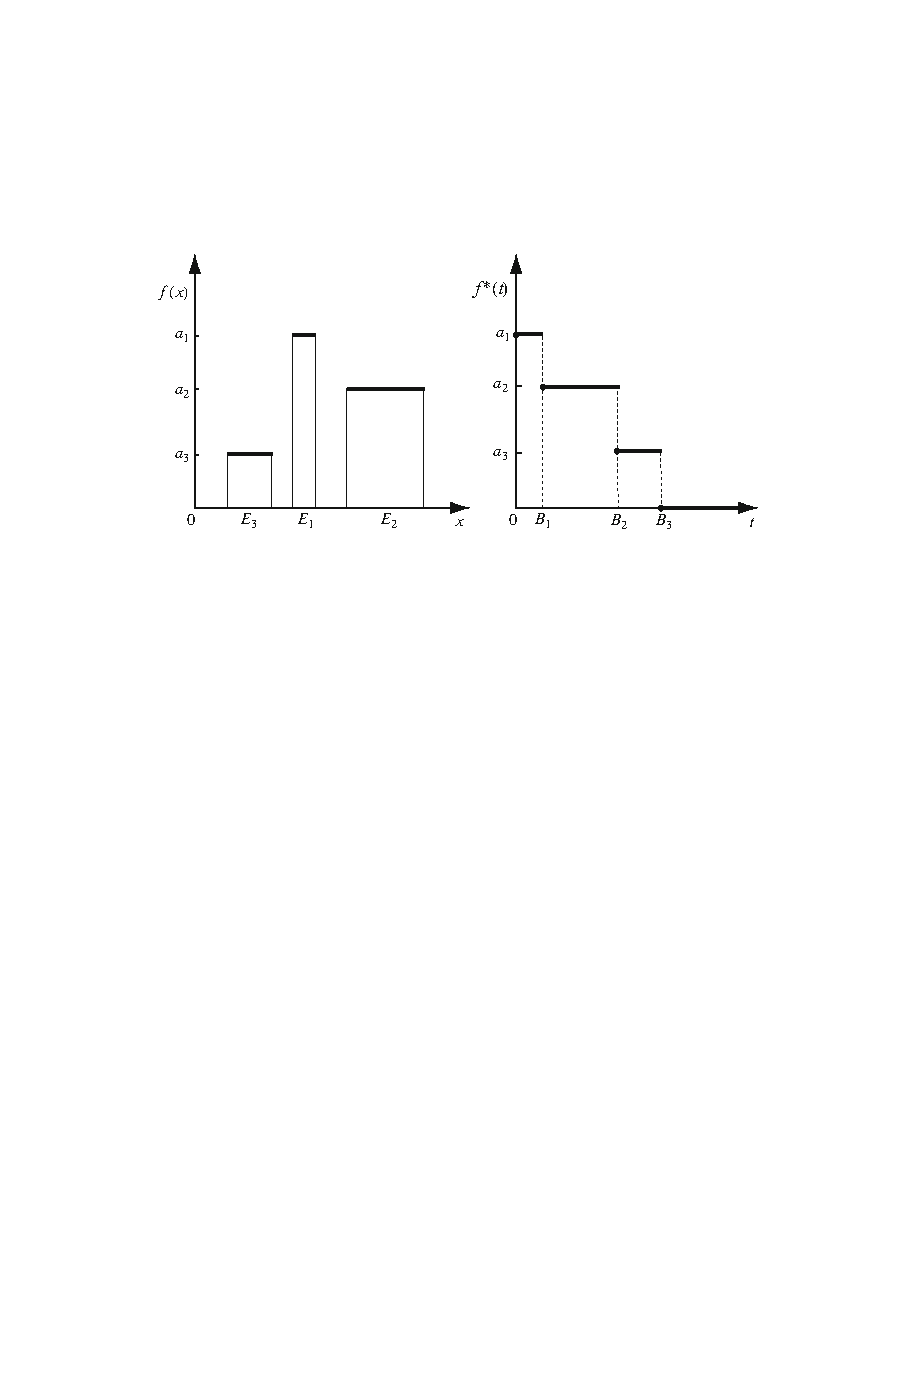
\includegraphics{pictures/rearrangement-of-simple}
\caption{The graph of a simple function and its decreasing rearrangement.}
\end{figure}
\begin{example}
Let $0<p<+\infty$. On $\R^n$ define $f$ by $f(x)=(1+|x|^p)^{-1}$. A computation shows that
\[\lambda_f(\alpha)=\begin{cases}
\omega_n(\alpha^{-1}-1)^{\frac{n}{p}}&\alpha<1,\\
0&\alpha\geq 1,
\end{cases}\quad\quad f^*(t)=\frac{1}{1+(t/\omega_n)^{\frac{p}{n}}},\]
where $\omega_n$ is the volume of the unit ball in $\R^n$.
\end{example}
\begin{example}
Again on $\R^n$ let $g(x)=1-e^{-|x|^2}$. We can easily see that $\lambda_g(\alpha)=0$ if $\alpha\geq 1$ and $\lambda_f(\alpha)=+\infty$ if $\alpha<1$. We conclude that $g^*(t)=1$ for all $t\geq 0$. This example indicates that although quantitative information is preserved, significant qualitative information is lost in passing from a function to its decreasing rearrangement.
\end{example}
The following are some properties of the function $f^*$.
\begin{proposition}\label{decreasing rearrangement prop}
Let $(X,\mathcal{A},\mu)$ be a measure space. Then we have
\begin{itemize}
\item[(a)] $f^*$ is right continuous and decreasing.
\item[(b)] $f^*(\lambda_f(\alpha))\leq\alpha$ for $\alpha>0$ and $\lambda_f(f^*(t))\leq t$ for $t>0$.
\item[(c)] $f^*(t)>\alpha$ if and only if $t<\lambda_f(\alpha)$.
\item[(d)] $f^*=|f|^*$, and $|f|\leq|g|$ $\mu$-a.e. implies that $f^*\leq g^*$.
\item[(e)] $(f+g)^*(t_1+t_2)\leq f^*(t_1)+g^*(t_2)$ and $(fg)^*(t_1t_2)\leq f^*(t_1)g^*(t_2)$.
\item[(f)] If $|f_n|$ increases to $|f|$, then $f_n^*$ increases to $f^*$, and $|f|\leq\varliminf_n|f_n|$ implies $f^*\leq\varliminf_nf_n^*$.
\item[(g)] $\lambda_f=\lambda_{f^*}$, i.e., $f$ and $f^*$ is equidistributed. 
\item[(h)] $(|f|^p)^*=(f^*)^p$ for $0<p<+\infty$.
\item[(i)] $\|f\|_p^p=\int_{0}^{+\infty}f^*(t)^p\,dt$ and $\|f\|_{+\infty}=f^*(0)$.
\item[(j)] $\sup_{t>0}tf^*(t)^p=\sup_{\alpha>0}\alpha^p\lambda_f(\alpha)$ for $0<p<+\infty$.   
\end{itemize}
\end{proposition}
\begin{proof}
Part $(a),(b),(c)$ are trivial from definition. For (d), if $|f|\leq|g|$, then by Proposition~\ref{distribution function prop} we have $\lambda_f\leq\lambda_g$, so it follows by definition that $f^*\leq g^*$.\par
Now we prove (e). Define
\[A=\{\alpha_1>0:\lambda_f(\alpha_1)\leq t_1\},\quad B=\{\alpha_2>0:\lambda_g(\alpha_2)\leq t_2\},\]
and
\[S=\{\alpha>0:\lambda_{f+g}(\alpha)\leq t_1+t_2\},\quad P=\{\alpha>0:\lambda_{fg}(\alpha)\leq t_1t_2\}.\]
Then by the properties of $\lambda_f$, we have $A+B\sub S$ and $AB\sub P$. Taking infimum then gives (e).\par
Now let $|f_n|$ increases to $f$. Then it follows from (d) that $f_n^*\leq f_{n+1}^*\leq f^*$ for all $n$. Let $h=\lim_nf_n^*$; then obviously $h\leq f^*$. Since $f_n^*\leq f^*$, we have
\[\lambda_{f_n}(h(t))\leq\lambda_{f_n}(f_n^*(t))\leq t,\]
which implies $\lambda_f(h(t))\leq t$ by letting $n\to+\infty$. It follows that $f^*(t)\leq h(t)$, hence $f^*=h^*$.\par
We prove (g). If $f$ is a simple function, then this is immediate in view of Examples~\ref{distribution of simple function} and \ref{decreasing rearrangement of simple}. For an arbitrary measurable function $f$, find a sequence of nonnegative simple functions $f_n$ such that $f_n$ increases to $|f|$. Then by (f) we have $f_n^*\to f^*$. Now if $|f|\leq\varliminf_n|f_n|$, set $F_n=\inf_{k\geq n}|f_k|$ and $h=\varliminf_n|f_n|=\sup_nF_n$. Since $F_n$ increases to $h$, by the previous argument we have $F_n^*$ increases to $h$. By hypothesis we have $|f|\leq h$, hence $f^*\leq h^*=\sup_nF_n^*$. Since $F_n\leq|f_k|$ for all $k\geq n$, we have $F_n^*\leq f_k^*$ for $k\geq n$, and hence $F_n^*\leq\varliminf_nf_n^*$. Putting these facts together, we obtain $f^*\leq h^*=\sup_n F_n^*\leq\varliminf_nf_n^*$. Thus (f) is proved.\par
For (h), just note that $\lambda_{|f|^p}(\alpha)=\lambda_f(\alpha^{1/p})$, and therefore
\begin{align*}
(|f|^p)^*(t)&=\inf\{\alpha>0:\lambda_{|f|^p}(\alpha)\leq t\}=\inf\{\alpha>0:\lambda_{|f|}(\alpha^{1/p})\leq t\}\\
&=\inf\{\alpha^p>0:\lambda_{|f|}(\alpha)\leq t\}=f^*(t)^{p}.
\end{align*}

Now, since $f$ and $f^*$ are equidistributed, by Proposition~\ref{L^p norm integral by distribution}, we have
\[\int|f|=\int_{0}^{+\infty}\lambda_{f}(\alpha)\,d\alpha=\int_{0}^{+\infty}\lambda_{f^*}(\alpha)\,d\alpha=\int_{0}^{+\infty}f^*(t)\,dt.\]
Thus by (h) we get
\[\|f\|_p^p=\int_{0}^{+\infty}(|f|^p)^*(t)\,dt=\int_{0}^{+\infty}f^*(t)^p\,dt.\]
Since $f^*(0)=\int\{\alpha>0:\lambda_f(\alpha)>0\}=\int\{\alpha>\mu(\{|f|>\alpha\})>0\}$, these together prove (i).\par
Finally, given $\alpha>0$, without loss of generality we may assume $\lambda_f(\alpha)>0$. Pick $\eps$ satisfying $0<\eps<\lambda_f(\alpha)$. Part (b) yields $f^*(\lambda_f(\alpha)-\eps)>\alpha$, which implies that
\[\sup_{t>0}tf^*(t)^p\geq (\lambda_f(\alpha)-\eps)f^*(\lambda_f(\alpha)-\eps)^p>(\lambda_f(\alpha)-\eps)\alpha^p.\]
We first let $\eps\to 0$ and then take the supremum over all $\alpha>0$ to obtain one direction in (j). Conversely, given $t>0$, assume without loss of generality that $f^*(t)>0$, and pick $\eps$ such that $0<\eps<f^*(t)$. Part (b) yields $\lambda_f(f^*(t)-\eps)>t$, which implies that
\[\sup_{\alpha>0}\alpha^p\lambda_f(\alpha)\geq(f^*(t)-\eps)^p\lambda_f(f^*(t)-\eps)>t(f^*(t)-\eps)^p\]
Similarly, letting $\eps\to 0$ and then take the supremum over all $t>0$, weobtain the opposite direction of (j).
\end{proof}
Having disposed of the basic properties of decreasing rearrangements of functions, we proceed with the definition of the Lorentz spaces. First, let's recall that a measruable function $f$ is in weak $L^p$ if and only if
\[\sup_{\alpha>0}\Phi(\alpha):=\sup_{\alpha>0}\alpha\lambda_f(\alpha)^{1/p}<+\infty.\]
This inequality can be restated by saying that the $L^\infty$ norm of $\Phi$ is finite. On the other hand, by Proposition~\ref{distribution integral prop} we have
\[\|f\|_p=\Big(\int_{0}^{+\infty}p\alpha^{p-1}\lambda_f(\alpha)\,d\alpha\Big)^{1/p}=\Big(p\int_{0}^{+\infty}\Phi(\alpha)^p\frac{d\alpha}{\alpha}\Big)^{1/p},\]
so $f\in L^p$ if and only if $\Phi$ is in $L^p((0,+\infty))$ with respect to the measure $pd\alpha/\alpha$. Now suppose that, instead of the $L^\infty$ norm or the $L^p$ norm of $\Phi$, we considered a $L^q$ norm, with $1\leq q<+\infty$; that is, we have
\begin{align}\label{Lorentz norm-1}
\Big(\int_{0}^{+\infty}p\Phi(\alpha)^q\frac{d\alpha}{\alpha}\Big)^{1/q}<+\infty.
\end{align}
This boundedness condition then lead us to the Lorentz spaces.\par
Before give the precise definition, let's first note that, the expression $(\ref{Lorentz norm-1})$ involves the function $\Phi$ and does not define a norm in general. However, there are other inequalities that are related to it that, in most cases, involve the finiteness of a norm. Recall that Proposition~\ref{decreasing rearrangement prop} tells us that
\[\sup_{t>0}t^{1/p}f^*(t)=\sup_{\alpha>0}\alpha\lambda_f(\alpha)^{1/p}=\sup_{\alpha>0}\Phi(\alpha).\]
The point is that we replace $\Phi(\alpha)$ by $t^{1/p}f^*(t)$ in $(\ref{Lorentz norm-1})$. That is, we consider the following boundedness condition:
\begin{align}\label{Lorentz norm-2}
\Big(\int_{0}^{+\infty}p(t^{1/p}f^*(t))^q\frac{dt}{t}\Big)^{1/q}<+\infty.
\end{align}
We are close to the definition of Lorentz spces, but we still need a small modification in $(\ref{Lorentz norm-2})$: if $q=p$, we want to return to the nrom of $L^p$ spaces. However, we know that
\begin{align}\label{Lorentz norm-3}
\|f\|_p=\Big(\int_{0}^{+\infty}f^*(t)^p\,dt\Big)^{1/p}.
\end{align}
Thus we make the following definition:
\begin{definition}
Let $(X,\mathcal{A},\mu)$ be a measure space and $f$ be a measurable function on $X$. $0<p\leq+\infty$. Let $0<p\leq+\infty$. For $0<q<+\infty$ we define
\[\|f\|_{p,q}=\Big(\int_{0}^{+\infty}(t^{1/p}f^*(t))^q\frac{dt}{t}\Big)^{1/q}\]
and we define the \textbf{Lorentz space} $L^{p,q}(X,\mathcal{A},\mu)$ to be the set of all $f$ such that $\|f\|_{p,q}<+\infty$. The space $L^{p,+\infty}(X,\mathcal{A},\mu)$ is defined to be the weak $L^p$ space. 
\end{definition}
As usual, two functions in $L^{p,q}(X,\mathcal{A},\mu)$ are considered equal if they are equal $\mu$-almost everywhere. By Proposition~\ref{decreasing rearrangement prop} we know that for $q=+\infty$ this definition coincides with the weak $L^p$ norm, and for $q=p$ we get $L^{p,p}(X,\mathcal{A},\mu)=L^p(X,\mathcal{A},\mu)$. Therefore Lorentz spaces can be viewed as a generalization of $L^p$ and weak $L^p$ spaces.
\begin{example}\label{L^pq norm for simple}
Using the notation of Example~\ref{decreasing rearrangement of simple}, when $0<p,q<+\infty$ we have
\[\|f\|_{p,q}=\Big(\frac{p}{q}\Big)^{1/q}\Big(a_1^qB_1^{\frac{q}{p}}+a_2^q[B_2^{\frac{q}{p}}-B_1^{\frac{q}{p}}]+\cdots+a_n^q[B_n^{\frac{q}{p}}-B_{n-1}^{\frac{q}{p}}]\Big)^{1/q},\]
and also $\|f\|_{p,+\infty}=\sup_{1\leq j\leq n}a_jB_j^{1/p}$. Next, we calculate $\|f\|_{+\infty,q}$ for the simple function $f$ of Example~\ref{decreasing rearrangement of simple}, where $qL+\infty$. It turns out that
\[\|f\|_{+\infty,q}=\Big(a_1^q\log\frac{B_1}{B_0}+a_2^q\frac{B_2}{B_1}+\cdots+a_n^q\frac{B_n}{B_{n-1}}\Big)^{1/q}.\]
Since $B_0=0$, we conclude that the only nonnegative simple function with finite $L^{+\infty,q}$ norm is the zero function. In fact, given a general nonzero function $g\in L^{+\infty,q}$ with $0<q<+\infty$, there is a nonzero simple function $\phi$ with $0\leq\phi\leq g$. Then $\phi$ has infinite norm, and therefore so does $g$. We deduce that $L^{+\infty,q}=\{0\}$ for $0<q<+\infty$.
\end{example}
\begin{proposition}
For $0<p,q<+\infty$, we have the identity
\begin{align}\label{L^pq norm equality}
\|f\|_{p,q}=\Big(p\int_{0}^{+\infty}[\alpha\lambda_f(\alpha)^{1/p}]^q\frac{d\alpha}{\alpha}\Big)^{1/q}.
\end{align}
\end{proposition}
\begin{proof}
If $f$ is the simple function of Example~\ref{decreasing rearrangement of simple}, then
\[\lambda_f(\alpha)=\sum_{j=0}^{n}B_j\chi_{[a_{j+1},a_j)}(\alpha),\]
with the understanding that $a_{n+1}=0$ and $a_0=+\infty$. Using the this formula and identity in Example~\ref{L^pq norm for simple}, we obtain the validity of $(\ref{L^pq norm equality})$ for simple functions. In general, given a measurable function $f$, find a sequence of nonnegative simple functions such that $f_n$ increases to $|f|$ a.e. Then $\lambda_{f_n}$ increases to $\lambda_f$ and $f_n^*$ increases to $f^*$. Using the Lebesgue monotone convergence theorem we deduce $(\ref{L^pq norm equality})$.
\end{proof}
Since $L^{p,p}\sub L^{p,+\infty}$, one may wonder whether these spaces are nested. The next result shows that for any fixed $p$, the Lorentz spaces $L^{p,q}$ increase as the exponent $q$ increases. Thus the space $L^{p,+\infty}$ can be viewed as the "biggest $L^p$ space".
\begin{proposition}
Suppose $0<p\leq+\infty$ and $0<q\leq r\leq+\infty$. Then there exists a constant $C_{p,q,r}$ (which depends on $p$, $q$, and $r$) such that
\begin{align}\label{L^pq inclusion}
\|f\|_{p,r}\leq C_{p,q,r}\|f\|_{p,q}.
\end{align}
In other words, $L^{p,q}$ is a subspace of $L^{p,r}$.
\end{proposition}
\begin{proof}
We may assume $p<+\infty$, since the case $p=+\infty$ is trivial. We have
\begin{align*}
t^{1/p}f^*(t)=\Big(\frac{q}{p}\int_{0}^{t}(s^{1/p}f^*(t))^q\frac{ds}{s}\Big)^{1/q}\leq \Big(\frac{q}{p}\int_{0}^{t}(s^{1/p}f^*(s))^q\frac{ds}{s}\Big)^{1/q}\leq\Big(\frac{q}{p}\Big)^{1/p}\|f\|_{p,q}.
\end{align*}
Hence, taking the supremum over all $t>0$, we obtain
\[\|f\|_{p,+\infty}\leq\Big(\frac{q}{p}\Big)^{1/q}\|f\|_{p,q}.\]
This establishes $(\ref{L^pq inclusion})$ in the case $r=+\infty$. Finally, when $r<+\infty$, we have
\[\|f\|_{p,r}=\Big(\int_{0}^{+\infty}(t^{1/p}f^*(t))^{r-q+q}\Big)^{1/r}\leq\|f\|_{p,+\infty}^{(r-q)/r}\|f\|_{p,q}^{q/r}\leq\Big(\frac{q}{p}\Big)^{\frac{r-q}{rq}}\|f\|_{p,q}.\]
This prves the claim.
\end{proof}
Unfortunately, the functionals $\|\cdot\|_{p,q}$ do not satisfy the triangle inequality. However, since for all $t>0$ we have $(f+g)^*(t)\leq f^*(t)+g^*(t)$, the estimate
\[\|f+g\|_{p,q}\leq 2^{\max\{\frac{1}{p},\frac{1}{p}+\frac{1-q}{q}\}}(\|f\|_{p,q}+\|g\|_{p,q})\]
holds. Also, if $\|f\|_{p,q}=0$, then we must have $f=0$ $\mu$-a.e. Therefore, $L^{p,q}$ is a quasi-normed space for all $p,q$ with $0<p,q\leq+\infty$. Is this space complete with respect to its quasi-norm? The next theorem answers this question.
\begin{theorem}
Let $(X,\mathcal{A},\mu)$ be a measure space. Then for all $0<p,q\leq+\infty$, the spaces $L^{p,q}(X,\mathcal{A},\mu)$ are complete with respect to their quasi-norm and they are therefore quasi-Banach spaces.
\end{theorem}
It is well known that finitely simple functions are dense in $L^p$ of any measure space, when $0<p<+\infty$. It is natural to ask whether finitely simple functions are also dense in $L^{p,q}$. This is in fact the case provided $q\neq+\infty$.
\begin{proposition}
Integrable simple functions are dense in $L^{p,q}$ for $0<q<+\infty$.
\end{proposition}
\begin{remark}
One may wonder whether simple functions are dense in $L^{p,+\infty}$. This
turns out to be false for all $0<p\leq+\infty$. However, countable linear combinations of characteristic functions of sets with finite measure are dense in $L^{p,+\infty}(X,\mathcal{A},\mu)$. We call such functions countably simple.
\end{remark}
\section{The Marcinkiewicz interpolation theorem, general form}
We now present the off-diagonal extension of Marcinkiewicz's interpolation theorem.
\begin{definition}
We say an operator $T$ is \textbf{restricted weak type $\bm{(p,q)}$}, if there exists $C\in(0,+\infty)$ such that for all $A\in\mathcal{A}$ with $\mu(A)<+\infty$, we have
\[\|T(\chi_A)\|_{q,+\infty}\leq C\|\chi_A\|_{p}=C\mu(A)^{1/p}.\]
In particular, if $T$ is weak type $(p,q)$, then it is also restricted weak type $(p,q)$.
\end{definition}
It is important to observe that if an operator is of restricted weak type $(p_0,q_0)$ and of restricted weak type $(p_1,q_1)$, then it is of restricted weak type $(p,q)$, where the indices are as in $(\ref{interpolation index})$ (This follows from Proposition~\ref{interpolation for weak norms-1}).
\begin{theorem}[\textbf{Marcinkiewicz Interpolation Theorem, General Form}]
Let $(X,\mathcal{A},\mu)$ and $(Y,\mathcal{B},\nu)$ be $\sigma$-finite measure spaces. Let $p_0,q_0,p_1,q_1\in(0,+\infty]$ are $T:(L^{p_0}+L^{p_1})(X,\mathcal{A},\mu)\to L^0(Y,\mathcal{B},\nu)$ be sublinear and for $t\in[0,1]$ define
\[p:=\frac{1-t}{p_0}+\frac{t}{p_1},\quad q:=\frac{1-t}{q_0}+\frac{t}{q_1}.\]
If there exist constants $C_0,C_1$ such that
\[\|T(\chi_A)\|_{q_0,+\infty}\leq C_0\mu(A)^{1/p_0},\quad \|T(\chi_A)\|_{q_1,+\infty}\leq C_1\mu(A)^{1/p_1},\]
then for any $r>0$, $t\in(0,1)$ and $f$ in $L^{p}(\mu)$ we have the estimate
\[\|Tf\|_{q,r}\leq C_t\|f\|_{p,r}.\]
In particular, if $p<q$, then $T$ is of strong type $(p,q)$. 
\end{theorem}
\begin{proposition}[\textbf{Schur test, extended version}]\label{Schur test extended}
Suppose $(X,\mathcal{A},\mu)$ and $(Y,\mathcal{B},\nu)$ are $\sigma$-finite measure spaces and let $K$ be a measurable function on $X\times Y$. Suppose that, for some $r,s\geq 1$,
\begin{align}\label{Schur test extended-1}
\exists C_1\in(0,+\infty):\quad \|K(x,\cdot)\|_{L^r(\nu)}\leq C_1\quad\text{for a.e. $x\in X$},
\end{align}
and
\begin{align}\label{Schur test extended-2}
\exists C_2\in(0,+\infty):\quad \|K(\cdot,y)\|_{L^s(\mu)}\leq C_2\quad\text{for a.e. $y\in Y$},
\end{align}
Then the operator defined by
\[Tf(x)=\int K(x,y)f(y)\,d\nu(y)\]
is strong type $(p,q)$ for every $p$ and $q$ with ($r'$ is the conjugate exponent of $r$)
\begin{align}\label{Schur test extended-3}
1\leq p\leq r',\quad s\leq q\leq+\infty,\quad \frac{1}{p}+\frac{1}{r}=1+\frac{s}{r}\cdot\frac{1}{q}.
\end{align}
\end{proposition}
\begin{proof}
First observe that, by H\"older's inequality we have
\[\|Tf\|_\infty\leq\int |K(x,y)f(y)|\,d\nu(y)\leq\|K(x,\cdot)\|_{L^r(\nu)}\|f\|_{r'}\leq C_1\|f\|_{r'}.\]
Thus $T$ is strong type $(r',+\infty)$. Moreover, Minkowski's integral inequality implies
\[\|Tf\|_{L^s(\mu)}=\Big\|\int K(x,y)f(y)\,d\nu(y)\Big\|_{L^s(\mu)}\leq\int\|K(x,y)f(y)\,d\mu(x)\|_{L^s(\mu)}\,d\nu(y)\leq C_2\|f\|_1,\]
and so $T$ is strong type $(1,s)$. Whenever there is $t\in[0,1]$ such that
\begin{align}\label{Schur test extended-4}
\frac{1}{p}=1-t+\frac{t}{r'}=1-\frac{t}{r},\quad\frac{1}{q}=\frac{1-t}{s},
\end{align}
Riesz-Thorin interpolation theorem implies that $T$ is strong type $(p,q)$. The condition $(\ref{Schur test extended-4})$ is now readily checked to be equivalent to $(\ref{Schur test extended-3})$.
\end{proof}
Using Marcinkiewicz interpolation instead of Riesz-Thorin's, we then get also a weak-type version of the Schur test:
\begin{proposition}[\textbf{Schur test, weak-type version}]\label{Schur test extended weak}
Let $(X,\mathcal{A},\mu)$ and $(Y,\mathcal{B},\nu)$ be $\sigma$-finite measure spaces and let $K$ be a measurable function on $X\times Y$. Suppose that, for some $r,s\geq 1$,
\begin{align}\label{Schur test extended weak-1}
\exists C_1\in(0,+\infty):\quad \|K(x,\cdot)\|_{L^{r,+\infty}(\nu)}\leq C_1\quad\text{for a.e. $x\in X$},
\end{align}
and
\begin{align}\label{Schur test extended weak-2}
\exists C_2\in(0,+\infty):\quad \|K(\cdot,y)\|_{L^{s,+\infty}(\mu)}\leq C_2\quad\text{for a.e. $y\in Y$},
\end{align}
Then the operator defined by
\[Tf(x)=\int K(x,y)f(y)\,d\nu(y)\]
is strong type $(p,q)$ for every $p$ and $q$ with ($r'$ is the conjugate exponent of $r$)
\begin{align}\label{Schur test extended weak-3}
1\leq p\leq r',\quad s\leq q\leq+\infty,\quad \frac{1}{p}+\frac{1}{r}=1+\frac{s}{r}\cdot\frac{1}{q}.
\end{align}
\end{proposition}
\begin{proof}
We start by noting that, for any $A\in\mathcal{A}$ with $\mu(A)<+\infty$, Tonelli's theorem shows along with the inequality (\ref{weak L^p normability and metrizability-1}) that
\begin{align*}
\int_A\Big|\int K(x,y)f(y)\,d\nu(y)\Big|\,d\mu(x)&\leq\int\Big(\int_A|K(x,y)|\,d\mu(x)\Big)\,|f(y)|\,d\nu(y)\\
&\leq\frac{sC_2}{s-1}\mu(A)^{1-1/s}\|f\|_{L^1(\nu)}.
\end{align*}
Thus Proposition~\ref{weak L^p normability and metrizability} implies that $\|Tf\|_{L^{s,+\infty}(\mu)}\leq\frac{sC_2}{s-1}\|f\|_{L^1(\nu)}$ and so $T$ is weak 
type $(1,s)$.\par
For the other "boundary" weak-type property, we note that for any $B\in\mathcal{B}$ with $\nu(B)<+\infty$,
\begin{align*}
|T\chi_B|&\leq\int|K(x,y)\chi_B(y)|\,d\nu(y)\leq\|f\|_{\infty}\int_{B}|K(x,y)|\,d\nu(y)\\
&\leq C_1\|f\|_\infty\nu(B)^{1-1/r}=C_1\|f\|_{\infty}\mu(B)^{1/r'}.
\end{align*}
Therefore $T$ is restricted weak type $(r',+\infty)$. This is sufficient for the Marcinkiewicz interpolation theorem and so $T$ is strong type $(p,q)$ for any $p$ and $q$ satisfying (\ref{Schur test extended weak-3}).
\end{proof}
\newpage
\chapter{Elements of Fourier analysis}
\section{Schwartz functions}
In this part we introduce the single most important tool in harmonic analysis, the Fourier transform. It is often the case that the Fourier transform is introduced as an operation on $L^1$ functions. In this exposition we first define the Fourier transform on a smaller class, the space of Schwartz functions, which turns out to be a very natural environment. Once the basic properties of the Fourier transform are derived, we extend its definition to other spaces of functions.\par
We begin with some preliminaries. Given $x=(x_1,,\dots,x_n)\in\R^n$, we set $|x|=(x_1^2+\cdots+x_n^2)^{1/2}$. The partial derivative of a function $f$ on $\R^n$ with respect to the $j$-th variable $x_j$ is denoted by $\partial_jf$ while the $k$-th partial derivative with respect to the $j$-th variable is denoted by $\partial_j^kf$. The gradient of a function $f$ is the vector $\nabla f=(\partial_1f,\dots,\partial_nf)$. A \textbf{multi-index} $\alpha$ is an ordered $n$-tuple of nonnegative integers. For a multi-index $\alpha=(\alpha_1,\dots,\alpha_n)$, $\partial^\alpha f$ denotes the derivative $\partial_1^{\alpha_1}\cdots\partial_n^{\alpha_n}f$. If $\alpha=(\alpha_1,\dots,\alpha_n)$ is a multi-index, $|\alpha|=\alpha_1+\cdots+\alpha_n$ denotes its size and $\alpha!=\alpha_1!\cdots\alpha_n!$ denotes the product of the factorials of its entries. The number $|\alpha|$ indicates the total order of differentiation of $\partial^\alpha f$.\par
For $x\in\R^n$ and $\alpha=(\alpha_1,\dots,\alpha_n)$ a multi-index, we set $x^\alpha=x_1^{\alpha_1}\cdots x_n^{\alpha_n}$. It is a simple fact to verify that
\begin{align}\label{multi-index inequality-1}
|x^\alpha|\leq c_{n,\alpha}|x|^{|\alpha|}
\end{align}
for all $x\in\R^n\setminus\{0\}$. In fact, $c_{n,\alpha}$ is the maximum of the continuous function $x\mapsto|x^\alpha|$ on the sphere $S^{n-1}$. The converse inequality in $(\ref{multi-index inequality-1})$ fails. However, the following substitution is of great use: for $k\in\Z^+$ we have
\begin{align}\label{multi-index inequality-2}
|x|^k\leq C_{n,k}\sum_{|\beta|=k}|x^\beta|
\end{align}
for all $x\in\R^n\setminus\{0\}$. To prove $(\ref{multi-index inequality-2})$, take $1/C_{n,k}$ to be the minimum of the function $x\mapsto\sum_{|\beta|=k}|x^\beta|$ on $S^{n-1}$; this minimum is positive since this function has no zeros on $S^{n-1}$. A related inequality is
\begin{align}\label{multi-index inequality-3}
(1+|x|)^k\leq 2^k(1+C_{n,k})\sum_{|\beta|=k}|x^\beta|.
\end{align}
This follows from $(\ref{multi-index inequality-2})$ for $|x|\geq 1$, while for $|x|<1$ we note that the sum in $(\ref{multi-index inequality-3})$ is at least one since $|x^{(0,\dots,0)}|=1$.\par
We end the preliminaries by the product rule for derivatives:
\[\partial^\alpha(fg)=\sum_{\beta\leq\alpha}\binom{\alpha}{\beta}(\partial^\beta f)(\partial^{\alpha-\beta}g).\]
for $f,g$ in $C^{|\alpha|}(\R^n)$ for some multi-index $\alpha$.\par
Two spaces of $C^\infty$ functions on $\R^n$ will be of particular importance for us. The first is the space $C_c^\infty$ of $C^\infty$ functions with compact support. The existence of nonzero functions in $C_c^\infty$ is not quite obvious; the standard construction is based on the fact that the function $\eta(x)=e^{-1/x}\chi_{(0,+\infty)}(t)$ is $C^\infty$ even at the origin. If we set $\psi(x)=\eta(1-|x|^2)$, then $\psi\in C_c^\infty(\R^n)$, and $\supp(\psi)$ is the closed unit ball. Later we shall use this single function to manufacture elements of $C_c^\infty$ in great profusion.\par
The other space of $C^\infty$ functions we shall need is the \textbf{Schwartz space}. Roughly speaking, a function is Schwartz if it is smooth and all of its derivatives decay faster than the reciprocal of any polynomial at infinity. More precisely, we give the following definition.
\begin{definition}
A $C^\infty$ function $f$ on $\R^n$ is called a \textbf{Schwartz function} if for every pair of multi-indices $\alpha$ and $\beta$ we have
\[\rho_{\alpha,\beta}(f)=\sup_{x\in\R^n}|x^\alpha\partial^\beta f(x)|<+\infty.\]
The quantities $\rho_{\alpha,\beta}(f)$ are called the \textbf{Schwartz seminorms} of $f$. The set of all Schwartz functions on $\R^n$ is denoted by $\mathscr{S}$.
\end{definition}
\begin{example}
The function $e^{-|x|^2}$ is in $\mathscr{S}$ but $e^{-|x|}$ is not, since it fails to be differentiable at the origin. The $C^\infty$ function $g(x)=(1+|x|^4)^{-a}$, $a>0$, is not in $\mathscr{S}$ since it decays only like the reciprocal of a fixed polynomial at infinity. The set of all smooth functions with compact support, $C_c^{\infty}(\R^n)$, is contained in $\mathscr{S}$.
\end{example}
\begin{example}
If $f_1$ is in $\mathscr{S}(\R^n)$ and $f_2$ is in $\mathscr{S}(\R^m)$, then the function $f_1f_2$ is in $\mathscr{S}(\R^{n+m})$. If $f$ is in $\mathscr{S}$ and $P(x)$ is a polynomial of $n$ variables, then $P(x)f(x)$ is also in $\mathscr{S}$. If $\alpha$ is a multi-index and $f$ is in $\mathscr{S}(\R^n)$, then $\partial^\alpha f$ is in $\mathscr{S}(\R^n)$. It is an important observation that if $f\in\mathscr{S}$ then $\partial^\alpha f\in L^p$ for all $\alpha$ and all $1\leq p\leq+\infty$. Indeed,  for all N,
\end{example}
Before proceeding, we prove a useful characterization for Schwartz functions.
\begin{proposition}\label{Schwarz space equivalent norm}
In the space $C^\infty(\R^n)$, the following are equivalent.
\begin{itemize}
\item[(\rmnum{1})] $|x^\alpha\partial^\beta f(x)|$ is bounded for all multi-indices $\alpha,\beta$.
\item[(\rmnum{2})] $|\partial^\alpha(x^\beta f)|$ is bounded for all multi-indices $\alpha,\beta$.
\item[(\rmnum{3})] $(1+|x|)^N|\partial^\alpha f(x)|$ is bounded for all multi-index $\alpha$ and $N>0$.
\end{itemize}
Therefore, either of the quantities above can be used to define the Schwartz space.
\end{proposition}
\begin{proof}
The equivalence of (\rmnum{1}) and (\rmnum{3}) is given by the inequalities $(\ref{multi-index inequality-3})$ and $|x^\alpha|\leq(1+|x|)^{|\alpha|}$. The second one follows from the fact that each $\partial^\alpha(x^\beta f)$ is a linear combination of terms of the form $x^\gamma\partial^\delta f$ and vice versa, by the product rule.
\end{proof}
Note that if $f\in\mathscr{S}$, then Proposition~\ref{Schwarz space equivalent norm} implies that $|\partial^\alpha f(x)|\leq C_N(1+|x|)^{-N}$ for all $N$. Since $(1+|x|)^{-N}$ is in $L^p$ for $N>p/n$, this implies $f\in L^p$ for all $1\leq p\leq+\infty$.\par
Now we investigate the property of Schwartz space.
\begin{proposition}
$\mathscr{S}$ is a Fr\'echet space with the topology defined by the norms $\rho_{\alpha,\beta}$.
\end{proposition}
\begin{proof}
The only nontrivial point is completeness. We make use of the norm
\[\|f\|_{(N,\alpha)}:=\sup_{x\in\R^n}(1+|x|)^{N}\partial^\alpha f(x)|.\]
(We note that this family of seminorms is equivalent to $\rho_{\alpha,\beta}$'s by Proposition~\ref{Schwarz space equivalent norm}, so we will fix this notation henceforth.) If $\{f_k\}$ is a Cauchy sequence in $\mathscr{S}$, then $\|f_i-f_j\|_{N,\alpha}\to 0$ for all $\alpha,\beta$. In particular, for each $\alpha$ the sequence $\{\partial^\alpha f_k\}$ converges uniformly to a function $g_\alpha$. Denoting by $e_j$ the vector $(0,\dots,1,\dots,0)$ with the $1$ in the $j$-th position, we have
\begin{align*}
f_k(x+te_j)-f_k(x)=\int_{0}^{t}\partial_jf_k(x+se_j)\,ds.
\end{align*}
Letting $n\to+\infty$, we get
\[g_0(x+te_j)-g_0(x)=\int_{0}^{t}g_{e_j}(x+se_j)\,ds.\]
The fundamental theorem of calculus implies that $g_{e_j}=\partial_jg_0$, and an induction on $|\alpha|$ then yields $g_\alpha=\partial^\alpha g_0$ for all $\alpha$. It is then easy to check that $\|f_k-g_0\|\to 0$ for all $\alpha$.
\end{proof}
We note that convergence in $\mathscr{S}$ is stronger than convergence in all $L^p$. We have the following.
\begin{proposition}\label{Schwarz converge stronger than L^p}
Let $\{f_k\}$ and $f$ be in $\mathscr{S}$ and $f_k\to f$ in $\mathscr{S}$. Then $f_k\to f$ in $L^p$ for all $0<p\leq+\infty$. Moreover, there exists a $C_{p,n}>0$ such that
\begin{align}\label{Schwarz converge stronger than L^p-1}
\|\partial^\beta f\|_{p}\leq C_{p,n}\sum_{|\alpha|\leq[\frac{n+1}{p}]+1}\rho_{\alpha,\beta}(f)
\end{align}
for all $f$ for which the right-hand side is finite.
\end{proposition}
\begin{proof}
Observe that when $p<+\infty$ we have
\begin{align*}
\|\partial^\beta f\|_{p}&\leq\Big[\int(\partial^\beta f(x))^p\,dx\Big]^{1/p}=\Big[\int_{|x|\leq 1}(\partial^\beta f(x))^p\,dx\Big]^{1/p}+\Big[\int_{|x|>1}(\partial^\beta f(x))^p\,dx\Big]^{1/p}\\
&\leq\Big[\omega_n\|\partial^\beta f\|_{\infty}^p+\sup_{|x|>1}|x|^{n+1}|\partial^\beta f(x)|^p\int_{|x|>1}|x|^{-(n+1)}\,dx\Big]^{1/p}\\
&\leq C_{p,n}\Big(\|\partial^\beta f\|_{\infty}+\sup_{|x|>1}|x|^{\frac{n+1}{p}}|\partial^\beta f(x)|\Big).
\end{align*}
The preceding inequality is also trivially valid when $p=+\infty$. Now set $m=(n+1)/p$ and use $(\ref{multi-index inequality-2})$ to obtain
\[\sup_{|x|>1}|x|^{m}|\partial^\beta f(x)|\leq\sup_{|x|>1}C_{n,m}\sum_{|\alpha|=m}|x^\alpha\partial^\beta f(x)|\leq C_{n,m}\sum_{|\alpha|\leq m}\rho_{\alpha,\beta}(f).\]
The claim now follows immediately.
\end{proof}
To end this part, we investigate the continuity of translations on various function spaces. The following notation for translations will be used throughout this section and the next one: If $f$ is a function on $\R^n$ and $y\in\R^n$,
\[\tau_yf(x)=f(x-y).\]
We observe that $\|\tau_yf\|_p=\|f\|_p$ for $1\leq p\leq +\infty$. A function $f$ is called uniformly continuous if $\|\tau_yf-f\|_{\infty}\to 0$ as $y\to 0$.
\begin{lemma}
If $f\in C_c(\R^n)$, then $f$ is uniformly continuous.
\end{lemma}
\begin{proposition}\label{L^p translation continuous}
For $1\leq p<+\infty$, translation is continuous in the $L^p$ norm; that is, if $f\in L^p$ and $z\in\R^n$, then $\lim_{y\to 0}\|\tau_{y+z}f-\tau_zf\|_p=0$.
\end{proposition}
\begin{proof}
Since $\tau_{y+z}=\tau_y\tau_z$, by replacing $f$ by $\tau_zf$ it suffices to assume that $z=0$. First, if $g\in C_c$, for $|y|\leq 1$ the functions $\tau_yg$ are all supported in a common compact set $K$, so
\[\int|\tau_yg-g|^p\leq\|\tau_yg-g\|_{\infty}^p\lambda(K)\to 0.\]
Now suppose $f\in L^p$. If $\eps>0$, by Proposition~\ref{Radon C_c(X) dense in L^p} there exists $g\in C_c$ such that $\|g-f\|<\eps/3$, so
\[\|\tau_yf-f\|_p\leq\|\tau_y(f-g)\|_p+\|\tau_yg-g\|_p+\|f-g\|_p<2\eps/3+\|\tau_yg-g\|_p.\]
and $\|\tau_yg-g\|_p<\eps/3$ if $y$ is sufficiently small.
\end{proof}
Proposition~\ref{L^p translation continuous} is false for $p=\infty$, as one should expect since the $L_\infty$ norm is closely related to the uniform norm.\par
Some of our results will concern multiply periodic functions in $\R^n$, and for simplicity we shall take the fundamental period in each variable to be $1$. That is, we define a function $f$ on $\R^n$ to be periodic if $f(x+k)=f(x)$ for all $x\in\R^n$ and $k\in\Z^n$. Every periodic function is thus completely determined by its values on the unit cube $Q=[-1/2,1/2)^n$. Periodic functions may be regarded as functions on the space $\R^n/\Z^n=(\R/\Z)^n$ of cosets of $\Z^n$, which we call the $n$-dimensional torus and denote by $\T^n$. Note that $\T^n$ is a compact Hausdorff space; it may be identified with the set of all $z=(z_1,\dots,z_n)\in\C^n$ such that $|z_j|=1$ for all $j$ via the map
\[(x_1,\dots,x_n)\mapsto(e^{2\pi ix_1},\dots,e^{2\pi ix_n}).\]
On the other hand, for measure-theoretic purposes we identify $\T^n$ with the unit cube $Q$, and when we speak of Lebesgue measure on $\T^n$ we mean the measure induced on $\T^n$ by Lebesgue measure on $Q$. In particular, $\lambda(\T^n)=1$. Functions on $\T^n$ may be considered as periodic functions on $\R^n$ or as functions on $Q$; the point of view will be clear from the context when it matters.
\section{Convolutions}
Let $f$ and $g$ be measurable functions on $\R^n$. The convolution of $f$ and $g$ is the function $f\ast g$ defined by
\[f\ast g=\int f(x-y)g(y)\,dy.\]
for all $x$ such that the integral exists. Various conditions can be imposed on $f$ and $g$ to guarantee that $f\ast g$ is defined at least almost everywhere. For example, if $f$ is bounded and compactly supported, $g$ can be any locally integrable function.\par
In what follows, we shall need the fact that if $f$ is a measurable function on $\R^n$, then the function $K(x,y)=f(x-y)$ is measurable on $\R^n\times\R^n$. We have $K=f\circ s$ where $s(x,y)=x-y$; since $s$ is continuous, $K$ is Borel measurable if $f$ is Borel measurable. This can always be assumed without affecting the definition of $f\ast g$, by Proposition~\ref{measurable extended value function completion}. However, the Lebesgue measurability of $K$ also follows from the Lebesgue measurability of $f$.\par
The elementary properties of convolutions are summarized in the following proposition.
\begin{proposition}\label{convolution on R^n prop}
Assuming that all integrals exist, we have
\begin{itemize}
\item[(a)] $f\ast g=g\ast f$.
\item[(b)] $(f\ast g)\ast h=f\ast(g\ast h)$.
\item[(c)] For $z\in\R^n$, $\tau_z(f\ast g)=(\tau_zf\ast g)=f\ast(\tau_zg)$.
\item[(d)] $\supp(f\ast g)\sub\overline{\supp(f)+\supp(g)}$.
\end{itemize}
\end{proposition}
\begin{proof}
Part (a) and (b) follows from the general properties of convolution on locally compact groups. So we only prove (c) and (d). For (c),
\begin{align*}
\tau_z(f\ast g)=\int f(x-z-y)g(y)\,dy=\int\tau_{z}f(x-y)g(y)\,dy=(\tau_zf)\ast g,
\end{align*}
and by (a),
\[\tau_z(f\ast g)=\tau_z(g\ast f)=(\tau_zg)\ast f=f\ast(\tau_zg).\]
For (d), we observe that if $x\notin\supp(f)+\supp(g)$, then for any $y\in\supp(g)$ we have $x-y\notin\supp(f)$, hence $f(x-y)g(y)=0$ for all $y$, so $f\ast g(x)=0$.
\end{proof}
The following two propositions contain the basic facts about convolutions of $L^p$ functions.
\begin{proposition}[\textbf{Minkowski's inequality}]
Let $1\leq p\leq+\infty$. If $f\in L^1$ and $g\in L^p$, then $f\ast g(x)$ exists for almost every $x$ and $f\ast g\in L^p$. Moreover,
\[\|f\ast g\|_p\leq\|f\|_1\|g\|_p.\]
\end{proposition}
\begin{proof}
This is a special case for Proposition~\ref{Schur test} with $K(x,y)=f(x-y)$.
\end{proof}
\begin{proposition}
If $p$ and $q$ are conjugate exponents, $f\in L^p$, and $g\in L^q$, then $f\ast g(x)$ exists for every $x$, $f\ast g$ is bounded and uniformly continuous, and $\|f\ast g\|_{\infty}\leq\|f\|_p\|g\|_q$. If $1<p<+\infty$, then $f\ast g\in C_0(\R^n)$.
\end{proposition}
\begin{proof}
The existence of $f\ast g$ and the estimate for $\|f\ast g\|_{\infty}$ follow immediately from Holder's inequality. In view of Propositions~\ref{L^p translation continuous}, so does the uniform continuity of $f\ast g$. In fact, if $1\leq p<+\infty$,
\[\|\tau_y(f\ast g)-f\ast g\|_{\infty}=\|(\tau_yf-f)\ast g\|_{\infty}\leq\|\tau_yf-f\|_p\|g\|_q\to 0.\]
And for $p=+\infty$, interchange the roles of $f$ and $g$. Finally, if $1<p,q<+\infty$, choose sequences $\{f_k\}$ and $\{g_k\}$ of functions with compact support such that $\|f_k-f\|_p\to 0$ and $\|g_k-g\|_q\to 0$. By Proposition~\ref{convolution on R^n prop} and what we have just proved, $f_k\ast g_k\in C_c$. But
\[\|f_k\ast g_k-f\ast g\|_\infty\leq\|f_k-f\|_p\|g_k\|_q+\|f\|_p\|g_k-g\|_q\to 0,\]
so $f\ast g\in C_0$ by Proposition~\ref{LCH C_0(X) is closure of C_c(X)}.
\end{proof}
The preceding results are all we shall use, but for the sake of completeness we state also the following generalization .
\begin{proposition}[\textbf{Young's inequality}]
Suppose $1\leq p,q,r\leq+\infty$ and $p^{-1}+q^{-1}=1+r^{-1}$.
\begin{itemize}
\item[(a)] If $f\in L^p$ and $g\in L^p$, then $f\ast g(x)$ exists for almost every $x$, and $f\ast g\in L^r$. Moreover, $\|f\ast g\|_r\leq\|f\|_p\|g\|_q$.
\item[(b)] Suppose that $1<p,q,r<+\infty$. If $f\in L^p$ and $g\in L^{q,+\infty}$, then $f\ast g\in L^r$ and $\|f\ast g\|_r\leq C_{p,q}\|f\|_p\|g\|_{q,+\infty}$ where $C_{p,q}$ is independent of $f$ and $g$.
\item[(c)] Suppose that $p=1$ and $r=q>1$. If $f\in L^1$ and $g\in L^{q,+\infty}$, then $f\ast g\in L^{q,+\infty}$ and $\|f\ast g\|_{q,+\infty}\leq C_q\|f\|_1\|g\|_{q,+\infty}$ where $C_q$ is independent of $f$ and $g$. 
\end{itemize}
\end{proposition}
\begin{proof}
To prove (a), let $q$ be fixed. The special cases $p=1$, $r=q$ and $p=q/(q-1)$, $r=+\infty$ are proved above. The general case then follows from the Riesz-Thorin interpolation theorem. Part (b) and (c) are special case of Proposition~\ref{Schur test extended weak}.
\end{proof}
One of the most important properties of convolution is that, roughly speaking, $f\ast g$ is at least as smooth as either $f$ or $g$, because formally we have
\[\partial^\alpha(f\ast g)=\partial^\alpha\int f(x-y)g(y)\,dy=\int\partial^\alpha f(x-y)d(y)\,dy=(\partial^\alpha f)\ast g.\]
and similarly $\partial^\alpha(f\ast g)=f\ast(\partial^\alpha g)$. To make this precise, one needs only to impose conditions on $f$ and $g$ so that differentiation under the integral sign is legitimate. One such result is the following.
\begin{proposition}\label{convolution on R^n derivative}
If $f\in L^1$, $g\in C^k$, and $\partial^\alpha g$ is bounded for $|\alpha|\leq k$, then $f\ast g\in C^k$ and $\partial^\alpha(f\ast g)=f\ast(\partial^\alpha g)$ for $|\alpha|\leq k$.
\end{proposition}
\begin{proof}
This is clear from Theorem~\ref{int change derivative and limit}.
\end{proof}
\begin{proposition}
Let $f,g$ be in $\mathscr{S}$. Then $f\ast g$ is in $\mathscr{S}$. Moreover,
\[\partial^\alpha(f\ast g)=(\partial^\alpha f)\ast g=f\ast(\partial^\alpha g)\]
for all multi-indices $\alpha$.
\end{proposition}
\begin{proof}
First, $f\ast g\in C^\infty$ by Proposition~\ref{convolution on R^n derivative}. Since
\begin{align}\label{convolution on schwarz}
1+|x|\leq 1+|x-y|+|y|\leq (1+|x-y|)(1+|y|),
\end{align}
we have
\begin{align*}
(1+|x|)^{N}|\partial^\alpha(f\ast g)(x)|&\leq\int (1+|x-y|)^N|\partial^\alpha(x-y)|(1+|y|)^N|g(y)|\,dy\\
&\leq\|f\|_{(N,\alpha)}\|g\|_{(N+n+1,\alpha)}\int(1+|y|)^{-n-1}\,dy<+\infty.
\end{align*}
Thus the claim follows.
\end{proof}
Convolutions of functions on the torus $\T^n$ are defined just as for functions on $\R^n$. (If one regards functions on $\T^n$ as periodic functions on $\R^n$, of course, the integration is to be extended over the unit cube rather than $\R^n$.) All of the preceding results remain valid, with the same proofs.\par
We now introduce the notion of approximate identities. By Young's inequality we have $\|f\ast g\|_1\leq\|f\|_1\|g\|_1$ for $f,g\in L^1(\R^n)$, so the space $L^1(\R^n)$ becomes a Banach algebra under convolution. However, $L^1(\R^n)$ may not have a unit element, that is, an element $f$ such that
\[f\ast g=g\ast g=g\quad\forall g\in L^1(\R^n).\]
This problem is resolved by a limiting process, which is called an approximate idnetity.
\begin{definition}
An \textbf{approximate identity} is a family of $L^1(\R^n)$ functions $\{\Phi_t\}_{t>0}$ with the following three properties:
\begin{itemize}
\item[(\rmnum{1})] There exists a constant $C>0$ such that $\|\Phi_t\|_1\leq C$ for all $t>0$.
\item[(\rmnum{2})] $\int\Phi_t(x)\,dx=1$ for all $t>0$.
\item[(\rmnum{3})] For any neighborhood $U$ of zero in $\R^n$ we have
\[\lim_{t\to 0}\int_{U^c}|\Phi_t(x)|\,dx=0.\] 
\end{itemize}
\end{definition}
Sometimes we think of approximate identities as sequences $\{\Phi_n\}_n$. In this case property (\rmnum{3}) holds as $n\to+\infty$. It is best to visualize approximate identities as a family of functions $\Phi_t(x)$ that spike near $0$ in such a way that the signed area under the graph of each function remains constant (equal to one) but the support shrinks to zero.
\begin{example}
On $\R$ consider the functions
\[P(x)=\frac{1}{\pi(1+x^2)},\quad P_t(x)=t^{-1}P(t^{-1}x).\]
Then $P_t$ and $P$ have the same $L^1$ norm and $\int P(x)\,dx=1$. Moreover, for any $\delta>0$, we have
\[\int_{|x|\geq\delta}P_t(x)\,dx=1-\frac{2}{\pi}\arctan\frac{\delta}{t}\to 0.\]
Thus the family $\{P_t\}$ is a approximate identity on $\R$.
\end{example}
The above example can be generalized: If $\phi$ is any function on $\R^n$ and $t>0$, we set
\[\phi_t(x)=t^{-n}\phi(t^{-1}x).\]
We observe that if $\phi\in L^1$, then $\int\phi_t=\int\phi$ for all $t$, and $\|\phi_t\|_1=\|\phi\|$. Moreover, for any $\delta>0$ we have
\[\lim_{t\to 0}\int_{|x|\geq\delta}\phi_t(x)\,dx=\lim_{t\to 0}\int_{|x|\geq\delta/t}\phi(x)\,dx=0.\]
Thus $\{\phi_t\}$ satisfies the conditions (\rmnum{1}) and (\rmnum{3}). If additionally $\int\phi=1$, then $\{\phi_t\}$ will become an approximate identity.\par
Now we establish the following basis property for approximate identity.
\begin{theorem}\label{convolution approximate identity in L^p}
Let $\{\Phi_t\}$ be an approximate identity on $\R^n$.
\begin{itemize}
\item[(a)] If $f\in L^p$ with $1\leq p<+\infty$, then $f\ast\Phi_t\to f$ in the $L^p$ norm as $t\to 0$.
\item[(b)] If $f$ is bounded and uniformly continuous, then $f\ast\Phi_t\to f$ uniformly as $t\to 0$.
\item[(c)] If $f\in L^\infty$ and $f$ is continuous on an open set $U$, then $f\ast\Phi_t\to f$ uniformly on compact subsets of $U$ as $t\to 0$.
\end{itemize}
\end{theorem}
\begin{proof}
We start by (a). Let $f\in L^p(\R^n)$, then by Proposition~\ref{L^p translation continuous}, we have $\lim_{y\to 0}\|\tau_yf-f\|_p=0$, thus for any fixed $\eps>0$, there exists $\delta>0$ such that $\|\tau_yf-f\|_p<\eps$. Since $\Phi_t$ has total integral $1$, we have
\begin{align*}
f\ast\Phi_t(x)-f(x)&=\int[f(x-y)-f(x)]\Phi_t(y)\,dy=\Big(\int_{|y|<\delta}+\int_{|y|\geq\delta}\Big)[f_y(x)-f(x)]\Phi_t(y)\,dy.
\end{align*}
Now take $L^p$ norm. By Minkowski's inequality for integrals, we have
\begin{align*}
\Big\|\int_{|y|<\delta}[f(x-y)-f(x)]\Phi_t(y)\,dy\Big\|_p\leq\int_{|y|<\delta}\|\tau_yf-f\|_p|\Phi_t(y)|\,dy<\eps\int_{|y|<\delta}|\Phi_t(y)|\,dy\leq C\eps.
\end{align*}
where $C=\sup_t\|\Phi_t\|_1$. On the other hand,
\begin{equation*}\small
\begin{aligned}
\Big\|\int_{|y|\geq\delta}[f(x-y)-f(x)]\Phi_t(y)\,dy\Big\|_p\leq\int_{|y|\geq\delta}\|f(\cdot-y)-f\|_p|\Phi_t(y)|\,dy\leq 2\|f\|_p\int_{|y|\geq\delta}|\Phi_t(y)|\,dy\to 0,
\end{aligned}
\end{equation*}
Thus part (a) follows. The proof of (b) is exactly the same, with $\|\cdot\|_p$ replaced by $\|\cdot\|_{\infty}$, and $\|\tau_{y}f-f\|_\infty\to 0$ as $y\to 0$ by the uniform continuity of $f$.\par
As for (c), assume that $f$ is continuous on $U$ and $K\sub U$ is compact. Then for fix $\eps>0$, by the compactness of $K$, there exists $\delta>0$ such that
\[\sup_{x\in K,|y|<\delta}|f(x-y)-f(x)|<\eps.\]
But then
\begin{align*}
\sup_{x\in K}|f\ast\Phi_t(x)-f(x)|&\leq\sup_{x\in K}\Big(\int_{|y|<\delta}+\int_{|y|>\delta}\Big)|f(x-y)-f(x)||\Phi_t(y)|\,dz\\
&\leq\eps\|\Phi_t\|_1+2\|f\|_\infty\int_{|y|\geq\eps}|\Phi_t(y)|\,dy
\end{align*}
from which (c) follows.
\end{proof}
The most common application for Theorem~\ref{convolution approximate identity in L^p} lies on the approximate identify $\{\phi_t\}$ induced by a $L^1$ function $\phi$. In this case, we can obtain the pointwise convergence for $f\ast\phi_t$ provided we add some extra condition on $\phi$.
\begin{definition}
For each $\phi\in L^1(\R^n)$, the \textbf{radical majorant} of $\phi$ is defined by
\[R_\phi(x)=\mathrm{ess.sup}\{|\phi(y)|:|y|\geq|x|\},\]
and let $\{\phi_t\}$ be the approximate identity on $\R^n$ induced by $\phi$.
\end{definition}
\begin{theorem}\label{convolution approximate identity a.e.}
Let $\phi\in L^1(\R^n)$ with $\int\phi(x)\,dx=a$. If $R_\phi\in L^1(\R^n)$, then for $1\leq p\leq+\infty$ and any $f\in L^p$, $f\ast\phi_t(x)\to af(x)$ as $t\to 0$ for every $x$ in the Lebesgue set of $f$ (in particular, for almost every $x$, and for every $x$ at which $f$ is continuous).
\end{theorem}
\begin{proof}
We may concentrate on the case $a=1$. If $x$ is in the Lebesgue set of $f$, for any $\delta>0$ there exists $\eta>0$ such that
\begin{align}\label{convolution approximate identity-1}
\int_{|y|<r}|f(x-y)-f(x)|\,dy\leq\delta r^n\for r\leq\eta.
\end{align}
To prove the claim $f\ast\phi_t(x)\to f(x)$, we need to estimate the integrals
\[I_1=\int_{|y|<\eta}|f(x-y)-f(x)||\phi_t(y)|\,dy,\quad I_2=\int_{|y|\geq\eta}|f(x-y)-f(x)||\phi_t(y)|\,dy.\]
We first observe that the function $R_\phi$ is radical and, if we put $R_\phi(x)=\varphi(|x|)$, then the function $\varphi$ is decreasing. Thus, if $\omega_n$ is the volume of the unit ball in $\R^n$, we have
\[\frac{\omega_n(2^n-1)}{2^n}r^n\varphi(r)\leq\int_{r/2\leq|x|\leq r}R_\phi(x)\,dx\to 0\]
as $r\to 0$ or $r\to+\infty$. In particular, there exists $C>0$ such that $r^n\varphi(r)\leq A$ for all $0\leq r<+\infty$. If we set $g(r)=\int_{S^{n-1}}|f(x-r\theta)-f(x)|\,d\theta$, then $(\ref{convolution approximate identity-1})$ is equivalent to
\[G(r)=\int_{0}^{r}s^{n-1}g(s)\,ds\leq\delta r^n\for r\leq\eta.\]
Using this observation and integration by parts, we have
\begin{equation*}
\begin{aligned}
I_1&\leq\int_{|y|<\eta}|f(x-y)-f(x)||t^{-n}R_\phi(y/t)|\,dy=\int_{0}^{\eta}r^{n-1}g(r)t^{-n}\varphi(r/t)\,dr\\
&=G(r)t^{-n}\varphi(r/t)\Big|_0^{\eta}-\int_{0}^{\eta}G(r)\,d(t^{-n}\varphi(r/t))=G(\eta)t^{-n}\varphi(\eta/t)-\int_{0}^{\eta/t}G(ts)t^{-n}\,d\varphi(s)\\
&\leq\delta\eta^nt^{-n}\varphi(\eta/t)-\int_{0}^{\eta/t}\delta s^n\,d\varphi(s)\leq\delta C-\delta\int_{0}^{+\infty}s^n\,d\varphi(s)=\delta C+n\delta\int_{0}^{+\infty}s^{n-1}\varphi(s)\,ds\\
&=\delta\Big(C+\omega_n^{-1}\int_{\R^n}\varphi(y)\,dy\Big).
\end{aligned}
\end{equation*}
As for $I_2$, if $q$ is the conjugate exponent to $p$ and $\chi_\eta$ is the characteristic function of $\{y:|y|\geq\eta\}$, by H\"older's inequality we have
\begin{align*}
I_2\leq \int_{|y|\geq\eta}(|f(x-y)|+|f(x)|)|\phi_t(y)|\,dy=\|f\|_p\|\chi_\eta\phi_t\|_q+|f(x)|\|\chi_\eta\phi_t\|_1,
\end{align*}
so it suffices to show that for $1\leq q\leq +\infty$, $\|\chi_\eta\phi_t\|_q\to 0$ for $t\to 0$. The case $q=1$ and $q=+\infty$ are easy to see
\[\|\chi_\eta\phi_t\|_\infty=\sup_{|y|\geq\eta}|\phi_t(y)|\leq\eta^{-n}(\eta/t)^n\varphi(|\eta/t|)\to 0,\]
and
\begin{equation*}
\begin{aligned}
\|\chi_\eta\phi_t\|_1&=\int_{|y|\geq\eta}t^{-n}|\phi(t^{-1}y)|\,dy=\int_{|z|\geq\eta/t}|\phi(z)|\,dz\leq\int_{|z|\geq\eta/t}R_\phi(z)\,dz\to 0,
\end{aligned}
\end{equation*}
so the general case follows from Proposition~\ref{L^p space intersection inequality}. This finishes the proof.
\end{proof}
\begin{corollary}
If $\phi\in L^1(\R^n)$ and there exists a nonnegative function $\Phi\in L^1(\R)$ such that $|\phi(x)|\leq\Phi(|x|)$ holds almost everywhere, then $\{\phi_t\}$ satisfies the conclusion of Theorem~\ref{convolution approximate identity a.e.}.
\end{corollary}
We now apply Theorem~\ref{convolution approximate identity in L^p} and \ref{convolution approximate identity a.e.} to prove some approximation results on functions in $L^p(\R^n)$.
\begin{proposition}\label{smooth compact function dense in L^p}
For $1\leq p<+\infty$, the space $C^\infty_c(\R^n)$ (and hence $\mathscr{S}$) is dense in $L^p(\R^n)$ and in $C_0(\R^n)$.
\end{proposition}
\begin{proof}
Given $f\in L^p$ and $\eps>0$, there exists $g\in C_c$ with $\|f-g\|_p<\eps/2$ by Proposition~\ref{Radon C_c(X) dense in L^p}. Let $\phi$ be a function in $C_c^\infty$ such that $\int\phi=1$ (for example, take $\phi=(\int\psi)^{-1}\psi$ where $\psi$ is a nonzero function in $C^\infty_c$). Then $g\ast\phi_t\in C_c^\infty$ by Propositions~\ref{convolution on R^n prop}(d) and \ref{convolution on R^n derivative}, and $\|g\ast\phi_t-g\|_p<\eps/2$ for sufficiently small $t$ by Theorem~\ref{convolution approximate identity a.e.}. The same argument applies if $L^p$ is replaced by $C_0$, $\|\cdot\|_p$ by $\|\cdot\|_\infty$, and Proposition~\ref{Radon C_c(X) dense in L^p} by Proposition~\ref{LCH C_0(X) is closure of C_c(X)}.
\end{proof}
\begin{proposition}[\textbf{The $\bm{C^\infty}$ Urysohn Lemma}]\label{Urysohn Lemma C^infty}
If $K\sub\R^n$ is compact and $U$ is an open set containing $K$, there exists $f\in C^\infty$ such that $0\leq f\leq 1$, $f=1$ on $K$, and $\supp(f)\sub U$.
\end{proposition}
\begin{proof}
Let $\delta=d(K,U^c)>0$, and let $V=\{x:d(x,K)<\delta/3\}$. Choose a nonnegative $\phi\in C_c^\infty$ such that $\int\phi=1$ and $\phi(x)=0$ for $|x|>\delta/3$, and set $f=\chi_V\ast\phi$. Then $f\in C_c^\infty$ by Propositions~\ref{convolution on R^n prop}(d) and \ref{convolution on R^n derivative}, and it is easily checked that $0<f<1$, $f=1$ on $K$, and $\supp(f)\sub\{x:d(x,K)<2\delta/3\}\sub U$.
\end{proof}
\section{The Fourier transform}
One of the fundamental principles of harmonic analysis is the exploitation of symmetry. To be more specific, if one is doing analysis on a space on which a group acts, it is a good idea to study functions (or other analytic objects) that transform in simple ways under the group action, and then try to decompose arbitrary functions as sums or integrals of these basic functions.\par
The spaces we are studying are $\R^n$ and $\T^n$, which are Abelian groups under addition and act on themselves by translation. The building blocks of harmonic analysis on these spaces are the functions that transform under translation by multiplication by a factor of absolute value one, that is, functions $f$ such that for each $x$ there is a number $\phi(x)$ with $|\phi(x)|=1$ such that $f(y+x)=\phi(x)f(y)$. If $f$ and $\phi$ have this property, then $f(x)=\phi(x)f(0)$, so $f$ is completely determined by $\phi$ once $f(0)$ is given; moreover
\[\phi(x)\phi(y)f(0)=\phi(x)f(y)=f(x+y)=\phi(x+y)f(0),\]
so that (unless $f=0$) $\phi(x+y)=\phi(x)\phi(y)$. In short, to find all $f$'s that transform as described above, it suffices to find all $\phi$'s of absolute value one that satisfy the functional equation $\phi(x+y)=\phi(x)\phi(y)$. Upon imposing the natural requirement that $\phi$ should be measurable, we have a complete solution to this problem.
\begin{theorem}
If $\phi$ is a measurable function on $\R^n$ (resp. $\T^n$) such that $\phi(x+y)=\phi(x)\phi(y)$ and $|\phi|=1$, there exists $\xi\in\R^n$ (resp. $\xi\in\Z^n)$ such that $\phi(x)=e^{2\pi i\xi\cdot x}$.
\end{theorem}
\begin{proof}
We first prove this assertion on $\R$. Let $a\in\R$ be such that $\int_0^a\phi(t)dt\neq 0$; such an a surely exists, for otherwise the Lebesgue differentiation theorem would imply that $\phi=0$ a.e. Setting $A=(\int_{0}^{a}\phi(t)\,dt)^{-1}$, then, we have
\[\phi(x)=A\int_0^{a}\phi(x)\phi(t)\,dt=A\int_{0}^{a}\phi(x+t)\,dt=A\int_{x}^{x+a}\phi(t)\,dt.\]
Thus $\phi$, being the indefinite integral of a locally integrable function, is continuous; and then, being the integral of a continuous function, it is $C^1$. Moreover,
\[\phi'(x)=A[\phi(x+a)-\phi(x)]=B\phi(x)\ \ \text{where}\ \ B=[\phi(a)-1].\]
It follows that $(d/dx)(e^{-Bx}\phi(x))=0$, so that $e^{-Bx}\phi(x)$ is constant. Since $\phi(0)=1$, we have $\phi(x)=e^{Bx}$, and since $|\phi(x)|=1$, $B$ is purely imaginary, so $B=2\pi i\xi$ for some $\xi\in\R$. This completes the proof for $\R$; as for $\T$, the $\phi$ we have been considering will be periodic (with period $1$) iff $e^{2\pi i\xi}=1$ iff $\xi\in\Z$.\par
The $n$-dimensional case follows easily, for if $e_1,\dots,e_n$ is the standard basis for $\R^n$, the functions $\psi_j(t)=\phi(te_j)$ satisfy $\psi_j(t+s)=\psi_j(t)\phi_j(s)$ on $\R$, so that $\psi_j(t)=e^{2\pi i\xi_jt}$ and hence
\[\phi(t)=\phi\Big(\sum_{j=1}^{n}x_je_j\Big)=\prod_{j=1}^{n}\psi_j(x_j)=e^{2\pi\xi\cdot x}.\]
The proof for $\T^n$ is similar.
\end{proof}
The idea now is to decompose more or less arbitrary functions on $\T^n$ or $\R^n$ in terms of the exponentials $e^{2\pi i\xi\cdot x}$. In the case of $\T^n$ this works out very simply for $L^2$ functions:
\begin{theorem}\label{Fourier series complete basis}
Let $E_\kappa(x)=e^{2\pi i\kappa\cdot x}$. Then $\{E_\kappa:\kappa\in\Z^n\}$ is an orthonormal basis of $L^2(\T^n)$.
\end{theorem}
\begin{proof}
Verification of orthonormality is easy; by Fubini's theorem it boils down to the fact that $\int_{0}^{1}e^{2\pi ikt}\,dt$ equals $1$ if $k=0$ and equals $0$ otherwise. Next, since $E_{\kappa}E_{\lambda}=E_{\kappa+\lambda}$, the set of finite linear combinations of the $E_{\kappa}$'s is an algebra. It clearly separates points on $\T^n$; also, $E_0=1$ and $\widebar{E}_{\kappa}=E_{-\kappa}$. Since $\T^n$ is compact, the Stone-Weierstrass theorem implies that this algebra is dense in $C(\T^n)$ in the uniform norm and hence in the $L^2$ norm, and $C(\T^n)$ is itself dense in $L^2(\T^n)$ by Proposition~\ref{Radon C_c(X) dense in L^p}. It follows that $\{E_\kappa\}$ is a basis.
\end{proof}
To restate this result: If $f\in L^2(\T^n)$, we define its Fourier transform $\hat{f}$, a function on $\Z^n$, by
\[\hat{f}(\kappa)=\langle f,E_\kappa\rangle=\int_{\T^n}f(x)e^{-2\pi i\kappa\cdot x}\,dx,\]
and we call the series
\[\sum_{\kappa\in\Z^n}\hat{f}(\kappa)E_\kappa\]
the Fourier series of $f$. The term "Fourier transform" is also used to mean the map $f\mapsto\hat{f}$. Theorem~\ref{Fourier series complete basis} then says that the Fourier transform maps $L^2(\T^n)$ onto $\ell^2(\Z^n)$, that $\|\hat{f}\|_2=\|f\|_2$ (Parseval's identity), and that the Fourier series of $f$ converges to $f$ in the $\ell^2$ norm. We shall consider the question of pointwise convergence in the next two parts.
Actually, the definition of $\hat{f}(\kappa)$ makes sense if $f$ is merely in $L^1(\T^n)$, and $|\hat{f}(\kappa)|\leq\|f\|_1$, so the Fourier transform extends to a norm-decreasing map from $L^1(\T^n)$ to $\ell^\infty(\Z^n)$. (The Fourier series of an $L^1$ function may be quite badly behaved, but there are still methods for recovering $f$ from $\hat{f}$ when $f\in L^1$, as we shall see later.) Interpolating between $L^1$ and $L^2$, we have the following result.
\begin{proposition}[\textbf{Hausdorff-Young Inequality}]
Suppose that $1\leq p\leq 2$ and $q$ is the conjugate exponent to $p$. If $f\in L^p(\T^n)$, then $\hat{f}\in\ell^q(\Z^n)$ and $\|\hat{f}\|_q\leq\|f\|_p$.
\end{proposition}
\begin{proof}
Since $\|\hat{f}\|_{\infty}\leq\|f\|_1$ and $\|\hat{f}\|_2=\|f\|_2$ fo $f\in L^1$ or $f\in L^2$, the assertion follows from the Riesz-Thorin interpolation theorem.
\end{proof}
The situation on $\R^n$ is more delicate. The formal analogue of Theorem~\ref{Fourier series complete basis} should be
\[f(x)=\int_{\R^n}\hat{f}(\xi)e^{2\pi\xi\cdot x}\,d\xi\ \ \text{where}\ \ \hat{f}(\xi)=\int_{\R^n}f(x)e^{-2\pi i\xi\cdot x}\,dx.\]
These relations turn out to be valid when suitably interpreted, but some care is needed. In the first place, the integral defining $\hat{f}(\xi)$ is likely to diverge if $f\in L^2$. However, it certainly converges if $f\in L^1$. We therefore begin by defining the Fourier transform of $f\in L^1(\R^n)$ by
\[\mathcal{F}f(\xi)=\hat{f}(\xi)=\int_{\R^n}f(x)e^{-2\pi i\xi\cdot x}\,dx.\]
(We use the notation $\mathcal{F}$ for the Fourier transform only in certain situations where it is needed for clarity. ) Clearly $\|\hat{f}\|_{\infty}\leq\|f\|_1$, and $\hat{f}$ is continuous by Theorem~\ref{int change derivative and limit}; thus $\mathcal{F}$ maps $L^1(\R^n)$ to $BC(\R^n)$. We summarize the elementary properties of $\mathcal{F}$ in a theorem.
\begin{theorem}\label{Fourier transform prop}
Suppose that $f,g\in L^1(\R^n)$.
\begin{itemize}
\item[(a)] $\widehat{(\tau_yf)}(\xi)=e^{-2\pi i\xi\cdot y}\hat{f}(\xi)$ and $\tau_\eta(\hat{f})(\xi)=(e^{2\pi i\eta\cdot x}f)^{\widehat{\ }}(\xi)$.
\item[(b)] If $T\in\GL_n(\R^n)$ and $S=(T^*)^{-1}$ is its inverse transpose, then $\widehat{(f\circ T)}=|\det T|^{-1}\hat{f}\circ S$.
\item[(c)] If $T$ is a rotation, then $\widehat{(f\circ T)}=\hat{f}\circ T$.
\item[(d)] If $Tx=t^{-1}x$ ($t>0$), then $\widehat{(f\circ T)}(\xi)=t^n\hat{f}(t\xi)$, so that $\widehat{f_t}(\xi)=\hat{f}(t\xi)$.
\item[(e)] $\widehat{f\ast g}=\hat{f}\hat{g}$.
\item[(f)] If $x^\alpha f\in L^1$ for $|\alpha|\leq k$, then $\hat{f}\in C^k$ and $\partial^\alpha\hat{f}=[(-2\pi ix)^\alpha f]^{\widehat{\ }}$.
\item[(g)] If $f\in C^k$, $\partial^\alpha f\in L^1$ for $|\alpha|\leq k$, and $\partial^\alpha f\in C_0$ for $|\alpha|\leq k-1$, then $\widehat{(\partial^\alpha f)}=(2\pi i\xi)^\alpha\hat{f}$.
\item[(h)] (\textbf{Riemann-Lebesgue Lemma}) $\mathcal{F}(L^1(\R^n))\sub C_0(\R^n)$.
\end{itemize}
\end{theorem}
\begin{proof}
We have
\begin{align*}
\widehat{(\tau_yf)}(\xi)=\int f(x-y)e^{-2\pi i\xi\cdot x}\,dx=e^{-2\pi i\xi\cdot y}\int f(x)e^{-2\pi i\xi\cdot x}\,dx=e^{-2\pi i\xi\cdot y}\hat{f}(\xi),
\end{align*}
and
\begin{align*}
\tau_{\eta}\hat{f}(\xi)=\hat{f}(\xi-\eta)=\int f(x)e^{-2\pi i(\xi-\eta)\cdot x}\,dx=\int f(x)e^{2\pi i\eta\cdot x}e^{-2\pi i\xi\cdot x}\,dx=(e^{2\pi i\eta\cdot x}f)^{\widehat{\ }}(\xi).
\end{align*}
Also, note that
\begin{align*}
\widehat{(f\circ T)}(\xi)&=\int f(x)e^{-2\pi i\xi\cdot x}\,dx=|\det T|^{-1}\int f(x)e^{-2\pi i\xi\cdot T^{-1}x}\,dx\\
&=|\det T|^{-1}\int f(x)e^{-2\pi iS\xi\cdot x}\,dx=|\det T|^{-1}\hat{f}(S\xi).
\end{align*}
Part (c) and (d) are consequences of (b). Now we prove the convolution formula. By Fubini's theorem,
\begin{align*}
\widehat{(f\ast g)}(\xi)&=\iint f(x-y)g(y)e^{-2\pi i\xi\cdot x}\,dydx=\iint f(x-y)e^{-2\pi i\xi\cdot(x-y)}g(y)e^{-2\pi i\xi\cdot y}\,dxdy\\
&=\hat{f}(\xi)\int g(y)e^{-2\pi i\xi\cdot y}\,dy=\hat{f}(\xi)\hat{g}(\xi).
\end{align*}
Part (f) follows from Theorem~\ref{int change derivative and limit} and induction on $|\alpha|$:
\[\partial^\alpha\hat{f}(\xi)=\partial^\alpha_\xi\int f(x)e^{-2\pi i\xi\cdot x}\,dx=\int f(x)(-2\pi ix)^\alpha e^{-2\pi i\xi\cdot x}\,dx=[(-2\pi ix)^\alpha f]^{\widehat{\ }}(\xi).\]
For part (g), first assume $n=|\alpha|=1$. Since $f\in C_0$, we can integrate by parts:
\[\int f'e^{-2\pi i\xi\cdot x}\,dx=f(x)e^{-2\pi i\xi\cdot x}\Big|_{-\infty}^{+\infty}-\int f(-2\pi i\xi)e^{-2\pi i\xi\cdot x}\,dx=(2\pi i\xi)\hat{f}(\xi).\]
The argument for $n>1$, $|\alpha|=1$ is the same---to compute $\widehat{(\partial_jf)}$, integrate by parts in the $j$-th variable---and the general case follows by induction on $|\alpha|$.\par
Finally we prove (h). By (g), if $f\in C^1\cap C_c$, then $|\xi|\hat{f}(\xi)$ is bounded and hence $\hat{f}\in C_0$. But the set of all such $f$'s is dense in $L^1$ by Proposition~\ref{smooth compact function dense in L^p}, and $\hat{f}_k\to f$ uniformly whenever $f_k\to f$ in $L^1$. Since $C_0$ is closed in the uniform norm, the result follows.
\end{proof}
Parts (f) and (g) of Theorem~\ref{Fourier transform prop} point to a fundamental property of the Fourier transform: Smoothness properties of $f$ are reflected in the rate of decay of $\hat{f}$ at infinity, and vice versa. This theorem are valid also on $\T^n$, as is (b) provided that $T$ leaves the lattice $\Z^n$ invariant.
\begin{corollary}
$\mathcal{F}$ maps the Schwartz class $\mathscr{S}$ continuously into itself.
\end{corollary}
\begin{proof}
If $\in\mathscr{S}$, then $x^\alpha\partial^\beta f\in L^1\cap C_0$ for all $\alpha,\beta$, so by Theorem~\ref{Fourier transform prop} $\hat{f}$ is smooth and
\[\|x^\alpha(\partial^\beta\hat{f})\|_\infty=(2\pi)^{|\beta|-|\alpha|}\|\widehat{\partial^\alpha(x^\beta f)}\|_\infty\leq(2\pi)^{|\beta|-|\alpha|}\|\partial^\alpha(x^\beta f)\|_1<C\|(1+|x|)^{n+1}\partial^\alpha(x^\beta f)\|_\infty.\]
Thus $\hat{f}$ is in $\mathscr{S}$ and $f\mapsto\hat{f}$ is continuous.
\end{proof}
At this point we need to compute an important specific Fourier transform.
\begin{proposition}\label{Fourier transform of e^-pi a|x|^2}
If $f(x)=e^{-\pi a|x|^2}$ with $a>0$, then $\hat{f}(\xi)=a^{-n/2}e^{-\pi|\xi|^2/a}$.
\end{proposition}
\begin{proof}
First consider the case $n=1$. Since the derivative of $e^{-\pi ax^2}$ is $-2\pi axf(x)$, by Theorem~\ref{Fourier transform prop} we have
\[\hat{f}'(\xi)=(-2\pi i xf(x))^{\widehat{\ }}(\xi)=\frac{i}{a}\widehat{f'}(\xi)=\frac{i}{a}(2\pi i\xi)\hat{f}(\xi)=-\frac{2\pi}{a}\xi\hat{f}(\xi).\]
It follows that $(d/d\xi)(e^{\pi\xi^2/a}f)=0$, so that $e^{\pi\xi^2/a}/f(\xi)$ is constant. To evaluate the constant, set $\xi=0$:
\[\hat{f}(0)=\int e^{-\pi ax^2}\,dx=a^{-1/2}.\]
The $n$-dimensional case follows by Fubini's theorem.
\end{proof}
We are now ready to invert the Fourier transform. If $f\in L^1$, we define
\[\check{f}(x)=\hat{f}(-x)=\int f(\xi)e^{2\pi i\xi\cdot x}\,d\xi.\]
and we claim that if $f\in L^1$ and $\hat{f}\in L^1$ then $\check{\hat{f}}=f$. A simple appeal to Fubini's theorem fails because the integrand in
\[\check{\hat{f}}(x)=\iint f(y)e^{-2\pi i\xi\cdot y}e^{2\pi i\xi\cdot x}\,dyd\xi\]
is not in $L^1(\R^n\times\R^n)$. The trick is to introduce a convergence factor and then pass to the limit, using Fubini's theorem via the following lemma:
\begin{lemma}\label{Fourier inverse lemma}
If $f,g\in L^1$ then $\int f\hat{g}=\int \hat{f}g$.
\end{lemma}
\begin{proof}
Both integrals are equal to $\iint f(x)g(\xi)e^{-2\pi i\xi\cdot x}\,dxd\xi$.
\end{proof}
\begin{theorem}[\textbf{Fourier Inversion Theorem}]
If $f\in L^1$ and $\hat{f}\in L^1$, then $\check{\hat{f}}=\hat{\check{f}}$ is continuous and $f=\check{\hat{f}}=\hat{\check{f}}$ almost everywhere.
\end{theorem}
\begin{proof}
Given $t>0$ and $x\in\R^n$, set
\begin{align*}
\phi(\xi)=e^{2\pi i\xi\cdot x}\cdot e^{-\pi t^2|\xi|^2}.
\end{align*}
By Theorem~\ref{Fourier transform prop} and Proposition~\ref{Fourier transform of e^-pi a|x|^2},
\[\hat{\phi}(y)=t^{-n}e^{-\pi|x-y|^2/t^2}=g_t(x-y).\]
where $g(x)=e^{-\pi|x|^2}$. By Lemma~\ref{Fourier inverse lemma} above, we then have
\begin{align*}
\int e^{-\pi t^2|\xi|^2}e^{2\pi i\xi\cdot x}\hat{f}(\xi)\,d\xi=\int\phi\hat{f}=\int\hat{\phi}f=\int g_t(x-y)f(y)\,dy=f\ast g_t(x).
\end{align*}
Since $\int e^{-\pi|x|^2}=1$, by Theorem~\ref{convolution approximate identity a.e.} we have $f\ast g_t\to f$ almost everywhere as $t\to 0$. On the other hand, since $\hat{f}\in L^1$ the dominated convergence theorem yields
\[\lim_{t\to 0}\int e^{-\pi t^2|\xi|^2}e^{2\pi i\xi\cdot x}\hat{f}(\xi)\,d\xi=\int e^{2\pi i\xi\cdot x}\hat{f}(\xi)\,d\xi=\check{\hat{f}}(x).\]
It follows that $f=\check{\hat{f}}$ a.e., and similarly $f=\hat{\check{f}}$ a.e. Being Fourier transforms of $L^1$ functions, $\check{\hat{f}}$ and $\hat{\check{f}}$ are both continuous, thus the proof is complete.
\end{proof}
\begin{corollary}
If $f\in L^1$ and $\hat{f}=0$, then $f=0$ a.e.
\end{corollary}
\begin{corollary}
$\mathcal{F}$ is an isomorphism of $\mathscr{S}$ onto itself.
\end{corollary}
\begin{proof}
We already know that $\mathcal{F}$ maps $\mathcal{F}$ continuously into itself, and hence so does $f\mapsto\check{f}$, since $\check{f}=\hat{f}(-x)$. By the Fourier inversion theorem, these maps are inverse to each other.
\end{proof}
At last we are in a position to derive the analogue of Theorem~\ref{Fourier series complete basis} on $\R^n$.
\begin{theorem}[\textbf{Plancherel Theorem}]
If $f\in L^1\cap L^2$, then $\hat{f}\in L^2$; and $\mathcal{F}|_{L^1\cap L^2}$ extends uniquely to a unitary isomorphism on $L^2$.
\end{theorem}
\begin{proof}
Let $X=\{f\in L^1:\hat{f}\in L^1\}$. Since $\hat{f}\in L^1$ implies $f=\check{\hat{f}}$ and thus $f\in L^\infty$, we have $X\sub L^2$ by Proposition~\ref{L^p space intersection inequality}. Also, $X$ is dense in $L^2$ because $\mathscr{S}$ and $\mathscr{S}$ is dense in $L^2$ by Proposition~\ref{smooth compact function dense in L^p}. Given $f,g\in X$, let $h=\bar{\hat{g}}$. By the inversion theorem,
\[\hat{h}(\xi)=\int e^{-2\pi i\xi\cdot x}\widebar{\hat{g}(x)}\,dx=\widebar{\int e^{2\pi i\xi\cdot x}\hat{g}(x)\,dx}=\widebar{g(\xi)}.\]
Hence, by Lemma~\ref{Fourier inverse lemma},
\[\int f\bar{g}=\int f\hat{h}=\int\hat{f}h=\int\hat{f}\bar{\hat{g}}.\]
Thus $\mathcal{F}|_{X}$ preserves the $L^2$ inner product; in particular, by taking $f=g$, we obtain $\|f\|_2=\|\hat{f}\|_2$. Since $\mathcal{F}(X)=X$ by the inversion theorem, $\mathcal{F}|_X$ extends by continuity to a unitary isomorphism on $L^2$.\par
It remains only to show that this extension agrees with $\mathcal{F}$ on all of $L^1\cap L^2$. But if $f\in L^1\cap L^2$ and $g(x)=e^{-\pi|x|^2}$ as in the proof of the inversion theorem, we have $f\ast g_t\in L^1$ by Young's inequality and $\widehat{f\ast g_t}\in L^1$ because $\widehat{f\ast g_t}(\xi)=e^{-\pi t^2|\xi|^2}\hat{f}(\xi)$ and $\hat{f}$ is bounded. Hence $f\ast g_t\in X$; moreover, by Theorem~\ref{convolution approximate identity in L^p}, $f\ast g_t\to f$ in both the $L^1$ and $L^2$ norms. Therefore $\widehat{f\ast g_t}\to\hat{f}$ both uniformly and in the $L^2$ norm, and we are done.
\end{proof}
We have thus extended the domain of the Fourier transform from $L^1$ to $L^1+L^2$. Just as on $\T^n$, the Riesz-Thorin theorem yields the following result for the intermediate $L^p$ spaces:
\begin{theorem}[\textbf{Hausdorff-Young Inequality}]
Suppose that $1\leq p\leq 2$ and $q$ is the conjugate exponent to $p$. If $f\in L^p(\R^n)$, then $\hat{f}\in L^q(\R^n)$ and $\|\hat{f}\|_q\leq\|f\|_p$.
\end{theorem}
If $f\in L^1$ and $\hat{f}\in L^1$, the inversion formula
\[f(x)=\int\hat{f}(\xi)e^{2\pi\xi\cdot x}\,d\xi\]
exhibits $f$ as a superposition of the basic functions $e^{2\pi i\xi\cdot x}$; it is often called the \textbf{Fourier integral representation} of $f$. This formula remains valid in spirit for all $f\in L^2$, although the integral (as well as the integral defining $\hat{f}$) may not converge pointwise. The interpretation of the inversion formula will be studied further in the next part.\par
We conclude with a beautiful theorem that involves an interplay of Fourier series and Fourier integrals. To motivate it, consider the following problem: Given a function $f\in L^1(\R^n)$, how can one manufacture a periodic function (that is, a function on $\T^n$) from it? Two possible answers suggest themselves. One way is to "average" $f$ over all periods, producing the series $\sum_{\kappa\in\Z^n}f(x-\kappa)$. This series, if it converges, will surely define a periodic function. The other way is to restrict $f$ to the lattice $\T^n$ and use it to form a Fourier series $\sum_{\kappa\in\Z^n}\hat{f}(\kappa)e^{2\pi i\kappa\cdot x}$. The content of the following theorem is that these methods both work and both give the same answer.
\begin{theorem}\label{Fourier transform and fourier integral coefficient}
If $f\in L^1(\R^n)$, the series $\sum_{\kappa\in\Z^n}\tau_\kappa f$ converges pointwise a.e. and in $L^1(\T^n)$ to a function $Pf$ such that $\|Pf\|_1\leq\|f\|_1$. Moreover, for $\kappa\in\Z^n$, we have
\[\widehat{(Pf)}(\kappa)=\hat{f}(\kappa)\]
where the left-side is Fourier transform on $\T^n$ and the right-side is on $\R^n$.
\end{theorem}
\begin{proof}
Let $Q=[-1/2,1/2)^n$. Then $\R^n$ is the disjoint union of the cubes $Q+\Z^n=\{x+\kappa:x\in Q,\kappa\in\Z^n\}$, so
\[\int_Q\sum_{\kappa\in\Z^n}|f(x-\kappa)|\,dx=\sum_{\kappa\in\Z^n}\int_Q|f(x-\kappa)|\,dx=\sum_{\kappa\in\Z^n}\int_{Q+\kappa}|f(x)|\,dx=\int_{\R^n}|f(x)|\,dx.\]
Now apply Theorem~\ref{integral absolutely convergent series}. First, it shows that the series $\sum_{\kappa\in\Z^n}\tau_\kappa f$ converges a.e. and in $L^1(\T^n)$ to a function $Pf\in L^1(\T^n)$ such that $\|Pf\|_1\leq\|f\|_1$, since $\T^n$ is measure-theoretically identical to $Q$. Second, it yields
\begin{align*}
\widehat{(Pf)}(\xi)&=\int_Q\sum_{\kappa\in\Z^n}f(x-\kappa)e^{-2\pi\xi\cdot x}\,dx=\sum_{\kappa\in\Z^n}\int_{Q+\kappa}f(x-\kappa)e^{-2\pi\xi\cdot x}\,dx\\
&=\int_{\R^n}f(x)e^{-2\pi\xi\cdot x}\,dx=\hat{f}(\xi).
\end{align*}
where $\xi\in\Z^n$. Thus we get the claim.
\end{proof}
If we impose conditions on $f$ to guarantee that the series in question converge absolutely, we obtain a more refined result.
\begin{theorem}[\textbf{Poisson Summation Formula}]
Suppose $f\in C(\R^n)$ satisfies $|f(x)|\leq C(1+|x|)^{-n-\eps}$ and $|f(\xi)|\leq C(1+|\xi|)^{-n-\eps}$ for some $C,\eps>0$. Then
\[\sum_{\kappa\in\Z^n}f(x-\kappa)=\sum_{\kappa\in\Z^n}\hat{f}(\kappa)e^{2\pi i\kappa\cdot x},\]
where both series converge absolutely and uniformly on $\T^n$. In particular,
\[\sum_{\kappa\in\Z^n}f(\kappa)=\sum_{\kappa\in\Z^n}\hat{f}(\kappa).\]
\end{theorem}
\begin{proof}
The absolute and uniform convergence of the series follows from the fact
that the series $\sum_{\kappa\in\Z^n}(1+|x|)^{-n-\eps}$ converges, which can be seen by comparing to the convergent integral $\int(1+|x|)^{-n-\eps}\,dx$. Thus the function $Pf=\sum_{\kappa\in\Z^n}\tau_\kappa f$ is in $C(\T^n)$ and hence in $L^2(\T^n)$, so Theorem~\ref{Fourier series complete basis} the series $\sum_{\kappa\in\Z^n}\hat{f}(\kappa)e^{2\pi i\kappa\cdot x}$ converges in $L^2(\T^n)$ to $Pf$. Since it also converges uniformly, its sum equals $Pf$ pointwise.
\end{proof}
\section{Summation of Fourier integrals and series}
The Fourier inversion theorem shows how to express a function $f$ on $\R^n$ in terms of $\hat{f}$ provided that $f$ and $\hat{f}$ are in $L^1$. The same result holds for periodic functions. Namely, if $f\in L^1(\T^n)$ and $\hat{f}\in\ell^1(\Z^n)$, then the Fourier series $\sum_{\kappa}\hat{f}(\kappa)e^{2\pi i\kappa\cdot x}$ converges absolutely and uniformly to a function $g$. Since $\ell^1\sub\ell^2$, it follows from Theorem~\ref{Fourier transform prop} that $g$ is in $L^2$ and the series converges to $g$ in the $L^2$ norm. Since $f$ and $g$ has the same Fourier coefficients, it follows from the density of trigonometric polynomials in $L^1(\T^n)$ that $f=g$ a.e., and $f=g$ everywhere if $f$ is assumed continuous at the outset.\par
Two questions therefore arise. What conditions on $f$ will guarantee that $\hat{f}$ is integrable? And how can $f$ be recovered from $\hat{f}$ if $\hat{f}$ is not integrable?\par
As for the first question, since $\hat{f}$ is bounded for $f\in L^1$, the issue is the decay of $f$ at infinity, and this is related to the smoothness properties of $f$. For example, by Theorem~\ref{Fourier transform prop}, if $f\in C^{n+1}(\R^n)$ and $\partial^\alpha f\in L^1\cap C_0$ for $|\alpha|\leq n+1$, then $|\hat{f}(\xi)|\leq C(1+|\xi|)^{-n-1}$ and hence $\hat{f}\in L^1$. The same result holds for periodic functions, for the same reason: If $f\in C^{n+1}(\T^n)$, then $|\hat{f}(\kappa)|\leq C(1+|\kappa|)^{-n-1}$ and hence $\hat{f}\in\ell^1(\Z^n)$.\par
To obtain sharper results when $n>1$ requires a generalized notion of partial derivatives, so we shall postpone this task until we introduce distributions. However, for $n=1$ we can easily obtain a better theorem that covers the useful case of functions that are continuous and piecewise $C^1$.
\begin{theorem}\label{Fourier coefficient of ac function is l^1}
Suppose that $f$ is periodic and absolutely continuous on $\R$, and that $f'\in L^p(\R)$ for some $p>1$. Then $\hat{f}\in\ell^1(\Z)$.
\end{theorem}
\begin{proof}
Since $p>1$, we have $C_p:=\sum_{\kappa=1}^{\infty}\kappa^{-p}<+\infty$. Integration by parts (Proposition~\ref{Lebesgue-Stieltjes integral int by part}) shows that $\widehat{f'}(\kappa)=2\pi i\kappa\hat{f}(\kappa)$. Hence, by the inequalities of H\"older and Hausdorff-Young, if
$q$ is the conjugate exponent to $p$,
\[\sum_{\kappa\neq 0}|\hat{f}(\kappa)|\leq\Big(\sum_{\kappa\neq 0}(2\pi|\kappa|)^{-p}\Big)^{1/p}\Big(\sum_{\kappa\neq 0}(2\pi\kappa|\hat{f}(\kappa))|^q\Big)^{1/q}=(2\pi)^{-1}C_p^{1/p}\|\widehat{f'}\|_q\leq(2\pi)^{-1}C_p^{1/p}\|f'\|_p.\]
Adding $|\hat{f}(0)|$ to both sides, we see that $\hat{f}\in L^1(\T)$.
\end{proof}
We now tum to the problem of recovering $f$ from $\hat{f}$ under minimal hypotheses on $f$, and we consider first the case of $\R^n$. The proof of the Fourier inversion theorem contains the essential idea: Replace the divergent integral $\int\hat{f}(\xi)e^{2\pi i\xi\cdot x}\,d\xi$ by $\int\hat{f}(\xi)\Phi(t\xi)e^{2\pi i\xi\cdot x}\,d\xi$ where $\Phi$ is a continuous function that vanishes rapidly enough at infinity to make the integral converge. If we choose $\Phi$ to satisfy $\Phi(0)=1$, then $\Phi(t\xi)\to 1$ as $t\to 0$, and with any luck the corresponding integral will converge to $f$ in some sense. One $\Phi$ that works is the function $\Phi(\xi)=e^{-\pi|\xi|^2}$ used in the proof of the inversion theorem, but we shall see below that there are others of independent interest. We therefore formulate a fairly general theorem, for which we need the following lemma that complements Theorem~\ref{Fourier transform prop}.
\begin{lemma}\label{convolution fomula converse}
If $f,g\in L^2(\R^n)$, then $(\hat{f}\hat{g})^{\vee}=f\ast g$.
\end{lemma}
\begin{proof}
By Plancherel's theorem $\hat{f}$ and $\hat{g}$ are in $L^2$, so $\hat{f}\hat{g}\in L^1$, and $(\hat{f}\hat{g})^{\vee}$ make sense. Given $x\in\R^n$, let $h(y)=\widebar{g(x-y)}$. It is easily verified that $\hat{h}(\xi)=\widebar{\hat{g}(\xi)}e^{-2\pi\xi\cdot x}$, so since $\mathcal{F}$ is unitary on $L^2$,
\[f\ast g(x)=\int f\bar{h}=\int\hat{f}\bar{\hat{h}}=\int\hat{f}(\xi)\hat{g}(\xi)e^{2\pi i\xi\cdot x}\,d\xi=(\hat{f}\hat{g})^{\vee}(x).\]
This proves the claim.
\end{proof}
\begin{theorem}\label{Fourier invert on L^1+L^2}
Suppose that $\Phi\in L^1\cap C_0$, $\Phi(0)=1$, and $\phi=\check{\Phi}\in L^1$. Given $f\in L^1+L^2$, for $t>0$ set
\[f^t(x)=\int\hat{f}(\xi)\Phi(t\xi)e^{2\pi i\xi\cdot x}\,d\xi.\]
\begin{itemize}
\item[(a)] If $f\in L^p$ with $1\leq p<+\infty$, then $f^t\in L^p$ and $\|f^t-f\|_p\to 0$ as $t\to 0$.
\item[(b)] If $f$ is bounded and uniformly continuous, then so is $f^t$, and $f^t\to f$ uniformly as $t\to 0$.
\item[(c)] Suppose also that $|\phi(x)|\leq C(1+|x|)^{-n-\eps}$ for some $C,\eps>0$. Then $f^t(x)\to f(x)$ for every $x$ in the Lebesgue set of $f$.
\end{itemize}
\end{theorem}
\begin{proof}
We have $f=f_1+f_2$ where $f_1\in L^1$ and $f_2\in L^2$. Since $\hat{f}_1\in L^{\infty}$, $\hat{f}_2\in L^2$, and $\Phi\in(L^1\cap C_0)\sub(L^1\cap L^2)$, the integral defining $f^t$ converges absolutely for every $x$. Moreover, we have $\Phi(t\xi)=\widehat{\phi_t}(\xi)$ by Proposition~\ref{Fourier transform prop} and the inversion fromula, where $\phi_t(x)=t^{-n}\phi(t^{-1}x)$; also $\int\phi(x)\,dx=\Phi(0)=1$.\par
Now, since $\phi,\Phi\in L^1$, we have $f_1\ast\phi\in L^1$ and $\widehat{f}_1\Phi\in L^1$, so by the convolution formula and the inversion formula,
\[\int\widehat{f}_1(\xi)\Phi(t\xi)e^{2\pi i\xi\cdot x}\,d\xi=f_1\ast\phi_t(x).\]
Also, $\phi\in L^2$ by the Plancherel theorem, so by Lemma~\ref{convolution fomula converse},
\[\int\widehat{f}_2(\xi)\Phi(t\xi)e^{2\pi i\xi\cdot x}\,d\xi=f_2\ast\phi_t(x).\]
In short, $f^t=f\ast\phi_t$, so the assertions follow from Theorem~\ref{convolution approximate identity in L^p} and \ref{convolution approximate identity a.e.}.
\end{proof}
By combining this theorem with the Poisson summation formula, we obtain a corresponding result for periodic functions.
\begin{theorem}\label{fourier invert on periodic}
Let $\Phi\in C(\R^n)$ and $\phi=\check{\Phi}$. Suppose that $\Phi$ and $\phi$ are dominated by a radially decreasing integrable function, and that $\Phi(0)=1$. Given $f\in L^1(\T^n)$, for $t>0$ set
\[f^t(x)=\sum_{\kappa\in\Z^n}\hat{f}(\kappa)\Phi(t\kappa)e^{2\pi i\kappa\cdot x}.\]
\begin{itemize}
\item[(a)] If $f\in L^p(\T^n)$ with $1\leq p<+\infty$, then $f^t\in L^p$ and $\|f^t-f\|_p\to 0$ as $t\to 0$.
\item[(b)] If $f$ is continuous, then so is $f^t$, and $f^t\to f$ uniformly as $t\to 0$.
\item[(c)] $f^t(x)\to f(x)$ for every $x$ in the Lebesgue set of $f$.
\end{itemize}
\end{theorem}
\begin{proof}
Let $\phi_t(x)=t^{-n}\phi(tx)$, then $\widehat{\phi_t}(\xi)=\Phi(t\xi)$ and $\phi_t$ satisfies the hypotheses of the Poisson summation formula, so
\[\psi_t(x):=\sum_{\kappa\in\Z^n}\phi_t(x-\kappa)=\sum_{\kappa\in\Z^n}\Phi(t\kappa)e^{2\pi i\kappa\cdot x}.\]
Then
\[\widehat{(f\ast\psi_t)}(\kappa)=\hat{f}(\kappa)\hat{\psi_t}(\kappa)=\hat{f}(\kappa)\Phi(t\kappa)=\widehat{f^t}(\kappa).\]
so $f^t=f\ast\psi_t$. Hence, by Young's inequality and Theorem~\ref{Fourier transform and fourier integral coefficient} we have
\[\|f^t\|_p=\|f\ast\psi_t\|_p\leq \|f\|_p\|\psi_t\|_1\leq\|f\|_p\|\phi_t\|_1=\|f\|_p\|\psi\|_1.\]
so the operators $f\mapsto f^t$ are uniformly bounded on $L^p$, $1\leq p<+\infty$.\par
Now, since $\Phi$ is continuous and $\Phi(0)=1$, we clearly have $f^t\to f$ uniformly (and hence in $L^p(\T^n)$) if $f$ is a trigonometric polynomial---that is, if $\hat{f}(\kappa)=0$ for all but finitely many $\kappa$. But the trigonometric polynomials are dense in $C(\T^n)$ in the uniform norm by the Stone-Weierstrass theorem, and hence also dense in $L^p(\T^n)$ in the $L^p$ norm for $p<+\infty$. Assertion (a) therefore follows from Proposition~\ref{bounded operator converge on dense}.\par
To prove (b), suppose that $x$ is in the Lebesgue set of $f$; by translating $f$ we may assume that $x=0$, which simplifies the notation. With $Q=[-1/2,1/2)^n$, we have
\begin{align*}
f^t(0)=f\ast\psi_t(0)=\int_{Q}f(x)\psi_t(-x)\,dx=\int_Qf(x)\phi_t(-x)\,dx+\int_Q\sum_{\kappa\neq 0}f(x)\phi_t(-x-\kappa)\,dx.
\end{align*}
By the growth condition on $\phi$, we have
\[\phi_t(x)=t^{-n}\phi(t^{-1}x)\leq t^{-n}C(1+|t^{-1}x|)^{-n-\eps}\leq Ct^{\eps}|x|^{-n-\eps},\]
therefore
\[\int_Q\sum_{\kappa\neq 0}|f(x)\phi_t(-x-\kappa)|\,dx\leq C\int_Q|f(x)|t^\eps|-x-\kappa|^{-n-\eps}\,dx\leq C2^{n+\eps}\sum_{\kappa\neq 0}|\kappa|^{-n-\eps}\|f\|_1.\]
which vanishes as $t\to 0$. On the other hand, if we define $g=f\chi_Q\in L^1(\R^n)$, then $0$ is in the Lebesgue set of $g$ (because $0$ is in the interior of $Q$, and the condition that $0$ be in the Lebesgue set of $g$ depends only on the behavior of $g$ near $0$), so by Theorem~\ref{convolution approximate identity a.e.}, 
\[\lim_{t\to 0}\int_Af(x)\phi_t(-x)\,dx=\lim_{t\to 0}g\ast\psi_t(0)=g(0)=f(0).\]
This finishes the proof.
\end{proof}
Let us examine some specific examples of functions $\Phi$ that can be used in Theorem~\ref{Fourier invert on L^1+L^2} and \ref{fourier invert on periodic}.
\begin{example}
The first example is the one already used in the proof of the inversion theorem,
\[\Phi(\xi)=e^{-\pi|\xi|^2},\quad \phi(x)=\check{\Phi}(x)=e^{-\pi|x|^2}\]
This $\phi$ is called the \textbf{Gauss kernel} or \textbf{Weierstrass kernel}. It is important for a number of reasons, including its connection with the heat equation that we shall explain later. When $n=1$, its periodized version
\[\psi_t(x)=\frac{1}{t}\sum_{\kappa\in\Z}e^{-\pi|x-\kappa|^2/t^2}=\sum_{\kappa\in\Z}e^{-\pi|t\kappa|^2}e^{2\pi i\kappa\cdot x}.\]
in terms of which the $f^t$ in Theorem~\ref{fourier invert on periodic} is given by $f^t=f\ast\psi_t$, is essentially one of the Jacobi theta functions, which are connected with elliptic functions and have applications in number theory.
\end{example}
\begin{example}
The second example is $\Phi(\xi)=e^{-2\pi|\xi|}$, whose inverse Fourier transform $\phi$ is called the \textbf{Poisson kernel} on $\R^n$. To compute $\phi$, we first note that, for $\beta\geq 0$ we have
\begin{equation}\label{Poisson kernel compuatation-1}
\begin{aligned}
e^{-\beta}&=\int_{-\infty}^{+\infty}\frac{e^{-i\beta t}}{\pi(1+t^2)}\,dt=\frac{1}{\pi}\int_{-\infty}^{+\infty}e^{-i\beta t}\int_{0}^{+\infty}e^{-s(1+t^2)}\,ds=\frac{1}{\pi}\int_{0}^{+\infty}e^{-s}\int_{-\infty}^{+\infty}e^{-st^2}e^{-i\beta t}\,dt\\
&=\frac{1}{\pi}\int_{0}^{+\infty}e^{-s}\widehat{e^{-st^2}}(\frac{\beta}{2\pi})\,ds=\frac{1}{\pi}\int_{0}^{+\infty}e^{-s}\frac{\sqrt{\pi}}{\sqrt{s}}e^{-\frac{\beta^2}{4s}}\,ds=\int_{0}^{+\infty}\frac{e^{-s}e^{-\frac{\beta^2}{4s}}}{\sqrt{\pi s}}\,ds.
\end{aligned}
\end{equation}
where we use residue theorem and Proposition~\ref{Fourier transform of e^-pi a|x|^2}. Insert $\beta=2\pi|\xi|$ in (\ref{Poisson kernel compuatation-1}), we compute that
\begin{align*}
\phi(x)&=\int_{\R^n}e^{2\pi i\xi\cdot x}\,d\xi\int_{0}^{+\infty}\frac{e^{-s}e^{-\frac{\pi^2|\xi|^2}{s}}}{\sqrt{\pi s}}\,ds\\
&=\int_{0}^{+\infty}\frac{e^{-s}}{\sqrt{\pi s}}\,ds\int_{\R^n}e^{-\frac{\pi^2|\xi|^2}{s}}e^{2\pi i\xi\cdot x}\,d\xi\\
&=\int_{0}^{+\infty}\frac{e^{-s}}{\sqrt{\pi s}}\widehat{e^{-\frac{\pi^2|\xi|^2}{s}}}(-x)\,ds\\
&=\int_{0}^{+\infty}\frac{e^{-s}}{\sqrt{\pi s}}\Big(\frac{s}{\pi}\Big)^{n/2}e^{-s|x|^2}\,ds\\
&=\frac{1}{\pi^{(n+1)/2}}\int_{0}^{+\infty}s^{(n-1)/2}e^{-s(1+|x|^2)}\,ds\\
&=\frac{\Gamma[(n+1)/2]}{\pi^{(n+1)/2}}\frac{1}{(1+|x|^2)^{(n+1)/2}}.
\end{align*}

Like the Gauss kernel, the Poisson kernel has an interpretation in terms of partial differential equations. If we take $n=1$ and $\Phi(\xi)=e^{-2\pi|\xi|}$ in Theorem~\ref{fourier invert on periodic}, make the substitution $r=e^{-2\pi|t|}$, and write $A_rf$ in place of $f^t$, we obtain
\[A_rf(x)=\sum_{\kappa\in\Z}\hat{f}(\kappa)e^{-2\pi|t\kappa|}e^{2\pi i\kappa x}=\sum_{\kappa\in\Z}r^{|\kappa|}\hat{f}(\kappa)e^{2\pi i\kappa x}=\hat{f}(0)+\sum_{\kappa=1}^{+\infty}r^\kappa[\hat{f}(\kappa)e^{2\pi\kappa x}+\hat{f}(-\kappa)e^{-2\pi\kappa x}].\]
This formula is a special case of one of the classical methods for summing a (possibly) divergent series. Namely, if $\sum_ka_k$ is a series of complex numbers, for $0<r<1$ its \textbf{$r$-th Abel mean} is the series $\sum_ka_kr^k$. If the latter series converges for $r<1$ to the sum $S(r)$ and the limit $S=\lim_{r\to 1^-}S(r)$ exists, the series $\sum_ka_k$ is said to be Abel summable to $S$. If $\sum_ka_kr^k$ converges to the sum $S$, then it is also \textbf{Abel summable to $\bm{S}$}, but the Abel sum may exist even when the series diverges.\par
In the formula above, $A_rf(x)$ is the $r$-th Abel mean of the Fourier series of $f$, in which the $\kappa$-th and $(-\kappa)$-th terms are grouped together to make a series indexed by the nonnegative integers. It has the following complex-variable interpretation: If we set $z=re^{2\pi ix}$, then
\[A_rf(x)=\hat{f}(0)+\sum_{\kappa=1}^{+\infty}\hat{f}(\kappa)z^{\kappa}+\sum_{\kappa=1}^{+\infty}\hat{f}(-\kappa)\widebar{z}^{\kappa}.\]
The two series on the right define, respectively, a holomorphic and an antiholomorphic function on the unit disc $|z|<1$. In particular, $A_rf(x)$ is a harmonic function on the unit disc, and the fact that $A_rf\to f$ as $r\to 1$ means that $f$ is the boundary value of this function on the unit circle. One should compare this with (\ref{Possion formula fourier interpretation}).
\end{example}
\begin{example}
Our final example is the function $\Phi(\xi)=\max\{1-|\xi|,0\}$ with $n=1$. Its inverse Fourier transform is
\[\phi(x)=\int_{-1}^{0}(1+\xi)e^{2\pi i\xi x}\,d\xi+\int_{0}^{1}(1-\xi)e^{2\pi i\xi x}\,d\xi=\frac{e^{2\pi ix}-e^{-2\pi ix}-2}{(2\pi ix)^2}=\Big(\frac{\sin\pi x}{\pi x}\Big)^2.\]
If we use this $\Phi$ in Theorem~\ref{fourier invert on periodic}, take $t=m^{-1}$, and write $\sigma_mf(x)$ for $f^{(m+1)^{-1}}(x)$, we obtain
\begin{align*}
\sigma_m(x)&=\sum_{\kappa=-m}^{m}\Big(1-\frac{\kappa}{m+1}\Big)e^{2\pi i\kappa x}=\hat{f}(0)+\sum_{\kappa=1}^{m}\frac{m+1-\kappa}{m+1}[\hat{f}(\kappa)e^{2\pi i\kappa x}+\hat{f}(-\kappa)e^{-2\pi i\kappa x}]\\
&=\hat{f}(0)+\frac{1}{m+1}\sum_{j=1}^{m}\sum_{\kappa=1}^{j}[\hat{f}(\kappa)e^{2\pi i\kappa x}+\hat{f}(-\kappa)e^{-2\pi i\kappa x}].
\end{align*}
This is an instance of another classical method for summing divergent series. Namely, if $\sum_ka_k$ is a series of complex numbers, its \textbf{$\bm{m}$-th Ces\'aro mean} is the average of its first $m+1$ partial sums $(m+1)^{-1}\sum_{k=1}^{m}S_k$, where $S_k=\sum_{i=0}^{k}a_i$. If the sequence of Ces\'aro means converges as $m\to+\infty$ to a limit $S$, the series is said to be \textbf{Ces\'aro summable to $\bm{S}$}. It is easily verified that if $\sum_ka_k$ converges to $S$, then it is Ces\'aro summable to $S$ (but perhaps not conversely).
\end{example}
\section{Pointwise convergence of Fourier series}
The techniques and results of the previous parts, involving such things as $L^p$ norms and summability methods, are relatively modern; they were preceded historically by the study of pointwise convergence of one-dimensional Fourier series. Although the latter is one of the oldest parts of Fourier analysis, it is also one of the most difficult---unfortunately for the mathematicians who developed it, but fortunately for us who are the beneficiaries of the ideas and techniques they invented in doing so. A thorough study of this issue is beyond the scope of this book, but we would be remiss not to present a few of the classic results. To set the stage, suppose $f\in L^1(\T)$. We denote by $S_nf$ the $k$-th symmetric partial sum of the Fourier series of $f$:
\[S_nf(x)=\sum_{\kappa=-n}^{n}\hat{f}(\kappa)e^{2\pi i\kappa x}.\]
From the definition of $\hat{f}(\kappa)$, we have
\[S_nf(x)=\sum_{\kappa=-n}^{n}\int_{0}^{1}f(y)e^{2\pi i\kappa(x-y)}\,dy=f\ast D_n(x)\]
where $D_n$ is the $n$-th \textbf{Dirichlet kernel}:
\[D_n(x)=\sum_{\kappa=-n}^{n}e^{2\pi i\kappa x}=\frac{e^{2(n+1)\pi ix}-e^{-2\pi nix}}{e^{2\pi ix}-1}=\frac{e^{(2n+1)\pi ix}-e^{-(2n+1)\pi ix}}{e^{\pi ix}-e^{-\pi ix}}=\frac{\sin(2n+1)\pi x}{\sin\pi x}.\]
The difficulty with the partial sums $S_nf$, as opposed to (for example) the Abel or Ces\'aro means, can be summed up in a nutshell as follows. $S_nf$ can be regarded as a special case of the construction in Theorem~\ref{fourier invert on periodic}; in fact, with the notation used there, $S_nf=f^{1/n}$ if we take $\Phi(x)=\chi_{[-1,1]}$. But $\chi_{[-1,1]}$ does not satisfy the hypotheses of Theorem~\ref{fourier invert on periodic}, because its inverse Fourier transform $(\sin\pi x)/(\pi x)$ is not in $L^1(\R)$. On the level of periodic functions, this is reflected in the fact that although $D_n\in L^1(\T^n)$ for all $n$, but $\|D_n\|_1\to+\infty$ as $n\to+\infty$.\par
Among the consequences of this is that the Fourier series of a continuous function $f$ need not converge pointwise, much less uniformly, to $f$. (This does not contradict the fact that trigonometric polynomials are dense in $C(\T^n)$. It just means that if one wants to approximate a function $f\in C(\T^n)$ uniformly by trigonometric polynomials, one should not count on the partial sums Smf to do the job; the Cesaro means work much better in general.) To obtain positive results for pointwise convergence, one must look in other directions.\par
The first really general theorem about pointwise convergence of Fourier series was obtained in 1829 by Dirichlet, who showed that $S_nf\to[f(x^+)+f(x^-)]/2$ for every $x$ provided that $f$ is piecewise continuous and piecewise monotone. Later refinements of the argument showed that what is really needed is for $f$ to be of bounded variation. We now prove this theorem, for which we need two lemmas. The first one is a slight generalization of one of the more arcane theorems of elementary calculus, the "second mean value theorem for integrals".
\begin{lemma}\label{second mean value theorem integral}
Let $\phi$ and $\psi$ be real-valued functions on $[a,b]$. Suppose that $\phi$ is monotone and right continuous on $[a,b]$ and $\psi$ is continuous on $[a,b]$. Then there exists $\eta\in[a,b]$ such that
\[\int_{a}^{b}\phi(x)\psi(x)\,dx=\phi(a)\int_{a}^{\eta}\psi(x)\,dx+\phi(b)\int_{\eta}^{b}\psi(x)\,dx.\]
\end{lemma}
\begin{proof}
Adding a constant $c$ to $\phi$ changes both sides of the equation by the amount $c\int_a^b\psi(x)\,dx$, so we may assume that $\phi(a)=0$. We may also assume that $\phi$ is increasing; otherwise replace $\phi$ by $-\phi$. Let $\Psi(x)=\int_x^b\psi(t)\,dt$ (so that $\Psi'=-\psi$;) and apply Proposition~\ref{Lebesgue-Stieltjes integral int by part}: 
\[\int_{a}^{b}\phi(x)\psi(x)\,dx=\int_{(a,b]}\phi(x)\psi(x)\,dx=-\phi(x)\Psi(x)\Big|_{a}^{b}+\int_{(a,b]}\Psi(x)\,d\phi(x).\]
The endpoint evaluations vanish since $\phi(a)=\Psi(b)=0$. Since $\phi$ is increasing and $\int_{(a,b]}d\phi=\phi(b)-\phi(a)=\phi(b)$, if $m$ and $M$ are the minimum and maximum values of $\Psi$ on $[a,b]$ we have $m\phi(b)< \int_{(a,b]}\Psi\,d\phi<M\phi(b)$. By the intermediate value theorem, then, there exists $\eta\in[a,b]$ such that $\int_{(a,b]}\Psi\,d\phi=\Psi(\eta)\phi(b)$, which is the desired result.
\end{proof}
\begin{lemma}\label{Drichlet kernel bounded}
There is a constant $C>0$ such that for every $n>0$ and every $a,b\in[-1/2,1/2]$,
\[\Big|\int_{a}^{b}D_n(x)\,dx\Big|\leq C.\]
Moreover, $\int_{-\frac{1}{2}}^{0}D_n(x)\,dx=\int_{0}^{\frac{1}{2}}D_n(x)\,dx=1/2$ for all $n$.
\end{lemma}
\begin{proof}
We have
\begin{align*}
\int_{a}^{b}D_n(x)\,dx=\int_{a}^{b}\frac{\sin(2n+1)\pi x}{\pi x}\,dx+\int_{a}^{b}\sin(2n+1)\pi x\Big[\frac{1}{\sin\pi x}-\frac{1}{\pi x}\Big]\,dx.
\end{align*}
Since $(\sin\pi x)^{-1}-(\pi x)^{-1}$ is bounded on $[-1/2,1/2]$ and $|\sin(2n+1)\pi x|\leq 1$, the second integral on the right is bounded in absolute value by a constant. With the substitution $y=(2n+1)\pi x$, the first one becomes $\int_{(2n+1)\pi a}^{(2n+1)\pi b}\sin y/(\pi y)\,dy$, which is bounded, this proves the first claim follows. As for the second one,
\[\int_{-\frac{1}{2}}^{\frac{1}{2}}D_n(x)\,dx=\sum_{\kappa=-n}^{n}e^{2\pi i\kappa x}\,dx=1,\]
so since $D_n(x)$ is even, the second claim follows.
\end{proof}
\begin{theorem}
If $f\in BV(\T)$, then
\[\lim_nS_n(x)=\frac{1}{2}[f(x^+)+f(x^-)].\]
\end{theorem}
\begin{proof}
We begin by making some reductions. In examining the convergence of $S_nf(x)$, we may assume that $x=0$ (by replacing $f$ with the translated function $\tau_{-x}f$), that $f$ is real-valued (by considering the real and imaginary parts separately), and that $f$ is right continuous (since replacing $f(t)$ by $f(t^+)$ affects neither $S_nf$ nor $[f(0^+)+f(0^-)]/2$). In this case, by Theorem~\ref{bounded variation prop}, on the interval $[-1/2,1/2)$ we can write $f$ as the difference of two right continuous increasing functions $g$ and $h$. If these functions are extended to $\R$ by periodicity, they are again of bounded variation, and it is enough to show that $S_ng(0)\to[g(0^+)+g(0^-)]/2$ and likewise for $h$.\par
In short, it suffices to consider the case where $x=0$ and $f$ is increasing and right continuous on $[-1/2,1/2)$. Since $D_n$ is even, we have $S_nf(0)=f\ast D_n(0)=\int_{-\frac{1}{2}}^{\frac{1}{2}}f(x)D_n(x)\,dx$, so by Lemma~\ref{Drichlet kernel bounded},
\[S_n(0)-\frac{1}{2}[f(0^+)+f(0^-)]=\int_{0}^{\frac{1}{2}}[f(x)-f(0^+)]D_n(x)\,dx+\int_{-\frac{1}{2}}^{0}[f(x)-f(0^-)]D_n(x)\,dx.\]
We shall show that the first integral on the right tends to zero as $n\to+\infty$; a similar argument shows that the second integral also tends to zero, thereby completing the proof.\par
Given $\eps>0$, choose $\delta>0$ small enough so that $f(\delta)-f(0^+)<\eps/C$ where $C$ is as in Lemma~\ref{Drichlet kernel bounded}. Then by Lemma~\ref{second mean value theorem integral}, for some $\eta\in[0,\delta]$,
\begin{align*}
\Big|\int_{0}^{\delta}[f(x)-f(0^+)]D_n(x)\,dx\Big|=[f(\delta)-f(0^+)]\Big|\int_{\eta}^{\delta}D_n(x)\,dx\Big|<\eps.
\end{align*}
On the other hand, by the Riemann-Lebesgue lemma,
\[\int_{\delta}^{\frac{1}{2}}[f(x)-f(0^+)]D_n(x)\,dx=\int_{\delta}^{\frac{1}{2}}\frac{f(x)-f(0^+)}{\sin\pi x}\sin(2n+1)\pi x\,dx\to 0.\]
These together implies the claim.
\end{proof}
One of the less attractive features of Fourier series is that bad behavior of a function at one point affects the behavior of its Fourier series at all points. For example, if $f$ has even one jump discontinuity, then $\hat{f}$ cannot be in $\ell^1(\Z)$ (otherwise $Sf$ is continuous and $Sf$ equals $Sf$ a.e., which is a contradiction) and so the series $\sum\hat{f}(\kappa)e^{2\pi i\kappa x}$ cannot converge absolutely at any point. However, to a limited extent the convergence of the series at a point $x$ depends only on the behavior of $f$ near $x$, as explained in the following localization theorem.
\begin{theorem}
If $f$ and $g$ are in $L^1(\T)$ and $f=g$ on an open interval $I$, then $S_nf-S_ng\to 0$ uniformly on compact subsets of $I$.
\end{theorem}
\begin{proof}
It is enough to assume that $g=0$ (consider $f-g$), and by translating $f$ we may assume that $I$ is centered at $0$, say $I=(-c,c)$ where $c<1/2$. Fix $\delta<c$; we shall show that if $f=0$ on $I$ then $S_nf\to 0$ uniformly on $[-\delta,\delta]$.\par
The first step is to show that $S_nf\to 0$ pointwise on $[-\delta,\delta]$, and the argument is similar to the preceding proof. Namely, we have
\begin{align*}
S_nf(x)=\int_{-\frac{1}{2}}^{\frac{1}{2}}f(x-y)D_n(y)\,dy=\int_{-\frac{1}{2}}^{\frac{1}{2}}\frac{f(x-y)}{\sin\pi y}\sin(2n+1)\pi y\,dy.
\end{align*}
Since $f(x-y)=0$ on a neighborhood of the zeros of $\sin\pi y$, the functions $f(x-y)/\sin\pi y$ is in $L^1(\T)$, so $S_nf(x)\to 0$ by the Riemann-Lebesgue lemma.\par
The next step is to show that if $x_1,x_2\in [-\delta,\delta]$, then $S_nf(x_1)-S_nf(x_2)$ vanishes as $x_1-x_2\to 0$, uniformly in $n$. We have
\[S_nf(x_1)-S_nf(x_2)=\int_{-\frac{1}{2}}^{\frac{1}{2}}[f(x_1-y)-f(x_2-y)]D_n(y)\,dy.\]
But $f(x_1-y)-f(x_2-y)=0$ for $|y|<c-\delta$, and for $c-\delta<|y|<1/2$ the function $D_n(y)$ is bounded by some constant $A$. Therefore we have
\[|S_nf(x_1)-S_nf(x_2)|\leq A\int_{-\frac{1}{2}}^{\frac{1}{2}}|f(x_1-y)-f(x_2-y)|\,dy=A\|\tau_{x_1}f-\tau_{x_2}f\|,\]
which vanishes as $x_1-x_2\to 0$ by (the periodic analogue of) Proposition~\ref{L^p translation continuous}.\par
Now, given $\eps>0$, we can choose $\eta$ small enough so that if $x_1,x_2\in[\delta,\delta]$ and $|x_1-x_2|<\eta$, then $|S_nf(x_1)-S_nf(x_2)|<\eps/2$. Therefore $S_nf(x)$ is locally uniformly convergent on $[-\delta,\delta]$. By the compactness of $[-\delta,\delta]$, it is now easy to see the claim.
\end{proof}
\begin{corollary}\label{Fourier series converge uniformly if}
Suppose that $f\in L^1(\T)$ and $I$ is an open interval of length smaller than $1$.
\begin{itemize}
\item[(a)] If $f$ agrees on $I$ with a continuous function $g$ such that $\hat{g}\in\ell^1(\Z)$, then $S_nf\to f$ uniformly on compact subsets of $I$.
\item[(b)] If $f$ is absolutely continuous on $I$ and $f'\in L^p(I)$ for some $p>1$, then $S_nf\to f$ uniformly on compact subsets of $I$.
\end{itemize}
\end{corollary}
\begin{proof}
If $f=g$ on $I$, then $S_nf-f=S_nf-g=(S_nf-S_ng)+(S_ng-g)$ on $I$, and if $\hat{g}\in\ell^1(\Z)$, then $S_ng\to g$ uniformly on $\R$ since $g$ is continuous; thus (a) follows. As for (b), given $[a_0,b_0]\sub I$, pick $a<a_0$ and $b>b_0$ so that $[a,b]\sub I$, and let $g$ be the continuous periodic function that equals $f$ on $[a,b]$ and is linear on $[b,a+1]$ (which is unique since $g(b)=f(b)$ and $g(a+1)=g(a)=f(a)$). Under the hypotheses of (b), $g$ is absolutely continuous on $\R$ and $g\in L^p(\T)$, so $\hat{g}\in\ell^1(\Z)$ by Theorem~\ref{Fourier coefficient of ac function is l^1}. Thus $S_nf\to f$ uniformly on $[a_0,b_0]$ by (a).
\end{proof}
Finally, we discuss the behavior of $S_nf$ near a jump discontinuity of $f$. Let us first consider a simple example: Let
\[\phi(x)=\frac{1}{2}-x+[x]\]
Then $\phi$ is periodic and is $C^\infty$ except for jump discontinuities at the integers, with a jump $1$. It is easy to check that $\hat{\phi}(0)=0$ and $\hat{\phi}(\kappa)=(2\pi i\kappa)^{-1}$ for $\kappa\neq 0$, so that
\begin{align}\label{Gibbs phenomenon-1}
S_n\phi(x)=\sum_{1\leq|\kappa|\leq n}\frac{e^{2\pi i\kappa x}}{2\pi i\kappa}=\sum_{\kappa=1}^{n}\frac{\sin 2\pi\kappa x}{\pi\kappa}.
\end{align}
From Corollary~\ref{Fourier series converge uniformly if} it follows that $S_n\phi\to\phi$ uniformly on any compact set not containing an integer, and it is obvious that $S_n\phi(x)=0$ when $x$ is an integer. But near the integers a peculiar thing happens: $S_n\phi$ contains a sequence of spikes that overshoot and undershoot $\phi$, and as $n\to+\infty$ the spikes tend to zero in width but not in height. In fact, when $n$ is large the value of $S_n\phi$ at its first maximum to the right of $0$ is about $0.5895$, about $18\%$ greater than $\phi(0^+)=1/2$. This is known as the \textbf{Gibbs phenomenon}. We now give the precise description in below.
\begin{theorem}[\textbf{Gibbs phenomenon}]
Let $\phi$ be the function defined above and $\Delta_n=S_n\phi-\phi$.
\begin{itemize}
\item[(a)] $\Delta_n'(x)=D_n(x)$ for $x\notin\Z$.
\item[(b)] The $j$-th maximum of $\Delta_n$ to the right of zero occurs at $x_j=j/(2n+1)$, and
\[\lim_{n\to+\infty}\Delta_n(x_j)=\frac{1}{\pi}\int_{0}^{j\pi}\frac{\sin x}{x}\,dx-\frac{1}{2}.\] 
\end{itemize}
\end{theorem}
\begin{proof}
We will use $(\ref{Gibbs phenomenon-1})$. On $[0,1)$ we have
\[\Delta_n(x)=\sum_{1\leq|\kappa|\leq n}\frac{e^{2\pi i\kappa x}}{2\pi i\kappa}-\frac{1}{2}+x,\]
and therefore
\[\Delta_n'(x)=1+\sum_{1\leq|\kappa|\leq n}e^{2\pi i\kappa x}=\sum_{\kappa=-n}^{n}e^{2\pi i\kappa x}=D_n(x).\]
This proves (a). For (b), by (a) and the expression of $D_n(x)$, we know the $j$-th root of $D_n(x)$ to the right of $0$ is $x_j=j/(2n+1)$. Moreover,
\begin{align*}
\Delta_n(x_j)&=\int_{0}^{x_j}\Delta_n'(x)\,dx-\Delta_n(0)=\int_{0}^{\frac{j}{2n+1}}\frac{\sin(2n+1)\pi x}{\sin\pi x}\,dx-\frac{1}{2}\\
&=\int_{0}^{\frac{j}{2n+1}}\frac{\sin(2n+1)\pi x}{\pi x}\,dx-\frac{1}{2}+\int_{0}^{\frac{j}{2n+1}}\sin(2n+1)\pi x\Big[\frac{1}{\sin\pi x}-\frac{1}{\pi x}\Big]\,dx=:I_1+I_2.
\end{align*}
For $I_2$, we note that
\[I_2=\int_{0}^{\frac{j}{2n+1}}\sin(2n+1)\pi x\Big[\frac{1}{\sin\pi x}-\frac{1}{\pi x}\Big]\,dx=\int_{0}^{j}\sin\pi x\Big[\frac{1}{(2n+1)\sin\frac{\pi x}{2n+1}}-\frac{1}{\pi x}\Big]\,dx.\]
Since the function in the integral is uniformly bounded, by dominated convergence theorem $I_2$ tends to zero as $n\to+\infty$.\par
On the other hand, for $I_1$ we have
\begin{align*}
I_1=\int_{0}^{\frac{j}{2n+1}}\frac{\sin(2n+1)\pi x}{\pi x}\,dx-\frac{1}{2}=\int_{0}^{j\pi}\frac{\sin x}{x}\,dx-\frac{1}{2}.
\end{align*}
Thus the claim follows.
\end{proof}
Now suppose that $f$ is any periodic function on $\R$ having a jump discontinuity at $x=a$ (that is, $f(a^+)$ and $f(a^-)$ exist and are unequal). Then the function
\[g(x)=f(x)-\frac{1}{2}[f(a^+)-f(a^-)]\phi(x-a)\]
is continuous at every point where $f$ is, and also at $x=a$ provided that we define $g(a)$ to be $[f(a^+)+f(a^-)]/2$, as the jumps in $f$ and $\phi$ cancel out. If $g$ satisfies one of the hypotheses of Corollary~\ref{Fourier series converge uniformly if} on an interval $I$ containing $a$, the Fourier series of $g$ will converge uniformly near $a$, and hence the Fourier series of $f$ will exhibit the same Gibbs phenomenon as that of $\phi$.\par
Finally, suppose that $f$ is periodic and continuous except at finitely many points $a_1,\dots,a_k\in\T$, where $f$ has jump discontinuities. We can then subtract off all the jumps to form a continuous function $g$:
\[g(x)=f(x)-\frac{1}{2}\sum_i[f(a_i^+)-f(a_i^-)]\phi(x-a_i)\]
If $f$ satisfies some mild smoothness conditions---for example, if $f$ is absolutely continuous on any interval not containing any $a_i$ and $f'\in L^p$ for some $p>1$---then $\hat{g}$ will be in $\ell^1(\Z)$. Conclusion: $S_nf\to f$ uniformly on any interval not containing any $a_i$, $S_n(a_i)\to[f(a_i^+)+f(a_i^-)]/2$, and $S_nf$ exhibits the Gibbs phenomenon near every $a_i$.
\section{Fourier analysis for measures}
We recall that $M(\R^n)$ is the space of complex Borel measures on $\R^n$ (which are automatically Radon measures by Theorem~\ref{LCH sigma-compact Borel to Radon}), and we embed $L^1(\R^n)$ into $M(\R^n)$ by identifying $f\in L^1$ with the measure $d\mu=fd\lambda$. We also defined the convolution of measures in $M(\R^n)$ by
\begin{align*}
(\mu\ast\nu)(A)&=(\mu\times\nu)(\{(x,y):x+y\in A\})=\iint\chi_A(x+y)\,d\mu(x)d\nu(y)\\
&=\int\nu(A-x)\,d\mu(x)=\int\mu(A-y)\,d\nu(y).
\end{align*}
We also recall the following results, which are established for general spaces.
\begin{proposition}\label{convolution measure R^n prop}
Let $\lambda$ be the Lebesgue measure on $\R^n$.
\begin{itemize}
\item[(a)] Convolution of measures is commutative and associative.
\item[(b)] For any Borel measurable function $h$,
\[\int h\,d(\mu\ast\nu)=\iint h(x+y)\,d\mu(x)d\nu(y).\]
\item[(c)] $\|\mu\ast\nu\|\leq\|\mu\|\cdot\|\nu\|$.
\item[(d)] If $\mu=fd\lambda$ and $d\nu=gd\lambda$, then $d(\mu\ast\nu)=(f\ast g)d\lambda$. 
\end{itemize}
\end{proposition}
We can also define convolutions of measures with functions in $L^p(\R^n,\lambda)$. Namely, for $f\in L^p(\R^n,m)$ and $\mu\in M(\R^n)$, we set
\[\mu\ast f(x)=\int f(x-y)d\mu(y).\]
This definition is justified by the following proposition.
\begin{proposition}
Suppose that $1\leq p<+\infty$. Let $f\in L^p(\R^n,\lambda)$ and $\mu\in M(\R^n)$. Then the integral $f\ast\mu(x)$ exists for a.e. $x\in\R^n$ and $f\ast\mu\in L^p$. Moreover, $\|f\ast\mu\|_p\leq\|f\|_p\|\mu\|$.
\end{proposition}
\begin{proof}
If $f$ and $\mu$ are nonnegative, then $f\ast\mu(x)$ exists (possibly being equal to $+\infty$) for every $x$, and by Minkowski's inequality for integrals,
\[\|f\ast\mu\|_p\leq\int\|f(\cdot-y)\|_p\,d\mu(y)=\|f\|_p\|\mu\|.\]
In particular, $f\ast\mu(x)<+\infty$ for a.e. $x$. In the general case this argument applies to $|f|$ and $|\mu|$, and the result follows easily.
\end{proof}
In the case $p=1$, the definition of $f\ast\mu$ coincides with the definition given earlier in which $f$ is identified with $fd\lambda$, for
\[\int_Af\ast\mu(x)=\iint\chi_A(x)f(x-y)\,d\mu(y)dx=\iint\chi_A(x+y)f(x)\,dxd\mu(y)\]
for any Borel set $A$.\par
We now extend the Fourier transform from $L^1(\R^n)$ to $M(\R^n)$ in the obvious way: If $\mu\in M(\R^n)$, $\widehat{\mu}$ is the function defined by
\[\hat{\mu}(\xi)=\int e^{-2\pi i\xi\cdot x}\,d\mu(x)\]
(The Fourier transform on measures is sometimes called the \textbf{Fourier-Stieltjes transform}.) Since $e^{-2\pi i\xi\cdot x}$ is uniformly continuous in $x$, it is clear that $\hat{\mu}$ is a bounded continuous function and that $\|\hat{\mu}\|_\infty\leq\|\mu\|$. Moreover, by taking $h(x)=e^{-2\pi i\xi\cdot x}$ in Proposition~\ref{convolution measure R^n prop}, one sees immediately that $\widehat{\mu\ast\nu}=\hat{\mu}\hat{\nu}$. We conclude by giving a useful criterion for vague convergence of measures in terms of Fourier transforms.
\begin{proposition}\label{Fourier transform measure converge}
Suppose that $\{\mu_k\}$ and $\mu$ are in $M(\R^n)$. If $\sup_{k}\|\mu_k\|<+\infty$ and $\hat{\mu}_k\to\hat{\mu}$ pointwise, then $\mu_k\to\mu$ vaguely.
\end{proposition}
\begin{proof}
If $f\in\mathscr{S}$, then $\check{f}\in\mathscr{S}$, so by the Fourier inversion theorem,
\[\int f\,d\mu_k=\iint\hat{f}(y)e^{2\pi iy\cdot x}\,dyd\mu_k(x)=\int\check{f}(y)\hat{\mu}_k(y)\,dy.\]
Since $\hat{f}\in L^1$ and $\sup_k\|\hat{\mu}_k\|<+\infty$, the dominated convergence theorem implies that $\int f\,d\mu_k\to\int f\,d\mu$. But $\mathscr{S}$ is dense in $C_0(\R^n)$ (Proposition~\ref{smooth compact function dense in L^p}), so by Proposition~\ref{bounded operator converge on dense}, $\int f\,d\mu_k\to\int f\,d\mu$ for all $f\in C_0(\R^n)$, that is, $\mu_k\to\mu$ vaguely.
\end{proof}
\section{Application to PDEs}
In this part we present a few of the many applications of Fourier analysis to the theory of partial differential equations. We shall use the term differential operator to mean a linear partial differential operator with smooth coefficients, that is, an operator $L$ of the form
\[Lf(x)=\sum_{|\alpha|\leq k}a_\alpha(x)\partial^\alpha f(x),\quad a_\alpha\in C^\infty.\]
If the $a_\alpha$'s are constants, we call $L$ a \textbf{constant-coefficient operator}. In this case, if for all sufficiently well-behaved functions $f$ (for example, $f\in\mathscr{S}$) we have
\[\widehat{Lf}(\xi)=\sum_{|\alpha|\leq k}a_\alpha(2\pi i\xi)^\alpha\hat{f}(\xi).\]
It is therefore convenient to write $L$ in a slightly different form: We set $b_\alpha=(2\pi i)^{|\alpha|}a_\alpha$ and introduce the operators
\[D^\alpha=(2\pi i)^{-|\alpha|}\partial^\alpha,\]
so that
\[L=\sum_{|\alpha|\leq k}b_\alpha D^\alpha,\quad \widehat{Lf}=\sum_{|\alpha|\leq k}b_\alpha\xi^\alpha\hat{f}.\]
Thus, if $P$ is any polynomial in $n$ variables, say $P(\xi)=\sum_{|\alpha|\leq k}b_\alpha\xi^\alpha$, we can form the constant-coefficient operator $P(D)=\sum_{|\alpha|\leq k}b_\alpha D^\alpha$, and we then have $\widehat{[P(D)f]}=P\hat{f}$. The polynomial $P$ is called the \textbf{symbol} of the operator $P(D)$.\par
Clearly, one potential application of the Fourier transform is in finding solutions of the differential equation $P(D)u=f$. Indeed, application of the Fourier transform to both sides yields $\hat{u}=P^{-1}\hat{f}$, whence $u=(P^{-1}\hat{f})^{\vee}$. Moreover, if $P^{-1}$ is the Fourier transform of a function $\phi$, we can express $u$ directly in terms of $f$ as $u=f\ast\phi$. For these calculations to make sense, however, the functions $f$ and $P^{-1}\hat{f}$ (or $P^{-1}$) must be ones to which the Fourier transform can be applied, which is a serious limitation within the theory we have developed so far. The full power of this method becomes available only when the the domain of the Fourier transform is substantially extended. We shall do this in the next section. (It must also be pointed out that even when this method works, $u=(P^{-1}\hat{f})^{\vee}$ is far from being the only solution of $P(D)u=f$; there are others that grow too fast at infinity to be within the scope even of the extended Fourier transform.)\par
Let us tum to some more concrete problems. The most important of all partial differential operators is the Laplacian
\[\Delta=\sum_{i=1}^{n}\frac{\partial^2}{\partial x_i^2}=-4\pi^2\sum_{i=1}^{n}D_i^2=P(D)\ \ \text{where}\ \ P(\xi)=\sum_{i=1}^{n}-4\pi^2|\xi|^2.\]
The reason for this is that $\Delta$ is essentially the only (scalar) differential operator that is invariant under translations and rotations. (If one considers operators on vector-valued functions, there are others, such as the familiar grad, curl, and div of $3$-dimensional vector analysis.) More precisely, we have:
\begin{proposition}
A differential operator $L$ satisfies $L(f\circ T)=(Lf)\circ T$ for all translations and rotations $T$ iff there is a polynomial $P$ in one variable such that $L=P(\Delta)$.
\end{proposition}
\begin{proof}
Clearly $L$ is translation-invariant iff $L$ has constant coefficients, in which case $L=Q(D)$ for some polynomial $Q$ in $n$ variables. Moreover, since $\widehat{Lf}=Qf$ and the Fourier transform commutes with rotations, $L$ commutes with rotations iff $Q$ is rotation-invariant. Let $Q=\sum_{j=0}^{m}Q_j$ where $Q_j$ is homogeneous of degree $j$; then it is easy to see that $Q$ is rotation-invariant iff each $Q_j$ is rotation-invariant. (Use induction on $j$ and the fact that $Q_j(\xi)=\lim_{r\to 0}r^{-i}\sum_{i=j}^{m}Q_i(r\xi)$.) But this means that $Q_j(\xi)$ depends only on $|\xi|$, so $Q_j(\xi)=c_j|\xi|^j$ by homogeneity. Moreover, $|\xi|^j$ is a polynomial precisely when $j$ is even, so $c_j=0$ for $j$ odd. Setting $b_j=(-4\pi^2)^{-j}c_{2j}$, then, we have $Q(\xi)=\sum_jb_j(-4\pi^2|\xi|^2)^j$, that is, $L=\sum b_j\Delta^j$.
\end{proof}
One of the basic boundary value problems for the Laplacian is the Dirichlet problem: Given an open set $\Omega\sub\R^n$ and a function $f$ on its boundary $\partial\Omega$, find a function $u$ on $\Omega$ such that $\Delta u=0$ on $\widebar{\Omega}$ and $u|_{\partial\Omega}=f$. (This statement of the problem is deliberately a bit imprecise.) We shall solve the Dirichlet problem when $n$ is a half-space.\par
For this purpose it will be convenient to replace $n$ by $n+1$ and to denote the coordinates on $\R^{n+1}$ by $x_1,\dots,x_n,t$. We continue to use the symbol $\Delta$ to denote the Laplacian on $\R^n$, and we set $\partial_t=\partial/\partial t$, so the Laplacian on $\R^{n+1}$ is $\Delta+\partial_t^2$. We take the half-space $\Omega$ to be $\R^n\times(0,+\infty)$. Thus, given a function $f$ on $\R^n$, satisfying conditions to be made more precise below, we wish to find a function $u$ on $\R^n\times[0,+\infty)$ such that $(\Delta+\partial_t^2)u=0$ and $u(x,0)=f(x)$.\par
The idea is to apply the Fourier transform on $\R^n$, thus converting the partial differential equation $(\Delta+\partial_t^2)u=0$ into the simple ordinary differential equation $(-4\pi^2|\xi|^2+\partial_t^2)\hat{u}=0$. The general solution of this equation is
\begin{align}\label{Dirichelt solution on R^{n+1}-1}
\hat{u}(\xi,t)=c_1(\xi)e^{-2\pi t|\xi|}+c_2(\xi)e^{2\pi t|\xi|},
\end{align}
and we require that $\hat{u}(\xi,0)=\hat{f}(\xi)$. We therefore obtain a solution to our problem by taking $c_1(\xi)=\hat{f}(\xi)$ and $c_2(\xi)=0$ (more about the reasons for this choice below); this gives $\hat{u}(\xi,t)=\hat{f}e^{2\pi t|\xi|}$, or $u(x,t)=f\ast P_t(x)$ where $P_t=(e^{-2\pi t|\xi|})^{\vee}$ is the Poisson kernel. As we calculated,
\[P_t(x)=\frac{\Gamma[(n+1)/2]}{\pi^{(n+1)/2}}\frac{t}{(t^2+|x|^2)^{(n+1)/2}}.\]
So far this is all formal, since we have not specified conditions on $f$ to ensure that these manipulations are justified. We now give a precise result.
\begin{theorem}\label{Dirichelt solution on R^{n+1}}
Suppose $f\in L^p(\R^n)$ with $1\leq p\leq+\infty$. Then the function $u(x,t)=(f\ast P_t)(x)$ satisfies $(\Delta+\partial_t^2)u=0$ on $\R^n\times(0,+\infty)$ and $\lim_{t\to 0}u(x,t)=f(x)$ for a.e. $x$ and for the continuous point of $f$. Moreover, $\lim_{t\to 0}\|u(\cdot,t)-f\|_p=0$ provided $p<+\infty$.
\end{theorem}
\begin{proof}
$P_t$ and all of its derivatives are in $L^q(\R^n)$ for $1<q<+\infty$, since a rough calculation shows that $|\partial^\alpha_xP_t(x)|\leq C_\alpha|x|^{-(n+1+|\alpha|)}$ and $|\partial^k_tP_t(x)|\leq C_k|x|^{-n-1}$ for large $x$. Also, $(\Delta+\partial_t^2)P_t(x)=0$, as can be verified by direct calculation or (more easily) by taking the Fourier transform. Hence $f\ast P_t$ is well defined and 
\[(\Delta+\partial_t^2)(f\ast P_t)=f\ast(\Delta+\partial_t^2)P_t=0.\]
Since $P_t(x)=t^{-n}P_1(t^{-1}x)$ and $\int P_t(x)=\hat{P}_1(0)=1$, the remaining assertions follow from Theorem~\ref{convolution approximate identity in L^p} and \ref{convolution approximate identity a.e.}.
\end{proof}
The function $u(x,t)=(f\ast P_t)(x)$ is not the only one satisfying the conclusions of Theorem~\ref{Dirichelt solution on R^{n+1}}; for example, $v(x,t)=u(x,t)+ct$ also works, for any $c\in\C$. For $f\in L^1$, we could also obtain a large family of solutions by taking $c_2$ in $(\ref{Dirichelt solution on R^{n+1}-1})$ to be an arbitrary function in $C^\infty_c$ and $c_1=f-c_2$. (But there is no nice convolution formula for the resulting function $u$, because $e^{2\pi t|\xi|}$ is not the Fourier transform of a function or even a distribution.) The solution $u(x,t)=(f\ast P_t)(x)$ is distinguished, however, by its regularity at infinity; for example, it can be shown that if $f\in BC(\R^n)$, then $u$ is the unique solution in $BC(\R^n\times[0,+\infty))$.\par
The same idea can be used to solve the heat equation
\[(\partial_t-\Delta)u=0\]
on $\R^n\times(0,+\infty)$ subject to the initial condition $u(x,0)=f(x)$. (Physical interpretation: $u(x,t)$ represents the temperature at position $x$ and time $t$ in a homogeneous isotropic medium, given that the temperature at time $0$ is $f(x)$.) Indeed, Fourier transformation leads to the ordinary differential equation $(\partial_t+4\pi^2|\xi|^2)\hat{u}=0$ with initial condition $\hat{u}(\xi,0)=\hat{f}(\xi)$. The unique solution of the latter problem is $\hat{u}(\xi,t)=\hat{f}e^{-4\pi^2t|\xi|^2}$. In view of Proposition~\ref{Fourier invert on L^1+L^2}, this yields
\[u(x,t)=f\ast G_t,\quad G_t(x)=(e^{-4\pi^2t|\xi|^2})^{\vee}=(4\pi t)^{-n/2}e^{-|x|^2/4t}.\]
Here we have $G_t(x)=t^{-n/2}G_1(t^{-1/2}x)$, so after the change of variable $s=\sqrt{t}$, Theorem~\ref{convolution approximate identity in L^p} and \ref{convolution approximate identity a.e.} apply again, and we obtain an exact analogue of Theorem~\ref{Dirichelt solution on R^{n+1}} for the initial value problem $(\partial_t-\Delta)u=0$, $u(x,0)=f(x)$. Actually, in the present case the hypotheses on $f$ can be relaxed considerably because $G_t\in\mathscr{S}$.\par
Another fundamental equation of mathematical physics is the wave equation
\[(\partial_t^2-\Delta)u=0\]
(Physical interpretation: $u(x,t)$ is the amplitude at position $x$ and time $t$ of a wave traveling in a homogeneous isotropic medium, with units chosen so that the speed of propagation is $1$.) Here it is appropriate to specify both $u(x,0)$ and $\partial_tu(x,0)$:
\[(\partial_t^2-\Delta)u=0,\quad u(x,0)=f(x),\quad \partial_tu(x,0)=g(x).\]
After applying the Fourier transform, we obtain
\[(\partial_t^2+4\pi^2|\xi|^2)\hat{u}(\xi,t)=0,\quad \hat{u}(\xi,0)=\hat{f}(\xi),\quad \partial_t\hat{u}(\xi,0)=\hat{g}(\xi),\]
the solution to which is
\[\hat{u}(\xi,t)=(\cos 2\pi t|\xi|)\hat{f}(\xi)+\frac{\sin 2\pi t|\xi|}{2\pi|\xi|}\hat{g}(\xi).\]
It follows that
\[u(x,t)=f\ast\partial_tW_t(x)+g\ast W_t(x)\ \ \text{where}\ \ W_t=\Big[\frac{\sin 2\pi t|\xi|}{2\pi|\xi|}\Big]^{\vee}\]
But here there is a problem: $(2\pi t|\xi|)^{-1}\sin 2\pi t|\xi|$ is the Fourier transform of a function only when $n\leq 2$ and the Fourier transform of a measure only when $n\leq 3$. To carry out this analysis i n higher dimensions requires the theory of distributions, which we shall examine in next section.
\newpage
\chapter{Elements of distribution theory}
The theory of distributions frees differential calculus from certain difficulties that arise because nondifferentiable functions exist. This is done by extending it to a class of objects (called distributions or generalized functions) which is much larger than the class of differentiable functions to which calculus applies in its original form.\par
Here are some features that any such extension ought to have in order to be useful; our setting is some open subset of $\R^n$.
\begin{itemize}
\item Every continuous function should be a distribution.
\item Every distribution should have partial derivatives which are again distributions. For differentiable functions, the new motion of derivative
should coincide with the old one. (Every distribution should therefore
be infinitely differentiable.)
\item The usual formal rules of calculus should hold.
\item There should be a supply of convergence theorems that is adequate for
handling the usual limit processes.
\end{itemize}
To motivate the definitions to come, let us temporarily restrict our attention to the case $n=1$. Let $f\in L^1_{\loc}(\R)$. The idea is to reinterpret $f$ as being something that assigns the number $\int f\phi$ to every suitably chosen "test function " $\phi$, rather than as being something that assigns the number $f(x)$ to each $x\in\R$. (This point of view is particularly appropriate for functions that arise in physics, since measured quantities are almost always averages. In fact, distributions were used by physicists long before their mathematical theory was constructed.) Of course, a well-chosen class of test functions must be specified.\par
We let $\mathscr{D}\mathscr{D}(\R)$ be the space $C^\infty_C(\R)$. Then $\int f\phi$ exists for every locally integrable $f$ and for every $\phi\in\mathscr{D}(\R)$. Moreover, $\mathscr{D}$ is sufficiently large to assure that $f$ is determined (a.e.) by the integrals $\int f\phi$. If $f$ happens to be continuously differentiable, then for any $\phi\in\mathscr{D}$ we have
\[\int f'\phi=-\int f\phi'.\]
And in general, for $f\in C^k(\R)$ we have
\[\int f^{(k)}\phi=(-1)^k\int f\phi^{(k)}.\]
The compactness of the support of $\phi$ was used in these integrations by parts.\par
Observe that the integrals on the right sides above make sense even if $f$ is not differentiable. We can therefore assign a "$k$-th derivative" to every $f$ that is locally integrable: $f^{(k)}$ is the linear functional on $\mathscr{D}$ that sends $\phi$ to $(-1)^k\int f\phi^{(k)}$. Note that $f$ itself corresponds to the functional $\phi\mapsto\int f\phi$.\par
The distributions will be those linear functionals on $\mathscr{D}$ that are continuous with respeCt to a certain topology. The preceding discussion suggests that we associate to each distribution $\Lambda$ its  derivative $\Lambda'$ by the formula
\[\Lambda'(\phi)=-\Lambda(\phi').\]
It turns out that this definition (when extended to $n$ variables) has all the desirable properties that were listed earlier. One of the most important features of the resulting theory is that it makes it possible to apply Fourier transform techniques to many problems in partial differential equations where this cannot be done by more classical methods.
\section{Test functions and distributions}
Let $\Omega$ be an open set in $\R^n$, we will use $\mathscr{D}(\Omega)$ to denote the space $C_c^\infty(\Omega)$ of all smooth functions on $\Omega$ with compact support (This notation is due to Schwartz.). If $K$ is a compact set in $\R^n$, then $\mathscr{D}_K$ denotes the space of all $f\in C^\infty(\R^n)$ whose support lies in $K$. Therefore, if $K\sub\Omega$, then $\mathscr{D}_K$ may be identified with a subspace of $\mathscr{D}(\Omega)$. If $\Omega=\R^n$, we will simply write $\mathscr{D}=\mathscr{D}(\R^n)$. Let us introduce the seminorms
\[p_N(\phi)=\max\{|\partial^\alpha\phi(x)|:x\in\Omega,|\alpha|\leq N\}\]
for $\phi\in\mathscr{D}(\Omega)$ and $N$ a positive integer. The restrictions of these seminorms to any fixed $\mathscr{D}_K\sub\mathscr{D}(\Omega)$ make $\mathscr{D}_K$ a Fr\'echet space. The same norms can be used to define a locally convex metrizable topology on $\mathscr{D}(\Omega)$. However, this topology has the disadvantage of not being complete. To see this, take $n=1$, $\Omega=\R$, pick $\phi\in\mathscr{D}(\R)$ with support in $[0,1]$ and $\phi>0$ in $(0,1)$. We define
\[\psi_k=\phi(x-1)+\frac{\phi(x-2)}{2}+\dots+\frac{\phi(x-k)}{k}.\]
Then $\{\phi_k\}$ is a Cauchy sequence in the suggested topology of $\mathscr{D}(\R)$, but $\lim\psi_k$ does not have compact support, hence is not in $\mathscr{D}(\R)$.\par
We shall now define another locally convex topology $\mathcal{T}$ on $\mathscr{D}(\Omega)$ in which Cauchy sequences do converge. The fact that this topology $\mathcal{T}$ is not metrizable is only a minor inconvenience, as we shall see.
\begin{definition}
Let $\Omega$ be a nonempty open set in $\R^n$. For every compact $K\sub\Omega$, $\mathcal{T}_K$ denotes the Fr\'echet space topology of $\mathscr{D}_K$ defined by the seminorms $p_N$. We define a topology $\mathcal{T}$ on $\mathscr{D}(\Omega)$ by declaring $\mathfrak{U}(0)$ to be the collection of all disks $W\sub\mathscr{D}(\Omega)$ such that $\mathscr{D}_K\cap W\in\mathfrak{U}_K(0)$ for every compact $K\sub\Omega$.
\end{definition}
\begin{proposition}
The topology $\mathcal{T}$ is a locally convex vector topology on $\mathscr{D}(\Omega)$.
\end{proposition}
\begin{proof}
Let $V\in\mathfrak{U}(0)$. Let $\phi\in\mathscr{D}(\Omega)$ and $K=\supp(\phi)$. Then $V\cap K$ is a neighborhood in $\mathcal{T}_K$, thus is absorbent. Since $\phi\in\mathscr{D}_K$, it follows that $V$ absorbs $\phi$, thus $\mathfrak{U}(0)$ consists of absorbent disks. Since $aV\in\mathfrak{U}(0)$ for any scalar $a\in\K$, it follows from Proposition~\ref{LCS generating topology} that $\mathcal{T}$ is a locally convex vector topology.
\end{proof}
From now on, the symbol $\mathscr{D}(\Omega)$ will denote the locally convex space $(\mathscr{D}(\Omega),\mathcal{T})$ that has just been described. All topological concepts related to $\mathscr{D}(\Omega)$ will refer to this topology $\mathcal{T}$.
\begin{theorem}\label{test function topology prop}
Let $\Omega\sub\R^n$ be an open set and endow $\mathscr{D}(\Omega)$ with the topology $\mathcal{T}$.
\begin{itemize}
\item[(a)] The topology of $\mathscr{D}_K$ for any compact set $K\sub\Omega$ coincides with the subspace topology that $\mathscr{D}_K$ inherits from $\mathscr{D}(\Omega)$.
\item[(b)] A subset $E\sub\mathscr{D}(\Omega)$ is bounded iff $E\sub\mathscr{D}_K$ for some compact $K\sub\Omega$ and $P_N(E)$ is bounded for all positive integer $N$.
\item[(c)] $\mathscr{D}(\Omega)$ has the Heine-Borel property.
\item[(d)] A sequence $\{\phi_i\}\sub\mathscr{D}(\Omega)$ is Cauchy iff $\{\phi_i\}\sub\mathscr{D}_K$ for some compact set $K\sub\Omega$ and $\{p_N(\phi_i)\}$ is Cauchy for all $N$.
\item[(e)] A sequence $\{\phi_i\}$ converges to $0$ iff $\{\phi_i\}\sub\mathscr{D}_K$ for some compact set $K\sub\Omega$ and $\partial^\alpha\phi_i\to 0$ uniformly for every multi-index $\alpha$.
\item[(f)] In $\mathscr{D}(\Omega)$, every Cauchy sequence converges.
\end{itemize}
\end{theorem}
\begin{proof}
It is clear that $K\cap\mathcal{T}\sub\mathcal{T}_K$. Suppose that $V\in\mathcal{T}_K$, then for every $\phi\in V$ there exist $N_\phi$ and $\delta_\phi>0$ such that
\[\{\psi\in\mathscr{D}_K:p_{N_\phi}(\psi-\phi)<\delta_\phi\}\sub V.\]
If we set $W_\phi=\{\psi\in\mathscr{D}(\Omega):p_{N_\phi}(\psi)<\delta_\phi\}$, then $W_\phi\in\mathfrak{U}(0)$ and
\[\mathscr{D}_K\cap(\phi+W_\phi)=\{\psi\in\mathscr{D}_K:p_{N_\phi}(\psi-\phi)<\delta_\phi\}\sub V.\]
Let $W=\bigcup_{\phi\in V}(\phi+W_\phi)$, then $W\in\mathcal{T}$ and $V=W\cap K$. Thus $\mathcal{T}_K=\mathcal{T}\cap K$.\par
For (b), consider a set $E\sub\mathscr{D}(\Omega)$ which lies in no $\mathscr{D}_K$. Then there are functions $\phi_i\in E$ and distinct points $x_i\in\Omega$, without limit point in $\Omega$, such that $\phi_i(x_i)\neq 0$ for each $i$. Define
\[W=\{\phi\in\mathscr{D}(\Omega):|\phi(x_i)|<i^{-1}|\phi_i(x_i)|\text{ for all $i$}\}.\]
Since each $K$ contains only finitely many $x_i$, it is easy to see that $\mathscr{D}_K\cap W\in\mathcal{T}_K$. Thus $W\in\mathfrak{U}(0)$. Since $\phi_i\notin iW$, no multiple of $W$ contains $E$. This shows that $E$ is not bounded.\par
It follows that every bounded subset $E$ of $\mathscr{D}(\Omega)$ lies in some $\mathscr{D}_K$. By (a), $E$ is then a bounded subset of $\mathscr{D}_K$. Consequently $p_N(E)$ is bounded for all $N$ (Proposition~\ref{LCS bounded set iff}). Conversely, if $E\sub\mathscr{D}_K$ and $p_N(E)$ is bounded for all $N$, then $E$ is bounded in $\mathscr{D}_K$, and thus bounded in $\mathcal{T}$, by the definition of $\mathcal{T}$. This proves (b), and (c) follows from (b) since each $\mathscr{D}_K$ satisfies the Heine-Borel property.\par
Since Cauchy sequences are bounded, (b) implies that every Cauchy sequence $\{\phi_i\}$ in $\mathscr{D}(\Omega)$ lies in some $\mathscr{D}_K$. By (a), $\{\phi_i\}$ is then also a Cauchy sequence relative to $\mathscr{D}_K$. This proves (d), and (e) is just a restatement of (d). Finally, (f) follows from (a), (d), and the completeness of $\mathscr{D}_K$.
\end{proof}
\begin{theorem}\label{continuous on test function iff}
Suppose $\Lambda$ is a linear mapping of $\mathscr{D}(\Omega)$ into a locally convex space $Y$. Then each of the following four properties implies the others:
\begin{itemize}
\item[(\rmnum{1})] $\Lambda$ is continuous.
\item[(\rmnum{2})] $\Lambda$ is bounded.
\item[(\rmnum{3})] If $\phi_i\to 0$ in $\mathscr{D}(\Omega)$ then $\Lambda\phi_i\to 0$ in $Y$.
\item[(\rmnum{4})] The restrictions of $\Lambda$ to every $\mathscr{D}_K\sub\mathscr{D}(\Omega)$ are continuous. 
\end{itemize}
\end{theorem}
\begin{proof}
The implication $(\rmnum{1})\Rightarrow(\rmnum{2})$ is contained in Proposition~\ref{TVS homogeneous image of bounded is bounded}. Assume $\Lambda$ is bounded and $\phi_i\to 0$ in $\mathscr{D}(\Omega)$. By Theorem~\ref{test function topology prop}, $\phi_i\to 0$ in some $\mathscr{D}_K$, and the restriction of $\Lambda$ to this $\mathscr{D}_K$ is bounded. Proposition~\ref{TVS pseudometrizable linear map continuous iff bounded}, applied to $\Lambda:\mathscr{D}_K\to Y$, shows that $\Lambda\phi_i\to 0$ in $Y$. Thus (\rmnum{2}) implies (\rmnum{3}).\par
Assume (\rmnum{3}) holds, $\{\phi_i\}\sub\mathscr{D}_K$, and $\phi_i\to 0$ in $\mathscr{D}_K$. By (b) of Theorem~\ref{test function topology prop}, $\phi_i\to 0$ in $\mathscr{D}(\Omega)$. Hence (\rmnum{3}) implies that $\Lambda\phi_i\to 0$ in $Y$. Since $\mathscr{D}_K$ is metrizable, (\rmnum{4}) follows.\par
To prove that (\rmnum{4}) implies (\rmnum{1}), let $U$ be a convex balanced neighborhood of $0$ in $Y$, and put $V=\Lambda^{-1}(U)$. Then $V$ is convex and balanced. By (a) of Theorem~\ref{test function topology prop}, $V$ is open in $\mathscr{D}(\Omega)$ if and only if $\mathscr{D}_K\cap V$ is open in $\mathscr{D}_K$ for every $\mathscr{D}_K\sub\mathscr{D}(\Omega)$. This proves the equivalence of (\rmnum{1}) and (\rmnum{4}).
\end{proof}
\begin{corollary}
Every differential operator $\partial^\alpha$ is a continuous mapping of $\mathscr{D}(\Omega)$ into $\mathscr{D}(\Omega)$.
\end{corollary}
\begin{proof}
Since $p_N(\partial^\alpha\phi)\leq p_{N+|\alpha|}(\phi)$ for all $N$, $\partial^\alpha$ is continuous on $\mathscr{D}_K$. The result follows from Theorem~\ref{continuous on test function iff}.
\end{proof}
We now come to the definition of distributions, which can be regarded as generalized functions. By definition, a \textbf{distribution} in $\Omega$ is just a linear functional on $\mathscr{D}(\Omega)$ which is continuous (with respect to the topology $\mathcal{T}$). The space of all distribution on $\Omega$ is denoted by $\mathscr{D}'(\Omega)$. We endow $\mathscr{D}'(\Omega)$ with the weak$^*$ topology. Note that Theorem~\ref{continuous on test function iff} applies to linear functionals on $\mathscr{D}(\Omega)$, and it leads to the following useful characterization of distributions.
\begin{proposition}\label{distribution iff}
If $\Lambda$ is a linear functional on $\mathscr{D}(\Omega)$, the following conditions are equivalent:
\begin{itemize}
\item[(\rmnum{1})] $\Lambda\in\mathscr{D}'(\Omega)$.
\item[(\rmnum{2})] To every compact $K\sub\Omega$ corresponds a nonnegative integer $N$ and a constant $C$ such that
\begin{align}\label{distribution iff-1}
|\Lambda\phi|\leq Cp_N(\phi)
\end{align}
for all $\phi\in\mathscr{D}_K$.
\item[(\rmnum{3})] If $\phi_i\to 0$ in $\mathscr{D}(\Omega)$ then $\Lambda\phi_i\to 0$.
\end{itemize}
\end{proposition}
\begin{proof}
This is precisely the equivalence of (\rmnum{1}), (\rmnum{3}) and (\rmnum{4}) in Theorem~\ref{test function topology prop}, combined with the description of the topology of $\mathscr{D}_K$ by means of the seminorms $p_N$.
\end{proof}
Let $\Lambda\in\mathscr{D}(\Omega)$. If there exists $N>0$ such that for every compact set $K\sub\Omega$, there exists a constant $C_K$ such that $(\ref{distribution iff-1})$ holds, then the smallest such $N$ is called the \textbf{order} of $\Lambda$. If no $N$ will do for all $K$, then $\Lambda$ is said to have \textbf{infinite order}.\par
Here are some examples of distributions; more will be presented below.
\begin{example}[\textbf{Examples of distributions}]
\mbox{}
\begin{itemize}
\item[(a)] Every $f\in L^1_{\loc}(\Omega)$ defines a distribution on $\Omega$, namely, the functional $\phi\mapsto\int f\phi$, and two functions define the same distribution precisely when they are equal a.e.
\item[(b)] Every Radon measure $\mu$ on $\Omega$ defines a distribution $\phi\mapsto\int\phi\,d\mu$.
\item[(c)] If $x_0\in\Omega$ and $\alpha$ is a multi-index, the map $\phi\mapsto\partial^\alpha\phi(x_0)$ is a distribution that does not arise from a function; it arises from a measure $\mu$ precisely when $\alpha=0$, in which case $\mu$ is the point mass at $x_0$.
\item[(d)] Each $x\in\Omega$ determines a linear functional $\delta_x$ on $\mathscr{D}(\Omega)$, by the formula $\delta_x(\phi)=\phi(x)$. Theorem~\ref{distribution iff} shows that $\phi$ is a distribution, of order $0$. If $x=0$, the origin of $\R^n$, the functional $\delta=\delta_0$ is frequently called the \textbf{Dirac measure} on $\R^n$.\par
Since $\mathscr{D}_K$, for $K\sub\Omega$, is the intersection of the null spaces of these $\delta_x$ as $x$ ranges over the complement of $K$, it follows that each $\mathscr{D}_K$ is a closed subspace of $\mathscr{D}(\Omega)$. Note that each $\mathscr{D}_K$ is proper, so it has empty interior. Since there is a countable collection of sets $K_i\sub\Omega$ such that $\bigcup_iK_i=\Omega$, we see $\mathscr{D}(\Omega)=\bigcup_i\mathscr{D}_{K_i}$ is of the first category in itself. But every Cauchy sequence converges in $\mathscr{D}(\Omega)$ (Theorem~\ref{test function topology prop}), so Baire's theorem implies that $\mathscr{D}(\Omega)$ is not metrizable.
\item[(e)] Consider a sequence $(x_n)$ converging to infinity and define
\[\langle\Lambda,\phi\rangle=\sum_{n\in\N}\phi^n(x_n)\]
Then $\Lambda$ is a distribution on $\R^n$ which is of infinite order. 
\end{itemize}
\end{example}
If $f\in L^1_{\loc}(\Omega)$, we denote the distribution $\phi\mapsto\int f\phi$ also by $f$, thereby identifying $L^1_{\loc}(\Omega)$ with a subspace of $\mathscr{D}'(\Omega)$. In order to avoid notational confusion between $f(x)$ and $f(\phi)=\int f\phi$, we adopt a different notation for the pairing between $\mathscr{D}(\Omega)$ and $\mathscr{D}'(\Omega)$. Namely, if $\Lambda\in\mathscr{D}'(\Omega)$ and $\phi\in\mathscr{D}(\Omega)$, the value of $\Lambda$ at $\phi$ will be denoted by $\langle\Lambda,\phi\rangle$. Observe that the pairing $\langle\cdot,\cdot\rangle$ between $\mathscr{D}'(\Omega)$ and $\mathscr{D}(\Omega)$ is linear in each variable. If $\mu$ is a measure, we shall also identify $\mu$ with the
distribution $\phi\mapsto\int\phi\,d\mu$.\par
Sometimes it is convenient to pretend that a distribution $\Lambda$ is a function even when it really is not, and to write $\int\Lambda(x)\phi(x)\,dx$ instead of $\langle\Lambda,\phi\rangle$. This is the case especially when the explicit presence of the variable $x$ is notationally helpful.\par
At this point we set forth the following notation that will be used throughout this section. We shall use a tilde to denote the reflection of a function in the origin:
\[\tilde{\phi}(x):=\phi(-x).\]
We first establish some properties of the reflection operator that will be used later.
\begin{lemma}\label{reflection prop}
Let $\phi,\psi\in\mathscr{D}$, and $x\in\R^n$.
\begin{itemize}
\item[(a)] $\widetilde{\tau_{x}\phi}=\tau_{-x}\tilde{\phi}$.
\item[(c)] $\phi\ast\psi(x)=\int(\tau_x\tilde{\phi})\psi$.
\item[(b)] $\widetilde{\phi\ast\psi}=\tilde{\phi}\ast\tilde{\psi}$.  
\end{itemize}
\end{lemma}
\begin{proof}
First we note that, for $x,y\in\R^n$,
\[\tau_x\phi(-y)=\phi(-y-x)=\tilde{\phi}(y+x)=\tau_{-x}\tilde{\phi}(y),\]
so assertion (a) follows. Assertion (b) follows from the observation that
\[\phi\ast\psi(x)=\int\phi(x-y)\psi(y)\,dy=\int\tilde{\phi}(y-x)\psi(y)\,dy=\int\tau_x\tilde{\phi}\psi,\]
and assertion (c) follows from (a) and (b).
\end{proof}
There is a general procedure for extending various linear operations from functions to distributions. Suppose that $U$ and $V$ are open sets in $\R^n$, and $T$ is a linear map from some subspace $X$ of $L^1_{\loc}(U)$ into $L^1_{\loc}(V)$. Suppose that there is another continous linear map $T':\mathscr{D}(V)\to\mathscr{D}(U)$ such that
\[\int(Tf)\phi=\int f(T'\phi)\quad\text{for }f\in X,\phi\in\mathscr{D}(V).\]
Then $T$ can be extended to a map from $\mathscr{D}'(U)$ to $\mathscr{D}'(V)$, still denoted by $T$, by
\[\langle T\Lambda,\phi\rangle=\langle\Lambda,T'\phi\rangle\quad\text{for }\Lambda\in\mathscr{D}'(U),\phi\in\mathscr{D}(V).\]
The intervention of the continuous map $T'$ guarantees that the original $T$, as well as its extension to distributions, is continuous with respect to the weak$^*$ topology on distributions.
\begin{proposition}\label{distribution induced map continuous}
With the notations above. If the map $T':\mathscr{D}(V)\to\mathscr{D}(U)$ is continuous, then the extended map $T:\mathscr{D}'(V)\to\mathscr{D}'(U)$ is also continuous.
\end{proposition}
\begin{proof}
Let $(\Lambda_\alpha)$ be a net in $\mathscr{D}'(V)$ converging to $\Lambda$. Then for any $\phi\in\mathscr{D}(U)$, we have
\[\lim_\alpha\langle T\Lambda_\alpha,\phi\rangle=\lim_\alpha\langle \Lambda_\alpha,T'\phi\rangle=\langle \Lambda,T'\phi\rangle=\langle T\Lambda,\phi\rangle,\]
which implies $T\Lambda_\alpha\to T\Lambda$ in $\mathscr{D}'(U)$. This implies $T$ is continuous by Proposition~\ref{continuous iff net}.
\end{proof}
Now we consider some important instances of this procedure.
\begin{example}[\textbf{Examples of operations on distributions}]
\mbox{}
\begin{itemize}
\item[(a)] \textbf{(Differentiation of distributions)} Let $Tf=\partial^\alpha f$, defined on $C^{|\alpha|}(\Omega)$. If $\phi\in\mathscr{D}(\Omega)$, integration by parts gives
\[\int(\partial^\alpha f)\phi=(-1)^{|\alpha|}\int f(\partial^\alpha\phi);\]
there are no boundary terms since $\phi$ has compact support. Hence $T'=(-1)^{|\alpha|}T|_{\mathscr{D}(\Omega)}$, and we can define the \textbf{derivative} $\partial^\alpha\Lambda$ of any $\Lambda\in\mathscr{D}'(\Omega)$ by
\[\langle\partial^\alpha\Lambda,\phi\rangle=\langle\Lambda,\partial^\alpha\phi\rangle.\]
Note that the formula $\partial^\alpha\partial^\beta\Lambda=\partial^\beta\partial^\alpha\Lambda$ holds for every distribution $\Lambda$ and for all multi-indices $\alpha$ and $\beta$, simply because the operators commute on $\mathscr{D}(\Omega)$.\par
Notice, in particular, that by this procedure we can define derivatives of arbitrary locally integrable functions even when they are not differentiable in the classical sense; this is one of the main reasons for the power of distribution theory. We shall discuss this matter in more detail below.
\item[(b)] \textbf{(Multiplication by smooth functions)} Given $\psi\in C^\infty(\Omega)$, define $Tf=\psi f$. Then $T'=T|_{\mathscr{D}(\Omega)}$. Since $\psi$ is bounded on each compact set, it follows from Theorem~\ref{continuous on test function iff} $T'$ is continuous. Therefore we can define the product $\psi\Lambda$ for $\Lambda\in\mathscr{D}'(\Omega)$ by
\[\langle\psi\Lambda,\phi\rangle=\langle\Lambda,\psi\phi\rangle.\]
Moreover, if $\psi\in\mathscr{D}(\Omega)$, this formula makes sense for any $\phi\in\mathscr{D}(\R^n)$ and defines $\psi\Lambda$ as a distribution on $\R^n$. 
\item[(c)] \textbf{(Translation)} Given $y\in\R^n$, let $T=\tau_y$. Since $\int(\tau_yf)\phi=\int f(\tau_{-y}\phi)$, we have $T'=\tau_{-y}|_{\mathscr{D}(\Omega+y)}$. For $\Lambda\in\mathscr{D}'(\Omega)$, then, we define the translated distribution $\tau_y\Lambda\in\mathscr{D}'(\Omega+y)$ by
\[\langle\tau_y\Lambda,\phi\rangle=\langle\Lambda,\tau_{-y}\phi\rangle.\]
For example, the point mass at $y$ is $\tau_y\delta$. 
\item[(d)] \textbf{(Composition with linear maps)} Given an invertible linear transformation $S$ of $\R^n$, let $Tf=f\circ S$. Then $T'\phi=|\det S|^{-1}\phi\circ S^{-1}$ by change of variable, so for $\Lambda\in\mathscr{D}'(\Omega)$ we define $\Lambda\circ S\in\mathscr{D}'(S^{-1}(\Omega))$ by
\[\langle\Lambda\circ S,\phi\rangle=|\det S|^{-1}\langle\Lambda,\phi\circ S^{-1}\rangle.\]
In particular, for $Sx=-x$ we have $f\circ S=\tilde{f}$, $|\det S|=1$ and $S^{-1}=S$, so we define the reflection of a distribution in the origin by $\langle\widetilde{\Lambda},\phi\rangle=\langle\Lambda,\tilde{\phi}\rangle$.
\end{itemize}
\end{example}
We conclude with some further remarks and examples concerning differentiation of distributions. Let us examine a couple of one-dimensional examples to see what sort of things arise by taking distribution derivatives of functions that are not classically differentiable.\par
Firstly, differentiating functions with jump discontinuities leads to "delta-functions," that is, distributions given by measures that are point masses. The simplest example is the Heaviside step function $H=\chi_{(0,+\infty)}$, for which we have
\[\langle H',\phi\rangle=-\langle H,\phi'\rangle=-\int_0^{+\infty}\phi'(x)\,dx=\phi(0)=\langle\delta,\phi\rangle.\]
so $H'=\delta$. In general, if $f$ is continuously differentiable on $\R$ except at $x_1,\dots,x_k$, where $f$ has jump discontinuities, and that its pointwise derivative $df/dx$ (defined except at the $x_i$'s) is in $L_{\loc}^1(\R)$. Then the distributional derivative $f'$ of $f$ is given by
\[f'=df/dx+\sum_{j=1}^{k}[f(x_j^+)-f(x_j^-)]\delta_{x_j}.\]

Secondly, distribution derivatives can be used to extract "finite parts" from divergent integrals. For example, let $f(x)=x^{-1}\chi_{(0,+\infty)} (x)$. Then $f$ is locally integrable on $\R\setminus\{0\}$ so it defines a distribution there, but $\int f\phi$ diverges whenever $\phi(0)\neq 0$. Nonetheless, there is a distribution on $\R$ that agrees with $f$ on $\R\setminus\{0\}$, namely, the distribution derivative of the locally integrable function $L(x)=(\log x)\chi_{(0,+\infty)}(x)$. One way of seeing what is going on here is to consider the functions $L_\eps(x)=(\log x)\chi_{(\eps,+\infty)}(x)$. By the dominated convergence theorem we have 
\[\int L\phi=\lim_{\eps\to 0}\int L_\eps\phi\]
for any $\phi\in\mathscr{D}$, that is, $L_\eps\to L$ in $\mathscr{D}'$. It then follows that $L_\eps'\to L'$ in $\mathscr{D}'$, since the differential operators are continuous on $\mathscr{D}'$. But
\[\langle L_\eps',\phi\rangle=-\langle L_\eps,\phi'\rangle=-\int_\eps^{+\infty}\phi'(x)\log(x)\,dx=\int_\eps^{+\infty}\frac{\phi(x)}{x}\,dx+\phi(\eps)\log\eps.\]
As $\eps\to 0$, this last sum converges even though the two terms individually do not. Formally, passage to the limit gives $\langle L',\phi\rangle=\int f\phi+(\log 0)\phi(0)$; that is, $L'$ is obtained from $f$ by subtracting an infinite multiple of $\delta$. (This process is akin to the "renormalizations" used by physicists to remove the divergences from quantum field theory.)
\section{Local nature of distributions}
Suppose that $\Lambda_1,\Lambda_2\in\mathscr{D}(\Omega)$ and let $U$ be an open subset of $\Omega$. The statement $\Lambda_1=\Lambda_2$ on $U$ means, by definition, that $\Lambda_1\phi=\Lambda_2\phi$ for every $\phi\in\mathscr{D}(U)$. For example, if $f$ is a locally integrable function and $\mu$ is a measure, then $f=0$ in $U$ (as a distribution) if and only if $f(x)=0$ for almost every $x\in U$, and $\mu=0$ on $U$ if and only if $\mu(E)=0$ for every Borel set $E\sub U$. This definition makes it possible to discuss distributions locally.
\begin{proposition}\label{distributin locally determined}
Let $\{U_\alpha\}$ be an open cover of $\Omega\sub\R^n$ and let $U=\bigcup_\alpha U_\alpha$. If $\Lambda_1,\Lambda_2\in\mathscr{D}'(U)$ and $\Lambda_1=\Lambda_2$ on each $U_\alpha$, then $\Lambda_1=\Lambda_2$ on $U$.
\end{proposition}
\begin{proof}
If $\phi\in\mathscr{D}(U)$, there exist $\alpha_1,\dots,\alpha_k$ such that $\supp(\phi)\sub\bigcup_{j=1}^{k}U_{\alpha_j}$. Let $\psi_1,\dots,\psi_k$ be a partition of unity subordinate to $\{U_{\alpha_1},\dots,U_{\alpha_k}\}$. Then
\[\langle\Lambda_1,\phi\rangle=\langle\Lambda_1,\sum_{j=1}^{k}\psi_j\phi\rangle=\langle\Lambda_2,\sum_{j=1}^{k}\psi_j\phi\rangle=\langle\Lambda_2,\phi\rangle.\]
Therefore $\Lambda_1=\Lambda_2$ on $U$.
\end{proof}
\begin{theorem}\label{distributin sheaf prop}
Let $\{U_\alpha\}$ be an open cover of an open set $\Omega\sub\R^n$, and suppose that to each $U_\alpha$ corresponds a distribution $\Lambda_\alpha$ such that
\[\Lambda_\alpha=\Lambda_{\beta}\ \ \text{ on }\ \ U_\alpha\cap U_\beta\]
if $U_\alpha\cap U_\beta\neq\emp$. Then there exists a unique $\Lambda\in\mathscr{D}(\Omega)$ such that $\Lambda=\Lambda_\alpha$ in $U_\alpha$ for all $\alpha$.
\end{theorem}
\begin{proof}
Let $\{\psi_\alpha\}$ be a partition of unity subordinate to $\{U_\alpha\}$. If $\phi\in\mathscr{D}(\Omega)$, then $\phi=\sum_\alpha\psi_\alpha\phi$.. Define
\[\langle\Lambda,\phi\rangle:=\sum_{\alpha}\langle\Lambda_\alpha,\psi_\alpha\phi\rangle.\]
It is clear that $\Lambda$ is a linear functional on $\mathscr{D}(\Omega)$. To show that $\Lambda$ is continuous, suppose $\phi_i\to 0$ in $\mathscr{D}(\Omega)$. There is a compact $K\sub\Omega$ which contains the support of every $\phi_i$. Since finitely many $U_\alpha$'s cover $K$, there exists $\psi_{\alpha_1},\dots,\psi_{\alpha_k}$ such that $\sum_{j=1}^{k}\psi_{\alpha_j}=1$ on $K$. Then by the definition of $\Lambda$, we have
\[\langle\Lambda,\phi_i\rangle=\sum_{j=1}^{k}\langle\Lambda_{\alpha_j},\psi_{\alpha_j}\phi_i\rangle.\]
Since $\langle\Lambda_{\alpha_j},\psi_{\alpha_j}\phi_i\rangle\to 0$ for each $j$, it follows that $\langle\Lambda,\phi_i\rangle\to 0$, so $\Lambda$ is continuous.\par
To prove the condition $\Lambda=\Lambda_\alpha$ on $U_\alpha$, pick $\phi\in\mathscr{D}(U_\alpha)$. Then $\psi_\beta\phi\in\mathscr{D}(U_\alpha\cap U_\beta)$, so by hypothesis, $\langle\Lambda_\beta,\psi_\beta\phi\rangle=\langle\Lambda_\alpha,\psi_\beta\phi\rangle$, and
\[\langle\Lambda,\psi_\beta\phi\rangle=\sum_\beta\langle\Lambda_\beta,\psi_\beta\phi\rangle=\sum_\beta\langle\Lambda_\alpha,\psi_\beta\phi\rangle=\langle\Lambda_\alpha,\phi\rangle.\]
Since the uniqueness of $\Lambda$ follows from Proposition~\ref{distributin locally determined}, this completes the proof.
\end{proof}
According to Proposition~\ref{distributin locally determined}, if $\Lambda\in\mathscr{D}(\Omega)$, there is a maximal open subset of $\Omega$ on which $\Lambda=0$, namely the union of all the open subsets on which $\Lambda=0$. Its complement in $\Omega$ is called the \textbf{support} of $\Lambda$. We now discuss some properties of the support of a distribution.
\begin{theorem}\label{distribution support prop}
Suppose that $\Lambda\in\mathscr{D}'(\Omega)$.
\begin{itemize}
\item[(a)] If the support of some $\phi\in\mathscr{D}(\Omega)$ does not intersect $\supp(\Lambda)$, then $\langle\Lambda,\phi\rangle=0$.
\item[(b)] If $\supp(\Lambda)$ is empty, then $\Lambda=0$.
\item[(c)] If $\psi\in C^\infty(\Omega)$ and $\psi=1$ in some open set $V$ containing $\supp(\Lambda)$, then $\psi\Lambda=\Lambda$.
\item[(d)] If $\Lambda$ is compactly supported, then it has finite order; in fact, there is a constant $C<+\infty$ and a nonnegative integer $N$ such that $|\Lambda\phi|\leq Cp_N(\phi)$ for every $\phi\in\mathscr{D}(\Omega)$. Furthermore, $\Lambda$ extends in a unique way to a continuous linear functional on $C^\infty(\Omega)$.
\end{itemize}
\end{theorem}
\begin{proof}
Parts (a) and (b) are obvious. If $\psi$ is as in (c) and if $\phi\in\mathscr{D}(\Omega)$, then the support of $\phi-\psi\phi$ does not intersect $\supp(\Lambda)$. Thus $\langle\Lambda,\phi\rangle=\langle\Lambda,\psi\phi\rangle$, by (a). If $\supp(\Lambda)$ is compact, then there exists $\psi\in\mathscr{D}(\Omega)$ that satisfies (c). Fix such a $\psi$; call its support $K$. By Theorem~\ref{continuous on test function iff}, there exist $C_1$ and $N$ such that $|\Lambda\phi|\leq C_1p_N(\phi)$ for all $\phi\in\mathscr{D}_K$. The Leibniz formula shows that there is a constant $C_2$ such that $p_N(\psi\phi)\leq C_2p_N(\phi)$ for every $\phi\in\mathscr{D}_K$. Hence
\[|\Lambda\phi|=|\Lambda(\psi\phi)|\leq C_1p_N(\psi\phi)\leq C_1C_2p_N(\phi)\]
for every $\phi\in\mathscr{D}(\Omega)$. Since $\Lambda\phi=\Lambda(\psi\phi)$ for all $\phi\in\mathscr{D}(\Omega)$, the formula
\[\langle\Lambda,f\rangle=\langle\Lambda,\psi f\rangle\for f\in C^\infty(\Omega)\]
defines an extension of $\Lambda$. This extension is continuous, for $f_i\to 0$ in $C^\infty(\Omega)$, then each derivative of $f_i$ tends to $0$, uniformly on compact subsets of $\Omega$; the Leibniz formula shows therefore that $\psi f_i\to 0$ in $\mathscr{D}(\Omega)$; since $\Lambda\in\mathscr{D}'(\Omega)$, it follows that $\Lambda f_i\to 0$.\par
If $f\in C^\infty(\Omega)$ and if $K'$ is any compact subset of $\Omega$, there exists $\phi\in\mathscr{D}(\Omega)$ such that $\phi=f$ on $K'$. It follows that $\mathscr{D}(\Omega)$ is dense in $C^\infty(\Omega)$. Each $\Lambda\in\mathscr{D}'(\Omega)$ has therefore at most one continuous extension to $C^\infty(\Omega)$.
\end{proof}
In view of (b), the next simplest case is the one in which $\supp(\Lambda)$ consists of a single point. These distributions will now be completely described.
\begin{proposition}\label{distribution supported on a point}
Let $\Lambda\in\mathscr{D}'(\Omega)$ be a distributin of order $N$ that is supported on a single point $x\in\Omega$. Then there are constants $c_\alpha$ such that
\begin{align}\label{distribution supported on a point-1}
\Lambda=\sum_{|\alpha|\leq N}c_\alpha\partial^\alpha\delta_x.
\end{align}
Conversely, every distribution of the form $(\ref{distribution supported on a point-1})$ has $\{x\}$ for its support (unless $c_\alpha=0$ for all $\alpha$).
\end{proposition}
\begin{proof}
It is clear that the support of $\partial^\alpha\delta_x$ is $\{x\}$, for every multi-index $\alpha$. This proves the converse. To prove the nontrivial half of the theorem, assume that $x=0$, and consider $\phi\in\mathscr{D}(\Omega)$ that satisfies
\begin{align}\label{distribution supported on a point-2}
\partial^\alpha\phi(0)=0\for|\alpha|\leq N.
\end{align}
Our first objective is to prove that $(\ref{distribution supported on a point-2})$ implies $\Lambda\phi=0$. For any fixed $\eps>0$, there is a compact ball $K\sub\Omega$ with center at $0$ such that $|\partial^\alpha\phi|\leq\eps$ in $K$ for all $|\alpha|=N$. We claim that
\begin{align}\label{distribution supported on a point-3}
|(\partial^\alpha\phi)(x)|\leq\eps n^{N-|\alpha|}|x|^{N-|\alpha|}\for x\in K,|\alpha|\leq N.
\end{align}
When $|\alpha|=N$ this follows by our choice of $K$. Suppose $1\leq i\leq N$, assume $(\ref{distribution supported on a point-3})$ is proved for all $\alpha$ with $|\alpha|=i$, and suppose $|\beta|=i-1$. Our induction hypothesis implies that
\[|(\nabla\partial^\beta\phi)(x)|\leq n\cdot\eps n^{N-i}|x|^{N-i}\for x\in K.\]
and since $(\partial^\beta\phi)(0)=0$ the mean value theorem now shows that $(\ref{distribution supported on a point-3})$ holds with $\beta$ in place of $\alpha$. Thus $(\ref{distribution supported on a point-3})$ is proved.\par
Choose an auxiliary function $\psi\in\mathscr{D}(\R^n)$, which is $1$ in some neighborhood of $0$ and whose support is in the unit ball $B=B_1(0)$ of $\R^n$. Define $\psi_r(x)=\psi(x/r)$ for $r>0$ and $x\in\R^n$. If $r$ is small enough, the support of $\psi_r$ lies in $rB\sub K$. By Leibniz' formula
\[\partial^\alpha(\psi_r\phi)(x)=\sum_{\beta\leq\alpha}\frac{\alpha!}{\beta!(\alpha-\beta)!}(\partial^{\beta}\psi)(x/r)(\partial^{\alpha-\beta}\phi)(x)r^{-|\beta|}.\]
It now follows from $(\ref{distribution supported on a point-3})$ that
\begin{align}\label{distribution supported on a point-4}
p_N(\psi_r\phi)\leq\eps Cp_N(\psi)
\end{align}
as soon as $r$ is small enough; here $C$ depends on $n$ and $N$.\par
Since $\Lambda$ has order $N$, there is a constant $C_1$ such that $|\Lambda\phi|\leq C_1p_N(\phi)$ for all $\phi\in\mathscr{D}_K$. Since $\psi_r=1$ in a neighborhood of the support of $\Lambda$, it now follows from $(\ref{distribution supported on a point-4})$ and (c) of Theorem~\ref{distribution support prop} that
\[|\Lambda\phi|=|\Lambda(\psi_r\phi)|\leq C_1p_N(\psi_r\phi)\leq\eps C_1Cp_N(\psi).\]
Since $\eps$ was arbitrary, we have proved that $\Lambda\phi=0$ whenever $(\ref{distribution supported on a point-2})$ holds. In other words, $\Lambda$ vanishes on the intersection of the null spaces of the functionals $\partial^\alpha\delta$ ($|\alpha|\leq N$), since
\[(\partial^\alpha\delta)\phi=(-1)^{|\alpha|}\delta(\partial^\alpha\phi)=(-1)^{|\alpha|}(\partial^\alpha\phi)(0).\]
The representation $(\ref{distribution supported on a point-1})$ follows from Proposition~\ref{linear functional prop}.
\end{proof}
\section{Convolutions of distributions}
Starting from convolutions of two functions, we shall now define the convolution of a distribution and a test function and then (under certain conditions) the convolution of two distributions. These are important in the applications of Fourier transforms to differential equations. A characteristic property of convolutions is that they commute with translations and with differentiations. Also, differentiations may be regarded as convolutions with derivatives of the Dirac measure.\par
To start, fix a $\psi\in\mathscr{D}$. If $f\in L^1_{\loc}$, then the convolution is defined by the integral
\[f\ast\psi(x)=\int f(x-y)\psi(y)\,dy=\int f(y)\psi(x-y)\,dy=\int f(\tau_{x}\tilde{\psi})\]
The same definition works for distributions: the \textbf{convolution} $\Lambda\ast\psi$ for a $\Lambda\in\mathscr{D}'$ is the function defined by
\[\Lambda\ast\psi(x)=\langle\Lambda,\tau_x\tilde{\psi}\rangle\]
Since $\tau_{x}\tilde{\psi}\to\tau_{x_0}\tilde{\psi}$ in $\mathscr{D}$ as $x\to x_0$, $\Lambda\ast\psi$ is a continuous function (actually smooth, as we shall soon see) on $\R^n$. As an example, for any $\psi\in\mathscr{D}$ we have
\[\delta\ast\psi(x)=\langle\delta,\tau_x\tilde{\psi}\rangle=\psi(x),\]
so $\delta$ is the multiplicative identity for convolution.\par
On the other hand, if $f\in L^1_{\loc}$ and $\phi\in\mathscr{D}$, we have
\[\int(f\ast\psi)\phi=\iint f(y)\psi(x-y)\phi(x)\,dydx=\int f(\tilde{\psi}\ast\phi).\]
That is, if $Tf=f\ast\psi$, then $T$ maps $L^1_{\loc}$ into $L^1_{\loc}$ and $T'\phi=\tilde{\psi}\ast\phi$. By Proposition~\ref{convolution on R^n derivative} and Young's inequality, the operator $T'$ is continuous, so for $\Lambda\in\mathscr{D}'$, we can therefore define $\Lambda\ast\psi$ as a distribution by
\[\langle\Lambda\ast\psi,\psi\rangle=\langle\Lambda,\tilde{\psi}\ast\phi\rangle.\]
The definition of convolution actually coincides with the previous one, as we shall now show.
\begin{proposition}\label{convolution of distribution and function prop}
Suppose that $\psi\in\mathscr{D}$. For $\Lambda\in\mathscr{D}'(U)$, let $\Lambda\ast\psi(x)=\langle\Lambda,\tau_x\tilde{\psi}\rangle$. Then
\begin{itemize}
\item[(a)] $\tau_x(\Lambda\ast\psi)=(\tau_x\Lambda)\ast\psi=\Lambda\ast(\tau_x\psi)$ for all $x\in\R^n$.
\item[(b)] $\widetilde{\Lambda\ast\psi}=\widetilde{\Lambda}\ast\tilde{\psi}$. 
\item[(c)] $\Lambda\ast\psi\in C^\infty$ and $\partial^\alpha(\Lambda\ast\psi)=(\partial^\alpha\Lambda\ast\psi)=\Lambda\ast(\partial^\alpha\psi)$.
\item[(d)] $\supp(\Lambda\ast\psi)\sub\supp(\Lambda)+\supp(\psi)$. 
\item[(e)] For any $\phi\in\mathscr{D}$, $\int(\Lambda\ast\psi)\phi=\langle\Lambda,\tilde{\psi}\ast\phi\rangle$.
\item[(f)] $\Lambda\ast(\psi\ast\phi)=(\Lambda\ast\psi)\ast\phi$. 
\end{itemize}
\end{proposition}
\begin{proof}
For $x\in\R^n$, we have
\begin{equation*}
\begin{aligned}
\tau_x(\Lambda\ast\psi)(y)&=\Lambda\ast\psi(y-x)=\langle\Lambda,\tau_{y-x}\tilde{\psi}\rangle,\\
(\tau_x\Lambda)\ast\psi(y)&=\langle\tau_x\Lambda,\tau_y\tilde{\psi}\rangle=\langle\Lambda,\tau_{y-x}\tilde{\psi}\rangle,\\
\Lambda\ast(\tau_x\psi)(y)&=\langle\Lambda,\tau_y\widetilde{\tau_x\psi}\rangle=\langle\Lambda,\tau_{y-x}\tilde{\psi}\rangle,
\end{aligned}
\end{equation*}
which gives (a). Part (b) follows from
\[\Lambda\ast\psi(-x)=\langle\Lambda,\tau_{-x}\tilde{\psi}\rangle=\langle\Lambda,\widetilde{\tau_x\psi}\rangle=\langle\widetilde{\Lambda},\tau_x\psi\rangle=\widetilde{\Lambda}\ast\tilde{\psi}.\]
In the sequel, purely formal calculations such as the preceding ones will sometimes be omitted.\par
Since $\partial^\alpha\tilde{\psi}=(-1)^{|\alpha|}\partial^\alpha\psi$ and $\partial^\alpha\tau_x=\tau_x\partial^\alpha$, we have
\[(\partial^\alpha\Lambda)\ast\psi(x)=\langle\partial^\alpha\Lambda,\tau_x\tilde{\psi}\rangle=(-1)^{|\alpha|}\langle\Lambda,\partial^\alpha\tau_x\tilde{\psi}\rangle=(-1)^{|\alpha|}\langle\Lambda,\tau_x\widetilde{\partial^\alpha\psi}\rangle=\Lambda\ast(\partial^\alpha\psi)(x).\]
To prove the rest of (c), let $e$ be a unit vector in $\R^n$, and put $\eta_r=r^{-1}(\tau_0-\tau_{re})$. Then (a) gives
\[\eta_r(\Lambda\ast\psi)=\Lambda\ast(\eta_r\psi).\]
As $r\to 0$, we have $\eta_r\psi\to\partial_e\psi$ in $\mathscr{D}$, where $\partial_e$ denotes the directional derivative in the direction $e$. Hence
\[\tau_x\widetilde{\eta_r\psi}\to\tau_x\widetilde{\partial_e\psi}\ \ \text{ in }\mathscr{D}\]
for every $x\in\R^n$, so that
\[\lim_{r\to 0}\eta_r(\Lambda\ast\psi)(x)=\lim_{r\to 0}\Lambda\ast(\eta_r\psi)(x)=(\Lambda\ast\partial_e\psi)(x).\]
This implies $\Lambda\ast\psi$ is differentiable, and thus in $C^\infty$ by induction.\par
For (d), we observe that if $x\notin\supp(\Lambda)+\supp(\psi)$, then for any $y\in\supp(\Lambda)$, we have $x-y\notin\supp(\phi)$, and so $\tau_x\tilde{\phi}(y)=\phi(x-y)=0$. This means $\supp(\tau_x\tilde{\phi})\cap\supp(\Lambda)=0$, therefore $\Lambda\ast\psi(x)=\langle\Lambda,\tau_x\tilde{\phi}\rangle=0$ by Proposition~\ref{distribution support prop}.\par
To prove (e), we begin with the equality
\[\int(\Lambda\ast\psi)(x)\phi(x)\,dx=\int\langle\Lambda,\tau_x\tilde{\psi}\rangle\phi(x)\,dx=\int\langle\Lambda,(\tau_x\tilde{\psi})\phi(x)\rangle\,dx=\langle\Lambda,\int(\tau_x\tilde{\psi})\phi(x)\,dx\rangle.\]
Since the integral on the right equals
\[\int\tau_x\tilde{\psi}\phi(x)\,dx=\int\psi(x-y)\phi(x)\,dx=\int\tilde{\psi}(y-x)\phi(x)\,dx=\tilde{\psi}\ast\phi(x)\]
the claim follows. Using (e), we then have
\begin{align*}
(\Lambda\ast\psi)\ast\phi(x)=\int(\Lambda\ast\psi)\tau_x\tilde{\phi}=\langle\Lambda,\tilde{\psi}\ast\tau_x\tilde{\phi}\rangle=\langle\Lambda,\tau_x\widetilde{(\psi\ast\phi)}\rangle=\Lambda\ast(\psi\ast\phi),
\end{align*}
so (f) also follows.
\end{proof}
\begin{theorem}[\textbf{Characterization of Convolution}]\label{convolution commute with translation}
\mbox{}
\begin{itemize}
\item[(a)] If $\Lambda\in\mathscr{D}'$ and $L\phi:=\Lambda\ast\phi$, then $L$ is a continuous linear mapping of $\mathscr{D}$ into $C^\infty$ which commutes with translations.
\item[(b)] Conversely, if $L$ is a continuous linear mapping of $\mathscr{D}$ into $C(\R^n)$ that commutes with translations, then there is a unique $\Lambda\in\mathscr{D}'$ such that $L\phi=\Lambda\ast\phi$ for all $\phi\in\mathscr{D}$.
\end{itemize}
\end{theorem}
\begin{proof}
Since $\tau_x(\Lambda\ast\phi)=\Lambda\ast\tau_x\phi$, $L$ commutes with translations. To prove that $L$ is continuous, we have to show that the restriction of $L$ to each $\mathscr{D}_K$ is a continuous mapping into coo. Since these are Fr\'echet spaces, the closed graph theorem can be applied. Suppose that $\phi_i\to\phi$ in $\mathscr{D}_K$ and that $\Lambda\ast\phi_i\to f$, we have to prove that $f=\Lambda\ast\phi$. Fix $x\in\R^n$. Then $\tau_x\widetilde{\phi_i}\to\tau_x\tilde{\phi}$, so that
\[f(x)=\lim_{i\to+\infty}\Lambda\ast\phi_i=\lim_{i\to+\infty}\langle\Lambda,\tau_x\tilde{\phi}_i\rangle=\langle\Lambda,\tau_x\tilde{\phi}\rangle=\Lambda\ast\phi.\]
Now we prove (b). Define $\langle\Lambda,\phi\rangle=(L\tilde{\psi})(0)$. Since $\phi\mapsto\tilde{\phi}$ is a continuous operator on $\mathscr{D}$, and since evaluation at $0$ is a continuous linear functional on $\C$, $\Lambda$ is continuous on $\mathscr{D}$. Thus $\Lambda\in\mathscr{D}'$. Since $L$ commutes with translations,
\[L\phi(x)=(\tau_{-x}L\phi)(0)=(L\tau_{-x}\phi)(0)=\langle\Lambda,\widetilde{\tau_{-x}\phi}\rangle=\langle\Lambda,\tau_x\tilde{\phi}\rangle=(\Lambda\ast\phi)(x).\]
The uniqueness of $\Lambda$ is obvious, for if $\Lambda\in\mathscr{D}'$ and $\Lambda\ast\phi=0$ for every $\phi\in\mathscr{D}$, then
\[\langle\Lambda,\tilde{\phi}\rangle=(\Lambda\ast\phi)(0)=0\]
for every $\phi\in\mathscr{D}$; hence $\Lambda=0$.
\end{proof}
Now we establish some applications of convolutions. First, recall that we have defined the notation of an approximate identity on $\R^n$. The following result is a corollary of Theorem~\ref{convolution approximate identity in L^p}.
\begin{proposition}\label{convolution approximate identity in distribution}
Let $\{\Phi_t\}$ be an approximate identity on $\R^n$, $\phi\in\mathscr{D}$ and $\Lambda\in\mathscr{D}'$.
\begin{itemize}
\item[(a)] $\lim\limits_{t\to 0}\phi\ast\Phi_t=\phi$ in $\mathscr{D}$.
\item[(b)] $\lim\limits_{t\to 0}\Lambda\ast\Phi_t=\Lambda $ in $\mathscr{D}'$. 
\end{itemize}
\end{proposition}
\begin{proof}
Since $\partial^\alpha\phi$ is bounded and uniformly continuous for any multi-index $\alpha$, by Theorem~\ref{convolution approximate identity in L^p}, $\partial^\alpha\phi\ast\Phi_t\to\phi$ uniformly as $t\to 0$. But $\partial^\alpha\ast\Phi_t=\partial^\alpha(\phi\ast\Phi_t)$, so the first claim follows. The second follows from the first, in view of Proposition~\ref{convolution of distribution and function prop}(c). 
\end{proof}
\begin{proposition}\label{distribution with zero derivative}
Let $\Lambda\in\mathscr{D}'$ be such that $\partial_\alpha\Lambda=0$ for all multi-index $\alpha$ with $|\alpha|=1$, then $\Lambda=c$ for some constant. That is, for all $\phi\in\mathscr{D}$, we have
\[\langle\Lambda,\phi\rangle=\int c\phi.\] 
\end{proposition}
\begin{proof}
Assume that hypothesis, then for any multi-index $\alpha$ with $|\alpha|=1$ and $\phi\in\mathscr{D}$,
\[\partial_\alpha(\Lambda\ast\phi)=\Lambda'\ast\phi=0.\]
Since $\Lambda\ast\phi$ is a smooth function, it's identically constant. By Proposition~\ref{convolution approximate identity in distribution}, this then implies $\Lambda$ is a constant.
\end{proof}
\begin{lemma}\label{support of convolution with approximate identity}
Suppose that $\phi,\psi\in\mathscr{D}$, and let $\psi_t(x)=t^{-n}\psi(t^{-1}x)$. Then for any neighborhood $U$ of $\supp(\phi)$, we have $\supp(\phi\ast\psi_t)\sub U$ for $t$ sufficiently small.
\end{lemma}
\begin{proof}
If $\supp(\psi)\sub\{x:|x|\leq R\}$, then $\supp(\phi\ast\psi_t)$ is contained in the set of points whose distance from $\supp(\phi)$ is at most $tR$; this is included in a fixed compact set if $t<1$ and is included in $U$ if $t$ is small.
\end{proof}
\begin{proposition}
For any open $\Omega\sub\R^n$, $\mathscr{D}(\Omega)$ is dense in $\mathscr{D}'(\Omega)$ in the topology of $\mathscr{D}'(\Omega)$.
\end{proposition}
\begin{proof}
Suppose $\Lambda\in\mathscr{D}'(\Omega)$. We shall first approximate $\Lambda$ by distributions supported in compact subsets of $\Omega$, then approximate the latter by functions in $\mathscr{D}(\Omega)$.\par
Let $\{V_j\}$ be an increasing sequence of precompact open subsets of $\Omega$ whose union is $\Omega$. For each $j$, by the $C^\infty$ Urysohn lemma we can pick $\zeta_j\in\mathscr{D}(\Omega)$ such that $\zeta_j=1$ on $\widebar{V}_j$. Given $\phi\in\mathscr{D}(\Omega)$, for $j$ sufficiently large we have $\supp(\phi)\sub V_j$ and hence $\langle\Lambda,\phi\rangle=\langle\Lambda,\zeta_j\phi\rangle=\langle\zeta_j\Lambda,\phi\rangle$. Therefore $\zeta_j\Lambda\to\Lambda$ as $j\to+\infty$.\par
Now, as we noted in defining products of smooth functions and distributions, since $\supp(\zeta_j)$ is compact, $\zeta_j\Lambda$ can be regarded as a distribution on $\R^n$. Let $\{\Phi_t\}$ be an approximate identity on $\R^n$ generated by a function $\Phi\in\mathscr{D}$, then $(\zeta_j\Lambda)\ast\Phi_t\to\zeta_j\Lambda$ in $\mathscr{D}'$ by Proposition~\ref{convolution approximate identity in distribution}, and by Proposition~\ref{convolution of distribution and function prop} each $(\zeta_j\Lambda)\ast\Phi_t$ is in $C^\infty$. Finally, we observe that $\supp(\zeta_j)\sub V_k$ for some $k$. If $\supp(\phi)\cap\widebar{V}_k=\emp$, then for sufficiently small $t$ we have $\supp(\phi\ast\Phi_t)\cap\widebar{V}_k=\emp$ (by the lemma above) and hence
\[\langle(\zeta_j\Lambda)\ast\Phi_t,\phi\rangle=\langle\zeta_j\Lambda,\widetilde{\Phi}_t\ast\phi\rangle=\langle\Lambda,\zeta_j(\widetilde{\Phi}_t\ast\phi)\rangle=0.\]
In othe rwords, $\supp((\zeta_j\Lambda)\ast\Phi_t)\sub\widebar{V}_k\sub\Omega$, so we are done.
\end{proof}
\section{Compactly supported and tempered distributions}
If $\Omega$ is an open set in $\R^n$, the space of all distributions on $\Omega$ whose support is a compact subset of $\Omega$ is denoted by $\mathscr{E}'(\Omega)$; as usual, we set $\mathscr{E}'=\mathscr{E}'(\R^n)$. The space $\mathscr{E}'(\Omega)$ turns out to be a dual space in its own right, as we shall now show.\par
Recall that the space $C^\infty(\Omega)$ of $C^\infty$ functions on $\Omega$ is a Fr\'echet space with the $C^\infty$ topology. That is, the topology of uniform convergence of functions, together with all their derivatives, on compact subsets of $\Omega$. This topology can be defined by a family of seminorms as follows. Let $K\sub\Omega$ be compact and $\alpha$ be a multi-index, we define
\[\|f\|_{(K,\alpha)}=\max_{x\in K}|\partial^\alpha f(x)|.\]
We usually use $\mathscr{E}(\Omega)$ to denote the space $C^\infty(\Omega)$ with this topology, which is a Fr\'echet space containing $\mathscr{D}(\Omega)$. One should note that topology of $\mathscr{E}(\Omega)$ behaves very differently from $\mathscr{D}(\Omega)$. For example, if $(\phi_k)$ is a sequence of functions in $\mathscr{E}(\Omega)$ with supports receeding indefinitely (that is, for every compact set $K\sub\Omega$, there exists an integer $N>0$ such that for $k>N$, the support of $\phi_k$ does not meet $K$) is \textit{bounded} in $\mathscr{E}(\Omega)$, and also converges to zero in $\mathscr{E}(\Omega)$, since $\|\phi_k\|_{(K,\alpha)}=0$ for $k$ sufficiently large. However, this sequence is clearly not convergent in $\mathscr{D}(\Omega)$, or even is \textit{unbounded} in $\mathscr{D}(\Omega)$ (Proposition~\ref{test function topology prop}). Nevertheless, we shall show that $\mathscr{D}(\Omega)$ is dense in $\mathscr{E}(\Omega)$.
\begin{proposition}\label{distribution D is dense in E}
$\mathscr{D}(\Omega)$ is dense in $\mathscr{E}(\Omega)$.
\end{proposition}
\begin{proof}
Let $K\sub\Omega$ be a compact set. Then by the $C^\infty$ Urysohn lemma, there exists $\psi\in\mathscr{D}(\Omega)$ such that $\psi|_K\equiv 1$. If $\phi\in \mathscr{E}(\Omega)$, then $\psi\phi\in\mathscr{D}$ and $\|\psi\phi-\phi\|_{(K,\alpha)}=0$ for any multi-index $\alpha$. This proves the claim.
\end{proof}
\begin{theorem}\label{compact supported distribution dual of C^infty}
The space $\mathscr{E}'(\Omega)$ is the dual space of $\mathscr{E}(\Omega)$; more precisely, if $\Lambda\in\mathscr{E}'(\Omega)$, then $\Lambda$ extends uniquely to a continuous linear functional on $\mathscr{E}(\Omega)$, and if $\Lambda$ is a continuous linear functional on $\mathscr{E}(\Omega)$, then $\Lambda|_{\mathscr{D}(\Omega)}\in\mathscr{E}'(\Omega)$.
\end{theorem}
\begin{proof}
The first part is proved in Proposition~\ref{distribution support prop}. Now let $\Lambda$ be a continuous linear functional on $\mathscr{E}(\Omega)$. Then by Proposition~\ref{LCS by seminorm continuous iff} there exist $C,N$ and a compact set $K_0$ such that $|\Lambda\phi|\leq\sum_{|\alpha|\leq N}\|\phi\|_{(K_0,\alpha)}$ for all $\phi\in \mathscr{E}(\Omega)$. Since $\|\phi\|_{(K_0,\alpha)}\leq\|\partial^\alpha\phi\|_\infty$, this implies that $\Lambda$ is continuous on $\mathscr{D}_K$ for each compact $K\sub\Omega$, so $\Lambda|_{\mathscr{D}(\Omega)}\in\mathscr{D}'(\Omega)$. Moreover, if $\supp(\phi)\cap K_0=\emp$, then $\Lambda\phi=0$, hence $\supp(\Lambda)\sub K_0$ and $\Lambda|_{\mathscr{D}(\Omega)}\in\mathscr{E}'(\Omega)$.
\end{proof}
The operations of differentiation, multiplication by $C^\infty$ functions, translation, and composition by linear maps all preserve the class $\mathscr{E}'$. As for convolution, there is more to be said. Suppose that $\Lambda\in\mathscr{E}'$, so $\Lambda$ extends then in a unique fashion to a continuous linear functional on $\mathscr{E}$. One can therefore define the convolution of $\Lambda$ and any $\psi\in \mathscr{E}$ by the same formula as before, namely,
\[(\Lambda\ast\psi)(x)=\langle\Lambda,\tau_x\tilde{\psi}\rangle.\]
As before, the following properties hold.
\begin{proposition}\label{convolution compact distribution and function prop}
Suppose that $\psi\in\mathscr{D}$, $\psi\in \mathscr{E}$, and $\phi\in\mathscr{D}$.
\begin{itemize}
\item[(a)] $\tau_x(\Lambda\ast\psi)=(\tau_x\Lambda)\ast\psi=\Lambda\ast(\tau_x\psi)$ for all $x\in\R^n$. 
\item[(b)] $\Lambda\ast\psi\in \mathscr{E}$ and $\partial^\alpha(\Lambda\ast\psi)=(\partial^\alpha\Lambda\ast\psi)=\Lambda\ast(\partial^\alpha\psi)$.
\item[(c)] $\widetilde{\Lambda\ast\psi}=\widetilde{\Lambda}\ast\tilde{\psi}$.
\item[(d)] If $\psi\in\mathscr{D}$, then $\Lambda\ast\psi\in\mathscr{D}$.
\item[(e)] $\int(\Lambda\ast\psi)\phi=\langle\Lambda,\tilde{\psi}\ast\phi\rangle$.
\item[(f)] $\Lambda\ast(\psi\ast\phi)=(\Lambda\ast\psi)\ast\phi=(\Lambda\ast\phi)\ast\psi$. 
\end{itemize}
\end{proposition}
\begin{proof}
The proofs of (a), (b), and (c) are so similar to those given in Proposition~\ref{convolution of distribution and function prop} that they need not be repeated, and (d) follows from Proposition~\ref{convolution of distribution and function prop}(d). To prove (e), let $W$ be a bounded open set that contains $\supp(\Lambda)$, and choose $\psi_0\in\mathscr{D}$ so that
\[\psi_0(y-x)=\psi(y-x)\for y\in\supp(\phi),x\in W.\]
By Proposition~\ref{distribution support prop}, this implies $\Lambda\ast\psi(y)=\Lambda\ast\psi(y)$ for $y\in\supp(\phi)$, and $\langle\Lambda,\tilde{\psi}\ast\phi\rangle=\langle\Lambda,\tilde{\psi}_0\ast\phi\rangle$. Since by Proposition~\ref{convolution of distribution and function prop} we have $\int(\Lambda\ast\psi_0)\phi=\langle\Lambda,\tilde{\psi}_0\ast\phi\rangle$, this proves (d). Part (f) follows from (e) and the fact that $\psi\ast\phi=\phi\ast\psi$.
\end{proof}
Now we define the convolution of distributions. It will be convenient to make a small change in notation and to use the letters $u,v,\dots$ for distributions as well as for functions. Now let $u,v\in\mathscr{D}'$ and suppose at least one of them has compact support, define
\[L\phi=u\ast(v\ast\phi)\for \phi\in\mathscr{D}.\]
By Proposition~\ref{convolution commute with translation} the map $L$ is continuous. Since $L$ commutes with translations by Proposition~\ref{convolution compact distribution and function prop}, it follows again from Proposition~\ref{convolution commute with translation} that there exists a distribution $u\ast v$ such that
\[L\phi=(u\ast v)\ast\phi.\]
This distribution $u\ast v$ is defined to be the \textbf{convolution} of $u$ and $v$.
\begin{proposition}\label{convolution of distributions prop}
Suppose that $u,v,w\in\mathscr{D}'$ and at least two of them have compact supports.
\begin{itemize}
\item[(a)] The distribution $u\ast v$ is given by $\langle u\ast v,\phi\rangle=\langle u,\tilde{v}\ast\phi\rangle$.
\item[(b)] $u\ast v=v\ast u$.
\item[(c)] $\supp(u\ast v)\sub\supp(u)+\supp(v)$.
\item[(d)] $(u\ast v)\ast w=u\ast(v\ast w)$.
\item[(e)] $\tau_x(u\ast v)=(\tau_xu)\ast v=u\ast(\tau_xv)$ for any $x\in\R^n$.
\item[(f)] $\widetilde{u\ast v}=\tilde{u}\ast\tilde{v}$.  
\item[(g)] If $\delta$ is the Dirac measure and $\alpha$ is a multi-index, then $\partial^\alpha u=(\partial^\alpha\delta)\ast u$. 
\item[(h)] $\partial^\alpha(u\ast v)=(\partial^\alpha u)\ast v=u\ast(\partial^\alpha v)$ for any multi-index $\alpha$.
\end{itemize}
\end{proposition}
\begin{proof}
Pick $\phi\in\mathscr{D}$. Then by definition,
\[\langle u\ast v,\phi\rangle=(u\ast v)\ast\tilde{\phi}(0)=u\ast(v\ast\tilde{\phi})(0)=\langle u,\widetilde{v\ast\tilde{\phi}}\rangle=\langle u,\widetilde{v}\ast\phi\rangle.\]
Pick $\phi,\psi\in\mathscr{D}$. Since convolution of functions is commutative, (f) of Theorem~\ref{convolution of distribution and function prop} implies that
\[(u\ast v)\ast(\phi\ast\psi)=u\ast(v\ast(\phi\ast\psi))=u\ast((v\ast\phi)\ast\psi))=u\ast(\psi\ast(v\ast\phi)).\]
If $\supp(v)$ is compact, apply (f) of Theorem~\ref{convolution of distribution and function prop} once more; if $\supp(u)$ is compact, apply (f) of Theorem~\ref{convolution compact distribution and function prop}; in either case
\[(u\ast v)\ast(\phi\ast\psi)=(u\ast\psi)\ast(v\ast\phi).\]
Since $\phi\ast\psi=\psi\ast\phi$, the same computation gives
\[(v\ast u)\ast(\phi\ast\psi)=(v\ast\phi)\ast(u\ast\psi).\]
The two right members are convolutions of functions (one in $\mathscr{D}$ one in $\mathscr{E}$); hence they are equal. Thus we get
\[(u\ast v)\ast(\phi\ast\psi)=(v\ast u)\ast(\phi\ast\psi).\]
An application of the uniqueness argument then gives $u\ast v=v\ast u$.\par
If $\phi\in\mathscr{D}$, a simple computation gives
\[\langle u\ast v,\phi\rangle=\langle u,\widetilde{v\ast\tilde{\phi}}\rangle.\]
By (b) we may assume that $v$ is compactly supported. By Proposition~\ref{convolution of distribution and function prop}, the support of $v\ast\tilde{\phi}$ lies in $\supp(v)-\supp(\phi)$. Then $\langle u\ast v,\phi\rangle=0$ unless $\supp(u)$ intersects $\supp(\phi)-\supp(v)$, that is, unless $\supp(\phi)$ intersects $\supp(u)+\supp(v)$.\par
We conclude from (c) that $(u\ast v)\ast w$ and $u\ast(v\ast w)$ are defined if at most one of the $u,v,w$ fails to be compactly supported. If $\phi\in\mathscr{D}$, it follows by definition that
\[(u\ast(v\ast w))\ast\phi=u\ast((v\ast w)\ast\phi)=u\ast(v\ast(w\ast\phi)).\]
If $w$ is compactly supported, then $w\ast\phi\in\mathscr{D}$, so by definition
\[((u\ast v)\ast w)\ast\phi=(u\ast v)\ast(w\ast\phi)=u\ast(v\ast(w\ast\phi)).\]
Comparison of these two equalities gives (d) whenever $\supp(w)$ is compact.\par
If $w$ is not compactly supported, then $u$ is, and the preceding case, combined with the commutative law (b), gives
\[u\ast(v\ast w)=u\ast(w\ast v)=(w\ast v)\ast u=w\ast(v\ast u)=w\ast(u\ast v)=(u\ast v)\ast w.\]
This completes the proof of (d).\par
Part (d), (e) and (g) both follows from Proposition~\ref{convolution of distribution and function prop}. For (g), we first note that $\delta\ast\phi=\phi$ for $\phi\in\mathscr{D}$. Hence (d) and Proposition~\ref{convolution of distribution and function prop} give
\[(\partial^\alpha u)\ast\phi=u\ast(\partial^\alpha\phi)=u\ast(\partial^\alpha(\delta\ast\phi))=u\ast(\partial^\alpha\delta)\ast\phi.\]
With this, (h) follows because
\[\partial^\alpha(u\ast v)=(\partial^\alpha\delta)\ast u\ast v=((\partial^\alpha\delta)\ast u)\ast v=(\partial^\alpha u)\ast v,\]
and
\[((\partial^\alpha\delta)\ast u)\ast v=u\ast((\partial^\alpha\delta)\ast v)=u\ast(\partial^\alpha v).\]
This completes the proof.
\end{proof}
The hypothesis in Proposition~\ref{convolution of distributions prop} is crucial. In fact, we have the following example.
\begin{example}
Let $H$ be the \textbf{Heaviside function} on $\R$ defined by $H(x)=\chi_{(0,+\infty)}$, and $1$ be the locally integrable function whose value at every point is $1$. Then for $\phi\in\mathscr{D}$, we have
\[H\ast\phi(x)=\int H\tau_x\tilde{\phi}=\int_{-\infty}^{x}\phi(t)\,dt,\]
and therefore
\[\langle\delta'\ast H,\phi\rangle=\langle\delta',\widetilde{H}\ast\phi\rangle=-(\widetilde{H}\ast\phi)'(0)=\phi(0).\]
That is, $\delta'\ast H=\delta$. By Proposition~\ref{convolution of distributions prop}(g), we then have
\[1\ast(\delta'\ast H)=1\ast\delta=1.\]
On the other hand, by Proposition~\ref{convolution of distributions prop}(g) we have $1\ast\delta'=1'=0$, so
\[(1\ast\delta')\ast H=0\ast H=0.\]
Note that only $\delta$ has compact support, so this gives a counterexample of Proposition~\ref{convolution of distributions prop}(c).
\end{example}
A notable omission from our list of operations that can be extended from functions to distributions is the Fourier transform $\mathscr{F}$---The trouble is that $\mathscr{F}$ does not map $\mathscr{D}$ into itself; in fact, if $\phi\in\mathscr{D}$, then $\hat{\phi}$ cannot vanish on any nonempty open set unless $\phi=0$. To see this, suppose $\hat{\phi}=0$ on a neighborhood of $\xi_0$. Replacing $\phi$ by $e^{-2\pi i\xi_0\cdot x}\phi$, we may assume that $\xi_0=0$. Since $\phi$ has compact support, we can expand $e^{-2\pi i\xi\cdot x}$ in its Maclaurin series and integrate term by term to obtain
\[\hat{\phi}(\xi)=\sum_{k=0}^{\infty}\frac{1}{k!}\int(-2\pi i\xi\cdot x)^k\phi(x)\,dx=\sum_\alpha\frac{1}{\alpha!}\xi^\alpha\int(-2\pi ix)^\alpha\phi(x)\,dx.\]
But $\int(-2\pi ix)^\alpha\phi(x)\,dx=\partial^\alpha\hat{\phi}(0)$ for all $\alpha$ by Theorem~\ref{Fourier transform prop}. These derivatives all vanish by assumption, so $\hat{\phi}=0$ and hence $\phi=0$.\par
However, we do have available a slightly larger space of smooth functions that is mapped into itself by $\mathcal{F}$, namely, the Schwartz class $\mathscr{S}$. We recall that $\mathscr{S}$ is a Fr\'echet space with the topology defined by the norms
\[\|\phi\|_{(N,\alpha)}=\sup_{x\in\R^n}(1+|x|)^N|\partial^\alpha\phi(x)|.\]
\begin{proposition}\label{test function dense in schwarz}
$\mathscr{D}$ is dense in $\mathscr{S}$, and the identity map from $\mathscr{D}$ to $\mathscr{S}$ is continuous.
\end{proposition}
\begin{proof}
Suppose $\psi\in\mathscr{D}$, $\psi(0)=1$, and let $\psi^\eps(x)=\psi(\eps x)$. Given $N\in\N$, for any $\eta>0$, we can choose a compact set $K$ such that $(1+|x|)^N|\phi(x)|<\eta$ for $x\in K$. Since $\psi(\eps x)\to 1$ uniformly for $x\in K$ as $\eps\to 0$, it follows easily that $\|\psi^\eps\phi-\phi\|_{(N,0)}\to 0$ for every $N$. For the norms involving derivatives, we observe that by the product rule,
\[(1+|x|)^N\partial^\alpha(\psi^\eps\phi-\phi)=(1+|x|)^N(\psi^\eps\partial^\alpha-\partial^\alpha\phi)+E_\eps(x)\]
where $E_\eps$ is a sum of terms involving derivative of $\psi^\eps$. Since
\[|\partial^\beta\psi(x)|=\eps^{|\beta|}|\partial^\beta\psi(\eps x)|\leq C_\beta\eps^{|\beta|},\]
we have $\|E_\eps\|\leq C\eps$ as $\eps\to 0$. The preceding argument then shows that $\|\psi^\eps\phi-\phi\|_{(N,\alpha)}\to 0$, so the first claim follows.\par
If $K$ is a compact set in $\R^n$, the topology induced on $\mathscr{D}_K$ by $\mathscr{S}$ is clearly the same as its usual one, since each $(1+|x|)^N$ is bounded on $K$. The identity mapping of $\mathscr{D}_K$ into $\mathscr{S}$ is therefore continuous (actually, a homeomorphism), and now the second claim follows from Theorem~\ref{test function topology prop}.
\end{proof}
A \textbf{tempered distribution} is a continuous linear functional on $\mathscr{S}$. The space of tempered distributions is denoted by $\mathscr{S}'$; it comes equipped with the weak$^*$ topology, that is, the topology of pointwise convergence on $\mathscr{S}$. If $\Lambda\in\mathscr{S}'$, then $\Lambda|_{\mathscr{D}}$ is clearly a distribution, since convergence in $\mathscr{D}$ implies convergence in $\mathscr{S}$, and $\Lambda|_{\mathscr{D}}$ determines $\Lambda$ uniquely by Proposition~\ref{test function dense in schwarz}. Thus we may, and shall, identify $\mathscr{S}'$ with the set of distributions that extend continuously from $\mathscr{D}$ to $\mathscr{S}$. We say that a locally integrable function is \textbf{tempered} if it is tempered as a distribution.\par
The condition that a distribution be tempered means, roughly speaking, that it does not grow too fast at infinity. Here are a few examples:
\begin{example}[\textbf{Examples of tempered distributions}]\label{tempered distribution eg}
\mbox{}
\begin{itemize}
\item[(a)] Every compactly supported distribution is tempered. Suppose $K$ is the compact support of some $\Lambda\in\mathscr{D}'$, and fix $\psi\in\mathscr{D}$ so that $\psi=1$ in some open set containing $K$, and define
\[\langle\widetilde{\Lambda},f\rangle=\langle\Lambda,\psi f\rangle\]
for $f\in\mathscr{S}$. If $f_i\to 0$ in $\mathscr{S}$, then all derivatives of $f_i$ tends to $0$ uniformly on $\R^n$, hence all all derivatives of $\psi f_i$ tends to $0$ uniformly on $\R^n$, so that $\psi f_i\to 0$ in $\mathscr{D}$. It follows that $\widetilde{\Lambda}$ is continuous on $\mathscr{S}$. Since $\langle\widetilde{\Lambda},\phi\rangle=\langle\Lambda,\phi\rangle$ for $\phi\in\mathscr{D}$, it is an extension of $\Lambda$. 
\item[(b)] If $f\in L^1_{\loc}(\R^n)$ and $\int(1+|x|)^{-N}f(x)\,dx<+\infty$ for some $N$, then $f$ is tempered, for $|\int f\phi|\leq C\|\phi\|_{(N,0)}$.
\item[(c)] More generally, suppose $\mu$ is a positive Borel measure on $\R^n$ such that 
\[\int(1+|x|)^{-N}\,d\mu(x)<+\infty\]
for some $N>0$. Then $\int\phi\,d\mu$ is a tempered distribution.
\item[(c)] The function $f(x)=e^{(a+ib)x}$ on $\R$ is tempered iff $a=0$. If $a=0$, then $f$ is bounded and hence tempered. If $a\neq 0$, choose a function $\psi\in\mathscr{D}$ such that $\int\psi=1$, and let $\phi_j(x)=e^{-(a+ib)x}\psi(x-j)$. It is easily verified that $\phi_j\to 0$ in $\mathscr{S}$ as $j\to+\infty$ if $a>0$ or $j\to-\infty$ if $a<0$, but $\int f\phi_j=\int\psi=1$ for all $j$.
\item[(d)] On the other hand, the function $f(x)=e^x\cos e^x$ on $\R$ is tempered, because it is the derivative of the bounded function $\sin e^x$. Indeed, if $\phi\in\mathscr{S}$, integration by parts yields
\[\Big|\int f\phi\Big|=\Big|-\int\phi'\sin e^x\,dx\Big|=\Big|\int(1+x)^2\phi'\cdot\frac{\sin e^x}{(1+x)^2}\,dx\Big|\leq C\|\phi\|_{(2,1)}.\]
Intuitively, $f(x)$ is not too large "on average" when $x$ is large, because of its rapid oscillations.  
\end{itemize}
\end{example}
We turn to the consideration of the basic linear operations on tempered distributions. The operations of differentiation, translation, and composition with linear transformations work just the same way for tempered distributions as for plain distributions; these operations all map $\mathscr{S}$ and $\mathscr{S}'$ into themselves. The same is not true of multiplication by arbitrary smooth functions, however. The proper requirement on $\psi\in \mathscr{E}$ in order for the map $\Lambda\mapsto\psi\Lambda$ to preserve $\mathscr{S}$ and $\mathscr{S}'$ is that $\psi$ and all its derivatives should have at most polynomial growth at infinity:
\[|\partial^\alpha\psi(x)|\leq C_\alpha(1+|x|)^{N(\alpha)}\text{ for all $\alpha$}.\]
Such $C^\infty$ functions are called \textbf{slowly increasing}. For example, every polynomial is slowly increasing; so are the functions $(1+|x|^2)^s$ ($s\in\R$).\par
As for convolutions, for any $\Lambda\in\mathscr{S}'$ and $\psi\in\mathscr{S}$ we can define the convolution $\Lambda\ast\psi$ by
\[\Lambda\ast\psi(x)=\langle\Lambda,\tau_x\tilde{\psi}\rangle,\]
as before, and we have an analogue of Proposition~\ref{convolution of distribution and function prop}.
\begin{proposition}\label{convolution of tempered distribution prop}
Suppose $\psi\in\mathscr{S}$ and $\Lambda\in\mathscr{S}'$.
\begin{itemize}
\item[(a)] $\tau_x(\Lambda\ast\psi)=(\tau_x\Lambda)\ast\psi=\Lambda\ast(\tau_x\psi)$ for all $x\in\R^n$.
\item[(b)] $\widetilde{\Lambda\ast\psi}=\widetilde{\Lambda}\ast\tilde{\psi}$. 
\item[(c)] $\Lambda\ast\psi$ is slowly increasing, and we have $\partial^\alpha(\Lambda\ast\psi)=(\partial^\alpha\Lambda\ast\psi)=\Lambda\ast(\partial^\alpha\psi)$.
\item[(d)] $\supp(\Lambda\ast\psi)\sub\supp(\Lambda)+\supp(\psi)$. 
\item[(e)] For any $\phi\in\mathscr{S}$, $\int(\Lambda\ast\psi)\phi=\langle\Lambda,\tilde{\psi}\ast\phi\rangle$.
\item[(f)] $\Lambda\ast(\psi\ast\phi)=(\Lambda\ast\psi)\ast\phi$.  
\end{itemize}
\end{proposition}
\begin{proof}
We only need to show assertion (c). By Proposition~\ref{LCS by seminorm continuous iff}, the continuity of $\Lambda$ implies that there exist $m,N,C$ such that for $\phi\in\mathscr{S}$,
\[|\Lambda\phi|\leq C\sum_{|\alpha|\leq N}\|\phi\|_{(m,\alpha)}\]
and hence by $(\ref{convolution on schwarz})$, 
\begin{align*}
|\Lambda\ast\psi(x)|&\leq C\sum_{|\alpha|\leq N}\sup_y(1+|y|)^m|\partial^\alpha\psi(x-y)|\\
&\leq C(1+|x|)^m\sum_{|\alpha|\leq N}\sup_y(1+|x-y|)^m|\partial^\alpha\psi(x-y)|\\
&\leq C(1+|x|)^m\sum_{|\alpha|\leq N}\|\psi\|_{(m,\alpha)}.
\end{align*}
The same reasoning applies with $\psi$ replaced by $\partial^\beta\psi$, so $\Lambda\ast\psi$ is slowly increasing.
\end{proof}
Finally, we come to the principal application of tempered distributions, the Fourier transform. We recall that the Fourier transform maps $\mathscr{S}$ continuously into itself, and that for $f,g\in L^1$ (in particular, for $f,g\in\mathscr{S}$) we have
\[\int\hat{f}g=\iint f(x)g(y)e^{-2\pi ix\cdot y}\,dxdy=\int f\hat{g}.\]
We can therefore extend the Fourier transform and its inversion to continuous linear maps from $\mathscr{S}'$ to itself by defining
\[\langle\hat{\Lambda},\phi\rangle=\langle\Lambda,\hat{\phi}\rangle,\quad\langle\check{\Lambda},\phi\rangle=\langle\Lambda,\check{\phi}\rangle\]
for $\Lambda\in\mathscr{S}'$ and $\phi\in\mathscr{S}$. This definition clearly agrees with the previous one when $\Lambda\in L^1+L^2$.
\begin{proposition}
The Fourier transform is a continuous, linear, one-to-one mapping of $\mathscr{S}'$ onto $\mathscr{S}'$, of period $4$, whose inverse is also continuous.
\end{proposition}
\begin{proof}
Since the Fourier transform is continuous on $\mathscr{S}$, by Proposition~\ref{distribution induced map continuous} it is also continuous on $\mathscr{S}'$. It is easy to see $\hat{\check{\Lambda}}=\check{\hat{\Lambda}}=\Lambda$, and $\hat{\hat{\Lambda}}=\widetilde{\Lambda}$, so the claims follow.
\end{proof}
The basic properties of the Fourier transform in Theorem~\ref{Fourier transform prop} continue to hold in this setting.
\begin{theorem}
Let $\Lambda\in\mathscr{S}'$ and $\psi\in\mathscr{S}$.
\begin{itemize}
\item[(a)] $\widehat{(\tau_y\Lambda)}=e^{-2\pi i\xi\cdot y}\hat{\Lambda}$ and $\tau_\eta(\hat{\Lambda})=(e^{2\pi i\eta\cdot x}\Lambda)^{\widehat{\ }}$.
\item[(b)] If $T\in\GL_n(\R^n)$ and $S=(T^*)^{-1}$ is its inverse transpose, then $\widehat{(\Lambda\circ T)}=|\det T|^{-1}\hat{\Lambda}\circ S$.
\item[(c)] If $T$ is a rotation, then $\widehat{(\Lambda\circ T)}=\hat{\Lambda}\circ T$.
\item[(d)] $\widehat{\Lambda\ast\psi}=\hat{\psi}\hat{\Lambda}$ and $\hat{\Lambda}\ast\hat{\psi}=\widehat{\psi\Lambda}$. 
\item[(e)] $\partial^\alpha\hat{\Lambda}=[(-2\pi i\xi)^\alpha \Lambda]^{\widehat{\ }}$ and $\widehat{(\partial^\alpha \Lambda)}=(2\pi i\xi)^\alpha\hat{\Lambda}$.
\end{itemize}
\end{theorem}
\begin{proof}
We only prove (d). By Proposition~\ref{convolution of tempered distribution prop} the function $\Lambda\ast\psi$ is slowly increasing, so it is a tempered distribution and has a Fourier transform in $\mathscr{S}'$. If $\phi\in\mathscr{S}$, then
\begin{align*}
\langle\widehat{\Lambda\ast\psi},\phi\rangle=\langle\Lambda\ast\psi,\hat{\phi}\rangle=\int(\Lambda\ast\psi)\hat{\phi}=\langle\Lambda,\tilde{\psi}\ast\hat{\phi}\rangle=\langle\Lambda,\hat{\hat{\psi}}\ast\hat{\phi}\rangle=\langle\Lambda,\widehat{\psi\hat{\phi}}\rangle=\langle\hat{\Lambda},\hat{\psi}\phi\rangle=\langle\hat{\psi}\hat{\Lambda},\phi\rangle.
\end{align*}
This proves the first part of (d). The second one follows from this.
\end{proof}
If $\Lambda$ is compactly supported, there is an alternative way to define $\hat{\Lambda}$. Indeed, $\langle\Lambda,\phi\rangle$ makes sense for any $\phi\in\mathscr{E}$, and if we take $\phi(x)=e^{-2\pi i\xi\cdot x}$, we obtain a function of $\xi$ that has a strong claim to be called $\hat{\Lambda}(\xi)$. In fact, the two definitions are equivalent:
\begin{proposition}\label{Fourier transform of compact distribution}
If $\Lambda\in\mathscr{E}'$, then $\hat{\Lambda}$ is a slowly increasing function in $\mathscr{E}$, and it is given by $\hat{\Lambda}(\xi)=\langle\Lambda,E_{-\xi}\rangle$, where $E_\xi=e^{2\pi i\xi\cdot x}$.
\end{proposition}
\begin{proof}
Let $g(\xi)=\langle\Lambda,E_{-\xi}\rangle$. Consideration of difference quotients of $g$, as in the proof of Proposition~\ref{convolution of distribution and function prop}, shows that $g$ is a $C^\infty$ function with derivatives given by
\[\partial^\alpha g(\xi)=\langle\Lambda,\partial^\alpha_\xi E_{-\xi}\rangle=(-2\pi i)^{|\alpha|}\langle\Lambda,x^\alpha E_{-\alpha}\rangle.\]
Moreover, by Theorem~\ref{compact supported distribution dual of C^infty} and Proposition~\ref{LCS by seminorm continuous iff}, there exist $N,C,R$ such that
\[|\partial^\alpha g(\xi)|\leq C\sum_{|\beta|\leq N}\sup_{|x|\leq R}|\partial^\beta(x^\alpha E_{-\xi}(x))|\leq C'(1+R)^{|\alpha|}(1+|\xi|)^N,\]
so $g$ is slowly increasing.\par
It remains to show that $g=\hat{\Lambda}$, and it suffices to show that $\int f\phi=\langle\Lambda,\hat{\phi}\rangle$ for $\phi\in\mathscr{S}$. But this is clear:
\[\int g(\xi)\phi(\xi)\,d\xi=\int\langle\Lambda,E_{-\xi}\rangle\phi(\xi)\,d\xi=\langle\Lambda,\int\phi(\xi)E_{-\xi}\,d\xi\rangle=\langle\Lambda,\hat{\phi}\rangle,\]
so the claim follows.
\end{proof}
It is time for some examples. First and foremost, the Fourier transform of the point mass at $0$ is the constant function $1$: $\langle\delta,E_{-\xi}\rangle=E_{-\xi}(0)=1$. More generally, for point masses at other points and their derivatives, we have
\[\widehat{(\partial^\alpha\tau_y\delta)}(\xi)=(-1)^{|\alpha|}\langle\delta,\tau_{-y}\partial^\alpha E_{-\xi}\rangle=(-1)^{|\alpha|}\partial^\alpha_x(e^{-2\pi i\xi\cdot(x+y)})|_{x=0}=(2\pi i\xi)^\alpha E_{-y}.\]
In particular, we have the following result.
\begin{proposition}\label{Fourier transform of polynomial is delta}
The Fourier transforms of the linear combinations of $\delta$ and its derivatives are precisely the polynomials.
\end{proposition}
The Fourier inversion theorem then yields the formulas for the Fourier transforms of polynomials and imaginary exponentials:
\begin{align}\label{Fourier transform of polynomial and exponentia}
\widehat{(x^\alpha)}=[(-x)^\alpha]^{\vee}=(-2\pi i)^{-|\alpha|}\partial^\alpha\delta,\quad \hat{E}_{y}=\check{E}_{-y}=\tau_y\delta.
\end{align}
As an illustration of the heuristics associated to these results, consider the formula
\[\int e^{2\pi i\xi\cdot x}\,d\xi=\delta(x).\]
Although this is nonsensical as a pointwise equality, it is valid when viewed from the right angle. One the one hand, it expresses the fact that the inverse Fourier transform of the constant function $1$ is $\delta$. More interestingly, it is a concise statement of the Fourier inversion theorem. Indeed, if we replace $x$ by $x-y$, integrate both sides against $\phi\in\mathscr{S}$, and reverse the order of integration on the left, we obtain
\[\iint\phi(y)e^{2\pi i\xi(x-y)}\,dydx=\int\delta(x-y)\phi(y)\,dy.\]
The integral on the left is $\check{\phi}(x)$, and the integral on the right equals $\phi(x)$!\par
It is an important fact that every distibution is, at least locally, a linear combination of derivatives of continuous functions. The Fourier transform yields an easy proof of this:
\begin{proposition}[\textbf{Local discription of distributions}]
\mbox{}
\begin{itemize}
\item[(a)] If $\Lambda\in\mathscr{E}'$, there exist $N\in\N$, constants $c_\alpha$ ($|\alpha|\leq N$), and $f\in C_0(\R^n)$ such that \[\Lambda=\sum_{|\alpha|\leq N}c_\alpha\partial^\alpha f.\]
\item[(b)] If $\Lambda\in\mathscr{D}'(\Omega)$ and $V$ is a precompact open set with $\widebar{V}\sub\Omega$, there exist $N$, $c_\alpha$, $f$ as above such that
\[\Lambda=\sum_{|\alpha|\leq N}c_\alpha\partial^\alpha f\ \ \text{on }V.\] 
\end{itemize}
\end{proposition}
\begin{proof}
By Proposition~\ref{Fourier transform of compact distribution}, if $\Lambda\in\mathscr{E}'$, then $\hat{\Lambda}$ is slowly increasing, so the function $g(\xi)=(1+|\xi|^2)^{-N}\hat{\Lambda}$ will be in $L^1$ if the integer $N$ is chosen sufficiently large. Let $f=\check{g}$; then $f\in C_0$ and $\hat{\Lambda}=(1+|\xi|^2)^N\hat{f}$, so that
\[\Lambda=[(1+|\xi|^2)^N]^{\vee}f=(I-(4\pi^2)^{-1}\sum_{j=1}^{n}\partial_j^2)f.\]
This proves (a); for (b), choose $\psi\in\mathscr{D}(\Omega)$ such that $\psi=1$ on $V$, and apply (a) to $\psi\Lambda$.
\end{proof}
\begin{example}
Suppose that $P$ is a polynomial in $n$ variables such that only zero of $P(\xi)$ in $\R^n$ is $\xi=0$, and consider the equation
\begin{align}\label{P(D)Lambda=0-1}
P(D)\Lambda=0
\end{align}
where $\Lambda\in\mathscr{S}'$ and $P(D)$ is the differential operator associated with $P$. By Proposition~\ref{convolution of tempered distribution prop}(c), this equation is equivalent to $(P(D)\delta)\ast\Lambda=0$, and applying Fourier transform yields
\begin{align}\label{P(D)Lambda=0-2}
P(\xi)\hat{\Lambda}=0.
\end{align}
Since $P(\xi)$ is nonzero except at $0$, any $\hat{\Lambda}$ satisfying $(\ref{P(D)Lambda=0-2})$ must has support at $\{0\}$, and so is a linear combination of $\delta$ and its derivatives (Proposition~\ref{distribution supported on a point}). By Proposition~\ref{Fourier transform of polynomial is delta}, this means the solution of $(\ref{P(D)Lambda=0-1})$ consists of polynomials.\par
As a consequence, if $P(D)f=0$ where $f$ is a bounded function, then $f$ must be constant. This result, for the special cases where $P(D)$ is the Laplacian or the Cauchy-Riemann operator $\partial_x+i\partial_y$ on $\R^2$, is known as \textbf{Liouville's theorem}.
\end{example}
\section{Sobolev spaces}
One of the most satisfactory ways of measuring smoothness properties of functions and distributions is in terms of $L^2$ norms. There are two reasons for this: $L^2$ has the advantage of being a Hilbert space, and the Fourier transform, which converts differentiation into multiplication by the coordinate functions, is an isometry on $L^2$.\par
As a first step, let $s\in\N$ be an integer and let $H^s$ be the space of all functions $f\in L^2(\R^n)$ whose distribution derivatives $\partial^\alpha f$ are $L^2$ functions for $|\alpha|\leq s$. One can make $H^s$ into a Hilbert space by imposing the inner product
\[(f,g)\mapsto\sum_{|\alpha|\leq s}\int(\partial^\alpha f)\widebar{(\partial^\alpha g)}.\]
However, it is more convenient to use an equivalent inner product defined in terms of the Fourier transform. Theorem~\ref{Fourier transform prop} and the Plancherel theorem imply that $f\in H^s$ if and only if $\xi^\alpha\hat{f}\in L^2$ for $|\alpha|\leq s$. On the other hand, Proposition~\ref{Schwarz space equivalent norm} shows that there exist $C_1,C_2>0$ such that
\[C_1(1+|\xi|^2)^s\leq\sum_{|\alpha|\leq s}|\xi^\alpha|^2\leq C_2(1+|\xi|^2)^s,\]
from which it follows that $f\in H^s$ if and only if $(1+|\xi|^2)^{s/2}\hat{f}\in L^2$ and that the norms
\[f\mapsto\Big(\sum_{|\alpha|\leq s}\|\partial^\alpha f\|_2^2\Big)^{1/2}\And f\mapsto\|(1+|\xi|^2)^{s/2}\hat{f}\|_2\]
are equivalent. The latter norm, however, makes sense for any $s\in\R$, and we can use it to extend the definition of $H^s$ to all real number $s$.\par
We proceed to the formal definitions. For any $s\in\R$ the function $\xi\mapsto(1+|\xi|^2)^{s/2}$ is smooth and slowly increasing, so the map $\Lambda_s$ defined by
\[\Lambda_sf=[(1+|\xi|^2)^{s/2}\hat{f}]^{\vee}\]
is a continuous linear operator on $\mathscr{S}'$---actually an isomorphism, since $\Lambda_s^{-1}=\Lambda_{-s}$. We define the Sobolev space $H^s$ to be
\[H^s=\{f\in\mathscr{S}':\Lambda_sf\in L^2\},\]
and we define an inner product and norm on $H^s$ by
\begin{gather*}
\langle f,g\rangle_{(s)}=\int(\Lambda_sf)\widebar{(\Lambda_sg)}=\int(1+|\xi|^2)^s\hat{f}(\xi)\widebar{\hat{g}(\xi)}\,d\xi\\
\|f\|_{(s)}=\|\Lambda_sf\|_2=\Big[\int|\hat{f}(\xi)|^2(1+|\xi|^2)^sd\xi\Big]^{1/2}.
\end{gather*}
(The equality of the two formulas for $\langle f,g\rangle_{(s)}$ and for $\|f\|_{(s)}$ follows from the Plancherel theorem.) Note that the inner products $\langle\cdot\,,\cdot\rangle_{(s)}$ are conjugate linear in the second variable, but we are continuing to use the notation $\langle\cdot\,,\cdot\rangle$ for the bilinear pairing between $\mathscr{S}'$ and $\mathscr{S}$. This will cause no confusion, since we shall not be using the inner products $\langle\cdot\,,\cdot\rangle_{(s)}$ explicitly.\par
The following properties of Sobolev spaces are simple consequences of the definitions and the preceding discussion:
\begin{itemize}
\item[(\rmnum{1})] The Fourier transform is a unitary isomorphism from $H^s$ to $L^2(\R^n,\mu_s)$, where $d\mu_s(\xi)=(1+|\xi|^2)^sd\xi$. In particular, each $H^s$ is a Hilbert space.
\item[(\rmnum{2})] The space $\mathscr{S}$ is dense in $H^s$ for all $s\in\R$. (This follows easily from (\rmnum{1})) and Proposition~\ref{smooth compact function dense in L^p}.
\item[(\rmnum{3})] If $t<s$, then $H^s$ is a dense subspace of $H^t$ in the topology of $H^t$, and $\|\cdot\|_{(t)}\leq\|\cdot\|_{(s)}$.
\item[(\rmnum{4})] $\Lambda_t$ is a unitary isomorphism from $H^s$ to $H^{s-t}$ for all $s,t\in\R$.
\item[(\rmnum{5})] $H^0=L^2$ and $\|\cdot\|_{(0)}=\|\cdot\|_2$ (by Plancherel). 
\item[(\rmnum{6})] $\partial^\alpha$ is a bounded linear map from $H^s$ to $H^{s-|\alpha|}$ for all $s\in\R$ and multiindex $\alpha$ (because we have $|\xi^\alpha|\leq(1+|\xi|^2)^{|\alpha|/2}$). 
\end{itemize}
By (\rmnum{3}) and (\rmnum{5}), for $s\geq 0$ the distributions in $H^s$ are $L^2$ functions. For $s<0$ the elements of $H^s$ are generally not functions. For examplem, the point mass $\delta$ is in $H^s$ if and only if $s<-n/2$, for $\hat{\delta}$ is the constant function $1$, and we have $\int(1+|\xi|^2)^sd\xi<+\infty$ if and only if $s<-n/2$. For another example, consider the diatribution $W_t$ whose Fourier transform is
\[\hat{W}_t=\frac{1}{2\pi|\xi|}\sin(2\pi t|\xi|)\]
which arose in the discussion of the wave equations. Then $W_t$ is in $H^s$ if and only if $s<1-n/2$; it is in $L^1\cap L^2$ when $n=1$ and in $L^1\setminus L^2$ for $n=2$, but is not a function for $n\geq 3$.
\begin{proposition}\label{Sobolev space dual char}
If $s\in\R$, the duality between $\mathscr{S}'$ and $\mathscr{S}$ induces a unitary isomorphism $H^{-s}$ to $(H^s)^*$. Moreover precisely, if $H^{-s}$, the function $\phi\mapsto\langle f,\phi\rangle$ on $\mathscr{S}$ extends to a continuous linear functional on $H^s$ with norm $\|f\|_{(-s)}$, and every element of $(H^s)^*$ arises in this fashion.
\end{proposition}
\begin{proof}
If $f\in H^{-s}$ and $\phi\in\mathscr{S}$, then since $\check{f}(\xi)=\hat{f}(-\xi)$ is a tempered function (c.f. Example~\ref{tempered distribution eg}(b)),
\[\langle f,\phi\rangle=\langle\check{f},\hat{\phi}\rangle=\int\check{f}(\xi)\hat{\phi}(\xi)d\xi\]
By the Schwarz inequality, we see that
\begin{align*}
|\langle f,\phi\rangle|&\leq\Big[\int|\hat{f}(\xi)|^2(1+|\xi|^2)^{-s}\Big]^{1/2}\Big[\int|\hat{\phi}(\xi)|^2(1+|\xi|^2)^sd\xi\Big]^{1/2}=\|f\|_{(-s)}\|\phi\|_{(s)},
\end{align*}
so the functional $\phi\mapsto\langle f,\phi\rangle$ extends continuously to $H^s$, with norm as most $\|f\|_{(-s)}$. In fact, its norm equals $\|f\|_{(-s)}$, since if $g\in\mathscr{S}'$ is the distribution whose Fourier transform is $\hat{g}(\xi)=(1+|\xi|^2)^{-s}\widebar{\hat{f}(\xi)}$, we have $g\in H^s$ and
\[\langle f,g\rangle=\int|\hat{f}(\xi)|^2(1+|\xi|^2)^sd\xi=\|f\|_{(-s)}^2=\|f\|_{(-s)}\|g\|_{(s)}.\]
Finally, if $\Lambda\in (H^s)^*$, then $\Lambda\circ\mathscr{F}^{-1}$ is a bounded linear functional on $L^2(\mu_s)$ (where $d\mu_s(\xi)=(1+|\xi|^2)^sd\xi$), so there exists $g\in L^2(\mu_s)$ such that
\[\Lambda(\phi)=\int\hat{\phi}(\xi)g(\xi)(1+|\xi|^2)^sd\xi.\]
But then $\Lambda(\phi)=\langle f,\phi\rangle$ where $\check{f}(\xi)=(1+|\xi|^2)^sg(\xi)$, and $f\in H^{-s}$ since
\[\|f\|_{(-s)}^2=\int|\hat{f}(\xi)|^2(1+|\xi|^2)^{-s}d\xi=\int|g(\xi)|^2(1+|\xi|^2)^sd\xi,\]
so we see the claim follows.
\end{proof}
For $s>0$, the elements of $H^s$ are $L^2$ functions that are "$L^2$-differentiable up to order $s$", and it is natural to ask what is the relationship between this notion of smoothness and ordinary differentiability. Of course, if one thinks of elements of $H^s$ as distributions or elements of $L^2$, there is no distinction among functions that agree almost everywhere; from this perspective, when one says that a function in $H^s$ is of class $C^k$, one means that it agrees a.e. with a $C^k$ function. With this understanding, the question just posed has a simple and elegant answer. We introduce the notation
\[C_0^k=\{f\in C^k(\R^n):\text{$\partial^\alpha f\in C_0$ for all $|\alpha|\leq k$}\}.\]
The space $C^k_0$ is clearly a Banach space with the $C^k$ norm $\|f\|=\sum_{|\alpha|\leq k}\|\partial^\alpha f\|_{\infty}$.
\begin{theorem}[\textbf{Soboleve Embedding Theorem}]\label{Sobolev embedding thm}
Suppose that $s>k+n/2$.
\begin{itemize}
\item[(a)] If $f\in H^s$, then $\widehat{(\partial^\alpha f)}\in L^1$ and $\|\widehat{(\partial^\alpha f)}\|_1\leq C\|f\|_{(s)}$ for $|\alpha|\leq k$, where $C$ is a constant only depends on $k-s$.
\item[(b)] We have a continuous embedding $H^s\sub C_0^k$.
\end{itemize}
\end{theorem}
\begin{proof}
By the Schwarz inequality, we have
\begin{align*}
(2\pi)^{-|\alpha|}\int|\widehat{(\partial^\alpha f)}(\xi)|d\xi&=\int|\xi^\alpha\hat{f}(\xi)|d\xi\leq\int(1+|\xi|^2)^{k/2}|\hat{f}(\xi)|d\xi\\
&\leq\Big[\int(1+|\xi|^2)^s|\hat{f}(\xi)|^2d\xi\Big]^{1/2}\Big[\int(1+|\xi|^2)^{k-s}d\xi\big]^{1/2}.
\end{align*}
The first factor on the right is $\|f\|_{(s)}$, and the second one is finite since $2(k-s)<-n$. This proves (a), and (b) follows by the Fourier inversion theorem applied to $\partial^\alpha f$ and the Riemann-Lebesgue lemma.
\end{proof}
\begin{corollary}\label{Sobolev intersection is smooth}
If $f\in H^s$ for all $s\in\R$, then $f\in\mathscr{E}$.
\end{corollary}
\begin{example}
An example may help to elucidate this theorem. Let $f_\lambda(x)=\phi(x)|x|^\lambda$, where $\lambda\in\R$ and $\phi\in C_c^\infty$ with $\phi=1$ on a neighborhood of $0$. Then the (classical) derivative $\partial^\alpha f_\lambda$ is $C^\infty$ except at $0$ and is homogeneous of degree $\lambda-|\alpha|$ near $0$, so that 
\[|\partial^\alpha f_\lambda|\leq C_{\alpha,\lambda}|x|^{\lambda-|\alpha|},\]
and in particular $\partial^\alpha f_\lambda\in L^1$ provided $\lambda-|\alpha|>-n$. In this case $\partial^\alpha f_\lambda$, as an $L^1$ function, is also the distribution derivative of $f_\lambda$. (To see this, replace $f_\lambda$ by the $C^\infty$ function $\phi(x)(|x|^2+\eps^2)^{\lambda/2}$ and consider the limit as $\eps\to 0$.) Moreover, $\partial^\alpha f_\lambda\in L^2$ if and only if $\lambda-|\alpha|>-n/2$, so $f\in H^k$ (where $k\in\N$) if and only if $\lambda>k-n/2$, whereas $f_\lambda\in C_0^k$ if and only if $\lambda>k$.
\end{example}
Our next results concerns the multiplication of smooth functions on the space $H^s$. For this we need the following lemma.
\begin{lemma}\label{Sobolev space multiplication lemma}
For all $\xi,\eta\in\R^n$ and $s\in\R^n$,
\[(1+|\xi|^2)^s(1+|\eta|^2)^{-s}\leq 2^{|s|}(1+|\xi-\eta|^2)^{|s|}.\]
\end{lemma}
\begin{proof}
Since $|\xi|\leq|\xi-\eta|+|\eta|$, we have $|\xi|^2\leq 2(|\xi-\eta|^2+|\eta|^2)$, and hence
\[1+|\xi|^2\leq 2(1+|\xi-\eta|^2)(1+|\eta|^2).\]
If $s\geq 0$, we have merely to raise both sides to the $s$-th power. If $s<0$, we interchange $\xi$ and $\eta$ and replace $s$ by $-s$, obtaining
\[(1+|\eta|^2)^{-s}\leq 2^{-s}(1+|\xi|^2)^{-s}(1+|\xi-\eta|^2)^{-s}\]
which is again the desired result.
\end{proof}
\begin{theorem}\label{Sobolev space multiplication prop}
Suppose that $\phi\in C_0(\R^n)$ and $\hat{\phi}$ satisfies
\[\int(1+|\xi|^2)^{N/2}|\hat{\phi}(\xi)|d\xi=C<+\infty\]
for some $N>0$. Then the map $M_\phi(f)=\phi f$ is a bounded operator on $H^s$ for $|s|\leq N$.
\end{theorem}
\begin{proof}
Since $\Lambda_s$ is a unitary map from $H^s$ to $H^0=L^2$, it is equivalent to show that $\Lambda_sM_\phi\Lambda_{-s}$ is a bounded operator on $L^2$. But
\begin{align*}
\widehat{(\Lambda_sM_\phi\Lambda_{-s})}(\xi)=(1+|\xi|^2)^{s/2}[\hat{\phi}\ast\widehat{(\Lambda_{-s}f)}](\xi)=\int K(\xi,\eta)\hat{f}(\eta)d\eta
\end{align*}
where the function $K(\xi,\eta)$ is given by
\[K(\xi,\eta)=(1+|\xi|^2)^{s/2}(1+|\eta|^2)^{-s/2}\hat{\phi}(\xi-\eta).\]
By Lemma~\ref{Sobolev space multiplication lemma}, we note that
\[|K(\xi,\eta)|\leq 2^{|s|/2}(1+|\xi-\eta|^2)^{|s|/2}|\hat{\phi}(\xi-\eta)|,\]
so if $|s|\leq N$, then $\int|K(\xi,\eta)|d\xi$ and $\int|K(\xi,\eta)|d\eta$ are bounded by $2^{N/2}C$. That $\Lambda_sM_\phi\Lambda_{-s}$ is bounded on $L^2$ then follows from the Plancherel theorem and Proposition~\ref{Schur test extended}.
\end{proof}
\begin{corollary}\label{Sobolev space multiplication by Schwartz function}
If $\phi\in\mathscr{S}$, then $M_\phi$ is a bounded operator on $H^s$ for all $s\in\R$.
\end{corollary}
We finally establish a compactness theorem that is of great importance in the applications of Sobolev spaces.
\begin{theorem}[\textbf{Rellich's Theorem}]\label{Sobolev space Rellich thm}
Suppose that $\{f_k\}$ is a sequence of distributions in $H^s$ that are all supported in a compact set $K$ and satisfies $\sup_k\|f_k\|_{(s)}<+\infty$. Then there is a subsequence $\{f_{k_i}\}$ that converges in $H^t$ for all $t<s$.
\end{theorem}
\begin{proof}
First we observe that by Proposition~\ref{Fourier transform of compact distribution}, $\hat{f}_k$ is a slowly increasing $C^\infty$ function. Pick $\phi\in C_c^\infty$ such that $\phi=1$ on a neighborhood of $K$. Then $f_k=\phi f_k$, so $\hat{f}_k=\hat{\phi}\ast\hat{f}_k$ where the convolution is defined pointwise by an absolutely convergent integral. By Lemma~\ref{Sobolev space multiplication lemma} and the Schwarz inequality,
\begin{align*}
(1+|\xi|^2)^{s/2}|\hat{f}_k(\xi)|&\leq 2^{|s|/2}\int|\hat{\phi}(\xi-\eta)|(1+|\xi-\eta|^2)^{|s|/2}|\hat{f}_k(\eta)|(1+|\eta|^2)^{s/2}d\eta\\
&\leq 2^{|s|/2}\|\phi\|_{(|s|)}\|f_k\|_{(s)}
\end{align*}
where the last term is uniformly bounded. Likewise, since $\partial_j(\hat{\phi}\ast\hat{f}_k)=(\partial_j\hat{\phi})\ast\hat{f}_k$, we see that $(1+|\xi|^2)^{s/2}\partial_j\hat{f}_k(\xi)$ is bounded by a constant independent of $\xi$, $j$, and $k$. In particular, the $\hat{f}_k$'s and their first derivatives are uniformly bounded on compact sets, so by the mean value theorem and the Arzel\'a-Ascoli theorem there is a subsequence $\{\hat{f}_{k_i}\}$ that converges uniformly on compact sets.\par
We claim that $\{f_{k_i}\}$ is Cauchy in $H^t$ for all $t<s$. Indeed, for any $R>0$ we can write the integral
\[\|f_{k_i}-f_{k_j}\|_{(t)}^2=\int(1+|\xi|^2)^t|\hat{f}_{k_i}-\hat{f}_{k_j}|^2(\xi)d\xi\]
as the sum of the integrals over the regions $|\xi|\leq R$ and $|\xi|>R$. For $|\xi|\leq R$ we use the estimate
\[(1+|\xi|^2)^t\leq(1+R^2)^{\max(t,0)},\]
and for $|\xi|>R$ we use the estimate
\[(1+|\xi|^2)^t\leq(1+R^2)^{t-s}(1+|\xi|^2)^s\]
which yeild
\begin{align*}
\|f_{k_i}-f_{k_j}\|_{(t)}^2&\leq CR^n(1+R^2)^{\max(t,0)}\sup_{|\xi|\leq R}|\hat{f}_{k_i}-\hat{f}_{k_j}|^2(\xi)+(1+R^2)^{t-s}\|f_{k_i}-f_{k_j}\|_{(s)}^2.
\end{align*}
Given $\eps>0$, the second term will be less than $\eps/2$ provided $R$ is chosen sufficiently large, since $t-s<0$; once such an $R$ is fixed, the first term will less than $\eps/2$ provided $i$ and $j$ are sufficiently large. The proof is therefore complete.
\end{proof}
\begin{corollary}
Let $\phi$ be a smooth, compactly supported function. Then for any $t>s$ the linear operator $M_\phi:H^t\to H^s$ is compact.
\end{corollary}
Although the definition of Sobolev spaces in terms of the Fourier transform entails their elements being defined on all of $\R^n$, these spaces can also be used in the study of local smoothness properties of functions. The key definition is as follows: If $\Omega$ is an open set in $\R^n$, the \textbf{localized Sobolev space} $H^{s}_{\loc}(\Omega)$ is the set of all distributions $f\in\mathscr{D}'(\Omega)$ such that for every precompact open set $V$ with $\widebar{V}\sub\Omega$ there exists $g\in H^s$ such that $g=f$ on $V$. If $f\in H^{s}_{\loc}(\Omega)$, we say $f$ is localy in $H^s(\Omega)$.
\begin{proposition}\label{Sololev space local iff}
If $f\in\mathscr{D}'(\Omega)$ and $s\in\R$, the following conditions are equivalent:
\begin{itemize}
\item[(\rmnum{1})] $f$ is in $H^s_{\loc}(\Omega)$.
\item[(\rmnum{2})] $\phi f\in H^s$ for every $\phi\in C_c^\infty(\Omega)$.
\end{itemize}
Moreover, if $s$ is a positive integer, these are equivalent to
\begin{itemize}
\item[(\rmnum{3})] $\partial^\alpha f$ is locally $L^2$ for every multiindex $\alpha$ with $|\alpha|\leq s$.
\end{itemize}
\end{proposition}
\begin{proof}
If $f\in H^s_{\loc}(U)$ and $\phi\in C_c(\Omega)$, then $f$ agrees with some $g\in H_s$ on a neighborhood of $\supp(\phi)$; hence $\phi f=\phi g\in H^s$ by Corollary~\ref{Sobolev space multiplication by Schwartz function}. For the converse, given a precompact open $V$ with $\widebar{V}\sub\Omega$, we can choose $\phi\in C_c^\infty(\Omega)$ with $\phi=1$ on a neighborhood of $V$ by the $C^\infty$ Urysohn lemma; then $\phi f\in H^s$ and $\phi f=f$ on $V$.\par
Now assume that $s$ is a positive integer. If (\rmnum{2}) holds, then for $\psi\in\mathscr{D}(\Omega)$ we have $\psi f\in H^s$, hence $\partial^\alpha(\psi f)\in H^{s-|\alpha|}$. If $|\alpha|\leq s$, this space is contained in $H^0=L^2$, so $\partial^\alpha(\psi f)\in L^2$. Taking $\psi=1$ in some neighborhood of a point $x\in\Omega$ shows that $\partial^\alpha f$ is locally in $L^2$, so (\rmnum{2}) implies (\rmnum{3}). Conversely, assume that $\partial^\alpha f$ is locally $L^2$ for every $\alpha$ with $|\alpha|\leq s$. Fix $\psi\in\mathscr{D}(\Omega)$. The Leibniz formula shows that $\partial^\alpha(\psi f)\in L^2$ if $|\alpha|\leq s$. Hence for $|\alpha|\leq s$,
\begin{align}\label{Sololev space local iff-1}
\int|\xi^\alpha|^2|\widehat{(\psi f)}(\xi)|^2d\xi<+\infty.
\end{align}
If $s$ is a positive integer, (\ref{Sololev space local iff-1}) holds with the monomials $\xi_i^s$ in place of $\xi^\alpha$. From the following inequality
\[(1+|\xi|^2)^s\leq(1+|\xi|)^{2s}\leq (2n+2)^s(1+\xi_1^{2s}+\cdots+\xi_n^{2s})\]
we then conclude that
\[\int(1+|\xi|^2)^s|\widehat{(\psi f)}(\xi)|^2d\xi<+\infty\]
so $\psi f\in H^s$, which shows (\rmnum{3}) implies (\rmnum{2}).
\end{proof}
We conclude this section with one of the classic applications of Sobolev spaces, a regularity theorem for certain partial differential operators. If $L=\sum_{j=0}^{m}a_j(d/dx)^j$ is an ordinary differential operator on $\R$ with $C^\infty$ coefficients such that $a_m$ never vanishes, it is not hard to show that smooth data give smooth solutions. More precisely, if $Lu=f$ and $f$ is $C^k$ on an open interval $I$, then $u$ is $C^{k+m}$ on $I$. No such result holds for partial differential operators in general. For example, for any $f\in L_{\loc}(\R)$ the function $u(x,t)=f(x-t)$ satisfies the wave equation $(\partial_t^2-\partial_x^2)u=0$, but $u$ has only as much smoothness as $f$. However, there is a large class of differential operators for which a strong regularity theorem holds. We restrict attention to the constant-coefficient case, although the results are valid in greater generality.\par
Let $P(D)=\sum_{|\alpha|\leq m}c_\alpha D^\alpha$ be a constant-coefficient operator. We assume that $m$ is the true order of $P(D)$, i.e., that $c_\alpha\neq 0$ for some $\alpha$ with $|\alpha|=m$. The \textbf{principal symbol} $P_m$ is the sum of the top-order terms in its symbol:
\[P_m(\xi)=\sum_{|\alpha|=m}c_\alpha\xi^\alpha.\]
The operator $P(D)$ is called \textbf{elliptic} if $P_m(\xi)\neq 0$ for all nonzero $\xi\in\R^n$. Thus, ellipticity means that, in a formal sense, $P(D)$ is genuinely $m$-th order in all directions. (For example, the Laplacian $\Delta$ is elliptic on $\R^n$, whereas the heat and wave operators $\partial_t-\Delta$ and $\partial_t^2-\Delta$ are not elliptic on $\R^{n+1}$.)
\begin{lemma}\label{operator elliptic iff polynomial order}
Suppose that $P(D)$ is order $m$. Then $P(D)$ is elliptic if and only if there existes constants $C,R>0$ such that $|P(\xi)|\geq C|\xi|^m$ when $|\xi|\geq R$.
\end{lemma}
\begin{proof}
If $P(D)$ is elliptic, let $C_1$ be the minimum value of the principal symbol $P_m$ on the unit sphere $|\xi|=1$. Then $C_1>0$, and since $P_m$ is homogeneous of degree $m$, we have $|P_m(\xi)|\geq C_1|\xi|^m$ for all $\xi$. On the other hand, $P-P_m$ is of order $m-1$, so there exists $C_2$ such that $|P(\xi)-P_m(\xi)|<C_2|\xi|^{m-1}$. Therefore,
\[|P(\xi)|\geq|P_m(\xi)|-|P(\xi)-P_m(\xi)|\geq\frac{1}{2}C_1|\xi|^m\]
for $|\xi|\geq 2C_2C_1^{-1}$. Conversely, if $P(D)$ is not elliptic, say $P_m(\xi_0)=0$, then $|P(\xi)|\leq C|\xi|^{m-1}$ for every scalar multiple $\xi$ of $\xi_0$.
\end{proof}
\begin{lemma}\label{operator elliptic smoothing prop}
If $P(D)$ is elliptic of order $m$ and $P(D)u\in H^s$ for some $u\in H^s$, then $u\in H^{s+m}$.
\end{lemma}
\begin{proof}
The hypotheses say that $(1+|\xi|^2)^{s/2}\hat{u}\in L^2$ and $(1+|\xi|^2)^{s/2}P\hat{u}\in L^2$. By Lemma~\ref{operator elliptic iff polynomial order}, for some $R\geq 1$ we have
\[(1+|\xi|^2)^{m/2}\leq 2^m|\xi|^m\leq C^{-1}2^m|P(\xi)|\for |\xi|\geq R,\]
and $(1+|\xi|^2)^{m/2}\leq(1+R^2)^{m/2}$ for $|\xi|\leq R$. It then follows that
\[(1+|\xi|^2)^{(s+m)/2}|\hat{u}|\leq C'(1+|\xi|^2)^{s/2}(|P\hat{u}|+|\hat{u}|)\in L^2,\]
that is, $u\in H^{s+m}$.
\end{proof}
\begin{theorem}[\textbf{Elliptic Regularity Theorem}]\label{operator elliptic regularity thm}
Suppose that $L$ is a constant-coefficient elliptic differential operator of order $m$, $\Omega$ is an open set in $\R^n$, and $u\in\mathscr{D}'(\Omega)$. If $Lu$ is locally in $H^{s}(\Omega)$ for some $s\in\R$, then $u$ is locally in $H^{s+m}(\Omega)$; and if $Lu\in\mathscr{E}(\Omega)$, then $u\in\mathscr{E}(\Omega)$.
\end{theorem}
\begin{proof}
The second assertion follows from the first in view of Corollary~\ref{Sobolev intersection is smooth}, so by Proposition~\ref{Sololev space local iff} we must show that if $Lu\in H^s_{\loc}(\Omega)$ and $\phi\in C^\infty_c(\Omega)$, then $\phi u\in H^{s+m}$. Let $V$ be a precompact open set such that $\supp(\phi)\sub V\sub\widebar{V}\sub\Omega$, and choose $\psi\in C_c^\infty(\Omega)$ such that $\psi=1$ on $\widebar{V}$. Then $\psi u\in\mathscr{E}'$, so it follows from Proposition~\ref{Fourier transform of compact distribution} that $\psi u\in H^\sigma$ for some $\sigma\in\R$. By decreasing $\sigma$ we may assume that $s+m-\sigma$ is a positive integer $k$. Set $\psi_0=\psi$ and $\psi_k=\phi$, and choose recursively $\psi_1,\dots,\psi_{k-1}\in C^\infty_c$ such that $\psi_j=1$ on a neighborhood of $\supp(\phi)$ and $\supp(\psi_j)$ is contained in the set where $\psi_{j-1}=1$. We shall prove by induction that $\psi_ju\in H^{\sigma+j}$. When $j=k$, we obtain $\phi u=\psi_ku\in H^{\sigma+k}=H^{s+m}$, which will complete the proof.\par
The crucial observation is that for any $\zeta\in C^\infty_c$ the operator $[L,\zeta]$ defined by
\[[L,\zeta]f=L(\zeta f)-\zeta Lf\]
is a differential operator of order $m-1$ whose coefficients are linear combinations of derivatives of $\zeta$; in particular, these coefficients are $C^\infty$ functions that vanish on any open set where $\zeta$ is constant. (This follows from the product rule for derivatives.) Also, if $f\in H^t$, we have $\partial^\alpha f\in H^{t-(m-1)}$ for $|\alpha|\leq m-1$ and hence $[L,\zeta]f\in H^{t-(m-1)}$ by Theorem~\ref{Sobolev space multiplication prop}.\par
For $j=0$ we have $\psi_0u\in H^\sigma$ by our assumption. Suppose that we have established the claim that $\psi_ju\in H^{\sigma+j}$ for $0\leq j<k$. Then since $\psi_j=1$ on a neighborhood of the support of $\psi_{j+1}$, by the preceding remarks we have $[L,\psi_{j+1}]u=[L,\psi_{j+1}](\psi_ju)$, and 
\begin{align*}
L(\psi_{j+1}u)=\psi_{j+1}Lu+[L,\psi_{j+1}]u=\psi_{j+1}Lu+[L,\psi_{j+1}](\psi_ju)\in H^s+H^{\sigma+j-(m-1)}=H^{\sigma+j+1-m}.
\end{align*}
Since $\psi_{j+1}u=\psi_{j+1}\psi_ju\in H^{\sigma+j}$, Lemma~\ref{operator elliptic smoothing prop} then implies that $\psi_{j+1}u\in H^{\sigma+j+1}$, and we are done.
\end{proof}
\begin{example}
Suppose $L$ is an elliptic differential operator in $\R^n$, with constant coefficients, and $E$ is a fundamental solution of $L$. In the complement of the origin, the equation $LE=\delta$ reduces to $LE=0$. Theorem~\ref{operator elliptic regularity thm} implies therefore that, except at the origin, $E$ is an infinitely differentiable function. The nature of the singularity of $E$ at the origin depends, of course, on $L$.
\end{example}
\begin{example}
The origin in $\R^2$ is the only zero of the polynomial $p(x,y)=x+\i y$. If $\Omega$ is open in $\R^2$, and if $u\in\mathscr{D}'(\Omega)$ is a distribution solution of the Cauchy-Riemann equation
\[\Big(\frac{\partial}{\partial x}+\i\frac{\partial}{\partial y}\Big)u=0.\]
Theorem~\ref{operator elliptic regularity thm} then implies that $u\in \mathscr{E}(\Omega)$. It follows that $U$ is a holomorphic function of $z=x+\i y$ in $\Omega$. In other words, every holomorphic distribution is a holomorphic function.
\end{example}
\chapter{Polish spaces and analytic sets}
The Borel subsets of a complete separable metric space have a number of interesting and useful characteristics. For example, if $A$ and $B$ are uncountable Borel subsets of complete separable metric spaces, then $A$ and $B$ are Borel isomorphic---that is, there is a bijection $f:A\to B$ such that $f$ and $f^{-1}$ are both Borel measurable. A related result says that if $A$ is a Borel subset of a complete separable metric space, if $Y$ is a complete separablemetric space, and if $f:A\to Y$ is injective and Borel measurable, then $f(A)$ is a Borel subset of $Y$. If the function $f$ is not injective, then $f(A)$ may not be a Borel set, but it will be $\mu$-measurable for every finite Borel measure $\mu$ on $Y$ (that is, there will be Borel subsets $B_1$ and $B_2$ of $Y$ such that $B_1\sub f(A)\sub B_2$ and $\mu(B_2\setminus B_1)=0$). This section is devoted to proving such results and to showing the context in which they arise.
\section{Polish space}
A Polish space is a separable topological space that can be metrized using a complete metric. This part contains a number of elementary properties of Polish spaces. Later we will use these properties, plus the concept of an analytic set, to derive some deep and useful results about measurable sets and functions.\par
There are many topological spaces that are Polish, but have no complete metric that is particularly natural or simple. Furthermore, many constructions and facts of interest in measure theory depend on the existence of a complete metric, but not on the choice of a particular metric. It has thus become rather common to deal with the class of Polish spaces, rather than with the class of complete separable metric spaces.
\begin{example}
\mbox{}
\begin{itemize}
\item[(a)] For each $n$ the space $\R^n$, with its usual topology, is Polish.
\item[(b)] More generally, each separable Banach space, with the topology induced by its norm, is Polish.
\item[(c)] Each compact metrizable space is Polish. It amounts to the same thing to say that each compact Hausdorff space that has a countable base is Polish. 
\end{itemize}
\end{example}
We need the following results before we look at some additional examples.
\begin{proposition}\label{Polish open closed is polish}
Each closed subspace, and each open subspace, of a Polish space is Polish.
\end{proposition}
\begin{proof}
Let $X$ be a Polish space. Since every subspace of $X$ is separable, we need only check that the closed subspaces and the open subspaces of $X$ can be metrized by means of complete metrics.\par
Let $d$ be a complete metric for $X$. If $F$ is a closed subspace of $X$, then the restriction of $d$ to $F$ is a complete metric for $F$. Hence each closed subspace of $X$ is Polish.\par
Now suppose that $U$ is an open subspace of $X$. We can assume that $U\neq X$. It is easy to see that
\[d_0(x,y)=d(x,y)+\Big|\frac{1}{d(x,U^c)}-\frac{1}{d(y,U^c)}\Big|\]
defines a metric $d_0$ on the set $U$; we will check that $d_0$ metrizes the topology that $U$ inherits as a subspace of $X$ and then that $U$ is complete under $d_0$.\par
The function $x\mapsto d(x,U^c)$ is continuous, from which it follows that if $x$ and $\{x_n\}$ belong to $U$, then the sequence $\{x_n\}$ converges to $x$ with respect to $d$ if and only if it converges to x with respect to $d_0$. Thus $d_0$ metrizes the topology of $U$.\par
We turn to the completeness of $U$ under $d_0$. A sequence $\{x_n\}$ that is Cauchy under $d_0$ is also Cauchy under $d$, and so converges under $d$ to a point $x$ of $X$. The point $x$ belongs to $U$, since otherwise we would have $\lim_nd(x_n,U^c)=0$, which would imply that $\varlimsup_{i,j}d_0(x_i,x_j)=+\infty$, contradicting the assumption that $\{x_n\}$ is Cauchy under $d_0$. It now follows that $\{x_n\}$ also converges to $x$ under $d_0$, and the completeness of $U$ under $d_0$ follows.
\end{proof}
For the next results we need to recall a technique for constructing bounded
metrics. Suppose that $d$ is a metric on a set $X$. It is easy to check that the formula
\[d_0(x,y)=\min\{1,d(x,y)\}\]
defines a metric on $X$ and that $d(x,y)=d_0(x,y)$ holds whenever $x$ and $y$ are such that $d(x,y)$ (or $d_0(x,y)$) is less than $1$. It follows that $d$ and $d_0$ determine the same topology on $X$ and that $X$ is complete under $d_0$ if and only if it is complete under $d$.
\begin{proposition}\label{Polish disjoint union}
The disjoint union of a finite or infinite sequence of Polish spaces is Polish.
\end{proposition}
\begin{proof}
Let $\{X_n\}$ be Polish spaces, and let $\coprod_nX_n$ be their disjoint union. For each $n$ let $D_n$ be a countable dense subset of $X_n$ and let $d_n$ be a complete metric on $X_n$. We can assume that $d_n(x,y)\leq 1$ holds for each $n$ and for all $x$ and $y$ in $X_n$. Then $\coprod_nD_n$ is a countable dense subset of $\coprod_nX_n$, and
\[d(x,y)=\begin{cases}
d_n(x,y)&\text{if $x,y\in X_n$ for some $n$},\\
1&\text{otherwise}
\end{cases}\]
defines a complete metric that metrizes $\coprod_nX_n$.
\end{proof}
\begin{proposition}\label{Polish product}
The product of a finite or infinite sequence of Polish spaces is Polish.
\end{proposition}
\begin{proof}
Let $\{X_n\}$ be Polish spaces, and let $\prod_nX_n$ be their product. We can assume that $d_n(x,y)\leq 1$ holds for each $n$ and for all $x$ and $y$ in $X_n$. Then $\prod_nD_n$ is a countable dense subset of $\prod_nX_n$, and
\[d(x,y)=\sum_n\frac{1}{2^n}d_n(x_n,y_n)\]
defines a complete metric that metrizes $\prod_nX_n$.\par
To prove the separability of $\prod_nX_n$, it is enough to construct a countable base for $\prod_nX_n$. For each $n$ choose a countable base $\mathcal{U}_n$ for $X_n$. Then the collection of subsets of $\prod_nX_n$ that have the form
\[U_1\times\cdots\times U_N\times X_{N+1}\times X_{N+2}\times\cdots\]
for some $N$ and some choice of sets $U_n$ in $\mathcal{U}_n$, $n=1,\dots,N$, is the required base for $\prod_nX_n$.
\end{proof}
\begin{proposition}\label{Polish subspace polish iff G_delta}
Let $X$ be a Polish space. Then a subspace of $X$ is Polish if and only if it is a $G_\delta$ in $X$.
\end{proposition}
\begin{proof}
First let $\{U_n\}$ be a sequence of open subsets of $X$ and let $Y=\bigcap_nU_n$. Each $U_n$ is Polish (Proposition~\ref{Polish open closed is polish}), as is the product $\prod_nU_n$ (Proposition~\ref{Polish product}). Let $\Delta$ be the subset of $\prod_nU_n$ defined by
\[\Delta=\{\{u_n\}:u_i=u_j\text{ for all $i,j$}\}.\]
Then $\Delta$ is a closed subset of $\prod_nU_n$, and so is Polish. Furthermore $Y$ is homeomorphic to $\Delta$ via the map that takes an element $y$ of $Y$ to the sequence each term of which is $y$. Hence $Y$ is Polish.\par
We turn to the converse. So suppose that $Y$ is a subspace of $X$ that is Polish. Let $d$ be a metric for the topology of $X$, and let $d_0$ be a complete metric for the topology of $Y$. For each $n$ let $V_n$ be the union of those open subsets $W$ of $X$ that have diameter at most $1/n$ under $d$ and for which $W\cap Y$ is nonempty and has diameter at most $1/n$ under $d_0$. Since $d$ and $d_0$ induce the same topology on $Y$, every point in $Y$ belongs to each $V_n$. Let us show that
\begin{align}\label{Polish subspace polish iff G_delta-1}
Y=\widebar{Y}\cap\Big(\bigcap_nV_n\Big).
\end{align}
We just noted that $Y\sub V_n$ holds for each $n$, and so, we have $Y\sub\widebar{Y}\cap(\bigcap_nV_n)$. We turn to the reverse inclusion. Suppose that $x\in\widebar{Y}\cap(\bigcap_nV_n)$. Since $x\in\bigcap\bigcap_nV_n$, we can choose a sequence $\{W_n\}$ of open neighborhoods of $x$ such that for each $n$ the sets $W_n$ and $Y\cap W_n$ have diameters (under $d$ and $d_0$, respectively) at most $1/n$. Since $x
\in Y$, our sets Wn satisfy $W_n\cap Y\neq\emp$ for each $n$. Thus we can form a sequence $\{x_n\}$ by choosing (for each $n$) a point $x_n$ in $W_n\cap Y$. Our conditions on the diameters of the sets $W_n$ under $d$ and $d_0$ imply that $\{x_n\}$ converges to $x$ with respect to $d$ and that it is a Cauchy sequence (in $Y$) with respect to $d_0$. Thus there is a point $y$ in $Y$ to which $\{x_n\}$ converges under $d_0$. Since $d$ and $d_0$ metrize the same topology on $Y$, it follows $\{x_n\}$ also converges to $y$ under $d$ and hence that $x=y\in\widebar{Y}$. Thus $\widebar{Y}\cap(\bigcap_nV_n)\sub Y$ and the proof of $(\ref{Polish subspace polish iff G_delta-1})$ is complete. Since each closed subset of a metric space (in particular, $\widebar{Y}$) is a $G_\delta$ in $X$ (we have $F=\bigcap_n\{x:d(x,F)<1/n\}$ if $F$ is closed), relation $(\ref{Polish subspace polish iff G_delta-1})$ implies that $Y$ is a $G_\delta$ in $X$.
\end{proof}
\begin{example}
\mbox{}
\begin{itemize}
\item[(a)] Let $X$ be a second countable locally compact Hausdorff space. Its one-point compactification $X^*$ is also second countable by Lemma~\ref{LCH C_2 iff onepoint compactification C_2} and so is Polish. Proposition~\ref{Polish open closed is polish} now implies that X, as an open subset of $X^*$, is Polish.
\item[(b)] The space $\N^\N$ is, according to Proposition~\ref{Polish product}, Polish. We will often denote this space by $\mathscr{N}$. Its elements are, of course, sequences of positive integers. A typical such sequence will generally be denoted by $\{n_i\}$ or by $\mathbf{n}$. For positive integers $k$ and $n_1,\dots,n_k$ we will denote by $\mathscr{N}(n_1,\dots,n_k)$ the set of those elements $\{m_i\}$ of $\mathscr{N}$ that satisfy $m_i=n_i$ for $i=1,\dots,k$. It is easy to check that the family of all such sets is a countable base for $\mathscr{N}$. It is also easy to check that the collection of those elements $\{m_i\}$ of $\mathscr{N}$ that are eventually constant is a countable dense subset of $\mathscr{N}$.
\item[(c)] The space $\Q$ in $\R$ is $F_\sigma$ but not $G_\delta$. Therefore $\Q$ is not Polish by Proposition~\ref{Polish subspace polish iff G_delta}.
\item[(d)] The space $\{0,1\}^\N$, which consists of all sequences of zeroes and ones, is Polish. It can be shown that this space is homeomorphic to the Cantor set. 
\end{itemize}
\end{example}
\begin{proposition}\label{Polish embedd in [0,1]^N}
Every separable metrizable space is homeomorphic to a subspace of the product space $[0,1]^\N$ and that every Polish space is homeomorphic to a $G_\delta$ in $[0,1]^\N$.
\end{proposition}
\begin{proof}
Let $d$ be a metric for the separable metrizable space $X$, and let $\{x_n\}$ be a sequence whose terms form a dense subset of $X$. Consider the map $f:X\to[0,1]^\N$ that takes the point $x$ to the sequence whose $n$-th term is $\min\{1,d(x,x_n)\}$. Since $\{x_n\}$ is dense, it is clear that $f$ is injective. Note that
\[\mathcal{U}=\{B_{1/k}(x_n):n,k\in\N\}\]
is a basis for $X$, which is mapped bijectively under $f$ to a subbase of $[0,1]^\N$. It follows that $f$ is an embedding.\par
Now assume that $X$ is Polish, then $f(X)$ is Polish in $[0,1]^\N$. Since $[0,1]^\N$ is also Polish by Proposition~\ref{Polish product}, it follows from Proposition~\ref{Polish subspace polish iff G_delta} that $f(X)$ is $G_\delta$. This completes the proof.
\end{proof}
Recall that if $X_n$ are second countable spaces, then $\mathcal{B}(\prod_nX_n)=\bigotimes_n\mathcal{B}(X_n)$. We now apply this to prove some useful results.
\begin{proposition}\label{measurable graph is Borel}
Let $X$ be a topological space, let $Y$ be a separable metrizable space, and let $f:X\to Y$ be Borel measurable. Then the graph of $f$ is a Borel subset of $X\times Y$.
\end{proposition}
\begin{proof}
Let $F:X\times Y\to Y\times Y$ be the map that takes $(x,y)$ to $(f(x),y)$. The Borel measurability of $f$ implies that if $A,B\in\mathcal{B}(Y)$, then $F^{-1}(A\times B)\in\mathcal{B}(X)\otimes\mathcal{B}(Y)$; hence $F$ is measurable with respect to $\mathcal{B}(X)\otimes\mathcal{B}(Y)$ and $\mathcal{B}(Y)\otimes\mathcal{B}(Y)$ and so with respect to $\mathcal{B}(X\times Y)$ and $\mathcal{B}(Y\times Y)$. Let $\Delta$ be the diagonal in $Y\times Y$. Then $\Delta$ is a closed subset and the graph of $f$ is exactly $F^{-1}(\Delta)$. It follows that the graph of $f$ is a Borel subset of $X\times Y$.
\end{proof}
\begin{proposition}\label{measurable equal set is measurable}
Let $(X,\mathcal{A})$ be a measurable space, let $Y$ be a separable metrizable space, and let $f,g:X\to Y$ be measurable with respect to $\mathcal{A}$ and $\mathcal{B}(Y)$. The the set $\{x\in X:f(x)=g(x)\}$ belongs to $\mathcal{A}$.
\end{proposition}
\begin{proof}
Let $F:X\to Y\times Y$ be the map that takes $x$ to $(f(x),g(x))$. The Borel measurability of $f$ implies that if $A,B\in\mathcal{B}(Y)$, then $F^{-1}(A)\in\mathcal{A}$; hence $F$ is measurable with respect to $\mathcal{A}$ and $\mathcal{B}(Y)\otimes\mathcal{B}(Y)$ and so with respect to $\mathcal{A}$ and $\mathcal{B}(Y\times Y)$. Let $\Delta$ be the diagonal in $Y\times Y$. Then $\Delta$ is a closed subset and $F^{-1}(\Delta)=\{x\in X:f(x)=g(x)\}$. Therefore the claim follows.
\end{proof}
\begin{lemma}\label{metric space measurable iff composition with continuous}
Let $(X,\mathcal{A})$ be a measurable space, and let $Y$ be a metrizable topological space. Then a function $f:X\to Y$ is measurable with respect to $A$ and $\mathcal{B}(Y)$ if and only if for each continuous function $g:Y\to\R$ the function $g\circ f$ is $\mathcal{A}$-measurable.
\end{lemma}
\begin{proof}
If $f$ is measurable with respect to $\mathcal{A}$ and $\mathcal{B}(Y)$, then the measurability of $g\circ f$ for each continuous $g$ follows from the measurability of $g$.\par
Now assume that for each continuous $g:Y\to\R$ the function $g\circ f$ is $\mathcal{A}$-measurable, and let $d$ be a metric that metrizes $Y$. Suppose that $U$ is an open subset of $Y$. Then there is a continuous function $g_U:Y\to\R$ such that
\[U=\{y\in Y:g_U(y)>0\}\]
(if $U\neq Y$, define $g_U$ by $g_U(y)=d(y,U^c)$; otherwise, let $g_U$ be the constant function $1$). The set $f^{-1}(U)$ is equal to
\[\{x\in X:g_U\circ f)(x)>0\}\]
and so belongs to $\mathcal{A}$. Since $U$ was an arbitrary open subset of $X$, the measurability of $f$ follows.
\end{proof}
\begin{proposition}\label{metric space measurable limit}
Let $(X,\mathcal{A})$ be a measurable space, let $Y$ be a metrizable topological space, and for each positive integer $n$ let $f_n:X\to Y$ be measurable with respect to $\mathcal{A}$ and $\mathcal{B}(Y)$. If $\lim_nf_n(x)$ exists for each $x$ in $X$, then the function $f:X\to Y$ given by $f(x)=\lim_nf_n(x)$ is measurable with respect to $\mathcal{A}$ and $\mathcal{B}(Y)$.
\end{proposition}
\begin{proof}
Note that if $g:Y\to\R$ is continuous, then $g(f(x))=\lim_ng(f_n(x))$ holds for each $x$ in $X$. The proposition is now an immediate consequence of Lemma~\ref{metric space measurable iff composition with continuous} and Theorem~\ref{measurable function limit operation}.
\end{proof}
\begin{proposition}
Let $(X,\mathcal{A})$ be a measurable space, let $Y$ be a Polish space, and for each positive integer $n$ let $f_n:X\to Y$ be measurable with respect to $\mathcal{A}$ and $\mathcal{B}(Y)$. Let $C=\{x\in X:\lim_nf_n(x)\text{ exists}\}$. Then $C\in\mathcal{A}$. Furthermore, the map $f:C\to Y$ defined by $f(x)=\lim_nf_n(x)$ is measurable with respect to $\mathcal{A}$ and $\mathcal{B}(Y)$.
\end{proposition}
\begin{proof}
Let $d$ be a complete metric for $Y$. Then $C$ is the set consisting of those $x$ in $X$ for which $\{f_n(x)\}$ is a Cauchy sequence in $Y$. For each positive integer $n$ the set $\{(y_1,y_2)\in Y\times Y:d(y_1,y_2)<1/n\}$ is an open subset of $Y\times Y$ and so belongs to $\mathcal{B}(Y\times Y)=\mathcal{B}(Y)\otimes\mathcal{B}(Y)$. Thus for each $i,j$, and $n$ the set $C(i,j,n)$ defined by
\[C(i,j,n)=\{x\in X:d(f_i(x),f_j(x))<1/n\}\]
belongs to $\mathcal{A}$. Since
\[C=\bigcap_{n=1}^{\infty}\bigcup_{k=1}^{\infty}\bigcap_{i,j\geq k}C(i,j,n).\]
it follows that $C\in\mathcal{A}$. The measurability of $f$ is now a consequence of Proposition~\ref{metric space measurable limit}, applied to the spaces $(C,\mathcal{A}_C)$ and $Y$ (here $\mathcal{A}_C$ is the trace of $\mathcal{A}$ on $C$).
\end{proof}
We conclude this part with the following useful fact about measures on Polish spaces.
\begin{proposition}\label{Polish finite Borel measure regular}
Every finite Borel measure on a Polish space is regular.
\end{proposition}
\begin{proof}
Let $X$ be a Polish space, let $d$ be a complete metric for $X$, and let $\mu$ be a finite Borel measure on $X$. We can assume that $X$ is not empty. Since each closed subset of $X$ is an $G_\delta$ in $X$ (see the proof of Proposition~\ref{Polish subspace polish iff G_delta}), it is easy to see that
\begin{align}\label{Polish finite Borel measure regular-1}
\mu(A)=\inf\{\mu(U):A\sub U\text{ and $U$ is open}\}
\end{align}
and
\begin{align}\label{Polish finite Borel measure regular-2}
\mu(A)=\sup\{\mu(F):F\sub A\text{ and $U$ is closed}\}
\end{align}
We will strengthen $(\ref{Polish finite Borel measure regular-2})$ by showing that each Borel subset $A$ of $X$ satisfies
\begin{align}\label{Polish finite Borel measure regular-3}
\mu(A)=\sup\{\mu(K):K\sub A\text{ and $K$ is compact}\}
\end{align}
First consider the case where $A=X$. Let $\{x_k\}$ be a sequence whose terms form a dense subset of $X$, and let $\eps$ be a positive number. For each positive integer $n$ use Proposition~\ref{measure sigma-add continuous} and the fact that $X$ is the union of the open balls $B_{1/n}(x_k)$ to choose a positive integer $k_n$ such that
\[\mu\Big(\bigcup_{k=1}^{k_n}B_{1/n}(x_k)\Big)>\mu(X)-\eps/2^n.\]
Let $K=\bigcap_n\bigcup_{k=1}^{k_n}\widebar{B_{1/n}(x_k)}$. Then $K$ is clearly totally bounded under the restriction of $d$ to $K$, and complete since it is closed. Therefore $K$ is compact. Furthermore
\[\mu(K^c)\leq\sum_n\mu\Big(\Big(\bigcup_{k=1}^{k_n}B_{1/n}(x_k)\Big)^c\Big)\leq\sum_n\eps/2^n=\eps\]
and so $\mu(K)>\mu(X)-\eps$. Since $\eps$ is arbitrary, $(\ref{Polish finite Borel measure regular-3})$ follows in the case where $A=X$.\par
Now let $A$ be an arbitrary Borel subset of $X$, and let $\eps$ be a positive number. Choose a compact set $K$ such that $\mu(K)>\mu(X)-\eps$, and use $(\ref{Polish finite Borel measure regular-2})$ to choose a closed subset $F$ of $A$ such that $\mu(F)>\mu(A)-\eps$. Then $K\cap F$ is a compact subset of $A$, and $\mu(K\cap F)>\mu(A)-2\eps$. Since $\eps$ is arbitrary, $A$ must satisfy $(\ref{Polish finite Borel measure regular-3})$. Thus $\mu$ is regular.
\end{proof}
\section{Analytic sets}
Let $X$ be a Polish space. A subset $A$ of $X$ is \textbf{analytic} if there is a Polish space $Z$ and a continuous function $f:Z\to X$ such that $f(Z)=A$.\par
We will soon see that every Borel subset of a Polish space is analytic, but that there are analytic sets that are not Borel.\par
Analytic sets are useful tools for the study of Borel sets and Borel measurable functions; they also possess measurability properties that make
them useful in their own right. This part contains a few elementary properties of analytic sets, some techniques for constructing those continuous maps that will be needed later in this section, and a construction that provides an analytic set that is not Borel.
\begin{proposition}\label{Polish open closed subset analytic}
Let $X$ be a Polish space. Then each open subset, and each closed subset, of $X$ is analytic.
\end{proposition}
\begin{proof}
This is an immediate consequence of Proposition~\ref{Polish open closed is polish}, together with the continuity of the standard injection of a subspace of $X$ into $X$.
\end{proof}
\begin{proposition}\label{Polish analytic intersect union}
Let $X$ be a Polish space, and let $\{A_n\}$ be analytic subsets of $X$. Then $\bigcup_nA_n$ and $\bigcap_nA_n$ are analytic.
\end{proposition}
\begin{proof}
For each $n$ choose a Polish space $Z_n$ and a continuous function $f_n:Z_n\to X$ such that $f(Z_n)=A_n$. Let $Z=\coprod_nZ_n$ and define $f:Z\to X$ so that for each $n$ it agrees on $Z_n$ with $f_n$. Then $Z$ is a Polish space (Proposition~\ref{Polish disjoint union}), $f$ is a continuous function, and $f(Z)=\bigcup_nZ_n$; hence $\bigcup_nA_n$ is analytic.\par
Next form the product space $\prod_nZ_n$, and let $\Delta$ consist of those sequences $\{z_n\}$ such that $f_i(z_i)=f_j(z_j)$ holds for all $i$ and $j$. Then $\delta$ is a closed subspace of $\prod_nZ_n$ and so is Polish (Propositions~\ref{Polish product} and \ref{Polish open closed is polish}). The set $\bigcap_nA_n$ is the image of $\Delta$ under the continuous function that takes the sequence $\{z_n\}$ to the point $f_1(z_1)$; hence it is analytic.
\end{proof}
It should be noted that the complement of an analytic set is not necessarily analytic. In fact, we will show that the complement of an analytic set $A$ is analytic if and only if $A$ is Borel.
\begin{proposition}\label{Polish Borel is analytic}
Let $X$ be a Polish space. Then each Borel subset of $X$ is analytic.
\end{proposition}
The proof will depend on the following lemma. Because of later applications, this lemma is given in a slightly stronger form than is needed here.
\begin{lemma}\label{Borel set char lemma}
Let $X$ be a Hausdorff topological space. Then $\mathcal{B}(X)$ is the smallest family of subsets of $X$ that
\begin{itemize}
\item[(a)] contains the open and the closed subsets of $X$,
\item[(b)] is closed under the formation of countable intersections, and
\item[(c)] is closed under the formation of countable disjoint unions.
\end{itemize}
\end{lemma}
Note that closure under complementation is not one of the conditions listed above.
\begin{proof}
Let $\mathcal{S}$ be the smallest collection of subsets of $X$ that satisfies conditions (a), (b), and (c) of the lemma, and let $\mathcal{S}_0=\{A:A\in \mathcal{S},A^c\in\mathcal{S}\}$. It is clear that $\mathcal{S}_0\sub\mathcal{S}\sub\mathcal{B}(X)$. Thus if we show that $\mathcal{S}_0$ is a $\sigma$-algebra that contains each open subset of $X$, it will follow that $\mathcal{S}_0=\mathcal{S}=\mathcal{B}(X)$, and the proof will be complete.\par
It is immediate that $\mathcal{S}_0$ contains the open subsets of $X$ and is closed under complementation. Now suppose that $\{A_n\}$ is a sequence of sets in $\mathcal{S}_0$. Then $\bigcup_nA_n$ can be arranged to be a disjoint union of sets in $\mathcal{S}_0$, so it is in $\mathcal{S}$. Furthermore $(\bigcup_nA_n)^c$ is the intersection of a sequence (namely $\{A^c\}$) of sets in $\mathcal{S}$, and so belongs to $\mathcal{S}$. Consequently $\bigcup_nA_n$ belongs to $\mathcal{S}_0$. It follows that $\mathcal{S}_0$ is closed under the formation of countable unions. With this we have shown that $\mathcal{S}_0$ is a $\sigma$-algebra that contains the open subsets of $X$, and the proof is complete. 
\end{proof}
\begin{proof}[Proof of Proposition~\ref{Polish Borel is analytic}]
Since the collection of analytic subsets of $X$ satisfies conditions (a), (b), and (c) of Lemma~\ref{Borel set char lemma}, it must include $\mathcal{B}(X)$.
\end{proof}
\begin{proposition}\label{Polish analytic product}
Let $\{X_n\}$ be a finite or infinite sequence of Polish spaces, and for each $n$ let $A_n$ be an analytic subset of $X_n$. Then $\prod_nA_n$ is an analytic subset of $\prod_nX_n$.
\end{proposition}
\begin{proof}
If some $A_n$ is empty, then $\prod_nA_n$ is empty and so is an analytic set. Otherwise for each $n$ choose a Polish space $Z_n$ and a continuous function $f_n:Z_n\to X_n$ such that $f_n(Z_n)=A_n$. Define a function $f:\prod_nZ_n\to\prod_nX_n$ by $f(\{z_n\})=\{f_n(z_n)\}$. Then $\prod_nZ_n$ is Polish, $f$ is continuous, and $f(\prod_nZ_n)=\prod_nA_n$. Thus $\prod_nA_n$ is analytic.
\end{proof}
\begin{proposition}\label{Polish analytic Borel image preimage is analytic}
Let $X$ and $Y$ be Polish spaces, let $A$ be an analytic subset of $X$, and let $f:A\to Y$ be Borel measurable (that is, measurable with respect to $\mathcal{B}(A)$ and $\mathcal{B}(Y)$). If $A_1$ and $A_2$ are analytic subsets of $X$ and $Y$, respectively, then $f(A\cap A_1)$ and $f^{-1}(A_2)$ are analytic subsets of $Y$ and $X$, respectively.
\end{proposition}
\begin{proof}
Let $\pi_Y$ be the projection of $X\times Y$ onto $Y$. Proposition~\ref{measurable graph is Borel} implies that $\Gamma(f)\in\mathcal{B}(A\times Y)$, and Lemma~\ref{Borel algebra subspace} then implies that there is a Borel subset $B$ of $X\times Y$ such that $\Gamma(f)=B\cap (A\times Y)$. Hence $\Gamma(f)\cap (A_1\times Y)$ is an analytic subset of $X\times Y$ (Propositions~\ref{Polish analytic intersect union}, \ref{Polish Borel is analytic}, and \ref{Polish analytic product}) and so is the image of a Polish space (say $Z$) under a continuous map (say $h$). It follows that $f(A\cap A_1)$, since it is the projection of $\Gamma(f)\cap (A_1\times Y)$ on $Y$, is the image of $Z$ under the continuous map $\pi_Y\circ h$ and so is analytic. A similar argument shows that $f^{-1}(A_2)$ is analytic (note that it is the projection of $\Gamma(f)\cap (X\times A_2)$ on $X$).
\end{proof}
We turn to the construction of some continuous functions that are useful in the study of Borel and analytic sets.
\begin{proposition}\label{Polish is continuous image of N^N}
Each nonempty Polish space is the image of $\mathscr{N}$ under a continuous function.
\end{proposition}
\begin{proof}
Let $X$ be a nonempty Polish space, and let $d$ be a complete metric for $X$. We begin by constructing a family $\{C(n_1,\dots,n_k)\}$ of subsets of $X$, indexed by the set of all finite sequences $(n_1,\dots,n_k)$ of positive integers, in such a way that
\begin{itemize}
\item[(a)] $C(n_1,\dots,n_k)$ is closed and nonempty,
\item[(b)] the diameter of $C(n_1,\dots,n_k)$ is at most $1/k$,
\item[(c)] $C(n_1,\dots,n_{k-1})=\bigcup_{n_k}C(n_1,\dots,n_{k})$,
\item[(d)] $X=\bigcup_{n_1}C(n_1)$.
\end{itemize}
We do this by induction on $k$. First, suppose that $k=1$, and let $\{x_{n_1}\}_{n_1=1}^{\infty}$ be a sequence whose terms form a dense subset of $X$. For each $n_1$ in $\N$ define $C(n_1)$ to be the closed ball with center $x_{n_1}$ and radius $1/2$. Certainly each $C(n_1)$ is closed and nonempty and has diameter at most $1$. Furthermore, $X=\bigcup_{n_1}C(n_1)$. Now suppose that $k>1$ and that $C(n_1,\dots,n_{k-1})$ has already been chosen. It is easy to use a modification of the construction of the $C(n_1)$'s, now applied to $C(n_1,\dots,n_{k-1})$ rather than to $X$, to produce sets $C(n_1,\dots,n_k)$ that satisfy conditions (a) through (c). With this, the inductive step in our construction is complete.\par
We turn to the construction of a continuous function that maps $\mathscr{N}$ onto $X$. Let $\mathbf{n}=\{n_k\}$ be an element of $\mathscr{N}$. It follows from (a), (b), and (c) above that $C(n_1),C(n_1,n_2),\dots$ is a decreasing sequence of nonempty closed subsets of $X$ whose diameters approach $0$. Thus by completeness there is a unique element in the intersection of these sets, and we can define a function $f:\mathscr{N}\to X$ by letting $f(\mathbf{n})$ be the unique member of $\bigcap_kC(n_1,\dots,n_k)$. Note that if $\mathbf{m}$ and $\mathbf{n}$ are elements of $\mathscr{N}$ such that $m_i=n_i$ holds for $i=1,\dots,k$, then $d(f(\mathbf{m}),f(\mathbf{n}))\leq 1/k$. It follows that $f$ is continuous. Finally, (c) and (d) above imply that for each $x$ in $X$ there is an element $\mathbf{n}=\{n_k\}$ of $\mathscr{N}$ such that $x\in\bigcap_kC(n_1,\dots,n_k)$ and hence such that $x=f(\mathbf{n})$; thus $f$ is surjective.
\end{proof}
\begin{corollary}\label{Polish analytic is continuous image of N^N}
Each nonempty analytic subset of a Polish space is the image of $\mathscr{N}$ under some continuous function.
\end{corollary}
\begin{proof}
If $A$ is the image of the Polish space $Z$ under the continuous function $f$ and if $Z$ is the image of $\mathscr{N}$ under the continuous function $g$ (Proposition\ref{Polish is continuous image of N^N}), then $A$ is the image of $\mathscr{N}$ under $f\circ g$.
\end{proof}
\begin{proposition}\label{Polish analytic iff closed subset of N times X}
Let $X$ be a Polish space. A subset $A$ of $X$ is analytic if and only if there is a closed subset of $\mathscr{N}\times X$ whose projection on $X$ is $A$.
\end{proposition}
\begin{proof}
The projection on $X$ of a closed subset of $\mathscr{N}\times X$ is the image of a Polish space (see Propositions~\ref{Polish product} and \ref{Polish open closed is polish}) under a continuous function (the projection), and so is analytic.\par
Now suppose that $A$ is an analytic subset of $X$. If $A$ is empty, then it is the projection of the empty subset of $\mathscr{N}\times X$. Otherwise there is a continuous function $f:\mathscr{N}\to X$ such that $f(\mathscr{N})=A$ (Corollary~\ref{Polish analytic is continuous image of N^N}). Then $\Gamma(f)$ is a closed subset of $\mathscr{N}\times X$ whose projection on $X$ is $A$.
\end{proof}
Recall that a topological space is zero dimensional if its topology has a base that consists of sets that are both open and closed. Among the zero-dimensional spaces are the space of all rational numbers, the space of all irrational numbers, and each space that has a discrete topology. Note that a subspace of a zero-dimensional space is zero dimensional, that a product of zero-dimensional spaces is zero dimensional, and that the disjoint union of a collection of zero-dimensional spaces is zero dimensional. In particular, the spaces $\mathscr{N}$ and $\{0,1\}^\N$ are products of zero-dimensional spaces, and so are zero dimensional.
\begin{proposition}\label{Polish Borel is injective image of dim=0 Polish}
Each Borel subset of a Polish space is the image under a continuous injective map of some zero-dimensional Polish space.
\end{proposition}
\begin{proof}
We begin by showing that each Polish space is the image under a continuous injective map of some zero-dimensional Polish space. First consider the interval $[0,1]$. It is the image of the space $\{0,1\}^\N$ under the map $f:\{0,1\}^\N\to[0,1]$ that takes the sequence $\{x_n\}$ to the number $\sum_nx_n/2^n$. Each number in $[0,1)$ that has two binary expansions (that is, each number in $(0,1)$ that is of the form $k/2^n$ for some $k$ and $n$) is the image under $f$ of two elements of $\{0,1\}^\N$; the remaining members of $[0,1]$ are images of only one element of $\{0,1\}^\N$. Thus if we remove a suitable countably infinite subset from $\{0,1\}^\N$, the remaining points form a space $Z$ such that the restriction of $f$ to $Z$ is a bijection of $Z$ onto $[0,1]$. Note that $f$ is continuous, that $Z$ is zero dimensional (it is a subspace of the zero-dimensional space $\{0,1\}^\N$), and that $Z$ is Polish (its complement in $\{0,1\}^\N$ is countable, and so it is a $G_\delta$ in $\{0,1\}^\N$). Hence $[0,1]$ is the image of a zero-dimensional Polish space under a continuous injective map. It follows that $[0,1]^\N$ is the image of the zero-dimensional Polish space $Z^\N$ under a continuous injective map.\par
Now suppose that $X$ is an arbitrary Polish space. Recall that there is a homeomorphism $g$ of $X$ onto a $G_\delta$ in $[0,1]^\N$ (Proposition~\ref{Polish embedd in [0,1]^N}). Let $h$ be a continuous injective map of $Z^\N$ onto $[0,1]^\N$. Since $g(X)$ is a $G_\delta$ in $[0,1]^\N$, it follows that $h^{-1}(g(X))$ is a $G_\delta$ in $Z^\N$, and so is Polish. Let $h_0$ be the restriction of $h$ to $h^{-1}(g(X))$. Then $X$ is the image of the zero-dimensional Polish space $h^{-1}(g(X))$ under the continuous injective map $g^{-1}\circ h_0$.\par
We turn to the Borel subsets of $X$. Let $\mathcal{F}$ consist of those Borel subsets $B$ of $X$ for which there is a zero-dimensional Polish space $Y$ and a continuous injective map $f:Y\to X$ such that $f(Y)=B$. According to the first part of this proof, $\mathcal{F}$ contains the open and the closed subsets of $X$ (see Proposition~\ref{Polish open closed is polish}), and an easy modification of the proof of Proposition~\ref{Polish analytic intersect union} shows that $\mathscr{F}$ is closed under the formation of countable intersections and under the formation of countable disjoint unions. Thus Lemma~\ref{Borel set char lemma} implies that $\mathcal{F}=\mathcal{B}(X)$.
\end{proof}
Let us make some preparations for the proof of our next major result.
\begin{lemma}\label{metric separable dim=0 noncompact}
Let $X$ be a zero-dimensional separable metric space, let $U$ be an open and non-compact subset of $X$, and let $\eps$ be a positive number. Then $U$ is the union of a countably infinite family of disjoint sets, each of which is nonempty, open, closed, and of diameter at most $\eps$.
\end{lemma}
\begin{proof}
Since $U$ is open and not compact, there is a family $\mathcal{U}$ of open sets whose union is $U$, but that has no finite subfamily whose union is $U$. Let $\mathcal{V}$ be the collection of all subsets of $X$ that are open, closed, of diameter at most $\eps$, and included in some member of $\mathcal{U}$. Since $X$ is zero dimensional, the set $U$ is the union of the family $\mathcal{V}$. According to the second countability, there is a countable subfamily $\mathcal{V}_0$ of $\mathcal{V}$ whose union is $U$. List the sets in $\mathcal{V}_0$ in a sequence $V_1,V_2,\dots$, and consider the nonempty sets that are defined by
\[\widehat{V}_1=V_1,\quad\widehat{V}_n=V_n\setminus\Big(\bigcup_{i=1}^{n}V_i\Big).\]
These sets are open, closed, disjoint, and of diameter at most $\eps$, and their union is $U$. There are infinitely many of them, since otherwise there would be a finite subfamily of $\mathcal{U}$ that would cover $U$.
\end{proof}
Let $X$ be a topological space and let $A$ be a subset of $X$, possibly the entire space $X$. A point $x$ of $X$ is a \textbf{condensation point} of $A$ if every open neighborhood of $x$ contains uncountably many points of $A$.
\begin{lemma}\label{metric space condensation point}
Let $X$ be a separable metrizable space, and let $C$ be the set of condensation points of $X$. Then $C$ is perfect, and $C^c$ is countable.
\end{lemma}
\begin{proof}
Let $\mathcal{U}$ be a countable base for $X$. Then $x$ fails to belong to $C$ if and only if there is a neighborhood of $x$ containing only finitely many points of $X$, if and only if there is a countable open set that belongs to $\mathcal{U}$ and contains $x$. Hence $C^c$ is the union of a countable collection of countable open sets, and so $C^c$ itself is countable and open.\par
Now we show that $C$ has no isolated points, which implies $C$ is perfect. Let $x$ be an isolated point of $C$, then there exist a neighborhood $U$ of $x$ such that $U\cap C=\{x\}$. Set $V=U\setminus\{x\}$, then $V$ is open. If $y\in V$, then $y\notin C$, so there exist a neighborhood of $y$ containing countably many elements of $X$. Since $V$ is open, there is then a countable open set $W_y$ in $\mathcal{U}$ such that $y\in W_y$ and $W_y\sub V$. Let $\mathcal{U}_0=\{W_y:y\in V\}$, then $\mathcal{U}_0$ is a countable family, and $V=\bigcup\mathcal{U}_0$, so $V$ is also countable. This contradicts the fact that $x\in C$. Therefore $C$ has no isolated points. 
\end{proof}
\begin{proposition}\label{Polish uncountable Borel is injective image of N^N}
Let $X$ be a Polish space, and let $B$ be an uncountable Borel subset of $X$. Then there is a continuous injective map $f:\mathscr{N}\to X$ such that $f(\mathscr{N})\sub B$ and such that $B\setminus f(\mathscr{N})$ is countable.
\end{proposition}
\begin{proof}
According to Proposition~\ref{Polish Borel is injective image of dim=0 Polish}, there exist a zero-dimensional Polish space $Z$ and a continuous injectivemap $g:Z\to X$ such that $g(Z)=B$. Thus it will suffice to construct a continuous injective map $h:\mathscr{N}\to Z$ such that $Z\setminus h(N)$ is countable, and then to define $f$ to be $g\circ h$.\par
Let $Z_0$ be the collection of all points in $Z$ that are condensation points of $Z$. Then $Z_0$ is Polish (Lemma~\ref{metric space condensation point}) and zero dimensional. Since $Z_0^c$ is countable, every point in $Z_0$ is a condensation point of $Z_0$ (and not just a condensation point of $Z$).\par
Suppose that $d$ is a complete metric that metrizes $Z_0$. For each $k$ we construct a family of sets, indexed by $\N^k$, as follows. Let us begin with the case where $k=1$. Apply Lemma~\ref{metric separable dim=0 noncompact} to the space $Z_0$, letting $\eps$ be $1$ and letting $U$ consist of the points that remain when one point is removed from $Z_0$ (this is to guarantee that $U$ is not compact). The sets provided by Lemma~\ref{metric separable dim=0 noncompact}, say $A(n_1)$, $n_1=1,2,\dots$, are disjoint, nonempty, open, closed, and of diameter at most $1$, each of them consists entirely of condensation points of itself, and the union of these sets is $Z_0$ less a single point. We can repeat this construction over and over, for each k and $n_1,\dots,n_{k-1}$ producing sets $A(n_1,\dots,n_k)$, $n_k=1,2,\dots$, that are disjoint, nonempty, open, closed, and of diameter at most $1/k$, and are such that $\bigcup_{n_k}A(n_1,\dots,n_k)$ is $A(n_1,\dots,n_{k-1})$ less a single point.\par
Define $h:\mathscr{N}\to Z$ by letting $h(\mathbf{n})$ be the unique point in $\bigcap_kA(n_1,\dots,n_k)$. It is easy to check that $h$ is continuous and injective and that $Z_0\setminus h(\mathscr{N})$ is the countably infinite set consisting of the points removed from $Z_0$ during the construction of the sets $A(n_1,\dots,n_k)$. It follows that $Z\setminus h(\mathscr{N})$ is countable. Thus the construction of $h$, and so of $f$, is complete.
\end{proof}
The following is an interesting and well-known consequence of Proposition~\ref{Polish uncountable Borel is injective image of N^N}.
\begin{corollary}\label{Polish uncountable Borel contain {0,1}^N}
Each uncountable Borel subset of a Polish space includes a subset that is homeomorphic to $\{0,1\}^\N$.
\end{corollary}
\begin{proof}
Let $X$ be a Polish space, and let $A$ be an uncountable Borel subset of $X$. Proposition~\ref{Polish uncountable Borel is injective image of N^N} provides a continuous injective map $f:\mathscr{N}\to X$ such that $f(\mathscr{N})\sub A$. If we regard $\{0,1\}^\N$ as a subspace of $\mathscr{N}$ in the natural way, then the restriction of $f$ to $\{0,1\}^\N$ is a continuous bijection from $\{0,1\}^\N$ to $f(\{0,1\}^\N)$. Since they are both compact and Hausdorff, this is a homeomorphism.
\end{proof}
Let $X$ be a set, and let $\mathcal{F}$ be a family of subsets of $X$. A subset $A$ of $\mathscr{N}\times X$ is universal for $\mathcal{F}$ if the collection of sections $\{A_{\mathbf{n}}:\mathbf{n}\in\mathscr{N}\}$ is equal to $\mathcal{F}$. Our goal now is to show that if $X$ is Polish, then there is an analytic subset of $\mathscr{N}\times X$ that is universal for the class of analytic subsets of $X$. We will use such a
universal set to construct an analytic set that is not a Borel set.
\begin{lemma}\label{Polish universal open universal closed}
Let $X$ be a separable metrizable space. Then there is an open subset of $\mathscr{N}\times X$ that is universal for the collection of open subsets of $X$ and a closed subset of $\mathscr{N}\times X$ that is universal for the collection of closed subsets of $X$.
\end{lemma}
\begin{proof}
Let $\mathcal{U}$ be a countable base for $X$, and let $\{U_n\}$ be an infinite sequence whose terms are the sets in $\mathcal{U}$, together with the empty set (the sequence may have repeated terms). Define a subset $W$ of $\mathscr{N}\times X$ by
\[W=\{(\mathbf{n},x):x\in U_{n_k}\text{ for some $k$}\}\]
(recall that $\mathbf{n}$ is an abbreviation for $\{n_k\}$). For each $n$ and each $k$ the set $W(k,n)$ defined by
\[W(k,n)=\{(\mathbf{n},x):x\in U_n,n_k=n\}\]
is open, and so $W$, since it is equal to $\bigcup_k\bigcup_nW(k,n)$, is also open. For each $\mathbf{n}$ in $\mathscr{N}$ the section $W_{\mathbf{n}}$ is given by
\[W_{\mathbf{n}}=\bigcup_{k}W_{n_k};\]
hence $W$ is universal for the collection of open subsets of $X$ (recall the definition of the sequence $\{U_n\}$). The complement of $W$ is a closed subset of $\mathscr{N}\times X$ and is universal for the class of closed subsets of $X$.
\end{proof}
\begin{proposition}\label{Polish universal analytic set}
Let $X$ be a Polish space. Then there is an analytic subset of $\mathscr{N}\times X$ that is universal for the collection of analytic subsets of $X$.
\end{proposition}
\begin{proof}
Use Lemma~\ref{Polish universal open universal closed}, applied to the space $\mathscr{N}\times X$, to choose a closed subset $F$ of $\mathscr{N}\times\mathscr{N}\times X$ that is universal for the collection of closed subsets of $\mathscr{N}\times X$. Let $A$ be the image of $F$ under the map $(\mathbf{m},\mathbf{n},x)\mapsto(\mathbf{m},x)$. Then $A$ is analytic, and it is easy to check that for each $\mathbf{m}$ in $\mathscr{N}$ the section $A_{\mathbf{m}}$ is the projection on $X$ of the corresponding section $F_{\mathbf{m}}$ of $F$. Since $F$ is universal for the collection of closed subsets of $\mathscr{N}\times X$, Proposition~\ref{Polish analytic iff closed subset of N times X} implies that the analytic subsets of $X$ are exactly the projections on $X$ of the sections $F_{\mathbf{m}}$. Thus $A$ is universal for the collection of analytic subsets of $X$.
\end{proof}
\begin{corollary}\label{analytic nonBorel in N^N}
There is an analytic subset of $\mathscr{N}$ that is not a Borel set.
\end{corollary}
\begin{proof}
According to Proposition~\ref{Polish universal analytic set}, there is an analytic subset $A$ of $\mathscr{N}\times\mathscr{N}$ that is universal for the collection of analytic subsets of $\mathscr{N}$. Let $S=\{\mathbf{n}\in\mathscr{N}:(\mathbf{n},\mathbf{n})\in A\}$. Then $S$ is analytic, since it is the projection on $\mathscr{N}$ of the intersection of $A$ with the diagonal $\Delta$. Now suppose that $S$ is a Borel set. Then $S^c$ is a Borel set, and so is analytic (Proposition~\ref{Polish Borel is analytic}). Thus, since $A$ is universal, there is an element $\mathbf{n}_0$ of $\mathscr{N}$ such that $S^c=A_{\mathbf{n}_0}$. This leads to a contradiction, since
\[\mathbf{n}_0\in S\iff(\mathbf{n}_0,\mathbf{n}_0)\in A\iff\mathbf{n}_0\in A_{\mathbf{n}_0}=S^c.\]
Therefore we must reject the assumption that $S$ is a Borel set.
\end{proof}
\begin{corollary}\label{Polish uncountable analytic nonBorel}
Each uncountable Polish space has an analytic subset that is not a Borel set
\end{corollary}
\begin{proof}
Let $X$ be a uncountable Polish space. Then by Proposition~\ref{Polish uncountable Borel is injective image of N^N} there is a continuous injection $f:\mathscr{N}\to X$. Let $S$ be a non Borel analytic set in $\mathscr{N}$, we claim that $f(S)$ is analytic but not Borel. In fact, assume the contrary, then since $f$ is continuous hence Borel measurable, we have $f^{-1}(f(S))=S$ is Borel. But this is not true.
\end{proof}
\section{The separation theorem and its consequences}
Let $X$ be a Polish space, and let $A_1$ and $A_2$ be disjoint subsets of $X$. Then $A_1$ and $A_2$ can be \textbf{separated by Borel sets} if there are disjoint Borel subsets $B_1$ and $B_2$ of $X$ such that $A_1\sub B_1$ and $A_2\sub B_2$.
\begin{theorem}\label{analytic separation theorem}
Let $X$ be a Polish space, and let $A_1$ and $A_2$ be disjoint analytic subsets of $X$. Then $A_1$ and $A_2$ can be separated by Borel sets.
\end{theorem}
\begin{proof}
Let us begin by showing that
\begin{itemize}
\item[(a)] if $\{C_n\}$ and $D$ are subsets of $X$ such that for each $n$ the sets $C_n$ and $D$ can be separated by Borel sets, then $\bigcup_nC_n$ and $D$ can be separated by Borel sets, and
\item[(b)] if $\{E_m\}$ and $\{F_n\}$ are subsets of $X$ such that for each $m$ and $n$ the sets $E_m$ and $F_n$ can be separated by Borel sets, then $\bigcup_mE_m$ and $\bigcup_nF_n$ can be separated by Borel sets.
\end{itemize}
First consider assertion (a). For each $n$ choose disjoint Borel sets $G_n$ and $H_n$ such that $C_n\sub G_n$ and $D\sub H_n$. Then $\bigcup_nG_n$ and $\bigcap_nH_n$ are disjoint Borel sets that include $\bigcup_nC_n$ and $D$, respectively. Hence assertion (a) is proved.\par
Next consider assertion (b). Assertion (a) implies that for each $m$ the sets $E_m$ and $\bigcup_nF_n$ can be separated by Borel sets. Another application of assertion (a) now implies that $\bigcup_mE_m$ and $\bigcup_nF_n$ can be separated by Borel sets.\par
We turn to the proof of the theorem itself. So suppose that $A_1$ and $A_2$ are disjoint analytic subsets of $X$. Since the empty set can clearly be separated from an arbitrary subset of $X$ by Borel sets, we can assume that neither $A_1$ nor $A_2$ is empty. Thus there are continuous functions $f,g:\mathscr{N}\to X$ such that $f(\mathscr{N})=A_1$ and $g(\mathscr{N})=A_2$ (Corollary~\ref{Polish analytic is continuous image of N^N}). Suppose that $A_1$ and $A_2$ cannot be separated by Borel sets; we will derive a contradiction.\par
Recall that for positive integers $k$ and $n_1,\dots,n_k$ the set $\mathscr{N}(n_1,\dots,n_k)$ is defined by
\[\mathscr{N}(n_1,\dots,n_k)=\{\mathbf{n}\in\mathscr{N}:m_i=n_i\text{ for }i=1,\dots,k\}.\]
Since $A_1=\bigcup_{m_1}f(\mathscr{N}(m_1))$ and $A_2=\bigcup_{n_1}g(\mathscr{N}(n_1))$, assertion (b) above implies that there are positive integers $m_1$ and $n_1$ such that $f(\mathscr{N}(m_1))$ and $g(\mathscr{N}(n_1))$ cannot be separated by Borel sets. Likewise, since $f(\mathscr{N}(m_1))=\bigcup_{m_2}f(\mathscr{N}(m_1,m_2))$ and $g(\mathscr{N}(n_1))=\bigcup_{n_2}g(\mathscr{N}(n_1,n_2))$, there are positive integers $m_2$ and $n_2$ such that $f(\mathscr{N}(m_1,m_2))$ and $g(\mathscr{N}(n_1,n_2))$ cannot be separated by Borel sets. By continuing in this manner we can construct sequences $\mathbf{m}=\{m_i\}$ and $\mathbf{n}=\{n_i\}$ such that for each $k$ the sets $f(\mathscr{N}(m_1,\dots,m_k))$ and $g(\mathscr{N}(n_1,\dots,n_k))$ cannot be separated by Borel sets. The points $f(\mathbf{m})$ and $g(\mathbf{n})$ must be equal, since otherwise they could be separated with open sets, which, by the continuity of $f$ and $g$, would separate $f(\mathscr{N}(m_1,\dots,m_k))$ and $g(\mathscr{N}(n_1,\dots,n_k))$ for all large $k$. However, since $f(\mathbf{m})\in A_1$ and $g(\mathbf{n})\in A_2$, the equality of $f(\mathbf{m})$ and $g(\mathbf{n})$ contradicts the disjointness of $A_1$ and $A_2$. So we must conclude that $A_1$ and $A_2$ can be separated with Borel sets, and with this the proof is complete.
\end{proof}
\begin{corollary}\label{Polish disjoint analytic sequence separate}
Let $X$ be a Polish space, and let $\{A_n\}$ be disjoint analytic subsets of $X$. Then there are disjoint Borel subsets $\{B_n\}$ of $X$ such that $A_n\sub B_n$ holds for each $n$.
\end{corollary}
\begin{proof}
For each positive integer $n$ the set $\bigcup_{m\neq n}A_m$ is analytic, and so we can use Theorem~\ref{analytic separation theorem} and the disjointness of $A_n$ and $\bigcup_{m\neq n}A_m$ to choose a Borel set $C_n$ such that $A_n\sub C_n$ and $\bigcup_{m\neq n}A_m\sub C_n^c$. Now define the Borel sets $\{B_n\}$ by letting $B_n$ be equal to $C_n\setminus(\bigcup_{m\neq n}C_n)$.
\end{proof}
\begin{corollary}\label{Polish analytic complement iff Borel}
Let $X$ be a Polish space, and let $A$ be a subset of $X$. If both $A$ and $A^c$ are analytic, then $A$ is Borel.
\end{corollary}
\begin{proof}
According to Theorem~\ref{analytic separation theorem} there are disjoint Borel subsets $B_1$ and $B_2$ of $X$ such that $A\sub B_1$ and $A^c\sub B_2$. It follows immediately that $A=B_1$ and $A^c=B_2$, and hence that $A$ is Borel.
\end{proof}
\begin{proposition}\label{Polish space measurable function iff graph}
Let $X$ and $Y$ be Polish spaces, let $A$ be a Borel subset of $X$, and let $f$ be a function from $A$ to $Y$. Then the following are equivalent
\begin{itemize}
\item[(a)] $f$ is Borel measurable,
\item[(b)] the graph of $f$ is a Borel subset of $X\times Y$,
\item[(c)] the graph of $f$ is a analytic subset of $X\times Y$.
\end{itemize}
\end{proposition}
\begin{proof}
Proposition~\ref{measurable graph is Borel} implies that if $f$ is Borel measurable, then $\Gamma(f)$ is a Borel subset of $A\times Y$ and hence (Lemma~\ref{Borel algebra subspace}) of $X\times Y$. Thus we obtain the implication $(a)\Rightarrow(b)\Rightarrow(c)$.\par
Now we prove $(c)\Rightarrow(a)$. Suppose that $\Gamma(f)$ is a analytic subset of $X\times Y$ and that $B\in\mathcal{B}(Y)$. Then $B$ and $B^c$ are both analytic subsets of $Y$, and hence $\Gamma(f)\cap (X\times B)$ and $\Gamma(f)\cap (X\times B^c)$ are analytic subsets of $X\times Y$. Note that the projection on $X$ of these sets are $f^{-1}(B)$ and $f^{-1}(B^c)$, respectively, so they are analytic. But note that $(f^{-1}(B))^c=A^c\cup f^{-1}(B^c)$, so $(f^{-1}(B))^c$ is also analytic, and Proposition~\ref{Polish analytic complement iff Borel} implies that $f^{-1}(B)$ is Borel. Since $B$ was an arbitrary Borel subset of $Y$, the measurability of $f$ follows.
\end{proof}
\begin{proposition}\label{Polish injective measurable inverse is measurable}
Let $X$ and $Y$ be Polish spaces, let $A$ be a Borel subset of $X$, let $f:A\to Y$ be Borel measurable, and let $B=f(A)$. If $f$ is injective and $B\in\mathcal{B}(Y)$, then $f^{-1}:B\to X$ is Borel measurable.
\end{proposition}
\begin{proof}
Note that $\Gamma(f^{-1})$ is the image of $\Gamma(f)$ under the homeomorphism $(x,y)\mapsto(y,x)$ of $X\times Y$ onto $Y\times X$; hence $\Gamma(f^{-1})$ is a Borel subset of $Y\times X$ if and only if $\Gamma(f)$ is a Borel subset of $X\times Y$. Now apply Proposition~\ref{Polish space measurable function iff graph} twice, once to conclude that $\Gamma(f)$ is a Borel subset of $X\times Y$ and once to conclude that $f^{-1}$ is Borel measurable.
\end{proof}
Let $(X,\mathcal{A})$ and $(Y,\mathcal{B})$ be measurable spaces. A bijection $f:X\to Y$ is an \textbf{isomorphism} if $f$ is measurable with respect to $\mathcal{A}$ and $\mathcal{B}$ and $f^{-1}$ is measurable with respect to $\mathcal{B}$ and $\mathcal{A}$. Equivalently, the bijection $f$ is an isomorphism if the subsets $A$ of $X$ that belong to $\mathcal{A}$ are exactly those for which $f(A)$ belongs to $\mathcal{B}$. The spaces $(X,\mathcal{A})$ and $(Y,\mathcal{B})$ are isomorphic if there exists such an isomorphism.\par
We will also call subsets $X_0$ and $Y_0$ of $X$ and $Y$ isomorphic if the spaces $(X_0,\mathcal{A}_{X_0})$ and $(Y_0,\mathcal{B}_{Y_0})$ are isomorphic. In case $(X,\mathcal{B}(X))$ and $(Y,\mathcal{B}(Y))$ are Polish spaces, together with their Borel $\sigma$-algebras, we will often use the term \textbf{Borel isomorphism} instead of isomorphism.
\begin{theorem}\label{Polish Borel iso iff cardinality}
Let $A$ and $B$ be Borel subsets of Polish spaces. Then $A$ and $B$ are Borel isomorphic if and only if they have the same cardinality. Furthermore, the cardinality of each uncountable Borel subset of a Polish space is that of the continuum.
\end{theorem}
\begin{proof}
If $A$ and $B$ are isomorphic, then they certainly have the same cardinality. We turn to the converse.\par
Suppose that $A$ and $B$ have the same cardinality. If these sets are finite or countably infinite, then each of their subsets is a Borel set, and each bijection between them is an isomorphism; hence $A$ and $B$ are isomorphic.\par
Now suppose that $A$ and $B$ are uncountable, we will prove that $A$ and $B$ are Borel isomorphic. Proposition~\ref{Polish uncountable Borel is injective image of N^N} says that there are continuous injective maps $f:\mathscr{N}\to A$ and $g:\mathscr{N}\to B$ such that $A\setminus f(\mathscr{N})$ and $B\setminus g(\mathscr{N})$ are at most countably infinite. Since they are countable, the sets $A\setminus f(\mathscr{N})$ and $B\setminus g(\mathscr{N})$ are Borel sets; thus $f(\mathscr{N})$ and $g(\mathscr{N})$ are also Borel sets, and (see Proposition~\ref{Polish injective measurable inverse is measurable}) $f$ and $g$ are Borel isomorphisms of $\mathscr{N}$ onto $f(\mathscr{N})$ and $g(\mathscr{N})$, respectively. Thus $g\circ f^{-1}$ is a Borel isomorphism of $f(\mathscr{N})$ onto $g(\mathscr{N})$. Now let $I$ be a countably infinite subset of $f(\mathscr{N})$, and let $h$ be a bijection of the countably infinite set $I\cup(A\setminus f(\mathscr{N}))$ onto the countably infinite set $g(f^{-1}(I))\cup (B\setminus g(\mathscr{N}))$. It is easy to check that the map that agrees with $g\circ f^{-1}$ on $f(\mathscr{N})\setminus I$ and with $h$ on $I\cup(A\setminus f(\mathscr{N}))$ is a Borel isomorphism of $A$ onto $B$.\par
In particular, each uncountable Borel subset of a Polish space is Borel isomorphic to $\R$, and so has the cardinality of the continuum.
\end{proof}
\begin{corollary}\label{Polish Borel set classification}
A Borel subset of a Polish space is Borel isomorphic to $\R$, to the set $\N$ of all positive integers, to the set $\{1,2,\dots,n\}$ for some positive integer $n$, or to $\emp$.
\end{corollary}
\begin{corollary}\label{Polish Borel algebra card}
Let $X$ be an uncountable Polish space, then $\mathcal{B}(X)$ has the cardinality of the continuum.
\end{corollary}
\begin{proof}
Since $X$ is uncountable, $(X,\mathcal{B}(X))$ is Borel isomorphic to $(\R,\mathcal{B}(\R))$, so we only prove the claim for $\R$.\par
By Proposition~\ref{Polish analytic is continuous image of N^N}, for any Borel set $A$ in $X$ there is a continuous map $f:\mathscr{N}\to\R$ such that $f(\mathscr{N})=A$. Since the value of a continuous map is determined by that on a dense subset, we conclude that
\[|\mathcal{B}(\R)|\leq|C(\mathscr{N},\R)|=|C(\N,\R)|=c^{\aleph_0}=c.\]
On the other hand, since singletons are Borel, we also have $|\mathcal{B}(\R)|\geq|\R|=c$, therefore the claim follows.
\end{proof}
\begin{corollary}\label{Polish uncountable spaces Borel measurable function card}
Let $X$ and $Y$ be uncountable Polish spaces. Then the cardinality of the collection of Borel measurable functions from $X$ to $Y$ is that of the continuum.
\end{corollary}
\begin{proof}
Since $X$ and $Y$ are both Borel isomorphic to $(R,\mathcal{B}(\R))$, we may assume that $X=Y=\R$ in the proof. Let $\mathscr{B}$ be the collection of all Borel measurable functions on $\R$. For every Borel set $A$ in $\R$, then $\chi_A$ belongs to $\mathscr{B}$, so we conclude $|\mathscr{B}|\geq|\mathcal{B}(\R)|=c$. On the other hand, a real-valued function $f$ is determined by the sequence of sets $\{f^{-1}((r,+\infty)):r\in\Q\}$. If $f$ is Borel measurable, then each of these sets is Borel measurable, so there are only $2^{\aleph_0}$ possible choices for each $f^{-1}((r,+\infty))$.  Therefore, since there are only $\aleph_0$ rational numbers, the cardinality of $\mathscr{B}$ is at most $(2^{\aleph_0})^{\aleph_0}=2^{\aleph_0}=c$.
\end{proof}
We now show that the hypothesis that $f(A)$ belongs to $\mathcal{B}(Y)$ can be removed from Proposition~\ref{Polish injective measurable inverse is measurable}.
\begin{theorem}\label{Polish Borel measurable injective image is Borel}
Let $X$ and $Y$ be Polish spaces, let $A$ be a Borel subset of $X$, and let $f:A\to Y$ be Borel measurable and injective. Then $f(A)$ is a Borel subset of $Y$.
\end{theorem}
The proof of this result will depend on the following lemma.
\begin{lemma}\label{Polish Borel injective left inverse}
Let $X$ and $Y$ be Polish spaces, let $A$ be a nonempty Borel subset of $X$, and let $f:A\to Y$ be Borel measurable and injective. Then there is a Borel measurable function $g:Y\to X$ such that $g(Y)\sub A$ and such that $g(f(x))=x$ holds at each $x$ in $A$.
\end{lemma}
\begin{proof}
Let $d$ be a metric for $X$, and let $\widebar{x}$ be an element of $A$ (we will hold $\widebar{x}$ fixed throughout this proof). For each positive integer $n$ we define a function $g_n:Y\to X$ as follows. Choose a finite or countably infinite partition $\{A_{n,k}\}_k$ of $A$ into nonempty Borel subsets of diameter at most $1/n$, and in each $A_{n,k}$ choose a point $x_{n,k}$. The sets $\{f(A_{n,k})\}_{k=1}^{\infty}$ are disjoint and analytic (Proposition~\ref{Polish analytic Borel image preimage is analytic}), and so we can choose disjoint Borel sets $B_{n,k}$ such that $f(A_{n,k})\sub B_{n,k}$ holds for each $k$ (Corollary~\ref{Polish disjoint analytic sequence separate}). Now define $g_n:Y\to X$ by letting $g_n(y)=x_{n,k}$ if $y\in B_{n,k}$ and letting $g_n(y)=\widebar{x}$ if $y\notin\bigcup_kB_{n,k}$. It is easy to check that each $g_n$ is Borel measurable. Define $g:Y\to A$ by letting $g(y)=\lim_ng_n(y)$ if the limit exists and belongs to $A$ and letting $g(y)=\widebar{x}$ otherwise. Proposition~\ref{metric space measurable limit} implies that $g$ is Borel measurable. If $x\in A$, then $d(x,g_n(f(x)))\leq 1/n$ holds for each $n$, and so $g(f(x))=x$. Thus $g$ is the required function.
\end{proof}
\begin{proof}[Proof of Theorem~\ref{Polish Borel measurable injective image is Borel}]
We can certainly assume that $A$ is not empty. By Lemma~\ref{Polish Borel injective left inverse}, there is a Borel measurable function $g:Y\to X$ such that $g(Y)\sub A$ and such that $g(f(x))=x$ holds at each $x$ in $A$. It is easy to check that
\[f(A)=\{y\in Y:f(g(y))=y\}\]
Thus Proposition~\ref{measurable equal set is measurable}, applied to the functions $y\mapsto f(g(y))$ and $y\mapsto y$, implies that $f(A)\in\mathcal{B}(Y)$.
\end{proof}
\section{The measurability of analytic sets}
Let $(X,\mathcal{A})$ be a measurable space, and let $\mu$ be a measure on $(X,\mathcal{A})$. Recall that we defined a subset $A\sub X$ to be $\mu^*$-measurable if for any subset $E\sub X$ we have
\[\mu^*(E)=\mu^*(E\cap A)+\mu^*(E\cap A^c).\]
We now state the main result of this part.
\begin{theorem}\label{analytic is measurable}
Let $X$ be a Polish space, and let $\mu$ be a finite Borel measure on $X$. Then every analytic subset of $X$ is $\mu^*$-measurable.
\end{theorem}
For the proof we need the following lemma.
\begin{lemma}\label{outer measure continuous from below}
Let $(X,\mathcal{A})$ be a measurable space, let $\mu$ be a finite measure on $(X,\mathcal{A})$, and let $\mu^*$ be the outer measure indued by $\mu$. If $\{A_n\}$ is an increasing sequence of subsets of $X$, then
\[\mu^*\Big(\bigcup_{n=1}^{\infty}A_n\Big)=\lim_{n\to+\infty}\mu^*(A_n).\]
\end{lemma}
\begin{proof}
The monotonicity of $\mu^*$ implies that $\lim_n\mu^*(A_n)$ exists and satisfies $\lim_n\mu^*(A_n)\leq\mu^*(\bigcup_nA_n)$. We need to verify the reverse inequality. Let $\eps$ be a positive number, and for each positive integer $n$ choose a set $B_n$ that belongs to $\mathcal{A}$, includes $A_n$, and satisfies $\mu(B_n)\leq\mu^*(A_n)+\eps$. By replacing $B_n$ with $\bigcap_{j=n}^{\infty}B_j$, we can assume that the sequence $\{B_n\}$ is increasing. Proposition~\ref{measure sigma-add continuous} implies that $\mu(\bigcup_nB_n)=\lim_n\mu(B_n)$, and so we have
\[\mu^*\Big(\bigcup_nA_n\Big)\leq\mu\Big(\bigcup_nB_n\Big)=\lim_n\mu^*(B_n)\leq\lim_n\mu^*(A_n)+\eps.\]
Since $\eps$ is arbitrary, the proof of the lemma is complete.
\end{proof}
\begin{proof}[Proof of Theorem~\ref{analytic is measurable}]
Let $A$ be an analytic subset of $X$. We will show $A$ is $\mu^*$-measurable by showing that for any $\eps>0$ there exists a compact subset $K$ of $A$ such that $\mu(K)>\mu^*(A)-\eps$.\par
We can certainly assume that $A$ is nonempty. Thus we can choose a continuous function $f:\mathscr{N}\to X$ such that $f(\mathscr{N})=A$ (Corollary~\ref{Polish analytic is continuous image of N^N}). We need some notation. For positive integers $k$ and $n_1,\dots,n_k$ let $\mathscr{L}(n_1,\dots,n_k)$ be the set of those elements $\mathbf{m}$ of $\mathscr{N}$ that satisfy $m_i\leq n_i$ for $i=1,\dots,k$. We will construct an element $\mathbf{n}=\{n_i\}$ of $\mathscr{N}$ such that
\begin{align}\label{analytic is measurable-1}
\mu^*(f(\mathscr{L}(n_1,\dots,n_k)))>\mu^*(A)-\eps
\end{align}
holds for each $k$. We begin by choosing the first term $n_1$ of the sequence $\mathbf{n}$. Note that $\{\mathscr{L}(n_1)\}_{n_1=1}^{\infty}$ is an increasing sequence of sets whose union is $\mathscr{N}$, and so $\{f(\mathscr{L}(n_1))\}_{n_1=1}^{\infty}$ is an increasing sequence of sets whose union is $A$. Thus $\mu^*(A)=\lim_{n_1}\mu^*(f(\mathscr{L}(n_1)))$ (Lemma~\ref{outer measure continuous from below}), and so we can pick a positive integer $n_1$ such that $\mu^*(f(\mathscr{L}(n_1)))>\mu^*(A)-\eps$. Since $\mathscr{L}(n_1)=\bigcup_{n_2}\mathscr{L}(n_1,n_2)$, a similar argument produces a positive integer $n_2$ such that $\mu^*(f(\mathscr{L}(n_1,n_2)))>\mu^*(A)-\eps$. Continuing in this way we obtain a sequence $\mathbf{n}=\{n_k\}$ of positive integers such that $(\ref{analytic is measurable-1})$ holds for each $k$. Now let $L=\bigcap_k\mathscr{L}(n_1,\dots,n_k)$. Then $L$ is equal to $\{\mathbf{m}\in\mathscr{N}:m_i\leq n_i\text{ for each $i$}\}$, and so is compact by Tychonoff's theorem; it follows that the set $K$ defined by $K=f(L)$ is a compact subset of $A$. We will show that $\mu(K)\geq \mu^*(A)-\eps$.\par
Let us begin by showing that
\begin{align}\label{analytic is measurable-2}
K=\bigcap_k\overline{f(\mathscr{L}_k)},
\end{align}
where for each $k$ we have abbreviated $\mathscr{L}(n_1,\dots,n_k)$ by $L_k$. Since it is clear that $K\sub\bigcap_k\overline{f(\mathscr{L}_k)}$, we turn to the reverse inclusion. Let $d$ be a metric for the topology of $X$. Suppose that $x$ is a member of $\bigcap_k\overline{f(\mathscr{L}_k)}$. For each $k$ we can choose an element $\mathbf{m}_k$ of $L_k$ such that $d(f(\mathbf{m}_k),x)\leq 1/k$. Note that for each $i$ the $i$-th components of the terms of $\{\mathbf{m}_k\}$ form a bounded subset of $\N$; hence it has a convergent subsequence, and from this we can choose a convergent subsequence of $\{\mathbf{m}_k\}$. Let $\mathbf{m}$ be the limit of this subsequence. It is easy to check that $\mathbf{m}\in\bigcap_kL_k$ and that $f(\mathbf{m})=x$. Hence $\bigcap_k\overline{f(\mathscr{L}_k)}\sub K$, and $(\ref{analytic is measurable-2})$ is proved.\par
For each $k$ the set $\overline{f(\mathscr{L}_k)}$ is closed and includes $f(L_k)$; hence (see $(\ref{analytic is measurable-2})$)
\begin{align}\label{analytic is measurable-3}
\mu(\overline{f(\mathscr{L}_k)})\geq\mu^*(f(L_k))>\mu^*(A)-\eps.
\end{align}
Furthermore the sequence $\{\overline{f(\mathscr{L}_k)}\}$ is decreasing, and so $(\ref{analytic is measurable-2})$, $(\ref{analytic is measurable-3})$, and Proposition~\ref{measure sigma-add continuous} imply that
\begin{align}\label{analytic is measurable-4}
\mu(K)=\lim_n\mu(\overline{f(\mathscr{L}_k)})\geq\mu^*(A)-\eps.
\end{align}
Thus the proof is complete.
\end{proof}
Let $(X,\mathcal{A})$ be a measurable space. A subset of $X$ is \textbf{universally measurable} (with respect to $(X,\mathcal{A}))$ if it is $\mu^*$-measurable for every finite measure $\mu$ on $(X,\mathcal{A})$. Let $\mathcal{A}_*$ be the family of all universally measurable subsets of $X$. Then $\mathcal{A}_*=\bigcap_\mu\mathfrak{M}_{\mu^*}$, where $\mu$ ranges over the family of finite measures on $(X,\mathcal{A})$; hence $\mathcal{A}_*$ is a $\sigma$-algebra. It is easy to check that for each finite measure $\mu$ on $(X,\mathcal{A})$ there is a unique measure on $(X,\mathcal{A}_*)$ that agrees on $\mathcal{A}$ with $\mu$.\par
Now assume that $X$ is a Polish space. The universally measurable subsets of $X$ are those that are universally measurable with respect to $(X,\mathcal{B}(X))$. Theorem~\ref{analytic is measurable-4} can now be reformulated as follows.
\begin{corollary}\label{analytic is universally measruable}
Every analytic subset of a Polish space is universally measurable.
\end{corollary}
Let $X$ be an uncountable Polish space. Corollary~\ref{analytic is universally measruable} implies that the $\sigma$-algebra of universally measurable subsets of $X$ includes the $\sigma$-algebra generated by the analytic subsets of $X$. These $\sigma$-algebras contain the complements of the analytic sets, and so contain some nonanalytic sets; thus the collection of universally measurable subsets of $X$ is larger than the collection of analytic subsets of $X$, which in turn is larger than $\mathcal{B}(X)$.\par
Suppose that $X$ and $Y$ are Polish spaces. Note that if $C$ is a Borel (or even analytic) subset of $X\times Y$, then the projection of $C$ on $X$ is analytic and so is universally measurable. This fact has the following useful generalization, in which the space $X$ is not required to be Polish.
\begin{proposition}\label{projection universally measurable}
Let $(X,\mathcal{A})$ be a measurable space, let $Y$ be a Polish space, and let $C$ be a subset of $X\times Y$ that belongs to the product $\sigma$-algebra $\mathcal{A}\otimes\mathcal{B}(Y)$. Then the projection of $C$ on $X$ is universally measurable with respect to $(X,\mathcal{A})$.
\end{proposition}
The proof depends on the following two lemmas; they will allow us to replace $X$ with a suitable Polish space.
\begin{lemma}\label{product measurable transfer to Polish}
Let $(X,\mathcal{A})$ be a measurable space, let $Y$ be a topological space, let $C$ be a subset of $X\times Y$ that belongs to the product $\sigma$-algebra $\mathcal{A}\otimes\mathcal{B}(Y)$, and let $Z=\{0,1\}^\N$. Then there exist a function $h:X\to Z$ and a subset $D$ of $Z\times Y$ such that
\begin{itemize}
\item[(a)] $h$ is measurable with respect to $\mathcal{A}$ and $\mathcal{B}(Z)$,
\item[(b)] $D\in\mathcal{B}(Z\times Y)$, and
\item[(c)] $C=H^{-1}(D)$, where $H:X\times Y\to Z\times Y$ is the map that takes $(x,y)$ to $(h(x),y)$.
\end{itemize}
\end{lemma}
\begin{proof}
Recall that $\mathcal{A}\otimes\mathcal{B}(Y)$ is generated by the family of all rectangles $A\times B$ such that $A\in\mathcal{A}$ and $B\in\mathcal{B}(Y)$. It follows from Exercise~\ref{sigma-alg countable subset of generator} that this family of rectangles has a countable subfamily $\mathcal{C}$ such that $C\in\sigma(\mathcal{C})$. Let $\{A_n\times B_n\}$ be the rectangles belonging to $\mathcal{C}$, and define $h:X\to Z$ by letting $h(x)$ be the sequence $\{\chi_{A_n}(x)\}$. Since the subsets $\{E_n\}$ of $Z$ defined by
\[E_k=\{\{n_i\}\in Z:n_k=1\}\]
generate $\mathcal{B}(Z)$ (see Proposition~\ref{product Borel algebra equal if C_2}) and since $h^{-1}(E_k)=A_k$ holds for each $k$, Proposition~\ref{measurable iff generating set} implies that $h$ is measurable with respect to $\mathcal{A}$ and $\mathcal{B}(Z)$. Define $H:X\times Y\to Z\times Y$ by $H(x,y)=(h(x),y)$, and let
\[\mathcal{F}=\{H^{-1}(D):D\in\mathcal{B}(Z\times Y)\}\]
Then $\mathcal{F}$ is a $\sigma$-algebra on $X\times Y$ that contains each $A_i\times B_i$. Hence $\sigma(\mathcal{C})\sub\mathcal{F}$, and so $C\in\mathcal{F}$. With this the lemma is proved.
\end{proof}
\begin{lemma}\label{measurable function is universally measurable}
Let $(X,\mathcal{A})$ and $(Y,\mathcal{B})$ be measurable spaces, and let $f:X\to Y$ be measurable with respect to $\mathcal{A}$ and $\mathcal{B}$. Then $f$ is measurable with respect to the $\sigma$-algebras $\mathcal{A}_*$ and $\mathcal{B}_*$ of universally measurable sets.
\end{lemma}
\begin{proof}
Suppose that $B_*\in\mathcal{B}_*$. We need to show that $f^{-1}(B_*)\in\mathcal{A}_*$. Let $\mu$ be a finite measure on $\mathcal{A}$. Recall that $f_*\mu$ is the measure on $\mathcal{B}$ defined by $(f_*\mu)(B)=\mu(f^{-1}(B))$. Since $B_*$ belongs to $\mathcal{B}_*$, it belongs to $\mathfrak{M}_{(f_*\mu)^*}$, and so there are sets $B_0$ and $B_1$ in $\mathcal{B}$ that satisfy $B_0\sub B_*\sub B_1$ and $(f_*\mu)(B_1\setminus B_0)=0$. Then the sets $f^{-1}(B_0)$ and $f^{-1}(B_1)$ belong to $\mathcal{A}$ and satisfy $f^{-1}(B_0)\sub f^{-1}(B_∗)\sub f^{-1}(B_1)$ and $\mu(f^{-1}(B_1)\setminus f^{-1}(B_0))=0$. Hence $f^{-1}(B_∗)\in\mathfrak{M}_{\mu^*}$. Since $\mu$ was arbitrary, we conclude that $f^{-1}(B_∗)$ belongs to $\mathcal{A}_*$, and the proof is complete.
\end{proof}
\begin{proof}[Proof of Proposition\ref{projection universally measurable}]
Let $(X,\mathcal{A})$, $Y$, and $C$ be as in the statement of Proposition~\ref{projection universally measurable}, and construct $h$, $H$, and $D$ as in Lemma~\ref{product measurable transfer to Polish}. Let $\pi_X$ be the projection of $X\times Y$ onto $X$, and let $\pi_Z$ be the projection of $Z\times Y$ onto $Z$. Corollary~\ref{analytic is universally measruable} implies that $\pi_Z(D)$ is a universally measurable subset of $Z$, and so Lemma~\ref{measurable function is universally measurable} implies that $h^{-1}(\pi_Z(D))$ is a universally measurable subset of $X$. Thus, in view of the easily verified relation
\[\pi_X(C)=\pi_X(H^{-1}(D))=h^{-1}(\pi_Z(D)),\]
we conclude that $\pi_X(C)$ is universally measurable.
\end{proof}
\section{Standard, analytic, Lusin, and Souslin spaces}
A measurable space $(X,\mathcal{A})$ is \textbf{standard} if there is a Polish space $Z$ such that $(X,\mathcal{A})$ is isomorphic to $(Z,\mathcal{B}(Z))$, and is \textbf{analytic} if there is a Polish space $Z$ and an analytic subset $A$ of $Z$ such that $(X,\mathcal{A})$ is isomorphic to $(A,\mathcal{B}(A))$ (recall that $\mathcal{B}(A)$ is the Borel $\sigma$-algebra of the subspace $A$, and so, according to Lemma~\ref{Borel algebra subspace}, is the family of subsets of $A$ that have the form $A\cap B$ for some Borel subset $B$ of $Z$).\par
Of course, the earlier sections of this section contain a number of properties of standard and analytic measurable spaces. (For example, Theorem~\ref{Polish Borel iso iff cardinality} implies that if $(X,\mathcal{A})$ is a standard measurable space, then either $X$ is countable and $\mathcal{A}$ contains all the subsets of $X$ or else $(X,\mathcal{A})$ is isomorphic to $(\R,\mathcal{B}(\R))$.) This part contains a few more such properties, plus some techniques for verifying that a measurable space is standard or analytic.\par
Let us begin with a couple of general facts about analytic measurable spaces, and then turn to ways of recognizing the analytic and standard spaces among the countably generated spaces.
\begin{lemma}\label{analytic space image of Borel measurable is analytic}
Let $(X,\mathcal{A})$ be an analytic measurable space, let $Y$ be a Polish space, and let $f:X\to Y$ be measurable with respect to $\mathcal{A}$ and $\mathcal{B}(Y)$. Then the images under $f$ of the sets in $\mathcal{A}$ are analytic.
\end{lemma}
\begin{proof}
Since $(X,\mathcal{A})$ is an analytic measurable space, we can choose a Polish space $Z$, an analytic subset $A_0$ of $Z$, and an isomorphism $g$ of $(A_0,\mathcal{B}(A_0))$ onto $(X,\mathcal{A})$. Suppose that $A\in\mathcal{A}$. Then $g^{-1}(A)\in\mathcal{B}(A_0)$, and so there is a set $B$ in $\mathcal{B}(Z)$ such that $g^{-1}(A)=B\cap A_0$ (Lemma~\ref{Borel algebra subspace}). Consequently $f(A)$, as the image of $g^{-1}(A)$ under the measurable map $f\circ g$, is analytic (Proposition~\ref{Polish analytic Borel image preimage is analytic}).
\end{proof}
\begin{proposition}\label{analytic spaces bijective measurable is iso}
Each bijective measurable map between analytic measurable spaces is an isomorphism.
\end{proposition}
\begin{proof}
Suppose that $(X,\mathcal{A})$ and $(Y,\mathcal{B})$ are analytic measurable spaces and that $f:X\to Y$ is a measurable bijection. We need to show that if $A\in\mathcal{A}$, then $f(A)\in\mathcal{B}$. Since $(Y,\mathcal{B})$ is analytic, there is a Polish space $Z$, an analytic subset $A_0$ of $Z$, and an isomorphism $g$ of $(Y,\mathcal{B})$ onto $(A_0,\mathcal{B}(A_0))$. Of course $g$ is measurable with respect to $B$ and $\mathcal{B}(Z)$ (Lemma~\ref{Borel algebra subspace}). Now suppose that $A\in\mathcal{A}$. The measurability of $g\circ f$ with respect to $\mathcal{A}$ and $\mathcal{B}(Z)$ implies that $g(f(A))$ and $g(f(A^c))$ are analytic subsets of $Z$ (Lemma~\ref{analytic space image of Borel measurable is analytic}), while the injectivity of $g\circ f$ implies that $g(f(A))$ and $g(f(A^c))$ are disjoint; hence $g(f(A))$ and $g(f(A^c))\cup A_0^c$ are disjoint analytic subsets of $Z$ whose union is $Z$, and so belongs to $\mathcal{B}(Z)$. This implies $f(A)$ is Borel. Since $A$ was an arbitrary set in $\mathcal{A}$, the measurability of $f^{-1}$ follows.
\end{proof}
Now we need to define a few more terms. Let $(X,\mathcal{A})$ be a measurable space. A subfamily $\mathcal{C}$ of $\mathcal{A}$ \textbf{generates} $\mathcal{A}$ if $\sigma(\mathcal{C})=\mathcal{A}$. The $\sigma$-algebra $\mathcal{A}$, or the measurable space $(X,\mathcal{A})$, is \textbf{countably generated} if $\mathcal{A}$ has a countable subfamily that generates it. A family $\mathcal{C}$ of subsets of $X$ \textbf{separates the points of $\bm{X}$} if for each pair $x$, $y$ of distinct points in $X$ there is a member of $C$ that contains exactly one of $x$ and $y$. The space $(X,\mathcal{A})$, or the $\sigma$-algebra $\mathcal{A}$, is \textbf{separated} if $\mathcal{A}$ separates the points of $X$, and is \textbf{countably separated} if $\mathcal{A}$ has a countable subfamily that separates the points of $X$.\par
We need the following elementary construction for our next result.
\begin{lemma}\label{measure space countably generated map to {0,1}^N}
Let $(X,\mathcal{A})$ be a countably generated measurable space, and suppose that the sets $\{A_n\}$ generate $\mathcal{A}$. Define $F:X\to\{0,1\}^\N$ by letting $F$ take $x$ to the sequence $\{\chi_{A_n}(x)\}$. Then
\begin{align*}
\mathcal{A}=\{B\sub X:B=F^{-1}(C)\text{ for some $C$ in $\mathcal{B}(\{0,1\}^\N)$}\}.
\end{align*}
\end{lemma}
\begin{proof}
We have seen this in the Proof of Lemma~\ref{product measurable transfer to Polish}. In fact, the sets $E_k=\{\{n_i\}\in\{0,1\}^\N:n_k=1\}$ generate $\mathcal{B}(\{0,1\}^\N)$, and we have $F^{-1}(E_k)=A_k$.
\end{proof}
\begin{corollary}\label{measure space separated and countably generated iso to subspace of {0,1}^N}
Let $(X,\mathcal{A})$ be a separated and countably generated measurable space. Then there is a subset $A$ of $\{0,1\}^\N$ such that $(X,\mathcal{A})$ is isomorphic to $(A,\mathcal{B}(A))$.
\end{corollary}
\begin{proof}
Use Lemma~\ref{measure space countably generated map to {0,1}^N} to construct a map $F:X\to\{0,1\}^\N$ such that
\begin{align}\label{measure space separated and countably generated iso to subspace of {0,1}^N-1}
\mathcal{A}=\{B\sub X:B=F^{-1}(C)\text{ for some $C$ in $\mathcal{B}(\{0,1\}^\N)$}\}.
\end{align}
Let $A=F(X)$. Since $\mathcal{A}$ was assumed to separate the points of $X$, $(\ref{measure space separated and countably generated iso to subspace of {0,1}^N-1})$ implies first that $F$ is injective and then that $F$ is an isomorphism between $(X,\mathcal{A})$ and $(A,\mathcal{B}(A))$ (note that if $B=F^{-1}(C)$, then $F(B)=C\cap A$; also see Lemma~\ref{Borel algebra subspace}).
\end{proof}
\begin{proposition}\label{measure space separated and countably generated}
Let $(X,\mathcal{A})$ be a measurable space, let $(Y,\mathcal{B})$ be a separated and countably separated measurable space, and let $f:X\to Y$ be a measurable map.
\begin{itemize}
\item[(a)] If $(X,\mathcal{A})$ is analytic and $f$ is surjective, then $(Y,\mathcal{B})$ is analytic.
\item[(b)] If $(X,\mathcal{A})$ is standard and $f$ is bijective, then $(Y,\mathcal{B})$ is standard.
\end{itemize}
\end{proposition}
\begin{proof}
Since (b) follows from (a) and Proposition~\ref{analytic spaces bijective measurable is iso}, we only deal with (a). Assume that $(X,\mathcal{A})$ is analytic and $f$ is surjective. Use Corollary~\ref{measure space separated and countably generated iso to subspace of {0,1}^N} to construct a function $F:Y\to\{0,1\}^\N$ that induces an isomorphism of $(Y,\mathcal{B})$ onto $(F(Y),\mathcal{B}(F(Y)))$. Lemma~\ref{analytic space image of Borel measurable is analytic}, applied to the map $F\circ f$, implies that $F(Y)$ is an analytic subset of $\{0,1\}^\N$. Thus $(Y,\mathcal{B})$, since it is isomorphic to $(F(Y),\mathcal{B}(F(Y)))$, is an analytic space.
\end{proof}
We turn to an important result due to Blackwell and to some of its consequences. For this we need to define the \textbf{atoms} of a $\sigma$-algebra. Let $(X,\mathcal{A})$ be a measurable space, and let $x$ be an element of $X$. The \textbf{atom of $\mathcal{A}$ determined by $\bm{x}$} is the intersection of those sets that belong to $\mathcal{A}$ and contain $x$. Note that a point $y$ belongs to the atom determined by $x$ if and only if $x$ and $y$ belong to exactly the same sets in $\mathcal{A}$. It is easy to check that the atoms of $\mathcal{A}$ form a partition of $X$.
\begin{proposition}[\textbf{Blackwell}]\label{Blackwell}
Let $(X,\mathcal{A})$ be an analytic measurable space, and let $\mathcal{A}_0$ be a countably generated sub-$\sigma$-algebra of $\mathcal{A}$. Then a subset of $X$ belongs to $\mathcal{A}_0$ if and only if it belongs to $\mathcal{A}$ and is the union of a family of atoms of $\mathcal{A}_0$.
\end{proposition}
\begin{proof}
Certainly every set that belongs to $\mathcal{A}_0$ also belongs to $\mathcal{A}$ and is the union of a family of atoms of $\mathcal{A}_0$. We need to prove the converse.\par
Use Lemma~\ref{measure space countably generated map to {0,1}^N} to choose a function $F:X\to\{0,1\}^\N$ such that
\begin{align}\label{Blackwell-1}
\mathcal{A}_0=\{B\sub X:B=F^{-1}(C)\text{ for some $C\in\mathcal{B}(\{0,1\}^\N)$}\}.
\end{align}
Note that $F$ is measurable with respect to $\mathcal{A}_0$ and $\mathcal{B}(\{0,1\}^\N)$ and so with respect to $\mathcal{A}$ and $\mathcal{B}(\{0,1\}^\N)$, and that the atoms of $\mathcal{A}_0$ are the nonempty subsets of $X$ that are inverse images under $F$ of one-point subsets of $\{0,1\}^\N$. Now suppose that $A$ belongs to $\mathcal{A}$ and is the union of a family of atoms of $\mathcal{A}_0$. Then $A=F^{-1}(C)$ for some subset $C\sub\{0,1\}^\N$. From this, we see $F(A)$ and $F(A^c)$ are disjoint analytic subsets of $\{0,1\}^\N$ (use Lemma~\ref{analytic space image of Borel measurable is analytic}), hence the separation theorem for analytic sets provides a Borel subset $B$ of $\{0,1\}^\N$ such that $F(A)\sub B$ and $F(A^c)\sub B^c$. Then $A$ is equal to $F^{-1}(B)$ and so in view of $(\ref{Blackwell-1})$ belongs to $\mathcal{A}_0$. With this the proof is complete.
\end{proof}
\begin{corollary}\label{analytic separated and countably generated subalgebra equal}
Let $(X,\mathcal{A})$ be an analytic measurable space, and let $\mathcal{A}_0$ be a separated and countably generated sub-$\sigma$-algebra of $\mathcal{A}$. Then $\mathcal{A}_0=\mathcal{A}$.
\end{corollary}
\begin{proof}
Since $\mathcal{A}_0$ is separated, each of its atoms contains only one point, and so each subset of $X$ is the union of a family of atoms of $\mathcal{A}_0$. Thus Theorem~\ref{Blackwell} implies that a subset of $X$ belongs to $\mathcal{A}_0$ if and only if it belongs to $\mathcal{A}$.
\end{proof}
The following strengthened version of Propositions~\ref{measure space separated and countably generated} now follows. It will be useful for the study of Lusin and Souslin spaces.
\begin{proposition}\label{measure space countably separated}
Let $(X,\mathcal{A})$ be a measurable space, let $(Y,\mathcal{B})$ be a countably separated measurable space, and let $f:X\to Y$ be a measurable map.
\begin{itemize}
\item[(a)] If $(X,\mathcal{A})$ is analytic and $f$ is surjective, then $(Y,\mathcal{B})$ is analytic.
\item[(b)] If $(X,\mathcal{A})$ is standard and $f$ is bijective, then $(Y,\mathcal{B})$ is standard.
\end{itemize}
\end{proposition}
\begin{proof}
We only prove (a). Assume that $(X,\mathcal{A})$ is analytic and $f$ is surjective. By Proposition~\ref{measure space separated and countably generated} that $\mathcal{B}$ is countably generated. Choose a countable subfamily $\mathcal{C}$ of $\mathcal{B}$ that separates the points of $Y$. We will show that $\mathcal{B}$ is equal to the countably generated $\sigma$-algebra $\sigma(\mathcal{C})$. Let $B$ be an arbitrary element of $\mathcal{B}$, and let $\mathcal{B}_0=\sigma(\mathcal{C}\cup\{B\})$. Then $\mathcal{B}_0$ is separated and countably generated, and $f$ is measurable with respect to $A$ and $\mathcal{B}_0$; hence $(Y,\mathcal{B}_0)$ is analytic (Proposition~\ref{measure space separated and countably generated}). Furthermore, $\sigma(\mathcal{C})$ is a separated and countably generated sub-$\sigma$-algebra of $\mathcal{B}_0$, and so Corollary~\ref{analytic separated and countably generated subalgebra equal} implies that $\sigma(\mathcal{C})=\mathcal{B}_0$. Thus $B\in\sigma(\mathcal{C})$. Since $B$ was an arbitrary member of $\mathcal{B}$, it follows that $\mathcal{B}=\sigma(\mathcal{C})$.
\end{proof}
Let us turn to the study of some not necessarily metrizable topological spaces that are closely related to the Polish spaces. A \textbf{Lusin space} is a Hausdorff space that is the image of a Polish space under a continuous bijection, and a \textbf{Souslin space} is a Hausdorff space that is the image of a Polish space under a continuous surjection.
Of course, every Lusin space is a Souslin space.
\begin{example}
\mbox{}
\begin{itemize}
\item[(a)] It is clear that the Souslin subspaces of a Polish space $X$ are exactly the analytic subsets of $X$. Proposition~\ref{Polish Borel is injective image of dim=0 Polish} and Theorem~\ref{Polish Borel measurable injective image is Borel} imply that the Lusin subspaces of a Polish space $X$ are exactly the Borel subsets of $X$.
\item[(b)] Now suppose that $X$ is a Polish space, and let $X_0$ be constructed by replacing the topology of $X$ with a weaker Hausdorff topology. The function $f:X\to X_0$ defined by $f(x)=x$ is continuous, and so $X_0$ is a Lusin space. In particular, if $X$ is a separable Banach space, then $X$ with its weak topology is a Lusin space. Likewise, if the dual $X^*$ of the Banach space $X$ is separable, then $X^*$ with its weak$^*$ topology is a Lusin space. Furthermore, if the Banach space $X$ is infinite dimensional, then the weak topology on $X$ and the weak$^*$ topology on $X^*$ are not metrizable. Thus non-metrizable Lusin spaces arise in a natural way.
\end{itemize}
\end{example}
The rest of this part is devoted to some basic measure-theoretic facts about Lusin and Souslin spaces. We will prove that if $X$ is a Lusin space, then $(X,\mathcal{B}(X))$ is a standard measurable space, that if $X$ is a Souslin space, then $(X,\mathcal{B}(X))$ is an analytic measurable space, and that if $X$ is a Souslin space, then every finite Borel measure on $X$ is regular.
\begin{lemma}\label{Souslin space is countably separated}
If $X$ is a Souslin space, then $\mathcal{B}(X)$ is countably separated.
\end{lemma}
\begin{proof}
Choose a Polish space $Z$ and a continuous surjection $f:Z\to X$. Define $F:Z\times Z\to X\times X$ by $F(z_1,z_2)=(f(z_1),f(z_2))$. Let $\Delta$ be the diagonal of $X\times X$ and let $\mathcal{U}$ be the collection of those open rectangles in $X\times X$ that are included in the complement of $\delta$. Then $F$ is continuous, $\Delta$ is closed, and $\delta^c=\bigcup\mathcal{U}$. Hence 
\[F^{-1}(\Delta^c)=\bigcup F^{-1}(\mathcal{U}).\]
Since $Z$ is secound countable, there is a countable subcollection $\mathcal{U}_0$ of $\mathcal{U}$ such that $F^{-1}(\Delta^c)=\bigcup F^{-1}(\mathcal{U}_0)$. This and the surjectivity of $F$ imply that $\Delta^c=\bigcup\mathcal{U}_0$, thus for each pair $x,y$ of distinct points in $X$ there is a set $V\times W$ in $\mathcal{U}_0$ such that $(x,y)\in V\times W$ and hence (recall that $(V\times W)\cap\Delta=\emp$) such that $x\in V$, $y\in W$, and $V\cap W=\emp$. Consequently the sides of the rectangles in $\mathcal{U}_0$ form a countable subfamily of $\mathcal{B}(X)$ that separates the points of $X$.
\end{proof}
\begin{proposition}\label{Souslin is analytic Lusin is standard}
If $X$ is a Souslin space, then $(X,\mathcal{B}(X))$ is an analytic measurable space, while if $X$ is a Lusin space, then $(X,\mathcal{B}(X))$ is a standard measurable space.
\end{proposition}
\begin{proof}
Let $X$ be a Souslin space, and choose a Polish space $Z$ and a continuous surjection $f:Z\to X$. Since $f$ is Borel measurable and $\mathcal{B}(X)$ is countably separated (Lemma~\ref{Souslin space is countably separated}), Proposition~\ref{measure space countably separated} implies that $(X,\mathcal{B}(X))$ is analytic. A similar argument shows that if $X$ is a Lusin space, then $(X,\mathcal{B}(X))$ is standard.
\end{proof}
\begin{theorem}\label{Souslin space finite Borel measure regular}
Every finite Borel measure on a Souslin space is regular.
\end{theorem}
\begin{proof}
Let $X$ be a Souslin space, and let $\mu$ be a finite Borel measure on $X$. We will show that
\begin{align}\label{Souslin space finite Borel measure regular-1}
\mu(B)=\sup\{\mu(K):K\sub B\text{ and $K$ is compact}\}.
\end{align}
holds for each $B$ in $\mathcal{B}(X)$. This gives the inner regularity of $\mu$. It also implies the outer regularity of $\mu$, since for each $B$ in $\mathcal{B}(X)$ we can use $(\ref{Souslin space finite Borel measure regular-1})$, applied to $B^c$, to approximate $B^c$ from below by compact sets and hence to approximate $B$ from above by open sets.\par
So suppose that $B$ belongs to $\mathcal{B}(X)$. We can assume that B is not empty. Let us begin by producing a continuous function $f:\mathscr{N}\to X$ such that $f(\mathscr{N})=B$. For this choose a Polish space $Z$ and a continuous surjection $g:Z\to X$, note that $g^{-1}(B)$ is a Borel and hence analytic subset of $Z$, choose a continuous function $h:\mathscr{N}\to Z$ such that $h(\mathscr{N})=g^{-1}(B)$, and let $f=g\circ h$.\par
For each positive number $\eps$ we can use the constructions in the proof of Theorem~\ref{analytic is measurable} to choose sets $\mathscr{L}(n_1,\dots,n_k)$ (to be abbreviated as $L_k$) such that $\mu^*(f(L_k))>\mu(B)-\eps$ holds for each $k$. Arguments used in the proof of Theorem~\ref{Polish finite Borel measure regular} show that the sets $L$ and $K$ defined by $L=\bigcap_kL_k$ and $K=f(L)$ are compact, that $\mu(\bigcap_k\overline{f(\mathscr{L}_k)})\geq\mu(B)-\eps$, and that $K\sub\bigcap_k\overline{f(\mathscr{L}_k)}$.\par
Our earlier proof of the reverse inclusion works only if $X$ is metrizable; hence it must be replaced. Suppose that $x\in\bigcap_k\overline{f(\mathscr{L}_k)}$ and that $U$ is an open neighborhood of $x$. For each $k$ choose an element $\mathbf{m}_k$ of $L_k$ such that $f(\mathbf{m}_k)\in U$. As before, the sequence $\{\mathbf{m}_k\}$ has a convergent subsequence, say with limit $\mathbf{m}$. Then $\mathbf{m}_L$, and the continuity of $f$ implies that $f(\mathbf{m})\in\widebar{U}$ and hence that $\widebar{U}$ meets $K$. Since this is valid for each open neighborhood $U$ of $x$, it follows that $x\in K$. Since $x$ was an arbitrary element of $\bigcap_k\overline{f(\mathscr{L}_k)}$, it follows that $\bigcap_k\overline{f(\mathscr{L}_k)}=K$. With this we have constructed a compact subset $K$ of $B$ such that $\mu(K)\geq\mu(B)-\eps$, and $(\ref{Souslin space finite Borel measure regular-1})$ is proved.
\end{proof}
\newpage
\chapter{Radon measure}
\section{Positive linear functionals on \boldmath$C_c(X)$}
Let $X$ be a locally compact Hausdorff space. We recall that $C_c(X)$ is the space of continuous functions on $X$ with compact support with supremum norm. A linear functional $I$ on $C_c(X)$ will be called \textbf{positive} if $I(f)>0$ whenever $f>0$. In this definition there is no mention of continuity, but it is worth noting that positivity itself implies a rather strong continuity property.
\begin{proposition}
If $I$ is a positive linear functional on $C_c(X)$, for each compact subset $K$ there is a constant $c_K$ such that $|I(f)|<c_K\|f\|$ for all $f\in C_c(X)$ with support contained in $K$.
\end{proposition}
\begin{proof}
Given a compact $K$, choose $\phi\in C_c(X,[0,1])$ such that $\phi\equiv 1$ on $K$ (Urysohn's lemma). Then if $\supp(f)\sub K$, we have $|f|\leq\|f\|\phi$, that is, $\|f\|\phi-f\geq 0$ and $\|f\|\phi+f\geq 0$. Thus by the positivity we have
\[\|f\|I(\phi)-I(f)\geq 0,\quad \|f\|I(\phi)+I(f)\geq 0.\]
It follows that $|I(f)|\leq I(\phi)\|f\|$.
\end{proof}
If $\mu$ is a Borel measure on $X$ such that $\mu(K)<+\infty$ for every compact $K\sub X$, then clearly $C_c(X)\sub\mathcal{L}^1(X,\mathcal{B}(X),\mu)$, so the map $f\mapsto\int f\,d\mu$ is a positive linear functional on $C_c(X)$. The principal result of this part is that every positive linear functional on $C_c(X)$ arises in this fashion; moreover, one can impose some additional regularity conditions on $\mu$, subject to which $\mu$ is unique. These conditions are as follows.\par
Let $\mu$ be a Borel measure on $X$ and $E$ a Borel subset of $X$. The measure $\mu$ is called \textbf{outer regular} on $A$ if
\[\mu(E)=\inf\{\mu(U):U\sups E,\text{$U$ is open}\}\]
and \textbf{inner regular} on $A$ if
\[\mu(E)=\sup\{\mu(K):K\sub E,\text{$K$ is compact}\}.\]
If $\mu$ is outer and inner regular on all Borel sets, $\mu$ is called \textbf{regular}. It turns out that regularity is a bit too much to ask for when $X$ is not $\sigma$-compact, so we adopt the following definition. A \textbf{Radon measure} on $X$ is a Borel measure that is finite on all compact sets, outer regular on all Borel sets, and inner regular on all open sets. Later we shall show that Radon measures are also inner regular on all of their $\sigma$-finite sets.\par
One further bit of notation: If $U$ is open in $X$ and $f\in C_c(X)$, we shall write $f\prec U$ to mean that $0\leq f\leq 1$ and $\supp(f)\sub U$. 
\begin{theorem}[\textbf{Riesz Representation Theorem}]\label{Riesz representation}
If $I$ is a positive linear functional on $C_c(X)$, there is a unique Radon measure $\mu$ on $X$ such that $I(f)=\int f\,d\mu$ for all $f\in C_c(X)$. Moreover, $\mu$ satisfies
\begin{align}\label{Riesz representation-1}
\mu(U)=\sup\{I(f):f\in C_c(X),f\prec U\}\quad\text{for all open $U\sub X$}
\end{align}
and
\begin{align}\label{Riesz representation-2}
\mu(K)=\inf\{I(f):f\in C_c(X):f\geq\chi_K\}\quad\text{for all compact $K\sub X$}.
\end{align}
\end{theorem}
\begin{proof}
Let us begin by establishing uniqueness. If $\mu$ is a Radon measure such that $I(f)=\int f\,d\mu$ for all $f\in C_c(X)$, and $U\sub X$ is open, then clearly $I(f)\leq\mu(U)$ whenever $f\prec U$. On the other hand, if $K\sub U$ is compact, by Urysohn's lemma there is an $f\in C_c(X)$ such that $f\prec U$ and $f=1$ on $K$, whence $\mu(K)\leq\int f\,d\mu=I(f)$. Since $\mu$ is inner regular on $U$, it follows that $(\ref{Riesz representation-1})$ is satisfied. Thus $\mu$ is determined by $I$ on open sets, and hence on all Borel sets because of outer regularity.\par
This argument proves the uniqueness of $\mu$ and also suggests how to go about proving existence. Namely, we begin by defining
\begin{align}\label{Riesz representation-3}
\mu(U)=\sup\{I(f):f\in C_c(X),f\prec U\}
\end{align}
for $U$ open, and we then define $\mu^*(E)$ for an arbitrary $E\sub X$ by
\begin{align}\label{Riesz representation-4}
\mu^*(E)=\inf\{\mu(U):U\sups E,\text{$U$ is open}\}.
\end{align}
Clearly $\mu(U)\leq\mu(V)$ if $U\sub V$, and hence $\mu^*(U)=\mu(U)$ if $U$ is open.\par
The outline of the proof is now as follows. We shall establish that
\begin{itemize}
\item[(\rmnum{1})] $\mu^*$ is an outer measure.
\item[(\rmnum{2})] Every Borel subset of $X$ is $\mu^*$-measurable.
\item[(\rmnum{3})] The Borel measure $\mu:=\mu^*|_{\mathcal{B}(X)}$ is a Radon measure and satisfies $(\ref{Riesz representation-1})$ and $(\ref{Riesz representation-2})$.
\item[(\rmnum{4})] $I(f)=\int f\,d\mu$ holds for all $f\in C_c(X)$.
\end{itemize}
With these, the proof of the theorem will be complete.\par
We prove (\rmnum{1}). The relation $\mu^*(\emp)=0$ and the monotonicity of $\mu^*$ are clear. We need to check the countable subadditivity of $\mu^*$. First suppose that $\{U_n\}$ is a sequence of open subsets of $X$; we will verify that
\begin{align}\label{Riesz representation-5}
\mu^*\Big(\bigcup_{n=1}^{\infty}U_n\Big)\leq\sum_{n=1}^{\infty}\mu(U_n).
\end{align}
Let $f$ be a function that belongs to $C_c(X)$ and satisfies $f\prec\bigcup_nU_n$. Then $\supp(f)$ is a compact subset of $\bigcup_nU_n$, and so there is a positive integer $N$ such that $\supp(f)\sub\bigcup_{n=1}^{N}U_n$. Proposition~\ref{LCH decompose function with supp in open set} implies that $f$ is the sum of functions $f_1,\dots,f_N$ that belong to $C_c(X)$ and satisfy $f_n\prec U_n$. It follows that
\[I(f)=\sum_{i=1}^{N}I(f_n)\leq\sum_{i=1}^{N}\mu^*(U_n)\leq\sum_{n=1}^{\infty}\mu^*(U_n).\]
This and $(\ref{Riesz representation-1})$ yield inequality $(\ref{Riesz representation-4})$.\par
Now suppose that $\{E_n\}$ is an arbitrary sequence of subsets of $X$. Since the inequality $\mu^*(\bigcup_nE_n)\leq\sum_n\mu^*(E_n)$ is clear if $\sum_n\mu^*(E_n)=+\infty$, we may suppose that $\sum_n\mu^*(E_n)<+\infty$. Let $\eps>0$, and for each $n$ use $(\ref{Riesz representation-2})$ to choose
an open set $U_n$ that includes $E_n$ and satisfies $\mu^*(U_n)\leq\mu^*(E_n)+\eps/2^n$. Then by $(\ref{Riesz representation-5})$,
\[\mu^*\Big(\bigcup_nE_n\Big)\leq\mu^*\Big(\bigcup_nU_n\Big)\leq\sum_{n=1}^{\infty}\mu^*(U_n)\leq\sum_{n=1}^{\infty}\mu^*(U_n)+\eps.\]
Since $\eps$ is arbitrary, the relation $\mu^*(\bigcup_nE_n)\leq\sum_n\mu^*(E_n)$ follows. Thus $\mu^*$ is countably subadditive and so is an outer measure.\par
Since the family of $\mu^*$-measurable sets is a $\sigma$-algebra, we can show (\rmnum{2}) by checking that every open subset of $X$ is $\mu^*$-measurable. So let $U$ be an open subset of $X$. Recall that we only need to prove
\begin{align}\label{Riesz representation-6}
\mu^*(E)\geq\mu^*(E\cap U)+\mu^*(E\cap U^c).
\end{align}
holds for each subset $E$ of $X$ such that $\mu^*(E)<+\infty$. Let $E$ be such a set, $\eps$ be a positive number, and use $(\ref{Riesz representation-4})$ to choose an open set $V$ that includes $E$ and satisfies $\mu^*(V)<\mu^*(E)+\eps$. We can show that
\begin{align}\label{Riesz representation-7}
\mu^*(V)>\mu^*(V\cap U)+\mu^*(V\cap U^c)-2\eps
\end{align}
from which $(\ref{Riesz representation-6})$ follows. Choose a function $f_1$ in $C_c(X)$ that satisfies $f_1\prec V\cap U$ and $I(f_1)>\mu^*(V\cap U)-\eps$, let $K=\supp(f_1)$, and then choose a function $f_2$ in $C_c(X)$ that satisfies $f_2\prec V\cap K^c$ and $I(f_2)>\mu^*(V\cap K^c)-\eps$. Since $f_1+f_2\prec V$ and $V\cap U^c\sub V\cap K^c$, we have
\[\mu^*(V)\geq I(f_1+f_2)>\mu^*(V\cap U)+\mu^*(V\cap U^c)-2\eps.\]
Thus $(\ref{Riesz representation-7})$ holds and proof of (\rmnum{2}) is complete.\par
Since $\mu^*$ coincides with $\mu$ on open sets by $(\ref{Riesz representation-2})$, we can extend $\mu$ to $\mathcal{B}(X)$ by setting $\mu=\mu^*|_{\mathcal{B}(X)}$. We first check (\rmnum{3}). Since $\mu$ is an extension, it satisfies $(\ref{Riesz representation-1})$, and the outer regularity follows from the definition of $\mu^*$. To show $(\ref{Riesz representation-2})$, let's prove the following lemma.
\begin{lemma}\label{Riesz representation-8}
Let $X$ and $I$ be as in the statement of Theorem~\ref{Riesz representation}, and let $\mu^*$ be defined above. Suppose that $E$ is a subset of $X$ and that $f$ belongs to $C_c(X)$. If $\chi_E\leq f$, then $\mu^*(E)\leq I(f)$, while if $0\leq f\leq\chi_E$ and $E$ is compact, then $I(f)\leq\mu^*(E)$.
\end{lemma}
\begin{proof}
First assume that $\chi_E\leq f$. Let $\eps$ satisfy $0<\eps<1$, and define $U_\eps$ by $U_\eps=\{x\in X:f(x)>1-\eps\}$. Then $U_\eps$ is open, and each $g$ in $C_c(X)$ satisfying $g\prec U_\eps$ also satisfies $g\leq(1-\eps)^{-1}f$; hence $(\ref{Riesz representation-1})$ implies that $\mu(U_\eps)\leq(1-\eps)^{-1}I(f)$. Since $K\sub U_\eps$ and since $\eps$ can be made arbitrarily close to $0$, it follows that $\mu^*(K)\leq I(f)$.\par
Now suppose that $0\leq f\leq\chi_E$ and that $E$ is compact. For any open subset $U\sups K$, we have $f\prec U$ and so $I(f)\leq\mu^*(U)$. Since $U$ was an arbitrary open set that includes $E$, $(\ref{Riesz representation-4})$ implies that $I(f)\leq\mu^*(E)$.
\end{proof}
Now let $K$ be a compact subset. For any open subset $U\sups K$, there exists a function $f\in C_c(X)$ such that $f\geq\chi_K$ and $f\prec U$. By Lemma~\ref{Riesz representation-8} and $(\ref{Riesz representation-1})$, this then implies $\mu^*(K)\leq I(f)\leq\mu^*(U)$. Combine this with $(\ref{Riesz representation-4})$, we see $(\ref{Riesz representation-2})$ follows.\par
By $(\ref{Riesz representation-2})$, $\mu$ is finite on compact sets. Now we derive the inner regularity of $\mu$ on open subsets. Let $U$ be an open subset and $\eps>0$. Then by $(\ref{Riesz representation-1})$ there exists $f\in C_c(X)$, $f\prec U$ such that $I(f)>\mu(U)-\eps$. Let $K=\supp(f)$. For any $g\geq\chi_K$ we have $g-f\geq 0$, so $I(g)\geq I(f)>\mu(U)-\eps$, and so $\mu(K)\geq\mu(U)-\eps$ by $(\ref{Riesz representation-2})$. Since $\eps$ is arbitrary, this implies the claim.\par
We turn to the identity $I(f)=\int f\,d\mu$. Since each function in $C_c(X)$ is the difference of two nonnegative functions in $C_c(X)$, we can restrict our attention to the nonnegative functions in $C_c(X)$. Let $f$ be such a function. Let $\eps$ be a positive number, and for each positive integer $n$ define a function $f_n:X\to\R$ by
\begin{equation*}
\begin{aligned}
f_n(x)=\begin{cases}
0&\text{if $f(x)\leq(n-1)\eps$},\\
f(x)-(n-1)\eps&\text{if $(n-1)\eps<f(x)\leq n\eps$},\\
\eps&\text{if $n\eps<f(x)$}.
\end{cases}
\end{aligned}
\end{equation*}
Then each $f_n$ belongs to $C_c(X)$, $f=\sum_nf_n$, and there is a positive integer $N$ such that $f_n=0$ if $n>N$. Let $K_0=\supp(f)$ and for each positive integer $n$ let $K_n=\{x\in X:f(x)\geq n\eps\}$. Then $\eps\chi_{K_n}\leq f_n\leq\eps\chi_{K_{n-1}}$ holds for each $n$, and Lemma~\ref{Riesz representation-8} and the basic properties of the integral imply that 
\[\eps\mu(K_n)\leq I(f_n)\leq\eps\mu(K_{n-1}),\quad \eps\mu(K_n)\leq\int f_n\,d\mu\leq\eps\mu(K_{n-1})\]
hold for each $n$. Since $f=\sum_{n=1}^{N}f_n$, the relations
\[\sum_{n=1}^{N}\eps\mu(K_n)\leq I(f)\leq\sum_{n=0}^{N-1}\eps\mu(K_{n}),\quad \sum_{n=1}^{N}\eps\mu(K_n)\leq\int f_n\,d\mu\leq\sum_{n=0}^{N-1}\eps\mu(K_{n-1})\]
follow. Thus $I(f)$ and $\int f\,d\mu$ both lie in the interval $\big[\sum_{n=1}^{N}\eps\mu(K_n),\sum_{n=0}^{N-1}\eps\mu(K_n)\big]$, which has length $\eps\mu(K_0)-\eps\mu(K_N)$. Since $\eps$ is arbitrary and this length is at most $\eps\mu(K_0)$, $I(f)$ and $\int f\,d\mu$ must be equal. This conclude (\rmnum{4}), and hence the proof.
\end{proof}
The proof of this theorem yields something stronger than the statement: We obtain not just a Borel measure $\mu$ but an extension $\widebar{\mu}$ to the $\sigma$-algebra of $\mu^*$-measurable sets. However, it follows from outer regularity that for any $E\sub X$,
\[\mu^*(E)=\inf\{\mu(A):A\in\mathcal{B}(X),B\sups E\}.\]
so $\mu^*$ is the outer measure induced by $\mu$. According to Proposition~\ref{measure outer measurable completion}, therefore, $\widebar{\mu}$ is the completion of $\mu$ if $\mu$ is $\sigma$-finite and is the saturation of the completion of $\mu$ in general.
\section{Regularity and approximation theorems}
Now we explore some properties of Radon measures.
\begin{proposition}\label{Radon measure union of zeros}
Let $X$ be a locally compact Hausdorff space, and let $\mu$ be a Radon measure on $X$. Then the union of all the open subsets of $X$ that have measure zero under $\mu$ is itself an open set that has measure zero under $\mu$.
\end{proposition}
\begin{proof}
Let $\mathcal{U}$ be the collection of all open subsets of $X$ that have measure zero under $\mu$, and let $U$ be the union of the sets in $\mathcal{U}$. Then $U$ is open. If $K$ is a compact subset of $U$, then $K$ can be covered by a finite collection $U_1,\dots,U_n$ of sets that belong to $U$, and so we have
\[\mu(K)\leq\sum_{i=1}^{n}\mu(U_i)=0.\]
This and the inner regularity of $\mu$ imply that $\mu(U)=0$.
\end{proof}
Let us continue for a moment with $X$ and $\mu$ having the same meaning as in the statement of Proposition~\ref{Radon measure union of zeros}. Then $X$ has a largest open subset of $\mu$-measure zero, namely the union of all its open subsets of $\mu$-measure zero. The complement of this open set is called the \textbf{support} of $\mu$ and is denoted by $\supp(\mu)$. Of course $\supp(\mu)$ is the smallest closed set whose complement has measure zero under $\mu$. Furthermore, a point $x$ belongs to $\supp(\mu)$ if and only if every open neighborhood of $x$ has positive measure under $\mu$.
\begin{example}
It is easy to check that if, as usual, $\lambda$ is Lebesgue measure on $\R$, then $\supp(\lambda)=\R$. At the other extreme, if $\delta_x$ is the point mass on $(\R,\mathcal{B}(R))$ concentrated at $x$, then $\supp(\delta_x)=\{x\}$. More generally, let $\{a_n\}$ be a sequence of positive real numbers such that $\sum_na_n<+\infty$ and let $\{x_n\}$ be an arbitrary sequence of real numbers. Let $\mu$ to be the measure on $(\R,\mathcal{B}(\R))$ defined by $\mu=\sum_na_n\delta_{x_n}$, then it is easy to see $\supp(\mu)$ is the closure of the set $\{a_n:n\in\N\}$.
\end{example}
\begin{proposition}\label{Radon measure in support iff}
Let $X$ be a locally compact Hausdorff space, and let $\mu$ be a Radon measure on $X$. Then a point $x$ in $X$ belongs to $\supp(\mu)$ if and only if every nonnegative function $f$ in $C_c(X)$ that satisfies $f(x)>0$ also satisfies $\int f\,d\mu>0$.
\end{proposition}
\begin{proof}
Let $x_0\in\supp(\mu)$. Then every open neighborhood of $x$ has positive measure under $\mu$. Let $f$ be a nonnegative function in $C_c(X)$ such that $f(x_0)=\alpha>0$. Then there is a neighborhood $U$ of $x_0$ such that $f(x)>\alpha/2$ for $x\in U$, and therefore
\[\int f\,d\mu\geq\int_Uf\,d\mu>\alpha/2\int_Ud\mu=\alpha/2\cdot\mu(U)>0.\]

Conversely, let $x_0\notin\supp(\mu)$. Then by definition there is an open neighborhood $U$ of $x_0$ such that $\mu(U)=0$. By Urysohn's lemma, we can find a nonnegative function $f\in C_c(X)$ such that $f(x_0)=1$ and $\supp(f)\sub U$. Then it is easy to see $\int f\,d\mu=0$. Combining this result with the previous one, the claim now follows.
\end{proof}
Now as promised, we prove that a Radon measure is inner regular on $\sigma$-finite sets. After doing this, we also give some applications.
\begin{proposition}\label{Radon inner regular on sigma-finite}
Every Radon measure is inner regular on all of its $\sigma$-finite sets.
\end{proposition}
\begin{proof}
Suppose that $\mu$ is Radon and $A$ is $\sigma$-finite. If $\mu(A)<+\infty$, for any $\eps>0$ we can choose an open $U\sups A$ such that $\mu(U)<\mu(A)+\eps$ and a compact $F\sub U$ such that $\mu(F)>\mu(U)-\eps$. Since $\mu(U\setminus A)<\eps$, we can also choose an open set $V\sups U\setminus A$ such that $\mu(V)<\eps$. Let $K=F\setminus V$. Then $K$ is compact, $K\sub A$, and
\[\mu(K)=\mu(F)-\mu(F\cap V)>\mu(U)-\eps-\mu(V)>\mu(A)-\eps-\mu(V)>\mu(A)-2\eps.\]
Thus $\mu$ is inner regular on $A$. On the other hand, if $\mu(A)=+\infty$, $A$ is an increasing union of sets $A_n$ with $\mu(A_n)<+\infty$ and $\mu(A_n)\to+\infty$. Thus for any $N\in\N$ there exists $n$ such that $\mu(A_n)>N$ and hence, by the preceding argument, a compact $K\sub A_n$ with $\mu(K)>N$. Hence $\mu$ is inner regular on $A$.
\end{proof}
\begin{corollary}\label{sigma-finite Radon or sigma-compact space is regular}
Every $\sigma$-finite Radon measure is regular. If $X$ is $\sigma$-compact, then every Radon measure on $X$ is regular.
\end{corollary}
\begin{proof}
If $X$ is $\sigma$-compact, then it is $\sigma$-finite for any Radon measure. Hence the claim follows by Proposition~\ref{Radon inner regular on sigma-finite}.
\end{proof}
\begin{proposition}\label{sigma-finite Radon regularity}
Let $X$ be a locally compact Hausdorff space. Suppose that $\mu$ is a $\sigma$-finite Radon measure on $X$ and $A$ is a Borel set in $X$.
\begin{itemize}
\item[(a)] For every $\eps>0$ there exist an open $U$ and a closed $F$ with $F\sub A\sub U$ and $\mu(U\setminus F)<\eps$.
\item[(b)] There exist an $F_\sigma$ set $F$ and a $G_\delta$ set $G$ such that $F\sub A\sub G$ and $\mu(G\setminus F)=0$.
\end{itemize}
\end{proposition}
\begin{proof}
Since $\mu$ is $\sigma$-finite, we can write $A=\bigcup_{i=1}^{\infty}A_i$ where the $A_i$'s are disjoint and have finite measure. For each $i$, choose an open $U_i$ containing $A_i$ with $\mu(U_i)<\mu(A_i)+\eps/2^{i+1}$ and let $U=\bigcup_{i=1}^{\infty}U_i$. Then $U$ is open, $U$ contains $A$, and 
\[\mu(U\setminus A)\leq\mu\Big(\bigcup_{i=1}^{\infty}(U_i\setminus A_i)\Big)\leq\sum_{i=1}^{\infty}\mu(U_i\setminus A_i)<\eps/2.\]
Applying the same reasoning to $A^c$, we obtain an open $V$ containing $A^c$ with $\mu(V\setminus A^c)<\eps/2$. Let $F=V^c$. Then $F$ is closed, $F\sub E$, and
\[\mu(U\setminus F)=\mu(U\setminus A)+\mu(A\setminus F)<\eps.\]
This proves (a), and (b) follows easily.
\end{proof}
\begin{proposition}\label{LCH sigma-compact Borel to Radon}
Let $X$ be an locally compact Hausdorff space in which every open set is $\sigma$-compact (which is the case, for example, if $X$ is second countable, see Proposition~\ref{LCH second countable space G_delta}). Then every Borel measure on $X$ that is finite on compact sets is regular and hence Radon.
\end{proposition}
\begin{proof}
If $\mu$ is a Borel measure that is finite on compact sets, then $C_c(X)\sub\mathcal{L}^1(X,\mathcal{B}(X),\mu)$, so the map $I(f)=\int f\,d\mu$ is a positive linear functional on $C_c(X)$. Let $\nu$ be the associated Radon measure according to Theorem~\ref{Riesz representation}. If $U\sub X$ is open, let $U=\bigcup_iK_i$ where each $K_i$ is compact. By Urysohn's lemma, we can choose $f\in C_c(X)$ so that $f\prec U$ and $f\geq\chi_{K_1}$. Proceeding inductively, for $n>1$ choose $f_n\in C_c(X)$ so that $f_n\prec U$ and $f_n=1$ on $\bigcup_{i=1}^{n}K_i$ and on $\bigcup_{i=1}^{n-1}\supp(f_i)$. Then $f_n$ increases pointwise to $\chi_U$, so 
\[\mu(U)=\lim_n\int f_n\,d\mu=\lim_n\int f_n\,d\nu=\nu(U)\]
by the monotone convergence theorem.\par
Now let $A$ be any Borel set and $\eps>0$. Since $X$ is $\sigma$-compact, $\nu$ is $\sigma$-finite, so by Proposition~\ref{sigma-finite Radon regularity} there exist an open $U\sups A$ and a closed $F\sub A$ with $\nu(V\setminus F)<\eps$. But $U\setminus F$ is open, so $\mu(V\setminus F)=\nu(V\setminus F)<\eps$. In particular, $\mu(V)<\mu(A)+\eps$, so $\mu$ is outer regular. The inner regularity of $\mu$ needs some causion. If $\mu(A)<+\infty$, then we have $\mu(F)>\mu(A)-\eps$. Since $F$ is $\sigma$-compact, there exists compact sets $K_n\sub F$ with $\mu(K_i)\to\mu(F)$. Therefore $\mu$ is inner regular on $A$. If $\mu(A)=+\infty$, by the $\sigma$-compactness we can choose compact subsets $K_i\sub A$ with $\mu(K_i)\to+\infty$. Apply the previous result on these $K_i$, we then see $\mu$ is inner regular on $A$.
\end{proof}
\begin{proposition}
Let $X$ be a locally Hausdorff space. If $\mu$ is a $\sigma$-finite Radon measure on $X$ and $A\in\mathcal{B}(X)$, the Borel measure $\mu_A$ defined by $\mu_A(B)=\mu(B\cap A)$ is a Radon measure.
\end{proposition}
\begin{proof}
Let $B$ be a Borel subset in $X$. Since $\mu$ is $\sigma$-finite, by Proposition~\ref{sigma-finite Radon regularity} for any $\eps>0$ there is an open subset $U\sups B$ and a closed subset $F\sub B$ in $X$ such that $\mu(U\setminus F)<\eps$. Note that
\[\mu\big((U\cap A)\setminus(F\cap A)\big)=\mu\big((U\cap A)\cap(F^c\cup A^c)\big)=\mu(U\cap A\cap F^c)\leq\mu(U\cap F^c)<\eps\]
therefore $\mu_A$ is outer regular on $\mathcal{B}(X)$. Let $U$ be an open subset in $X$, and assume that $\mu(U)<+\infty$. Then by inner regularity we can choose compact subset $K\sub U$ such that $\mu(K)>\mu(U)-\eps$. By a similar argument, we can see $\mu(K\cap A)>\mu(U\cap A)-\eps$, therefore $\mu_A$ is inner regular on $U$. The case $\mu(U)=+\infty$ follows by the $\sigma$-finiteness, together with the fact that $\mu$ is inner regular on Borel sets (Proposition~\ref{Radon inner regular on sigma-finite}).
\end{proof}
We now turn to some approximation theorems for measurable functions.
\begin{proposition}\label{Radon C_c(X) dense in L^p}
Let $X$ be a locally compact Hausdorff space. If $\mu$ is a Radon measure on $X$, then $C_c(X)$ is dense in $L^p(\mu)$ for $1\leq p<+\infty$.
\end{proposition}
\begin{proof}
Since the $L^p$ simple functions are dense in $L^p$, it suffices to show that for any Borel set $A$ with $\mu(A)<+\infty$, $\chi_A$ can be approximated in the $L^p$ norm by elements of $C_c(X)$. Given $\eps>0$, by Proposition~\ref{Radon inner regular on sigma-finite} we can choose a compact $K\sub A$ and an open $U\sups A$ such that $\mu(U\setminus K)<\eps$, and by Urysohn's lemma we can choose $f\in C_c(X)$ such that $\chi_K\leq f\leq\chi_U$. Then $\|\chi_A-f\|_p\leq(\mu(U\setminus K))^{1/p}<\eps^{1/p}$, so we are done.
\end{proof}
\begin{proposition}[\textbf{Lusin's Theorem}]
Let $X$ be a locally compact Hausdorff space. Suppose that $\mu$ is a Radon measure on $X$ and $f$ is a measurable function that vanishes outside a set of finite measure. Then for any $\eps>0$ there exists $\phi\in C_c(X)$ such that $\phi=f$ except on a set of measure smaller that $\eps$. If $f$ is bounded, $\phi$ can be taken to satisfy $\|\phi\|\leq\|f\|$.
\end{proposition}
\begin{proof}
Let $E=\{x:f(x)\neq 0\}$, and suppose to begin with that $f$ is bounded. Then $f\in L^1(\mu)$, so by Proposition~\ref{Radon C_c(X) dense in L^p} there is a sequence $\{g_n\}$ in $C_c(X)$ that converges to $f$ in $L^1$, and hence a subsequence (still denoted by $\{g_n\}$) that converges to $f$ a.e. By Egoroff's theorem there is a set $A\sub E$ such that $\mu(E\setminus A)<\eps/3$ and $g_n\to f$ uniformly on $A$, and there exist a compact $K\sub A$ and an open $U\sups E$ such that $\mu(A\setminus K)<\eps/3$ and $\mu(U\setminus E)<\eps/3$. Since $g_n\to f$ uniformly on $K$, $f|_K$ is continuous, so by Proposition~\ref{LCH Tietze Extension} there exists $h\in C_c(X)$ such that $h=f$ on $K$ and $\supp(h)\sub U$. But then $\{x:f(x)\neq h(x)\}$ is contained in $U\setminus K$, which has measure smaller that $\eps$.\par
To complete the proof for $f$ bounded, define $s:\C\to\C$ by
\[s(z)=\begin{cases}
z&|z|\leq\|f\|,\\
\|f\|\cdot \sgn(z)&|z|>\|f\|
\end{cases}\]
and set $\phi=s\circ h$. Then $\phi\in C_c(X)$ since $s$ is continuous and $s(0)=0$. Moreover, $\|\phi\|\leq\|f\|$, and $\phi=f$ on the set where $h=f$, so we are done.\par
If $f$ is unbounded, let $A_n=\{x:0<|f(x)|<n\}$. Then $A_n$ increases to $E$, so $\mu(E\setminus A_n)<\eps/2$ for sufficiently large $n$. By the preceding argument there exists $\phi\in C_c(X)$ such that $\phi=f\chi_{A_n}$ except on a set of measure smaller that $\eps/2$, and hence $\phi=f$ except on a set of measure smaller that $\eps$.
\end{proof}
For our next result we need to recall two definitions. Let $X$ be a topological space. A function $f:X\to(-\infty,+\infty]$ is lower semicontinuous if for each $x$ in $X$ and each real number $a$ that satisfies $f(x)>a$ there is an open neighborhood $V$ of $x$ such that $f(t)>a$ holds at each $t$ in $V$. It is easy to see that $f$ is lower semicontinuous if and only if for each real number $a$ the set $f^{-1}((a,+\infty))$ is open. It follows that the supremum of a collection of lower semicontinuous) functions is lower semicontinuous and that each lower semicontinuous function on a Hausdorff space is Borel measurable.
\begin{proposition}\label{LCH LSC approximated by C_c(X)}
Let $X$ be a locally compact Hausdorff space and $f$ be a nonnegative lower semicontinuous function. Then
\[f(x)=\sup\{g(x):g\in C_c(X),0\leq g\leq f\}.\]
\end{proposition}
\begin{proof}
Let $x_0\in X$ and $f(x_0)>a>0$. Then $U:=\{x:f(x)>a\}$ is open in $X$, so by Urysohn's lemma there exists $g\in C_c(X)$ such that $g(x_0)=a$ and $0\leq g\leq\chi_U$. This establish the result when $f(x_0)>0$, and the case $f(x_0)=0$ is trivial. Since $x_0$ is arbitrary, we get the claim.
\end{proof}
Now suppose that $X$ is an arbitrary set and that $\mathscr{H}$ is a family of $[-\infty,+\infty]$-valued functions on $X$. Then $\mathscr{H}$ is \textbf{directed upward} if for each pair $h_1,h_2$ of functions in $\mathscr{H}$ there is a function $h$ in $\mathscr{H}$ that satisfies $h_1\leq h$ and $h_2\leq h$.
\begin{proposition}\label{Radon monotone convergence for LSC}
Let $X$ be a locally compact Hausdorff space, let $\mu$ be a Radon measure on $X$. Suppose that $f:X\to[0,+\infty]$ is lower semicontinuous and that $\mathscr{H}$ is a family of nonnegative lower semicontinuous functions that is directed upward and satisfies
\[f(x)=\sup\{h(x):h\in\mathscr{H}\}\]
at each $x$ in $X$. Then
\[\int f\,d\mu=\sup\{\int h\,d\mu:h\in\mathscr{H}\}.\]
\end{proposition}
\begin{proof}
Certainly $\int h\,d\mu\leq\int f\,d\mu$ holds whenever $h$ belongs to $\mathscr{H}$. Thus we need only show that for each real number $a$ that satisfies $a<\int f\,d\mu$ there is a function $h$ that belongs to $\mathscr{H}$ and satisfies $a<\int h\,d\mu$. So let $a$ be a real number (which we will hold fixed) that satisfies $a<\int f\,d\mu$.\par
We begin by approximating $f$ with simple functions in the following way. For each positive integer $n$ define open sets $U_{n,i}$ by
\[U_{n,i}=\{x:f(x)>i/2^n\},\quad i=1,\dots,n2^n,\]
and then define a function $f_n:X\to\R$ by
\[f_n=\frac{1}{2^n}\sum_{i=1}^{n2^n}\chi_{U_{n,i}}=\begin{cases}
0&f(x)=0,\\[8pt]
\dfrac{i}{2^n}&\dfrac{i}{2^n}<f(x)\leq\dfrac{i+1}{2^n},\\[8pt]
n&f(x)>n.
\end{cases}\]
It then follows that $f_n$ is Borel measurable and $\{f_n\}$ is a nondecreasing sequence of nonnegative functions for which $\lim_nf_n(x)=f(x)$ holds for each $x$ in $X$. Therefore the monotone convergence theorem implies that $\int f\,d\mu=\lim_n\int f_n\,d\mu$. Hence we can choose a positive integer $N$ such that $a<\int f_N\,d\mu$. The plan now is to choose a function $g$ that satisfies $a<\int g\,d\mu$ but is a bit more convenient than $f_N$ and then to choose a function $h$ in $\mathscr{H}$ that is at least as large as $g$.\par
Since $\int f_N\,d\mu=(1/2^N)\sum_{i}\mu(U_{N,i})$, we can use the regularity of $\mu$ to get compact subsets $K_i$ of $U_{N,i}$, $i=1,\dots, N2^N$, such that $a<(1/2^N)\sum_i\mu(K_i)$. Let $g=(1/2^N)\sum_i\chi_{K_i}$. Note that $g(x)\leq f_N(x)<f(x)$ holds at each $x$ for which $f(x)>0$ and hence at each $x$ in $\bigcup_iK_i$. Thus for each $x$ in $\bigcup_iK_i$ there is a function $h_x$ in $\mathscr{H}$ such that $g(x)<h_x(x)$. Since $h_x$ is lower semicontinuous and $g$ is a positive multiple of a finite sum of characteristic functions of compact (and hence closed) sets, we can choose an open neighborhood $U_x$ of $x$ such that $g(t)<h_x(t)$ holds at each $t$ in $U_x$. Carrying this out for each $x$ in $\bigcup_iK_i$ gives an open cover of $\bigcup_iK_i$; since $\bigcup_iK_i$ is compact, we can get first a finite subcover $U_{x_1},\dots,U_{x_m}$ of $\bigcup_iK_i$ and then a function $h$ in $\mathscr{H}$ such that $h_{x_j}\leq h$ holds for $j=1,\dots,m$ (recall that $\mathscr{H}$ is directed upward). The function $h$ satisfies $g\leq h$ and so satisfies
\[a<\frac{1}{2^N}\sum_i\mu(K_i)=\int g\,d\mu\leq\int h\,d\mu.\]
Thus we have produced the required function $h$, and the proof is complete.
\end{proof}
\begin{corollary}\label{Radon integral of nonnegative LSC by C_c(X)}
Let $X$ be a locally compact Hausdorff space and $\mu$ be a Radon measure on $X$. If $f$ is a nonnegative lower semicontinuous function on $X$, then
\[\int f\,d\mu=\sup\{\int g\,d\mu:g\in C_c(X),0\leq g\leq f\}.\]
\end{corollary}
\begin{proposition}\label{Radon integral Borel measurable by LSC and USC}
Let $X$ be a locally compact Hausdorff space and let $\mu$ be a Radon measure on $X$. If $f$ is a nonnegative Borel measurable function, then
\[\int f\,d\mu=\inf\{\int g\,d\mu:\text{$g$ is lower semicontinuous and $g\geq f$}\}\]
If $\{x:f(x)>0\}$ is $\sigma$-finite, then
\[\int f\,d\mu=\sup\{\int g\,d\mu:\text{$g$ is upper semicontinuous and $0\leq g\leq f$}\}\]
\end{proposition}
\begin{proof}
Let $\{\varphi_n\}$ be a sequence of nonnegative simple functions that increase pointwise to $f$. Then $f=\varphi_1+\sum_{n=1}^{\infty}(\varphi_{n+1}-\varphi_n)$, and each term in this series is a nonnegative simple function, so we can write $f=\sum_{i=1}^{\infty}a_i\chi_{A_i}$ where $a_i>0$. Given $\eps>0$, for each $i$ choose an open $U_i\sups A_i$ such that $\mu(U_i)<\mu(A_i)+\eps/(2^ia_i)$. Then $g=\sum_ia_i\chi_{U_i}$ is lower semicontinuous, $g\geq f$, and $\int g\,d\mu\leq\int f\,d\mu+\eps$. This establishes the first assertion.\par
For the second, if $a<\int f\,d\mu$, let $N$ be large enough so that $\sum_{i=1}^{N}a_i\mu(A_i)>a$. Since the sets $A_i$'s are $\sigma$-finite, by Proposition~\ref{Radon inner regular on sigma-finite} there are compact sets $K_i\sub A_i$ such that $\sum_{i=1}^{N}a_i\mu(K_i)>a$. Thus if $g=\sum_{i=1}^{N}a_i\chi_{K_i}$ then $g$ is upper semicontinuous, $g<f$, and $\int g\,d\mu>a$.
\end{proof}
\section{Signed and complex measures; the dual of \boldmath$C_0(X)$}
We recall that for any locally compact Hausdorff space $X$, $C_0(X)$ is the uniform closure of $C_c(X)$ (Proposition~\ref{LCH C_0(X) is closure of C_c(X)}), and hence if $\mu$ is a Radon measure on $X$, the functional $I(f)=\int f\,d\mu$ extends continuously to $C_0(X)$ iff it is bounded with respect to the uniform norm. In view of the equality
\[\mu(X)=\sup\{\int f\,d\mu:f\in C_c(X),0\leq f\leq 1\}\]
this happens precisely when $\mu(X)<+\infty$, in which case $\mu(X)$ is the operator norm of $I$.\par
We have therefore identified the positive bounded linear functionals on $C_0(X)$: they are given by integration against finite Radon measures. Our object in this part is to extend this result to give a complete description of $C_0(X)^*$. The key fact is that real linear functionals on $C_0(X,\R)$ have a "Jordan decomposition".
\begin{lemma}\label{functional on C_0(X) Jordan decomposition}
Let $X$ be a locally compact Hausdorff space. If $I\in C_0(X,\R)^*$, then there exist positive functionals $I^+,I^-\in C_0(X,\R)^*$ such that $I=I^+-I^-$.
\end{lemma}
\begin{proof}
If $f\in C_0(X,[0,+\infty))$, we define
\[I^+(f)=\sup\{I(g):g\in C_0(X,\R),0\leq g\leq f\}.\]
Since $|I(g)|\leq \|I\|\|g\|\leq\|I\|\|f\|$ for $0<g<f$, and $I(0)=0$, we have $0\leq I^+(f)\leq\|I\|\|f\|$. We claim that $I^+$ is the restriction to $C_0(X,[0,+\infty))$ of a linear functional; the proof is much the same as the proof of the linearity of the integral.\par
Obviously $I^+(cf)=cI^+(f)$ for $c>0$. Also, by definition we can see $I^+(f_1)+I^+(f_2)\leq I^+(f_1+f_2)$. On the other hand, if $0\leq g\leq f_1+f_2$, let $g_1=\min(g,f_1)$ and $g_2=g-g_1$, then $0\leq g_1\leq f_1$ and $0\leq g_2\leq f_2$, so that $I(g)=I(g_1)+I(g_2)\leq I^+(f_1)+I^+(f_2)$. This implies $I^+(f_1+f_2)=I^+(f_1)+I^+(f_2)$.\par
Now if $f\in C_0(X,\R)$, then its positive and negative parts $f^+$ and $f^-$ are in $C_0(X,[0,+\infty))$, and we define $I^+(f)=I^+(f^+)-I^+(f^-)$. If also $f=g-h$ where $g,h>0$, then $f^++h=g+f^-$, whence $I^+(f^+)+I(h)=I(g)+I(f^-)$. Thus $I^+(f)=I^+(g)-I^+(h)$, and it follows easily as in the proof of Proposition~\ref{int prop} that $I^+$ is linear on $C_0(X,\R)$. Moreover
\[|I^+(f)|\leq\max(I^+(f^+),I^+(f^-))\leq\|I\|\max(\|f^+\|,\|f^-\|)=\|I\|\|f\|\]
therefore $\|I^+\|\leq\|I\|$.\par
Finally, let $I^-=I-I^+$. Then $I^-\in C_0(X,\R)^*$, and it is immediate from the definition of $I^+$ that $I^+$ and $I^-$ are positive.
\end{proof}
Any $I\in C_0(X)^*$ is uniquely determined by its restriction $I$ to $C_0(X,\R)$, and we have $I=I_1+iI_2$ where $I_1$, $I_2$ are real linear functionals. We therefore conclude from Lemma~\ref{functional on C_0(X) Jordan decomposition} and the discussion preceding it that for any $I\in C_0(X)^*$ there are finite Radon measures $\mu_1,\mu_2,\mu_3,\mu_4$ such that $I(f)=\int d\,d\mu$ where $\mu=\mu_1-\mu_2+i(\mu_3-\mu_4)$.\par
At this point we need some more definitions. A \textbf{signed Radon measure} is a signed Borel measure whose positive and negative variations are Radon, and a \textbf{complex Radon measure} is a complex Borel measure whose real and imaginary parts are signed Radon measures. (It is worth noting that on a second countable locally compact Hausdorff space, every complex Borel measure is Radon. This follows from Theorem~\ref{LCH sigma-compact Borel to Radon} since complex measures are bounded.) We denote that space of finite signed Radon measures on $X$ by $M_r(X,\R)$, and complex Radon measures on $X$ by $M_r(X,\C)$. We often write $M_r(X)$ to denote either of these two spaces.\par
It is convenient to note the following equivalent formulations of regularity.
\begin{proposition}
Let $X$ be a locally compact Hausdorff space, and let $\mu$ be a finite signed or complex measure on $(X,\mathcal{B}(X))$. Then the following are equivalent:
\begin{itemize}
\item[(a)] $\mu$ is a Radon measure;
\item[(b)] each of the positive measures appearing in the Jordan decomposition of $\mu$ is Radon;
\item[(c)] $\mu$ is a linear combination of finite positive Radon measures.
\end{itemize}
\end{proposition}
\begin{proof}
Suppose that condition (a) holds, and let $\mu^+$ be the positive part of $\mu$. Then $\mu^+$ satisfies $|\mu^+|\leq|\mu|$. Thus if $A\in\mathcal{B}(X)$, $\eps>0$ and if $U$ is an open set containing $A$ that satisfies $|\mu|(U)<|\mu|(A)+\eps$, then $\mu^+(U\setminus A)\leq|\mu|(U\setminus A)<\eps$, and so
\[\mu^+(U)=\mu^+(A)+\mu^+(U\setminus A)<\mu^+(A)+\eps.\]
The outer regularity of $\mu^+$ follows. The inner regularity of $\mu^+$ can be proved in a similar manner. Hence condition (a) implies condition (b).\par
Condition (b) certainly implies condition (c). The proof that (c) implies (a) is similar to the proof that (a) implies (b) and makes use of the fact that if $\mu=\alpha_1\mu_1+\cdots+\alpha_n\mu_n$, where each $\alpha_i$ is a real or complex number and each $\mu_i$ is positive, then $|\mu|\leq|\alpha_1||\mu_1|+\cdots+|\alpha_n||\mu_n|$.
\end{proof}
\begin{proposition}\label{Radon signed inner compact approximate}
Let $X$ be a locally compact Hausdorff space, and let $\mu$ be a finite signed or complex measure on $(X,\mathcal{B}(X))$. Then $\mu$ is a Radon measure if and only if for each $A$ in $\mathcal{B}(X)$ and each $\eps>0$ there is a compact subset $K$ of $A$ such that $|\mu(A)-\mu(B)|<\eps$ holds whenever $B$ is a Borel set that satisfies $K\sub B\sub A$.
\end{proposition}
\begin{proof}
If $\mu$ is Radon, let $A$ and $\eps$ be as in the statement of the lemma. Use the regularity of $|\mu|$ and Proposition~\ref{sigma-finite Radon regularity} to choose a compact subset $K$ of $A$ such that $|\mu|(A\setminus K)<\eps$. Then each Borel set $B$ that satisfies $K\sub B\sub A$ also satisfies
\[|\mu(A)-\mu(B)|=|\mu(A\setminus B)|\leq|\mu|(A\setminus B)\leq|\mu|(A\setminus K)<\eps.\]
which completes the only if of the lemma.\par
Now assume the condition in the lemma. Let $A\in\mathcal{B}(X)$, then the outer and inner regularity on $A$ both follow by applying the prescribed condition on $A$ and $A^c$. Therefore $\mu$ is regular. Since it is also finite, the claim follows.
\end{proof}
Let $X$ be a locally compact Hausdorff space. Recall that $M(X,\R)$ and $M(X,\C)$ are Banach spaces under the total variation norm. The next proposition shows $M_r(X,\R)$ and $M_r(X,\C)$ are closed subspaces in this norm.
\begin{proposition}
If $\mu$ is a finite signed or complex Borel measure, then $\mu$ is Radon if and only if $|\mu|$ is Radon. Moreover, $M_r(X,\R)$ (or $M_r(X,\C)$) is a closed subspace of $M(X,\R)$ (or $M(X,\C)$).
\end{proposition}
\begin{proof}
We observe that a finite positive Borel measure $\mu$ is Radon iff for every Borel set $A$ and every $\eps>0$ there exist a compact $K$ and an open $U$ such that $K\sub E\sub U$ and $\mu(U\setminus K)<\eps$, by Propositions~\ref{sigma-finite Radon regularity}. The first assertion
follows easily from this. Indeed, if $\mu=\mu_1-\mu_2$ and $|\mu|(U\setminus K)<\eps$, then $\mu_i(U\setminus K)<\eps$ for $i=1,2$; conversely, if $\mu_i(U_i\setminus K_i)<\eps/2$ for $i=1,2$, then $\mu(U\setminus K)<\eps$ where $K=K_1\cup K_2$ and $U=U_1\cap U_2$. The same argument shows that $M_r(X,\R)$ is closed under addition and scalar multiplication, and the complex case can be done similarly. Finally, let $\mu$ be the limit of a sequence of Radon measures $\{\mu_n\}$ on $X$. Then for each $\eps>0$, there exists a Radon measure $\mu_n$ such that $\|\mu-\mu_n\|<\eps$. If $A$ is a Borel set in $\mathcal{B}(X)$, then there exist a compact $K$ and an open $U$ such that $K\sub E\sub U$ and $|\mu_n|(U\setminus K)<\eps$. Then we note that
\[|\mu|(U\setminus K)\leq\|\mu-\mu_n\|+|\mu_n|(U\setminus K)<2\eps.\]
Therefore $\mu$ is also Radon, by our first assertion. This implies $M_r(X,\R)$ and $M_r(X,\C)$ are closed subspaces of $M(X,\R)$ and $M_r(X,\C)$, respectively, hence they are Banach spaces.
\end{proof}
\begin{theorem}[\textbf{Riesz Representation Theorem}]
Let $X$ be an locally compact Hausdorff space. For $\mu\in M_r(X)$ and $f\in C_c(X)$, let $I_\mu(f)=\int f\,d\mu$. Then the map $\mu\mapsto I_\mu$ is an isometric isomorphism of the Banach space $M_r(X)$ to $C_0(X)^*$.
\end{theorem}
\begin{proof}
We have already shown that every $I\in C_0(X)^*$ is of the form $I_\mu$. On the other hand, let $\eps>0$. According to the definition of $|\mu|$, we can choose a finite partition of $X$ into Borel sets $\{A_j\}_{j=1}^{n}$ such that $\sum_{i=1}^{n}|\mu(A_j)|>\|\mu\|-\eps$. Now choose compact subsets $K_1,\dots,K_n$ of $A_1,\dots,A_n$ such that
\[\|\mu\|-\eps<\sum_j|\mu(K_j)|\leq\sum|\mu|(K_j).\]
We can assume that $\mu(K_j)\neq 0$ holds for each $j$. Choose a continuous function $f\in C_c(X)$ satisfies $\|f\|\leq 1$, and is such that $f(x)=\widebar{\mu(K_j)}/|\mu(K_j)|$ holds for each $j$ and each $x$ in $K_j$ (see Proposition~\ref{LCH function fixed finite value}). Let $K=\bigcup_jK_j$. Then $\int_Kf\,d\mu=\sum_j|\mu(K_j)|>\|\mu\|-\eps$, while $\int_{K^c}f\,d\mu\leq|\mu|(K^c)<\eps$. It follows that $|\int f\,d\mu|>\|\mu\|-2\eps$. Since $f$ satisfies $\|f\|\leq 1$ and $\eps$ is arbitrary, it follows that $\|I_\mu\|=\|\mu\|$. Thus $I_\mu$ is an isometry.
\end{proof}
\begin{proposition}
Let $X$ be a locally Hausdorff space. Suppose that $I\in C_0(X,\R)^*$ and $I^+$, $I^-$ are the functionals constructed in the proof of Lemma~\ref{functional on C_0(X) Jordan decomposition}. If $\mu$ is the signed Radon measure associated to $I$, then the positive and negative variations of $\mu$ are the Radon measures associated to $I^+$ and $I^-$.
\end{proposition}
\begin{proof}
We only deal with $I^+$. Since $I$ and $\int d\mu^+$ are both linear, we only need to prove that they coincide on $C_0(X,[0,+\infty))$. So let $f\in C_0(X,[0,+\infty))$. By Lemma~\ref{functional on C_0(X) Jordan decomposition}, $I^+(f)$ is defined by
\[I^+(f)=\sup\{I(g):g\in C_0(X,\R),0\leq g\leq f\}=\sup\Big\{\int g\,d\mu:g\in C_0(X,\R),0\leq g\leq f\Big\}.\]
We first consider the case where $f=\chi_A$ is a simple function. Then we have $\int g\,d\mu\leq\int f\,d\mu=\mu(A)\leq\mu^+(A)$. Since $f$ vanishes at infinity, $A=\{x:|f|\geq 1\}$ is compact. By choosing a Hahn decomposition of $\mu$ and use the inner regularity, we can see $I^+(f)=\mu^+(A)$. The general case then follows by linearity and an approximation process.
\end{proof}
We now turn to those finite signed or complex measures $\nu$ on $(X,\mathcal{B}(X))$ that have the form $\nu(A)=\int_Af\,d\mu$ for some $\mu$-integrable $f$ (here $\mu$ is a positive Radon measure on $X$). Two questions arise: Does the regularity of $\nu$ follow from the regularity of $\mu$? Can such measures $\nu$ be characterized by a version of the Radon-Nikodym theorem, even if $\mu$ is not $\sigma$-finite? The next two propositions answer these questions.
\begin{proposition}\label{Radon integral is Radon}
Let $X$ be a locally compact Hausdorff space, let $\mu$ be a Radon measure on $X$, let $f$ belong to $\mathcal{L}^1(X,\mathcal{B}(X),\mu)$, and let $\nu$ be the finite signed or complex measure on $(X,\mathcal{B}(X))$ defined by $\nu(A)=\int_A f\,d\mu$. Then $\nu$ is a Radon measure.
\end{proposition}
\begin{proof}
For each $f$ in $\mathcal{L}^1(X,\mathcal{B}(X),\mu)$ define a finite signed or complex measure $\mu_f$ on $X$ by $\mu_f(A)=\int f\,d\mu$. Let us deal first with the case where $f$ is the characteristic function of a Borel set $B$ for which $\mu(B)<+\infty$. In this case $\mu_f$ is the positive measure given by $\nu_(A)=\mu(A\cap B)$, and for each $A$ in $\mathcal{B}(X)$, by Proposition~\ref{Radon inner regular on sigma-finite} we have
\begin{align}\label{Radon integral is Radon-1}
\mu_f(A)=\sup\{\mu_f(K):K\sub A,\text{$K$ is compact}\}.
\end{align}
Thus $\mu_f$ is inner regular. The outer regularity of $\mu_f$ follows if for each $A$ in $\mathcal{B}(X)$ we use $(\ref{Radon integral is Radon-1})$ (with $A$ replaced by $A^c$) to approximate $A^c$ from below by compact sets and hence to approximate $A$ from above by open sets.\par
We can use the regularity of $\mu_f$ for such characteristic functions to conclude first that $\mu_f$ is Radon if $f$ is simple and integrable and then that $\mu_f$ is Radon if $f$ is an arbitrary integrable function (see Proposition~\ref{Radon-Nikodym derivative for variation}).
\end{proof}
\begin{proposition}\label{Radon measure Radon-Nikodym}
Let $X$ be a locally compact Hausdorff space, let $\mu$ be a Radon measure on $X$, and let $\nu$ be a finite signed or complex regular Borel measure on $X$. Then the conditions
\begin{itemize}
\item[(a)] there is a function $f$ in $\mathcal{L}^1(X,\mathcal{B}(X),\mu)$ such that $\nu(A)=\int f\,d\mu$ holds for each $A$ in $\mathcal{B}(X)$,
\item[(b)] $\nu$ is absolutely continuous with respect to $\mu$,
\item[(c)] each compact subset $K$ of $X$ that satisfies $\mu(K)=0$ also satisfies $|\nu(K)|=0$.
\end{itemize}
are equivalent.
\end{proposition}
\begin{proof}
It is clear that condition (a) implies condition (b) and that condition (b) implies condition (c).\par
If $A\in\mathcal{B}(X)$, then Proposition~\ref{Radon signed inner compact approximate} implies that for every positive $\eps$ there is a compact subset $K$ of $A$ such that $|\nu(A)-\nu(K)|<\eps$. Consequently if condition (c) holds and if $A$ satisfies $\mu(A)=0$, then $A$ must also satisfy $\nu(A)=0$. Thus condition (c) implies condition (b).\par
Next suppose that condition (b) holds. The difficulty in using the Radon-Nikodym theorem to derive condition (a) is that we are not assuming that $\mu$ is $\sigma$-finite. We take care of this as follows. Use the regularity of $\nu$ to choose an increasing sequence $\{K_n\}$ of compact sets such that $\lim_n|\nu|(K_n)=|\nu|(X)$. Then, because of the regularity of $\mu$, $\mu(K_n)$ is finite for each $n$, and so the measure $\mu_0$ defined by $\mu_0(A)=\mu(A\cap(\bigcup_nK_n))$ is $\sigma$-finite. Since $\nu$ is absolutely continuous with respect to $\mu$ and since $|\nu|(X\setminus(\bigcup_nK_n))=0$, $\nu$ is also absolutely continuous with respect to $\mu_0$. Thus the Radon-Nikodym theorem provides a function $f$ in $\mathcal{L}^1(X,\mathcal{B}(X),\mu_0)$ such that $\nu(A)=\int_Af\,d\mu_0$ holds for each $A$ in $\mathcal{B}(X)$. If we modify $f$ so that it vanishes outside $\bigcup_nK_n$, then $\nu(A)=\int_Af\,d\mu$ holds for each $A$ in $\mathcal{B}(X)$. With this we have shown that condition (b) implies condition (a).
\end{proof}
\begin{proposition}\label{Radon measure L^1 embedd to M_r}
Let $X$ be a locally compact Hausdorff space, and let $\mu$ be a Radon measure on $X$. For each $f$ in $\mathcal{L}^1(X,\mathcal{B}(X),\mu)$ define a finite signed or complex measure $\mu_f$ on $(X,\mathcal{B}(X))$ by $\mu_f(A)=\int_Af\,d\mu$. Then the map $f\mapsto\mu_f$ induces a linear isometry of $L^1(X,\mathcal{B}(X),\mu)$ onto the subspace of $M_r(X)$ that consists of those $\nu$ that are absolutely continuous with respect to $\mu$.
\end{proposition}
\begin{proof}
The proposition is an immediate consequence of Propositions~\ref{Radon integral is Radon} and \ref{Radon measure Radon-Nikodym} and the fact that $\|\mu_f\|=\int|f|d\mu$ (see Proposition~\ref{Radon-Nikodym derivative for variation}).
\end{proof}
Let $X$ be a locally compact Hausdorff space. The weak$^*$ topology on $M_r(X)=C_0(X)^*$, in which $\mu_n\to\mu$ if and only if $\int f\,d\mu_n\to\int f\,d\mu$ for all $f\in C_0(X)$, is of considerable importance in applications; we shall call it the \textbf{vague topology} on $M_r(X)$. Weak convergence arguments for $L^p(X,\mathcal{B}(X),\mu)$ generally fail for $p=1$ because $L^p(X,\mathcal{B}(X),\mu)$ is not the dual of $L^\infty(X,\mathcal{B}(X),\mu)$, but good substitute results can often be obtained by regarding $L^1(X,\mathcal{B}(X),\mu)$ as a subspace of $M_r(X)$ by Proposition~\ref{Radon measure L^1 embedd to M_r} and using the vague topology there.\par
We conclude by presenting a useful criterion for vague convergence in $M_r(\R)=M(\R)$.
\begin{proposition}\label{vague convergence in R via distribution}
Suppose that $\mu$ and $\mu_n$ are in $M(\R)$ with distribution functions $F$ and $\{F_n\}$.
\begin{itemize}
\item[(a)] If $\sup_n\|\mu_n\|<+\infty$ and $F_n(x)\to F(x)$ for every $x$ at which $F$ is continuous. then $\mu_n\to\mu$ vaguely.
\item[(b)] If $\mu_n\to\mu$ vaguely, then $\sup_n\|\mu_n\|<+\infty$. If, in addition, the $\mu_n$'s are positive, then $F_n(x)\to F(x)$ at every $x$ at which $F$ is continuous.
\end{itemize}
\end{proposition}
\begin{proof}
Assume the conditions in (a). Since $F$ is continuous except at countably many points, $F_n\to F$ a.e. with respect to Lebesgue measure. Also, $|F_n|\leq\|\mu_n\|$, so the $F_n$'s are uniformly bounded. If $f$ is continuously differentiable and has compact support, then, integration by parts (Theorem~\ref{Lebesgue-Stieltjes integral int by part}) and the dominated convergence theorem yield
\[\int f\,d\mu_n=\int f\,dF_n=-\int f'(x)F_n(x)\,dx\to-\int f'(x)F(x)=\int f\,d\mu.\]
But by Stone-Weierstrass theorem, the set of all such $f$'s is dense in $C_0(\R)$, so $\int f\,d\mu_n\to\int f\,d\mu$ for all $f\in C_0(\R)$ by continuity. Thus $\mu_n\to\mu$ vaguely.\par
If $\mu_n\to\mu$ vaguely, then for any $f\in C_0(X)$ the sequence $\{\int f\,d\mu_n\}$ is bounded, so $\sup_n\|\mu_n\|<+\infty$ by the uniform boundedness principle. Suppose that $\mu_n\geq 0$, and hence $\mu>0$, and that $F$ is continuous at $x=a$. Fix $\eps>0$, consider the function
\[f(x)=\max\{0,\eps-d(x,[-N,a])\}.\]
It is clear that $f\in C_c(\R)$, and we have
\begin{align*}
F_n(a)-F_n(-N)=\mu_n((-N,a])\leq\int f\,d\mu_n\to \int f\,d\mu\leq F(a+\eps)-F(-N-\eps).
\end{align*}
Therefore $\varlimsup_nF_n(a)\leq F(a+\eps)$. Similarly, by considering the function
\[g(x)=\max\{1,\eps-d(x,[-N+\eps,a-\eps])\}\]
we find that $\varliminf_nF_n(a)\geq F(a-\eps)$. Since $F$ is continuous at $a$, the claim follows.
\end{proof}
\section{Products of Radon measures}\label{Radon product}
This part is devoted to the study of products of Radon measures on locally compact Hausdorff spaces. In Subsection~\ref{product measure} we have proved if $\mu$ and $\nu$ are $\sigma$-finite measures on measurable spaces $(X,\mathcal{A})$ and $(Y,\mathcal{B})$, then there is a unique measure $\mu\times\nu$ on $(X\times Y,\mathcal{A}\otimes\mathcal{B})$ such that $(\mu\times\nu)(A\times B)=\mu(A)\nu(B)$ holds for each $A$ in $\mathcal{A}$ and each $B$ in $\mathcal{B}$. Now assume that $X$ and $Y$ are locally compact Hausdorff spaces. Then $X\times Y$ is a locally compact Hausdorff space, and it would be convenient if for each pair of Radon measures on $X$ and $Y$, the constructions in Subsection~\ref{product measure} gave a Radon measure on $X\times Y$. However, two problems arise. First, Radon measures can fail to be $\sigma$-finite, and so the earlier theory can fail to apply. Second, the product $\sigma$-algebra $\mathcal{B}(X)\otimes\mathcal{B}(Y)$ can fail to contain all the Borel subsets of $X\times Y$ (see Exercise~\ref{product Borel algebra unequal eg}, in which case no measure on $\mathcal{B}(X)\otimes\mathcal{B}(Y)$ can be Radon.\par
We will begin by proving that these difficulties cannot arise if the spaces $X$ and $Y$ are both second countable; then we will turn to a theory of product measures that is suitable for Borel measures on arbitrary locally compact Hausdorff spaces.\par
The following lemma summarizes some useful elementary facts we have already established.
\begin{lemma}\label{section of Borel sets}
Let $X$ and $Y$ be Hausdorff topological spaces, and let $X\times Y$ be their product. Then
\begin{itemize}
\item[(a)] the product $\sigma$-algebra $\mathcal{B}(X)\otimes\mathcal{B}(Y)$ is included in $\mathcal{B}(X\times Y)$,
\item[(b)] if $E\in\mathcal{B}(X\times Y)$, then for each $x$ in $X$ the section $E_x$ belongs to $\mathcal{B}(Y)$, and for each $y$ in $Y$ the section $E^y$ belongs to $\mathcal{B}(X)$, and
\item[(c)] if $f:X\times Y\to\R$ is $\mathcal{B}(X\times Y)$-measurable, then for each $x$ in $X$ the section $f_x$ is $\mathcal{B}(Y)$-measurable, and for each $y$ in $Y$ the section $f^y$ is $\mathcal{B}(X)$-measurable.
\end{itemize}
\end{lemma}
\begin{proof}
The projection $\pi_1$ of $X\times Y$ onto $X$ is continuous and so is measurable with respect to $\mathcal{B}(X\times Y)$ and $\mathcal{B}(X)$. Likewise, the projection $\pi_2$ of $X\times Y$ onto $Y$ is measurable with respect to $\mathcal{B}(X\times Y)$ and $\mathcal{B}(Y)$. Note that if $A\sub X$ and $B\sub Y$, then
\[A\times B=(A\times Y)\cap(X\times B)=\pi_1^{-1}(A)\cap\pi_2^{-1}(B).\]
Hence if $A\in\mathcal{B}(X)$ and $B\in\mathcal{B}(Y)$, then $A\times B\in\mathcal{B}(X\times Y)$. Since $\mathcal{B}(X)\otimes\mathcal{B}(Y)$ is the $\sigma$-algebra generated by the collection of all such rectangles $A\times B$, it follows that $\mathcal{B}(X)\otimes\mathcal{B}(Y)\sub\mathcal{B}(X\times Y)$. Thus part (a) is proved.\par
To check the first assertion in part (b), suppose that $x$ belongs to $X$, and define $g:Y\to X\times Y$ by $g(y)=(x,y)$. Then $g$ is continuous and so is measurable with respect to $\mathcal{B}(Y)$ and $\mathcal{B}(X\times Y)$. Each subset $E$ of $X\times Y$ satisfies $E_x=g^{-1}(E)$; hence if $E\in\mathcal{B}(X\times Y)$, then $E_x\in\mathcal{B}(Y)$. The second assertion in part (b) is proved in the same way.\par
Part (c) follows from part (b) and the fact that if $B\sub\R$, then $f_x^{-1}(B)=f^{-1}(B)_x$ and $(f^y)^{-1}(B)=f^{-1}(B)^y$.
\end{proof}
Now we prove that the difficulties mentioned in the introduction do not occur if each of the spaces $X$ and $Y$ is second countable.
\begin{proposition}\label{LCH product Radon measure}
Let $X$ and $Y$ be second countable locally compact Hausdorff spaces. Then $\mathcal{B}(X\times Y)=\mathcal{B}(X)\otimes\mathcal{B}(Y)$. Furthermore, if $\mu$ and $\nu$ are Radon measures on $X$ and $Y$, respectively, then $\mu$ and $\nu$ are $\sigma$-finite, and $\mu\times\nu$ is a Radon measure on $X\times Y$.
\end{proposition}
\begin{proof}
Since second countable spaces are separable, the first claim follows from Proposition~\ref{product Borel algebra equal if C_2}. Now suppose that $\mu$ and $\nu$ are Radon measures on $X$ and $Y$, respectively. Then $\mu$ and $\nu$ are $\sigma$-finite (the spaces are $\sigma$-compact by Proposition~\ref{LCH second countable space G_delta}), and so the constructions of Subsection~\ref{product measure} provide a unique product measure $\mu\times\nu$ on $\mathcal{B}(X)\otimes\mathcal{B}(Y)=\mathcal{B}(X\times Y)$. If $K$ is a compact subset of $X\times Y$ and if $K_1$ and $K_2$ are the projections of $K$ on $X$ and $Y$, respectively, then $K_1$ and $K_2$ are compact, and so 
\[(\mu\times\nu)(K)\leq(\mu\times\nu)(K_1\times K_2)=\mu(K_1)\nu(K_2)<+\infty.\]
Thus $\mu\times\nu$ is finite on the compact subsets of $X\times Y$. Since $X\times Y$ is also second countable, Proposition~\ref{LCH sigma-compact Borel to Radon} implies that $\mu\times\nu$ is Radon.
\end{proof}
Now let $X$ and $Y$ be arbitrary locally compact Hausdorff spaces, and let $\mu$ and $\nu$ be Radon measures on $X$ and $Y$, respectively. As we noted in the introduction, $\mu$ and $\nu$ can fail to be $\sigma$-finite, and the $\sigma$-algebra $\mathcal{B}(X)\otimes\mathcal{B}(Y)$ can fail to contain all the sets in $\mathcal{B}(X\times Y)$. Suppose, however, that we could prove that for each $f$ in $C_c(X\times Y)$ the iterated integrals $\int_X\int_Yf(x,y)d\nu d\mu$ and $\int_Y\int_Xf(x,y)d\mu d\nu$ exist and are equal. We could then proceed in two steps, first defining a positive linear functional $I$ on $C_c(X\times Y)$ by letting $I(f)$ be the common value of these iterated integrals and then using the Riesz representation theorem to obtain the corresponding Radon measure on $X\times Y$. This is indeed the course that we will follow. The following propositions contain the necessary details.
\begin{lemma}\label{product continuous uniform on compact}
Suppose that $X$ and $Y$ are topological spaces, that $Y$ is compact, and that $f:X\times Y\to\R$ is continuous. Then for each $x_0$ in $X$ and each $\eps>0$ there is an open neighborhood $U$ of $x_0$ such that $|f(x,y)-f(x_0,y)|<\eps$ holds for each $x$ in $U$ and each $y$ in $Y$.
\end{lemma}
\begin{proof}
Suppose that $x_0$ belongs to $X$ and that $\eps>0$. For each $y$ in $Y$ choose open neighborhoods $U_y$ of $x_0$ and $V_y$ of $y$ such that if $(x,y')\in U_y\times V_y$, then $|f(x,y')-f(x_0,y)|<\eps/2$. It follows that if $x\in U_y$ and $y'\in V_y$, then
\[|f(x,y')-f(x_0,y')|\leq|f(x,y')-f(x_0,y)|+|f(x_0,y)-f(x_0,y')|<\eps/2+\eps/2=\eps.\]
Since $Y$ is compact, we can choose a finite collection $y_1,\dots,y_n$ of points in $Y$ such that the neighborhoods $V_{y_1},\dots,V_{y_n}$ cover $Y$. Then $\bigcap_{i=1}^{n}U_{y_i}$ is the required neighborhood of $x_0$.
\end{proof}
\begin{proposition}\label{LCH double integral}
Let $X$ and $Y$ be locally compact Hausdorff spaces, let $\mu$ and $\nu$ be Radon measures on $X$ and $Y$, respectively, and let $f$ belong to $C_c(X\times Y)$. Then
\begin{itemize}
\item[(a)] for each $x$ in $X$ and each $y$ in $Y$ the sections $f_x$ and $f^y$ belong to $C_c(Y)$ and $C_c(X)$, respectively,
\item[(b)] the functions $x\mapsto\int f(x,y)d\nu(y)$ and $y\mapsto\int f(x,y)d\mu(x)$ belong to $C_c(X)$ and $C_c(Y)$, respectively, and 
\item[(c)] $\int_X\int_Yf\,d\mu d\nu=\int_X\int_Yf\,d\nu d\mu$.
\end{itemize}
\end{proposition}
\begin{proof}
Let $f$ belong to $C_c(X\times Y)$, let $K$ be the support of $f$, and let $K_1$ and $K_2$ be the projections of $K$ on $X$ and $Y$, respectively. Then $K_1$ and $K_2$ are compact. If $x\in X$, then the section $f_x$ is continuous, since it results from composing the continuous function $y\mapsto(x,y)$ with the continuous function $f$. The support of $f_x$ is included in $K_2$ and so is compact. Thus $f_x\in C_c(Y)$. A similar argument shows that $f^y\in C_c(X)$.\par
It follows that the integrals in part (b) exist. We now check that the function $x\mapsto\int_Yf(x,y)d\nu(y)$ is continuous. Let $x_0$ belong to $X$ and let $\eps$ be a positive number. According to Lemma~\ref{product continuous uniform on compact}, applied to the space $X\times K_2$, there is an open neighborhood $U$ of $x_0$ such that if $x\in U$ and $y\in K_2$, then $|f(x,y)-f(x_0,y)|<\eps$. Hence if $x\in U$, then
\begin{align*}
\Big|\int_Yf(x,y)d\nu(y)-\int_Yf(x_0,y)d\nu(y)\Big|\leq\int_{K_2}|f(x,y)-f(x_0,y)|\nu(y)\leq\eps\nu(K_2).
\end{align*}
Since $\eps$ was arbitrary, the continuity of $x\mapsto\int_Yf(x,y)d\nu(y)$ follows. In addition this function vanishes outside $K_1$, and so it belongs to $C_c(X)$. A similar argument shows that the function $y\mapsto\int_Xf(x,y)d\mu(x)$ belongs to $C_c(Y)$.\par
We turn to part (c). Parts (a) and (b) imply that the integrals involved here exist. We prove that they are equal by approximating f with simpler functions. Let $\eps$ be an arbitrary positive number. For each $x$ in $K_1$ choose a neighborhoodUx of $x$ such that if $x'\in U_x$ and $y\in K_2$, then $|f(x',y)-f(x,y)|<\eps$ (see Lemma~\ref{product continuous uniform on compact}). The set $K_1$ is compact, and so there exist points $x_1,\dots,x_n$ in $K_1$ such that the sets $U_{x_1},\dots,U_{x_n}$ cover $K_1$. Now use these sets to construct disjoint Borel sets $A_1,\dots,A_n$ such that $K_1=\bigcup_iA_i$ and such that $A_i\sub U_{x_i}$ holds for $i=1,\dots,n$. Define $g:X\times Y\to\R$ by $g(x,y)=\sum_{i
=1}^{n}\chi_{A_i}(x)f(x_i,y)$. The functions $f$ and $g$ vanish outside $K_1\times K_2$ and satisfy $|f(x,y)-g(x,y)|<\eps$ at each $(x,y)$ in $K_1\times K_2$; hence they satisfy
\[\Big|\int_Y\int_Xf(x,y)d\mu(x)d\nu(y)-\int_Y\int_Xg(x,y)d\mu(x)d\nu(y)\Big|\leq\eps\mu(K_1)\nu(K_2)\]
and
\[\Big|\int_X\int_Yf(x,y)d\nu(y)d\mu(x)-\int_X\int_Yg(x,y)d\nu(y)d\mu(x)\Big|\leq\eps\mu(K_1)\nu(K_2).\]
The two iterated integrals of $g$ are both equal to $\sum\mu(A_i)\int f(x_i,y)d\nu(y)$; thus they are equal to each other, and so
\[\Big|\int_Y\int_Xf(x,y)d\mu(x)d\nu(y)-\int_X\int_Yf(x,y)d\nu(y)d\mu(x)\Big|\leq 2\eps\mu(K_1)\nu(K_2).\]
Since $\eps$ is arbitrary, the proof is complete.
\end{proof}
Let $X$ and $Y$ be locally compact Hausdorff spaces, and let $\mu$ and $\nu$ be Radon measures on $X$ and $Y$, respectively. As promised earlier, we define $I:C_c(X\times Y)\to\R$ by letting $I(f)$ be the common value of the iterated integrals $\int_X\int_Yf\,d\nu d\mu$ and $\int_Y\int_Xf\,d\mu d\nu$. The \textbf{Radon product} of $\mu$ and $\nu$ is the Radon measure on $X\times Y$ induced by the functional $I$ via the Riesz representation theorem. This measure will be denoted by $\mu\hat{\times}\nu$.
\begin{proposition}\label{Radon product integral of section of open}
Let $X$ and $Y$ be locally compact Hausdorff spaces, let $\mu$ and $\nu$ be Radon measures on $X$ and $Y$, respectively, and let $\mu\hat{\times}\nu$ be the Radon product of $\mu$ and $\nu$. If $U$ is an open subset of $X\times Y$, then
\begin{itemize}
\item[(a)] the functions $x\mapsto\nu(U_x)$ and $y\mapsto\mu(U^y)$ are lower semicontinuous and hence Borel measurable, and
\item[(b)] $(\mu\hat{\times}\nu)(U)=\int_X\nu(U_x)d\mu=\int_Y\mu(U^y)d\nu$. 
\end{itemize}
\end{proposition}
\begin{proof}
Of course $U_x$ and $U^y$ are open sets and therefore Borel sets. Let
\[\mathscr{F}=\{f\in C_c(X\times Y):0\leq f\leq\chi_U\},\]
and for each $x$ in $X$ and $y$ in $Y$ define sets $\mathscr{F}_x$ and $\mathscr{F}^y$ by
\[\mathscr{F}_x=\{f_x:f\in\mathscr{F}\},\quad \mathscr{F}^y=\{f^y:f\in\mathscr{F}\}.\]
Then $\mathscr{F}_x$ and $\mathscr{F}^y$ are included in $C_c(Y)$ and $C_c(X)$, respectively, are directed upward, and have $\chi_{U_x}$ and $\chi_{U^y}$ as their suprema. Since these characteristic functions are lower semicontinuous, Proposition~\ref{Radon monotone convergence for LSC} implies that
\begin{align}\label{Radon product integral of section of open-1}
\nu(U_x)=\sup\{\int f_x\,d\nu:f_x\in\mathscr{F}_x\}
\end{align}
holds for each $x$ in $X$ and that
\begin{align}\label{Radon product integral of section of open-2}
\mu(U^y)=\sup\{\int f^y\,d\mu:f^y\in\mathscr{F}^y\}
\end{align}
holds for each $y$ in $Y$. Thus the functions $x\mapsto\nu(U_x)$ and $y\mapsto\mu(U^y)$ are suprema of collections of continuous functions (Proposition~\ref{LCH double integral}), and so are lower semicontinuous.\par
The first half of part (b) will follow, once we check the calculation
\begin{align*}
(\mu\hat{\times}\nu)(U)=\sup_{f\in\mathscr{F}}\int f(x,y)d\nu(y)d\mu(x)=\int_X\Big(\sup_{f\in\mathscr{F}}\int f_xd\nu\Big)d\mu=\int_X\nu(U_x)d\mu(x).
\end{align*}
here the first equality is a consequence of $(\ref{Riesz representation-1})$ and the definition of the functional $I$, the second a consequence of Proposition~\ref{Radon monotone convergence for LSC}, and the third a consequence of $(\ref{Radon product integral of section of open-1})$. The other half of part (b) is proved in a similar way.
\end{proof}
\begin{proposition}\label{Radon product integral of section of sigma-finite edges}
Let $X$ and $Y$ be locally compact Hausdorff spaces, let $\mu$ and $\nu$ be Radon measures on $X$ and $Y$, respectively, and let $\mu\hat{\times}\nu$ be the Radon product of $\mu$ and $\nu$. If $E$ is a Borel subset of $X\times Y$ that is included in a rectangle whose sides are Borel sets that
are $\sigma$-finite under $\mu$ and $\nu$, respectively, then
\begin{itemize}
\item[(a)] the functions $x\mapsto\nu(E_x)$ and $y\mapsto\mu(E^y)$ are Borel measurable, and
\item[(b)] $(\mu\hat{\times}\nu)(E)=\int_X\nu(E_x)d\mu(x)=\int_Y\mu(E^y)d\nu(y)$.
\end{itemize}
\end{proposition}
\begin{proof}
We begin with Borel sets that are included in rectangles whose sides are
Borel sets of finite measure. So let $A$ and $B$ be Borel subsets of $X$ and $Y$ that satisfy $\mu(A)<+\infty$ and $\nu(B)<+\infty$. Use the regularity of $\mu$ and $\nu$ to choose open sets $U$ and $V$ that include $A$ and $B$ and satisfy $\mu(U)<+\infty$ and $\nu(V)<+\infty$. Let $W=U\times V$ and let $\mathcal{S}$ consist of those Borel subsets $D$ of $X\times Y$ for which the functions $x\mapsto\nu((D\cap W)_x)$ and $y\mapsto\mu((D\cap W)^y)$ are Borel measurable and for which the identity
\[(\mu\hat{\times}\nu)(D\cap W)=\int_X\nu((D\cap W)_x)d\mu(x)=\int_Y\mu((D\cap W)^y)d\nu(y)\]
holds (according to Lemma~\ref{section of Borel sets}, the sections $(D\cap W)_x$ and $(D\cap W)^y$ are Borel sets, and so these formulas make sense). According to  Proposition~\ref{Radon product integral of section of open}, $\mathcal{S}$ contains all the open subsets of $X\times Y$. It is easy to check that $\mathcal{S}$ is a $\pi$-system that includes the class of open subsets of $X\times Y$. Since the class of open subsets of $X\times Y$ is closed under finite intersections, Theorem~\ref{pi-lambda theorem} implies $\mathcal{S}\sups\mathcal{B}(X\times Y)$. Thus if $E$ is a Borel set that is included in $A\times B$, then $E$ satisfies the conclusions of the corollary. Since a Borel set that is included in a rectangle with $\sigma$-finite sides is the union of an increasing sequence of Borel sets that are included in rectangles with sides of finite measure, the corollary follows.
\end{proof}
\begin{corollary}
Suppose that $\mu$ and $\nu$ are $\sigma$-finite Radon measures on $X$ and $Y$. Then the restriction of $\mu\hat{\times}\nu$ on $\mathcal{B}(X)\otimes\mathcal{B}(Y)$ is $\mu\times\nu$.
\end{corollary}
\begin{proof}
If $E\in\mathcal{B}(X)\otimes\mathcal{B}(Y)$, by Tonelli's theorem and Proposition~\ref{Radon product integral of section of open} we have
\[(\mu\times \nu)(E)=\int_X\nu(E_x)d\mu=(\mu\hat{\times}\nu)(E).\]
Therefore the claim follows.
\end{proof}
\begin{theorem}[\textbf{Tonelli's theorem for Radon measures}]\label{Radon Tonelli's theorem}
Let $X$ and $Y$ be locally compact Hausdorff spaces, let $\mu$ and $\nu$ be Radon measures on $X$ and $Y$, respectively, and let $\mu\times\nu$ be the regular Borel product of $\mu$ and $\nu$. If $f:X\times Y\to[0,+\infty]$ is $\mathcal{B}(X\times Y)$-measurable and vanishes outside a rectangle whose sides are Borel sets that are $\sigma$-finite under $\mu$ and $\nu$, respectively, then
\begin{itemize}
\item[(a)] the functions $x\mapsto\int_Yf_x\,d\nu$ and $y\mapsto\int_Xf^y\,d\mu$ are Borel measurable,
\item[(b)] we have
\[\int f\,d(\mu\hat{\times}\nu)=\int_X\Big(\int_Yf_xd\nu\Big)d\mu=\int_Y\Big(\int_Xf^y\,d\mu\Big)d\nu.\]   
\end{itemize}
\end{theorem}
\begin{proof}
Let $\mathscr{F}$ be the collection of all $\mathcal{B}(X\times Y)$-measurable nonnegative functions that vanish outside a rectangle with $\sigma$-finite sides. Proposition~\ref{Radon product integral of section of sigma-finite edges} implies that if $f$ is a characteristic function that belongs to $\mathscr{F}$, then $f$ satisfies the conclusions of the theorem. The linearity of the integral and the monotone convergence theorem imply that the same is tru for nonnegative simple functions in $\mathscr{F}$.
\end{proof}
\begin{proposition}[\textbf{Fubini's theorem for Radon measures}]
Let $X$ and $Y$ be locally compact Hausdorff spaces, let $\mu$ and $\nu$ be Radon measures on $X$ and $Y$, respectively, and let $\mu\times\nu$ be the regular Borel product of $\mu$ and $\nu$. If $f$ belongs to $\mathcal{L}^1(X\times Y,\mathcal{B}(X\times Y),\mu\hat{\times}\nu)$ and vanishes outside a rectangle whose sides are Borel sets that are $\sigma$-finite under $\mu$ and $\nu$, respectively, then
\begin{itemize}
\item[(a)] for $\mu$-almost every $x$ in $X$ the section $f_x$ is $\nu$-integrable and for $\nu$-almost every $y$ in $Y$ the section $f^y$ is $\mu$-integrable,
\item[(b)] the functions $\int_Xf^yd\mu$ and $\int_Yf_x\,d\nu$ defined by
\[\int_Yf_x\,d\nu=\begin{cases}
\int_Yf_x\,d\nu&\text{$f_x$ is $\nu$-integrable},\\[8pt]
0&\text{otherwise}
\end{cases}\quad\quad\int_Xf^yd\mu=\begin{cases}
\int_Xf^yd\mu&\text{$f^y$ is $\mu$-integrable},\\[8pt]
0&\text{otherwise}
\end{cases}\]
belong to $\mathcal{L}^1(X,\mathcal{A},\mu,\R)$ and $\mathcal{L}^1(Y,\mathcal{B},\nu,\R)$, respectively, and
\item[(c)] we have
\[\int_{X\times Y}f\,d(\mu\times\nu)=\int_X\Big(\int_Yf_x\,d\nu\Big)d\mu=\int_Y\Big(\int_Xf^yd\mu\Big)d\nu.\]
\end{itemize}
\end{proposition}
\begin{proof}
This is a corollary of Tonelli's theorem, noting that the finiteness of $\int f_x\,d\nu$ and $\int f^yd\mu$ for almost all $x$ and $y$ follows from Corollary~\ref{integrable is finite a.e.}.
\end{proof}
To conclude our discussion of Radon products, we now give some techniques for computing $\int|f|d(\mu\times\nu)$ and hence for determining whether $f$ is $(\mu\times\nu)$-integrable. The following two propositions can be viewed as generalizations of Proposition~\ref{Radon product integral of section of open}.
\begin{proposition}\label{Radon product nonnegative LSC integrable iff}
Let $X$ and $Y$ be locally compact Hausdorff spaces, let $\mu$ and $\nu$ be Radon measures on $X$ and $Y$, respectively, and let $\mu\hat{\times}\nu$ be the Radon product of $\mu$ and $\nu$. If $f:X\times Y\to[0,+\infty]$ is lower semicontinuous, then
\begin{itemize}
\item[(a)] the functions $x\mapsto\int_Yf_x\,d\nu$ and $y\mapsto\int_Xf^y\,d\mu$ are lower semicontinuous, hence Borel measurable,
\item[(b)] $\int f\,d(\mu\hat{\times}\nu)=\iint f\,d\nu d\mu=\iint f\,d\mu d\nu$.
\end{itemize}
\end{proposition}
\begin{proof}
The proof of part (a) is similar to Proposition~\ref{Radon product integral of section of open}, using Corollary~\ref{Radon integral of nonnegative LSC by C_c(X)}. Namely, let
\[\mathscr{G}=\{g\in C_c(X\times Y):0\leq g\leq f\}\]
and for each $x$ in $X$ and $y$ in $Y$ defined sets $\mathscr{G}_x$ and $\mathscr{G}^y$ by
\[\mathscr{G}_x=\{g_x:g\in\mathscr{G}\},\quad \mathscr{G}^y=\{g^y:g\in\mathscr{G}\}.\]
Then $\mathscr{G}_x$ and $\mathscr{G}^y$ are collections of continuous functions, and Corollary~\ref{Radon integral of nonnegative LSC by C_c(X)} implies that
\[\int_Yf_x\,d\nu=\sup\{\int g_x\,d\nu:g_x\in\mathscr{G}_x\}\]holds for each $x$ in $X$ and that
\[\quad\int_Xf^x\,d\mu=\sup\{\int g^y\,d\mu:g^y\in\mathscr{G}^y\}\]
holds for each $y$ in $Y$. Therefore the functions $x\mapsto\int_Yf_x\,d\nu$ and $y\mapsto\int_Xf^y\,d\mu$ are suprema of collection of continuous functions, and so are lower semicontinuous.\par
The first part of part (b) follows from the following computation
\begin{align*}
\int f\,d(\mu\hat{\times}\nu)=\sup_{g\in\mathscr{G}}\int g(x,y)d\nu(y)d\mu(x)=\int_X\sup_{g\in\mathscr{G}}\Big(\int_Yg_x\,d\nu\Big)d\mu=\int_X\int_Y f_x\,d\nu\Big)d\mu.
\end{align*}
The other half of (b) follows similarly.
\end{proof}
The extension of the notion of Radon products to any finite number of factors is straightforward. More interestingly, the theory can be extended to infinitely many factors provided that the spaces in question are compact and the measures on them are normalized to have total mass $1$.\par
To be precise, suppose that $\{X_\alpha\}_{\alpha\in A}$ is a family of compact Hausdorff spaces and, for each $\alpha$, $\mu_\alpha$ is a Radon measure on $X_\alpha$ such that $\mu_\alpha(X_\alpha)=1$. Let $X=\prod_{\alpha}X_\alpha$, a compact Hausdorff space by Tychonoff's theorem. We would like to define a Radon measure $\mu$ on $X$ such that if $E_\alpha$ is a Borel set in $X_\alpha$ for each $\alpha$ and $E_\alpha=X_\alpha$ for all but finitely many $\alpha$, then $\mu(\prod_{\alpha}E_\alpha)=\prod_{\alpha}\mu_\alpha(E_\alpha)$. (The product on the right is well defined since all but finitely many factors are equal to $1$.) A bit of notation will be helpful : Given $\alpha_1,\dots,\alpha_n\in A$, let $\pi_{(\alpha_1,\dots,\alpha_n)}$ be the natural projection from $X$ onto $\prod_{i=1}^{n}X_{\alpha_i}$. Thus $\pi_{(\alpha_1,\dots,\alpha_n)}^{-1}(\prod_{i=1}^{n}E_{\alpha_1})=\prod_{\alpha}E_\alpha$, where $E_\alpha=X_\alpha$ for $\alpha\neq\alpha_1,\dots,\alpha_n$.
\begin{proposition}\label{Radon product infinite}
Suppose that, for each $\alpha\in A$, $\mu_\alpha$ is a Radon measure on the compact Hausdorff space $X_\alpha$ such that $\mu_\alpha(X_\alpha)=1$. Then there is a unique Radon measure $\mu$ on $X=\prod_{\alpha}X_\alpha$ such that for any $\alpha_1,\dots,\alpha_n\in A$ and any Borel set $E$ in
\[\mu(\pi^{-1}_{(\alpha_1,\dots,\alpha_n)}(E))=(\mu_{\alpha_1}\hat{\times}\cdots\hat{\times}\mu_{\alpha_n})(E).\]
\end{proposition}
\begin{proof}
Let $C_F(X)$ be the set of all $f\in C(X)$ that depend on only finitely many coordinates, that is, all f of the form $f=g\circ\pi_{(\alpha_1,\dots,\alpha_n)}$ for some $\alpha_1,\dots,\alpha_n\in A$ and $g\in C(\prod_{i=1}^{n}X_{\alpha_i})$. If $f$ is such a function, we define
\[I(f)=\int g\,d(\mu_{\alpha_1}\hat{\times}\cdots\hat{\times}\mu_{\alpha_n}).\]
Adding on some extra coordinates to the set $\alpha_1,\dots,\alpha_n$ has no effect on this formula since $\mu_\alpha(X_\alpha)=1$ for all $\alpha$. Thus $I(f)$ is a well-defined positive linear functional on $C_F(X)$, and $|I(f)|<\|f\|$ with equality when $f$ is constant.\par
Now, $C_F(X)$ is clearly an algebra that separates points, contains constant functions, and is closed under complex conjugation, so by the Stone-Weierstrass theorem it is dense in $C(X)$. Hence the functional $I$ extends uniquely to a positive linear functional of norm $1$ on $C(X)$, and the Riesz representation theorem therefore yields a unique Radon measure $\mu$ on $X$ such that $I(f)=\int f\,d\mu$ for all $f\in C_F(X)$.\par
Given $\alpha_1,\dots,\alpha_n\in A$, let $\mu_{(\alpha_1,\dots,\alpha_n)}=(\pi_{(\alpha_1,\dots,\alpha_n)})_*\mu$. Then $\mu_{(\alpha_1,\dots,\alpha_n)}$ is a Borel measure on $\prod_{i=1}^{n}X_{\alpha_i}$ that satisfies
\[\int g\,d\mu_{(\alpha_1,\dots,\alpha_n)}=\int g\circ\pi_{(\alpha_1,\dots,\alpha_n)}d\mu\]
for any $\mu_{(\alpha_1,\dots,\alpha_n)}$-integrable function $g$. In particular, from the definition of $\mu$, for all $g\in C(\prod_{i=1}^{n}X_{\alpha_i})$ we have
\[\int g\,d\mu_{(\alpha_1,\dots,\alpha_n)}=\int g d(\mu_{\alpha_1}\hat{\times}\cdots\hat{\times}\mu_{\alpha_n}).\]
If we can show that $\mu_{(\alpha_1,\dots,\alpha_n)}$ is Radon, the uniqueness of the Riesz representation will imply that $\mu_{(\alpha_1,\dots,\alpha_n)}=\mu_{\alpha_1}\hat{\times}\cdots\hat{\times}\mu_{\alpha_n}$, which will complete the proof.\par
Let $E$ be a Borel set in $\prod_{i=1}^{n}X_{\alpha_i}$, and write $\pi=\pi_{(\alpha_1,\dots,\alpha_n)}$ for short. Since $\mu$ is regular, for any $\eps>0$ there is a compact $K\sub\pi^{-1}(E)$ such that $\mu(K)>\mu(\pi^{-1}(E))-\eps$. Then $\widetilde{K}=\pi(K)$ is a compact subset of $E$, and 
\[\mu_{(\alpha_1,\dots,\alpha_n)}(\widetilde{K})=\mu(\pi^{-1}(\widetilde{K}))\geq\mu(K)>\mu(\pi^{-1}(E))-\eps=\mu_{(\alpha_1,\dots,\alpha_n)}(E)-\eps.\]
Thus $\mu_{(\alpha_1,\dots,\alpha_n)}$ is inner regular, and the same argument applied to $E^c$ shows that it is outer regular. Thus $\mu_{(\alpha_1,\dots,\alpha_n)}$ is Radon, and we are done.
\end{proof}
\newpage
\chapter{Haar measure}
\section{Topological groups}
A topological group is a set $G$ that has the structure of a group (say with group operation $(x,y)\mapsto xy$) and of a topological space and is such that the operations $(x,y)\mapsto xy$ and $x\mapsto x^{-1}$ are continuous. Note that $(x,y)\mapsto xy$ is a function from the product space $G\times G$ to $G$ and that we are requiring that it be continuous with respect to the product topology on $G\times G$; thus $xy$ must be "jointly continuous" in $x$ and $y$ and not merely continuous in $x$ with $y$ held fixed and continuous in $y$ with $x$ held fixed.
\begin{example}[\textbf{Examples of topological groups}]
\mbox{}
\begin{itemize}
\item[(a)] The set $\R$, with its usual topology and with addition as the group operation, is a locally compact group.
\item[(b)] Likewise, $\R^n$, $\Z$, and $\Z^n$ are locally compact groups.
\item[(c)] The set $\R^*$ of nonzero real numbers, with the topology it inherits as a subspace of $\R$ and with multiplication as the group operation, is a locally compact group.
\item[(d)] Let $S^2$ be the set consisting of those complex numbers $z$ that satisfy $|z|=1$. Then $S^2$, with the topology it inherits as a subspace of $\C$ and with multiplication as the group operation, is a compact group.
\item[(e)] The set $\Q$ of rational numbers, with the topology it inherits as a subspace of $\R$ and with addition as the group operation, is a topological group; it is not locally compact. 
\item[(f)] An arbitrary group $G$, with the topology that makes every subset of $G$ open, is a locally compact group; it is compact if and only if $G$ is finite. 
\end{itemize}
\end{example}
Let $X$ be a topological space, and let $x$ belong to $X$. Recall that a family $\mathcal{U}$ of subsets of $X$ is \textbf{a base for the family of neighborhoods of $\bm{x}$} if
\begin{itemize}
\item each member of $U$ is an open neighborhood of $x$,
\item for each open neighborhood $V$ of $x$ there is a set that belongs to $U$ and is included in $V$.
\end{itemize}
Let $G$ be a group. If $x$ is an element of $G$ and if $H$ is a subset of $G$, then the products $xH$ and $Hx$ are defined by
\[xH=\{xy:y\in H\},\quad Hx=\{yx:y\in H\}.\]
Likewise, if $H$ and $K$ are subsets of $G$, then $HK$ and $H^{-1}$ are defined by
\[HK=\{xy:x\in H,y\in K\},\quad H^{-1}=\{x^{-1}:x\in H\}.\]
The set $H$ is \textbf{symmetric} if $H=H^{-1}$. Thus $H$ is symmetric if and only if the condition $x\in H$ is equivalent to the condition $x^{-1}\in H$.\par
For any element $y$ in a topological group $G$, the left translations
\[L_y:G\to G,\quad x\mapsto yx\]
and the right translation
\[R_y:G\times G,\quad x\mapsto xy\]
are homeomorphisms from $G$ to $G$. Here are some of the basic properties of topological groups:
\begin{proposition}\label{topological group translation prop}
Let $G$ be a topological group, let $e$ be the identity element of $G$,
and let $x$ be an arbitrary element of $G$.
\begin{itemize}
\item[(a)] The functions $L_x$, $R_x$, and $x\mapsto x^{-1}$ are homeomorphisms of $G$ onto $G$.
\item[(b)] If $\mathcal{U}$ is a base for the family of neighborhoods of $e$, then $\{xU:U\in\mathcal{U}\}$ and $\{Ux:U\in\mathcal{U}\}$ are bases for the family of neighborhoods of $x$.
\item[(c)] If $K$ and $L$ are compact subsets of $G$, then $xK$, $Kx$, $KL$, and $K^{-1}$ are compact subsets of $G$.
\end{itemize}
\end{proposition}
If $f$ is a continuous function on the topological group $G$ and $y\in G$, we define the left and right translates of $f$ through $y$ by
\[L_yf(x)=f(y^{-1}x),\quad R_yf(x)=f(xy).\]
(The point of using $y^{-1}$ on the left and $y$ on the right is to make $L_{yz}=L_yL_z$ and $R_{yz}=R_yR_z$.) With this definition, $f$ is called \textbf{left (resp. right) uniformly continuous} if for every $\eps>0$ there is a neighborhood $V$ of $e$ such that $\|L_yf-f\|<\eps$ (resp. $\|R_yf-f\|<\eps$) for $y\in V$. (Here $\|\cdot\|$ is the uniform norm on $G$.)
\begin{proposition}\label{topological group uniformly continuous}
Let $G$ be a topological group. Then each function in $C_c(G)$ is left uniformly continuous and right uniformly continuous.
\end{proposition}
\begin{proof}
We shall consider right uniform continuity; the proof on the left is the
same. Let $K=\supp(f)$ and suppose $\eps>0$. For each $x\in K$ there is a neighborhood $U_x$ of $e$ such that $|f(xy)-f(x)|<\eps/2$ for $y\in U_x$, and by Proposition~\ref{topo group identity nbhd lem} there is a symmetric neighborhood $V_x$ of $e$ with $V_xV_x\sub U_x$. Then $\{xV_x\}_{x\in K}$ covers $K$, so there exist $x_1,\dots,x_n\in K$ such that $\{x_iV_{x_i}:i=1,\dots,n\}$ covers $K$. Let $V=\bigcap_{i=1}^{n}V_{x_i}$. We will show that
if $x$ belongs to $G$ and $y\in V$, then $|f(xy)-f(x)|<\eps$.\par
On the one hand, if $x\in K$, then for some $i$ we have $x_i^{-1}x\in V_{x_i}$, and hence $xy=x_i(x_i^{-1}x)y\in x_iU_{x_i}$; therefore,
\[|f(xy)-f(x)|\leq|f(xy)-f(x_i)|+|f(x_i)-f(x)|\leq\eps.\]
On the other hand, if $x\notin K$, then $f(x)=0$, and either $f(xy)=0$ (if $xy\notin K$) or $x_i^{-1}xy\in V_{x_i}$ for some $i$ (if $xy\in K$); in the latter case $x_i^{-1}x=x_i^{-1}xyy^{-1}\in U_{x_i}$, so that $|f(x_i)|<\eps/2$ and hence $|f(xy)|<\eps$.
\end{proof}
\begin{corollary}\label{LCH group int with parameter is continuous}
Let $G$ be a locally compact group, let $\mu$ be a Radon measure on $G$, and let $f$ belong to $C_c(G)$. Then the functions $x\mapsto\int f(xy)\mu(dy)$ and $x\mapsto\int f(yx)\mu(dy)$ are continuous.
\end{corollary}
\begin{proof}
We will check the continuity of $x\mapsto\int f(yx)\mu(dy)$ at an arbitrary point $x_0$ in $G$; the proof for $x\mapsto\int f(xy)\mu(dy)$ is similar.\par
Let $K$ be the support of $f$, and let $W$ be an open neighborhood of $x_0$ whose closure is compact. It is easy to check that for each $x$ in $W$ the function $y\mapsto f(yx)$ is continuous and vanishes outside the compact set $K(\widebar{W})^{-1}$. Suppose that $\eps$ is a positive number, we can use the left uniform continuity of $f$ to choose an open neighborhood $V$ of $e$ such that $|f(s)-f(t)|<\eps$ holds whenever $s$ and $t$ belong to $G$ and satisfy $s\in tV$. Then for each $x$ in $W\cap x_0V$ and each $y$ in $G$ we have $yx\in yx_0V$, and so
\begin{align*}
\Big|\int f(yx)\mu(dy)-\int f(yx_0)\mu(dy)\Big|\leq\int|f(yx)-f(yx_0)|\mu(dy)\leq\eps\mu(K(\widebar{W})^{-1}).
\end{align*}
Since $\eps$ is arbitrary, the proof is complete.
\end{proof}
One usually assumes that the topology of a topological group is Hausdorff. The following proposition shows that this is not much of a restriction.
\begin{proposition}\label{topological group Hausdorff}
Let $G$ be a topological group.
\begin{itemize}
\item[(a)] If $G$ is $T_1$, then $G$ is Hausdorff.
\item[(b)] If $G$ is not $T_1$, let $H$ be the closure of $\{e\}$. Then $H$ is a normal subgroup, and if $G/H$ is a Hausdorff topological group with the quotient topology.
\end{itemize}
\end{proposition}
\begin{proof}
If $G$ is $T_1$, then the set $\{e\}$ is closed. Since the map $(x,y)\mapsto xy^{-1}$ is continuous and $\Delta=\{(x,x)\in G\times G\}$ is the preimage of $\{e\}$ under this map, it follows that $\Delta$ is closed in $G\times G$. Therefore $G$ is Huasdorff.\par
It is clear that $H$ is the smallest closed subgroup of $G$. Since the conjugation maps are homeomorphisms, it follows that $H$ is normal. It is routine to verify that the group operations on $G/H$ are continuous in the quotient topology, so that $G/H$ is a topological group. If $e$ is the identity element in $G/H$, then $\{e\}$ is closed since its inverse image in $G$ is $H$. But then every singleton set in $G/H$ is closed by translations, so $G/H$ is $T_1$ and hence Hausdorff. 
\end{proof}
\begin{lemma}\label{topological group closure of identity sigma-alg}
Let $G$ be a topological group. Let $\mathcal{E}=\{\bigcup_{x\in A}xH:A\sub G\}$, where $H$ is the closure of $\{e\}$. Then $\mathcal{E}$ is a $\sigma$-algebra which contains $\mathcal{B}(G)$.
\end{lemma}
\begin{proof}
It is easy to see that $G\in\mathcal{E}$ and that $\mathcal{E}$ is stable under countable unions, and since the cosets $xH$ for $x\in G$ form a partition of $G$, we have that $(\bigcup_{x\in A}xH)^c=\bigcup_{x\in A^c}xH$. Therefore $\mathcal{E}$ is a $\sigma$-algebra.\par
To show that $\mathcal{E}$ contains $\mathcal{B}(G)$, it is enough to show that every closed set is contained in $\mathcal{E}$, since the closed sets generate $\mathcal{B}(G)$. Therefore, let $A\sub G$ be closed. We now show that $A=\bigcup_{x\in A}xH$. One inclusion is trivial, since $x$ is contained in the coset $xH$. Let $g\in\bigcup_{x\in A}xH$, then $g\in xH$ for some $x\in A$, or equivalently $x^{-1}g\in H$. Since $x^{-1}A$ is a closed set containing $e$, we get $x^{-1}g\in H\sub x^{-1}A$. Therefore $g\in A$.
\end{proof}
\begin{proposition}\label{Borel measurable constant on closure of identity}
Let $G$ be a topological group and $H$ be the closure of $\{e\}$. Then every Borel measurable function is constant on the cosets of $H$.
\end{proposition}
\begin{proof}
Let $f:G\to\R$ be Borel measurable. Then by Lemma~\ref{topological group closure of identity sigma-alg} $f$ is also $\mathcal{E}$-measurable. Let $x\in G$. Since $x\in f^{-1}(f(x))\in\mathcal{E}$, there is some $y\in A$ such that $x\in yH$. Hence $yH=xH$ and we get that $xH\sub f^{-1}(f(x))$, that is, $f(xH)=\{f(x)\}$.
\end{proof}
Finally we establish a proposition that will be used in the discussion of convolutions.
\begin{proposition}\label{LCH group contains sigma-compact subgroup}
Let $G$ be a locally compact group. Then there is a subgroup $H$ of $G$ that is open, closed, and $\sigma$-compact.
\end{proposition}
\begin{proof}
Since $G$ is locally compact, we can choose an open neighborhood $U$ of $e$ whose closure is compact. Use Proposition~\ref{topo group identity nbhd lem} to choose a symmetric open neighborhood $V$ of $e$ that is included in $U$. Of course $\widebar{V}$ is compact. Define $H$ by $H=\bigcup_nV^n$. We then see that $H$ is the subgroup generated by $V$. It is clear that $H$ is open and so also closed. Since $\widebar{V}$ is compact and $H$ is closed, the closure of each $V^n$ is compact and included in $H$; the $\sigma$-compactness of $H$ follows.
\end{proof}
\section{Existence and properties of Haar measure}
We shall be interested in the case where $G$ is locally compact, and we henceforth use the term \textbf{locally compact group} to mean a topological group whose topology is locally compact and Hausdorff.\par
Suppose that $G$ is a locally compact group. A Borel measure $\mu$ on $G$ is called \textbf{left-invariant} (resp. \textbf{right-invariant}) if $\mu(xE)=\mu(E)$ (resp. $\mu(Ex)=\mu(E)$) for all $x\in G$ and $E\in\mathcal{B}(G)$. Similarly, a linear functional $I$ on $C_c(G)$ is called left- or right-invariant if $I(L_xf)=I(f)$ or $I(R_xf)=I(f)$ for all $f$. A \textbf{left (resp. right) Haar measure} on $G$ is a nonzero left-invariant (resp. right-invariant) Radon measure $\mu$ on $G$, and a \textbf{Haar measure} is a left and right Haar measure on $G$.\par
For example, Lebesgue measure is a (left and right) Haar measure on $\R^n$, and counting measure is a (left and right) Haar measure on any group with the discrete topology. The following proposition summarizes some elementary properties of Haar measures; in it, and in the sequel, we employ the notation
\[C_c^+(G)=\{f\in C_c(G):f\geq 0\text{ and }\|f\|>0\}.\]
\begin{proposition}\label{Haar measure prop}
Let $G$ be a locally compact group.
\begin{itemize}
\item[(a)] A Radon measure $\mu$ on $G$ is a left Haar measure if and only if the measure $\mu^{-1}$ defined by $\mu^{-1}(E)=\mu(E^{-1})$ is a right Haar measure.
\item[(b)] A nonzero Radon measure $\mu$ on $G$ is a left Haar measure if and only if $\int f\,d\mu=\int L_yf\,d\mu$ for all $f\in C_c^+(G)$ and $y\in G$.
\item[(c)] If $\mu$ is a left Haar measure on $G$, then $\mu(U)>0$ for every nonempty open $U\sub G$, and $\int f\,d\mu>0$ for all $f\in C_c^+(G)$.
\item[(d)] If $\mu$ is a left Haar measure on $G$, then $\mu$ is finite if and only if $G$ is compact.
\item[(e)] If $\mu$ is a left Haar measure on $G$, then the topology of $G$ is discrete if and only if $\mu(\{x\})\neq 0$ holds for some (and hence for each) $x$ in $G$.
\end{itemize}
\end{proposition}
\begin{proof}
From the definition, (a) is obvious. The "only if" implication of (b) follows by approximating $f$ by simple functions, and the converse is true by Proposition~\ref{Riesz representation-2}. As for (c), since $\mu\neq 0$, by the regularity of $\mu$ there is a compact $K\sub G$ with $\mu(K)>0$. If $U$ is open and nonempty, $K$ can be covered by finitely many left translates of $U$, and it follows that $\mu(U)>0$. If $f\in C_c^+(G)$, let $U=\{x:f(x)>\|f\|/2\}$. Then $\int f\,d\mu\geq\|f\|\mu(U)/2>0$.\par
Now we prove (d). If $G$ is compact, then $\mu(G)<+\infty$ since $\mu$ is Radon. If $G$ is not compact and $V$ is a compact neighborhood of $e$, then $G$ cannot be covered by finitely many translates of $V$, so by induction we can find a sequence $\{x_n\}$ such that $x_n\notin\bigcup_{i=1}^{n-1}x_iV$ for all $n$. By Proposition~\ref{topo group identity nbhd lem} there is a neighborhood $U$ of $e$ such that $UU^{-1}\sub V$. If $m>n$ and $x_nU\cap x_mU$ is nonempty, then $x_m\in x_nUU^{-1}\sub x_nV$, a contradiction. Hence $\{x_nU\}$ is a disjoint sequence, and $\mu(x_nU)=\mu(U)>0$ by (c), whence $\mu(G)\geq\mu(\bigcup_{n=1}^{\infty}x_nU)=+\infty$.\par
Finally, we consider (e). If $G$ is discrete, then $\{x\}$ is open in $G$, so $\mu(\{x\})>0$ for every $x\in G$. Conversely, if $\mu(\{x\})\neq 0$ for some $x\in G$, then $\mu(\{x\})$ must be finite since $\{x\}$ is compact, and by left invariance we conclude that $\mu(\{x\})=\mu(\{y\})<+\infty$ for every $x,y\in G$. Therefore every compact subset in $G$ must be finite, by the regularity and sigma-countability of $\mu$. Now let $A$ be any subset of $G$. Then for any compact subset $K\sub G$, $A\cap K$ is finite, hence closed. Since $G$ is compactly generated, this implies $A$ is closed in $G$. Therefore $G$ is discrete.
\end{proof}
\begin{lemma}\label{LCH group sigma-compact iff}
Let $G$ be a locally compact group. Then $G$ is $\sigma$-compact if and only if for each neighborhood $U$ of the identity there exist a countable subset $C$ of the group $G$ such that $G=CU$.
\end{lemma}
\begin{proof}
Assume that $G=\bigcup_nK_n$, where each $K_n$ is compact. Let $U$ be an arbitrary neighborhood of the identity. Then $\{xU:x\in G\}$ is an open cover of the set $G$, and, therefore, of each of the sets $K_n$. Therefore for each $n$ there exists a finite subset $C_n$ of $G$ such that $C_nU\sups K_n$. Put $C=\bigcup_nC_n$. Then $CU=G$.\par
Conversely, if for each neighborhood $U$ of the identity there exist a countable subset $C$ of the group $G$ such that $G=CU$. Let $K$ be a compact neighborhood of the identity, then there exists a countable set $C=\{c_n\}$ such that $G=CK$. Let $K_n=c_nK$, then $G=\bigcup_nK_n$, so $G$ is $\sigma$-compact. 
\end{proof}
\begin{proposition}\label{Haar measure sigma-finite iff sigma-compact}
Let $G$ be a locally compact group and $\mu$ be a left Haar measure on $G$. Then $\mu$ is $\sigma$-finite if and only if $G$ is $\sigma$-compact.
\end{proposition}
\begin{proof}
If $G$ is $\sigma$-compatc, then since $\mu$ is finite on compact sets, it is $\sigma$-finite. Conversely, assume that $\mu$ is $\sigma$-finite. If $G$ is not $\sigma$-compact, then by Lemma~\ref{LCH group sigma-compact iff}, there exists a neighborhood $U$ of the identity such that $G\neq CU$ for any countable subset of $G$. By Proposition~\ref{topo group identity nbhd lem}, we can choose a symmetric open neighborhood $V$ of $e$ such that and $VV\sub U$. Let $A$ be a maximal subset of $G$ such that the family $\{aV:a\in V\}$ is disjoint (such a subset $A$ exists by Zorn's lemma), we claim that $G=AU$. Indeed, assume that there exists an element $g\in G\setminus AU$. If $gV\cap aV\neq\emp$ for some $a\in A$, then $g\sub aVV^{-1}=aVV\sub aU$, which is a contradiction. Thus $aV\cap gV=\emp$ for each $a\in A$, and the family $\{aV:a\in A\cup\{g\}\}$ is disjoint, which contradicts the maximality of $A$. Therefore $AU=G$, and by the choice of $U$, $A$ is uncountable.\par
Let $\{G_n\}$ be a family of Borel subsets of $G$ such that $\mu(G_n)<+\infty$ for each $n$ and $G=\bigcup_nG_n$. Then for each $n$ and each $a\in A$ the set $G_n\cap aU$ has finite measure. It follows that for each $n$ and each $\eps>0$ the set $\{a\in A:\mu(G_n\cap aU)>\eps\}$ is finite, and hence the set $\{(n,a):\mu(G_n\cap aU)>0\}$ is countable. Since $A$ is uncountable, there then exists an element $a\in A$ such that $\mu(G_n\cap aU)=0$ for each $n$. Since the measure $\mu$ is $\sigma$-additive, we have $\mu(aU)=\mu(U)=0$, which is a contradiction (Proposition~\ref{Haar measure prop}).
\end{proof}
Our aim now is to prove the existence and uniqueness of Haar measures. In view of Proposition~\ref{Haar measure prop}, one can pass from left Haar measures to right Haar measures at will, so for the sake of definiteness we shall concentrate on left Haar measures. We begin with some motivation for the existence proof.\par
If $E\in\mathcal{B}(G)$ and $V$ is open and nonempty, let $(E:V)$ denote the smallest number of left translates of $V$ that cover $E$, that is,
\[(E:V)=\inf\Big\{\#(A):E\sub\bigcup_{x\in A}xV\Big\},\]
where $\#(A)=\mathrm{card}(A)$ if $A$ is finite and $\#(A)=+\infty$ otherwise. Thus $(E:V)$ is a rough measure of the relative sizes of $E$ and $V$. If we fix a precompact open set $E_0$, the ratio $(E:V)/(E_0:V)$ gives a rough estimate of the size of $E$ when the size of $E_0$ is normalized to be $1$. This estimate becomes the more accurate the smaller $V$ is, and it is obviously left-invariant as a function of $E$. We might therefore hope to obtain a Haar measure as a limit of the "quasi-measures" $(E:V)/(E_0:V)$ as $V$ shrinks to $\{e\}$.\par
This idea can be made to work as it stands, but it is simpler to carry out if we think of integrals of functions instead of measures of sets. If $f$ and $\phi$ are in $C_c^+(G)$, then $\{x:\phi(x)>\|\phi\|/2\}$ is open and nonempty, so finitely many left translates of it cover $\supp(f)$, and it follows that
\[f\leq\sum_{i=1}^{n}\frac{2\|f\|}{\|\phi\|}L_{x_i}\phi\]
for some $x_1,\dots,x_n$ in $G$. It therefore makes sense to define the "Haar covering number" of $f$ with respect to $\phi$:
\[(f:\phi)=\inf\Big\{\sum_{i=1}^{n}c_i:f\leq\sum_{i=1}^{n}c_iL_{x_i}\phi\text{ for some $x_1,\dots,x_n\in G$}\Big\}.\]
Clearly $(f:\phi)>0$; in fact, from the definition of $(f:\phi)$, if $f\leq\sum_{i=1}^{n}c_iL_{x_i}\phi$, then
\[\|f\|\leq\Big\|\sum_{i=1}^{n}c_iL_{x_i}\phi\Big\|\leq\sum_{i=1}^{n}c_i\|L_{x_i}\phi\|=\sum_{i=1}^{n}c_i\|\phi\|.\]
Therefore we conclude that $(f:\phi)\geq\|f\|/\|\phi\|$.
\begin{lemma}\label{Haar covering number lemma}
Suppose that $f,g,\phi\in C_c^+(G)$.
\begin{itemize}
\item[(a)] $(f:\phi)=(L_xf,\phi)$ for any $x\in G$.
\item[(b)] $(cf:\phi)=c(f:\phi)$ for any $c>0$.
\item[(c)] $(f+g,\phi)\leq(f:\phi)+(g:\phi)$.
\item[(d)] $(f:\phi)\leq(f:g)(g:\phi)$.
\end{itemize}
\end{lemma}
\begin{proof}
We have $f\leq\sum_{i=1}^{n}c_iL_{x_i}\phi$ if and only if $L_xf\leq\sum_{i=1}^{n}c_iL_{xx_i}\phi$; this proves (a), and (b) is equally obvious. If $f\leq\sum_{i=1}^{n}c_iL_{x_i}\phi$ and $g\leq\sum_{j=1}^{m}d_jL_{y_j}\phi$, then 
\[f+g\leq\sum_{i=1}^{n}c_iL_{x_i}\phi+\sum_{j=1}^{m}d_jL_{y_j}\phi.\]
So (c) follows by minimizing $\sum_{i=1}^{n}c_i$ and $\sum_{j=1}^{m}d_j$. Similarly, if $f\leq\sum_{i=1}^{n}c_iL_{x_i}g$ and $g\leq\sum_{j=1}^{m}d_jL_{y_j}\phi$, then $f\leq\sum_{i,j}c_id_j L_{x_iy_j}\phi$. Since $\sum_{i,j}c_id_j=(\sum_ic_i)(\sum_jd_j)$, (d) follows.
\end{proof}
At this point we make a normalization by choosing $f_0\in C_c^+(G)$ once and for all and defining
\[I_\phi(f)=\frac{(f:\phi)}{(f_0:\phi)}\]
for $f,\phi\in C_c^+(G)$. By Lemma~\ref{Haar covering number lemma}, for each fixed $\phi$ the functional $I_\phi$ is left-invariant and bears some resemblance to a positive linear functional except that it is only subadditive. Moreover, by Lemma~\ref{Haar covering number lemma} it satisfies
\begin{align}\label{Haar functional bound}
(f_0:f)^{-1}\leq I_\phi\leq(f:f_0).
\end{align}
We now show that, in a certain sense, $I_\phi$ is approximately additive when $\supp(\phi)$ is small.
\begin{lemma}\label{Haar functional lemma}
If $f_1,f_2\in C_c^++(G)$ and $\eps>0$, there is a neighborhood V of e such that $I_\phi(f_1)+I_\phi(f_2)\leq I_\phi(f_1+f_2)+\eps$ whenever $\supp(\phi)\sub V$.
\end{lemma}
\begin{proof}
Fix a $g\in C_c^+(G)$ such that $g=1$ on $\supp(f_1+f_2)$, and let $\delta$ be a positive number to be specified later. Set $h=f_1+f_2+\delta g$ and $h_i=f_i/h$ for $i=1,2$. Then $h_i\in C_c^+(G)$, so by Proposition~\ref{topological group uniformly continuous} there is a neighborhood $V$ of $e$ such that $|h_i(x)-h_i(y)|<\delta$ if $x\in yV$. Now choose $\phi\in C_c^+(G)$ such that $\supp(\phi)\sub V$. If $h\leq\sum_{j=1}^{n}c_jL_{x_j}\phi$, then $|h_i(x)-h_i(x_j)|<\delta$ whenever $x_j^{-1}x\in\supp(\phi)$, so
\[f_i(x)=h(x)h_i(x)\leq\sum_{j=1}^{n}c_j\phi(x_j^{-1}x)h_i(x)\leq\sum_{j=1}^{n}c_j\phi(x_j^{-1}x)[h_i(x_j)+\delta].\]
But then $(f_i:\phi)<\sum_{j=1}^{n}c_j[h_i(x_j)+\delta]$, and since $h_1+h_2<1$, we conclude that
\[(f_1:\phi)+(f_2:\phi)\leq\sum_{j=1}^{n}c_j[1+2\delta].\]
Now, $\sum_{j=1}^{n}c_j$ can be made arbitrarily close to $(h:\phi)$, so by Lemma~\ref{Haar covering number lemma}$(b),(c)$,
\[I_\phi(f_1)+I_\phi(f_2)\leq (1+2\delta)I_\phi(h)\leq(1+2\delta)[I_\phi(f_1+f_2)+\delta I_\phi(g)].\]
Therefore we only need to choose $\delta$ so that $2\delta I_\phi(f_1+f_2)+\delta I_\phi(g)\leq\eps$.
\end{proof}
\begin{theorem}
Every locally compact group $G$ possesses a left Haar measure.
\end{theorem}
\begin{proof}
For each $f\in C_c^+(G)$, let $X_f$ be the interval $[(f_0:f)^{-1},(f:f_0)]$. We consider product $X=\prod_{f\in C_c^+(G)}X_f$. $X$ is a compact Hausdorff space by Tychonoff's theorem, and from $(\ref{Haar functional bound})$, every $I_\phi$ is an element of $X$ (which is the collection of maps from $C_c^+(G)$ to $\bigcup_fX_f$). For each compact neighborhood $V$ of $e$, let $K(V)$ be the closure in $X$ of $\{I_\phi:\supp(\phi)\sub V\}$. Clearly $\bigcap_{j=1}^{n}K(V_j)\sups K(\bigcap_{j=1}^{n}V_j)$, so by compactness there is an element $I$ in the intersection of all the $K(V)$'s.\par
Since $I$ is in the closure of all $K(V)$, every neighborhood of $I$ in $X$ intersects $\{I_\phi:\supp(\phi)\sub V\}$ for all $V$. By the definition of the product topology of $X$, this means for any neighborhood $V$ of $e$, any $f_1,\dots,f_n\in C_c^+(G)$, and any $\eps>0$ there exists $\phi\in C_c^+(G)$ with $\supp(\phi)\sub V$ such that $|I(f_j)-I_\phi(f_j)|<\eps$ for $j=1,\dots,n$. Therefore, in view of Lemmas~\ref{Haar covering number lemma} and \ref{Haar functional lemma}, $I$ is a left-invariant linear functional. It follows easily, as in the proof of Lemma~\ref{functional on C_0(X) Jordan decomposition}, that if we extend $I$ to $C_c$ by setting $I(f)=I(f^+)-I(f^-)$, then $I$ is a left-invariant positive linear functional on $C_c(G)$. Moreover, $I(f)>0$ for all $f\in C_c^+(G)$ by $(\ref{Haar functional bound})$. The proof is therefore completed by invoking the Riesz representation theorem.
\end{proof}
\begin{theorem}[\textbf{Uniqueness of Haar measure}]\label{Haar measure uniqueness}
Let $G$ be a locally compact group, and let $\mu$ and $\nu$ be left Haar measures on $G$. Then there is a positive real number $c$ such that $\nu=c\mu$.
\end{theorem}
\begin{proof}
Fix a function $g$ in $C_c^+(G)$, and let $f$ be an arbitrary function in $C_c(G)$. Since $\int g\,d\mu\neq 0$ (Proposition~\ref{Haar measure prop}), we can form the ratio $\int f\,d\mu/\int g\,d\mu$. We will show that this ratio depends only on the functions $f$ and $g$ and not on the particular Haar measure $\mu$ used in its computation. It follows that the
Haar measure $\nu$ satisfies
\[\frac{\int f\,d\nu}{\int g\,d\nu}=\frac{\int f\,d\mu}{\int g\,d\mu}\]
and hence satisfies $\int f\,d\nu=c\int fd\,\mu$, where $c$ is defined by $c=\int g\,d\nu/\int g\,d\mu$. Since this holds for each $f$ in $C_c(G)$, the Riesz representation Theorem then implies that $\nu=c\mu$.\par
We turn to the ratio $\int f\,d\mu/\int g\,d\mu$. If $h\in C_c(G\times G)$, then Proposition~\ref{LCH double integral} implies that the iterated integrals $\iint h(x,y)\,d\mu(x)d\nu(y)$ and $\iint h(x,y)\,d\nu(y)d\mu(x)$ exist and are equal. If in the second of these integrals we reverse the order of integration, use the translation invariance of the Haar measure $\mu$ to replace $x$ with $y^{-1}x$ (Proposition~\ref{Haar measure prop}(b)), again reverse the order of integration, and finally replace $y$ with $xy$, we find that
\begin{equation}\label{Haar measure uniqueness-1}
\begin{aligned}
\iint h(x,y)\,d\nu(y)d\mu(x)&=\iint h(x,y)\,d\mu(x)d\nu(y)=\iint h(y^{-1}x,y)\,d\mu(x)d\nu(y)\\
&=\iint h(y^{-1}x,y)\,d\nu(y)d\mu(x)=\iint h(y^{-1},xy)\,d\nu(y)d\mu(x).
\end{aligned}
\end{equation}
Let us apply this identity to the function $h$ defined by
\[h(x,y)=\frac{f(x)g(yx)}{\int g(tx)\,d\nu(t)}.\]
(Note that $h$ does belong to $C_c(G\times G)$: Corollary~\ref{LCH group int with parameter is continuous} and Proposition~\ref{Haar measure prop} imply that $x\mapsto\int g(tx)\,d\nu(t)$ is continuous and never vanishes; furthermore, if $K=\supp(f)$ and $L=\supp(g)$, then $\supp(h)\sub K\times LK^{-1}$.) For this function $h$ we have
\[h(y^{-1},xy)=\frac{f(y^{-1})g(x)}{\int g(ty^{-1})\,d\nu(t)}\]
and so $(\ref{Haar measure uniqueness-1})$ implies that
\[\int f(x)\,d\mu(x)=\int g(x)\,d\mu(x)\int\frac{f(y^{-1})}{\int g(ty^{-1})d\nu(t)}d\nu(y).\]
Thus the ratio of $\int f\,d\mu$ to $\int g\,d\mu$ depends on $f$ and $g$, but not on $\mu$, and the proof is complete.
\end{proof}
\begin{example}\label{Haar measure on Cantor set}
Let $\Z/2\Z=\{0,1\}$ be a topological group with discrete topology. Then $G=\{0,1\}^\N$, with the product topology and with the group operation defined component-by-component, is a compact topological group. As a topological space, it is not hard to see that $G$ is homeomorphic to the Cantor set $C$ via the map $\{x_n\}\mapsto\sum_{n=1}^{\infty}2x_n/3^n$ (It is easy to see this map is continuous and bijective. Since $G$ and $C$ are both compact and Hausdorff, it is a homeomorphism). Let $\mu$ be the Haar measure on $\{0,1\}$ for which $\mu(\{0\})=\mu(\{1\})=1/2$, then the product measure on $G$ in Proposition~\ref{Radon product infinite}, still denoted by $\mu$, is the Haar measure on $G$ such that $\mu(G)=1$. Note that any open set in $G$ is of the form
\begin{align}\label{Haar measure on Cantor set-1}
A=\{x\in G:x_{n_i}=a_i\text{ for $i=1,\dots,k$}\}
\end{align}
where $a_1,\dots,a_k$ are elements of $\{0,1\}$ and $n_1,\dots,n_k$ are distinct increasing integers. Also, it follows from Proposition~\ref{Radon product infinite} that $\mu(A)=1/2^k$ for $A$ defined above.\par
Now we consider the map $f:G\to[0,1]$ defined by $f(\{x_n\})=\sum_{n=1}^{\infty}x_n/2^n$. Note that $f$ is measure-preserving. In fact, if $A$ is an open set in $G$ defined by $(\ref{Haar measure on Cantor set-1})$, then $f(A)$ is the disjoint union of $2^{n_k-1}/2^{k-1}$ intervals of legnth $1/2^{n_k}$ in $[0,1]$, and hence
\[\lambda(f(A))=\frac{1}{2^{n_k}}\cdot\frac{2^{n_k-1}}{2^{k-1}}=\frac{1}{2^k}.\]
This means the measure $\lambda$ and $f_*\mu$ coincide on closed intervals in $[0,1]$ of the form $f(U)$. Since these sets generate the Borel algebra on $[0,1]$, it follows that $\lambda=f_*\mu$ holds.
\end{example}
\begin{example}\label{Haar measure on R_+}
Let $G$ be the multiplicative group of positive real numbers, with the topology it inherits as a subspace of $\R$. Consider the Radon measure $\mu$ defined by the formula
\[\mu(A)=\int_A\frac{1}{x}\,d\lambda x.\]
Let $y\in G$, then we observe that
\[\mu(yA)=\int_{yA}\frac{1}{x}\,d\lambda(x)=\int_{A}\frac{1}{yt}\,d\lambda(yt)=\int_A\frac{y}{yt}\,d\lambda(t)=\int_A\frac{1}{x}\,d\lambda(t)=\mu(A).\]
Therefore $\mu$ is left-invariant. A similar computation shows that $\mu$ is also right-invariant. By Proposition~\ref{Radon integral is Radon} $\mu$ is Radon, so it is a Haar measure on $G$.
\end{example}
The  above example can be generalized to any linear group. In fact we have the following useful result.
\begin{proposition}\label{Haar measure for LCH in R^n}
Let $G$ be a locally compact group that is homeomorphic to an open subset $U$ of $\R^n$, and let $\varphi$ be a homeomorphism of $G$ onto $U$. If for each $x$ in $G$ the function $u\mapsto\varphi(x\varphi^{-1}(u))$ is the restriction to $U$ of an affine map $L_x:\R^n\to\R^n$, then the formula
\[\mu(A)=\int_{\varphi(A)}\frac{1}{|\det L_{\varphi^{-1}(u)}|}\,d\lambda(u)\]
defines a left Haar measure on $G$. A similar result holds for right translations.
\end{proposition}
\begin{proof}
First we observe that, the map $x\mapsto\varphi(x\varphi^{-1}(u))$ is in fact the left translation on $U$, inherited from that on $G$. From Theorem~\ref{measure Lebesgue invariance GL_n}, it follows that
\begin{align*}
\mu(xA)&=\int_{\varphi(xA)}\frac{1}{|\det L_{\varphi^{-1}(u)}|}\,d\lambda(u)=\int_{L_x\circ\varphi(A)}\frac{1}{|\det L_{\varphi^{-1}(u)}|}\,d\lambda(u)\\
&=\int_{\varphi(A)}\frac{|\det L_x|}{|\det L_{\varphi^{-1}(L_x(u))}|}\,d\lambda(u).
\end{align*}
By assumption we have $L_x(u)=\varphi(x\varphi^{-1}(u))$, so $\varphi^{-1}(L_x(u))$. From this we conclude 
\begin{align*}
\mu(xA)&=\int_{\varphi(A)}\frac{|\det L_x|}{|\det L_{x(\varphi^{-1}(u))}|}\,d\lambda(u)=\int_{\varphi(A)}\frac{|\det L_x|}{|\det L_{x}\circ L_{\varphi^{-1}(u)}|}\,d\lambda(u)\\
&=\int_{\varphi(A)}\frac{|\det L_x|}{|\det L_{x}|\cdot|L_{\varphi^{-1}(u)})|}\,d\lambda(u)=\int_{\varphi(A)}\frac{1}{|\det L_{\varphi^{-1}(u)}|}\,d\lambda(u)=\mu(A).
\end{align*}
Therefore $\mu$ is left-invariant. Since $\mu$ is Radon by Proposition~\ref{Radon integral is Radon}, it is a left Haar measure on $G$.
\end{proof}
We now use Proposition~\ref{Haar measure for LCH in R^n} to produce some Haar measures for linear groups.
\begin{example}\label{Haar measure ab01}
Let $G$ be the group consists of matrices of the form $(\begin{smallmatrix}
a&b\\0&1\end{smallmatrix})$, where $a,b\in\R$ and $a>0$. Suppose that we identify $G$ with the right half-plane in $\R^2$. Then the left translation and right translation become
\[
L_{(x,y)}(a,b)=(ax,bx+d)=\begin{pmatrix}
x&0\\
0&x
\end{pmatrix}\begin{pmatrix}
a\\
b
\end{pmatrix}+\begin{pmatrix}
0\\
y
\end{pmatrix}\]
Therefore the measure $\mu$ defined by
\[\mu(A)=\int_A\frac{1}{x^2}dxdy\]
is a left Haar measure on $G$. Similalry, the right translation on $G$ becomes
\[R_{(x,y)}(a,b)=(ax,ay+b)=\begin{pmatrix}
x&0\\
y&1
\end{pmatrix}\begin{pmatrix}
a\\
b
\end{pmatrix}
\]
so the measure $\nu$ defined by
\[\nu(A)=\int_A\frac{1}{x}dxdy\]
is a right Haar measure on $G$.
\end{example}
\begin{example}\label{Haar measure upper unit triangle}
Let $G$ is the group of $3\times 3$ matrices of the form
\[G=\Big\{\begin{pmatrix}
1&x&y\\
0&1&z\\
0&0&1
\end{pmatrix}:x,y,z\in\R\Big\}\]
If we identify $G$ with $\R^3$, then the left translation on $G$ has the form
\[L_{(x,y,z)}(u,v,w)=(u+x,v+wx+y,w+z)=\begin{pmatrix}
1&0&0\\
0&1&x\\
0&0&1
\end{pmatrix}\begin{pmatrix}
u\\
v\\
w
\end{pmatrix}+\begin{pmatrix}
x\\
y\\
z
\end{pmatrix}\]
Similarly, the right translation on $G$ has the form
\[R_{(x,y,z)}(u,v,w)=(u+x,v+uz+y,w+z)=\begin{pmatrix}
1&0&0\\
z&1&0\\
0&0&1
\end{pmatrix}\begin{pmatrix}
u\\
v\\
w
\end{pmatrix}+\begin{pmatrix}
x\\
y\\
z
\end{pmatrix}\]
Therefore the measure $\mu$ on $G$ defined by
\[\mu(A)=\int_Adxdydz\]
is a Haar measure.
\end{example}
\begin{example}\label{Haar measure complex number}
Let $G$ be the multiplicative group of nonzero complex numbers $z=x+iy$. If we identify $G$ with $\R^2$, then the translation in $G$ has the form
\[L_{(x,y)}(u,v)=R_{(x,y)}(u,v)=(xu-yv,xv+yu)=\begin{pmatrix}
x&-y\\
y&x
\end{pmatrix}\begin{pmatrix}
u\\
v
\end{pmatrix}\]
Therefore the measure $\mu$ defined by
\[\mu(A)=\int_A\frac{1}{x^2+y^2}dxdy\]
is a Haar measure on $G$. 
\end{example}
\begin{example}\label{Haar measure GL_n}
Let $G=\GL_n(\R)$, then there is a canonical embedding of $G$ into $\R^{n^2}$. We want to compute the left translation with respect to this identification. First, note that, if $A,X\in G$ and $X$ is the matrix with columns $X_1,\dots,X_n$, then $AX$ is the matrix with columns $AX_1,\dots,AX_n$. It follows that the matrix of $L_A$ is a diagonal block matrix whose blocks are $n$ copies of $A$, and therefore $|\det(L_A)|=|\det(A)|^n$. By Proposition~\ref{Haar measure for LCH in R^n}, the measure $\mu$ defined by
\[\mu(A)=\int_A\frac{1}{|\det A|^n}\lambda(dA)\]
is a left Haar measure. Since the right translation $R_A$ has the same result $|\det(R_A)|=|\det A|^n$, the measure $\mu$ is in fact a Haar measure.
\end{example}
We close this part by investigating the relationship between left and right Haar measures. If $\mu$ is a left Haar measure on $G$ and $x\in G$, the measure $\mu_x(A)=\mu(Ax)$ is again a left Haar measure, because of the commutativity of left and right translations (i.e., the associative law). Hence, by Theorem~\ref{Haar measure uniqueness} there is a positive number $\Delta(x)$ such that $\mu_x=\Delta(x)\mu$. The function $\Delta:G\to\R$ defined in this way is called the modular function of $G$.\par
If $\nu$ is another left Haar measure on $G$, then there is a positive constant $c$ such that $\nu=c\mu$, and so $\nu_x=c\mu_x=c\Delta(x)\mu=\Delta(x)\nu$ holds for each $x$ in $G$. Thus the modular function $\Delta$ is determined by the group $G$ and does not depend on the particular left Haar measure used in its definition.
\begin{proposition}\label{LCH group modular function prop}
The modular function $\Delta$ is a continuous homomorphism from $G$ to the multiplicative group of positive real numbers. Moreover, if $\mu$ is a left Haar measure on $G$, for any $f\in\mathcal{L}^1(G,\mathcal{B}(G),\mu)$ and $x$ in $G$ we have
\begin{align}\label{LCH group modular function prop-1}
\int(R_xf)\,d\mu=\Delta(x^{-1})\int f\,d\mu.
\end{align}
\end{proposition}
\begin{proof}
For any $x,y\in G$ and $A\in\mathcal{B}(G)$, we have
\[\Delta(xy)\mu(A)=\mu(Axy)=\Delta(y)\mu(Ax)=\Delta(y)\Delta(x)\mu(A).\]
so $\Delta$ is a homomorphism from $G$ to $(0,+\infty)$. Also, since $\chi_{A}(xy)=\chi_{Ay^{-1}}(x)$,
\begin{align*}
\int\chi_A(xy)\,d\mu(x)=\int\chi_{Ay^{-1}}(x)\,d\mu(x)=\mu(Ay^{-1})=\Delta(y^{-1})\mu(A)=\Delta(y^{-1})\int\chi_A\,d\mu.
\end{align*}
This proves $(\ref{LCH group modular function prop-1})$ when $f=\chi_A$, and the general case follows by the usual linearity and approximation arguments. Finally, by Corollary~\ref{LCH group int with parameter is continuous} that the map $x\mapsto\int(R_xf)\,d\mu$ is continuous for any $f\in C_c(G)$, so the continuity of $\Delta$ follows from $(\ref{LCH group modular function prop-1})$.
\end{proof}
Evidently, the left Haar measures on $G$ are also right Haar measures precisely when $\Delta$ is identically $1$, in which case $G$ is called \textbf{unimodular}. Of course, every abelian group is unimodular; remarkably enough, groups that are highly noncommutative are also unimodular. To be precise, let $[G,G]$ denote the smallest closed subgroup of $G$ containing all elements of the form $[x,y]$. It is called the commutator subgroup of $G$, and is trivial precisely when $G$ is abelian.
\begin{proposition}
Let $G$ be a locally compact group. If $G/[G,G]$ is finite, then $G$ is unimodular.
\end{proposition}
\begin{proof}
Every continuous homomorphism (such as $\Delta$) from $G$ into an abelian group must annihilate $[x,y]$ for all $x,y$ and must therefore factor through $G/[G,G]$. If the latter group is finite, $\Delta(G)$ is a finite subgroup of $(0,+\infty)$; but $(0,+\infty)$ has no finite subgroups except $\{1\}$.
\end{proof}
\begin{proposition}
If $G$ is compact, then $G$ is unimodular.
\end{proposition}
\begin{proof}
Let $G$ be a compact group, and let $\Delta$ be its modular function. The relation $\Delta(x^n)=(\Delta(x))^n$ holds for each positive integer $n$ and each element $x$ of $G$; hence $\Delta$ is unbounded if there is an element $x$ of $G$ that satisfies $\Delta(x)\neq 1$. However the continuity of $\Delta$ and the compactness of $G$ imply that $\Delta$ is bounded; thus $\Delta(x)=1$ must hold at each $x$ in $G$.
\end{proof}
\begin{example}
Recall that in Example~\ref{Haar measure GL_n} we construct a Haar measure on $\GL_n(\R)$. It follows that $\GL_n(\R)$ is unimodular, though $\GL_n(\R)$ is neither abelian nor compact. Also note that the commutator of $\GL_n(\R)$ is $\SL_n(\R)$, and $\GL_n(\R)/\SL_n(\R)\cong\R^*$. Therefore $\GL_n(\R)$ does not satisfy the conditions given above.
\end{example}
We observed above that if $\mu$ is a left Haar measure, $\mu^{-1}:A\mapsto\mu(A^{-1})$ is a right Haar measure. We now show how to compute it in terms of $\mu$ and $\Delta$.
\begin{proposition}\label{Haar measure inversion}
Let $G$ be a locally compact group, and let $\mu$ be a left Haar measure on $G$. Then each Borel subset $A$ of $G$ satisfies
\[\mu^{-1}(A)=\int_A\Delta(x^{-1})\,d\mu(x).\]
\end{proposition}
\begin{proof}
By $(\ref{LCH group modular function prop-1})$, if $f\in C_c(G)$ and $y\in G$, we have
\begin{align*}
\int R_yf(x)\Delta(x^{-1})\,d\mu(x)&=\int f(xy)\Delta(x^{-1})\,d\mu(x)=\Delta(y)\int f(xy)\Delta((xy)^{-1})\,d\mu(x)\\
&=\Delta(y)\int R_y(f(x)\Delta(x^{-1}))\,d\mu(x)=\int f(x)\Delta(x^{-1})\,d\mu.
\end{align*}
Thus the functional $f\mapsto\int f\Delta^{-1}d\mu$ is right-invariant, so its associated Radon measure is a right Haar measure. However, this Radon measure is simply $\Delta^{-1}d\mu$ by Proposition~\ref{Riesz representation}; hence, by Theorem~\ref{Haar measure uniqueness}, $\Delta^{-1}d\mu=cd\mu^{-1}$ for some $c>0$, and so
\[c=\frac{\Delta^{-1}d\mu}{d\mu^{-1}}=\frac{1}{\mu(A^{-1})}\int_A\Delta(x^{-1})\,d\mu(x)\]
holds whenever $A$ is a Borel set that satisfies $0<\mu^{-1}(A)<+\infty$. Since $\Delta$ is continuous and has value $1$ at $e$, we can make the right side of the equation arbitrarily close to $1$ by letting $A$ be a sufficiently small symmetric neighborhood of $e$. Thus $c=1$, and
so the claim follows.
\end{proof}
\begin{corollary}\label{Haar measure left and right absolutely continuous}
Let $G$ be a locally compact group, let $\mu$ be a left Haar measure on $G$, and let $\nu$ be a right Haar measure on $G$. Then $\mu$ and $\nu$ are mutually absolutely continuous.
\end{corollary}
\begin{proof}
The formula $A\mapsto\int_A\Delta(x^{-1})\,d\mu(x)$ defines a right Haar measure on $G$, and so there is a positive constant $c$ such that for each $A$ in $\mathcal{B}(G)$ we have $\nu(A)=c\int_A\Delta(x^{-1})\,d\mu(x)$. Since $\Delta$ is positive everywhere on $G$, it follows that $A$ satisfies $\nu(A)=0$ if and only if it satisfies $\mu(A)=0$.
\end{proof}
\begin{corollary}
Let $G$ be a locally compact group, and let $\nu$ be a right Haar measure on $G$. Then $\nu(xA)=\Delta(x^{-1})\nu(A)$ holds for each $x$ in $G$ and each $A$ in $\mathcal{B}(G)$.
\end{corollary}
\begin{proof}
Let $\mu$ be a left Haar measure on $G$. Then by Theorem~\ref{Haar measure uniqueness} there exists a constant $c>0$ such that
\[\nu(A)=c\mu^{-1}(A)=c\int_A\Delta(t^{-1})\,d\mu(t).\]
Thus for each $x\in G$,
\begin{align*}
\nu(xA)&=c\int_{xA}\Delta(t^{-1})\mu(dt)=c\int_A\Delta((xu)^{-1})\mu(du)=c\Delta(x^{-1})\int_A\Delta(u^{-1})\mu(du)=\Delta(x^{-1})\nu(A).
\end{align*}
Thus the claim follows.
\end{proof}
\begin{example}
Let $G$ be the group considered in Example~\ref{Haar measure ab01}, then a left Haar measure on $G$ is defined by
\[\mu(A)=\int_A\frac{1}{x^2}dxdy.\]
The right translation of $(x,y)$ on $G$ acts as $(\begin{smallmatrix}
x&0\\y&1
\end{smallmatrix})$, therefore by Theorem~\ref{measure Lebesgue invariance GL_n} we find that
\[\mu(R_{(x,y)}(A))=\int_{R_{(x,y)}(A)}\frac{1}{a^2}dadb=\int_{A}\frac{|\det(R_{(x,y)})|}{(ax)^2}dadb=\frac{1}{x}\int_A\frac{1}{a^2}dadb=\frac{1}{a}\mu(A).\]
Therefore the modular function on $G$ is given by $\Delta(a,b)=1/a$. This shows $G$ is not unimodular.
\end{example}
\section{The algebras \boldmath$L^1(G)$ and $M(G)$}
Since most of the topics dealt with in this part involve measures and integrals on products of locally compact groups, we begin by recalling some of the necessary facts.\par
Suppose that $X$ and $Y$ are locally compact Hausdorff spaces and that $\mu$ and $\nu$ are Radon measures on $X$ and $Y$, respectively. If $X$ and $Y$ are second countable, then $\mathcal{B}(X\times Y)$ is equal to $\mathcal{B}(X)\otimes\mathcal{B}(Y)$, $\mu$ and $\nu$ are $\sigma$-finite,
and the product measure $\mu\times\nu$ is a Radon measure (see Proposition ~\ref{LCH product Radon measure}). Thus the theory of product measures is adequate for the study of products of Radon measures on second countable
locally compact Hausdorff spaces.\par
We dealt with products of arbitrary locally compact Hausdorff spaces in Subsection~\ref{Radon product}; there we showed that if $\mu$ and $\nu$ are Radon measures on $X$ and $Y$, then
\[\iint f(x,y)\,d\mu(x)d\nu(y)=\iint f(x,y)\,d\nu(y)d\mu(x)\]
holds for each $f$ in $C_c(X\times Y)$, and we used the Riesz representation theorem (applied to the functional $f\mapsto\iint f(x,y)\,d\mu(x)d\nu(y)$) to construct a Radon measure $\mu\times\nu$ on $X\times Y$ such that
\[\int f\,d(\mu\hat{\times}\nu)=\iint f(x,y)\,d\mu(x)d\nu(y)=\iint f(x,y)\,d\nu(y)d\mu(x).\]

Now let $G$ be an arbitrary locally compact group, let $\mu$ be a left Haar measure on $G$, and let $f$ and $g$ belong to $L^1(G,\mathcal{B}(G),\mu)$. The convolution of $f$ and $g$ is the function $f\ast g$ from $G$ to $\R$ (or to $\C$) defined by
\[(f\ast g)(t)=\begin{cases}
\int f(s)g(s^{-1}t)\,d\mu(s)&\text{if $s\mapsto f(s)g(s^{-1}t)$ is integrable},\\
0&\text{otherwise}.
\end{cases}\]
Some basic properties of convolutions are given by the following propositions.
\begin{proposition}\label{LCH group convolution prop}
Let $G$ be a locally compact group, let $\mu$ be a left Haar measure on $G$, and let $f$ and $g$ belong to $\mathcal{L}^1(G,\mathcal{B}(G),\mu)$.
\begin{itemize}
\item[(a)] The function $s\mapsto f(s)g(s^{-1}t)$ belongs to $\mathcal{L}^1(G,\mathcal{B}(G),\mu)$ for $\mu$-almost every $t$ in $G$.
\item[(b)] The convolution $f\ast g$ of $f$ and $g$ belongs to $\mathcal{L}^1(G,\mathcal{B}(G),\mu)$ and satisfies $\|f\ast g\|_1\leq\|f\|_1\|g\|_1$.
\end{itemize}
\end{proposition}
We need the following two lemmas for the proof of Proposition~\ref{LCH group convolution prop}.
\begin{lemma}\label{LCH group integrable function vanish outside sigma-compact}
Let $G$ be a locally compact group, let $\mu$ be a left Haar measure on $G$, and let $f$ belong to $\mathcal{L}^1(G,\mathcal{B}(G),\mu)$. Then there is a sequence $\{K_n\}$ of compact subsets of $G$ such that $f$ vanishes outside $\bigcup_nK_n$.
\end{lemma}
\begin{proof}
We can use Corollary~\ref{integrable nonzero set is sigma-finite} and the regularity of $\mu$ to produce a sequence $\{U_n\}$ of open subsets of $G$ that have finite measure under $\mu$ and are such that $f$ vanishes outside $\bigcup_nU_n$. Let $H$ be a subgroup of $G$ that is open and $\sigma$-compact, which exists by Proposition~\ref{LCH group contains sigma-compact subgroup}. For any fixed $n\in\N$, the intersection of $U_n$ with a left coset of $H$ is open in $G$ (since $U_n$ and $H$ are both open), so by Proposition~\ref{Haar measure prop} it has positive measure. However, the set $U_n$ has finite measure under $\mu$, so $U_n$ can only meet at most countably many left cosets of $H$. Since this holds for all $U_n$, the union $\bigcup_nU_n$ is then included in the union of a countable collection of left cosets of $H$. Since $H$, along with each of its cosets, is $\sigma$-compact, the lemma follows.
\end{proof}
\begin{lemma}\label{LCH group (s,t)mapsto(s,s^{-1}t)}
Let $G$ be a locally compact group, let $\mu$ be a left Haar measure on $G$, and let $F:G\times G\to G\times G$ be defined by $F(s,t)=(s,s^{-1}t)$. Then $F$ is a measure-preserving homeomorphism of $G\times G$ onto itself. That is, $F$ is a homeomorphism such that $F_*(\mu\hat{\times}\mu)=\mu\hat{\times}\mu$.
\end{lemma}
\begin{proof}
The inverse of $F$ is given by $F^{-1}(s,t)=(s,st)$; thus $F$ and $F^{-1}$ are both continuous, and $F$ is a homeomorphism. The regularity of the measure $F_*(\mu\hat{\times}\mu)$ follows. Now suppose that $U$ is an open subset of $G\times G$. For each $s$ in $G$ the sections $U_s$ and $(F^{-1}(U))_s$ are related by $(F^{-1}(U))_s=sU_s$, and so Proposition~\ref{Radon product integral of section of open} and the translation invariance of $\mu$ imply that $(\mu\hat{\times}\mu)(U)=(\mu\hat{\times}\mu)(F^{-1}(U))$. It follows from this and the regularity of the measures $\mu\hat{\times}\mu$ and $F_*(\mu\hat{\times}\mu)$ that $(\mu\hat{\times}\mu)(A)=(\mu\hat{\times}\mu)(F^{-1}(A))$ holds for each $A$ in $\mathcal{B}(G\times G)$.
\end{proof}
\begin{proof}[Proof of Proposition~\ref{LCH group convolution prop}]
Since the iterated integral $\iint f(s)g(t)\,d\mu(s)d\nu(t)$ exists, it follows from Theorem~\ref{Radon Tonelli's theorem} that the function $(s,t)\mapsto f(s)g(t)$ belongs to $\mathcal{L}^1(G\times G,\mathcal{B}(G\times G),\mu\hat{\times}\mu)$, and so is the function $(s,t)\mapsto f(s)g(s^{-1}t)$ (Lemma~\ref{LCH group (s,t)mapsto(s,s^{-1}t)}). Since in addition the function $(s,t)\mapsto f(s)g(s^{-1}t)$ vanishes outside a $\sigma$-compact set (apply Lemma~\ref{LCH group integrable function vanish outside sigma-compact} to $f$ and $g$, and then use Lemma~\ref{LCH group (s,t)mapsto(s,s^{-1}t)}), Theorem~\ref{Radon product integral of section of sigma-finite edges} implies part (a) and the first half of part (b). The second half of part (b) follows from the calculation
\begin{align*}
\int|(f\ast g)(t)|\,d\mu(t)&\leq\iint|f(s)g(s^{-1}t)|\,d\mu(s)d\nu(t)=\iint|f(s)g(t)|\,d\mu(t)d\nu(s)=\|f\|_1\|g\|_1.
\end{align*}
Therefore the proof is completed.
\end{proof}
Also note that the integral defining $f\ast g(x)$ can be expressed in several different forms:
\begin{equation}\label{LCH group convolution L^1(G) defining}
\begin{aligned}
(f\ast g)(t)&=\int f(s)g(s^{-1}t)\,d\mu(s)\\
&=\int f(ts)g(s^{-1})\,d\mu(s)\\
&=\int f(s^{-1})g(st)\Delta(s^{-1})\,d\mu(s)\\
&=\int f(ts^{-1})g(s)\Delta(s^{-1})\,d\mu(s).
\end{aligned}
\end{equation}
To remember how to arrange the variables $s$ and $t$ in them, it may be useful to keep the following rules in mind.
\begin{itemize}
\item[(\rmnum{1})] The variable $s$ of integration occurs as $s$ in one factor and as $s^{-1}$ in the other.
\item[(\rmnum{2})] The two occurrences of the variable of integration are adjacent to each other, not separated by the variable $t$ at which the convolution is evaluated.
\item[(\rmnum{3})] The variable $s$ appears in the first function $f$ and $s^{-1}$ in the second function $g$. If this does not hold in an expression, then a term $\Delta(s^{-1})$ is needed.
\end{itemize}
Now let $f_1,f_2,g_1,g_2$ belong to $\mathcal{L}^1(G,\mathcal{B}(G),\mu)$. If $f_1=f_2$ $\mu$-a.e. and $g_1=g_2$ $\mu$-a.e., then $f_1\ast g_1=f_2\ast g_2$ $\mu$-a.e.; this follows, for example, from the calculation
\begin{align*}
\|f_1\ast g_1-f_2\ast g_2\|_1&\leq\|f_1\ast(g_1-g_2)\|_1+\|(f_1-f_2)\ast g_2\|_1\\
&\leq\|f_1\|_1\|g_1-g_2\|_1+\|f_1-f_2\|_1\|g_2\|_1=0.
\end{align*}
Thus convolution on $\mathcal{L}^1(G,\mathcal{B}(G),\mu)$ induces an operation on $L^1(G,\mathcal{B}(G),\mu)$; this operation is also denoted by $\ast$ and called convolution.
\begin{proposition}
Let $G$ be a locally compact group, and let $\mu$ be a left Haar measure on $G$. Then $L^1(G,\mathcal{B}(G),\mu)$, with convolution as multiplication, is a Banach algebra.
\end{proposition}
\begin{proof}
We only need to check the associative law. Suppose that $f$, $g$, and $h$ belong to $C_c(G)$ and that $x$ belongs to $G$. Then the functions involved in computing $f\ast(g\ast h)$ and $(f\ast g)\ast h$ are all integrable, and these convolutions are given by
\begin{align*}
(f\ast(g\ast h))(x)=\int f(s)(g\ast h)(s^{-1}x)\,d\mu(s)=\iint f(s)g(t)h(t^{-1}s^{-1}x)\,d\mu(t)d\mu(s)
\end{align*}
and
\begin{align*}
((f\ast g)\ast h)(x)&=\int (f\ast g)(t)h(t^{-1}x)\,d\mu(t)=\iint f(s)g(s^{-1}t)h(t^{-1}x)\,d\mu(s)d\mu(t)\\
&=\iint f(s)g(t)h(t^{-1}s^{-1}x)\,d\mu(t)d\mu(s).
\end{align*}
It follows that $(f\ast (g\ast h))(x)=((f\ast g)\ast h)(x)$. Thus the associative law holds for those elements of $L^1(G,\mathcal{B}(G),\mu)$ that are determined by functions in $C_c(G)$; since these elements are dense in $L^1(G,\mathcal{B}(G),\mu)$ (Proposition~\ref{Radon C_c(X) dense in L^p}), the associative law follows.
\end{proof}
\begin{proposition}\label{LCH group commutative L^1(G) iff}
Let $G$ be a locally compact group and $\mu$ be a left Haar measure on $G$. Then $G$ is ableian if and only if convolution is a commutative
operation on $L^1(G)$.
\end{proposition}
\begin{proof}
Let $f,g\in C_c(G)$, we first note that
\begin{equation}\label{LCH group commutative L^1(G) iff-1}
\begin{aligned}
(f\ast g)(t)-(g\ast f)(t)&=\int f(s)g(s^{-1}t)\,d\mu(s)-\int g(s)f(s^{-1}t)\,d\mu(s)\\
&=\int f(ts)g(s^{-1})\,d\mu(s)-\int g(s)f(s^{-1}t)\,d\mu(s)\\
&=\int f(ts^{-1})g(s)\Delta(s^{-1})\,d\mu(s)-\int g(s)f(s^{-1}t)\,d\mu(s)\\
&=\int g(s)[f(ts^{-1})\Delta(s^{-1})-f(s^{-1}t)]\,d\mu(s).
\end{aligned}
\end{equation}
If $G$ is ablelian, then $\Delta(s^{-1})\equiv 1$, so in this case $(f\ast g)(x)=(g\ast f)(x)$ holds for each $x$ in $X$. That is, $L^1(G)$ is abelian.\par
Now assume that $L^1(G)$ is abelain. Then the right side of $(\ref{LCH group commutative L^1(G) iff-1})$ is identically zero. Since this holds for ecery $g\in C_c(G)$, we conclude that 
\[f(ts^{-1})\Delta(s^{-1})=f(s^{-1}t)\]
for every $s,t\in G$ and $f\in C_c(G)$. Putting $t=e$ then yields $\Delta(s^{-1})=1$, so $f(ts^{-1})\equiv f(s^{-1}t)$ for any $f\in C_c(G)$. This implies $ts^{-1}=s^{-1}t$ for every $s,t\in G$, so $G$ is abelain.
\end{proof}
Let us turn to the convolution of measures. We begin with the following lemma.
\begin{lemma}
Let $G$ be a locally compact group. If $\mu$ and $\nu$ are finite positive Radon measures on $G$ and if $\mu\hat{\times}\nu$ is the Radon product of $\mu$ and $\nu$, then the formula
\[(\mu\ast\nu)(A)=(\mu\hat{\times}\nu)(\{(x,y)\in G\times G:xy\in A\})\]
defines a Radon measure on $G$. Furthermore,
\begin{align}\label{Radon measure convolution-1}
(\mu\ast\nu)(A)=\int\nu(x^{-1}A)\,d\mu(x)=\int\mu(Ay^{-1})\,d\nu(y)
\end{align}
holds for each $A$ in $\mathcal{B}(G)$.
\end{lemma}
\begin{proof}
Let $F:G\times G\to G$ be the group operation. Then $\mu\ast\nu$ is given by the equation $(\mu\ast\nu)(A)=(\mu\hat{\times}\nu)(F^{-1}(A))$, and so is a measure on $\mathcal{B}(G)$. Proposition~\ref{Radon product integral of section of sigma-finite edges} implies that each $A$ in $\mathcal{B}(G)$ satisfies $(\ref{Radon measure convolution-1})$. We can check the regularity of $\mu\ast\nu$ as in Proposition~\ref{Radon product infinite}, therefore the claim follows.
\end{proof}
Recall that $M_r(G,\R)$ is the Banach space of all finite signed Radon measures on $G$ (the norm of $\mu$ is the total variation of $\mu$). Likewise, $M_r(G,\C)$ is the Banach space of all complex Radon measures on $G$. Here we will denote each of those spaces by $M(G)$.\par
Let $\mu$ and $\nu$ belong to $M(G)$. We define their \textbf{convolution} $\mu\ast\nu$ by
\[(\mu\ast\nu)(A)=\int\nu(x^{-1}A)\,d\mu(x)=\int\mu(Ay^{-1})\,d\nu(y).\]
It follows from the preceding lemma and the Jordan decomposition theorem that the two integrals above exist and are equal, and that $\mu\ast\nu$ is regular. Thus $\mu\ast\nu\in M(G)$. It follows from Proposition\ref{measure push out by measurable function prop} that if $\mu$ and $\nu$ belong to $M(G)$ and if $f$ is a bounded Borel function on $G$, then
\[\int f\,d(\mu\ast\nu)=\iint f(xy)\,d\mu(x)d\nu(y)=\iint f(xy)\,d\nu(y)d\mu(x).\]
\begin{proposition}
Let $G$ be a locally compact group. Then $M(G)$, with convolution as multiplication, is a Banach algebra with identity.
\end{proposition}
\begin{proof}
Let $\nu_1$, $\nu_2$ and $\nu_3$ belong to $M(G)$. Then each Borel subset $A$ of $G$ satisfies
\begin{align*}
(\nu_1\ast(\nu_2\ast\nu_3))(A)&=\int(\nu_2\ast\nu_3)(x^{-1}A)d\nu_1(x)=\iint\nu_3(y^{-1}x^{-1}A)d\nu_2(y)d\nu_1(x)
\end{align*}
and
\begin{align*}
((\nu_1\ast\nu_2)\ast\nu_3)(A)&=\int\nu_3(u^{-1}A)d(\nu_1\ast\nu_2)(u)=\iint\nu_3((xy)^{-1}A)d\nu_2(y)d\nu_1(x).
\end{align*}
The associativity of convolution follows.\par
We turn to the inequality $\|\mu\ast\nu\|\leq\|\mu\|\cdot\|\nu\|$. Let $\{A_i\}_{i=1}^{n}$ be a finite partition of $G$ into Borel sets. Then Proposition~\ref{signed measure variation char} implies that
\begin{align*}
\sum_i|(\mu\ast\nu)(A_i)|=\sum_i\Big|\int\mu(A_iy^{-1})d\nu(y)\Big|\leq\int\sum_i|\mu(A_iy^{-1})|d|\nu|(y)\leq\|\mu\|\|\nu\|.
\end{align*}
Since the partition $\{A_i\}$ was arbitrary, the inequality $\|\mu\ast\nu\|\leq\|\mu\|\cdot\|\nu\|$ follows. The remaining conditions in the definition of a Banach algebra are clearly satisfied.\par
Finally, let $\delta_e$ be the point mass at the identity. We show that $\delta_e$ is the idnetity in $M(G)$. In fact,
\begin{align*}
(\mu\ast\delta_e)(A)=\int\delta_e(x^{-1}A)\,d\mu(x)=\int\chi_A(x)\,d\mu(x)=\mu(A)
\end{align*}
and
\begin{align*}
(\delta_e\ast\mu)(A)=\int\delta_e(Ay^{-1})\,d\mu(y)=\int\chi_A(y)\,d\mu(y)=\mu(A).
\end{align*}
This completes the proof.
\end{proof}
\begin{proposition}\label{LCH group commutative M(G) iff}
Let $G$ be a locally compact group and $\mu$ be a left Haar measure on $G$. Then $G$ is ableian if and only if convolution is a commutative operation on $M(G)$.
\end{proposition}
\begin{proof}
If $G$ is abelian, then $M(G)$ can be easily seen to be commutative, using $(\ref{Radon measure convolution-1})$. We turn to the case $M(G)$ is commutativity. Then for each $s,t\in G$ and $A\in\mathcal{B}(G)$,
\begin{align*}
0=(\delta_s\ast\delta_t)(A)-(\delta_t\ast\delta_s)(A)=\int[\delta_t(x^{-1}A)-\delta_t(Ax^{-1})]d\delta_s(x)=\delta_t(s^{-1}A)-\delta_t(As^{-1}).
\end{align*}
Since $G$ is Huasdorff, by picking disjoint neighborhoods of $st$ and $ts$, we conclude that $st=ts$, so $G$ is abelain.
\end{proof}
Let us consider the relationship between the convolution of functions and the convolution of measures. Corollary~\ref{Haar measure left and right absolutely continuous} implies that an element of $M(G)$ is absolutely continuous with respect to the left Haar measures on $G$ if and only if it is absolutely continuous with respect to the right Haar measures on $G$. Thus we can define $M_a(G)$ to be the collection of elements of $M(G)$ that are absolutely continuous with respect to some (and hence every) Haar measure on $G$.
\begin{proposition}\label{LCH group embedd L^1(G) to M(G)}
Let $G$ be a locally compact group. Then
\begin{itemize}
\item[(a)] $M_a(G)$ is an ideal in the algebra $M(G)$,
\item[(b)] If $\mu$ is a left Haar measure on $G$, for each $f\in L^1(G)$, define a measure $\mu_f$ by
\[\mu_f(A)=\int_Af\,d\mu.\]
Then the map
\[L^1(G,\mathcal{B}(G),\mu)\to M(G),\quad f\mapsto \mu_f\]
is a norm-preserving algebra homomorphism.
\item[(c)] the image of $L^1(G,\mathcal{B}(G),\mu)$ under this homomorphism is $M_a(G)$.
\end{itemize}
\end{proposition}
\begin{proof}
It is clear that $M_a(G)$ is a linear subspace of $M(G)$. Suppose that $\mu$ is a left Haar measure on $G$, that $\nu_1\in M(G)$, and that $\nu_2\in M_a(G)$. Let $A$ be a Borel subset of $G$ that satisfies $\mu(A)=0$. The translation invariance of $\mu$ implies that $\mu(x^{-1}A)=0$ holds for each $x$ in $G$; since $\nu_2\ll\mu$, the relation $\nu_2(x^{-1}A)=0$ follows for each $x$ in $G$. The definition of $\nu_1\ast\nu_2$ now implies that $(\nu_1\ast\nu_2)(A)=0$. Hence $\nu_1\ast\nu_2\in M_a(G)$. The proof that $\nu_2\ast\nu_1\in M_a(G)$ is similar (use $\mu(Ay^{-1})=\Delta(y^{-1})\mu(A)$ to conclude that if $\mu(A)=0$, then $\mu(Ay^{-1})=0$ holds for each $y$ in $G$). Thus $M_a(G)$ is an ideal in $M(G)$.\par
We already know that the map $f\mapsto\mu_f$ induces a norm-preserving linear map whose image is $M_a(G)$ (Proposition~\ref{Radon measure L^1 embedd to M_r}). The calculation
\begin{align*}
\mu_{(f\ast g)}(A)&=\int_A(f\ast g)(t)\,d\mu(t)=\int\chi_A(t)\int f(s)g(s^{-1}t)\,d\mu(s)d\mu(t)\\
&=\iint\chi_A(st)f(s)g(t)\,d\mu(s)d\mu(t)=\iint\chi_A(st)\,d\mu_f(s)d\mu_g(t)=(\mu_f\ast\mu_g)(A)
\end{align*}
shows that it preserves convolutions.
\end{proof}
As an application of Proposition~\ref{LCH group embedd L^1(G) to M(G)}, we show that $L^1(G)$ has no identity unless $G$ is discrete. For this we need the following lemma.
\begin{lemma}\label{LCH group M(G) variation lemma}
Let $G$ be a locally compact group and $\mu$ be a left Haar measure on $G$. Let $\nu\in M(G)$; then $\nu\ast\mu_f=0$ for every $f\in\mathcal{L}^1(G,\mathcal{B}(G),\mu)$ if and only if $\nu=0$.
\end{lemma}
\begin{proof}
Let $f\in C_c(G)$, then we have
\begin{align*}
(\nu\ast\mu_f)(A)&=\int\nu(Ay^{-1})\,d\mu_f(y)=\int\nu(Ay^{-1})f(y)\,d\mu(y)\\
&=\iint f(y)\chi_{Ay^{-1}}(x)\,d\nu(x)d\mu(y)=\iint f(y)\chi_{A}(xy)\,d\nu(x)d\mu(y)\\
&=\iint f(x^{-1}y)\chi_A(y)\,d\nu(x)d\mu(y)=\int_A\Big(\int f(x^{-1}y)\,d\nu(x)\Big)d\mu(y).
\end{align*}
If $(\nu\ast\mu_f)(A)=0$ for every $A\in\mathcal{B}(G)$, then Corollary~\ref{int zero on every set iff zero a.e.} implies that $\int f(x^{-1}y)d\nu(x)=0$ for every $y\in G$, and taking $y=e$ we get $\int f(x^{-1})\,d\nu(x)=0$. If this hold for every $f\in C_c(G)$, then $\supp(\nu)=\emp$ by Proposition~\ref{Radon measure in support iff}. That is, $\nu=0$.
\end{proof}
\begin{proposition}\label{LCH group L^1(G) has identity iff discrete topo}
Let $G$ be a locally compact group and $\mu$ be a left Haar measure on $G$. Then the algebra $L^1(G)$ has an identity if and only if the topology of $G$ is discrete.
\end{proposition}
\begin{proof}
If $G$ is discrete, then by Proposition~\ref{Haar measure prop} $\mu(\{x\})\neq 0$ for every $x\in G$. Consider the function $f=\chi_{\{e\}}/\mu(\{e\})$. Since $G$ is discrete, $f\in C_c(G)$. Moreover, for $g\in C_c(G)$ we have
\begin{align*}
(f\ast g)(t)&=\int f(s)g(s^{-1}t)\,d\mu(s)=\frac{1}{\mu(\{e\})}\int\chi_{\{e\}}(s)g(s^{-1}t)\,d\mu(s)=g(t),
\end{align*}
and
\begin{align*}
(g\ast f)(t)&=\int g(s)f(s^{-1}t)\,d\mu(s)=\frac{1}{\mu(\{e\})}\int g(s)\chi_{\{e\}}(s^{-1}t)\,d\mu(s)=\frac{g(t)\mu(\{t\})}{\mu(\{e\})}=g(t).
\end{align*}
Therefore $f$ is an idnetity in $L^1(G)$.\par
Conversely, assume that $f\in\mathcal{L}^1(G,\mathcal{B}(G),\mu)$ is a convolution identity. Then for any $g\in\mathcal{L}^1(G,\mathcal{B}(G),\mu)$ we have
\[(\mu_f-\delta_e)\ast\mu_g=\mu_f\ast\mu_g-\delta_e\ast\mu_g=\mu_{(f\ast g)}-\mu_g=\mu_g-\mu_g=0.\]
This implies $\mu_f=\delta_e$ by Lemma~\ref{LCH group M(G) variation lemma}, in particular, $\delta_e\ll\mu$, in view of Proposition~\ref{LCH group embedd L^1(G) to M(G)}. Since $\delta_e(\{e\})=1$, we then have $\mu(\{e\})>0$, so $G$ is discrete by Proposition~\ref{Haar measure prop}.
\end{proof}